\documentclass[]{beamer}
% Trans, handout
%\usepackage{pgfpages}
%\pgfpagesuselayout{4 on 1}[a4paper,border shrink=5mm]
%\pgfpagesuselayout{2 on 1}[a4paper,border shrink=5mm]
%\usepackage{beamerthemesplit} % pois turhana
\usepackage{ae,aecompl} % 1 Tällä komennolla saa ääkkös-copypasten toimimaan, ei tuu a¨ tai muuta hölmöä
\usepackage{lmodern} % 2 Tällä komennolla saa ääkkös-copypasten toimimaan, ei tuu a¨ tai muuta hölmöä


\usepackage[utf8]{inputenc}
\usepackage[finnish]{babel}
% Latex circuit diagram macros - version 1.2 (18th August 2012)
% Kimmo Silvonen, Vesa Linja-aho (License: LGPL)
% Homepage: http://code.google.com/p/latex-circuit-diagram/

\usepackage{upgreek} % For correct micro (\mu vs. \upmu) symbol

% The following are the macros:

% v standard voltage source
\newcommand{\vst}[2]
 {\put(#1){\begin{picture}(32,50)
 \put(0,25){\circle{20}}
 \put(0,0){\line(0,1){50}}
 \put(-8,38){\makebox(0,0){$+$}}
 \put(-8,12){\makebox(0,0){$-$}}
 \put(-13,25){\makebox(0,0)[r]{$#2$}}
\end{picture}}}

% v standard voltage source down
\newcommand{\vdst}[2]
 {\put(#1){\begin{picture}(32,50)
 \put(0,25){\circle{20}}
 \put(0,0){\line(0,1){50}}
 \put(-8,38){\makebox(0,0){$-$}}
 \put(-8,12){\makebox(0,0){$+$}}
 \put(-13,25){\makebox(0,0)[r]{$#2$}}
\end{picture}}}

% v dc voltage source
\newcommand{\vba}[2]
 {\put(#1){\begin{picture}(32,50)
 \put(-5,23){\line(1,0){10}}
 \put(-10,27){\line(1,0){20}}
 \put(0,0){\line(0,1){23}}
 \put(0,27){\line(0,1){23}}
 \put(-13,25){\makebox(0,0)[r]{$#2$}}
\end{picture}}}

% v dc voltage source down
\newcommand{\vdba}[2]
 {\put(#1){\begin{picture}(32,50)
 \put(-5,27){\line(1,0){10}}
 \put(-10,23){\line(1,0){20}}
 \put(0,0){\line(0,1){23}}
 \put(0,27){\line(0,1){23}}
 \put(-13,25){\makebox(0,0)[r]{$#2$}}
\end{picture}}}

% v current source
\newcommand{\vj}[2]
 {\put(#1){\begin{picture}(32,50)
 \put(0,25){\circle{20}}
 \put(-10,25){\line(1,0){20}}
 \put(0,35){\line(0,1){15}}
 \put(0,0){\line(0,1){15}}
 \put(-13,25){\makebox(0,0)[r]{$#2$}}
 \thicklines
 \put(0,42.5){\vector(0,1){0}}
\end{picture}}}

% v current source down
\newcommand{\vdj}[2]
 {\put(#1){\begin{picture}(32,50)
 \put(0,25){\circle{20}}
 \put(-10,25){\line(1,0){20}}
 \put(0,0){\line(0,1){15}}
 \put(0,35){\line(0,1){15}}
 \put(-13,25){\makebox(0,0)[r]{$#2$}}
 \thicklines
 \put(0,7.5){\vector(0,-1){0}}
\end{picture}}}

% v line
\newcommand{\vln}[2]
 {\put(#1){\begin{picture}(10,50)
 \put(0,0){\line(0,1){#2}}
\end{picture}}}

% h standard voltage source
\newcommand{\hst}[2]
 {\put(#1){\begin{picture}(50,32)
 \put(25,0){\circle{20}}
 \put(0,0){\line(1,0){50}}
 \put(12,-8){\makebox(0,0){$-$}}
 \put(38,-8){\makebox(0,0){$+$}}
 \put(25,-19){\makebox(0,0){$#2$}}
\end{picture}}}

% h standard voltage source left
\newcommand{\hlst}[2]
 {\put(#1){\begin{picture}(50,32)
 \put(25,0){\circle{20}}
 \put(0,0){\line(1,0){50}}
 \put(12,-8){\makebox(0,0){$+$}}
 \put(38,-8){\makebox(0,0){$-$}}
 \put(25,-19){\makebox(0,0){$#2$}}
\end{picture}}}

% h dc voltage source
\newcommand{\hba}[2]
 {\put(#1){\begin{picture}(50,32)
 \put(23,-5){\line(0,1){10}}
 \put(27,-10){\line(0,1){20}}
 \put(0,0){\line(1,0){23}}
 \put(27,0){\line(1,0){23}}
 \put(25,-19){\makebox(0,0){$#2$}}
\end{picture}}}

% h dc voltage source left
\newcommand{\hlba}[2]
 {\put(#1){\begin{picture}(50,32)
 \put(27,-5){\line(0,1){10}}
 \put(23,-10){\line(0,1){20}}
 \put(0,0){\line(1,0){23}}
 \put(27,0){\line(1,0){23}}
 \put(25,-19){\makebox(0,0){$#2$}}
\end{picture}}}

% h current source
\newcommand{\hj}[2]
 {\put(#1){\begin{picture}(50,32)
 \put(25,0){\circle{20}}
 \put(25,-10){\line(0,1){20}}
 \put(35,0){\line(1,0){15}}
 \put(0,0){\line(1,0){15}}
 \put(25,-19){\makebox(0,0){$#2$}}
 \thicklines
 \put(42.5,0){\vector(1,0){0}}
\end{picture}}}

% h current source left
\newcommand{\hlj}[2]
 {\put(#1){\begin{picture}(50,32)
 \put(25,0){\circle{20}}
 \put(25,-10){\line(0,1){20}}
 \put(0,0){\line(1,0){15}}
 \put(35,0){\line(1,0){15}}
 \put(25,-19){\makebox(0,0){$#2$}}
 \thicklines
 \put(7.5,0){\vector(-1,0){0}}
\end{picture}}}

% h line
\newcommand{\hln}[2]
 {\put(#1){\begin{picture}(400,10)
 \put(0,0){\line(1,0){#2}}
\end{picture}}}

% v voltage source (old)
\newcommand{\ve}[2]
 {\put(#1){\begin{picture}(32,50)
 \put(0,25){\circle{20}}
 \put(0,0){\line(0,1){15}}
 \put(0,35){\line(0,1){15}}
 \put(-13,25){\makebox(0,0)[r]{$#2$}}
 \thicklines
 \put(0,15){\vector(0,1){20}}
\end{picture}}}

% v voltage source down (old)
\newcommand{\vde}[2]
 {\put(#1){\begin{picture}(32,50)
 \put(0,25){\circle{20}}
 \put(0,0){\line(0,1){15}}
 \put(0,35){\line(0,1){15}}
 \put(-13,25){\makebox(0,0)[r]{$#2$}}
 \thicklines
 \put(0,35){\vector(0,-1){20}}
\end{picture}}}

% h voltage source
\newcommand{\he}[2]
 {\put(#1){\begin{picture}(50,32)
 \put(25,0){\circle{20}}
 \put(0,0){\line(1,0){15}}
 \put(35,0){\line(1,0){15}}
 \put(25,-19){\makebox(0,0){$#2$}}
 \thicklines
 \put(15,0){\vector(1,0){20}}
\end{picture}}}

% h voltage source left
\newcommand{\hle}[2]
 {\put(#1){\begin{picture}(50,32)
 \put(25,0){\circle{20}}
 \put(0,0){\line(1,0){15}}
 \put(35,0){\line(1,0){15}}
 \put(25,-19){\makebox(0,0){$#2$}}
 \thicklines
 \put(35,0){\vector(-1,0){20}}
\end{picture}}}

% v controlled voltage source
\newcommand{\vcvs}[2]
 {\put(#1){\begin{picture}(32,50)
 \put(0,0){\line(0,1){15}}
 \put(0,35){\line(0,1){15}}
 \put(0,15){\line(1,1){10}}
 \put(0,15){\line(-1,1){10}}
 \put(0,35){\line(-1,-1){10}}
 \put(0,35){\line(1,-1){10}}
 \put(-13,25){\makebox(0,0)[r]{$#2$}}
 \put(-20,40){\makebox(0,0){$+$}}
 \put(-20,10){\makebox(0,0){$-$}}
\end{picture}}}

% v controlled current source
\newcommand{\vccs}[2]
 {\put(#1){\begin{picture}(32,50)
 \put(0,0){\line(0,1){15}}
 \put(0,35){\line(0,1){15}}
 \put(0,18){\vector(0,1){14}}
 \put(0,15){\line(1,1){10}}
 \put(0,15){\line(-1,1){10}}
 \put(0,35){\line(-1,-1){10}}
 \put(0,35){\line(1,-1){10}}
 \put(-13,25){\makebox(0,0)[r]{$#2$}}
\end{picture}}}

% v nonstandard voltage source
\newcommand{\vnst}[2]
 {\put(#1){\begin{picture}(32,50)
 \put(0,25){\circle{20}}
 \put(0,0){\line(0,1){15}}
 \put(0,35){\line(0,1){15}}
 \put(-20,25){\makebox(0,0)[l]{$#2$}}
\end{picture}}}

% v impedance
\newcommand{\vz}[2]
 {\put(#1){\begin{picture}(28,50)
 \put(-5,10){\framebox(10,30)}
 \put(0,0){\line(0,1){10}}
 \put(0,40){\line(0,1){10}}
 \put(-12,25){\makebox(0,0)[r]{$#2$}}
\end{picture}}}

% v capasitance
\newcommand{\vc}[2]
 {\put(#1){\begin{picture}(32,50)
 \put(0,0){\line(0,1){23}}
 \put(0,27){\line(0,1){23}}
 \put(-10,23){\line(1,0){20}}
 \put(-10,27){\line(1,0){20}}
 \put(-12,25){\makebox(0,0)[r]{${#2}$}}
\end{picture}}}

% v coil
\newcommand{\vl}[2]
 {\put(#1){\begin{picture}(22,50)
 \put(0,0){\line(0,1){10}}
 \put(0,40){\line(0,1){10}}
 \multiput(0,15)(0,10){3}{\oval(10,10)[r]}
 \put(-3,25){\makebox(0,0)[r]{${#2}$}}
\end{picture}}}

% v coil reversed
\newcommand{\vlr}[2]
 {\put(#1){\begin{picture}(22,50)
 \put(0,0){\line(0,1){10}}
 \put(0,40){\line(0,1){10}}
 \multiput(0,15)(0,10){3}{\oval(10,10)[l]}
 \put(3,25){\makebox(0,0)[l]{${#2}$}}
\end{picture}}}

% v reactance
\newcommand{\vx}[2]
 {\put(#1){\begin{picture}(28,50)
 \put(-5,10){\framebox(10,30)}
 \thicklines
 \multiput(-5,10)(1,0){11}{\line(0,1){30}}
 \multiput(-5,10)(0,1){31}{\line(1,0){10}}
 \thinlines
 \put(0,0){\line(0,1){10}}
 \put(0,40){\line(0,1){10}}
 \put(-7,25){\makebox(0,0)[r]{$#2$}}
\end{picture}}}

% v resistance
\newcommand{\vr}[2]
 {\put(#1){\begin{picture}(22,50)
 \multiput(0,10)(0,10){3}{\line(2,1){10}}
 \multiput(10,15)(0,10){3}{\line(-2,1){10}}
 \put(0,40){\line(0,1){10}}
 \put(0,0){\line(0,1){10}}
 \put(-3,25){\makebox(0,0)[r]{${#2}$}}
\end{picture}}}

% v engine
\newcommand{\veng}[2]
 {\put(#1){\begin{picture}(32,50)
 \put(0,25){\circle{20}}
 \put(-5,33){\line(0,1){5}}
 \put(5,33){\line(0,1){5}}
 \put(-5,12){\line(0,1){5}}
 \put(5,12){\line(0,1){5}}
 \put(-5,38){\line(1,0){10}}
 \put(-5,12){\line(1,0){10}}
 \put(0,0){\line(0,1){12}}
 \put(0,38){\line(0,1){12}}
 \put(-10,25){\makebox(0,0)[r]{$#2$}}
\end{picture}}}

% h impedance
\newcommand{\hz}[2]
 {\put(#1){\begin{picture}(50,22)
 \put(10,-5){\framebox(30,10)}
 \put(0,0){\line(1,0){10}}
 \put(40,0){\line(1,0){10}}
 \put(25,-12){\makebox(0,0){$#2$}}
\end{picture}}}

% h capasitance
\newcommand{\hc}[2]
 {\put(#1){\begin{picture}(50,32)
 \put(0,0){\line(1,0){23}}
 \put(27,0){\line(1,0){23}}
 \put(23,-10){\line(0,1){20}}
 \put(27,-10){\line(0,1){20}}
 \put(25,-17){\makebox(0,0){${#2}$}}
\end{picture}}}

% h coil
\newcommand{\hl}[2]
 {\put(#1){\begin{picture}(50,22)
 \put(0,0){\line(1,0){10}}
 \put(40,0){\line(1,0){10}}
 \multiput(15,0)(10,0){3}{\oval(10,10)[t]}
 \put(25,-7){\makebox(0,0){${#2}$}}
\end{picture}}}

% h coil upside down
\newcommand{\hld}[2]
 {\put(#1){\begin{picture}(50,22)
 \put(0,0){\line(1,0){10}}
 \put(40,0){\line(1,0){10}}
 \multiput(15,0)(10,0){3}{\oval(10,10)[b]}
 \put(25,7){\makebox(0,0){${#2}$}}
\end{picture}}}

% h reactance
\newcommand{\hx}[2]
 {\put(#1){\begin{picture}(50,22)
 \put(10,-5){\framebox(30,10)}
 \thicklines
 \multiput(10,-5)(0,1){11}{\line(1,0){30}}
 \multiput(10,-5)(1,0){31}{\line(0,1){10}}
 \thinlines
 \put(0,0){\line(1,0){10}}
 \put(40,0){\line(1,0){10}}
 \put(25,-12){\makebox(0,0){${#2}$}}
\end{picture}}}

% h resistance
\newcommand{\hr}[2]
 {\put(#1){\begin{picture}(50,22)
 \multiput(10,0)(10,0){3}{\line(1,2){5}}
 \multiput(15,10)(10,0){3}{\line(1,-2){5}}
 \put(0,0){\line(1,0){10}}
 \put(40,0){\line(1,0){10}}
 \put(25,-7){\makebox(0,0){${#2}$}}
\end{picture}}}

% h resistance (old)
\newcommand{\hrold}[2]
 {\put(#1){\begin{picture}(50,22)
 \multiput(10,7)(12,0){3}{\line(1,0){6}}
 \multiput(16,0)(12,0){2}{\line(1,0){6}}
 \multiput(10,0)(6,0){6}{\line(0,1){7}}
 \put(0,0){\line(1,0){10}}
 \put(40,0){\line(1,0){10}}
 \put(25,-7){\makebox(0,0){${#2}$}}
\end{picture}}}

% v transformer 1 core
\newcommand{\vmlc}[1]
 {\put(#1){\begin{picture}(60,50)
 \put(0,0){\line(0,1){10}}
 \put(0,40){\line(0,1){10}}
 \multiput(0,15)(0,10){3}{\oval(10,10)[r]}
 \put(40,0){\line(0,1){10}}
 \put(40,40){\line(0,1){10}}
 \multiput(40,15)(0,10){3}{\oval(10,10)[l]}
 \put(14,5){\line(0,1){40}}
 \put(20,5){\line(0,1){40}}
 \put(26,5){\line(0,1){40}}
\end{picture}}}

% v transformer 2
\newcommand{\vml}[4]
 {\put(#1){\begin{picture}(60,50)
 \put(0,0){\line(0,1){10}}
 \put(0,40){\line(0,1){10}}
 \multiput(0,15)(0,10){3}{\oval(10,10)[r]}
 \put(50,0){\line(0,1){10}}
 \put(50,40){\line(0,1){10}}
 \multiput(50,15)(0,10){3}{\oval(10,10)[l]}
 \put(10,40){\circle*{3}}
 \put(40,40){\circle*{3}}
 \put(25,40){\vector(-1,0){10}}
 \put(25,40){\vector(1,0){10}}
 \put(25,47){\makebox(0,0){$#4$}}
 \put(25,25){\makebox(0,0){${#2}\hspace{2mm}{#3}$}}
\end{picture}}}

% v transformer 3
\newcommand{\vt}[4]
 {\put(#1){\begin{picture}(60,50)
 \put(5,10){\framebox(10,30)}
 \put(35,10){\framebox(10,30)}
 \thicklines
 \multiput(5,10)(1,0){11}{\line(0,1){30}}
 \multiput(5,10)(0,1){31}{\line(1,0){10}}
 \multiput(35,10)(1,0){11}{\line(0,1){30}}
 \multiput(35,10)(0,1){31}{\line(1,0){10}}
 \thinlines
 \put(10,0){\line(0,1){10}}
 \put(10,40){\line(0,1){10}}
 \put(0,0){\line(1,0){10}}
 \put(0,50){\line(1,0){10}}
 \put(40,0){\line(1,0){10}}
 \put(40,50){\line(1,0){10}}
 \put(40,0){\line(0,1){10}}
 \put(40,40){\line(0,1){10}}
 \put(20,40){\circle*{3}}
 \put(30,40){\circle*{3}}
 \put(22,44){\vector(1,0){8}}
 \put(28,44){\vector(-1,0){8}}
 \put(25,30){\makebox(0,0){\footnotesize $#4$}}
 \put(5,25){\makebox(0,0)[r]{\footnotesize ${#2}$}}
 \put(47,25){\makebox(0,0)[l]{\footnotesize ${#3}$}}
\end{picture}}}

% v transformer 4
\newcommand{\vm}[4]
 {\put(#1){\begin{picture}(60,50)
 \put(-5,10){\framebox(10,30)}
 \put(45,10){\framebox(10,30)}
 \thicklines
 \multiput(-5,10)(1,0){11}{\line(0,1){30}}
 \multiput(-5,10)(0,1){31}{\line(1,0){10}}
 \multiput(45,10)(1,0){11}{\line(0,1){30}}
 \multiput(45,10)(0,1){31}{\line(1,0){10}}
 \thinlines
 \put(0,0){\line(0,1){10}}
 \put(0,40){\line(0,1){10}}
 \put(50,0){\line(0,1){10}}
 \put(50,40){\line(0,1){10}}
 \put(10,40){\circle*{3}}
 \put(40,40){\circle*{3}}
 \put(25,40){\vector(-1,0){10}}
 \put(25,40){\vector(1,0){10}}
 \put(25,47){\makebox(0,0){$#4$}}
 \put(25,25){\makebox(0,0){${#2}\hspace{2mm}{#3}$}}
\end{picture}}}

% v transformer 5
\newcommand{\vlm}[4]
 {\put(#1){\begin{picture}(60,50)
 \put(0,0){\line(0,1){10}}
 \put(0,40){\line(0,1){10}}
 \multiput(0,15)(0,10){3}{\oval(10,10)[r]}
 \put(50,0){\line(0,1){10}}
 \put(50,40){\line(0,1){10}}
 \multiput(50,15)(0,10){3}{\oval(10,10)[l]}
 \put(10,40){\circle*{3}}
 \put(40,10){\circle*{3}}
 \put(14,40){\vector(3,-4){22}}
 \put(14,40){\vector(-3,4){0}}
 \put(25,44){\makebox(0,0){$#4$}}
 \put(25,25){\makebox(0,0){${#2}\hspace{4mm}{#3}$}}
\end{picture}}}

% v transformer 6
\newcommand{\vlmi}[4]
 {\put(#1){\begin{picture}(60,50)
 \put(0,0){\line(0,1){10}}
 \put(0,40){\line(0,1){10}}
 \multiput(0,15)(0,10){3}{\oval(10,10)[r]}
 \put(50,0){\line(0,1){10}}
 \put(50,40){\line(0,1){10}}
 \multiput(50,15)(0,10){3}{\oval(10,10)[l]}
 \put(10,10){\circle*{3}}
 \put(40,40){\circle*{3}}
 \put(14,10){\vector(3,4){22}}
 \put(14,10){\vector(-3,-4){0}}
 \put(25,44){\makebox(0,0){$#4$}}
 \put(25,25){\makebox(0,0){${#2} \hspace{4mm} {#3}$}}
\end{picture}}}

% v lamp
\newcommand{\vlamp}[2]
 {\put(#1){\begin{picture}(50,50)
 \put(0,25){\circle{20}}
 \put(0,0){\line(0,1){15}}
 \put(0,35){\line(0,1){15}}
 \put(-7,32){\line(1,-1){14}}
 \put(-7,18){\line(1,1){14}}
 \put(-12,17){\makebox(0,0)[r]{$#2$}}
\end{picture}}}

% horizontal switch open
\newcommand{\hso}[2]
 {\put(#1){\begin{picture}(50,20)
 \put(0,0){\line(1,0){15}}
 \put(35,0){\line(1,0){15}}
 \put(15,0){\line(2,1){20}}
 \put(15,0){\circle{3}}
 \put(35,0){\circle{3}}
 \put(25,-10){\makebox(0,0){$#2$}}
\end{picture}}}

% horizontal switch nearly closed
\newcommand{\hsc}[2]
 {\put(#1){\begin{picture}(50,20)
 \put(0,0){\line(1,0){15}}
 \put(35,0){\line(1,0){15}}
 \put(15,0){\line(6,1){20}}
 \put(15,0){\circle{3}}
 \put(35,0){\circle{3}}
 \put(25,-10){\makebox(0,0){$#2$}}
\end{picture}}}

% vertical switch open
\newcommand{\vso}[2]
 {\put(#1){\begin{picture}(20,50)
 \put(0,0){\line(0,1){15}}
 \put(0,35){\line(0,1){15}}
 \put(0,15){\line(1,2){10}}
 \put(0,15){\circle*{3}}
 \put(0,35){\circle*{3}}
 \put(-2,25){\makebox(0,0)[r]{$#2$}}
\end{picture}}}

% v avo meter
\newcommand{\vavo}[3]
 {\put(#1){\begin{picture}(50,50)
 \put(0,25){\circle{20}}
 \put(0,25){\makebox(0,0){$#2$}}
 \put(0,0){\line(0,1){15}}
 \put(0,35){\line(0,1){15}}
 \put(-9,15){\makebox(0,0)[r]{$#3$}}
\end{picture}}}

% h avo meter
\newcommand{\havo}[3]
 {\put(#1){\begin{picture}(50,50)
 \put(25,0){\circle{20}}
 \put(25,0){\makebox(0,0){$#2$}}
 \put(0,0){\line(1,0){15}}
 \put(35,0){\line(1,0){15}}
 \put(25,-17){\makebox(0,0){$#3$}}
\end{picture}}}

% v power meter
\newcommand{\vpm}[3]
 {\put(#1){\begin{picture}(50,65)
 \put(0,0){\circle{20}}
 \put(-3,12){\circle*{3}}
 \put(-13,3){\circle*{3}}
 \put(0,0){\makebox(0,0){$#2$}}
 \put(-10,-15){\makebox(0,0)[r]{$#3$}}
\end{picture}}}

% up voltage arrow
\newcommand{\uu}[2]
 {\put(#1){\begin{picture}(12,50)
 \put(-3,25){\makebox(0,0)[r]{${#2}$}}
% \thicklines
 \put(0,5){\vector(0,1){40}}
\end{picture}}}

% down voltage arrow
\newcommand{\du}[2]
 {\put(#1){\begin{picture}(12,50)
 \put(3,25){\makebox(0,0)[l]{$#2$}}
% \thicklines
 \put(0,45){\vector(0,-1){40}}
\end{picture}}}

% right voltage arrow
\newcommand{\ru}[2]
 {\put(#1){\begin{picture}(50,12)
 \put(25,8){\makebox(0,0){${#2}$}}
% \thicklines
 \put(5,0){\vector(1,0){40}}
\end{picture}}}

% left voltage arrow
\newcommand{\lu}[2]
 {\put(#1){\begin{picture}(50,12)
 \put(25,8){\makebox(0,0){${#2}$}}
% \thicklines
 \put(45,0){\vector(-1,0){40}}
\end{picture}}}

% down right-curved arrow
\newcommand{\dcru}[2]
 {\put(#1){\begin{picture}(32,50)
 \put(0,25){\oval(20,40)[r]}
 \put(15,25){\makebox(0,0)[l]{$#2$}}
% \thicklines
 \put(0,5){\vector(-4,-1){0}}
\end{picture}}}

% up right-curved arrow
\newcommand{\ucru}[2]
 {\put(#1){\begin{picture}(32,50)
 \put(0,25){\oval(20,40)[r]}
 \put(15,25){\makebox(0,0)[l]{${#2}$}}
% \thicklines
 \put(0,45){\vector(-4,1){0}}
\end{picture}}}

% right up-curved arrow
\newcommand{\rcuu}[2]
 {\put(#1){\begin{picture}(50,32)
 \put(25,0){\oval(40,20)[t]}
 \put(25,20){\makebox(0,0){${#2}$}}
% \thicklines
 \put(45,0){\vector(1,-4){0}}
\end{picture}}}

% left up-curved arrow
\newcommand{\lcuu}[2]
 {\put(#1){\begin{picture}(50,32)
 \put(25,0){\oval(40,20)[t]}
 \put(25,20){\makebox(0,0){${#2}$}}
% \thicklines
 \put(5,0){\vector(-1,-4){0}}
\end{picture}}}

% right current arrow
\newcommand{\ri}[2]
 {\put(#1){\begin{picture}(10,50)
 \put(0,-7){\makebox(0,0){${#2}$}}
 \thicklines
 \put(0,0){\vector(1,0){0}}
\end{picture}}}

% left current arrow
\newcommand{\li}[2]
 {\put(#1){\begin{picture}(10,50)
 \put(3,-7){\makebox(0,0)[r]{${#2}$}}
 \thicklines
 \put(0,0){\vector(-1,0){0}}
\end{picture}}}

% up current arrow
\newcommand{\ui}[2]
 {\put(#1){\begin{picture}(50,20)
 \put(5,0){\makebox(0,0)[l]{$#2$}}
 \thicklines
 \put(0,0){\vector(0,1){0}}
\end{picture}}}

% down current arrow
\newcommand{\di}[2]
 {\put(#1){\begin{picture}(50,20)
 \put(5,0){\makebox(0,0)[l]{$#2$}}
 \thicklines
 \put(0,0){\vector(0,-1){0}}
\end{picture}}}

% right current arrow (text above)
\newcommand{\rui}[2]
 {\put(#1){\begin{picture}(10,50)
 \put(0,7){\makebox(0,0){${#2}$}}
 \thicklines
 \put(0,0){\vector(1,0){0}}
\end{picture}}}

% h crossing jumper
\newcommand{\hcj}[1]
 {\put(#1){\begin{picture}(10,50)
 \put(0,0){\oval(10,10)[t]}
\end{picture}}}

% v crossing jumper
\newcommand{\vcj}[1]
 {\put(#1){\begin{picture}(10,50)
 \put(0,0){\oval(10,10)[r]}
\end{picture}}}

% h ground
\newcommand{\hg}[1]
 {\put(#1){\begin{picture}(50,10)
 \put(-10,0){\line(1,0){20}}
\end{picture}}}

% v ground
\newcommand{\vg}[1]
 {\put(#1){\begin{picture}(50,10)
 \put(0,-10){\line(0,1){20}}
\end{picture}}}

% h ground pin
\newcommand{\hgp}[1]
 {\put(#1){\begin{picture}(20,10)
 \put(-10,-10){\line(1,0){20}}
 \put(0,0){\line(0,-1){10}}
\end{picture}}}

% h ground pin upwards
\newcommand{\hgpu}[1]
 {\put(#1){\begin{picture}(20,10)
 \put(-10,10){\line(1,0){20}}
 \put(0,0){\line(0,1){10}}
\end{picture}}}

% h port
\newcommand{\hp}[3]
 {\put(#1){\begin{picture}(10,50)
 \put(0,0){\circle{3}}
 \put(0,50){\circle{3}}
 \put(0,10){\makebox(0,0){$#3$}}
 \put(0,40){\makebox(0,0){$#2$}}
\end{picture}}}

% v port
\newcommand{\vp}[3]
 {\put(#1){\begin{picture}(50,10)
 \put(0,0){\circle{3}}
 \put(50,0){\circle{3}}
 \put(40,0){\makebox(0,0){$#3$}}
 \put(10,0){\makebox(0,0){$#2$}}
\end{picture}}}

% mathematical text
\newcommand{\txt}[2]
 {\put(#1){\begin{picture}(50,50)
 \put(0,0){\makebox(0,0){$#2$}}
\end{picture}}}

% text non math
\newcommand{\tx}[2]
 {\put(#1){\begin{picture}(50,50)
 \put(0,0){\makebox(0,0){#2}}
\end{picture}}}

% small text
\newcommand{\stx}[2]
 {\put(#1){\begin{picture}(50,50)
 \put(0,0){\makebox(0,0){\scriptsize #2}}
\end{picture}}}

% text non math left-aligned
\newcommand{\txl}[2]
 {\put(#1){\begin{picture}(50,50)
 \put(0,0){\makebox(0,0)[l]{#2}}
\end{picture}}}

% output/input pin
\newcommand{\out}[1]
 {\put(#1){\begin{picture}(10,10)
 \put(0,0){\circle{3}}
\end{picture}}}

% connection node
\newcommand{\cn}[1]
 {\put(#1){\begin{picture}(10,50)
 \put(0,0){\circle*{3}}
\end{picture}}}

% big connection node
\newcommand{\cnb}[1]
 {\put(#1){\begin{picture}(10,50)
 \put(0,0){\circle*{5}}
\end{picture}}}

% down wave arrow
\newcommand{\dw}[2]
 {\put(#1){\begin{picture}(12,50)
 \put(0,50){\vector(0,-1){29}}
 \put(0,0){\line(0,1){25}}
 \put(-12,25){\makebox(0,0){${#2}$}}
\end{picture}}}

% up wave arrow
\newcommand{\uw}[2]
 {\put(#1){\begin{picture}(12,50)
 \put(0,0){\vector(0,1){29}}
 \put(0,25){\line(0,1){25}}
 \put(12,25){\makebox(0,0){${#2}$}}
\end{picture}}}

% left wave arrow
\newcommand{\lw}[2]
 {\put(#1){\begin{picture}(50,12)
 \put(50,0){\vector(-1,0){29}}
 \put(0,0){\line(1,0){25}}
 \put(25,-12){\makebox(0,0){${#2}$}}
\end{picture}}}

% right wave arrow
\newcommand{\rw}[2]
 {\put(#1){\begin{picture}(50,12)
 \put(0,0){\vector(1,0){29}}
 \put(25,0){\line(1,0){25}}
 \put(25,12){\makebox(0,0){${#2}$}}
\end{picture}}}

% h z arrow
\newcommand{\hza}[2]
 {\put(#1){\begin{picture}(50,20)
 \put(-20,25){\vector(1,0){20}}
 \put(-20,25){\line(0,-1){10}}
 \put(-20,8){\makebox(0,0){$#2$}}
\end{picture}}}

% h y arrow
\newcommand{\hya}[2]
 {\put(#1){\begin{picture}(50,20)
 \put(20,25){\vector(-1,0){20}}
 \put(20,25){\line(0,-1){10}}
 \put(20,8){\makebox(0,0){$#2$}}
\end{picture}}}

% v diode up
\newcommand{\ud}[2]
 {\put(#1){\begin{picture}(32,50)
 \put(-10,20){\line(1,0){20}}
 \put(-10,30){\line(1,0){20}}
 \put(-10,20){\line(1,1){10}}
 \put(10,20){\line(-1,1){10}}
 \put(0,0){\line(0,1){50}}
 \put(-20,25){\makebox(0,0)[r]{$#2$}}
\end{picture}}}

% v diode down
\newcommand{\dd}[2]
 {\put(#1){\begin{picture}(32,50)
 \put(-10,20){\line(1,0){20}}
 \put(-10,30){\line(1,0){20}}
 \put(-10,30){\line(1,-1){10}}
 \put(10,30){\line(-1,-1){10}}
 \put(0,0){\line(0,1){50}}
 \put(-20,25){\makebox(0,0)[r]{$#2$}}
\end{picture}}}

% h diode right
\newcommand{\rd}[2]
 {\put(#1){\begin{picture}(50,50)
 \put(0,0){\line(1,0){50}}
 \put(20,-10){\line(1,1){10}}
 \put(20,10){\line(1,-1){10}}
 \put(20,-10){\line(0,1){20}}
 \put(30,-10){\line(0,1){20}}
 \put(25,-20){\makebox(0,0)[c]{$#2$}}
\end{picture}}}

% h diode left
\newcommand{\ld}[2]
 {\put(#1){\begin{picture}(50,50)
 \put(0,0){\line(1,0){50}}
 \put(20,0){\line(1,1){10}}
 \put(20,0){\line(1,-1){10}}
 \put(20,-10){\line(0,1){20}}
 \put(30,-10){\line(0,1){20}}
 \put(25,-20){\makebox(0,0)[c]{$#2$}}
\end{picture}}}

% h diode right (black)
\newcommand{\rdb}[2]
 {\put(#1){\begin{picture}(50,50)
 \put(0,0){\line(1,0){50}}
 \put(20,-10){\line(1,1){10}}
 \put(20,10){\line(1,-1){10}}
 \put(20,-10){\line(0,1){20}}
 \put(30,-10){\line(0,1){20}}
 \thicklines
 \put(20,9){\line(1,0){1}}
 \put(20,8){\line(1,0){2}}
 \put(20,7){\line(1,0){3}}
 \put(20,6){\line(1,0){4}}
 \put(20,5){\line(1,0){5}}
 \put(20,4){\line(1,0){6}}
 \put(20,3){\line(1,0){7}}
 \put(20,2){\line(1,0){8}}
 \put(20,1){\line(1,0){9}}
 \put(20,0){\line(1,0){9.5}}
 \put(20,-1){\line(1,0){9}}
 \put(20,-2){\line(1,0){8}}
 \put(20,-3){\line(1,0){7}}
 \put(20,-4){\line(1,0){6}}
 \put(20,-5){\line(1,0){5}}
 \put(20,-6){\line(1,0){4}}
 \put(20,-7){\line(1,0){3}}
 \put(20,-8){\line(1,0){2}}
 \put(20,-9){\line(1,0){1}}
 \thinlines
 \put(25,-20){\makebox(0,0)[c]{$#2$}}
\end{picture}}}

% h diode right (empty)
\newcommand{\rde}[2]
 {\put(#1){\begin{picture}(50,50)
 \put(0,0){\line(1,0){20}}
 \put(30,0){\line(1,0){20}}
 \put(20,-10){\line(1,1){10}}
 \put(20,10){\line(1,-1){10}}
 \put(20,-10){\line(0,1){20}}
 \put(30,-10){\line(0,1){20}}
 \put(25,-20){\makebox(0,0)[c]{$#2$}}
\end{picture}}}

% h varactor diode right
\newcommand{\vrd}[2]
 {\put(#1){\begin{picture}(50,50)
 \put(0,0){\line(1,0){30}}
 \put(20,-10){\line(1,1){10}}
 \put(20,10){\line(1,-1){10}}
 \put(20,-10){\line(0,1){20}}
 \put(30,-10){\line(0,1){20}}
 \put(33,-10){\line(0,1){20}}
 \put(33,0){\line(1,0){17}}
 \put(25,-20){\makebox(0,0)[c]{$#2$}}
\end{picture}}}

% v zener diode up
\newcommand{\zud}[2]
 {\put(#1){\begin{picture}(32,50)
 \put(-10,20){\line(1,0){20}}
 \put(-10,30){\line(1,0){20}}
 \put(-10,20){\line(1,1){10}}
 \put(10,20){\line(-1,1){10}}
 \put(10,30){\line(0,-1){4}}
 \put(0,0){\line(0,1){50}}
 \put(-20,25){\makebox(0,0)[r]{$#2$}}
\end{picture}}}

% v zener diode down
\newcommand{\zdd}[2]
 {\put(#1){\begin{picture}(32,50)
 \put(-10,20){\line(1,0){20}}
 \put(-10,30){\line(1,0){20}}
 \put(0,20){\line(1,1){10}}
 \put(0,20){\line(-1,1){10}}
 \put(10,20){\line(0,1){4}}
 \put(0,0){\line(0,1){50}}
 \put(-20,25){\makebox(0,0)[r]{$#2$}}
\end{picture}}}

% h Schottky diode right
\newcommand{\srd}[2]
 {\put(#1){\begin{picture}(50,50)
 \put(0,0){\line(1,0){50}}
 \put(20,-10){\line(1,1){10}}
 \put(20,10){\line(1,-1){10}}
 \put(20,-10){\line(0,1){20}}
 \put(30,-10){\line(0,1){20}}
 \put(27,-10){\line(1,0){3}}
 \put(27,-10){\line(0,1){3}}
 \put(30,10){\line(1,0){3}}
 \put(33,7){\line(0,1){3}}
 \put(25,-20){\makebox(0,0)[c]{$#2$}}
\end{picture}}}

% h Schottky diode left
\newcommand{\sld}[2]
 {\put(#1){\begin{picture}(50,50)
 \put(0,0){\line(1,0){50}}
 \put(30,-10){\line(-1,1){10}}
 \put(30,10){\line(-1,-1){10}}
 \put(30,-10){\line(0,1){20}}
 \put(20,-10){\line(0,1){20}}
 \put(17,-10){\line(1,0){3}}
 \put(17,-10){\line(0,1){3}}
 \put(20,10){\line(1,0){3}}
 \put(23,7){\line(0,1){3}}
 \put(25,-20){\makebox(0,0)[c]{$#2$}}
\end{picture}}}

% h Schottky npn transistor
\newcommand{\snpn}[2]
 {\put(#1){\begin{picture}(50,50)
 \put(30,-13){\line(0,1){26}}
 \put(30,0){\line(-1,0){30}}
 \put(30,5){\line(1,1){20}}
 \put(30,-5){\vector(1,-1){8}}
 \put(30,-5){\line(1,-1){20}}
 \put(35,-22){\makebox(0,0){$#2$}}
 \put(27,-15){\line(1,0){3}}
 \put(27,-15){\line(0,1){3}}
 \put(30,15){\line(1,0){3}}
 \put(33,12){\line(0,1){3}}
 \put(30,-15){\line(0,1){30}}
\end{picture}}}

% h npn transistor CB
\newcommand{\npnb}[2]
 {\put(#1){\begin{picture}(50,50)
 \put(0,30){\circle{30}}
 \put(-10,30){\line(1,0){20}}
 \put(0,30){\line(0,-1){30}}
 \put(-25,50){\line(1,-1){20}}
 \put(-5,30){\vector(-1,1){8}}
 \put(5,30){\line(1,1){20}}
 \put(0,52){\makebox(0,0){$#2$}}
\end{picture}}}

% h pnp transistor CB
\newcommand{\pnpb}[2]
 {\put(#1){\begin{picture}(50,50)
 \put(0,30){\circle{30}}
 \put(-10,30){\line(1,0){20}}
 \put(0,30){\line(0,-1){30}}
 \put(-25,50){\line(1,-1){20}}
 \put(-14,39){\vector(1,-1){9}}
 \put(5,30){\line(1,1){20}}
 \put(0,52){\makebox(0,0){$#2$}}
\end{picture}}}

% h npn transistor
\newcommand{\npn}[2]
 {\put(#1){\begin{picture}(50,50)
 \put(30,0){\circle{30}}
 \put(30,-10){\line(0,1){20}}
 \put(30,0){\line(-1,0){30}}
 \put(30,5){\line(1,1){20}}
 \put(30,-5){\vector(1,-1){8}}
 \put(30,-5){\line(1,-1){20}}
 \put(30,-22){\makebox(0,0){$#2$}}
\end{picture}}}

% h pnp transistor
\newcommand{\pnp}[2]
 {\put(#1){\begin{picture}(50,50)
 \put(30,0){\circle{30}}
 \put(30,-10){\line(0,1){20}}
 \put(30,0){\line(-1,0){30}}
 \put(30,5){\line(1,1){20}}
 \put(50,-25){\vector(-1,1){20}}
 \put(30,-22){\makebox(0,0){$#2$}}
\end{picture}}}

% h npn transistor CC
\newcommand{\npnc}[2]
 {\put(#1){\begin{picture}(50,50)
 \put(30,0){\circle{30}}
 \put(30,-10){\line(0,1){20}}
 \put(30,0){\line(-1,0){30}}
 \put(30,-5){\line(1,-1){20}}
 \put(30,5){\vector(1,1){8}}
 \put(30,5){\line(1,1){20}}
 \put(30,-22){\makebox(0,0){$#2$}}
\end{picture}}}

% h pnp transistor CC
\newcommand{\pnpc}[2]
 {\put(#1){\begin{picture}(50,50)
 \put(30,0){\circle{30}}
 \put(30,-10){\line(0,1){20}}
 \put(30,0){\line(-1,0){30}}
 \put(30,-5){\line(1,-1){20}}
 \put(35,10){\vector(-1,-1){5}}
 \put(30,5){\line(1,1){20}}
 \put(30,-22){\makebox(0,0){$#2$}}
\end{picture}}}

% h npn transistor CC
\newcommand{\pnpcr}[2]
 {\put(#1){\begin{picture}(50,50)
 \put(-30,0){\circle{30}}
 \put(-30,-10){\line(0,1){20}}
 \put(-30,0){\line(1,0){30}}
 \put(-30,-5){\line(-1,-1){20}}
 \put(-35,10){\vector(1,-1){5}}
 \put(-30,5){\line(-1,1){20}}
 \put(-30,-22){\makebox(0,0){$#2$}}
\end{picture}}}

% h npn transistor reversed
\newcommand{\npr}[2]
 {\put(#1){\begin{picture}(50,50)
 \put(-30,0){\circle{30}}
 \put(-30,-10){\line(0,1){20}}
 \put(-30,0){\line(1,0){30}}
 \put(-30,5){\line(-1,1){20}}
 \put(-30,-5){\vector(-1,-1){8}}
 \put(-30,-5){\line(-1,-1){20}}
 \put(-30,-22){\makebox(0,0){$#2$}}
\end{picture}}}

% h pnp transistor reversed
\newcommand{\pnr}[2]
 {\put(#1){\begin{picture}(50,50)
 \put(-30,0){\circle{30}}
 \put(-30,-10){\line(0,1){20}}
 \put(-30,0){\line(1,0){30}}
 \put(-30,5){\line(-1,1){20}}
 \put(-35,-10){\vector(1,1){5}}
 \put(-30,-5){\line(-1,-1){20}}
 \put(-30,-22){\makebox(0,0){$#2$}}
\end{picture}}}

% h npn transistor (no circle)
\newcommand{\npnnc}[2]
 {\put(#1){\begin{picture}(50,50)
 \put(30,-13){\line(0,1){26}}
 \put(30,0){\line(-1,0){30}}
 \put(30,5){\line(1,1){20}}
 \put(30,-5){\vector(1,-1){8}}
 \put(30,-5){\line(1,-1){20}}
 \put(30,-22){\makebox(0,0){$#2$}}
\end{picture}}}

% h npn transistor w/o circle
\newcommand{\npnwoc}[2]
 {\put(#1){\begin{picture}(50,50)
 \put(30,-10){\line(0,1){20}}
 \put(30,0){\line(-1,0){30}}
 \put(30,5){\line(2,1){20}}
 \put(30,-5){\vector(2,-1){8}}
 \put(30,-5){\line(2,-1){20}}
 \put(50,15){\line(0,1){10}}
 \put(50,-25){\line(0,1){10}}
 \put(30,-22){\makebox(0,0){$#2$}}
\end{picture}}}

% h pnp transistor w/o circle
\newcommand{\pnpwoc}[2]
 {\put(#1){\begin{picture}(50,50)
 \put(30,-10){\line(0,1){20}}
 \put(30,0){\line(-1,0){30}}
 \put(30,5){\line(2,1){20}}
 \put(40,-10){\vector(-2,1){10}}
 \put(30,-5){\line(2,-1){20}}
 \put(50,15){\line(0,1){10}}
 \put(50,-25){\line(0,1){10}}
 \put(30,-22){\makebox(0,0){$#2$}}
\end{picture}}}

% h npn transistor w/o circle upside down
\newcommand{\npnwocu}[2]
 {\put(#1){\begin{picture}(50,50)
 \put(30,-10){\line(0,1){20}}
 \put(30,0){\line(-1,0){30}}
 \put(30,5){\line(2,1){20}}
 \put(40,10){\vector(-2,-1){8}}
 \put(30,-5){\line(2,-1){20}}
 \put(50,15){\line(0,1){10}}
 \put(50,-25){\line(0,1){10}}
 \put(30,-22){\makebox(0,0){$#2$}}
\end{picture}}}

% h npn transistor w/o circle reversed
\newcommand{\nprwoc}[2]
 {\put(#1){\begin{picture}(50,50)
 \put(-30,-10){\line(0,1){20}}
 \put(-30,0){\line(1,0){30}}
 \put(-30,5){\line(-2,1){20}}
 \put(-30,-5){\vector(-2,-1){8}}
 \put(-30,-5){\line(-2,-1){20}}
 \put(-50,15){\line(0,1){10}}
 \put(-50,-25){\line(0,1){10}}
 \put(-30,-22){\makebox(0,0){$#2$}}
\end{picture}}}

% h npn transistor w/o circle reversed upside down
\newcommand{\nprwocu}[2]
 {\put(#1){\begin{picture}(50,50)
 \put(-30,-10){\line(0,1){20}}
 \put(-30,0){\line(1,0){30}}
 \put(-30,5){\line(-2,1){20}}
 \put(-40,10){\vector(2,-1){8}}
 \put(-30,-5){\line(-2,-1){20}}
 \put(-50,15){\line(0,1){10}}
 \put(-50,-25){\line(0,1){10}}
 \put(-30,-22){\makebox(0,0){$#2$}}
\end{picture}}}

% h enmos, no arrow
\newcommand{\enmosna}[2]
 {\put(#1){\begin{picture}(50,50)
 \put(30,-10){\line(0,1){20}}
 \put(27,-5){\line(0,1){10}}
 \put(50,7.5){\line(0,1){17.5}}
 \put(50,-7.5){\line(0,-1){17.5}}
 \put(0,0){\line(1,0){27}}
 \put(30,7.5){\line(1,0){20}}
 \put(30,-7.5){\line(1,0){20}}
 \put(25,-22){\makebox(0,0){${#2}$}}
\end{picture}}}

% h enmos
\newcommand{\enmos}[2]
 {\put(#1){\begin{picture}(50,50)
 \put(30,-10){\line(0,1){20}}
 \put(27,-5){\line(0,1){10}}
 \put(50,7.5){\line(0,1){17.5}}
 \put(50,-7.5){\line(0,-1){17.5}}
 \put(0,0){\line(1,0){27}}
 \put(30,7.5){\line(1,0){20}}
 \put(30,-7.5){\vector(1,0){20}}
 \put(25,-27){\makebox(0,10){${#2}$}}
\end{picture}}}

% h epmos
\newcommand{\epmos}[2]
 {\put(#1){\begin{picture}(50,50)
 \put(30,-10){\line(0,1){20}}
 \put(27,-5){\line(0,1){10}}
 \put(50,7.5){\line(0,1){17.5}}
 \put(50,-7.5){\line(0,-1){17.5}}
 \put(0,0){\line(1,0){27}}
 \put(30,7.5){\line(1,0){20}}
 \put(50,-7.5){\vector(-1,0){20}}
 \put(25,-22){\makebox(0,0){${#2}$}}
\end{picture}}}

% h dnmos
\newcommand{\dnmos}[2]
 {\put(#1){\begin{picture}(50,50)
 \put(30,-10){\line(0,1){20}}
 \put(27,-5){\line(0,1){10}}
 \put(50,7.5){\line(0,1){17.5}}
 \put(50,-7.5){\line(0,-1){17.5}}
 \put(0,0){\line(1,0){27}}
 \put(30,7.5){\line(1,0){20}}
 \put(30,-7.5){\vector(1,0){20}}
 \put(25,-22){\makebox(0,0){${#2}$}}
\thicklines
 \put(31,-7.5){\line(0,1){15}}
 \put(31.5,-7.5){\line(0,1){15}}
\thinlines
\end{picture}}}

% h dpmos
\newcommand{\dpmos}[2]
 {\put(#1){\begin{picture}(50,50)
 \put(30,-10){\line(0,1){20}}
 \put(27,-5){\line(0,1){10}}
 \put(50,7.5){\line(0,1){17.5}}
 \put(50,-7.5){\line(0,-1){17.5}}
 \put(0,0){\line(1,0){27}}
 \put(30,7.5){\line(1,0){20}}
 \put(50,-7.5){\vector(-1,0){18}}
 \put(25,-22){\makebox(0,0){${#2}$}}
\thicklines
 \put(31,-7.5){\line(0,1){15}}
 \put(32,-7.5){\line(0,1){15}}
\thinlines
\end{picture}}}

% h njfet
\newcommand{\njfet}[2]
 {\put(#1){\begin{picture}(50,50)
 \put(30,-5){\line(0,1){20}}
 \put(50,12.5){\line(0,1){12.5}}
 \put(50,-2.5){\line(0,-1){22.5}}
 \put(0,0){\vector(1,0){30}}
 \put(30,12.5){\line(1,0){20}}
 \put(30,-2.5){\line(1,0){20}}
 \put(25,-22){\makebox(0,0){${#2}$}}
\end{picture}}}

% h pjfet
\newcommand{\pjfet}[2]
 {\put(#1){\begin{picture}(50,50)
 \put(30,-5){\line(0,1){20}}
 \put(50,12.5){\line(0,1){12.5}}
 \put(50,-2.5){\line(0,-1){22.5}}
 \put(30,0){\vector(-1,0){15}}
 \put(0,0){\line(1,0){15}}
 \put(30,12.5){\line(1,0){20}}
 \put(30,-2.5){\line(1,0){20}}
 \put(25,-22){\makebox(0,0){${#2}$}}
\end{picture}}}

% h enmos reversed, no arrow
\newcommand{\enmosrna}[2]
 {\put(#1){\begin{picture}(50,50)
 \put(-30,-10){\line(0,1){20}}
 \put(-27,-5){\line(0,1){10}}
 \put(-50,7.5){\line(0,1){17.5}}
 \put(-50,-7.5){\line(0,-1){17.5}}
 \put(0,0){\line(-1,0){27}}
 \put(-30,7.5){\line(-1,0){20}}
 \put(-30,-7.5){\line(-1,0){20}}
 \put(-25,-22){\makebox(0,0){${#2}$}}
\end{picture}}}

% h enmos reversed
\newcommand{\enmosr}[2]
 {\put(#1){\begin{picture}(50,50)
 \put(-30,-10){\line(0,1){20}}
 \put(-27,-5){\line(0,1){10}}
 \put(-50,7.5){\line(0,1){17.5}}
 \put(-50,-7.5){\line(0,-1){17.5}}
 \put(0,0){\line(-1,0){27}}
 \put(-30,7.5){\line(-1,0){20}}
 \put(-30,-7.5){\vector(-1,0){20}}
 \put(-25,-22){\makebox(0,0){${#2}$}}
\end{picture}}}

% h enh. pmos reversed
\newcommand{\epmosr}[2]
 {\put(#1){\begin{picture}(50,50)
 \put(0,0){\line(-1,0){27}}
 \put(-27,-5){\line(0,1){10}}
 \put(-30,-10){\line(0,1){20}}
 \put(-50,7.5){\vector(1,0){20}}
 \put(-30,-7.5){\line(-1,0){20}}
 \put(-50,-25){\line(0,1){17.5}}
 \put(-50,7.5){\line(0,1){17.5}}
 \put(-25,-20){\makebox(0,0){$#2$}}
\end{picture}}}

% h enh. pmosfet d down
\newcommand{\epmosdd}[2]
 {\put(#1){\begin{picture}(50,50)
 \put(0,0){\line(1,0){23}}
 \put(23,-5){\line(0,1){10}}
 \put(27,-10){\line(0,1){20}}
 \put(50,8){\vector(-1,0){23}}
 \put(27,-8){\line(1,0){23}}
% \put(50,-25){\line(1,0){0}}
% \put(50,25){\line(1,0){0}}
 \put(50,-25){\line(0,1){17}}
 \put(50,8){\line(0,1){17}}
 \put(25,-20){\makebox(0,0){$#2$}}
\end{picture}}}

% h fet (generic)
\newcommand{\fet}[2]
 {\put(#1){\begin{picture}(50,50)
 \put(30,0){\circle{30}}
 \put(30,-10){\line(0,1){20}}
 \put(50,7.5){\line(0,1){17.5}}
% \put(0,0){\line(0,1){25}}
 \put(50,-7.5){\line(0,-1){17.5}}
 \put(30,0){\line(-1,0){30}}
 \put(30,7.5){\line(1,0){20}}
 \put(30,-7.5){\line(1,0){20}}
 \put(35,-22){\makebox(0,0){${#2}$}}
% \put(0,25){\line(-1,0){10}}
% \put(50,25){\line(1,0){10}}
\end{picture}}}

% h benmos
\newcommand{\benmos}[2]
 {\put(#1){\begin{picture}(50,50)
 \put(30,-5){\line(0,1){5}}
 \put(30,2.5){\line(0,1){5}}
 \put(30,10){\line(0,1){5}}
 \put(27,0){\line(0,1){10}}
 \put(50,12.5){\line(0,1){12.5}}
 \put(50,-2.5){\line(0,-1){22.5}}
 \put(0,0){\line(1,0){27}}
 \put(30,12.5){\line(1,0){20}}
 \put(30,-2.5){\line(1,0){20}}
 \put(50,5){\vector(-1,0){20}}
 \put(25,-22){\makebox(0,0){${#2}$}}
\end{picture}}}

% h bdnmos
\newcommand{\bdnmos}[2]
 {\put(#1){\begin{picture}(50,50)
 \put(30,-5){\line(0,1){20}}
 \put(27,0){\line(0,1){10}}
 \put(50,12.5){\line(0,1){12.5}}
 \put(50,-2.5){\line(0,-1){22.5}}
 \put(0,0){\line(1,0){27}}
 \put(30,12.5){\line(1,0){20}}
 \put(30,-2.5){\line(1,0){20}}
 \put(50,5){\vector(-1,0){20}}
 \put(25,-22){\makebox(0,0){${#2}$}}
\end{picture}}}

% h bepmos
\newcommand{\bepmos}[2]
 {\put(#1){\begin{picture}(50,50)
 \put(30,-5){\line(0,1){5}}
 \put(30,2.5){\line(0,1){5}}
 \put(30,10){\line(0,1){5}}
 \put(27,0){\line(0,1){10}}
 \put(50,12.5){\line(0,1){12.5}}
 \put(50,-2.5){\line(0,-1){22.5}}
 \put(0,0){\line(1,0){27}}
 \put(30,12.5){\line(1,0){20}}
 \put(30,-2.5){\line(1,0){20}}
 \put(30,5){\vector(1,0){20}}
 \put(25,-22){\makebox(0,0){${#2}$}}
\end{picture}}}

% h bdpmos
\newcommand{\bdpmos}[2]
 {\put(#1){\begin{picture}(50,50)
 \put(30,-5){\line(0,1){20}}
 \put(27,0){\line(0,1){10}}
 \put(50,12.5){\line(0,1){12.5}}
 \put(50,-2.5){\line(0,-1){22.5}}
 \put(0,0){\line(1,0){27}}
 \put(30,12.5){\line(1,0){20}}
 \put(30,-2.5){\line(1,0){20}}
 \put(30,5){\vector(1,0){20}}
 \put(25,-22){\makebox(0,0){${#2}$}}
\end{picture}}}

% h njfet Millman
\newcommand{\njfetm}[2]
 {\put(#1){\begin{picture}(50,50)
 \put(30,-10){\line(0,1){20}}
 \put(50,7.5){\line(0,1){17.5}}
 \put(50,-7.5){\line(0,-1){17.5}}
 \put(0,0){\vector(1,0){30}}
 \put(30,7.5){\line(1,0){20}}
 \put(30,-7.5){\line(1,0){20}}
 \put(25,-22){\makebox(0,0){${#2}$}}
\end{picture}}}

% h njfet Rizzoni
\newcommand{\njfetr}[2]
 {\put(#1){\begin{picture}(50,50)
 \put(30,-10){\line(0,1){20}}
 \put(27,-5){\line(0,1){10}}
 \put(50,7.5){\line(0,1){17.5}}
 \put(50,-7.5){\line(0,-1){17.5}}
 \put(0,0){\vector(1,0){27}}
 \put(30,7.5){\line(1,0){20}}
 \put(30,-7.5){\line(1,0){20}}
 \put(25,-22){\makebox(0,0){${#2}$}}
\end{picture}}}

% h opa + up
\newcommand{\hoa}[2]
 {\put(#1){\begin{picture}(50,50)
 \put(0,0){\line(0,1){15}}
 \put(0,35){\line(0,1){15}}
 \put(0,15){\line(1,0){10}}
 \put(0,35){\line(1,0){10}}
 \put(40,25){\line(1,0){10}}
 \put(10,7){\line(0,1){36}}
 \put(10,7){\line(5,3){30}}
 \put(10,43){\line(5,-3){30}}
 \put(15,33){\makebox(0,0){$+$}}
 \put(15,17){\makebox(0,0){$-$}}
 \put(25,25){\makebox(0,0){${#2}$}}
\end{picture}}}

% h opa - up
\newcommand{\ho}[2]
 {\put(#1){\begin{picture}(50,50)
 \put(0,0){\line(0,1){15}}
 \put(0,35){\line(0,1){15}}
 \put(0,15){\line(1,0){10}}
 \put(0,35){\line(1,0){10}}
 \put(40,25){\line(1,0){10}}
 \put(10,7){\line(0,1){36}}
 \put(10,7){\line(5,3){30}}
 \put(10,43){\line(5,-3){30}}
 \put(15,33){\makebox(0,0){$-$}}
 \put(15,17){\makebox(0,0){$+$}}
 \put(25,25){\makebox(0,0){$#2$}}
\end{picture}}}

% h opa high (+ up)
\newcommand{\hop}[2]
 {\put(#1){\begin{picture}(50,100)
 \put(0,0){\line(0,1){40}}
 \put(0,60){\line(0,1){40}}
 \put(0,40){\line(1,0){10}}
 \put(0,60){\line(1,0){10}}
 \put(40,50){\line(1,0){10}}
 \put(10,32){\line(0,1){36}}
 \put(10,32){\line(5,3){30}}
 \put(10,68){\line(5,-3){30}}
 \put(15,58){\makebox(0,0){$+$}}
 \put(15,42){\makebox(0,0){$-$}}
 \put(25,50){\makebox(0,0){${#2}$}}
\end{picture}}}

% h opa high (- up)
\newcommand{\hopi}[2]
 {\put(#1){\begin{picture}(50,100)
 \put(0,0){\line(0,1){40}}
 \put(0,60){\line(0,1){40}}
 \put(0,40){\line(1,0){10}}
 \put(0,60){\line(1,0){10}}
 \put(40,50){\line(1,0){10}}
 \put(10,32){\line(0,1){36}}
 \put(10,32){\line(5,3){30}}
 \put(10,68){\line(5,-3){30}}
 \put(15,58){\makebox(0,0){$-$}}
 \put(15,42){\makebox(0,0){$+$}}
 \put(25,50){\makebox(0,0){${#2}$}}
\end{picture}}}

% h opa reversed - up
\newcommand{\hoar}[2]
 {\put(#1){\begin{picture}(50,50)
 \put(0,0){\line(0,1){15}}
 \put(0,35){\line(0,1){15}}
 \put(0,15){\line(-1,0){10}}
 \put(0,35){\line(-1,0){10}}
 \put(-40,25){\line(-1,0){10}}
 \put(-10,7){\line(0,1){36}}
 \put(-10,7){\line(-5,3){30}}
 \put(-10,43){\line(-5,-3){30}}
 \put(-15,33){\makebox(0,0){$-$}}
 \put(-15,17){\makebox(0,0){$+$}}
 \put(-25,25){\makebox(0,0){${#2}$}}
\end{picture}}}

% h opa output down
\newcommand{\hod}[2]
 {\put(#1){\begin{picture}(50,50)
 \put(0,0){\line(1,0){15}}
 \put(35,0){\line(1,0){15}}
 \put(35,-10){\line(0,1){10}}
 \put(15,-10){\line(0,1){10}}
 \put(25,-50){\line(0,1){10}}
 \put(7,-10){\line(1,0){36}}
 \put(7,-10){\line(3,-5){18}}
 \put(43,-10){\line(-3,-5){18}}
 \put(15,-15){\makebox(0,0){$+$}}
 \put(35,-15){\makebox(0,0){$-$}}
 \put(25,-22){\makebox(0,0){$#2$}}
\end{picture}}}

% h opa output up
\newcommand{\hou}[2]
 {\put(#1){\begin{picture}(50,50)
 \put(0,0){\line(1,0){15}}
 \put(35,0){\line(1,0){15}}
 \put(35,0){\line(0,1){10}}
 \put(15,0){\line(0,1){10}}
 \put(25,40){\line(0,1){10}}
 \put(7,10){\line(1,0){36}}
 \put(7,10){\line(3,5){18}}
 \put(43,10){\line(-3,5){18}}
 \put(15,15){\makebox(0,0){$-$}}
 \put(35,15){\makebox(0,0){$+$}}
 \put(25,23){\makebox(0,0){$#2$}}
\end{picture}}}

% h AND-port
\newcommand{\hand}[1]
 {\put(#1){\begin{picture}(50,50)
 \put(0,-5){\framebox(20,35){$\&$}}
 \put(20,12.5){\line(1,0){10}}
\end{picture}}}

% h NAND-port
\newcommand{\hnand}[1]
 {\put(#1){\begin{picture}(50,50)
 \put(22.5,12.5){\circle{5}}
 \put(0,-5){\framebox(20,35){$\&$}}
 \put(25,12.5){\line(1,0){5}}
\end{picture}}}

% h OR-port
\newcommand{\hor}[1]
 {\put(#1){\begin{picture}(50,50)
 \put(20,12.5){\line(1,0){10}}
 \put(0,-5){\framebox(20,35){$\geq 1$}}
 \put(20,12.5){\line(1,0){10}}
\end{picture}}}

% h NOR-port
\newcommand{\hnor}[1]
 {\put(#1){\begin{picture}(50,50)
 \put(22.5,12.5){\circle{5}}
 \put(25,12.5){\line(1,0){5}}
 \put(0,-5){\framebox(20,35){$\geq 1$}}
\end{picture}}}

% h XOR-port
\newcommand{\hxor}[1]
 {\put(#1){\begin{picture}(50,50)
 \put(20,12.5){\line(1,0){10}}
 \put(0,-5){\framebox(20,35){$=1$}}
\end{picture}}}

% h XNOR-port
\newcommand{\hxnor}[1]
 {\put(#1){\begin{picture}(50,50)
 \put(22.5,12.5){\circle{5}}
 \put(25,12.5){\line(1,0){5}}
 \put(0,-5){\framebox(20,35){$=1$}}
\end{picture}}}

% h NOT-port
\newcommand{\hnot}[1]
 {\put(#1){\begin{picture}(50,50)
 \put(22.5,12.5){\circle{5}}
 \put(25,12.5){\line(1,0){5}}
 \put(0,-5){\framebox(20,35){}}
\end{picture}}}

% h SR flip-flop
\newcommand{\sr}[1]
{\put(#1){\begin{picture}(50,60)
\put(10,-10){\framebox(30,50){}}
\txt{16,0}{R}
\txt{16,30}{S}
%\txt{11,15}{\overline{CK}}
\hln{0,15}{10}
\put(13,15){\makebox(0,0){$>$}}
\put(34,0){\makebox(0,0){$\overline{Q}$}}
\put(34,30){\makebox(0,0){$Q$}}
\hln{0,30}{10}
\hln{0,0}{10}
\hln{40,30}{10}
\hln{40,0}{10}
\end{picture}}}

% h JK flip-flop with S and R inverted
\newcommand{\jk}[1]
{\put(#1){\begin{picture}(50,60)
\put(10,-10){\framebox(30,50){}}
\put(7.5,15){\circle{5}}
\put(25,42.5){\circle{5}}
\put(25,-12.5){\circle{5}}
\hln{0,15}{5}
\hln{0,30}{10}
\hln{0,0}{10}
\hln{40,30}{10}
\hln{40,0}{10}
\put(13,15){\makebox(0,0){$>$}}
\end{picture}}}

% h JK flip-flop
\newcommand{\jkff}[1]
{\put(#1){\begin{picture}(50,60)
\put(10,-10){\framebox(30,50){}}
\put(7.5,15){\circle{5}}
\hln{0,15}{5}
\hln{0,30}{10}
\hln{0,0}{10}
\hln{40,30}{10}
\hln{40,0}{10}
\put(13,15){\makebox(0,0){$>$}}
\end{picture}}}

% h D flip-flop
\newcommand{\dff}[1]
{\put(#1){\begin{picture}(50,60)
\put(10,-10){\framebox(30,50){}}
\hln{0,30}{10}
\hln{0,0}{10}
\hln{40,30}{10}
\hln{40,0}{10}
\put(13,0){\makebox(0,0){$>$}}
\end{picture}}}

% h NOT-port with a triangle
\newcommand{\hnott}[1]
 {\put(#1){\begin{picture}(50,50)
 \put(20,4){\line(3,-2){6}}
 \put(20,0){\line(1,0){10}}
 \put(0,-17.5){\framebox(20,35){}}
\end{picture}}}

% h NOT-port small
\newcommand{\hnots}[1]
 {\put(#1){\begin{picture}(50,50)
 \put(22.5,0){\circle{5}}
 \put(25,0){\line(1,0){5}}
 \put(0,-7.5){\framebox(20,15){}}
\end{picture}}}

% h twoport
\newcommand{\htp}[2]
 {\put(#1){\begin{picture}(100,74)
 \put(15,-5){\framebox(70,60)}
 \put(0,0){\line(1,0){15}}
 \put(0,50){\line(1,0){15}}
 \put(85,0){\line(1,0){15}}
 \put(85,50){\line(1,0){15}}
 \put(50,25){\makebox(0,0){$#2$}}
\end{picture}}}

% h short twoport
\newcommand{\hstp}[2]
 {\put(#1){\begin{picture}(50,74)
 \put(10,-5){\framebox(30,60)}
 \put(0,0){\line(1,0){10}}
 \put(0,50){\line(1,0){10}}
 \put(40,0){\line(1,0){10}}
 \put(40,50){\line(1,0){10}}
 \put(25,25){\makebox(0,0){$#2$}}
\end{picture}}}

% h transmission line
\newcommand{\htl}[2]
 {\put(#1){\begin{picture}(100,60)
 \put(15,-5){\framebox(70,10)}
 \put(15,45){\framebox(70,10)}
 \put(0,0){\line(1,0){15}}
 \put(0,50){\line(1,0){15}}
 \put(85,0){\line(1,0){15}}
 \put(85,50){\line(1,0){15}}
 \put(50,25){\makebox(0,0){$#2$}}
\end{picture}}}

% h transmission line stub left
\newcommand{\hs}[2]
 {\put(#1){\begin{picture}(50,60)
 \put(-40,7){\framebox(30,10)}
 \put(-40,33){\framebox(30,10)}
 \put(0,12){\line(-1,0){10}}
 \put(0,38){\line(-1,0){10}}
 \put(0,0){\line(0,1){12}}
 \put(0,38){\line(0,1){12}}
 \put(-40,12){\line(-1,0){10}}
 \put(-40,38){\line(-1,0){10}}
 \put(-25,25){\makebox(0,0){${#2}$}}
\end{picture}}}

% h transmission line stub right
\newcommand{\hsr}[2]
 {\put(#1){\begin{picture}(50,60)
 \put(10,7){\framebox(30,10)}
 \put(10,33){\framebox(30,10)}
 \put(0,12){\line(1,0){10}}
 \put(0,38){\line(1,0){10}}
 \put(0,0){\line(0,1){12}}
 \put(0,38){\line(0,1){12}}
 \put(40,12){\line(1,0){10}}
 \put(40,38){\line(1,0){10}}
 \put(25,25){\makebox(0,0){$#2$}}
\end{picture}}}

% v transmission line
\newcommand{\vtl}[2]
 {\put(#1){\begin{picture}(60,50)
 \put(-5,10){\framebox(10,30)}
 \put(45,10){\framebox(10,30)}
 \put(0,0){\line(0,1){10}}
 \put(0,40){\line(0,1){10}}
 \put(50,0){\line(0,1){10}}
 \put(50,40){\line(0,1){10}}
 \put(25,25){\makebox(0,0){$#2$}}
\end{picture}}}

% h = horizontal, v = vertical, r = reversed

% General amplifier
\newcommand{\amp}[2]
 {\put(#1){\begin{picture}(50,50)
% \put(0,0){\line(0,1){15}}
\put(0,25){\line(1,0){10}}
% \put(0,35){\line(0,1){15}}
% \put(0,15){\line(1,0){10}}
% \put(0,35){\line(1,0){10}}
 \put(40,25){\line(1,0){10}}
 \put(10,7){\line(0,1){36}}
 \put(10,7){\line(5,3){30}}
 \put(10,43){\line(5,-3){30}}
% \put(15,33){\makebox(0,0){$-$}}
% \put(15,17){\makebox(0,0){$+$}}
 \put(25,25){\makebox(0,0){$#2$}}
\end{picture}}}

% An operational amplifier with supply voltages
\newcommand{\vo}[3]
 {\put(#1){\begin{picture}(50,50)(0,15)
 %\put(0,0){\line(0,1){15}}
 %\put(0,35){\line(0,1){15}}
 \put(0,15){\line(1,0){10}}
 \put(0,35){\line(1,0){10}}
 \put(40,25){\line(1,0){10}}
 \put(10,7){\line(0,1){36}}
 \put(10,7){\line(5,3){30}}
 \put(10,43){\line(5,-3){30}}
 \put(15,33){\makebox(0,0){$-$}}
 \put(15,17){\makebox(0,0){$+$}}
 \put(25,25){\makebox(0,0){$#2$}}
 % K‰yttikset
 \put(25,8){\line(0,1){8}}
 \put(25,34){\line(0,1){8}}
 \put(29,2){\makebox(0,0){\tiny$-#3\V$}}
 \put(29,47){\makebox(0,0){\tiny$+#3\V$}}
\end{picture}}}

% An operational amplifier with supply voltages, inverted
\newcommand{\voi}[3]
 {\put(#1){\begin{picture}(50,50)(0,15)
 %\put(0,0){\line(0,1){15}}
 %\put(0,35){\line(0,1){15}}
 \put(0,15){\line(1,0){10}}
 \put(0,35){\line(1,0){10}}
 \put(40,25){\line(1,0){10}}
 \put(10,7){\line(0,1){36}}
 \put(10,7){\line(5,3){30}}
 \put(10,43){\line(5,-3){30}}
 \put(15,33){\makebox(0,0){$+$}}
 \put(15,17){\makebox(0,0){$-$}}
 \put(25,25){\makebox(0,0){$#2$}}
 % K‰yttikset
 \put(25,8){\line(0,1){8}}
 \put(25,34){\line(0,1){8}}
 \put(29,2){\makebox(0,0){\tiny$-#3\V$}}
 \put(29,47){\makebox(0,0){\tiny$+#3\V$}}
\end{picture}}}

% An operational amplifier with supply voltages, reversed
\newcommand{\vor}[3]
 {\put(#1){\begin{picture}(50,50)(0,15)
 %\put(0,0){\line(0,1){15}}
 %\put(0,35){\line(0,1){15}}
 \put(0,15){\line(-1,0){10}}
 \put(0,35){\line(-1,0){10}}
 \put(-40,25){\line(-1,0){10}}
 \put(-10,7){\line(0,1){36}}
 \put(-10,7){\line(-5,3){30}}
 \put(-10,43){\line(-5,-3){30}}
 \put(-15,33){\makebox(0,0){$+$}}
 \put(-15,17){\makebox(0,0){$-$}}
 \put(-25,25){\makebox(0,0){${#2}$}}

 % K‰yttikset
 \put(-25,8){\line(0,1){8}}
 \put(-25,34){\line(0,1){8}}
 \put(-29,2){\makebox(0,0){\tiny$-#3\V$}}
 \put(-29,47){\makebox(0,0){\tiny$+#3\V$}}

\end{picture}}}

% Node name
\newcommand{\node}[2]
 {\put(#1){\begin{picture}(10,50)
 \thinlines \put(0,0){\circle{7}}
 \put(0,0){\makebox(1,0){\tiny #2}}
\end{picture}}}

% A rectifier bridge, REQUIRES \usepackage{rotating}
\newcommand{\bridge}[1]{

\put(#1){\rotatebox{-45}{\rd{0,0}{}}}
\put(#1){\rotatebox{45}{\rd{-50,50}{}}}
\put(#1){\rotatebox{135}{\ld{-50,-50}{}}}
\put(#1){\rotatebox{-135}{\ld{-50,50}{}}}
}

% v transformer (in power engineering diagrams)
\newcommand{\htf}[2]
 {\put(#1){\begin{picture}(50,32)
 \put(20,0){\circle{20}}
 \put(30,0){\circle{20}}
 \put(0,0){\line(1,0){10}}
 \put(40,0){\line(1,0){10}}
 \put(25,-19){\makebox(0,0){$#2$}}
\end{picture}}}

\newcommand{\vtf}[2]
 {\put(#1){\begin{picture}(32,50)
 \put(0,20){\circle{20}}
 \put(0,30){\circle{20}}
 \put(0,0){\line(0,1){10}}
 \put(0,40){\line(0,1){10}}
 \put(-13,25){\makebox(0,0)[r]{$#2$}}
\end{picture}}}

% Vesan pikamakroja
\newcommand{\kohm}{\,\mathrm{k}\Omega}
\newcommand{\mohm}{\,\mathrm{M}\Omega}
\newcommand{\ohm}{\,\Omega}
\newcommand{\V}{\,\mathrm{V}}
\newcommand{\A}{\,\mathrm{A}}
\newcommand{\Siemens}{\,\mathrm{S}}
\newcommand{\mA}{\,\mathrm{mA}}
\newcommand{\Hz}{\,\mathrm{Hz}}
\newcommand{\kHz}{\,\mathrm{kHz}}
\newcommand{\Uin}{U_\mathrm{in}}
\newcommand{\Uout}{U_\mathrm{out}}
\newcommand{\al}[2]{\parbox{20pt}{$#1$\\$#2$}}
\newcommand{\ad}[2]{\vspace{-10pt}\parbox{20pt}{$#1$\\$#2$}}
\newcommand{\Umin}{U_\mathrm{min}}
\newcommand{\Umax}{U_\mathrm{max}}
\newcommand{\mV}{\,\mathrm{mV}}
\newcommand{\jj}{\mathrm{j}}
\newcommand{\nF}{\,\mathrm{nF}}
\newcommand{\ms}{\,\mathrm{ms}}
\newcommand{\us}{\,\mathrm{\upmu s}}
\newcommand{\uF}{\,\mathrm{\upmu F}}
\newcommand{\uA}{\,\mathrm{\upmu A}}
\newcommand{\Ur}[1]{U_\mathrm{#1}}
\newcommand{\Ua}{U_{\rm a}}
\newcommand{\Du}{\frac{{\rm d}u}{{\rm d}t}}
\newcommand{\Di}{\frac{{\rm d}i}{{\rm d}t}}
\newcommand{\lap}{{\mathcal L}}
\newcommand{\dt}{{\,\rm d} t}
\newcommand{\degree}{^\circ}
\newcommand{\HH}{\,\mathrm{H}}
\newcommand{\mH}{\,\mathrm{mH}}

%\newcommand{\Ub}{U_\mathrm{b}}
%\newcommand{\Ua1}{U_\mathrm{a1}}
%\newcommand{\Ub1}{U_\mathrm{b1}}
%\newcommand{\Ua2}{U_\mathrm{a2}}
%\newcommand{\Ub2}{U_\mathrm{b2}}




%\usecolortheme{albatross}
\usepackage{comment}
\usepackage{textcomp}
\usepackage{icomma}
\usepackage{hyperref}
%\usepackage{import}
%\usepackage{cclicenses}
\usepackage{tikz}
\usepackage{cancel} % Termien kumoamisviivat \cancel

% Vinkkejä http://doxdrum.wordpress.com/2009/12/22/howto-presentation-in-beamer-basics/
%\usetheme{Warsaw}
 \usetheme[secheader]{Boadilla}
%\usetheme{AnnArbor} Kivasti tilaa (ei otsikoita ylhäällä, sivunumerot, mut karmeet värit!)
%\usetheme{Berkeley} % Palkki vasemmalla, vähän karu
% \usetheme{Berlin} Paksu yläpalkki jossa hassuja pallukoita

\setbeamertemplate{navigation symbols}{} % Tällä saa navisymbolit pois

\begin{document}

\title{Sähkötekniikan ja elektroniikan materiaalia}
\subtitle{Lisensoitu vapaasti CC-BY-lisenssillä}
\author{Vesa Linja-aho}
\date{\today}
\institute{Metropolia Helsinki UAS}
\frame{
\titlepage

}

% Kommentoi alta pois ne kalvot, joita et tarvitse.

%\begin{comment}

% Alla Tasasähköpiirikurssin materiaali. Materiaali syksyltä 2009 englanniksi on
% omassa tiedostossaan (joka lateksoituu itsenäisesti) nimeltä dc_analysis.tex.
% TODO: Jaa dc_analysis paloiksi kuten alla ja käännä englanniksi muitakin kalvoja.

%TODO: Katso tasasähkön/-virran määritelmät IEC:n standardeista,
% nyt ne ovat oppikirjoista (Silvoset, Moottorialan sähköoppi)
\frame {
\frametitle{Sähkövirta}
\begin{itemize}
\item Sähkövirta on varauksenkuljettajien liikettä.
\item Yksikkö on ampeeri (A).
\item Suureen lyhenne on $I$.
\item Sähkövirtaa voidaan verrata letkussa kulkevaan veteen.
\item Virta kiertää aina jossain silmukassa (se ei puristu kasaan eikä häviä olemattomiin).
\item Virtapiirissä virta merkitään nuolella johtimeen:
\end{itemize}

\begin{center}
\begin{picture}(100,25)(0,0)

\hln{0,0}{100}
\ri{50,0}{I=2\mA}

\end{picture}
\end{center}
}

\frame {
\frametitle{Kirchhoffin virtalaki}
\begin{itemize}
\item Kuten edellä todettiin, sähkövirta ei häviä mihinkään.
\end{itemize}
\begin{block}{Kirchhoffin virtalaki (myös: Kirchhoffin ensimmäinen laki)}
Virtapiirin jollekin alueelle tulevien virtojen summa on yhtä suuri kuin sieltä lähtevien
virtojen summa.
\end{block}

\begin{center}
\begin{picture}(100,50)(0,0)

\hln{0,0}{100}
\hln{0,50}{100}
\vln{0,0}{50}
\vln{50,0}{50}
\vln{100,0}{50}

\ri{25,0}{I_1=3\mA}
\ri{75,0}{I_2=2\mA}
\ui{50,25}{I_3=1\mA}
\end{picture}
\end{center}
Piirsitpä ympyrän mihin tahansa kohtaan piiriä, ympyrän sisään menee yhtä paljon virtaa
kuin mitä tulee sieltä ulos!

}

\frame {
\frametitle{Ole tarkka etumerkkien kanssa!}
\begin{itemize}
\item Voidaan sanoa: "pankkitilin saldo on -50 euroa"\ tai "olen 50 euroa velkaa pankille".
\item Voidaan sanoa: "Yrityksen tilikauden tulos oli -500000 euroa"\ tai "firma teki tappiota 500000 euroa".
\item Jos mittaat johtimen virtaa virtamittarilla ja se näyttää $-15 \mA$, niin kääntämällä mittarin
toisin päin se näyttää $15\mA$.
\item Aivan samalla tavalla voidaan virran suunta ilmoittaa etumerkillä. Alla on kaksi täysin samanlaista piiriä.
\end{itemize}

\begin{picture}(100,50)(-25,0)
\hln{0,0}{100}
\hln{0,50}{100}
\vln{0,0}{50}
\vln{50,0}{50}
\vln{100,0}{50}
\ri{25,0}{I_1=3\mA}
\ri{75,0}{I_2=2\mA}
\ui{50,25}{I_3=1\mA}
\end{picture}
\begin{picture}(100,50)(-75,0)
\hln{0,0}{100}
\hln{0,50}{100}
\vln{0,0}{50}
\vln{50,0}{50}
\vln{100,0}{50}
\li{25,0}{I_{\rm a}=-3\mA}
\li{75,0}{I_{\rm b}=-2\mA\hspace{-1cm}}
\ui{50,25}{I_3=1\mA}
\end{picture}


}

\frame {
\frametitle{Jännite}
\begin{itemize}
\item Jännite on kahden pisteen välinen potentiaaliero.
\item Suureen lyhenne on $U$.
\item Virtapiirianalyysissä ei oteta kantaa siihen, miten potentiaaliero on luotu.
\item Jännitteen yksikkö on voltti (V).
\item Jännitettä voi verrata paine-eroon putkessa tai korkeuseroon.
\item Jännitettä merkitään pisteiden välille piirretyllä nuolella.
\end{itemize}

\begin{center}
\begin{picture}(50,50)(0,0)
\vst{0,0}{12 \V}
\du{20,0}{U=12 \V}
\hln{0,0}{20}
\hln{0,50}{20}
\end{picture}
\end{center}
}

\frame {
\frametitle{Kirchhoffin jännitelaki}
\begin{itemize}
\item Kahden pisteen välillä vaikuttaa sama jännite tarkastelureitistä riippumatta.
\item Tämä on helpoin hahmottaa rinnastamalla jännite korkeuseroihin.
\end{itemize}
\begin{block}{Kirchhoffin jännitelaki (myös: Kirchhoffin toinen laki)}
{\bf Silmukan jännitteiden summa on }etumerkit huomioon ottaen {\bf nolla}.
\end{block}


\begin{center}
\begin{picture}(100,50)(0,0)
\hst{0,0}{1,5 \V}
\hst{50,0}{1,5 \V}
\hst{100,0}{1,5 \V}
\vln{0,0}{50}
\vln{150,0}{50}
\hln{0,50}{50}
\hln{100,50}{50}
\lu{50,50}{4,5 \V}
\cn{50,50}
\cn{100,50}
\end{picture}
\end{center}
}

\frame{
\frametitle{Ohmin laki}
\begin{itemize}
\item Mitä suurempi virta, sitä suurempi jännite -- ja päinvastoin.
\item Resistanssilla tarkoitetaan kappaleen kykyä vastustaa sähkövirran kulkua.
Resistanssi on jännitteen ja virran suhde.
\item Resistanssin tunnus on $R$ ja yksikkö ohmi ($\ohm$).
\end{itemize}

\begin{center}
$U=RI$

\begin{picture}(50,50)(0,0)

\hz{0,0}{R}
\ru{0,10}{U}
\ri{5,0}{I}
\hln{50,0}{15}
\hln{-15,0}{15}

\end{picture}
\end{center}
}

\frame {
  \frametitle{Käsitteitä}
\begin{description}
\item[Virtapiiri] Elektronisista komponenteista koostuva järjestelmä, jossa sähkövirta kulkee.
\item[Tasasähkö] Sähköiset suureet (jännite, virta) eivät muutu -- tai muuttuvat vain vähän -- ajan kuluessa.
\item[Tasasähköpiiri] Virtapiiri, jossa jännitteet ja virrat ovat ajan suhteen vakioita.
\end{description}
\begin{exampleblock}{Esimerkki}
Taskulampussa on tasasähköpiiri (paristo, kytkin ja polttimo). Polkupyörän dynamo ja lamppu
puolestaan muodostavat vaihtosähköpiirin.
\end{exampleblock}

}

\frame {
  \frametitle{Vaihtoehtoinen tasasähkön määritelmä}
Tasajännitteellä ja -virralla voidaan tarkoittaa myös jännitettä ja virtaa, jonka suunta (etumerkki)
pysyy samana, mutta suuruus voi vaihdella. Esimerkiksi tavallinen lyijyakkujen laturi tuottaa yleensä
nk. {\em sykkivää tasajännitettä}, jonka suuruus vaihtelee välillä 0 V ... $\approx$ 18 V. Tätäkin
kutsutaan yleensä tasajännitteeksi.
\begin{alertblock}{Sopimus}
Piiriteoriassa tasajännitteellä (virralla) tarkoitetaan vakiojännitettä (virtaa). Sekä
suunta että suuruus pysyvät ajan suhteen vakiona.
\end{alertblock}
}


\frame{
\frametitle{Yksinkertainen virtapiiri}
\begin{itemize}
\item Akkuun kiinnitetty hehkulamppu. Hehkulangan resistanssi on $10 \ohm$. 
\end{itemize}

\begin{center}
\begin{picture}(50,50)(0,0)
\vst{0,0}{12 \V}
\uncover<-1>{\vlamp{50,0}{}}
\uncover<2->{\vz{50,0}{10\ohm}}
\uncover<-3>{\ri{25,50}{I=?}}
\uncover<4->{\ri{25,50}{I=1,2\A}}
\hln{0,0}{50}
\hln{0,50}{50}
\uncover<3->{\du{65,0}{12\V}}
\end{picture}
\end{center}


\uncover<4->{$U=RI$\\
$I=\frac{U}{R}=\frac{12 \V}{10 \ohm}=1,2 \A$}
}

\frame{
\begin{block}{Esimerkki}
Ratkaise jännite $E$.
\end{block}
\begin{center}
\begin{picture}(50,100)(0,0)
\vst{0,0}{E}
\vst{0,50}{1,5 \V}
\vz{50,25}{R=20\ohm\hspace{-2.5cm}}
\vln{50,0}{25}
\vln{50,75}{25}
\hln{0,100}{50}
\hln{0,0}{50}
\di{50,25}{I=50\mA}
\end{picture}
\end{center}

}


%LUENTO2

%\frame{\tableofcontents}

%\subsection{1. Kotitehtävän ratkaisu}

\frame{
\begin{block}{Ratkaisu}
Ratkaise jännite $E$.
\end{block}
\begin{center}
\begin{picture}(50,100)(0,0)
\vst{0,0}{E}
\vst{0,50}{1,5 \V}
\vz{50,25}{R=20\ohm\hspace{-2.5cm}}
\vln{50,0}{25}
\vln{50,75}{25}
\hln{0,100}{50}
\hln{0,0}{50}
\di{50,25}{I=50\mA}
\uncover<2->{\du{12,0}{E} } 
\uncover<2->{\du{12,50}{U} }
\uncover<2->{\du{41,25}{\hspace{-0.65cm}U_{\rm R}} }
\end{picture}
\end{center}%\uncover<3->{\[ U_1+U_2-U_{\rm R}=0 \Leftrightarrow U_{\rm R}=U_1+U_2 \]}\uncover<4->{\[ U=RI \Rightarrow U_{\rm R}=RI \Rightarrow I=\frac{U_{\rm R}}{R}=\frac{U_1+U_2}{R}=\frac{1,5 \V+1,5 \V}{20\ohm}=150 \mA \]}
\uncover<2->{\[ E+U-U_{\rm R}=0 \Leftrightarrow U_{\rm R}=E+U\quad U_{\rm R}=RI=20\ohm\cdot50\mA=1\V\]}
\uncover<3->{\vspace{-\baselineskip}
\[  \Rightarrow  U_{\rm R}=E+U \Rightarrow 1\V=E+1,5\V \Rightarrow E=-0,5\V  \]}
}


\frame{
\frametitle{Esimerkki} % Arska 1 kotitehtävä 1 2009
\[
R_2=5\ohm \quad E_1=3\V \quad E_2=2\V
\]

\begin{center}
\begin{picture}(150,110)(0,0)
\vst{0,25}{E_1}
\vst{100,50}{E_2}
\vz{50,0}{R_2}
\vz{50,50}{R_1}
\ri{25,100}{I_1}
\li{75,100}{I_2}
\hln{0,100}{100}
\hln{0,0}{50}
\hln{50,50}{50}
\vln{0,0}{25}
\vln{0,75}{25}

\end{picture}
\end{center}
a) Millä $R_1$:n arvolla $I_2=0\A$?\\
b) Mikä on silloin virta $I_1$?\\
\tiny a) $10 \ohm$ ja b) $0,2 \A$.
}


\frame {
\frametitle{Sarjaankytkentä ja rinnankytkentä}
\begin{alertblock}{Määritelmä: sarjaankytkentä}
Piirielementit ovat sarjassa, jos niiden läpi kulkee sama virta.
\end{alertblock}
\begin{alertblock}{Määritelmä: rinnankytkentä}
Piirielementit ovat rinnan, jos niiden yli on sama jännite.
\end{alertblock}

Sama tarkoittaa samaa, ei samansuuruista.

}

\frame {
\frametitle{Sarjaankytkentä ja rinnankytkentä}
\begin{exampleblock}{Sarjaankytkentä}
\begin{center}
\begin{picture}(100,20)(0,-10)
\hz{0,0}{}
\hz{50,0}{}
\ri{-10,0}{I}
\ri{110,0}{I}
\hln{-50,0}{50}
\hln{100,0}{50}
\end{picture}
\end{center}
\end{exampleblock}

\begin{exampleblock}{Rinnankytkentä}
\begin{center}
\begin{picture}(50,75)(0,-5)
\hz{0,0}{}
\hz{0,50}{}
%\hln{-50,25}{50}
%\hln{50,25}{50}
\vln{0,0}{50}
\vln{50,0}{50}
\ru{0,10}{U}
\ru{0,60}{U}
\end{picture}
\end{center}
\end{exampleblock}
}

\frame {
\frametitle{Vastusten sarjaankytkentä ja rinnankytkentä}
\begin{exampleblock}{Sarjaankytkentä}
\begin{center}
\begin{picture}(100,20)(50,-15)
\hz{0,0}{R_1}
\hz{50,0}{R_2}
%\ri{-10,0}{I}
%\ri{110,0}{I}
%\hln{-50,0}{50}
%\hln{100,0}{50}
\txt{125,0}{\Longleftrightarrow}
\hz{150,0}{R=R_1+R_2}
\end{picture}
\end{center}
\end{exampleblock}
\begin{exampleblock}{Rinnankytkentä}
\begin{center}
\begin{picture}(100,75)(0,-20)
\hz{0,0}{R_1}
\hz{0,50}{R_2}
\hln{-25,25}{25}
\hln{50,25}{25}
\vln{0,0}{50}
\vln{50,0}{50}
%\ru{0,10}{U}
%\ru{0,60}{U}
\txt{110,25}{\Longleftrightarrow}
\hz{130,25}{\vspace{-1cm}R=\frac{1}{\frac{1}{R_1}+\frac{1}{R_2}}}
\end{picture}
\end{center}
\end{exampleblock}
Tai sama kätevämmin konduktansseilla $G=G_1+G_2$.
}



\frame{
\frametitle{Vastusten sarjaankytkentä ja rinnankytkentä}
\begin{itemize}
\item Edellisen kalvon kaavat soveltuvat myös mielivaltaisen monelle vastukselle. Esimerkiksi 
viiden resistanssin sarjaankytkennän resistanssi on $R=R_1+R_2+R_3+R_4+R_5$.
\end{itemize}
}

\frame{
\frametitle{Jännitelähteiden sarjaankytkentä}
\begin{itemize}
\item Jännitelähteiden sarjaankytkennässä jännitteet voidaan laskea yhteen (mutta etumerkeissä
pitää olla tarkkana).
\item Jännitelähteiden rinnankytkentä on piiriteoriassa kielletty (kahden pisteen välillä
ei voi olla yhtäaikaa kaksi eri jännitettä).
\end{itemize}
\begin{center}
\begin{picture}(100,35)(0,-30)
\hst{0,0}{E_1}
\hlst{50,0}{E_2}
\hst{100,0}{E_3}
\cn{0,0}
\cn{150,0}
\end{picture}

\begin{picture}(100,25)(0,0)
\txt{75,23}{\Longleftrightarrow}
\hst{50,0}{E=E_1-E_2+E_3}
\cn{50,0}
\cn{100,0}
\end{picture}
\end{center}
}

\frame{
\frametitle{Mitä sarjaan- ja rinnankytkentä eivät ole}
\begin{itemize}
\item Pelkkä se, että komponentit "näyttävät olevan vierekkäin" ei tarkoita, että kyseessä on rinnankytkentä.
\item Pelkkä se, että komponentit "näyttävät olevan peräkkäin" ei tarkoita, että kyseessä on sarjaankytkentä.
\item Mitkä kuvan vastuksista ovat keskenään sarjassa ja mitkä rinnan?
\end{itemize}
\begin{center}
\begin{picture}(100,50)(0,0)
\vst{0,0}{E_1}
\vst{100,0}{E_2}
\vz{50,0}{R_3}
\hz{0,50}{R_1}
\hz{50,50}{R_2}
\hln{0,0}{100}
\end{picture}
\end{center}
\pause
\vspace{-0.2cm}
\begin{alertblock}{Vastaus}
\scriptsize
Eivät mitkään! $E_1$ ja $R_1$ ovat sarjassa keskenään, samoin $E_2$ ja $R_2$. Nämä sarjaankytkennät
ovat puolestaan molemmat rinnan $R_3$:n kanssa. Sen sijaan mitkään vastukset eivät ole keskenään rinnan
eivätkä sarjassa. 
\end{alertblock}
}

\frame{
\begin{block}{Esimerkki}
Ratkaise virta $I$.
\end{block}
\begin{center}
\begin{picture}(150,50)(0,0)
\vst{0,0}{E}
\hz{0,50}{R_1}
\hz{50,50}{R_3}
\hz{100,50}{R_5}
\vz{50,0}{R_2}
\vz{100,0}{R_4}
\vz{150,0}{R_6}
\hln{0,0}{150}
\ri{8,50}{I}
\end{picture}
$R_1=R_2=R_3=R_4=R_5=R_6=1\ohm\qquad E=9\V$
\end{center}

}

%LUENTO3

%\frame{\tableofcontents}

%\subsection{2. Kotitehtävän ratkaisu}

\frame{

\begin{block}{Ratkaisu}
Ratkaise virta $I$.
\end{block}
\begin{center}
\begin{picture}(150,50)(0,0)
\vst{0,0}{E}
\hz{0,50}{R_1}
\hz{50,50}{R_3}
\hz{100,50}{R_5}
\vz{50,0}{R_2}
\vz{100,0}{R_4}
\vz{150,0}{R_6}
\hln{0,0}{150}
\ri{8,50}{I}
\end{picture}
$R_1=R_2=R_3=R_4=R_5=R_6=1\ohm\qquad E=9\V$
\end{center}
\begin{itemize}
\item $R_5$ ja $R_6$ ovat sarjassa. Tämän sarjaankytkennän resistanssi on $R_5+R_6=2\ohm$.
\item Tämä sarjaankytkentä puolestaan on rinnan $R_4$:n kanssa. Tämän rinnankytkennän
resistanssi on $\frac{1}{\frac{1}{1}+\frac{1}{2}}\ohm=\frac{2}{3}\ohm$.
\end{itemize}
}
\frame{
\frametitle{Ratkaisu jatkuu}
\begin{itemize}
\item $R_3$ taas on sarjassa edellisen kanssa. Sarjaankytkennän resistanssi on $R_3+\frac{2}{3}\ohm
=\frac{5}{3}\ohm$.
\item Ja tämä sarjaankytkentä on rinnan $R_2$:n kanssa. Tämän rinnankytkennän resistanssi
on $\frac{1}{(\frac{5}{3})^{-1}+\frac{1}{1}}=\frac{5}{8}\ohm$.
\item Ja tämän kanssa on sarjassa vielä $R_1$. Jännitelähteen $E$ näkemä kokonaisresistanssi on
siis $\frac{5}{8}\ohm + R_1=\frac{13}{8}\ohm$.
\item Virta $I$ on Ohmin lain mukaan $I=\frac{E}{\frac{13}{8}\ohm}=\frac{72}{13}\A\approx5,5\A$.
\end{itemize}
}


\frame{
\frametitle{Virtalähde}
\begin{itemize}
\item Puhekielessä sanaa virtalähde käytetään varsin monimerkityksellisesti.
Esimerkiksi {\em tietokoneen virtalähde hajosi}.
\item Virtalähteellä tarkoitetaan piiriteoriassa elementtiä, jonka läpi kulkee
jokin tietty virta (se voi olla vakio tai muuttua jonkin säännön mukaan).
\item Aivan kuten jännitelähde pitää napojensa välillä aina jonkin tietyn jännitteen riippumatta siitä, mitä lähteeseen on kiinnitetty, virtalähde syöttää siis lävitseen jonkun tietyn virran, riippumatta siitä mitä lähteeseen on kiinnitetty.
\end{itemize}
\begin{center}
\begin{picture}(100,50)(0,0)
\vj{0,0}{J}
\vz{50,0}{R}
\hln{0,0}{50}
\hln{0,50}{50}
\end{picture}
\end{center}
}

\frame{
\frametitle{Virtalähde}
\begin{itemize}
\item Kun jossain johtimen haarassa on virtalähde, tiedät johtimen virran.
\end{itemize}
\begin{center}
\begin{picture}(100,50)(0,0)
\vj{0,0}{J=1\A}
\vz{50,0}{R_1}
\hln{0,0}{100}
\hln{0,50}{100}
\ri{25,50}{I=1\A}
\vz{100,0}{R_2}
\end{picture}
\end{center}
}
\frame{
\frametitle{Konduktanssi}
\begin{itemize}
\item Resistanssilla tarkoitetaan kappaleen kykyä vastustaa sähkövirran kulkua.
\item Resistanssin käänteislukua kutsutaan konduktanssiksi. Konduktanssin
tunnus on $G$ ja yksikkö Siemens (S).
\item Konduktanssi kertoo kappaleen kyvystä johtaa sähköä.
\item Esimerkiksi jos $R=10 \ohm$ niin $G=0,1\Siemens$.
\end{itemize}

\begin{center}
$G=\frac{1}{R} \qquad U=RI \Leftrightarrow GU=I$ 

\begin{picture}(50,50)(0,0)
\hz{0,0}{G=\frac{1}{R}}
\ru{0,10}{U}
\ri{5,0}{I}
\hln{50,0}{15}
\hln{-15,0}{15}
\end{picture}
\end{center}
}


\frame {
\frametitle{Sähköteho}
\begin{itemize}
\item Teho tarkoittaa tehtyä työtä aikayksikköä kohti.
\item Tehon tunnus on $P$ ja yksikkö watti (W).
\item Elementin kuluttama teho on $P=UI$\begin{picture}(50,10)(-30,-5) \hz{0,0}{} \ri{8,0}{I} \ru{0,10}{U} \end{picture}
\item Jos kaava antaa positiivisen tehon, elementti kuluttaa tehoa. Jos kaava antaa negatiivisen tehon,
elementti luovuttaa tehoa.
\end{itemize}
}
\frame{
\frametitle{Sähköteho}
\begin{block}{Energia ei häviä piirissä}
Piirielementtien kuluttama teho = piirielementtien luovuttama teho.
\end{block}

\begin{center}
\begin{picture}(200,50)(0,0)
\vst{0,0}{E}
\vz{100,0}{R}
\hln{0,0}{100}
\hln{0,50}{100}
\ui{0,45}{I}
\di{100,42}{I}
\txt{200,50}{I=\frac{U}{R}}
\txt{200,25}{P_R=UI=U\frac{U}{R}=\frac{U^2}{R}}
\txt{200,0}{P_E=U\cdot(-I)=U\frac{-U}{R}=-\frac{U^2}{R}}
\end{picture}
\end{center}
Kuvassa vastus kuluttaa yhtä paljon tehoa kuin jännitelähde luovuttaa.
}



\frame{
\frametitle{Napa ja portti}
\begin{itemize}
\item Piirissä olevaa johdon liitäntäkohtaa nimitetään {\bf navaksi} tai nastaksi.
\item Kaksi napaa muodostavat {\bf portin} eli napaparin.
\item Helpoin esimerkki: auton akku, jolla sisäistä resistanssia.
\end{itemize}
\begin{center}
\begin{picture}(100,50)(0,0)
\vst{0,0}{E}
\hz{0,50}{R_{\rm S}}
\hln{0,0}{50}
\out{50,0}
\out{50,50}
\end{picture}
\end{center}

}

\frame{
\frametitle{Solmu}
\begin{itemize}
\item {\bf Solmulla} tarkoitetaan virtapiirin aluetta, jonka sisällä on sama potentiaali.
\item Palikkamenetelmä: laske kynä johonkin kohtaan johdinta. Ala värittää johdinta,
ja aina kun tulee vastaan komponentti, käänny takaisin. Väritetty alue on yksi solmu. 
\item Montako solmua on kuvan piirissä?
\end{itemize}
\begin{center}
\begin{picture}(150,50)(0,0)
\vst{0,0}{E}
\hz{0,50}{R_1}
\hz{50,50}{R_3}
\hz{100,50}{R_5}
\vz{50,0}{R_2}
\vz{100,0}{R_4}
\vz{150,0}{R_6}
\hln{0,0}{150}
\ri{8,50}{I}
\end{picture}
%$R_1=R_2=R_3=R_4=R_5=R_6=1\ohm\qquad E=9\V$
\end{center}
}

\frame{
\frametitle{Maa}
\begin{itemize}
\item Yksi solmuista voidaan {\bf nimetä} maasolmuksi.
\item Maasolmu-merkinnän käyttö säästää piirtämisvaivaa.
\item Auton akun miinusnapa on kytketty auton runkoon; näin muodostuu
suuri maasolmu.
\item Sanonta "tämän solmun jännite on (esim.) 12 volttia" tarkoittaa, että sen
solmun ja maan välinen jännite on (esim.) 12 volttia.
\end{itemize}
\begin{center}
\begin{picture}(150,50)(0,0)
\vst{0,0}{E}
\hz{0,50}{R_1}
\hz{50,50}{R_3}
\hz{100,50}{R_5}
\vz{50,0}{R_2}
\vz{100,0}{R_4}
\vz{150,0}{R_6}
\hln{0,0}{150}
\ri{8,50}{I}
\hgp{0,0}
\cn{0,0}
\end{picture}
\end{center}
}


\frame{
\frametitle{Maa}
\begin{itemize}
\item Maasolmu voidaan kytkeä laitteen runkoon tai olla kytkemättä
(symboli ei siis tarkoita, että laite on "maadoitettu").
\item Edellisen kalvon piiri voidaan piirtää myös näin:
\end{itemize}
\begin{center}
\begin{picture}(150,50)(0,0)
\vst{0,0}{E}
\hz{0,50}{R_1}
\hz{50,50}{R_3}
\hz{100,50}{R_5}
\vz{50,0}{R_2}
\vz{100,0}{R_4}
\vz{150,0}{R_6}
%\hln{0,0}{150}
\ri{8,50}{I}
\hgp{0,0}
\hgp{50,0}
\hgp{100,0}
\hgp{150,0}

%\cn{0,0}
\end{picture}
\end{center}
}

\frame{
\frametitle{Kirchhoffin lakien systemaattinen soveltaminen}
Virtapiiriyhtälöt kannattaa kirjoittaa systemaattisesti, ettei sekoa omaan näppäryyteensä.
Yksi tapa on {\bf solmujännitemenetelmä}:
\begin{enumerate}
\item Valitse joku solmuista maasolmuksi
\item Nimeä jännitteet maasolmua vasten eli piirrä jännitenuoli jokaisesta solmusta maasolmuun.
\item Lausu vastusten jännitteet nimettyjen jännitteiden avulla (piirrä jokaisen vastuksen yli jännitenuoli).
\item Kirjoita virtayhtälö jokaiselle solmulle, jossa on tuntematon jännite.
\item Ratkaise jännitteet virtayhtälöistä.
\item Ilmoita kysytty jännite/jännitteet ja/tai virta/virrat.
\end{enumerate}

}

\frame{
\frametitle{Esimerkki}
Ratkaise virta $I$.
\begin{center}
\begin{picture}(150,100)(0,0)
\vst{0,0}{E_1}
\vst{100,0}{E_2}
\vz{50,0}{R_3\hspace{-0.65cm}}
\hz{0,50}{R_1\vspace{0.8cm}}
\hz{50,50}{R_2\vspace{0.8cm}}
\di{50,1}{I}
\hln{0,0}{100}

\pause
\color{red}
\hgp{25,0}
%\ri{48,50}{I_1}
%\li{52,50}{}
%\txt{55,60}{I_2}

\pause
\color{blue}

\du{58,0}{U_3}


%\pause
%\color{violet}
%\txt{160,25}{I=I_1+I_2}
%\tx{160,10}


\pause
\color{cyan}
\ru{0,60}{E_1-U_3}
\lu{50,60}{E_2-U_3}


\end{picture}
\end{center}
\pause
\[
\color{magenta} \frac{U_3}{R_3}=\frac{E_1-U_3}{R_1}+\frac{E_2-U_3}{R_2}
\pause
\color{orange} \Longrightarrow
U_3=R_3\frac{R_2E_1+R_1E_2}{R_1R_2+R_2R_3+R_1R_3}
\]
\pause
\[
\color{brown} I=\frac{U_3}{R_3}=\frac{R_2E_1+R_1E_2}{R_1R_2+R_2R_3+R_1R_3}
\]
}

\frame{
\frametitle{Huomautuksia}
\begin{itemize}
\item Yhtälöt voi kirjoittaa monella eri logiikalla, ei ole yhtä oikeaa menetelmää.
\item Vaatimuksena ainoastaan a) Kirchhoffin lakien noudattaminen b) Ohmin lain\footnote{
Ohmin lakia voi käyttää vain vastuksille. Jos piirissä on muita komponentteja, tulee tietää
niiden virta-jänniteyhtälö eli tietää, miten komponentin virta riippuu jännitteestä.}
 noudattaminen
sekä se, että yhtälöitä on yhtä monta kuin tuntemattomia.
\item Jos piirissä on virtalähde, se säästää (yleensä) laskentatyötä, koska silloin tuntemattomia
virtoja on yksi vähemmän.
\item Käyttämällä konduktansseja yhtälöt näyttävät siistimmiltä.
\end{itemize}
}

\frame{
\frametitle{Toinen esimerkki}

\begin{center}
\begin{picture}(150,100)(0,0)
\vst{0,0}{E_1}
\vst{150,0}{E_2}
\vz{50,0}{R_3\hspace{-0.65cm}}
\hz{0,50}{R_1\vspace{0.8cm}}
\hz{50,50}{R_2\vspace{0.8cm}}
\hln{0,0}{150}
\vz{100,0}{R_4\hspace{-0.65cm}}
\hz{100,50}{R_5\vspace{0.8cm}}

%\color{green}
%\ri{8,50}{I_1}
%\ri{58,50}{I_2}
%\di{50,1}{I_3}
%\ri{108,50}{I_5}
%\di{100,1}{I_4}
%\txt{200,25}{I_1=I_2+I_3}
%\txt{200,10}{I_2=I_4+I_5}

\color{blue}
\du{58,0}{U_3}
\du{108,0}{U_4}


\end{picture}
\end{center}

\[\color{blue}
\frac{E_1-U_3}{R_1}=\frac{U_3-U_4}{R_2}+\frac{U_3}{R_3} \quad \mbox{ja}\quad
\frac{U_3-U_4}{R_2}=\frac{U_4}{R_4}+\frac{U_4-E_2}{R_5}
\]
\[\color{red}
G_1(E_1-U_3)=G_2(U_3-U_4)+G_3U_3\ \mbox{ja}\
G_2(U_3-U_4)=G_4U_4+G_5(U_4-E_2)
\]
Kaksi yhtälöä, kaksi tuntematonta, voidaan ratkaista. Lopputulos on sama, käytitpä konduktansseja tai resistansseja!
}


\frame{
\frametitle{Huomattavaa}
\begin{itemize}
\item Virtapiirin ratkaisemiseksi on useita muitakin menetelmiä kuin solmujännitemenetelmä: haaravirtamenetelmä,
silmukkamenetelmä, solmumenetelmä, modifioitu solmupistemenetelmä\ldots
\item Mikäli piirissä on ideaalisia jännitelähteitä (=jännitelähteitä, jotka liittyvät suoraan
solmuun ilman että välissä on vastus), yhtälöihin tulee yksi tuntematon arvo lisää (=jännitelähteen
virta) sekä yksi yhtälö lisää (jännitelähde määrää solmujen jännite-eron).
\end{itemize}
}

\frame{
\frametitle{Jännitelähde kahden solmun välillä}
Jos piirissä on kahden (muun kuin maa)solmun välillä jännitelähde, niin ongelmaan tulee yksi yhtälö ja yksi muuttuja lisää.
\begin{enumerate}
\item Jännitelähteen virtaa ei tunneta $\to$ merkitse sitä $I$:llä.
\item Jännitelähde pakottaa kahden solmun välille tietyn jännite-eron. Kirjoita tälle jännite-erolle yhtälö.
\end{enumerate}
}

\frame{
\frametitle{Jännitelähde kahden solmun välillä: esimerkki}
Entäpä jos edellisessä esimerkissä olisi ollut $R_2$:n tilalla jännitelähde $E_3$:
\begin{center}
\begin{picture}(150,70)(0,0)
\vst{0,0}{E_1}
\vst{150,0}{E_2}
\vz{50,0}{R_3\hspace{-0.65cm}}
\hz{0,50}{R_1\vspace{0.8cm}}
\hst{50,50}{E_3\vspace{0.2cm}}
\hln{0,0}{150}
\vz{100,0}{R_4\hspace{-0.65cm}}
\hz{100,50}{R_5\vspace{0.8cm}}

%\ri{8,50}{I_1}
%\ri{58,50}{I_2}
%\di{50,1}{I_3}
%\ri{108,50}{I_5}
%\di{100,1}{I_4}
%\txt{200,25}{I_1=I_2+I_3}
%\txt{200,10}{I_2=I_4+I_5}

\pause

\color{blue}
\du{58,0}{U_3}
\du{108,0}{U_4}

\pause
\color{red}
\ru{0,60}{E_1-U_3}
\ru{50,65}{U_3-U_4}

\ru{100,60}{U_4-E_2}


\end{picture}
\end{center}
Jännitelähteen virtaa ei voi laskea Ohmin lailla, koska Ohmin laki pätee vain vastukselle, ei jännitelähteelle:
\pause
\[%\color{blue}
\frac{E_1-U_3}{R_1}=\cancel{\color{orange}\frac{U_3-U_4}{R_2}}+\frac{U_3}{R_3} \quad \mbox{ja}\quad
\cancel{\color{orange} \frac{U_3-U_4}{R_2}}=\frac{U_4}{R_4}+\frac{U_4-E_2}{R_5}
\]
Ratkaisu: merkitään jännitelähteen virtaa $I$:llä.
\[%\color{blue}
\frac{E_1-U_3}{R_1}=I+\frac{U_3}{R_3} \quad \mbox{ja}\quad
I=\frac{U_4}{R_4}+\frac{U_4-E_2}{R_5}
\]

}

\frame{
\frametitle{Jännitelähde kahden solmun välillä: esimerkki}
\begin{center}
\begin{picture}(150,70)(0,0)
\vst{0,0}{E_1}
\vst{150,0}{E_2}
\vz{50,0}{R_3\hspace{-0.65cm}}
\hz{0,50}{R_1\vspace{0.8cm}}
\hst{50,50}{E_3\vspace{0.2cm}}
\hln{0,0}{150}
\vz{100,0}{R_4\hspace{-0.65cm}}
\hz{100,50}{R_5\vspace{0.8cm}}

\color{orange}
\ri{58,50}{}
\txt{56,58}{I}

\color{blue}
\du{58,0}{U_3}
\du{108,0}{U_4}

\color{red}
\ru{0,60}{E_1-U_3}
\ru{50,65}{U_3-U_4}

\ru{100,60}{U_4-E_2}


\end{picture}
\end{center}
Ratkaisu: merkitään jännitelähteen virtaa $I$:llä.
\[%\color{blue}
\frac{E_1-U_3}{R_1}={\color{orange} I}+\frac{U_3}{R_3} \quad \mbox{ja}\quad
{\color{orange} I}=\frac{U_4}{R_4}+\frac{U_4-E_2}{R_5}
\]
Koska meillä on nyt kolme tuntematonta, tarvitaan vielä yksi yhtälö:
\[
-E_3=U_3-U_4
\]
Kolme yhtälöä, kolme tuntematonta $\to$ voidaan ratkaista.
}

\frame{
\frametitle{Jännitelähde kahden solmun välillä: yhteenveto}
\begin{itemize}
\item Koska jännitelähteen virtaa ei voida laskea Ohmin laista, jännitelähteen virta tuo yhden tuntemattoman lisää piiriyhtälöihin:
\[%\color{blue}
\frac{E_1-U_3}{R_1}={\color{orange} I}+\frac{U_3}{R_3} \quad \mbox{ja}\quad
{\color{orange} I}=\frac{U_4}{R_4}+\frac{U_4-E_2}{R_5}
\]
\item Koska meille tuli yksi tuntematon lisää, tarvitaan myös yksi yhtälö lisää.
\item Tämä yhtälö saadaan Kirchhoffin jännitelaista:
\[
-E_3=U_3-U_4
\]
\end{itemize}

}


\frame{
\begin{block}{Esimerkki}
Ratkaise virta $I_4$. Tarkista tuloksesi siten, että merkitset kuvaan kaikki jännitteet ja virrat ja toteat, että tuloksesi ei ole ristiriidassa Kirchhoffin lakien kanssa.
\end{block}
\begin{center}
\begin{picture}(150,50)(0,0)
\vj{0,0}{J}
\hz{0,50}{R_1}
%\hz{50,50}{R_3}
\hst{50,50}{E}
\hz{100,50}{R_4}
\vz{50,0}{R_2}
\vz{100,0}{R_3}
\vz{150,0}{R_5}
\hln{0,0}{150}
\di{100,1}{I_4}
\end{picture}
$R_1=R_2=R_3=R_4=R_5=1\ohm\qquad E=9\V\qquad J=1\A$
\end{center}

}



\frame {
  \frametitle{Ratkaisu}
\begin{center}
\begin{picture}(150,50)(0,0)
\vj{0,0}{J}
\hz{0,50}{R_1}
%\hz{50,50}{R_3}
\hst{50,50}{E}
\hz{100,50}{R_4}
\vz{50,0}{R_2}
\vz{100,0}{R_3}
\vz{150,0}{R_5}
\hln{0,0}{150}
\di{100,1}{I_4}
\color{red}
\du{57,0}{U_2}
\du{107,0}{U_3}
\hgp{100,0}
\ri{96,50}{I}
\end{picture}
$R_1=R_2=R_3=R_4=R_5=1\ohm\qquad E=9\V\qquad J=1\A$
\end{center}

Kirjoitetaan kaksi virtayhtälöä ja yksi jänniteyhtälö. Merkitään vastusten $R_4$ ja $R_5$
sarjaankytkennän konduktanssia symbolilla $G_{45}$.
\begin{eqnarray*}
J&=&U_2G_2+I\\
I&=&U_3G_3+U_3G_{45} \\
U_2+E&=&U_3
\end{eqnarray*}

Sijoittamalla toisesta yhtälöstä $I$:n ensimmäiseen yhtälöön ja sijoittamalla tähän kolmannesta yhtälöstä
saatavan $U_2$:n, saadaan
\[
J=(U_3-E)G_2+U_3(G_3+G_{45})
\]
}
\frame{
Sijoitetaan yhtälöön lukuarvot ja ratkaistaan:

\[
U_3=4 \V
\]

\begin{itemize}
\item Joten kysytty virta on $4 \V \cdot 1 \Siemens=4\A$.
\item Jänniteyhtälöstä $U_2+E=U_3$ ratkeaa $U_2=-5\V$, siispä vastuksen $R_2$ virta on $5\A$ alhaalta ylöspäin.
\item Virraksi $I$ saadaan $1\A+5\A=6\A$, josta $4\A$ kulkee $R_3$:n läpi ja loput $2\A$ vastusten $R_4$ ja $R_5$ läpi.
\item Jännitteet ja virrat täsmäävät Kirchhoffin lakien kanssa, joten piiri on laskettu oikein.
\end{itemize}
}



\frame{
\frametitle{Esimerkki 1}
% Silvonen 153 http://users.tkk.fi/~ksilvone/Lisamateriaali/teht100.pdf
Ratkaise $I$ ja $U$.
\begin{center}
\begin{picture}(150,100)(0,0)
\vst{0,0}{E_1}
\vst{50,0}{E_2}
\hst{50,100}{E_3}
\hz{0,50}{R_1}
\vz{100,0}{R_2}
\vj{150,0}{J}
\di{0,42}{I}
\du{110,0}{U}

\hln{0,0}{150}
\hln{100,100}{50}
\hln{0,100}{50}

\vln{0,50}{50}
\vln{100,50}{50}
\vln{150,50}{50}

\uncover<2->{\color{red} \li{50,100}{I_3}}
\end{picture}
\end{center}
\pause
\begin{eqnarray*}
J&=&UG_2+I_3\\
I_3&=&I+(E_1-E_2)G_1\\
U&=&E_1+E_3
\end{eqnarray*}
}


\frame{
\frametitle{Esimerkki 2}
% Silvonen 162
Ratkaise $U_2$ ja $I_1$.
\begin{center}
\begin{picture}(150,100)(0,0)
\vst{0,0}{E_1}
\vst{50,0}{E_2}
\vst{100,0}{E_3}
\hj{0,50}{J_1}
\hlj{50,50}{J_2}
\hz{25,100}{R}
\hln{0,0}{100}
\vln{0,50}{50}
\vln{100,50}{50}
\hln{0,100}{25}
\hln{75,100}{25}
\lu{50,67}{U_2}
\li{25,0}{I_1}

\end{picture}
\end{center}
\pause
\begin{eqnarray*}
I_1&=&(E_1-E_3)G+J_1\\
E_2+U_2&=&E_3
\end{eqnarray*}
}

\frame{
\frametitle{Mistä lisäharjoitusta?}
\begin{itemize}
\item Silvosen kirjaan on lisämateriaalia osoitteessa \url{http://users.tkk.fi/~ksilvone/Lisamateriaali/lisamateriaali.htm}
\item Sieltä löytyy tasavirtapiiritehtäviä 175 kappaletta \url{http://users.tkk.fi/~ksilvone/Lisamateriaali/teht100.pdf}
\item Tehtäviin on pdf:n lopussa myös ratkaisut, joten saat välittömän palautteen osaamisestasi!
\item Jos intoa riittää, voi opetella käyttämään piirisimulaattoria. Sillä on helppo mm. tarkistaa kotitehtävät:
\url{http://www.linear.com/designtools/software/ltspice.jsp}
\end{itemize}

}

\frame{
\frametitle{Esimerkki 3}
% Silvonen 162
Ratkaise $U_4$.
\begin{center}
\begin{picture}(150,100)(0,0)
\vst{0,0}{E}
\vz{50,0}{R_2}
\vz{100,0}{R_4}
\hz{0,50}{R_1}
\hz{50,50}{R_3}
\hln{0,0}{100}
\du{110,0}{U_4}
\pause
\color{red}
\du{58,0}{U_2}
\hgp{25,0}
\end{picture}
\end{center}
\begin{eqnarray*}
(E-U_2)G_1&=&U_2G_2+(U_2-U_4)G_3\\
(U_2-U_4)G_3&=&G_4U_4
\end{eqnarray*}
}

\begin{comment}
\frame{
\frametitle{Esimerkki 4}
% Silvonen 162
Ratkaise $U_4$.
\begin{center}
\begin{picture}(150,100)(0,0)
\vst{0,0}{E_1}
\vz{50,0}{R_2}
\vz{100,0}{R_4}
\hz{0,50}{R_1}
\hz{50,50}{R_3}
\hln{0,0}{50}
\hst{50,0}{E_2}
\hj{50,100}{J}
\vln{50,50}{50}
\vln{100,50}{50}
\cn{50,50}

\du{110,0}{U_4}

\pause
%\color{red}
%\du{58,0}{U_2}
%\hgp{25,0}
\end{picture}
\end{center}
\begin{eqnarray*}
(E-U_2)G_1&=&U_2G_2+(U_2-U_4)G_3\\
(U_2-U_4)G_3&=&G_4U_4
\end{eqnarray*}
}
\end{comment}

\frame{
\begin{block}{Esimerkki}
Ratkaise jännite $U_1$. Kaikki vastukset ovat $10 \ohm$ vastuksia, $E=10\V$ ja $J=1\A$.
\end{block}

\begin{center}
\begin{picture}(150,50)(0,0)
\vj{0,0}{J}
\vz{50,0}{R_1}
\vz{100,0}{R_3}
\hz{50,50}{R_2}
\hz{50,0}{R_4}
\vst{150,0}{E}
\hln{0,0}{50}
\hln{100,0}{50}
\hln{0,50}{50}
\hln{100,50}{50}
\du{57,0}{U_1}
\end{picture}
\end{center}


}




\frame{
\begin{block}{Esimerkki}
Ratkaise jännite $U_1$. Kaikki vastukset ovat $10 \ohm$ vastuksia, $E=10\V$ ja $J=1\A$.
\end{block}

\begin{center}
\begin{picture}(150,50)(0,0)
\vj{0,0}{J}
\vz{50,0}{R_1}
\vz{100,0}{R_3}
\hz{50,50}{R_2}
\hz{50,0}{R_4}
\vst{150,0}{E}
\hln{0,0}{50}
\hln{100,0}{50}
\hln{0,50}{50}
\hln{100,50}{50}
\du{57,0}{U_1}

\color{red}
\put(97,47){\vector(-1,-1){45}}
\stx{89,31}{$U_2$}
\lu{50,-19}{}
\txt{75,-25}{U_3}
\hgp{25,0}
\ri{125,50}{I}

\color{blue}
\ru{50,60}{U_1-U_2}
\du{110,0}{}
\stx{125,15}{$U_2-U_3$}
\end{picture}
\end{center}

\begin{eqnarray*}
J&=&U_1G_1+(U_1-U_2)G_2\\
(U_1-U_2)G_2&=&(U_2-U_3)G_3+I\\
G_3(U_2-U_3)+I&=&U_3G_4\\
U_2-U_3&=&E
\end{eqnarray*}

}


\frame{
\frametitle{Ratkaisu jatkuu}
\begin{eqnarray*}
J&=&U_1G_1+(U_1-U_2)G_2\\
(U_1-U_2)G_2&=&EG_3+I\\
G_3E+I&=&U_3G_4\\
U_2-U_3&=&E
\end{eqnarray*}
Ratkaistaan kolmannesta yhtälöstä $I$ ja sijoitetaan se toiseen yhtälöön. Ratkaistaan viimeisestä yhtälöstä $U_3$
ja sijoitetaan se paikalleen.
\begin{eqnarray*}
J&=&U_1G_1+(U_1-U_2)G_2\\
(U_1-U_2)G_2&=&EG_3+(U_2-E)G_4-G_3E\\
\end{eqnarray*}
\vspace{-1cm}
\begin{eqnarray*}
1&=&0,2U_1-0,1U_2\\
0,1U_1-0,1U_2&=&0,1U_2-1
\end{eqnarray*}
}
\frame{
\frametitle{Ratkaisu jatkuu}
\begin{eqnarray*}
1&=&0,2U_1-0,1U_2\\
0,1U_1-0,1U_2&=&0,1U_2-1
\end{eqnarray*}

Jonka ratkaisu on
\begin{eqnarray*}
U_1&=&10\\
U_2&=&10
\end{eqnarray*}
Eli kysytty jännite $U_1$ on 10 volttia. Tämän voi vielä tarkistaa simulaattorilla.

}


\frame{
\frametitle{Esimerkki} % Piirianalyysi laskari 2 tehtävä 2
\[
R_1=100\ohm\quad R_2=500\ohm\quad R_3=1,5\kohm\quad R_4=1\kohm \quad E_1=5\V
\]
\[
\quad J_1=100\mA\quad J_2=150\mA
\]
\begin{center}
\begin{picture}(150,100)(0,0)
\vj{0,0}{J_1}
\vz{50,0}{R_1}
\vst{100,0}{E_1}
\vz{150,0}{R_4}
\hz{50,50}{R_2}
\hz{100,50}{R_3}
\hj{100,100}{J_2}
\hln{0,0}{150}
\hln{0,50}{50}
\vln{100,50}{50}
\cn{100,50}
\vln{150,50}{50}
\du{160,0}{U_4}
\end{picture}
\end{center}
Ratkaise $U_4$.\\
\tiny $U_4=92\V$
}

\frame{
\frametitle{Esimerkki} % http://users.tkk.fi/ksilvone/Lisamateriaali/teht100.pdf t. 114
\[
R_1=12\ohm\quad R_2=25\ohm\quad J=1 \A \quad E_1=1\V\quad
E_2=27\V
\]
\begin{center}
\begin{picture}(150,100)(0,0)
\vst{0,0}{E_1}
\vj{50,0}{J}
\hst{75,50}{E_2}
\hz{0,50}{R_1}
\vz{125,0}{R_2\hspace{-1.3cm}}
\hln{0,0}{125}
\hln{50,50}{25}
\du{70,0}{U}
\end{picture}
\end{center}
Laske jännite $U$.\\
\tiny
Vastaus: $\frac{1}{37}\V \approx 27 \mV$
}

\frame{
\begin{block}{Esimerkki}
Ratkaise jännite $U$.
\end{block}
\[
R_1=1\ohm \quad R_2=2\ohm\quad J_1=1\A \quad J_2=2\A\quad E=3\V
\]
\begin{center}
\begin{picture}(100,100)(0,0)
\vj{0,0}{J_1}
\vst{100,0}{E}
\vz{50,0}{R_1}
\hz{50,50}{R_2}
\hlj{50,100}{J_2}
\hln{0,0}{100}
\hln{0,50}{50}
\vln{50,50}{50}
\vln{100,50}{50}
\cn{50,50}
\cn{100,50}
\du{58,0}{U}
\end{picture}
\end{center}


}




\frame{
\frametitle{Esimerkki}
%\begin{block}{Kotitehtävä 4}
%Ratkaise jännite $U$.
%\end{block}
\[
R_1=1\ohm \quad R_2=2\ohm\quad J_1=1\A \quad J_2=2\A\quad E=3\V
\]
\begin{center}
\begin{picture}(100,100)(0,0)
\vj{0,0}{J_1}
\vst{100,0}{E}
\vz{50,0}{R_1}
\hz{50,50}{R_2}
\hlj{50,100}{J_2}
\hln{0,0}{100}
\hln{0,50}{50}
\vln{50,50}{50}
\vln{100,50}{50}
\cn{50,50}
\cn{100,50}
\du{58,0}{U}
\color{blue}
\lu{50,58}{E-U}
\end{picture}
\end{center}
\[
J_1+J_2+G_2(E-U)=G_1U
\]
\[
1+2+0,5(3-U)=1\cdot U
\]
\[
4,5=1,5U
\]
\[
U=3
\]


}


% KAIPAA JOHDANTOKALVOA
\frame{
\frametitle{Solmumenetelmä}
Tarkastellaan edellisen esimerkin yhtälöitä
\[
G_1(E_1-U_3)=G_2(U_3-U_4)+G_3U_3\ \mbox{ja}\
G_2(U_3-U_4)=G_4U_4+G_5(U_4-E_2)
\]
Kerrotaan sulut auki
\begin{eqnarray*}
G_1E_1-G_1U_3 &=& G_2U_3-G_2U_4+G_3U_3\\
G_2U_3-G_2U_4 &=& G_4U_4+G_5U_4-G_5E_2
\end{eqnarray*}
Ja järjestellään termejä ja siirretään vakiotermit toiselle puolelle
\begin{eqnarray*}
G_1U_3+G_2U_3-G_2U_4+G_3U_3&=& G_1E_1\\
-G_2U_3+G_2U_4+G_4U_4+G_5U_4&=& G_5E_2
\end{eqnarray*}
Ja otetaan jännitteet yhteisiksi tekijöiksi
\begin{eqnarray*}
(G_1+G_2+G_3)U_3-G_2U_4&=& G_1E_1\\
-G_2U_3+(G_2+G_4+G_5)U_4&=& G_5E_2
\end{eqnarray*}
}
\frame{
\frametitle{Solmumenetelmä jatkuu}
\begin{eqnarray*}
(G_1+G_2+G_3)U_3-G_2U_4&=& G_1E_1\\
-G_2U_3+(G_2+G_4+G_5)U_4&=& G_5E_2
\end{eqnarray*}
Yhtälöiden logiikka on seuraava:
\begin{itemize}
\item Jokaiselle solmulle (=tuntemattomalle jännitteelle) on yksi yhtälö.
\item Kyseiseen solmuun liittyvien konduktanssien summa on kunkin
solmujännitteen kertoimena.
\item Yhtälön vasemmalla puolella lähtevät virrat ovat positiivisia, oikealla puolella
saapuvat virrat ovat positiivisia.
\end{itemize}
}


\frame{
\frametitle{Huomattavaa}
\begin{itemize}
\item Solmumenetelmä ja solmujännitemenetelmä ovat kaksi eri menetelmää (vaikkakin
hyvin samankaltaisia).
\item Jos yhtälöiden muodostamislogiikassa on vähänkin epäselvää,
ratkaise piiri suoraan Kirchhoffin laeilla (älä yritä oikaista).
\item Virtapiirin ratkaisemiseksi on useita muitakin menetelmiä kuin solmujännitemenetelmä: haaravirtamenetelmä,
silmukkamenetelmä, solmumenetelmä, modifioitu solmupistemenetelmä\ldots
\item Mikäli piirissä on ideaalisia jännitelähteitä (=jännitelähteitä, jotka liittyvät suoraan
solmuun ilman että välissä on vastus), yhtälöihin tulee yksi tuntematon arvo lisää (=jännitelähteen
virta) sekä yksi yhtälö lisää (jännitelähde määrää solmujen jännite-eron).
\end{itemize}
} % TODO parantele
\frame {
  \frametitle{Piirimuunnokset}
\begin{enumerate}
\item Piirimuunnoksella tarkoitetaan toimenpidettä, jonka avulla piiri tai
piirin osa muunnetaan esitystavaltaan erilaiseksi mutta ulospäin samalla
 tavalla käyttäytyväksi piiriksi.
 \item Jo kurssilla käsitellyt jännitelähteiden sarjaankytkentä, vastusten rinnankytkentä
 sekä vastusten sarjaankytkentä ovat piirimuunnoksia.
 \item Tällä tunnilla käsitellään virtalähteiden rinnankytkentä sekä jännitelähde-virtalähdemuunnos.
\end{enumerate}
}


\frame {
\frametitle{Esimerkki piirimuunnoksesta}
Kaksi (tai useampi) vastusta muunnetaan yhdeksi, samalla tavalla käyttäytyväksi vastukseksi.
\begin{exampleblock}{Sarjaankytkentä}
\begin{center}
\begin{picture}(100,20)(50,-15)
\hz{0,0}{R_1}
\hz{50,0}{R_2}
%\ri{-10,0}{I}
%\ri{110,0}{I}
%\hln{-50,0}{50}
%\hln{100,0}{50}
\txt{125,0}{\Longleftrightarrow}
\hz{150,0}{R=R_1+R_2}
\end{picture}
\end{center}
\end{exampleblock}
\begin{exampleblock}{Rinnankytkentä}
\begin{center}
\begin{picture}(100,75)(0,-20)
\hz{0,0}{R_1}
\hz{0,50}{R_2}
\hln{-25,25}{25}
\hln{50,25}{25}
\vln{0,0}{50}
\vln{50,0}{50}
%\ru{0,10}{U}
%\ru{0,60}{U}
\txt{110,25}{\Longleftrightarrow}
\hz{130,25}{\vspace{-1cm}R=\frac{1}{\frac{1}{R_1}+\frac{1}{R_2}}}
\end{picture}
\end{center}
\end{exampleblock}
Tai sama kätevämmin konduktansseilla $G=G_1+G_2$.
}

\frame {
\frametitle{Virtalähteiden rinnankytkentä}
Kaksi (tai useampi) virtalähdettä muunnetaan yhdeksi, samalla tavalla käyttäytyväksi virtalähteeksi.
\begin{exampleblock}{Virtalähteet rinnan}
\begin{center}
\begin{picture}(270,50)(0,0)
\vj{0,0}{J_1}
\vj{50,0}{J_2}
\vdj{100,0}{J_3}
\hln{0,0}{150}
\hln{0,50}{150}
\out{150,0}
\out{150,50}

\txt{170,25}{\Longleftrightarrow}
\vj{200,0}{}
\txt{250,25}{J=J_1+J_2-J_3}
\hln{200,0}{50}
\hln{200,50}{50}
\out{250,0}
\out{250,50}
\end{picture}
\end{center}
\end{exampleblock}
Kuten jännitelähteiden rinnankytkentä, myös virtalähteiden sarjaankytkentä on määrittelemätön (arkikielellä: kielletty) asia piiriteoriassa, aivan
kuten nollalla jakaminen matematiikassa. Johtimessa ei voi samaan aikaan olla kahta erisuuruista virtaa!

}

\frame {
\frametitle{Jännitelähde-virtalähdemuunnos}
{\bf Jännitelähteen ja vastuksen sarjaankytkentä} käyttäytyy kuten {\bf virtalähteen ja vastuksen
rinnankytkentä}.
\begin{exampleblock}{Lähdemuunnos}
\begin{center}
\begin{picture}(150,55)(0,0)
\vst{0,0}{E}
\hz{0,50}{R}
\hln{0,0}{50}
\out{50,0}
\out{50,50}

\txt{66,25}{\Longleftrightarrow}

\vj{100,0}{J}
\vz{150,0}{R}
\hln{100,0}{75}
\hln{100,50}{75}
\out{175,0}
\out{175,50}
\color{red}
\txt{200,25}{E=RJ}
\end{picture}
\end{center}
\end{exampleblock}
}

\frame{
\frametitle{Tärkeää muistettavaa}
\begin{itemize}
\item Huomaa, että ideaalista jännite- tai virtalähdettä ei voi muuntaa yllä olevalla tavalla. Jännitelähteellä
on oltava sarja- ja virtalähteellä rinnakkaisresistanssa.
\item Vastuksen arvo pysyy samana, jännite- ja virtalähteen arvo saadaan kaavasta $E=RJ$, joka
perustuu Ohmin lakiin.
\item Lähdemuunnos ei ole vain piiriteoreettinen kuriositeetti. Lähdemuunnos sopivassa paikassa
säästää monen rivin kaavanpyörittelyltä, esimerkiksi transistorivahvistimien analyysissä.
\end{itemize}
}

\frame {
\frametitle{Muunnoksen perustelu}

\begin{exampleblock}{Lähdemuunnos}
\begin{center}
\begin{picture}(250,55)(0,0)
\vst{0,0}{E}
\hz{0,50}{R}
\hln{0,0}{50}
%\out{50,0}
%\out{50,50}
\hstp{50,0}{}
\ri{55,50}{I}
\du{50,0}{U}

%\txt{66,25}{\Longleftrightarrow}

\vj{150,0}{\frac{E}{R}}
\vz{183,0}{R}
\hln{150,0}{50}
\hln{150,50}{50}
\hstp{200,0}{}
\ri{205,50}{I}
\du{200,0}{U}
\color{red}
%\txt{200,25}{E=RJ}
\end{picture}
\end{center}
\end{exampleblock}

Vasen kuva
\[
I=\frac{E-U}{R}\qquad U=E-RI
\]
Oikea kuva:
\[
I=\frac{E}{R}-\frac{U}{R}=\frac{E-U}{R}\qquad U=(\frac{E}{R}-I)R=E-RI
\]
Molemmat piirit käyttäytyvät samalla tavalla.
}

\frame{
\frametitle{Esimerkki}
Ratkaise $U$.
\begin{center}
\begin{picture}(150,50)(0,0)
\vst{0,0}{E_1}
\hz{0,50}{R_1}
\vz{50,0}{R_3}
\hz{50,50}{R_2}
\vst{100,0}{E}
\hln{0,0}{100}
\du{57,0}{U}
\end{picture}
\end{center}

Muunnetaan piiri
\begin{center}
\begin{picture}(150,50)(0,0)
\vj{0,0}{J_1}
\vz{50,0}{R_1}
\vz{100,0}{R_3\hspace{-0.2cm}}
\vz{75,0}{R_2\hspace{-0.2cm}}
%\hz{50,0}{R_4}
\vj{150,0}{J_2}
\hln{0,0}{150}
%\hln{100,0}{50}
\hln{0,50}{150}
\hln{100,50}{50}
%\du{57,0}{U_1}
%\ri{57,50}{I}
\end{picture}
\end{center}
Ja ei muuta kuin vastaus pöytään:
\[
U=\frac{J_1+J_2}{G_1+G_2+G_3}
\]
}
\frame{
\frametitle{Erittäin tärkeä huomio}
\begin{itemize}
\item Vaikka vastuksen arvo pysyy samana muunnoksessa, vastus ei ole sama vastus! Esimerkiksi edellisessä
esimerkissä muuntamattoman vastuksen virta ei ole sama kuin muunnetun vastuksen virta!
\end{itemize}

}

\frame{
\begin{block}{Esimerkki}
Ratkaise virta $I$ muuntamalla virtalähteet jännitelähteiksi. $J_1=10\A$, $J_2=1\A$, 
$R_1=100\ohm$, $R_2=200\ohm$ ja $R_3=300\ohm$.
\end{block}

\begin{center}
\begin{picture}(150,50)(0,0)
\vj{0,0}{J_1}
\vz{50,0}{R_1}
\vz{100,0}{R_3}
\hz{50,50}{R_2}
%\hz{50,0}{R_4}
\vj{150,0}{J_2}
\hln{0,0}{150}
\hln{100,0}{50}
\hln{0,50}{50}
\hln{100,50}{50}
%\du{57,0}{U_1}
\ri{57,50}{I}
\end{picture}
\end{center}

Tämä on helppo ja nopea lasku; jos huomaat kirjoittavasi toista sivullista yhtälöitä, olet tehnyt
jotain väärin.
}

%LUENTO6

\frame{
\begin{block}{Ratkaisu}
Ratkaise virta $I$ muuntamalla virtalähteet jännitelähteiksi. $J_1=10\A$, $J_2=1\A$, 
$R_1=100\ohm$, $R_2=200\ohm$ ja $R_3=300\ohm$.
\end{block}

\begin{center}
\begin{picture}(150,50)(0,0)
\vj{0,0}{J_1}
\vz{50,0}{R_1}
\vz{100,0}{R_3}
\hz{50,50}{R_2}
%\hz{50,0}{R_4}
\vj{150,0}{J_2}
\hln{0,0}{150}
\hln{100,0}{50}
\hln{0,50}{50}
\hln{100,50}{50}
%\du{57,0}{U_1}
\ri{57,50}{I}
\end{picture}
\end{center}


\begin{center}
\begin{picture}(150,50)(0,0)
\vst{0,0}{R_1J_1}
\hz{0,50}{R_1}
\hz{100,50}{R_3}
\hz{50,50}{R_2}
%\hz{50,0}{R_4}
\vst{150,0}{R_3J_2}
\hln{0,0}{150}
%\hln{100,0}{50}
%\hln{0,50}{50}
%\hln{100,50}{50}
%\du{57,0}{U_1}
\ri{57,50}{I}
\end{picture}
\end{center}
\[
I=\frac{R_1J_1-R_3J_2}{R_1+R_2+R_3}=\frac{1000\V-300\V}{600\ohm}=\frac{7}{6}\A
\approx 1,17 \A.
\]
}

\frame {
  \frametitle{Théveninin ja Nortonin teoreemat}
\begin{itemize}
 \item Olemme käsitelleet seuraavat piirimuunnokset: jännitelähteiden sarjaankytkentä, virtalähteiden rinnankytkentä, vastusten rinnankytkentä
 sekä vastusten sarjaankytkentä sekä jännitelähde-virtalähdemuunnos.
\item Théveninin ja Nortonin teoreemat liittyvät nekin piirimuunnoksiin.
 \item Théveninin ja Nortonin teoreemojen nojalla mikä tahansa jännitelähteistä, virtalähteistä ja vastuksista
 koostuva piiri voidaan esittää jännitelähteen ja vastuksen sarjaankytkentänä tai virtalähteen ja vastuksen
 rinnankytkentänä. 
\end{itemize}
}


\frame {
\frametitle{Esimerkki piirimuunnoksesta}

\begin{exampleblock}{Théveninin teoreema}
Mikä tahansa lineaarinen piiri voidaan esittää yhdestä portista katsottuna jännitelähteen ja vastuksen
sarjaankytkentänä. Tätä sarjaankytkentää kutsutaan Théveninin lähteeksi.
\end{exampleblock}

\begin{exampleblock}{Portti}
Portti = napapari = kaksi napaa eli sellaista solmua, johon voidaan kytkeä joku toinen
piiri (esimerkiksi auton akun navat ovat hyvä esimerkki napaparista).
\end{exampleblock}

\begin{exampleblock}{Nortonin teoreema}
Mikä tahansa lineaarinen piiri voidaan esittää yhdestä portista katsottuna virtalähteen ja vastuksen
rinnankytkentänä. Tätä rinnankytkentää kutsutaan Nortonin lähteeksi.
\end{exampleblock}

}

\frame {
\frametitle{Théveninin lähteen muodostaminen}
\begin{center}
\begin{picture}(200,55)(0,0)
\vst{0,0}{E}
\hz{0,50}{R_1}
\vz{50,0}{R_2}
\hln{0,0}{60}
\hln{50,50}{10}
\out{60,0}
\out{60,50}

\txt{100,25}{\Longleftrightarrow}

\vst{150,0}{E_{\rm T}}
\hz{150,50}{R_{\rm T}}
\hln{150,0}{50}
\out{200,0}
\out{200,50}

\end{picture}
\end{center}
Théveninin lähteen $E_{\rm T}$ selvitetään yksinkertaisesti laskemalla portin jännite.
$R_{\rm T}$ voidaan selvittää kahdella tavalla:
\begin{itemize}
\item Sammuttamalla kaikki piirin riippumattomat (ei-ohjatut) lähteet ja
laskemalla portista näkyvä resistanssi.
\item Selvittämällä portin oikosulkuvirta ja soveltamalla Ohmin lakia.
\end{itemize}
Ohjattu lähde on lähde, jonka arvo riippuu piirin jostain toisesta jännitteestä
tai virrasta. Nämä käydään kurssin loppupuolella.

}


\frame {
\frametitle{Théveninin lähteen muodostaminen}
\begin{center}
\begin{picture}(200,55)(0,0)
\vst{0,0}{E}
\hz{0,50}{R_1}
\vz{50,0}{R_2}
\hln{0,0}{60}
\hln{50,50}{10}
\out{60,0}
\out{60,50}

\txt{100,25}{\Longleftrightarrow}

\vst{150,0}{E_{\rm T}}
\hz{150,50}{R_{\rm T}}
\hln{150,0}{50}
\out{200,0}
\out{200,50}

\end{picture}
\end{center}
Portin jännite saadaan (tässä tapauksesa) laskemalla vastusten läpi kulkeva virta ja kertomalla se
$R_2$:lla. Tämä portin jännite, niin sanottu {\bf tyhjäkäyntijännite}, on sama kuin $E_{\rm T}$
\[
E_{\rm T}=\frac{E}{R_1+R_2}R_2
\]

}
\frame {
\frametitle{Théveninin lähteen muodostaminen}
$R_{\rm T}$ voidaan ratkaista kahdella tavalla. Tapa 1: sammutetaan piirin kaikki lähteet, ja lasketaan
napojen välinen resistanssi. Sammutettu jännitelähde on jännitelähde, jonka jännite on nolla volttia, eli
toisin sanoen pelkkä johdin:
\begin{center}
\begin{picture}(200,55)(0,0)
%\vst{0,0}{E}
\vln{0,0}{50}
\hz{0,50}{R_1}
\vz{50,0}{R_2}
\hln{0,0}{60}
\hln{50,50}{10}
\out{60,0}
\out{60,50}

\txt{100,25}{\Longleftrightarrow}

%\vst{150,0}{E_{\rm T}}
\vln{150,0}{50}
\hz{150,50}{R_{\rm T}}
\hln{150,0}{50}
\out{200,0}
\out{200,50}

\end{picture}
\end{center}
Nyt napojen välinen resistanssi on helppo laskea: $R_1$ ja $R_2$ ovat rinnan, joten resistanssiksi saadaan
\[
R_{\rm T}=\frac{1}{G_1+G_2}=\frac{R_1R_2}{R_1+R_2}.
\]
Tämä tapa on yleensä helpompi kuin oikosulkuvirran käyttäminen!

}
\frame {
\frametitle{$R_{\rm T}$:n selvittäminen oikosulkuvirran avulla}
$R_{\rm T}$ voidaan ratkaista kahdella tavalla. Tapa 2: oikosuljetaan navat, ja
lasketaan oikosulun läpi kulkeva virta eli {\bf oikosulkuvirta}:
\begin{center}
\begin{picture}(200,55)(0,0)
\vst{0,0}{E}
\vln{60,0}{50}
\hz{0,50}{R_1}
\vz{50,0}{R_2}
\hln{0,0}{60}
\hln{50,50}{10}
\out{60,0}
\out{60,50}

\txt{100,25}{\Longleftrightarrow}

\vst{150,0}{E_{\rm T}}
\vln{200,0}{50}
\hz{150,50}{R_{\rm T}}
\hln{150,0}{50}
\out{200,0}
\out{200,50}

\di{60,25}{I_{\rm K}}
\di{200,25}{I_{\rm K}}


\end{picture}
\end{center}
Oikosulkuvirran suuruus on
\[
I_{\rm K}=\frac{E}{R_1}
\]
ja vastuksen $R_{\rm T}$ arvoksi saadaan (soveltamalla Ohmin lakia oikeanpuoleiseen kuvaan):
\[
R_{\rm T}=\frac{E_{\rm T}}{I_{\rm K}}=\frac{E_{\rm T}}{\frac{E}{R_1}}=\frac{\frac{E}{R_1+R_2}R_2}{\frac{E}{R_1}}=
\frac{R_1R_2}{R_1+R_2}
\]

}


\frame {
\frametitle{Nortonin lähde}
Nortonin lähde on yksinkertaisesti Théveninin lähde johon on sovellettu lähdemuunnosta (tai päinvastoin).
Resistanssi on sama molemmissa lähteissä. Nortonin lähteessä virtalähteen virta on sama kuin portin
oikosulkuvirta.

\begin{center}
\begin{picture}(100,50)(0,0)
\vj{0,0}{J_{\rm N}}
\vz{50,0}{R_{\rm N}}
\hln{0,0}{60}
\hln{0,50}{60}
\out{60,0}
\out{60,50}
\end{picture}
\end{center}
}

\frame {
\frametitle{Esimerkki 1}
Muodosta Théveninin lähde. Kaikki komponenttiarvot = 1.
\begin{center}
\begin{picture}(150,50)(0,0)
\vj{0,0}{J_1}
\vz{50,0}{R_1}
\vz{100,0}{R_2}
%\hz{50,50}{R_2}
\hst{50,50}{E}
%\hz{50,0}{R_4}
\out{150,0}
\out{150,50}

\hln{0,0}{150}
\hln{100,0}{50}
\hln{0,50}{50}
\hln{100,50}{50}
%\du{57,0}{U_1}
%\ri{57,50}{I}
\end{picture}
\end{center}
}

\frame {
\frametitle{Esimerkki 2}
Muodosta Théveninin lähde. Kaikki komponenttiarvot = 1.
\begin{center}
\begin{picture}(150,50)(0,0)
\vst{0,0}{E}
\vz{50,0}{R_2}
\vj{100,0}{J}
%\hz{50,50}{R_2}
\hz{50,50}{R_3}
%\hz{50,0}{R_4}
\out{150,0}
\out{150,50}

\hln{0,0}{150}
\hln{100,0}{50}
%\hln{0,50}{50}
\hz{0,50}{R_1}
\hln{100,50}{50}
%\du{57,0}{U_1}
%\ri{57,50}{I}
\end{picture}
\end{center}
}

\frame{
\begin{block}{Esimerkki}
Muodosta kuvan piiristä Théveninin lähde. Kaikki komponenttiarvot ovat 1.
(Vastukset ovat jokainen $1 \ohm$ ja virtalähde $J_1=1\A$.)
\end{block}

\begin{center}
\begin{picture}(150,50)(0,0)
\vj{0,0}{J_1}
\vz{50,0}{R_1}
\vz{100,0}{R_3}
\hz{50,50}{R_2}
%\hz{50,0}{R_4}
\out{150,0}
\out{150,50}

\hln{0,0}{150}
\hln{100,0}{50}
\hln{0,50}{50}
\hln{100,50}{50}
%\du{57,0}{U_1}
%\ri{57,50}{I}
\end{picture}
\end{center}

}

%LUENTO7


\frame{
\begin{block}{Ratkaisu}
Muodosta kuvan piiristä Théveninin lähde. Kaikki komponenttiarvot ovat 1.
(Vastukset ovat jokainen $1 \ohm$ ja virtalähde $J_1=1\A$.)
\end{block}

\begin{center}
\begin{picture}(150,50)(0,0)
\vj{0,0}{J_1}
\vz{50,0}{R_1}
\vz{100,0}{R_3}
\hz{50,50}{R_2}
%\hz{50,0}{R_4}
\out{150,0}
\out{150,50}

\hln{0,0}{150}
\hln{100,0}{50}
\hln{0,50}{50}
\hln{100,50}{50}
%\du{57,0}{U_1}
%\ri{57,50}{I}
\end{picture}
\end{center}
Ratkaistaan ensin Théveninin jännite $E_{\rm T}$. Tämän voi tehdä esimerkiksi lähdemuunnoksen avulla:
\begin{center}
\begin{picture}(150,50)(0,0)
\vst{0,0}{J_1R_1}
\hz{0,50}{R_1}
\vz{100,0}{R_3}
\hz{50,50}{R_2}
%\hz{50,0}{R_4}
\out{150,0}
\out{150,50}

\hln{0,0}{150}
\hln{100,0}{50}
%\hln{0,50}{50}
\hln{100,50}{50}
%\du{57,0}{U_1}
%\ri{57,50}{I}
\du{110,0}{E_{\rm T}=\frac{J_1R_1}{R_1+R_2+R_3}R_3=\frac{1}{3}\V}
\end{picture}
\end{center}

}

\frame{
\frametitle{Ratkaisu jatkuu}

Ratkaistaan seuraavaksi Théveninin lähteen resistanssi $R_{\rm T}$. Helpoiten tämä onnistuu sammuttamalla
lähteet ja laskemalla portista näkyvä resistanssi (toinen tapa olisi oikosulkuvirran selvittäminen). Resistanssin
voi laskea joko alkuperäisestä tai muunnetusta piiristä, lopputulos on sama. Lasketaan muunnetusta piiristä,
eli sammutetaan jännitelähde:
\begin{center}
\begin{picture}(150,50)(0,0)
%\vst{0,0}{J_1R_1}
\vln{0,0}{50}
\hz{0,50}{R_1}
\vz{100,0}{R_3}
\hz{50,50}{R_2}
%\hz{50,0}{R_4}
\out{150,0}
\out{150,50}

\hln{0,0}{150}
\hln{100,0}{50}
%\hln{0,50}{50}
\hln{100,50}{50}
%\du{57,0}{U_1}
%\ri{57,50}{I}
\txt{170,25}{R_{\rm T}=\frac{1}{\frac{1}{R_1+R_2}+\frac{1}{R_3}}=\frac{2}{3}\ohm}
\end{picture}
\end{center}
Vastukset $R_1$ ja $R_2$ ovat sarjassa, ja tämä sarjaankytkentä on rinnan $R_3$:n kanssa.
Nyt $E_{\rm T}$ ja $R_{\rm T}$ tiedetään, joten voimme muodostaa Théveninin lähteen
(ks. seuraava kalvo).
}

\frame{
\frametitle{Lopullinen ratkaisu}

\begin{center}
\begin{picture}(150,50)(0,0)
\vst{0,0}{E_{\rm T}=\frac{1}{3}\V}
\hln{0,0}{50}
\hz{0,50}{R_{\rm T}=\frac{2}{3}\ohm}
\out{50,50}
\out{50,0}
\end{picture}
\end{center}

}

\frame{
\begin{block}{Esimerkki} % Piiriarska 1 laskari 3 teht. 2
Muodosta kytkimien vasemmalla puolella olevasta piiristä Théveninin lähde.
Laske sitten, kuinka suuri on virta $I_{\rm X}$, kun kytkimet suljetaan ja $R_{\rm X}$
on a) $0\ohm$, b) $8\ohm$ ja c) $12\ohm$.
\end{block}

\[
R_1=5\ohm \quad R_2=3 \ohm \quad R_3=8\ohm \quad R_4=4 \ohm \quad E=16\V
\]

\begin{center}
\begin{picture}(150,100)(0,0)
\vz{0,0}{R_1}
\hz{0,100}{R_2}
\vz{50,50}{R_3}
\hz{50,100}{R_4}
\hso{100,100}{}
\hso{100,0}{}
\vst{50,0}{E}

\vln{0,50}{50}
\vz{150,25}{R_{\rm X}}
\hln{0,0}{100}
\vln{150,0}{25}
\vln{150,75}{25}
\di{150,10}{I_{\rm X}}


\end{picture}
\end{center}

\tiny Vastaus: $R_{\rm T}=8\ohm$, $E_{\rm T}=8\V$. a) $1\A$ b) $0,5 \A$  c) $0,4 \A$.
}

\frame {
  \frametitle{Kerrostamismenetelmä}
\begin{itemize}
\item Vastuksista ja vakioarvoisista virta- ja jännitelähteistä koostuva piiri on lineaarinen.
\item Jos piiri on lineaarinen, voidaan vastusten jännitteet ja virrat selvittää laskemalla
kunkin lähteen vaikutus erikseen.
\item Tätä ratkaisumenetelmää kutsutaan {\bf kerrostamismenetelmäksi}.
\end{itemize}
}

\frame {
  \frametitle{Kerrostamismenetelmä}
Kerrostamismenetelmää sovelletaan seuraavasti
\begin{itemize}
\item Lasketaan kunkin lähteen aiheuttama(t) virta/virrat ja/tai jännite/jännitteet erikseen siten,
että muut lähteet ovat sammutettuina.
\item Sammutettu jännitelähde = oikosulku (suora johdin), sammutettu virtalähde = avoin piiri (katkaistu johdin).
\item Lopuksi lasketaan osatulokset yhteen.
\end{itemize}
}


\frame {
\frametitle{Esimerkki kerrostamismenetelmän soveltamisesta}
Ratkaise virta $I_3$ kerrostamismenetelmällä.
\begin{center}
\begin{picture}(200,50)(0,0)
\vst{0,0}{E_1}
\vst{100,0}{E_2}
\vz{50,0}{R_3}
\di{50,1}{I_3}
\hz{0,50}{R_1}
\hz{50,50}{R_2}
\hln{0,0}{100}
\end{picture}
\end{center}
Sammutetaan oikeanpuoleinen jännitelähde:
\begin{center}
\begin{picture}(200,50)(0,0)
\vst{0,0}{E_1}
%\vst{100,0}{E_2}
\vln{100,0}{50}
\vz{50,0}{R_3}
\di{50,1}{I_{31}}
\hz{0,50}{R_1}
\hz{50,50}{R_2}
\hln{0,0}{100}
\txl{100,25}{$I_{31}=\frac{E_1}{R_1+\frac{1}{G_2+G_3}}\frac{1}{G_2+G_3}G_3$}
\end{picture}
\end{center}
Sammutetaan vasemmanpuoleinen jännitelähde:
\begin{center}
\begin{picture}(200,50)(-100,0)
%\vst{0,0}{E_1}
\vst{100,0}{E_2}
\vln{0,0}{50}
\vz{50,0}{R_3}
\di{50,1}{I_{32}}
\hz{0,50}{R_1}
\hz{50,50}{R_2}
\hln{0,0}{100}
\txl{-125,25}{$I_{32}=\frac{E_2}{R_2+\frac{1}{G_1+G_3}}\frac{1}{G_1+G_3}G_3$}
\end{picture}
\end{center}
}

\frame {
\frametitle{Esimerkki kerrostamismenetelmän soveltamisesta}
Virta $I_3$ saadaan laskemalla osavirrat $I_{31}$ ja $I_{32}$.
\[
I_3=I_{31}+I_{32}=\frac{E_1}{R_1+\frac{1}{G_2+G_3}}\frac{1}{G_2+G_3}G_3+\frac{E_2}{R_2+\frac{1}{G_1+G_3}}\frac{1}{G_1+G_3}G_3
\]
}

\frame {
\frametitle{Milloin kerrostamismenetelmä on kätevä?}
\begin{itemize}
\item Kun laskija pitää enemmän piirin sormeilemisesta kuin yhtälöryhmien pyörittelemisestä.
\item Jos piirissä on paljon lähteitä ja vähän vastuksia, kerrostamismenetelmä on usein nopea.
\item Jos piirissä on useita eritaajuisia lähteitä, piirin analysointi perustuu kerrostamismenetelmään.
\end{itemize}
}


\frame {
\frametitle{Lineaarisuus ja kerrostamismenetelmän teoriatausta}
\begin{itemize}
\item Kerrostamismenetelmä perustuu piirin lineaarisuuteen, eli siihen,
että jokainen lähde vaikuttaa jokaiseen jännitteeseen vakiokertoimella.
\item Sama kaavana: jos piirissä on lähteet $E_1$, $E_2$, $E_3$, $J_1$,
$J_2$, niin jokainen piirin jännite ja virta on muotoa
$k_1E_1+k_2E_2+k_3E_3+k_4J_1+k_5J_2$, missä vakiot $k_n$ ovat
reaalilukuja.
\item Jos kaikkien lähteiden arvo on nolla, ovat piirin vastusten virrat ja
jännitteet nolla; eli nollaamalla kaikki lähteet paitsi yksi, voidaan laskea
kyseisen lähteen vaikutuskerroin.
\end{itemize}
}


\begin{comment}
\frame{
\frametitle{Oppikirja}
Kimmo Silvonen: {\em Sähkötekniikka ja piiriteoria}:
\begin{description}
\item[1.9.5] Superpositioperiaate eli kerrostamismenetelmä
\end{description}

Kimmo Silvonen: {\em Sähkötekniikka ja elektroniikka}:
\begin{description}
\item[1.9.5] Superpositioperiaate eli kerrostamismenetelmä
\end{description}
}
\end{comment}


\frame{
\begin{block}{Esimerkki}
Ratkaise virta $I_2$ kerrostamismenetelmällä.
\end{block}
\[
J=1\A \quad R_1=10 \ohm \quad R_2= 20 \ohm \quad R_3=30 \ohm
\quad E=5\V
\]

\begin{center}
\begin{picture}(150,50)(0,0)
\vj{0,0}{J}
\vz{50,0}{R_1}
\vz{100,0}{R_3}
\hz{50,50}{R_2}
%\hz{50,0}{R_4}
%\out{150,0}
%\out{150,50}
\ri{58,50}{I_2}
\vst{150,0}{E}
\hln{0,0}{150}
\hln{100,0}{50}
\hln{0,50}{50}
\hln{100,50}{50}
%\du{57,0}{U_1}
%\ri{57,50}{I}
\end{picture}
\end{center}

}

%LUENTO8

\frame{
\begin{block}{Ratkaisu}
Ratkaise virta $I_2$ kerrostamismenetelmällä.
\end{block}
\[
J=1\A \quad R_1=10 \ohm \quad R_2= 20 \ohm \quad R_3=30 \ohm
\quad E=5\V
\]

\begin{center}
\begin{picture}(150,50)(0,0)
\vj{0,0}{J}
\vz{50,0}{R_1}
\vz{100,0}{R_3}
\hz{50,50}{R_2}
%\hz{50,0}{R_4}
%\out{150,0}
%\out{150,50}
\ri{58,50}{I_2}
\vst{150,0}{E}
\hln{0,0}{150}
\hln{100,0}{50}
\hln{0,50}{50}
\hln{100,50}{50}
%\du{57,0}{U_1}
%\ri{57,50}{I}
\end{picture}
\end{center}

}

\frame{
\frametitle{Ratkaisu}
Lasketaan ensin virtalähteen vaikutus:
\begin{center}
\begin{picture}(150,50)(0,0)
\vj{0,0}{J}
\vz{50,0}{R_1}
\vz{100,0}{R_3}
\hz{50,50}{R_2}
%\hz{50,0}{R_4}
%\out{150,0}
%\out{150,50}
\ri{58,50}{I_{21}}
%\vst{150,0}{E_1}
\vln{150,0}{50}
\hln{0,0}{150}
\hln{100,0}{50}
\hln{0,50}{50}
\hln{100,50}{50}
%\du{57,0}{U_1}
%\ri{57,50}{I}
\end{picture}
\end{center}
Vastusten $R_1$ ja $R_2$ yli on sama jännite (ne ovat rinnan) ja vastus $R_2$ kaksinkertainen verrattuna
vastukseen $R_1$ joten $R_2$:n läpi kulkee puolet pienempi virta kuin $R_1$:n. Koska vastusten
läpi kulkee yhteensä $J=1\A$:n suuruinen virta, kulkee $R_1$:n läpi $2/3 \A$ ja $R_2$:n
läpi $I_{21}=1/3 \A$.
}

\frame{
\frametitle{Ratkaisu}
Lasketaan seuraavaksi jännitelähteen vaikutus:
\begin{center}
\begin{picture}(150,50)(0,0)
%\vj{0,0}{J_1}
\vz{50,0}{R_1}
\vz{100,0}{R_3}
\hz{50,50}{R_2}
%\hz{50,0}{R_4}
%\out{150,0}
%\out{150,50}
\ri{58,50}{I_{22}}
\vst{150,0}{E}
%\vln{150,0}{50}
\hln{0,0}{150}
\hln{100,0}{50}
\hln{0,50}{50}
\hln{100,50}{50}
%\du{57,0}{U_1}
%\ri{57,50}{I}
\end{picture}
\end{center}
Vastukset $R_1$ ja $R_2$ ovat nyt sarjassa ja niiden yli on yhteensä $E=5\V$ jännite, joten
\[
I_{22}=-\frac{E}{R_1+R_2}=-\frac{5\V}{10\ohm+20\ohm}=-\frac{1}{6}\A .
\]
Negatiivinen etumerkki johtuu siitä, että virran $I_{22}$ suunta on alhaalta ylös ja
vastusten jännitteen suunta ylhäältä alas.\\
Lopuksi yhdistetään tulokset:
\[
I_2=I_{21}+I_{22}=\frac{1}{3}\A-\frac{1}{6}\A=\frac{1}{6} \A.
\]
}

\frame{
\begin{block}{Esimerkki} % Piirianalyysi 1 laskari 2. tehtävä
Ratkaise $U$ ja $I$ ensin kerrostamismenetelmällä ja sitten jollain muulla
menetelmällä.
\end{block}

\begin{center}
\[
R_1=1\ohm\quad R_2=2\ohm\quad J=1\A \quad E= 3\V
\]
\begin{picture}(150,50)(0,0)
\vst{0,0}{E}
\ri{25,50}{I}
\vz{50,0}{R_1}
\hz{50,50}{R_2}
\vdj{100,0}{J}
\du{112,0}{U}
\hln{0,0}{100}
\hln{0,50}{50}

\end{picture}
\end{center}
\tiny Vastaus: $I=4\A$ ja $U=1\V$.
}

\frame{
\begin{block}{Esimerkki}
Ratkaise kerrostamismenetelmällä virta $I$ ja jännite $U$.
\end{block}
\begin{center}
\begin{picture}(50,80)(0,0)
\vz{0,0}{R_1}
\hln{0,50}{50}
\vj{50,0}{J}
\vst{100,0}{E}
\hln{0,0}{100}
\hz{50,50}{R_2}
\di{0,2}{I}
\rcuu{50,53}{U}
%\vst{0,0}{1,5 \V}
%\vst{0,50}{1,5 \V}
%\vz{50,25}{R=20\ohm\hspace{-2.5cm}}
%\vln{50,0}{25}
%\vln{50,75}{25}
%\hln{0,100}{50}
%\hln{0,0}{50}
%\di{50,25}{I}
\end{picture}
\[
E=3\V\qquad R_1=R_2=1\ohm \qquad J=1\A
\]
\end{center}

}





\frame{
%\frametitle{Kotitehtävä 1b}
\begin{block}{Ratkaisu}
Ratkaise kerrostamismenetelmällä virta $I$ ja jännite $U$.
\end{block}
Ratkaistaan ensin virtalähteen vaikutus.
\begin{center}
\begin{picture}(50,80)(0,0)
\vz{0,0}{R_1}
\hln{0,50}{50}
\vj{50,0}{J}
%\vst{100,0}{E}
\vln{100,0}{50}
\hln{0,0}{100}
\hz{50,50}{R_2}
\di{0,2}{I_1}
\rcuu{50,53}{U_1}
\end{picture}
\[
E=3\V\qquad R_1=R_2=1\ohm \qquad J=1\A
\]
\end{center}
\[
U_1=J\frac{R_1R_2}{R_1+R_2}=0,5\V \qquad I_1=J\frac{G_1}{G_1+G_2}=0,5\A
\]
}

\frame{
\begin{block}{Ratkaisu}
Ratkaise kerrostamismenetelmällä virta $I$ ja jännite $U$.
\end{block}
Ratkaistaan seuraavaksi jännitelähteen vaikutus.
\begin{center}
\begin{picture}(50,80)(0,0)
\vz{0,0}{R_1}
\hln{0,50}{50}
%\vj{50,0}{J}
\vst{100,0}{E}
%\vln{50,0}{50}
\hln{0,0}{100}
\hz{50,50}{R_2}
\di{0,2}{I_2}
\rcuu{50,53}{U_2}
\end{picture}
\[
E=3\V\qquad R_1=R_2=1\ohm \qquad J=1\A
\]
\end{center}
\[
U_2=-E\frac{R_2}{R_1+R_2}=-1,5\V \qquad I_2=\frac{E}{R_1+R_2}=1,5\A
\]
}


\frame{
\begin{block}{Ratkaisu}
Ratkaise kerrostamismenetelmällä virta $I$ ja jännite $U$.
\end{block}
Yhdistetään tulokset:
\[
U=U_1+U_2=0,5\V-1,5\V=-1\V
\]
\[
I=I_1+I_2=0,5\A+1,5\A=2\A
\]
}

\frame{
\frametitle{Jännitteenjakosääntö}
\begin{center}
\begin{picture}(150,50)(0,0)
\hz{0,50}{R_1}
\vz{50,0}{R_2}
\hln{0,0}{50}
\du{0,0}{U}
\du{60,0}{U_2}
\ru{0,60}{U_1}

\end{picture}
\end{center}
\begin{itemize}
\item $U_1=U\frac{R_1}{R_1+R_2}$ ja $U_2=U\frac{R_2}{R_1+R_2}$
\item Elektroniikkapiirissä tarvitaan usein vertailujännite, joka muodostetaan jostain suuremmasta jännitteestä.
\item Kaava toimii myös useamman vastuksen sarjaankytkennälle. Nimittäjään tulee kaikkien vastusten summa
ja osoittajaan se vastus, jonka yli olevaa jännitettä kysytään.
\end{itemize}

}

\frame{
\frametitle{Virranjakosääntö}
\begin{center}
\begin{picture}(150,50)(0,0)
\hln{0,50}{100}
%\hz{0,50}{R_1}
\vz{50,0}{R_1}
\vz{100,0}{R_2}
\hln{0,0}{100}
\ri{9,50}{I}
\di{50,42}{I_1}
\di{100,42}{I_2}

%\du{0,0}{U}
%\du{60,0}{U_2}
%\ru{0,60}{U_1}

\end{picture}
\end{center}

\begin{itemize}
\item $I_1=I\frac{G_1}{G_1+G_2}$ ja $I_2=I\frac{G_2}{G_1+G_2}$
\item Kaava pätee myös monen vastuksen rinnankytkennälle.
\item Tätä ei tarvita yhtä tavallisesti kuin jännitteenjakosääntöä, mutta on luontevaa ottaa se esille jännitteenjakosäännön yhteydessä.
\end{itemize}

}

\frame{
\frametitle{Esimerkki 1}
\begin{center}
\begin{picture}(150,50)(0,0)
\hz{0,50}{R_4}
\hln{50,50}{100}
%\hz{0,50}{R_1}
\vz{50,0}{R_1}
\vz{100,0}{R_2}
\vz{150,0}{R_3}
\hln{0,0}{150}
%\ri{9,50}{I}
\di{50,42}{I_1}
\di{100,42}{I_2}
\di{150,42}{I_3}
\vj{0,0}{J}
\end{picture}
\end{center}
\pause
$I_1=J\frac{G_1}{G_1+G_2+G_3}\quad$
\pause
$I_2=J\frac{G_2}{G_1+G_2+G_3}\quad$
\pause
$I_3=J\frac{G_3}{G_1+G_2+G_3}$
}

\frame{
\frametitle{Esimerkki 2}
\begin{center}
\begin{picture}(150,50)(0,0)
\hz{0,50}{R_1}
%\hln{50,50}{100}
%\hz{0,50}{R_1}
\hz{50,50}{R_2}
\hz{100,50}{R_3}
\vz{150,0}{R_4}
\hln{0,0}{150}
%\ri{9,50}{I}
%\di{50,42}{I_1}
%\di{100,42}{I_2}
%\di{150,42}{I_3}
\vst{0,0}{E}
\color{red}
\rcuu{0,55}{U_1}
\rcuu{50,55}{U_2}
\rcuu{100,55}{U_3}
\dcru{155,0}{U_4}

\end{picture}
\end{center}
\pause
$U_1=E\frac{R_1}{R_1+R_2+R_3+R_4}\quad$
\pause
$U_2=E\frac{R_2}{R_1+R_2+R_3+R_4}\quad$
\pause
$U_3=E\frac{R_3}{R_1+R_2+R_3+R_4}\quad$
\pause
$U_4=E\frac{R_4}{R_1+R_2+R_3+R_4}\quad$
}


\frame{
\begin{block}{Esimerkki}
Ratkaise jännite $U$ jännitteenjakosääntöä hyväksikäyttämällä.
\end{block}
\[
E_1=10\V \quad R_1=10 \ohm \quad R_2= 20 \ohm \quad R_3=30 \ohm
\]
\[
 R_4=40 \ohm \quad R_5=50 \ohm
\quad E_2=15\V
\]

\begin{center}
\begin{picture}(150,50)(0,0)
\vst{0,0}{E_1}
\hz{0,50}{R_1}
\vz{50,0}{R_2}
\vz{100,0}{R_3}
\hz{100,50}{R_4}
%\hz{50,0}{R_4}
%\out{150,0}
%\out{150,50}
%\ri{58,50}{I_2}
\ru{50,50}{U}
\vst{200,0}{E_2}
\hz{150,50}{R_5}
\hln{0,0}{200}
\hln{100,0}{50}
%\hln{100,50}{50}
%\du{57,0}{U_1}
%\ri{57,50}{I}
\end{picture}
\end{center}

}

%LUENTO9

\frame{
\begin{block}{Ratkaisu}
Ratkaise jännite $U$ jännitteenjakosääntöä hyväksikäyttämällä.
\end{block}
\[
E_1=10\V \quad R_1=10 \ohm \quad R_2= 20 \ohm \quad R_3=30 \ohm
\]
\[
 R_4=40 \ohm \quad R_5=50 \ohm
\quad E_2=15\V
\]

\begin{center}
\begin{picture}(150,50)(0,0)
\vst{0,0}{E_1}
\hz{0,50}{R_1}
\vz{50,0}{R_2}
\vz{100,0}{R_3}
\hz{100,50}{R_4}
%\hz{50,0}{R_4}
%\out{150,0}
%\out{150,50}
%\ri{58,50}{I_2}
\ru{50,50}{U}
\vst{200,0}{E_2}
\hz{150,50}{R_5}
\hln{0,0}{200}
\hln{100,0}{50}
%\hln{100,50}{50}
%\du{57,0}{U_1}
%\ri{57,50}{I}
\color{red}
\du{60,0}{U_2}
\du{108,0}{U_3}

\end{picture}
\end{center}
$U_2=E_1\frac{R_2}{R_1+R_2}=10\V\frac{20\ohm}{10\ohm+20\ohm}=6\frac{2}{3}\V$
$U_3=E_2\frac{R_3}{R_3+R_4+R_5}=15\V\frac{30\ohm}{30\ohm+40\ohm+50\ohm}=3,75\V$
$U=U_2-U_3=2\frac{11}{12}\V\approx 2,92\V$.
}

\frame{
\begin{block}{Esimerkki}
Tiedetään, että virta $I_3=0\A$. Laske $E_1$.
\end{block}
\[
R_1=5 \ohm \quad R_2=4 \ohm \quad R_3=2 \ohm \quad R_4=5 \ohm \quad R_5=6 \ohm \quad
E_2=30 \V
\]

\begin{center}
\begin{picture}(150,50)(0,0)
\vst{0,0}{E_1}
\vst{150,0}{E_2}
\hz{0,50}{R_1}
\hz{50,50}{R_3}
\hz{100,50}{R_2}
\vz{50,0}{R_4}
\vz{100,0}{R_5}
\hln{0,0}{150}
\ri{97,50}{I_3}
\end{picture}
\end{center}
}

%LUENTO12

\frame{
\begin{block}{Ratkaisu}
Tiedetään, että virta $I_3=0\A$. Laske $E_1$.
\end{block}
\[
R_1=5 \ohm \quad R_2=4 \ohm \quad R_3=2 \ohm \quad R_4=5 \ohm \quad R_5=6 \ohm \quad
E_2=30 \V
\]

\begin{center}
\begin{picture}(150,50)(0,0)
\vst{0,0}{E_1}
\vst{150,0}{E_2}
\hz{0,50}{R_1}
\hz{50,50}{R_3}
\hz{100,50}{R_2}
\vz{50,0}{R_4}
\vz{100,0}{R_5}
\hln{0,0}{150}
\ri{97,50}{I_3}
\pause
\color{red}
\du{57,0}{U_4}
\du{107,0}{U_5}

\end{picture}
\end{center}

}

\frame{
Koska $I_3=0\A$,  vastusten $R_1$ ja $R_4$ läpi kulkee sama virta, ja samoin vastusten
$R_2$ ja $R_5$ läpi kulkee sama virta. Näin ollen ne ovat sarjassa\footnote{Siksi ja vain siksi
että tiedetään, että $I_3$ on nolla.} ja niihin voidaan soveltaa jännitteenjakosääntöä. Vastuksen $R_5$ yli oleva jännite on $U_5=E_2\frac{R_5}{R_2+R_5}=18\V$. Tällöin vastuksen
$R_4$ yli on myös $18 \V$. Nyt jännitteenjakosäännön mukaan:
\[
U_4=E_1\frac{R_4}{R_1+R_4} \quad \Rightarrow \quad 18\V=E_1\frac{5\ohm}{5\ohm+5\ohm}
\]
josta ratkeaa $E_1=36\V$.

Huom! Aivan yhtä oikein olisi ollut kirjoittaa solmujänniteyhtälöt piirille ja ratkaista niistä
$E_1$.
}

\frame{
\begin{block}{Esimerkki}
Ratkaise virta $I$ ja jännite $U$.
\end{block}
\begin{center}
\begin{picture}(50,68)(0,0)
\vst{0,0}{E}
\hz{0,50}{R_1}
\vz{50,0}{R_2}
\vz{100,0}{R_3}
\hln{0,0}{100}
\hln{50,50}{50}
\di{100,2}{I}
\rcuu{0,53}{U}
%\vst{0,0}{1,5 \V}
%\vst{0,50}{1,5 \V}
%\vz{50,25}{R=20\ohm\hspace{-2.5cm}}
%\vln{50,0}{25}
%\vln{50,75}{25}
%\hln{0,100}{50}
%\hln{0,0}{50}
%\di{50,25}{I}
\end{picture}
\[
E=10\V\qquad R_1=7,5\kohm \qquad R_2=R_3=5\kohm
\]
\end{center}

}


\frame{
%\frametitle{Kotitehtävä 1a }
\begin{block}{Esimerkki}
Ratkaise virta $I$ ja jännite $U$.
\end{block}
\begin{center}
\begin{picture}(50,68)(0,0)
\vst{0,0}{E}
\hz{0,50}{R_1}
\vz{50,0}{R_2}
\vz{100,0}{R_3}
\hln{0,0}{100}
\hln{50,50}{50}
\di{100,2}{I}
\rcuu{0,53}{U}
\end{picture}
\[
E=10\V\qquad R_1=7,5\kohm \qquad R_2=R_3=5\kohm
\]
\end{center}
Jännitteenjakosäännön mukaan
\[
U=E \frac{R_1}{R_1+R_2||R_3}=7,5\V.
\]
Ratkaistaan vastuksen $R_3$ jännite Kirchhoffin jännitelailla, ja sitten virta Ohmin lailla:
\[
I=\frac{E-U}{R_3}=0,5\mA
\]
}


\frame{
\frametitle{Ohjattu lähde}
\begin{itemize}
\item Tähän mennessä (jännite- ja virta)lähteet ovat olleet vakioarvoisia.
\item Jos lähteen arvo ei riipu piirin muista jännitteistä, lähdettä kutsutaan
{\bf riippumattomaksi}. Vakioarvoiset tai ajan funktiona muuttuvat lähteet
ovat riippumattomia lähteitä.
\item Jos lähteen arvo riippuu jonkin toisen piirin osan virrasta tai jännitteestä,
lähde on {\bf ohjattu lähde}.
\end{itemize}


}

\frame{
\frametitle{Jänniteohjattu jännitelähde (VCVS)}
\begin{center}
\begin{picture}(150,50)(0,0)
\cn{0,0}
\cn{0,50}
\du{0,0}{u}
\vst{100,0}{e=Au}
\end{picture}
\end{center}
\begin{itemize}
\item VCVS:n jännite $e$ riippuu jostain toisesta jännitteestä $u$.
\item Kerrointa $A$ kutsutaan jännitevahvistukseksi.
\item Käytännön esimerkki: audiovahvistin.
\end{itemize}


}
\frame{

\frametitle{ Virtaohjattu jännitelähde (CCVS)}
\begin{center}
\begin{picture}(150,50)(0,0)
\cn{0,0}
\cn{0,50}
\vln{0,0}{50}
\di{0,25}{i}
\vst{100,0}{e=ri}
\end{picture}
\end{center}
\begin{itemize}
\item CCVS:n jännite $e$ riippuu jostain virrasta $i$.
\item Kerrointa $r$ kutsutaan siirto- tai transresistanssiksi.
\item Käytännössä harvinainen (voidaan rakentaa {\em operaatiovahvistimen} avulla).
\end{itemize}
}

\frame{

\frametitle{Jänniteohjattu virtalähde (VCCS)}

\begin{center}
\begin{picture}(150,50)(0,0)
\cn{0,0}
\cn{0,50}
\du{0,0}{u}
\vj{100,0}{j=gu}
\end{picture}
\end{center}
\begin{itemize}
\item VCCS:n virta $j$ riippuu jostain toisesta jännitteestä $u$.
\item Kerrointa $g$ kutsutaan siirto- tai transkonduktanssiksi.
\item Käytännön esimerkki: kanavatransistori.
\end{itemize}

}

\frame{
\frametitle{Virtaohjattu virtalähde (CCCS)}
\begin{center}
\begin{picture}(150,50)(0,0)
\cn{0,0}
\cn{0,50}
\vln{0,0}{50}
\di{0,25}{i}
\vj{100,0}{j=\beta i}
\end{picture}
\end{center}
\begin{itemize}
\item CCCS:n virta $j$ riippuu jostain virrasta $i$.
\item Kerrointa $\beta$ kutsutaan virtavahvistukseksi.
\item Käytännön esimerkki: bipolaaritransistori.
\end{itemize}

}

\frame{
\begin{block}{Esimerkki}
Ratkaise jännite $U$ oheisesta tasasähköpiiristä.
\end{block}
\[
E_1=10\V \quad R_1=10 \ohm \quad R_2= 20 \ohm \quad R_3=30 \ohm
\]
\[
 R_4=40 \ohm \quad
\quad r=2\ohm
\]

\begin{center}
\begin{picture}(150,50)(0,0)
\vst{0,0}{E_1}
\hz{0,50}{R_1}
\hz{50,50}{R_2}
\vz{100,0}{R_3}
\ri{50,50}{i}
%\hl{100,50}{L}
\hln{100,50}{50}
%\hz{50,0}{R_4}
%\out{150,0}
%\out{150,50}
%\ri{58,50}{I_2}
%\hc{50,50}{C}
\vst{200,0}{e_2=ri}
\hz{150,50}{R_4}
\hln{0,0}{200}
\hln{100,0}{50}
%\hln{100,50}{50}
%\du{57,0}{U_1}
%\ri{57,50}{I}
\dcru{105,0}{U}
\end{picture}
\end{center}
Huomaa, että oikeanpuoleinen lähde on ohjattu lähde.

}

%LUENTO11

\frame{
\begin{block}{Ratkaisu}
Ratkaise jännite $U$ oheisesta tasasähköpiiristä.
\end{block}
\[
E_1=10\V \quad R_1=10 \ohm \quad R_2= 20 \ohm \quad R_3=30 \ohm
\]
\[
 R_4=40 \ohm \quad
\quad r=2\ohm
\]

\begin{center}
\begin{picture}(150,50)(0,0)
\vst{0,0}{E_1}
\hz{0,50}{R_1}
\hz{50,50}{R_2}
\vz{100,0}{R_3}
\ri{50,50}{i}
%\hl{100,50}{L}
\hln{100,50}{50}
%\hz{50,0}{R_4}
%\out{150,0}
%\out{150,50}
%\ri{58,50}{I_2}
%\hc{50,50}{C}
\vst{200,0}{e_2=ri}
\hz{150,50}{R_4}
\hln{0,0}{200}
\hln{100,0}{50}
%\hln{100,50}{50}
%\du{57,0}{U_1}
%\ri{57,50}{I}
\dcru{105,0}{U}
\end{picture}
\end{center}
Huomaa, että oikeanpuoleinen lähde on ohjattu lähde.

}

\frame{
\begin{center}
\begin{picture}(150,50)(0,0)
\vst{0,0}{E_1}
\hz{0,50}{R_1}
\hz{50,50}{R_2}
\vz{100,0}{R_3}
\ri{50,50}{i}
%\hl{100,50}{L}
\hln{100,50}{50}
%\hz{50,0}{R_4}
%\out{150,0}
%\out{150,50}
%\ri{58,50}{I_2}
%\hc{50,50}{C}
\vst{200,0}{e_2=ri}
\hz{150,50}{R_4}
\hln{0,0}{200}
\hln{100,0}{50}
%\hln{100,50}{50}
%\du{57,0}{U_1}
%\ri{57,50}{I}
\dcru{105,0}{U}
\end{picture}
\end{center}
Merkitään $R_1$:n ja $R_2$:n sarjaankytkentää symbolilla $R_{12}$ ja kirjoitetaan solmuyhtälö:
\[
UG_3=(E_1-U)G_{12}+(ri-U)G_4
\]
Yhtälössä on kaksi tuntematonta, joten kirjoitetaan toinen yhtälö, jossa esiintyvät samat
tuntemattomat:
\[
i=(E_1-U)G_{12}
\]
Sijoitetaan $i$ ylempään yhtälöön:
\[
E_1G_{12}-UG_{12}+rG_4G_{12}E_1-rG_4G_{12}U-UG_4=UG_3
\]
}

\frame{
\[
E_1G_{12}-UG_{12}+rG_4G_{12}E_1-rG_4G_{12}U-UG_4=UG_3
\]
josta
\[
G_{12}E_1(1+rG_4)=U(G_3+G_{12}+G_4+rG_4G_{12})
\]
sijoitetaan lukuarvot ja ratkaistaan $U$:
\[
U=\frac{\frac{10}{30}(1+\frac{2}{40})}{\frac{1}{30}+\frac{1}{30}+\frac{1}{40}+\frac{2}{40\cdot 30}}
=3,75 \V
\]

}


\frame{
\begin{block}{Esimerkki}
Laske jännite $U_3$.
\end{block}
\[
G_1=1\,{\rm S}\quad G_2=2\,{\rm S} \quad G_3=3\,{\rm S}\quad G_4=4\,{\rm S}
\quad G_5=5\,{\rm S} \quad g=6\,{\rm S}\quad J=3\A
\]

\begin{center}
\begin{picture}(150,100)(0,0)
\vj{0,0}{J}
\vz{50,0}{G_1\hspace{-2mm}}
\vz{100,0}{G_2}
\vz{150,0}{G_3}
\hz{50,50}{G_4}
\hz{100,50}{G_5}
\hlj{100,100}{gU_1}
\du{15,0}{U_1}
\du{160,0}{U_3}
\hln{0,0}{150}
\hln{0,50}{50}

\vln{100,50}{50}
\vln{150,50}{50}
\cn{100,50}

\end{picture}
\end{center}
\tiny $U_3=-\frac{48}{115}\V \approx -417 \mV$
}
\frame{
\frametitle{Kela ja kondensaattori}
\begin{center}
\begin{picture}(200,50)(0,0)
\hz{0,0}{R} \ri{7,0}{i} \rcuu{0,5}{u}
\hl{75,0}{L} \ri{82,0}{i} \rcuu{75,5}{u}
\hc{150,0}{C} \ri{157,0}{i} \rcuu{150,5}{u}

\txt{25,-50}{u=Ri}
\txt{100,-50}{u=L\frac{{\rm d}i}{{\rm d}t}}
\txt{175,-50}{i=C\Du}

\end{picture}
\end{center}


}

\frame{
\frametitle{Kela ja kondensaattori tasasähköpiirissä}
\begin{center}
\begin{picture}(200,50)(0,-50)
\hz{0,0}{R} \ri{7,0}{i} \rcuu{0,5}{u}
\hl{75,0}{L} \ri{82,0}{i} \rcuu{75,5}{u}
\hc{150,0}{C} \ri{157,0}{i} \rcuu{150,5}{u}

\txt{25,-50}{u=Ri}
\txt{100,-50}{u=L\frac{{\rm d}i}{{\rm d}t}}
\txt{175,-50}{i=C\Du}

\end{picture}
\end{center}
Tasajännite ja -virta pysyvät ajan suhteen vakiona eli jännitteiden ja virtojen aikaderivaatat ovat nollia. Eli kelan jännite on tasasähköpiirissä nolla ja kondensaattorin virta on tasasähköpiirissä nolla.

}



\frame{
\frametitle{Poikkeus 1}
Kondensaattoriin syötetään väkisin tasavirtaa.
\begin{center}
\begin{picture}(150,50)(0,0)
\vj{0,0}{J}
\vc{50,0}{C}
\hln{0,0}{50}
\hln{0,50}{50}
\end{picture}
\end{center}
$i=C\Du \Rightarrow J=C\Du \Rightarrow \Du=\frac{J}{C}$ eli kondensaattorin jännite kasvaa vakionopeudella. 
}

\frame{
\frametitle{Poikkeus 2}
Kelaan kytketään tasajännitelähde.
\begin{center}
\begin{picture}(150,50)(0,0)
\vst{0,0}{E}
\vl{50,0}{L}
\hln{0,0}{50}
\hln{0,50}{50}
\end{picture}
\end{center}
$u=L\frac{{\rm d}i}{{\rm d}t} \Rightarrow E=L\frac{{\rm d}i}{{\rm d}t} \Rightarrow \frac{{\rm d}i}{{\rm d}t}=\frac{E}{L}$ eli kelan virta kasvaa vakionopeudella. 
}


\frame{
\frametitle{Kelan ja kondensaattorin käsittely tasasähköpiirilaskuissa}
Kela korvataan oikosululla (=johtimella) ja kondensaattori korvataan katkoksella (eli irrotetaan
piiristä).
}

\frame{
\begin{block}{Esimerkki}
Ratkaise jännite $U$ oheisesta tasasähköpiiristä.
\end{block}
\[
E_1=10\V \quad R_1=10 \ohm \quad R_2= 20 \ohm \quad R_3=30 \ohm
\]
\[
 R_4=40 \ohm \quad L=500\, \mbox{mH}\quad C=2\,{\rm F}
\quad E_2=15\V
\]

\begin{center}
\begin{picture}(150,50)(0,0)
\vst{0,0}{E_1}
\hz{0,50}{R_1}
\vz{50,0}{R_2}
\vz{100,0}{R_3}
\hl{100,50}{L}
%\hz{50,0}{R_4}
%\out{150,0}
%\out{150,50}
%\ri{58,50}{I_2}
\hc{50,50}{C}
\vst{200,0}{E_2}
\hz{150,50}{R_4}
\hln{0,0}{200}
\hln{100,0}{50}
%\hln{100,50}{50}
%\du{57,0}{U_1}
%\ri{57,50}{I}
\dcru{105,0}{U}
\end{picture}
\end{center}

}

%LUENTO10

\frame{
\begin{block}{Ratkaisu}
Ratkaise jännite $U$ oheisesta tasasähköpiiristä.
\end{block}
\[
E_1=10\V \quad R_1=10 \ohm \quad R_2= 20 \ohm \quad R_3=30 \ohm
\]
\[
 R_4=40 \ohm \quad L=500\, \mbox{mH}\quad C=2\,{\rm F}
\quad E_2=15\V
\]

\begin{center}
\begin{picture}(150,50)(0,0)
\vst{0,0}{E_1}
\hz{0,50}{R_1}
\vz{50,0}{R_2}
\vz{100,0}{R_3}
\hl{100,50}{L}
%\hz{50,0}{R_4}
%\out{150,0}
%\out{150,50}
%\ri{58,50}{I_2}
\hc{50,50}{C}
\vst{200,0}{E_2}
\hz{150,50}{R_4}
\hln{0,0}{200}
\hln{100,0}{50}
%\hln{100,50}{50}
%\du{57,0}{U_1}
%\ri{57,50}{I}
\dcru{105,0}{U}
\end{picture}
\end{center}


}

\frame{
\frametitle{Ratkaisu jatkuu}
Koska piirissä ei ole jännitelähde-kela-rinnankytkentöjä eikä virtalähde-kondensaattori-sarjaankytkentökä ja kyseessä on tasasähköpiiri (jännitteet ja virran pysyvät vakiona), voidaan
kelat korvata oikosuluilla ja kondensaattorit katkoksilla

\begin{center}
\begin{picture}(150,50)(0,0)
\vst{0,0}{E_1}
\hz{0,50}{R_1}
\vz{50,0}{R_2}
\vz{100,0}{R_3}
\hln{100,50}{50}
%\hz{50,0}{R_4}
%\out{150,0}
%\out{150,50}
%\ri{58,50}{I_2}

\vst{200,0}{E_2}
\hz{150,50}{R_4}
\hln{0,0}{200}
\hln{100,0}{50}
%\hln{100,50}{50}
%\du{57,0}{U_1}
%\ri{57,50}{I}
\dcru{105,0}{U}
\end{picture}
\end{center}
jolloin jännite $U$ saadaan näppärästi jännitteenjakosäännöllä:
\[
U=E_2\frac{R_3}{R_3+R_4}=6\frac{3}{7}\V\approx 6,4 \V
\]

}



%% TÄMÄ TIEDOSTO ON VÄLIVARASTO KALVOILLE, JOIDEN PAIKKAA PITÄÄ MIETTIÄ.







%%%%%%%%%%%%%%%%%%%%
%%%%%%%%%%%%%%%%%%%%
%%%%%%%%%%%%%%%%%%%%
%%%%%%%%%%%%%%%%%%%%
%%%%%%%%%%%%%%%%%%%%
%%%%%%%%%%%%%%%%%%%%
%Tämän alla on Elektroniikka 1 -kurssin kamaa jonka voi todennäköisesti heittää pois.


 \frame{
 \frametitle{Mitä on elektroniikka?}
\begin{block}{Kielitoimiston sanakirja 2.0}
Elektroniikka = vapaiden elektronien ja muiden varauksenkantajien tutkimus ja hyväksikäyttö (esim. puolijohde- ja näyttölaitteissa, mikropiireissä yms.). 
\end{block}

\begin{itemize}
 \item Kursseilla Tasasähköpiirit ja Vaihtosähköpiirien perusteet käsitellään piiriteoriaa ja sähkötekniikkaa.
 \item Raja sähkötekniikan ja elektroniikan välillä joskus häilyvä. Nyrkkisääntö: jos käytetään puolijohteita (tai radioputkia), kyse on elektroniikasta. Jos pelkkää sähkön lämpövaikutusta (esim. lämpöpatteri) tai sähkömagneettista voimavaikutusta (sähkömoottori), kyse on sähkötekniikasta.
\item Itse mm. mieltäisin kaiuttimen jakosuotimen elektroniikaksi, vaikkei siinä olisi yhtään puolijohdekomponenttia.
 \end{itemize}
 }


\frame{
\frametitle{Elektroniikka ja puolijohdekomponentit}
\begin{itemize}

\item Puolijohdetekniikka perustuu puolijohteiden ja/tai puolijohteen ja johteen
rajapinnassa tapahtuviin fysikaalisiin ilmiöihin.

\end{itemize}
}







\frame{ % TODO ihan hyödyllistä tietoa, mutta minkä alle?
\frametitle{Mikropiirit}
\begin{itemize}
\item Kymmeniä vuosia sitten suuri osa elektroniikasta toteutettiin erilliskomponenteista
kokoamalla.
\item 1970-luvulla mikropiirit yleistyivät rajusti. Mikropiirien etuja ovat edullisuus ja pieni koko.
\item Nykyään laitesuunnittelu kehittyy yhä enemmän siihen suuntaan, että valmistetaan standardimikropiirejä ja ajetaan sinne ohjelmisto sisään, jolloin saadaan ohjelmistosta riippuen aikaiseksi digiboksi tai tietokoneen äänikortti (kärjistetty esimerkki).

\end{itemize}
}




 \frame{ % TODO Kato onko tää mainittu
 \frametitle{Transistorivahvistimen piensignaalianalyysi}
Viime tunnilla analysoitiin transistorivahvistinta mallintamalla sen toimintaa virtalähteellä. Tämä malli on käytännössäkin epätarkka, koska valitsemalla emitterivastus $R_{\rm E}$ nollaksi (tai ohittamalla se suurella kondensaattorilla) vahvistuskerroin olisi ääretön (muka).
 }

\frame{
 \frametitle{Vakiovirtalähde} % TÄÄ taitaa olla jo tuolla omana kalvonaan!!
\begin{center}
\begin{picture}(180,100)(0,0)

\vz{0,0}{R_{\rm B}=2,2\kohm}
\zud{0,50}{5,1\V}

\vst{200,0}{E=12\V}
\vln{200,50}{75}
\vz{100,75}{R_{\rm E}=2,2\kohm}
\hln{100,125}{100}

\hln{0,125}{100}
\vln{0,100}{25}
\hln{0,50}{50}
\pnpc{50,50}{}
\hln{0,-50}{200}
\vln{0,-50}{50}
\vln{200,-50}{50}
\vln{100,0}{25}
\di{100,0}{I_{\rm L}}
\vz{100,-50}{R_{\rm L}}
\dcru{105,-50}{U_{\rm L}}
%\dcru{5,0}{U_{\rm B}}
\dcru{105,25}{U_{\rm EC}}
%\tx{70,25}{BC557}
\end{picture}

\end{center}
 }

\frame{ % Kato mikä tää on, löytyykö diodista tai piensignaalianalyysistä?
\frametitle{Diodipiirin ratkaisu "tarkasti"}
% Näytin tän esimerkin kuutostunnilla.
\begin{center}
\begin{picture}(180,100)(0,0)

\vst{0,0}{E=1\V}
\hz{25,50}{R=100\ohm}
\hln{75,50}{25}
\hln{0,50}{25}
\dd{100,0}{}
\hln{0,0}{100}
\du{120,0}{U}

\end{picture}
\end{center}

 }





%%%%%%%%%%%%%%%%%%%%
%%%%%%%%%%%%%%%%%%%%
%%%%%%%%%%%%%%%%%%%%
%%%%%%%%%%%%%%%%%%%%
%%%%%%%%%%%%%%%%%%%%
%%%%%%%%%%%%%%%%%%%%
%Tämän alla on digitaalitekniikan perusteet -kurssin kamaa jonka voi todennäköisesti heittää pois.


\frame{
\frametitle{Digitaalitekniikka}
\begin{itemize}
\item Analoginen signaali: signaali voi saada mitä tahansa arvoja, ja muuttua miten tahansa
ajan funktiona.
\item Digitaalinen signaali: signaalilla on määrätyt vakioarvot, ja se muuttuu ennalta sovitulla
tavalla (esim. 1000 000 kertaa sekunnissa).
\item Yleisesti käytössä oleva digitaalitekniikka käyttää binäärilogiikkaa, eli signaalilla on
kaksi sallittua tilaa, 0 ja 1.
\item Ensimmäisellä tunnilla tutustutaan logiikkaporttien toimintaan.
\end{itemize}
}



 \frame{
 \frametitle{Ensimmäinen laboratoriotyö 18.3.2011}
 \begin{itemize}
 \item Ensimmäisessä työssä harjoitellaan kytkentöjen rakentelua.
\
 \end{itemize}
 }

 \frame{
 \frametitle{Työ 1}
% Ohje kolumneihin: http://www.tug.org/pracjourn/2005-4/mertz/mertz.pdf
\begin{columns}[c]
\column{5cm}
\begin{center}
\begin{picture}(100,100)(-50,-50)
\vo{0,0}{741}{15}
%\txt{100,15}{\Uout=A(U_+-U_-)}
\hz{-50,20}{1\kohm}
\hz{0,55}{10\kohm}
\hgp{0,0}
\vln{0,20}{35}
\vln{50,10}{45}
\hln{50,10}{20}
\hgp{70,-40}
\du{70,-40}{\Uout}

\hgp{-50,-30}
\vst{-50,-30}{\Uin}

\end{picture}
\end{center}

\column{4cm}


\begin{center}
\begin{tabular}{|c|c|c|}
\hline
$\Uin$&\multicolumn{2}{|c|}{$\Uout$}\\
%\hline
%& \phantom{sdasdadas}\\
\hline
& Laske & Mittaa \\
\hline
$0\V$&&\\
\hline
$0,5\V$&&\\
\hline
$-0,5\V$&&\\
\hline
$1\V$&&\\
\hline
$-1\V$&&\\
\hline
$1,5\V$&&\\
\hline
$-1,5\V$&&\\
\hline
$2\V$&&\\
\hline
$-2\V$&&\\
\hline
\end{tabular}
\end{center}

\end{columns}
% Havaintoja: jännite heittää hieman, ja pääsee lähemmäs yläpäätä kuin alapäätä. Ehdoton raja on +-15 V.
% Kaksipuoleinen jännite tehdään käyttämällä kahta jännitelähdettä
 }

 \frame{
 \frametitle{Työ 2}
\begin{center}
\begin{picture}(100,50)(0,-40)
\hg{0,0}
\vst{0,0}{5\V}
\hso{0,50}{}
\hnot{50,38}
\hnot{100,38}

\vz{85,0}{1\kohm}
\ledd{85,-50}{}
\hg{85,-50}{}

\vz{135,0}{1\kohm}
\ledd{135,-50}{}
\hg{135,-50}{}

\hln{72,50}{28}
\hln{125,50}{10}


%\hln{-10,15}{10}
\end{picture}
\end{center}
Käytä CMOS-piiriä 4049. Käyttöjännite on 5 V. Rakenna piiri ja esittele sen toiminta opettajalle.
% Tulopuolella pitää olla alasvetovastus. Muuten se jää killumaan ykköseksi.

 }


 \frame{
 \frametitle{Työ 3}
 \begin{itemize}
 \item Rakenna piirin 4017 pohjalta piiri, jossa ledi siirtyy palkissa aina yhden pykälän eteenpäin, kun käyttäjä painaa nappia.
 \end{itemize}
% Reset ja enable maihin. Jos tulopuolella ei alasvetovastusta, niin ei tapahdu mitään (ei pulsseja). Jos ei tulopuolella konkkaa, niin
% ledi hyppii eteenpäin. Alasvetovastuksen puute aikaansaa myös vilistyksen 50 Hz kentästä.

 }


\frame{
 \frametitle{Mitä labrasta pitäisi jäädä mieleen}
 \begin{itemize}
\item Operaatiovahvistimen lähtöjännite ei voi ylittää käyttöjännitteitä -- eikä yleensä pääse edes käyttöjännitteisiin asti.
 \item Ilmassa roikkuvat tulot aiheuttavat ongelmia. Jos tuloa ohjataan kytkimellä, kytke tulo aina ylös- tai alasvetovastuksella ykköseen tai nollaan. Ilmassa roikkuva tulo voi esimerkiksi siepata 50 Hz kentän sähköverkosta.
\item Kytkinvärähtelyt aiheuttavat joskus ongelmia. Kun kytkintä painetaan, kytkinliuskat läpsyvät yhteen ja pulsseja tuleekin monta (laskuri hyppää eteenpäin monta pykälää). Tämän voi korjata esimerkiksi pienellä kondensaattorilla.

 \end{itemize}
 }


 \frame{
 \frametitle{Työ 5}
 \begin{itemize}
 \item Suunnittele ja rakenna piiri, joka laskee kahden 2-bittisen luvun summan.
 \end{itemize}
 }

 \frame{
 \frametitle{Työ 6 (haastava)}
 \begin{itemize}
 \item Suunnittele ja rakenna piiri, joka laskee kahden 2-bittisen luvun tulon.
 \end{itemize}
 }




 \frame{
 \frametitle{Työ 7}
\begin{center}


\begin{picture}(110,130)(50,-50)

\hz{0,20}{R_1\ 1\kohm}
\voi{50,0}{}{15}
\hz{50,60}{R_2\ 15\kohm}
\hgp{50,0}

\hz{100,10}{R_3\ 150 \kohm}
\vo{150,-10}{}{15}
\hgp{150,-10}
\hc{150,50}{C\ 100\ \mbox{nF}}

\vln{200,0}{75}
\hln{100,75}{100}
\vln{150,10}{40}
\vln{0,20}{55}
\hln{0,75}{100}

\vln{50,20}{40}
\vln{100,10}{50}

\hln{200,0}{10}
\du{210,-50}{\Uout}
\hg{210,-50}

\end{picture}

\end{center}
Rakenna piiri. Kuinka suuri on $\Uout$in amplitudi ja taajuus, ja millainen on sen aaltomuoto? Laske komponenttiarvojen perusteella, mitä amplitudin ja taajuuden pitäisi olla, jos komponentit olisivat ideaalisia. Mistä ero pääosin johtuu?
 }


 \frame{
 \frametitle{Työ 8}
 \begin{itemize}
 \item Suunnittele ja rakenna kytkentä, joka tutkii viittä kytkintä rivissä, ja jos rivin päissä olevilla kytkimillä on sama arvo ja välissä olevilla kytkimillä eri arvo kuin päissä olevilla,
niin ulostulo on 1, muuten 0.
 \end{itemize}
 }


 \frame{
 \frametitle{Työ 9}
 \begin{itemize}
 \item Rakenna kokosummaimia käyttämällä piiri, joka laskee kahden \_\_\_\_\_\_\_\_\ bittisen luvun summan\footnote{Tämä tehtävä tehdään riippuen osien saatavuudesta :-)}.
 \end{itemize}
 }





 \frame{
 \frametitle{Lopuksi}
 \begin{itemize}
 \item Kurssi jäi hieman (lue: pahasti) tyngäksi sairastumisten ja työnantajan määräämien menojen takia (kehittämispäivät sun muut on yleensä ajoitettu perjantaille). Ei oteta tavaksi :-).
\item Yksi ratkaisu olisi ollut ottaa teoriaa kiinni labrojen kustannuksella, mutta käytännön askartelu on erittäin opettavaista, vaikkei uusia teoriajuttuja niin paljon ehdi käydäkään.
\item Jos digitaalitekniikka kiinnostaa, niin netistä löytyy todella hyvin perusasioista materiaalia. Tutustu Boolen algebraan, Karnaugh'n karttaan, liukulukuihin, 2-komplementtiesitykseen, FPGA-piireihin, Hamming-koodaukseen, pariteettiin, multipleksereihin, laskureihin, AD- ja DA-muuntimiin tai vaikkapa Arduino-mikrokontrollerialustaan.
\item Suomenkielisestä kirjallisuudesta hyviä ovat ainakin:\\
{\bf Kimmo Silvonen}: Elektroniikka ja puolijohdekomponentit (luvut 12--13).\\
{\bf Panu-Kristian Poiksalo}: Digitaalitekniikan perusteet\\
{\bf Vesa Volotinen}: Digitaalitekniikka
 \end{itemize}
 }





%%%%%%%%%%%%%%%%%%%%
%%%%%%%%%%%%%%%%%%%%
%%%%%%%%%%%%%%%%%%%%
%%%%%%%%%%%%%%%%%%%%
%%%%%%%%%%%%%%%%%%%%
%%%%%%%%%%%%%%%%%%%%
%Tämän alla on elektroniikan komponentit -kurssin kamaa jonka voi todennäköisesti heittää pois.



% POHJANA OLI: S2010 Elektroniikan komponentit
% Vastukset, konkat sun muut heitetty pois filen loppuun
% Samoin tyristorikomponentit
% Diodiesimerkki pois, koska oli jo harkkatehtävänä


\frame{
\frametitle{Esimerkki 1}
\begin{center}
\begin{picture}(180,100)(0,0)

\vst{0,0}{E=12\V}

\hz{0,50}{R}
%\txt{75,70}{C\ 1\,\mathrm{nF}}
%\hso{0,50}{K}
\hln{50,50}{50}
\dd{100,0}{}
\put(87,20){\vector(-1,-1){10}}
\put(87,27){\vector(-1,-1){10}}


\hln{0,0}{100}
\du{120,0}{U_{\rm LED}}


\end{picture}

\end{center}

Valmistajan datalehden mukaan kuvan ledin nimellisjännite 10 mA virralla on 2,0 volttia.
Kuinka suuri vastuksen R on oltava, jotta ledin läpi kulkisi 10 mA virta?
}


\frame{
\frametitle{Esimerkki 1 - esimerkkiratkaisu}
\begin{center}
\begin{picture}(180,100)(0,0)

\vst{0,0}{E=12\V}

\hz{0,50}{R}
%\txt{75,70}{C\ 1\,\mathrm{nF}}
%\hso{0,50}{K}
\hln{50,50}{50}
\dd{100,0}{}
\put(87,20){\vector(-1,-1){10}}
\put(87,27){\vector(-1,-1){10}}


\hln{0,0}{100}
\du{120,0}{U_{\rm LED}}


\end{picture}

\end{center}

Valmistajan datalehden mukaan kuvan ledin nimellisjännite 10 mA virralla on 2,0 volttia.
Kuinka suuri vastuksen R on oltava, jotta ledin läpi kulkisi 10 mA virta?
{\bf Ratkaisu:} $R=\frac{12\V-2,0\V}{10\mA}=1\kohm$.
}


\frame{
\frametitle{Käytännön kelat ja kondensaattorit}
Aivan kuten ideaalista vastusta ei ole olemassa, ei ole olemassa ideaalisia keloja eikä kondensaattoreita.
}


\frame{
%\begin{center} % Sm2-junan tyristorikaappi (kuvattu syyskuussa 2010, Vesa Linja-aho)
\includegraphics[height=100mm]{kuvat/tyristorikaappi_IMG_1746.JPG}
%\end{center}
}


\frame{
\frametitle{Labratyö: Operaatiovahvistimen epäideaalisuudet}
\begin{itemize}
\item Mitataan laboratoriossa operaatiovahvistimen LM741 epäideaalisuudet: tulonsiirrosjännite, tulovirrat ja CMRR.
\item Tänään tutustutaan teoriaan, ensi torstaina mitataan. Maanantaina 29.11. ei ole tunteja, olen työnantajan määräämässä koulutuksessa.
\end{itemize}
}
 % Tähän on koottu lajittelematonta matskua joka odottaa järjestelyä

\frame{
\frametitle{Operaatiovahvistin}
\begin{itemize}
\item Ammattislangilla opari, englanniksi operational amplifier tai lyhyesti opamp.
\item Operaatiovahvistimeen kytketään käyttöjännite, josta se saa energiansa (kuvassa $\pm 15$ volttia). Operaatiovahvistin mittaa tulonapojensa välistä jännite-eroa ja muuttaa lähtöjännitettä sen mukaisesti.
\end{itemize}


\begin{center}
\begin{picture}(100,50)(0,0)
\vo{0,0}{}{15}
\txt{100,15}{\Uout=A(U_+-U_-)}
\end{picture}
\end{center}

\begin{itemize}
\item $A$ on operaatiovahvistimen vahvistuskerroin, $U_+, U_-, \Uout$ ovat jännitteitä
{\bf maasolmua vasten ilmoitettuna}.

\end{itemize}


}

\frame{
\frametitle{Ideaalinen operaatiovahvistin}
Ideaaliselle operaatiovahvistimelle pätee
\begin{itemize}
\item Vahvistuskerroin $A$ on ääretön (käytännön oparilla se on $>100 000$).
\item Tulonapoihin ei mene virtaa (käytännön oparilla niihin menee mikro- tai nanoampeereja).
\item Lähtöjännite voi vaihdella käyttöjännitteiden välillä (näin voi tapahtua käytännössäkin, jos operaatiovahvistimen datalehdessä lukee "rail-to-rail-operation").
\item Ideaalinen operaatiovahvistin on äärettömän nopea.
\end{itemize}

\begin{center}
\begin{picture}(100,50)(0,-10)
\vo{0,0}{}{15}
\txt{100,15}{\Uout=A(U_+-U_-)}
\end{picture}
\end{center}



}


\frame{
\frametitle{Operaatiovahvistinkytkennät}
\begin{itemize}
\item Operaatiovahvistinta ei käytännössä koskaan käytetä sellaisenaan, vaan kytkemällä
siihen muita komponentteja saadaan aikaiseksi käytännöllinen piiri.
\item Operaatiovahvistimen peruskytkentöjä ovat muun muassa \begin{itemize}
\item Invertoiva vahvistin
\item Invertoiva summain
\item Ei-invertoiva vahvistin
\item Jännitteenseuraaja
\end{itemize}
\end{itemize}
}

\frame{
\frametitle{Invertoiva vahvistin}
\begin{center}
\begin{picture}(100,100)(0,-50)
\vo{0,0}{}{15}
\hz{-50,20}{R_1}
\hz{0,55}{R_2}
\hgp{0,0}
\vln{0,20}{35}
\vln{50,10}{45}
\hln{50,10}{20}
\hgp{70,-40}
\du{70,-40}{\Uout}

\hgp{-50,-30}
\du{-50,-30}{\Uin}

\end{picture}
\end{center}
\[
\Uout=-\frac{R_2}{R_1}\Uin
\]

}


\frame{
\frametitle{Laskutekniikkaa}
\begin{itemize}
\item Jos ideaalinen operaatiovahvistin ($A\to \infty$) on kytketty siten, että $\Uout$:n nousu
kasvattaa jännitettä $U_-$ (tai pienentää jännitettä $U_+$), kyseessä on {\bf negatiivinen
takaisinkytkentä}.
\item Negatiivinen takaisinkytkentä {\bf pakottaa molempiin tulonapoihin saman jännitteen}
eli $U_+=U_-$.
\item Laskutekniikka negatiivisessa takaisinkytkennässä: selvitä toisen tulonavan jännite;
siitä seuraa, että toisessakin tulonavassa on sama jännite.
\item Tarkista lopuksi, että lähtöjännite on käyttöjännitteiden asettamissa rajoissa!
\end{itemize}
}

\frame{
\frametitle{Invertoiva summain}
\begin{center}
\begin{picture}(100,100)(0,-50)
\vo{0,0}{}{15}
\hz{-50,20}{R_1}
\hz{-50,50}{R_2}
\hz{-50,80}{R_3}

\hln{-70,50}{20}
\hln{-90,80}{40}
\du{-70,0}{U_2}
\du{-90,30}{U_3}

\hgp{-70,0}
\hgp{-90,30}


\hz{0,55}{R}
\hgp{0,0}
\vln{0,20}{60}
\vln{50,10}{45}
\hln{50,10}{20}
\hgp{70,-40}
\du{70,-40}{\Uout}

\hgp{-50,-30}
\du{-50,-30}{U_1}


\end{picture}
\end{center}
\[
\Uout=-R\left(\frac{1}{R_1}U_1+\frac{1}{R_2}U_2+\frac{1}{R_3}U_3\right)
\]

}

\frame{
\frametitle{Ei-invertoiva vahvistin}
\begin{center}
\begin{picture}(100,100)(0,-100)
\voi{0,0}{}{15}
\hln{-50,20}{50}

\hln{0,-40}{50}
\vln{0,-40}{40}
\vz{50,-40}{R_2\hspace{-1.1cm}}
\vz{50,-90}{R_1}
\hg{50,-90}

\hgp{70,-40}
\du{70,-40}{\Uout}

\hgp{-50,-30}
\du{-50,-30}{\Uin}
\hln{50,10}{20}

\end{picture}
\end{center}
\[
\Uout=\left(1+\frac{R_2}{R_1}\right)\Uin
\]

}

\frame{
\frametitle{Jännitteenseuraaja}
\begin{center}
\begin{picture}(100,100)(0,-100)
\voi{0,0}{}{15}
\hln{-50,20}{50}

\hln{0,-20}{50}
\vln{0,-20}{20}
\vln{50,-20}{30}

\hgp{70,-40}
\du{70,-40}{\Uout}

\hgp{-50,-30}
\du{-50,-30}{\Uin}
\hln{50,10}{20}

\end{picture}
\end{center}
\[
\Uout=\Uin
\]
Kytkennän hyöty: jännitettä $\Uout$ voidaan kuormittaa (esimerkiksi kytkemällä siihen
jokin mittalaite) ilman, että $\Uin$-puolelle kytketty laite huomaa mitään.
}





\frame{
\[
R_1=1\kohm\quad R_2=2\kohm\quad R_3=1\kohm\quad R_4=3\kohm\quad
\]

\begin{center}
\begin{picture}(100,100)(0,-50)
\vo{0,0}{}{15}
\hz{-50,20}{R_1}
\hz{0,55}{R_2}
\hgp{0,0}
\vln{0,20}{35}
\vln{50,10}{45}
\hz{50,10}{R_3}
\hgp{170,-50}
\du{170,-50}{\Uout}

\hgp{-50,-30}
\du{-50,-30}{\Uin}


\vo{100,-10}{}{15}
\hz{100,45}{R_4}
\hgp{100,-10}
\vln{100,10}{35}
\vln{150,00}{45}
\hln{150,0}{20}


\end{picture}
\end{center}

\begin{exampleblock}{Esimerkki}
Laske $\Uout$, kun $\Uin=2\V$.
\end{exampleblock}

%\tiny $\Uout=12\V$
}



\frame{
\frametitle{Esimerkki}
\[
R_1=1\kohm\quad R_2=2\kohm\quad R_3=1\kohm\quad R_4=3\kohm\quad
\]

\begin{center}
\begin{picture}(100,100)(0,-50)
\vo{0,0}{}{15}
\hz{-50,20}{R_1}
\hz{0,55}{R_2}
\hgp{0,0}
\vln{0,20}{35}
\vln{50,10}{45}
\hz{50,10}{R_3}
\hgp{170,-50}
\du{170,-50}{\Uout}

\hgp{-50,-30}
\du{-50,-30}{\Uin}


\vo{100,-10}{}{15}
\hz{100,45}{R_4}
\hgp{100,-10}
\vln{100,10}{35}
\vln{150,00}{45}
\hln{150,0}{20}


\end{picture}
\end{center}

Laske $\Uout$, kun $\Uin=2\V$. Ratkaisu: piirissä on kaksi peräkkäin kytkettyä invertoivaa
 vahvistinta. Ensimmäisen vahvistuskerroin on $-\frac{R_2}{R_1}=-2$ ja toisen
$-\frac{R_4}{R_3}=-3$. Koko piirin vahvistuskerroin on näiden tulo $-2\cdot -3=6$,
eli kysytty jännite $\Uout=2\V\cdot 6=12 \V$.

}

 \frame{
 \frametitle{Positiivinen takaisinkytkentä}
 \begin{itemize}
 \item Negatiivisessa takaisinkytkennässä lähtöjännitettä kasvattava häiriö kasvattaa myös invertoivan tulon jännitettä $\to$ välitön korjausliike $\to$ piiri pysyy tasapainoasemassa, eli $U_+=U_-$.
\item Entä jos vaihdetaan invertoivan ja ei-invertoivan tulon paikkaa? Tällöin käy juuri päinvastoin: pieni häiriö tasapainoasemasta voimistaa häiriötä $\to$ lähtöjännite ajautuu toiseen äärilaitaan.
 \end{itemize}
 }

\frame{
\frametitle{Positiivinen takaisinkytkentä}
\begin{center}
\begin{picture}(100,100)(0,-100)
\vo{0,0}{}{15}
%\txt{100,15}{\Uout=A(U_+-U_-)}
\hln{-50,20}{50}

\hln{0,-40}{50}
\vln{0,-40}{40}
\vz{50,-40}{R_2\hspace{-1.1cm}}
\vz{50,-90}{R_1}
\hg{50,-90}

\hgp{70,-40}
\du{70,-40}{\Uout}

\hgp{-50,-30}
\du{-50,-30}{\Uin}
\hln{50,10}{20}

\end{picture}
\end{center}


}

\frame{
\frametitle{Positiivinen takaisinkytkentä}
\begin{center}
\begin{picture}(100,100)(0,-50)
\voi{0,0}{}{15}
\hz{-50,20}{R_1}
\hz{0,55}{R_2}
\hgp{0,0}
\vln{0,20}{35}
\vln{50,10}{45}
\hln{50,10}{20}
\hgp{70,-40}
\du{70,-40}{\Uout}

\hgp{-50,-30}
\du{-50,-30}{\Uin}

\end{picture}
\end{center}


}

\frame{
\frametitle{Esimerkki}
\begin{center}
\begin{picture}(100,100)(0,-50)
\voi{0,0}{}{15}
\hz{-50,20}{R_1=7,5\kohm}
\hz{-50,80}{R_2=15\kohm}

\hln{-90,80}{40}
\txt{-105,80}{-15\V}



\hz{0,55}{R=15\kohm}
\hgp{0,0}
\vln{0,20}{60}
\vln{50,10}{45}
\hln{50,10}{20}
\hgp{70,-40}
\du{70,-40}{\Uout}

\hgp{-50,-30}
\du{-50,-30}{\Uin}


\end{picture}
\end{center}
Piirrä piirin ominaiskäyrä (vaaka-akselille $\Uin$ ja pystyakselille $\Uout$). Operaatiovahvistin on rail-to-rail-tyyppinen, eli lähtöjännite voi vaihdella käyttöjännitteiden välillä.
}


\frame{
\frametitle{Esimerkki}
Kumpikin hystereesiraja saadaan laskemalla, milloin operaatiovahvistimen tulonavoissa on sama jännite. Tutkitaan ensin tapaus, kun $\Uout=15\V$. Jos ei-invertoivassa tulossa on $0\V$, on vastuksen $R$ virta $1\mA$ (oikealta vasemmalle) ja 
vastuksen $R_2$ virta myös $1\mA$ oikealta vasemmalle. Tällöin virta $R_1$:n läpi on $0\mA$, eli $\Uin=0\V$. Alempi hystereesiraja on siis $0\V$.

Toinen raja: nyt $\Uout=-15\V$. Jos ei-invertoivassa tulossa on $0\V$, on vastuksen $R$ virta $1\mA$ (vasemmalta oikealle) ja  vastuksen $R_2$ virta $1\mA$ oikealta vasemmalle. Tällöin virta $R_1$:n läpi on $1\mA+1\mA=2\mA$ vasemmalta oikealle, eli $\Uin=15\V$. Ylempi hystereesiraja on siis $+15\V$.


}

 \frame{
 \frametitle{Integraattori}
\begin{center}
\begin{picture}(100,100)(0,-50)
\vo{0,0}{}{15}
\hz{-50,20}{R}
\hc{0,55}{C}
\hgp{0,0}
\vln{0,20}{35}
\vln{50,10}{45}
\hln{50,10}{20}
\hgp{70,-40}
\du{70,-40}{\Uout}

\hgp{-50,-30}
\du{-50,-30}{\Uin}

\end{picture}
\end{center}
\[
u_{\rm out}=-\frac{1}{RC}\int_0^t u_{\rm in}{\rm d}t+U_0
\]

Lähtöjännitteen muutosnopeus on verrannollinen tulojännitteeseen.

 }

 \frame{
 \frametitle{Derivaattori}
\begin{center}
\begin{picture}(100,100)(0,-50)
\vo{0,0}{}{15}
\hc{-50,20}{C}
\hz{0,55}{R}
\hgp{0,0}
\vln{0,20}{35}
\vln{50,10}{45}
\hln{50,10}{20}
\hgp{70,-40}
\du{70,-40}{\Uout}

\hgp{-50,-30}
\du{-50,-30}{\Uin}

\end{picture}
\end{center}
\[
u_{\rm out}=-RC\frac{{\rm d}u_{\rm in}}{{\rm d}t}
\]

Lähtöjännite on verrannollinen tulojännitteen muutosnopeuteen.

 }

\frame{
\frametitle{Komparaattori}
\scriptsize
\begin{itemize}
\item Jos negatiivista takaisinkytkentää ei ole, operaatiovahvistimen lähtöjännite ajautuu aina jompaan kumpaan äärilaitaan.
\item Jos plustulossa on suurempi jännite kuin miinustulossa, operaatiovahvistimen lähtöjännite on maksimiäärilaidassa.
\item Jos plustulossa on pienempi jännite kuin miinustulossa, operaatiovahvistimen lähtöjännite on minimiäärilaidassa.
\item Operaatiovahvistinta voidaan siis käyttää kahden jännitteen vertailijana eli {\em komparaattorina}. Kaikki operaatiovahvistinmallit eivät toimi stabiilisti
komparaattorina – kannattaa ostaa komparaattoriksi suunniteltu operaatiovahvistin, jos tarvitsee sellaista.
\end{itemize}
\begin{center}
\begin{picture}(200,50)(0,0)
\voi{0,0}{}{15}
\stx{-20,20}{10,2 V}
\stx{-20,0}{10,1 V}
\stx{75,10}{$\Uout=+15\V$}

\voi{150,0}{}{15}

\stx{130,20}{10,0 V}
\stx{130,0}{10,1 V}
\stx{225,10}{$\Uout=-15\V$}

\end{picture}
\end{center}


}


 \frame{
 \frametitle{Tarkkuustasasuuntaaja}  %LH5 T1 elepruju
\begin{center}
\begin{picture}(100,100)(0,-200)
% X -350 Y -200
\vo{0,-150}{}{15}
\hz{-50,-130}{R}
\hgp{0,-150}
\rd{0,-100}{}
\hz{0,-70}{R}

\ud{75,-140}{}
\vln{50,-140}{40}
\hln{50,-140}{25}
\vln{0,-130}{60}
\vln{75,-90}{20}
\hln{50,-70}{70}

\du{-50,-180}{U_\mathrm{in}}
\hg{-50,-180}

\vz{120,-120}{R_\mathrm{L}}
\hg{120,-120}
\du{130,-120}{U_\mathrm{out}}
\end{picture}
\end{center}
 }

% \frame{
 %\frametitle{Kokoaaltotasasuuntaaja} % TODO: Lisää tämä
% \begin{itemize}
 %\item
 %\end{itemize}
 %}

\frame{
%\[
%R_1=1\kohm\quad R_2=2\kohm\quad R_3=1\kohm\quad R_4=3\kohm\quad
%\]

\begin{center}
\begin{picture}(200,150)(0,-50)

\hgp{0,100}
\hz{0,100}{R}
\hz{50,100}{R}
\hz{100,100}{R}
\hz{150,100}{R}
\ho{50,25}{}
%\hg{50,25}
\ho{150,25}{}
%\hg{150,25}

\vln{50,75}{25}
\vln{100,50}{50}

\vln{150,75}{25}
\vln{200,50}{50}

\hln{0,25}{50}
\hln{0,-25}{150}
\vln{150,-25}{50}

\du{0,-25}{\Uin}

\hln{200,50}{20}

\hgp{220,0}
\du{220,0}{\Uout}


\end{picture}
\end{center}

\begin{exampleblock}{Esimerkki}
Laske miten $\Uout$ riippuu jännitteestä $\Uin$.
\end{exampleblock}
}

\frame{
\frametitle{Esimerkki}
%\[
%R_1=1\kohm\quad R_2=2\kohm\quad R_3=1\kohm\quad R_4=3\kohm\quad
%\]

\begin{center}
\begin{picture}(200,150)(0,-20)

\hgp{0,100}
\hz{0,100}{R}
\hz{50,100}{R}
\hz{100,100}{R}
\hz{150,100}{R}
\ho{50,25}{}
%\hg{50,25}
\ho{150,25}{}
%\hg{150,25}

\vln{50,75}{25}
\vln{100,50}{50}

\vln{150,75}{25}
\vln{200,50}{50}

\hln{0,25}{50}
\hln{0,-25}{150}
\vln{150,-25}{50}

\du{0,-25}{\Uin}

\hln{200,50}{20}

\hgp{220,0}
\du{220,0}{\Uout}

\lu{0,110}{U_{\rm x}}
\lu{50,110}{U_{\rm x}}
\lu{100,110}{U_{\rm y}}
\lu{150,110}{U_{\rm y}}


\end{picture}
\end{center}
Kaksi vasemmanpuoleisinta vastusta ovat keskenään sarjassa joten niiden molempien yli on sama jännite ($U_{\rm x}$). Kaksi oikeanpuoleisinta
vastusta ovat keskenään sarjassa joten niidenkin yli on sama jännite kummallakin ($U_{\rm y}$).


}

\frame{
\frametitle{Esimerkki}

\begin{center}
\begin{picture}(200,150)(0,-20)

\hgp{0,100}
\hz{0,100}{R}
\hz{50,100}{R}
\hz{100,100}{R}
\hz{150,100}{R}
\ho{50,25}{}
%\hg{50,25}
\ho{150,25}{}
%\hg{150,25}

\vln{50,75}{25}
\vln{100,50}{50}

\vln{150,75}{25}
\vln{200,50}{50}

\hln{0,25}{50}
\hln{0,-25}{150}
\vln{150,-25}{50}

\du{0,-25}{\Uin}

\hln{200,50}{20}

\hgp{220,0}
\du{220,0}{\Uout}

\lu{0,110}{U_{\rm x}}
\lu{50,110}{U_{\rm x}}
\lu{100,110}{U_{\rm y}}
\lu{150,110}{U_{\rm y}}


\end{picture}
\end{center}
Kirjoitetaan Kirchhoffin jännitelain mukaan kaksi yhtälöä:
\begin{eqnarray*}
\Uin + U_{\rm x} + U_{\rm y} &=& 0\\
\Uout - U_{\rm y} - U_{\rm y} - U_{\rm x} - U_{\rm x} &=& 0
\end{eqnarray*}


}

\frame{
\frametitle{Esimerkki}

Tarkastellaan äskeisiä yhtälöitä:
\begin{eqnarray*}
\Uin + U_{\rm x} + U_{\rm y} &=& 0\\
\Uout - U_{\rm y} - U_{\rm y} - U_{\rm x} - U_{\rm x} &=& 0
\end{eqnarray*}
Ratkaistaan jälkimmäisestä $\Uout$:
\[
\Uout = 2(U_{\rm x}+U_{\rm y})
\]
Ensimmäisestä yhtälöstä saadaan:
\[
 U_{\rm x} + U_{\rm y} = -\Uin 
\]
Sijoitetaan yllä oleva edelliseen yhtälöön:
\[
\Uout=-2\Uin
\]

}

\frame{
\frametitle{Takaisinkytkentä (engl. feedback)}
\begin{itemize}
\item Takaisinkytkentä: piirin lähtösignaali summataan piirin tulosignaaliin, kertoimella $B$ painotettuna.
\item Jos lähtösignaali kytketään takaisin niin, että lähtösignaalin kasvu aikaansaa lähtösignaalin pienenemisen, kyseessä on negatiivinen takaisinkytkentä.
\item Jos lähtösignaali kytketään takaisin niin, että lähtösignaalin kasvu aikaansaa lähtösignaalin kasvamisen, kyseessä on positiivinen takaisinkytkentä.
\end{itemize}
}

  \frame{
  \tikzstyle{decision} = [diamond, draw, fill=blue!20, text width=4.5em, text badly centered, node distance=3cm, inner sep=0pt]
\tikzstyle{block} = [rectangle, draw, fill=blue!20, text width=5em, text centered, rounded corners, minimum height=4em]
\tikzstyle{line} = [draw, -latex]
\tikzstyle{cloud} = [draw,circle ,fill=red!20, node distance=3cm,  minimum height=2em]

 \begin{center}
\begin{tikzpicture}[node distance = 3cm, auto,] 
  \node [block] (aa) {$A$};
  \node[block, below of = aa] (bee) {$B$};
  \node[cloud, left of = aa, node distance=2cm] (summa) {$\sum$};
\node [coordinate, name=input, left of = summa, node distance=1cm] {};
\node [coordinate, name=output, right of = aa] {};
\draw [line] (aa) -- node {$\Uout$} (output) ;
\draw [line] (bee) -| node[pos=0.99] {$-$} node [near end] {} (summa);
\draw [line] (input) -- node {$\Uin$} (summa) ;
\draw [line] (summa) -- node {} (aa);
\draw [line] (output) |- node {} (bee);

\end{tikzpicture}
\[
\Uout = A(\Uin-B\Uout)\quad \Rightarrow \quad \Uout=\frac{A}{1+AB}\Uin
\]
\end{center}
 } 

\frame{
\frametitle{Takaisinkytkennän käyttö}
\begin{itemize}
\item Takaisinkytkentä on tärkeä säätötekniikassa.
\item Takaisinkytkennän avulla voidaan vahvistimen ominaisuuksia stabiloida.
\item Esimerkki: ei-invertoiva operaatiovahvistin.
\end{itemize}
}

\frame{
\frametitle{Ei-invertoiva vahvistin} 
\begin{center}
\begin{picture}(100,100)(0,-100)
\voi{0,0}{}{15}
\hln{-50,20}{50}

\hln{0,-40}{50}
\vln{0,-40}{40}
\vz{50,-40}{R_2\hspace{-1.1cm}}
\vz{50,-90}{R_1}
\hg{50,-90}

\hgp{70,-40}
\du{70,-40}{\Uout}

\hgp{-50,-30}
\du{-50,-30}{\Uin}
\hln{50,10}{20}

\end{picture}
\end{center}
\[
\Uout=\left(1+\frac{R_2}{R_1}\right)\Uin
\]
}

\frame{
\frametitle{Ei-invertoiva vahvistin: takaisinkytkennän analyysi}
\begin{center}
\begin{picture}(100,100)(0,-90)
\voi{0,0}{}{15}
\hln{-50,20}{50}

\hln{0,-40}{50}
\vln{0,-40}{40}
\vz{50,-40}{R_2\hspace{-1.1cm}}
\du{0,-90}{U_-}
\vz{50,-90}{R_1\hspace{-1.1cm}}
\hg{50,-90}

\hgp{70,-40}
\du{70,-40}{\Uout}

\hgp{-50,-30}
\du{-50,-30}{\Uin}
\hln{50,10}{20}

\end{picture}
\end{center}
\[
\Uout=A(U_+-U_-)=A(\Uin-\frac{R_1}{R_1+R_2}\Uout)
\]
Kun verrataan tätä takaisinkytkennän kaaviokuvaan, nähdään, että takaisinkytkentäkerroin $B=\frac{R_1}{R_1+R_2}$.
}
\frame{
\frametitle{Oskillaattori}
\begin{itemize}
\item Oskillaattori = värähtelijä.
\item Esimerkiksi heilurikellon heiluri on oskillaattori.
\item Elektroniikassa oskillattorilla tarkoitetaan värähtelypiiriä, joka tuottaa halutuntaajuista vaihtosähköä tasasähköstä.
\item Oskillaattori tuottaa digitaalipiirien niin kutsutun kellosignaalin. Esimerkiksi 3,2 GHz:n taajuinen tietokoneen suoritin
saa kellosignaalinsa 3,2 GHz:n suorakaideaalto-oskillaattorilta.
\item Oskillaattorin lähtösignaali on sovelluksesta riippuen yleensä sini-, suorakaide-, kolmio-, tai sahahammasaaltoa.
\end{itemize}
}

\frame{
\frametitle{Toteutustapoja}
Oskillaattori voidaan toteuttaa usealla eri tavalla. Käytetyimmät tekniikat ovat:
\begin{itemize}
\item Ladataan ja puretaan kondensaattoria vuorotellen. Tällaista oskillaattoria kutsutaan relaksaatio-oskillaattoriksi.
\item Suunnitellaan negatiivisesti takaisinkytketyn vahvistimen takaisinkytkentäpiiri niin, että sopivalla taajuudella (= halutulla
värähtelytaajuudella) termi $AB$ eli silmukkavahvistus saa arvon -1. Tällöin piiri värähtelee, vaikka sinne ei syötetä signaalia.
\item Värähtelyehto $AB=-1$ tunnetaan nimellä {\bf Barkhausenin kriteeri}.
\item Tulo $AB$ voi olla pienempikin kuin $AB=-1$, esimerkiksi piiri värähtelee myös jos $AB=-1,2$ tai $AB=-2,5$. Tällöin kuitenkin lähtöjännite säröytyy. Olennaista värähtelyn kannalta on, että takaisinkytkennän vaihesiirto on -180 astetta, eli $AB$ on pienempi kuin -1 ja reaalinen.
\end{itemize}
}

\frame{
\frametitle{Toteutustapoja}
\begin{itemize}
\item Käyttämällä takaisinkytkentäpiirissä tarkoin leikattua kvartsikidettä, saadaan erittäin tarkka oskillaattori. Tällaisia tarvitaan esimerkiksi rannekelloissa, tietoliikennesovelluksissa ja tarkkuusmittaustekniikassa.
\item Oskillaattori tarvitsee yleensä säätöpiirin, joka pitää lähtöjännitteen amplitudin sopivissa rajoissa.
\item Esimerkiksi siniaalto-oskillaattorin tuottama siniaalto säröytyy, mikäli amplitudi kasvaa liian suureksi.
\end{itemize}
}

\frame{
\frametitle{Esimerkki relaksaatio-oskillaattorista}
Ei-portin on oltava Schmitt-liipaisintulolla varustettu. Tämä tarkoittaa sitä, että lähtö vaihtuu nollaksi, kun tulo nousee (esim.) 2/3:aan
käyttöjännitteestä ja ykköseksi, kun tulo laskee (esim.) alle 1/3:aan käyttöjännitteestä. Lähtöjännitteen taajuus riippuu edellä mainituista
liipaisurajoista sekä RC-piirin aikavakiosta. Lähtöjännite on suorakaideaaltoa. 
\begin{center}
\begin{picture}(100,100)(0,0)
\hnot{25,38}{}
\vc{0,0}{C}
\hgp{0,0}
\hln{0,50}{25}
\hz{0,85}{R}
\vln{0,50}{35}
\hln{50,50}{50}
\hln{50,85}{30}
\vln{80,50}{35}

\out{100,50}
\out{100,00}
\hgp{100,0}
\du{100,0}{\Uout}

\end{picture}
\end{center}

}

\frame{
\frametitle{Schmitt-liipaisimen toiminta}
\begin{center}
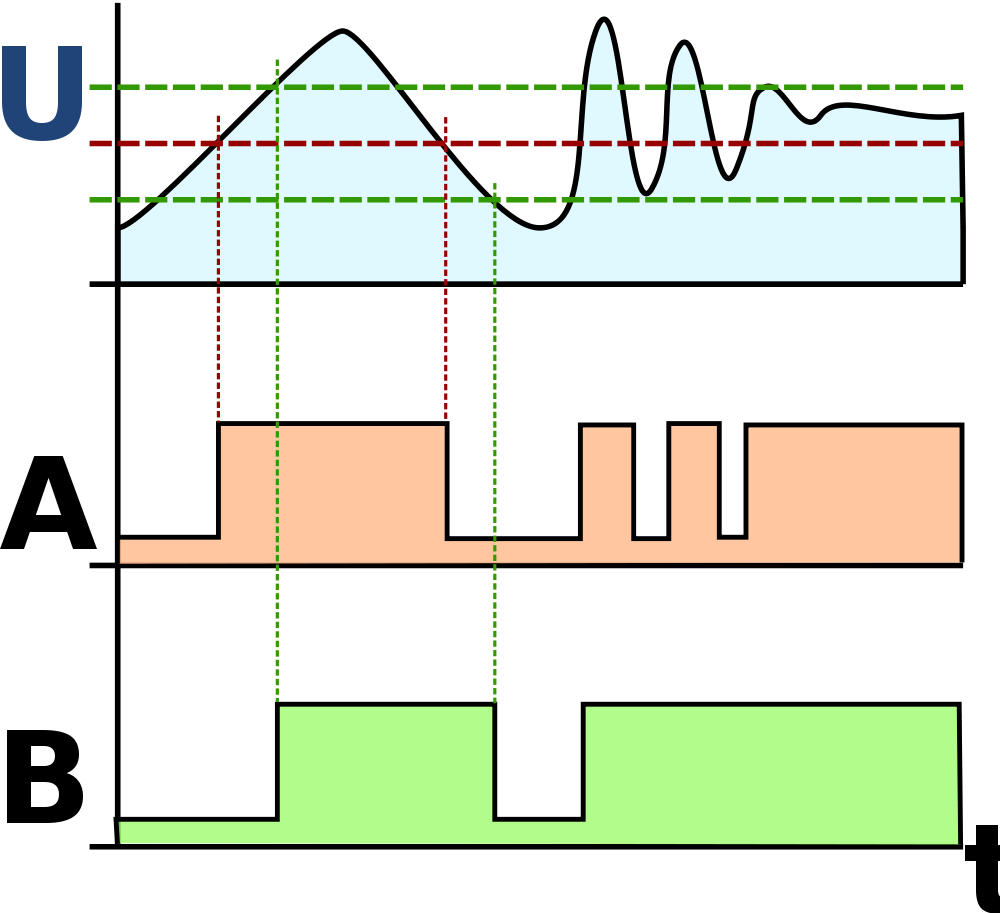
\includegraphics[height=7.5cm]{oskillaattori_pics/1000px-Smitt_hysteresis_graph.png}
%LÄHDE http://en.wikipedia.org/wiki/File:Smitt_hysteresis_graph.svg
\end{center}
}

\frame{
\frametitle{555-ajastinpiiri}
\begin{center}
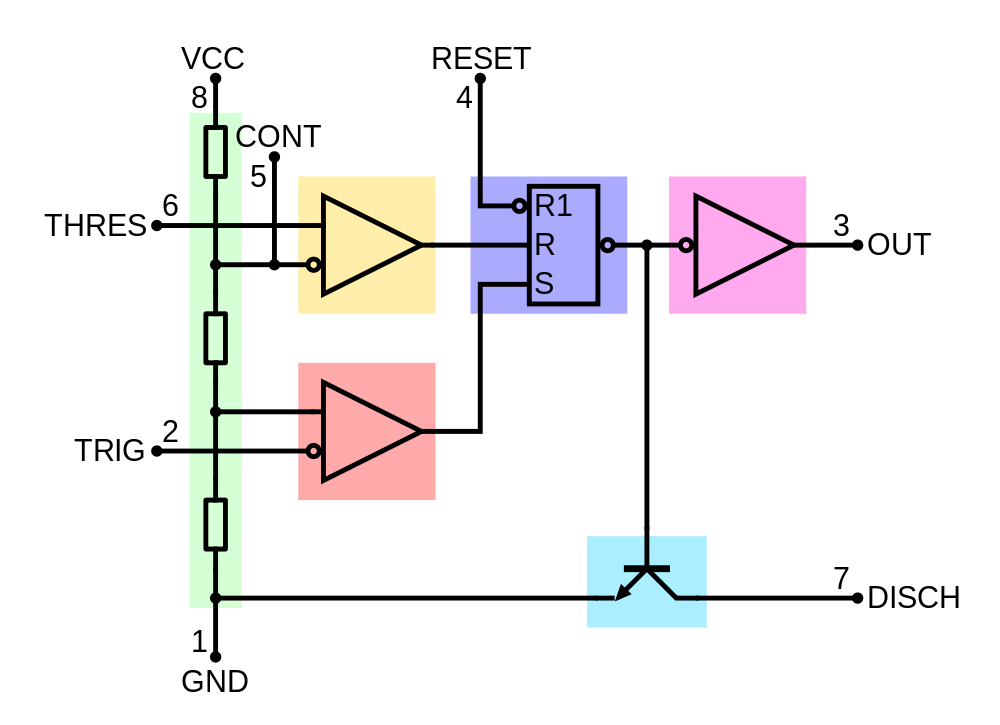
\includegraphics[height=6.5cm]{oskillaattori_pics/1000px-NE555_Bloc_Diagram.png}\\
%LÄHDE: http://en.wikipedia.org/wiki/File:NE555_Bloc_Diagram.svg
\end{center}
}



\frame {
\frametitle{Wienin siltaoskillaattori}

\begin{center}
\begin{picture}(150,200)(50,0)
\ho{50,125}{}
\hz{50,175}{}
\hz{0,175}{\rm PTC}
\hgp{0,175}

\hgp{100,0}
\vz{100,100}{R}
\vc{100,50}{C}

\vc{75,0}{C}
\vz{125,0}{R}
\hln{75,0}{50}
\hln{75,50}{50}

\hln{50,60}{50}
\vln{50,60}{65}

\vln{100,150}{25}
\cn{100,150}
\hln{100,150}{25}
\out{125,150}
\hgp{125,100}
\out{125,100}
\du{125,100}{\Uout}

\dcru{130,0}{U_+=\frac{1}{3+\jj(RC\omega-\frac{1}{RC\omega})}\Uout}

\end{picture}
\end{center}
 }

 \frame{
 \frametitle{Vaihesiirto-oskillaattori}
\begin{center}
\begin{picture}(250,120)(0,0)
\hc{0,50}{C}
\hc{50,50}{C}
\hc{100,50}{C}
\hz{150,50}{R}

\vz{50,0}{R}
\vz{100,0}{R}
\hg{50,0}
\hg{100,0}


\vo{200,30}{}{15}
\hgp{200,30}{}

\hz{200,90}{R_1}

\vln{200,50}{40}
\vln{250,40}{70}

\du{250,-10}{\Uout}
\hg{250,-10}

\hln{0,110}{250}
\vln{0,50}{60}

\end{picture}

\end{center}

 }

\frame{
\frametitle{Yhdenlainen relaksaatio-oskillaattori}

\begin{center}

\begin{picture}(110,130)(50,-50)

\hz{0,20}{R_1\ 1\kohm}
\voi{50,0}{}{15}
\hz{50,60}{R_2\ 15\kohm}
\hgp{50,0}

\hz{100,10}{R_3\ 150 \kohm}
\vo{150,-10}{}{15}
\hgp{150,-10}
\hc{150,50}{C\ 100\ \mbox{nF}}

\vln{200,0}{75}
\hln{100,75}{100}
\vln{150,10}{40}
\vln{0,20}{55}
\hln{0,75}{100}

\vln{50,20}{40}
\vln{100,10}{50}

\hln{200,0}{10}
\du{210,-50}{\Uout}
\hg{210,-50}

\end{picture}
\end{center}

Vasemmalla puolella on Schmitt-liipaisintulolla varustettu komparaattori ja oikealla puolella on integraattori. Yhdessä piirit muodostavat kokonaisuuden, jossa kondensaattori latautuu ja purkautuu jatkuvasti.

}

 \frame{
 \frametitle{Transistorivahvistin (yhteisemitterikytkentä)}
\begin{center}
\begin{picture}(180,160)(-30,-50)

\vz{0,0}{R_2=33\kohm\vspace{-1cm}}
\vz{0,50}{R_1=82\kohm}

\vst{200,0}{12\V}
\vln{200,50}{75}
\vz{100,75}{R_{\rm C}=1\kohm}
\hln{100,125}{100}

\hln{0,125}{100}
\vln{0,100}{25}
\hln{0,50}{50}
\npn{50,50}{}
\hln{0,-50}{200}
\vln{0,-50}{50}
\vln{200,-50}{50}
\vln{100,0}{25}
\vz{100,-50}{R_{\rm E}=470\ohm}

\hc{-50,50}{C_{\rm IN}}
\hc{100,75}{C_{\rm OUT}}
\cn{0,50}

\hln{-100,50}{50}
\du{-100,00}{\Uin}
\hg{-100,0}

\du{150,25}{\Uout}
\hg{150,25}
\hgp{0,-50}

\end{picture}
\end{center}
 }


 \frame{
 \frametitle{Transistorivahvistin}
 \begin{itemize}
 \item Edellisen kalvon piiri vahvistaa vaihtojännitesignaalia $\Uin$.
\item Miksi signaalia ei voi vain syöttää suoraan transistorin kannalle?
\item Mihin piirissä tarvitaan kondensaattoreita?
\item Kuinka suuri on piirin jännitevahvistus $\frac{\Uout}{\Uin}$?
 \end{itemize}
 }

 \frame{
 \frametitle{Transistorivahvistin}
 \begin{itemize}
\item Jotta transistorivahvistin vahvistaisi myös heikkoja signaaleja, se pitää {\em biasoida} eli {\em esijännittää}. Myös termiä {\em tasajänniteasettelu} käytetään.
\item Kondensaattorit estävät esijännitykseen käytettävää tasasähköä vuotamasta vahvistimen tuloon ja lähtöön.
\item Kuvan vahvistinkytkentää kutsutaan yhteisemitteri- eli CE-vahvistimeksi (engl. common emitter).
\item Analysoidaan piirin toimintaa kerrostamismenetelmällä. Mallinnetaan transistoria virtaohjatulla virtalähteellä.
\item Kaikki muut jännitelähteet (kanta-emitteridiodin jännite ja piirin käyttöjännite) asetetaan nollaksi.
\item Oletetaan kondensaattorit oikosuluksi (= signaalin taajuus on niin suuri, että kondensaattorien impedanssi on pieni).
 \end{itemize}
 }


 \frame{
 \frametitle{Transistorivahvistimen analysointi}
\begin{center}
\begin{picture}(180,160)(-30,-50)

\vz{0,0}{R_2=33\kohm\vspace{-1cm}}
\vz{0,50}{R_1=82\kohm}

\vln{200,0}{50}
\vln{200,50}{75}
\vz{100,75}{R_{\rm C}=1\kohm}
\hln{100,125}{100}

\hln{0,125}{100}
\vln{0,100}{25}
\hln{0,50}{50}
\vdj{100,25}{\beta I_{\rm B}}
\hln{50,25}{50}
\vln{50,25}{25}
\ri{75,25}{I_{\rm B}}

\hln{0,-50}{200}
\vln{0,-50}{50}
\vln{200,-50}{50}
\vln{100,0}{25}
\vz{100,-50}{R_{\rm E}=470\ohm}
\hln{-50,50}{50}
\hln{100,75}{50}

\ri{-25,50}{I_{\rm in}}

\cn{0,50}

\hln{-100,50}{50}
\du{-100,00}{\Uin}
\hg{-100,0}

\du{150,25}{\Uout}
\hg{150,25}
\hgp{0,-50}

\end{picture}
\end{center}
 }


 \frame{
 \frametitle{Vahvistuskerroin}
Emitterivirralle voidaan kirjoittaa
\[
\frac{\Uin}{R_{\rm E}}=I_{\rm B}+\beta I_{\rm B} \quad \Rightarrow \quad I_{\rm B}=\frac{\Uin}{R_{\rm E}(1+\beta)}
\]
josta
\[
\Uout = -\beta I_{\rm B}\cdot R_{\rm C}= -\beta \frac{\Uin}{R_{\rm E}(1+\beta)} R_{\rm C}=-\Uin \frac{\beta}{1+\beta} \frac{R_{\rm C}}{R_{\rm E}}
\]
ja
\[
\frac{\Uout}{\Uin}=-\frac{\beta}{1+\beta} \frac{R_{\rm C}}{R_{\rm E}}\approx -\frac{R_{\rm C}}{R_{\rm E}},
\]
koska $\frac{\beta}{1+\beta}\approx 1$.
 }

 \frame{
 \frametitle{Tuloresistanssi}
\[
R_{\rm in}=\frac{\Uin}{I_{\rm in}}
\]
\[
I_{\rm in}=\frac{\Uin}{R_1}+\frac{\Uin}{R_2}+I_{\rm B}=\frac{\Uin}{R_1}+\frac{\Uin}{R_2} +\frac{\Uin}{R_{\rm E}(1+\beta)}
\]
\[
R_{\rm in}=\frac{\Uin}{I_{\rm in}}=\frac{\Uin}{\frac{\Uin}{R_1}+\frac{\Uin}{R_2} +\frac{\Uin}{R_{\rm E}(1+\beta)}}=\frac{1}{\frac{1}{R_1}+\frac{1}{R_2} +\frac{1}{R_{\rm E}(1+\beta)}}
\]

Eli tuloresistanssi on resistanssien $R_1$, $R_2$ ja $R_{\rm E}(1+\beta)$ rinnankytkentä. Voidaan ajatella, että emitterillä oleva resistanssi näkyy kannalla $(1+\beta)$-kertaisena.

 }

 \frame{
 \frametitle{Lähtöresistanssi}
Lähtöresistanssi on helppo johtaa tekemällä kollektorivastukselle ja virtalähteelle lähdemuunnos:
\begin{center}
\begin{picture}(180,160)(100,0)

\vz{100,75}{R_{\rm C}}

\vdj{100,25}{\beta I_{\rm B}}
\hgp{50,125}

\hln{50,125}{50}

\uu{115,75}{\Uout\hspace{-1cm}}
\hgp{100,25}


\vdst{225,50}{\beta I_{\rm B}R_{\rm C}}
\hg{225,50}
\hz{225,100}{R_{\rm C}}
\hg{275,50}
\du{275,50}{\Uout}

\end{picture}
\end{center}
Lähdemuunnoksessa resistanssin arvo säilyy samana, eli vahvistimen lähtöresistanssi on suoraan kollektorivastus $R_{\rm C}$.

 }


 \frame{
 \frametitle{Esimerkki}
\begin{center}
\begin{picture}(180,160)(-30,-50)

\vz{0,0}{R_2=33\kohm\vspace{-1cm}}
\vz{0,50}{R_1=82\kohm}

\vst{200,0}{12\V}
\vln{200,50}{75}
\vz{100,75}{R_{\rm C}=1\kohm}
\hln{100,125}{100}

\hln{0,125}{100}
\vln{0,100}{25}
\hln{0,50}{50}
\npn{50,50}{}
\hln{0,-50}{200}
\vln{0,-50}{50}
\vln{200,-50}{50}
\vln{100,0}{25}
\vz{100,-50}{R_{\rm E}=500\ohm}
\txt{70,25}{\beta=100}

\hc{-50,50}{C_{\rm IN}}
\hc{100,75}{C_{\rm OUT}}
\cn{0,50}

\hln{-100,50}{50}
\du{-100,00}{\Uin}
\hg{-100,0}

\du{150,25}{\Uout}
\hg{150,25}
\hgp{0,-50}

\end{picture}
\end{center}
Kuinka suureksi $C_{\rm IN}$ tulee vähintään valita, jotta yli 20 $\Hz$ taajuiset signaalit eivät vaimene enempää kuin 3 desibeliä piirin ideaalivahvistukseen ($\approx 2$) verrattuna?
 }

\frame{
 \frametitle{Esimerkki}
$C_{\rm IN}$ ja vahvistimen tuloresistanssi $R_{\rm IN}$ muodostavat yhdessä ensimmäisen asteen ylipäästösuodattimen, joka määrää vahvistimen alarajataajuuden. Ensimmäisen asteen suodattimilla suodattimen ominaistaajuus on sama kuin -3 desibelin piste, eli ongelma ratkeaa suoraan laskemalla $C_{\rm IN}$ muodostuneen ylipäästösuodattimen ominaistaajuuden kaavasta ($f_0=20\Hz$):
\[
f_0=\frac{\omega_0}{2\pi}=\frac{\frac{1}{RC}}{2\pi}=\frac{1}{2\pi R C}=\frac{1}{2\pi R_{\rm IN} C_{\rm IN}}\Rightarrow  C_{\rm IN}=\frac{1}{2\pi R_{\rm IN} f_0}
\]
\[
C_{\rm IN}=\frac{1}{2\pi \frac{1}{\frac{1}{R_1}+\frac{1}{R_2} +\frac{1}{R_{\rm E}(1+\beta)}} f_0}\approx 500 \nF
\]

Huomaa, että myös $C_{\rm OUT}$ vaikuttaa alarajataajuuteen, mutta tätä ei käsitelty esimerkissä.


}



% TODO: Yhteisemitterikytkennän piensignaalianalyysin aukilaskenta puuttuu
% TODO: Diodipiirin tarkan ratkaisemisen aukilaskenta puuttuu

\frame{
\frametitle{Diodipiirin ratkaisu "tarkasti"}
\begin{center}
\begin{picture}(180,100)(0,0)

\vst{0,0}{E=1\V}
\hz{25,50}{R=100\ohm}
\hln{75,50}{25}
\hln{0,50}{25}
\dd{100,0}{}
\hln{0,0}{100}
\du{120,0}{U}

\end{picture}
\end{center}

\[
I=I_{\rm S}\left(e^\frac{U}{nU_T}-1\right)\qquad U_T=\frac{{\rm k}T}{\rm q}
\]

\[
I=\frac{E-U}{R}
\]

 }


 \frame{
 \frametitle{Piensignaalianalyysi}
 \begin{itemize}
 \item Kun epälineaarisia komponentteja sisältävän piirin toimintaa tutkitaan, voidaan käyttää joko tarkkoja yhtälöitä (haastavaa, vaatii käytännössä tietokoneen avuksi) tai karkeaa mallia (kuten diodin jännitteen olettaminen 0,7 voltiksi ja transistorin kaava $I_{\rm C}=\beta I_{\rm B}$).
\item Näiden ääripäiden välimuoto on {\em piensignaalianalyysin} käyttäminen.
\item Piensignaalianalyysissä lasketaan ensin komponentin tasajännitetoimintapiste.
\item Tämän jälkeen komponentin ominaiskäyrää (virran riippuvuutta jännitteestä) mallinnetaan ominaiskäyrän derivaatalla.
\item Piensignaalianalyysi antaa kohtuullisen tarkan tuloksen, mikäli signaalitaso on niin pieni\footnote{Tästä nimi piensignaalianalyysi!}, että se ei muuta komponentin toimintapistettä. Toisin sanoen, jos signaalitaso on niin suuri, että ominaiskäyrän derivaatta ja ominaiskäyrä poikkeavat toisistaan paljon, tulos on epätarkka.
 \end{itemize}
 }

\frame{
\frametitle{Diodin piensignaalisijaiskytkentä}

\begin{center}
\begin{picture}(100,40)(0,-10)
\rd{0,0}{}
\ri{10,0}{I}
\rcuu{0,10}{U}
\end{picture}
\end{center}
\[
I=I_{\rm S}\left(e^\frac{U}{nU_T}-1\right)\qquad U_T=\frac{{\rm k}T}{\rm q}
\]
\[
\rm q=1,602\cdot 10^{-19}\, {\rm As}\qquad {\rm k}=1,381
\cdot 10^{-23}\frac{J}{K}
\]
Derivoidaan:
\[
\frac{{\rm d}I}{{\rm d}U} = I_{\rm S}\frac{1}{nU_T}e^\frac{U}{nU_T}=\frac{1}{nU_T}\underbrace{I_{\rm S}e^\frac{U}{nU_T}}_{\approx I}\approx \frac{I}{nU_T}
\]
Koska virta derivoitiin jännitteen suhteen, äsken laskettu suure on konduktanssia. Diodin piensignaaliresistanssi on siis tämän konduktanssin käänteisluku:
\[
r_{\rm d}=\frac{\Delta u}{\Delta i}=\frac{1}{\frac{I}{nU_T}}=\frac{nU_T}{I}
\]

}

 \frame{
 \frametitle{Piensignaalianalyysi diodipiirille}
 \begin{itemize}
 \item Laske ensin diodin tasajännitetoimintapiste: sammuta vaihtojännitelähteet ja laske diodin virta (esimerkiksi) olettamalla johtavan diodin jännitteeksi 0,7 volttia (= tekniikka, joka opeteltiin ensimmäisellä tunnilla).
\item Kun diodin läpi kulkeva (tasa)virta on laskettu, lasketaan diodin dynaaminen resistanssi kaavasta
\[
r_{\rm d}=\frac{nU_T}{I}.
\]
Terminen jännite $U_T$ on huoneenlämmössä noin 26 millivolttia ja emissiovakioksi voi olettaa $n\approx 2$.
\item Lopuksi sammutetaan kaikki tasajännitelähteet, korvataan diodi dynaamisella resistanssilla ja lasketaan vaihtojännitteen vaikutus piiriin.
 \end{itemize}
 }

 \frame{
 \frametitle{Piensignaalianalyysi: yksinkertainen esimerkki}

\begin{center}
\begin{picture}(100,100)(0,0)
\vst{0,0}{E=1 \V}
\vst{0,50}{e_{\rm ac}=100\mV}
\hz{0,100}{R=100\ohm}
\dd{50,0}{}
\hln{0,0}{50}
\vln{50,50}{50}
\dcru{55,0}{U+u_{\rm ac}}
\end{picture}
\end{center}

 }

 \frame{
 \frametitle{Vaihe 1/3}
Sammutetaan vaihtojännitelähde (tai lähteet, jos niitä on useita), ja lasketaan diodin läpi kulkeva tasavirta.

\begin{center}
\begin{picture}(100,100)(0,0)
\vst{0,0}{E=1 \V}
\vln{0,50}{50}
\hz{0,100}{R=100\ohm}
\dd{50,0}{}
\hln{0,0}{50}
\vln{50,50}{50}
\dcru{55,0}{U=0,7 \V}
\di{50,75}{I}
\end{picture}
\end{center}
\[
I=\frac{E-U}{R}=\frac{1 \V - 0,7 \V }{100\ohm}=3\mA
\]

 }

 \frame{
 \frametitle{Vaihe 2/3}
Lasketaan diodin dynaaminen resistanssi:
\[
r_{\rm d}=\frac{nU_T}{I}=\frac{2\cdot 26\mV}{3\mA}\approx 17\ohm
\]

}

 \frame{
 \frametitle{Vaihe 3/3}
 Sammutetaan tasajännitelähde, korvataan diodi dynaamisella resistanssilla ja lasketaan vaihtojännitteen vaikutus piiriin (tässä tapauksessa näppärästi jännitteenjakosäännöllä).
\begin{center}
\begin{picture}(100,100)(0,0)
\vst{0,50}{e_{\rm ac}=100\mV}
\vln{0,0}{50}
\hz{0,100}{R=100\ohm}
\vz{50,0}{r_{\rm d}=17\ohm\hspace{-2.2mm}}
\hln{0,0}{50}
\vln{50,50}{50}
\dcru{55,0}{u_{\rm ac}}
\end{picture}
\end{center}
\[
u_{\rm ac}=e_{\rm ac}\frac{r_{\rm d}}{R+r_{\rm d}}=100\mV\frac{17\ohm}{100\ohm+17\ohm}\approx 15\mV
\]

 }

 \frame{
 \frametitle{Piensignaalianalyysin käytössä huomioitavaa}
Piensignaalianalyysi antaa melko tarkan tuloksen silloin, kun käsiteltävä (vaihtojännite)signaali on amplitudiltaan niin pieni, että se ei muuta piirin toimintapistettä. Toisin sanoen, jos signaalin vaikutusalueella komponentin ominaiskäyrä ja derivaatta poikkeavat toisistaan merkittävästi, piensignaalianalyysi antaa epätarkan tuloksen.

\begin{block}{Esimerkki}
Jos edellisessä esimerkissä vaihtojännitteen amplitudi olisi ollut 10 volttia, piensignaalianalyysin tulos olisi pahasti metsässä. Esimerkiksi voltin amplitudinen sinimuotoinen vaihtojännite pakottaisi diodin estotilaan, jolloin sen dynaaminen resistanssi on satoja kilo-ohmeja tai enemmän.
\end{block}
Piensignaalianalyysi toimii nimensä mukaisesti vain pienillä signaaleilla!
 }
 
 \frame{
 \frametitle{Esimerkki}

\begin{center}
\begin{picture}(100,40)(0,0)
\vst{0,0}{E=10 \V}
\vst{0,50}{e_{\rm ac}=100\mV}
\hz{0,100}{R=1\kohm}
\dd{50,0}{}
\hln{0,0}{50}
\vln{50,50}{50}
\dcru{55,0}{U+u_{\rm ac}}
\end{picture}
\end{center}

Ratkaise piensignaalianalyysin avulla, kuinka suuri on diodin yli vaikuttava vaihtojännite $u_{\rm ac}$.

% (0.052/(9.3/1000))/(1000+(0.052/(9.3/1000)))*0.1
}


 \frame{
 \frametitle{Esimerkki}



Ratkaiseminen tapahtuu kuten edellisen luennon esimerkissä. Lasketaan ensin tasavirta diodin läpi:
\[
I=\frac{10\V-0,7\V}{1\kohm}=9,3\mA
\]
Tasavirran perusteella lasketaan diodin dynaaminen resistanssi:
\[
r_{\rm d}=\frac{nU_T}{I}=\frac{2\cdot 26\mV}{9,3\mA}\approx 5,59 \ohm
\]
Ja ratkaistaan diodin yli oleva vaihtojännite jännitteenjakosäännöllä:
\[
u_{\rm ac}=100\mV\frac{5,59 \ohm}{1\kohm + 5,59 \ohm}\approx 0,556\mV
\]
% (0.052/(9.3/1000))/(1000+(0.052/(9.3/1000)))*0.1
}

 \frame{
 \frametitle{Transistorivahvistimen piensignaalianalyysi}
 \begin{itemize}
  \item Yksinkertaisella sijaiskytkennällä (= pelkkä virtaohjattu virtalähde) CE-transistorivahvistimen analyysi ei anna tarkkaa tulosta, varsinkin jos emitterivastus $R_{\rm E}$ ohitetaan kondensaattorilla tai jätetään pois (vahvistuskerroin olisi mallin mukaan ääretön (muka)).
  \item Ohituskondensaattorin käyttö on erittäin tavallista.
  \item Tarkemman tuloksen saa, kun otetaan huomioon transistorin kanta-emitteridiodin dynaaminen resistanssi.
  \item Transistorilla emissiovakioksi oletetaan yleensä $n\approx 1$.
 \end{itemize}
 }


 \frame{
\frametitle{Epätarkka malli}
\begin{center}
\begin{picture}(100,120)(0,0)
\vdj{50,50}{i_{\rm c}=\beta i_{\rm b}}
\hln{0,50}{50}
\vln{50,0}{50}
\ri{25,50}{i_{\rm b}}
\di{50,25}{i_{\rm b}+i_{\rm c}}

\out{50,0}
\out{50,100}
\out{0,50}
\end{picture}
\end{center}

}

 \frame{
 \frametitle{Tarkempi piensignaalimalli: otetaan huomioon kanta-emitteridiodin dynaaminen resistanssi}
\begin{center}
\begin{picture}(100,120)(0,0)
\vdj{50,50}{i_{\rm c}=\beta i_{\rm b}}
\hln{0,50}{50}
\ri{25,50}{i_{\rm b}}
\vz{50,0}{r_{\rm e}=\frac{nU_T}{I_{\rm E}}}

\out{50,0}
\out{50,100}
\out{0,50}
\end{picture}
\end{center}

Tätä mallia kutsutaan T-sijaiskytkennäksi. On olemassa myös $\pi$-sijaiskytkentä.
}

 \frame{
 \frametitle{Merkinnöistä}
Sopimus:
 \begin{itemize}
 \item Piensignaalianalyysissä tasavirtoja ja -jännitteitä (joista lasketaan piensignaalisijaiskytkennän parametrit, kuten $r_{\rm e}$) merkitään isolla kirjaimella.
\item Piensignaalivirtoja ja -jännitteitä merkitään pienillä kirjaimilla.
\item Esimerkiksi $I_{\rm E}$ on tasavirta, jota käytetään laskettaessa transistorin toimintapistettä.
\item $i_{\rm e}$ on sen sijaan piensignaalivirta (vaihtovirta).
 \end{itemize}
 }



 \frame{
 \frametitle{Transistorivahvistin (yhteisemitterikytkentä)}
\begin{center}
\begin{picture}(180,160)(-30,-50)

\vz{0,0}{R_2=33\kohm\vspace{-1cm}}
\vz{0,50}{R_1=82\kohm}

\vst{200,0}{12\V}
\vln{200,50}{75}
\vz{100,75}{R_{\rm C}=1\kohm}
\hln{100,125}{100}

\hln{0,125}{100}
\vln{0,100}{25}
\hln{0,50}{50}
\npn{50,50}{}
\hln{0,-50}{200}
\vln{0,-50}{50}
\vln{200,-50}{50}
\vln{100,0}{25}
\vz{100,-50}{R_{\rm E}=470\ohm}

\hc{-50,50}{C_{\rm IN}}
\hc{100,75}{C_{\rm OUT}}
\cn{0,50}

\hln{-100,50}{50}
\du{-100,00}{\Uin}
\hg{-100,0}

\du{150,25}{\Uout}
\hg{150,25}
\hgp{0,-50}

\end{picture}
\end{center}
 }

\frame{
 \frametitle{CE-vahvistimen analysointi}
\begin{center}
\begin{picture}(180,160)(-30,-50)

\vz{0,0}{R_2=33\kohm\vspace{-1cm}}
\vz{0,50}{R_1=82\kohm}

\vln{200,0}{50}
\vln{200,50}{75}
\vz{100,75}{R_{\rm C}=1\kohm}
\hln{100,125}{100}

\hln{0,125}{100}
\vln{0,100}{25}
\hln{0,50}{50}
\vdj{100,25}{\beta i_{\rm B}}
\hln{50,25}{50}
\vln{50,25}{25}
\ri{75,25}{i_{\rm B}}

\hln{0,-50}{200}
\vln{0,-50}{50}
\vln{200,-50}{50}
\vln{100,0}{25}
\vz{100,-50}{R_{\rm E}+r_{\rm e}}

\hln{-50,50}{50}
\hln{100,75}{50}

\ri{-25,50}{i_{\rm in}}

\cn{0,50}

\hln{-100,50}{50}
\du{-100,00}{u_{\rm in}}
\hg{-100,0}

\du{150,25}{u_{\rm out}}
\hg{150,25}
\hgp{0,-50}

\end{picture}
\end{center}
 }


\frame{
 \frametitle{Esimerkki: yhteiskollektorikytkentä} % emitterivirta on 3,9 ma ja lopputulos on 15,8 kohm.
\begin{center}
\begin{picture}(180,150)(-30,-50)

\vz{0,0}{R_2=33\kohm\vspace{-1cm}}
\vz{0,50}{R_1=82\kohm}

\vst{200,0}{12\V}
\vln{200,50}{75}
\vz{100,75}{R_{\rm C}=1\kohm}
\hln{100,125}{100}

\hln{0,125}{100}
\vln{0,100}{25}
\hln{0,50}{50}
\npn{50,50}{\beta=100}
\hln{0,-50}{200}
\vln{0,-50}{50}
\vln{200,-50}{50}
\vln{100,0}{25}
\vz{100,-50}{R_{\rm E}=470\ohm}

\hc{-50,50}{C_{\rm IN}}
\hc{100,20}{C_{\rm OUT}}
\cn{0,50}

\hln{-100,50}{50}
\du{-100,00}{\Uin}
\hg{-100,0}

\du{150,-30}{\Uout}
\hg{150,-30}
\hgp{0,-50}


\end{picture}
\end{center}
Laske piensignaalianalyysin avulla kuvan vahvistimelle tulo- ja lähtöresistanssit $R_{\rm in}$ ja $R_{\rm out}$ sekä jännitevahvistus
$\frac{\Uout}{\Uin}$.

%\tiny $R_{\rm in}\approx 15,8\kohm $,  $R_{\rm out}\approx 6,569 \ohm  \approx 7 \ohm$ $\frac{\Uout}{\Uin}\approx 0,99$.
 }
% Wolfram:
% (0.026/((11.3/82000-0.7/33000)/(1/(101*470)+1/33000+1/82000)/470))
% (1/33000+1/82000+1/(101*(6.6621+470)))^-1
% 1/(1/6.6621047841709686024069918877783182438687608855972760509014+1/470.)




\frame{
 \frametitle{Esimerkki}
Lasketaan ensin emitterivirta piensignaalisijaiskytkennän dynaamisen resistanssin $r_{\rm e}$ selvittämiseksi:
\[
I_{\rm E}=(\beta+1)\left( \frac{12\V-U_{\rm E}-0,7\V}{R_1}-\frac{U_{\rm E}+0,7\V}{R_2}  \right)
\]
ja
\[
I_{\rm E}=\frac{U_{\rm E}}{R_{\rm E}}
\]
josta ratkeaa
\[
U_{\rm E}\approx 1,83426\V
\]
ja
\[
I_{\rm E}\approx 3,90 \mA,
\]
joten
\[
r_{\rm e}=\frac{nU_{\rm T}}{I_{\rm E}}\approx\frac{1\cdot 26\mV}{3,9\mA}\approx 6,67 \ohm.
\]
}

\frame{
 \frametitle{Esimerkki} % emitterivirta on 3,9 ma ja lopputulos on 15,8 kohm.
Muodostetaan piensignaalisijaiskytkentä:

\begin{center}
\begin{picture}(180,170)(-30,-50)

\vz{0,0}{R_2=33\kohm\vspace{-1cm}}
\vz{0,50}{R_1=82\kohm}

\vln{200,0}{50}
\vln{200,50}{75}
\vz{100,75}{R_{\rm C}=1\kohm}
\hln{100,125}{100}

\hln{0,125}{100}
\vln{0,100}{25}
\hln{0,50}{50}
\vdj{100,25}{\beta i_{\rm B}}
\hln{50,25}{50}
\vln{50,25}{25}
\ri{75,25}{i_{\rm B}}

\hln{0,-50}{200}
\vln{0,-50}{50}
\vln{200,-50}{50}
\vln{100,0}{25}
\vz{100,-50}{R_{\rm E}+r_{\rm e}}

\hln{-50,50}{50}
\hln{100,25}{50}
\cn{100,25}
\ri{-25,50}{i_{\rm in}}

\cn{0,50}

\hln{-100,50}{50}
\du{-100,00}{u_{\rm in}}
\hg{-100,0}


\du{150,-30}{u_{\rm out}}
\hg{150,-30}
\hgp{0,-50}

\end{picture}
\end{center}

 }

\frame{
 \frametitle{Esimerkki}
Piensignaalikantavirta on
\[
i_{\rm b}=\frac{u_{\rm IN}}{(r_{\rm e}+R_{\rm e})(1+\beta)},
\]
josta saadaan piirin lähtöjännitteksi
\[
u_{\rm out}=i_{\rm e}R_{\rm e}=(1+\beta)i_{\rm b}R_{\rm e}=(1+\beta)\frac{u_{\rm IN}}{(r_{\rm e}+R_{\rm e})(1+\beta)}R_{\rm e}
\]
joten
\[
\frac{u_{\rm out}}{u_{\rm in}}=\frac{R_{\rm E}}{R_{\rm E}+r_{\rm e}}\approx 0,99.
\]
}

\frame{
 \frametitle{Esimerkki}
Lähtöresistanssin selvittämiseksi ajatellaan piirin lähtöön (eli $R_{\rm E}$:n rinnalle) kuormavastus $R_{\rm L}$. Tällöin
kuormalle menevä todellinen lähtöjännite on 
\[
u_{\rm L}=\frac{R_{\rm E}||R_{\rm L}}{R_{\rm E}||R_{\rm L}+r_{\rm e}}u_{\rm in}
\]
Jännitteenjakosäännön mukaan vahvistimen lähtöresistanssille ja kuormittamattomalle jännitteelle pätee
\[
u_{\rm L}=\frac{R_{\rm L}}{R_{\rm OUT}+R_{\rm L}}u_{\rm out}=\frac{R_{\rm L}}{R_{\rm OUT}+R_{\rm L}}\frac{R_{\rm E}}{R_{\rm E}+r_{\rm e}}u_{\rm in}
\]
Edellisistä yhtälöistä ratkeaa
\[
R_{\rm OUT}=\frac{r_{\rm e}R_{E}}{r_{\rm e}+R_{E}}\approx 7\ohm.
\]
}

\frame{
 \frametitle{Esimerkki}
Tuloresistanssi ratkeaa kuten yhteisemitterikytkennässäkin. Nyt myös mahdollinen emitterille kytketty kuorma $R_{\rm L}$ vaikuttaa lähtöresistanssiin:
\[
R_{\rm IN}=R_1||R_2||(1+\beta)(r_{\rm e}+R_{\rm E}||R_{\rm L})
\]
Jos kuormavastusta ei ole kytketty, tuloresistanssiksi saadaan $15,8\kohm$.

}





\frame{
\frametitle{Hakkuritekniikka}
\begin{itemize}
\item Tavallisten verkkomuuntajaan perustuvien teholähteiden ongelmia ovat rajallinen tehontuotto, suuri fyysinen koko sekä paino.
\item Lisäksi suurilla virroilla hurinajännitteen eliminointi vaatisi todella suuren suodatuskondensaattorin.
\item Tasasuuntaamalla verkkojännite sellaisenaan, ja syöttämällä se suurella taajuudella katkottuna muuntajaan, voidaan käyttää fyysisesti pienikokoista suurtaajuusmuuntajaa.
\item Tällaista verkkolaitetta kutsutaan hakkuriteholähteeksi tai hakkuriverkkolaitteeksi.
\item Hakkuritekniikka soveltuu myös tasajännitteen jännitetason laskemiseen sekä -- toisin kuin lineaarinen regulaattoritekniikka -- tasajännitteen jännitetason nostamiseen.
\item Elektroniikan tuotantomenetelmien kehittyminen ja tuotantomäärien kasvaminen on johtanut hintojen laskuun niin, että lähes kaikissa laitteissa on nykyään hakkuriteholähde.

\end{itemize}
}


\frame{
\frametitle{Hakkuriteholähde lyhyesti}
\begin{itemize}
\item Hakkuriteholähteessä jännitteen muuntaminen perustuu nopeaan elektroniseen kytkimeen (transistoriin).
\item Hakkuriteholähteeseen perustuvassa verkkolaitteessa verkkojännite tasasuunnataan, jonka jälkeen se syötetään nopean kytkimen välityksellä suurtaajuusmuuntajaan.
\item Nopean katkomisen ansiosta saadaan muuntajaan suuri magneettivuon muutosnopeus $\to$ pärjätään pienikokoisella muuntajalla.
\item Suuren taajuuden ansiosta myös tarvittavat suodatuskondensaattorit ovat pieniä. Koska jännitteen säätö tapahtuu on-off-kytkimellä, lämpöhäviöt ovat pieniä.
\item Pieni koko ja hyvä hyötysuhde ovat hakkuriteholähteen tärkein etu. Haittapuolia ovat monimutkaisuus ja nopean virran katkomisen tuottamat häiriöt.

\end{itemize}
}

\frame{

\frametitle{Buck- eli step-down-hakkuri}
Jännitettä laskeva hakkuri:

\begin{center}
\begin{picture}(100,100)(0,0)
\pnpb{0,0}{}
\hln{25,50}{25}
\hl{50,50}{}
\ud{50,0}{}
\vc{100,0}{}
\hln{50,0}{50}
\end{picture}
\end{center}

Toteutettavissa esimerkiksi piirillä LM2574.
}

\frame{
\frametitle{Boost- eli step-up-hakkuri}
Jännitettä nostava hakkuri:
\begin{center}
\begin{picture}(100,100)(0,0)
\hl{0,50}{L}
\rd{50,50}{}
\npnnc{5,25}{}
\vc{100,0}{}
\hln{0,0}{100}
\end{picture}
\end{center}

}

\frame{
\frametitle{Buck-boost-hakkuri}
Napaisuuden kääntävä hakkuri:
\begin{center}
\begin{picture}(100,100)(0,0)
\pnpb{0,0}{}
\hln{25,50}{25}
\ld{50,50}{}
\vl{50,0}{}
\vc{100,0}{}
\hln{50,0}{50}
\end{picture}
\end{center}

Toteutettavissa esimerkiksi piirillä LM2574.

}
\frame{
 \frametitle{Vakiovirtalähde}
\begin{center}
\begin{picture}(180,150)(0,-50)

\vz{0,0}{R_{\rm B}=2,2\kohm}
\zud{0,50}{5,1\V}

\vst{200,0}{E=12\V}
\vln{200,50}{75}
\vz{100,75}{R_{\rm E}=2,2\kohm}
\hln{100,125}{100}

\hln{0,125}{100}
\vln{0,100}{25}
\hln{0,50}{50}
\pnpc{50,50}{}
\hln{0,-50}{200}
\vln{0,-50}{50}
\vln{200,-50}{50}
\vln{100,0}{25}
\di{100,0}{I_{\rm L}}
\vz{100,-50}{R_{\rm L}}
\dcru{105,-50}{U_{\rm L}}
\dcru{105,25}{U_{\rm EC}}
\end{picture}
\end{center}

$I_{L}$ pysyy vakiona $R_{\rm L}$:stä riippumatta, kunhan transistori ei mene saturaatioon.

 }


\begin{frame}

Lähtökohtaisesti sähkötyöt ovat kiellettyjä maallikoilta. Lista erikseen sallituista sähkötöistä löytyy esimerkiksi Sähköturvallisuuden edistämiskeskuksen sivuilta
\url{http://www.stek.fi/sahkon_kaytto_kotona/aiotko_tehda_sahkotoita_kotona/fi_FI/sallitut_sahkotyot/}\footnote{Viitattu 14.9.2013}

Listaa ei tarvitse päntätä ulkoa, mutta kokonaiskuva sallituista töistä on hyvä olla mielessä.
\end{frame}


\begin{frame}
\frametitle{Sallitut korjaus- ja asennustyöt}
\begin{itemize}
\item    Yksivaiheisen jatkojohdon korjaus ja teko
\item    Sähkölaitteen rikkoontuneen yksivaiheisen liitäntäjohdon ja pistotulpan vaihto
\item    Valaisimen liitäntäjohdon rikkoontuneen välikytkimen vaihto
\item    Sisustusvalaisimen liittäminen valaisinliitimellä eli ”sokeripalalla”
\item    Kiinteässä asennuksessa valaisinliittimen eli sokeripalan korvaaminen uuden järjestelmän mukaisella valaisinliitinpistorasialla sekä vioittuneen valaisinliitinpistorasian vaihto
\item    Valaisinpistotulpan asennus ja vioittuneen tulpan vaihto
\item    Jännitteettömien pistorasioiden ja kytkimien kansien irrottaminen esim. maalaamisen ja tapetoinnin ajaksi ja rikkoutuneiden kansien vaihto
\item    Suojajännitteisten laitteistojen asentaminen valmistajan tai tavarantoimittajan antamien ohjeiden mukaisesti
\item    Harrastustoimintana tehtävä sähkölaitteiden kokoonpano esim. elektroniikan rakennussarjasta ja tällaisen laitteen korjaaminen
\end{itemize}
\end{frame}



\begin{frame}
\frametitle{Sallitut käyttötoimenpiteet}
\begin{itemize}
\item    Sulakkeen vaihto (tavallisen tulppasulakkeen vaihto tai valonsäätimen sulakkeen vaihto)
\item    Automaattisulakkeen ohjaaminen toiminta-asentoon tai pois päältä
\item    Suojalaitteen toiminta-asennon ohjaaminen
\item    Valaisimen lampun ja sytyttimen vaihto
\item    Jännitteettömyyden toteaminen hyväksytyllä jännitteenkoettimella (koetuskynällä) , kun tehdään jokaiselle sähkönkäyttäjälle sallittuja töitä
\item Vikavirtasuojakytkimen toiminnan testaus
\end{itemize}
\end{frame}

\begin{frame}
\frametitle{Sallittua on myös}
\begin{itemize}
\item    Omakotitalon antennin asentaminen
\item    Sähkölaitteiden mekaanisten osien korjaaminen, esim pesukoneen letkun vaihto, edellyttäen että laitteen kosketussuojaus, vesisuojaus mukaan lukien, ei muutu
\item    Luotettavasti ja kokonaan jännitteettömiksi tehtyjen sähköasennusten purku
\item    Kaapeliojan kaivu ja kaapelin veto maahan. Ennen kaapeliojan peittämistä on sähköalan ammattilaisen todettava, että työ on tehty asianmukaisesti.
\end{itemize}
\end{frame}

\begin{frame}
\frametitle{Laitteiden korjaaminen maallikkona}
Sallittua on
\begin{itemize}
\item Piirikortin vaihto ja lisäys % Ks. Sähkölaitekorjaajan opas s. 5
\item Erilliskoteloidun virtalähteen vaihtaminen.
\item Hybridi- ja sähköajoneuvoissa sellainen huolto- ja korjaustyö, joka on vain pistoliitinkojeen vaihtoa samanlaiseen uuteen, ei vaadi urakointioikeutta (eikä sähkötöiden johtajaa eikä sähköpätevyyttä). Sähköturvallisuudesta on toki huolehdittava ja työntekijöille on annettava SFS 6002:n mukainen sähkötyöturvallisuuskoulutus. % Ks.
\end{itemize}
\end{frame}

\begin{frame}
\frametitle{Sähkölaitteiden suojaustavat}
\begin{itemize}
\item Peruseristys (esim. halpa pöytälamppu).
\item Suojaeristys (parranajokone, porakone)
\item Suojamaadoitus (lämpöpatteri, silitysrauta, sähköhella)
\item Suojajännite (lelut, jouluvalot)
\end{itemize}
\end{frame}

\begin{frame}
\frametitle{Pistotulpat ja kaapelit} % Sähkölaitekorjaajan opas
\begin{itemize}
\item Tavallinen pistotulppa (suojausluokka 0). Ei sovi suojamaadoitettuun pistorasiaan.
\item Suojakosketinpistotulppa (suojausluokka 1).
\item Suojaeristetty pistotulppa (suojausluokka 2).
\end{itemize}

Tavallisen pistotulpan tilalle ei saa vaihtaa suojakosketin- eikä suojaeristettyä pistotulppaa.

Suojaeristetyn pistotulpan tilalle saa vaihtaa suojakosketinpistotulpan. Tällöin suojamaadoitusliitin jätetään kytkemättä.

Verkkojohdon tilalle saa vaihtaa ainoastaan samanlaisen verkkojohdon (mm. johdinpinta-ala, pakkasen-, auringonvalon-, lämmön- ja öljynkestävyys). 

Suojajohdin on jätettävä pidemmäksi kuin muut johtimet, jotta se irtoaa viimeisenä, jos johto revitään väkivalloin irti.

\end{frame}

\begin{frame}
\frametitle{Suojamaadoitus}
\begin{itemize}
\item Käytännössä kaikki metallirunkoiset laitteet ovat suojamaadoitettuja.
\item Jos laitteen sisälle tulee vika, joka meinaa tehdä rungon jännitteiseksi (esimerkiksi leivänpaahtimen vastuslanka katkeaa ja koskee runkoon), vikavirta kulkee rungosta suojamaadoitusliittimen kautta
sähköverkon maahan ja johdonsuojalaite (sulake tai automaattisulake) katkaisee virran.
\item Jos suojamaadoitetun laitteen kytkee tavalliseen pistorasiaan, runko ei ole yhteydessä sähköverkon maahan, ja vian sattuessa runko on jännitteinen $\to$ vaara.
\item Parempi suojaus 
\end{itemize}
\end{frame}

\begin{frame}
\frametitle{Vikavirtasuojakytkin}
\begin{itemize}
\item Pakollinen uudiskohteissa (lähes) kaikissa pistorasioissa.
\item Vikavirtasuojakytkin valvoo vaihe- ja nollajohtimen välistä virtaa. Jos virrat eivät ole yhtä suuret, tämä on merkki viasta (esimerksi ihmisen läpi kulkevasta virrasta) ja vikavirtasuojakytkin katkaisee virran.
\item Vikavirtasuojakytkimiä on saatavilla myös erillisenä pistorasiaan kytkettävänä laitteena. Tällaisen käyttö on suositeltavaa, jos esim. työskentelee ulkona sähkötyökalun kanssa.
\item Vikavirtasuojakytkin suojaa monenlaisilta sähkötapaturmilta. Esimerkiksi kylpyammeeseen putoava hiustenkuivaaja laukaisee välittömästi vikavirtasuojakytkimen.
\end{itemize}
\end{frame}

\begin{frame}
\frametitle{Johtimien merkitseminen}
\begin{itemize}
\item Suojajohdin (PE tai PEN): keltavihreä (ei saa käyttää muuhun!)
\item Nollajohdin (N): sininen
\item Vaihejohtimet (L1, L2, L3): ruskea, musta, harmaa (suositus)
\end{itemize}
Eri aikakausina on käytetty erilaisia värejä, älä luota sokeasti! 

\end{frame}

\begin{frame}
\frametitle{Arkipäivän sähköturvallisuus}
\begin{itemize}
\item Älä sörki avojohtoja.
\item Käytä vikavirtasuojalaitetta, kun käytät sähkötyökaluja.
\item Älä irrota pistotulppaa johdosta vetämällä, vedä aina pistotulpasta.
\item Tarkista aina laite silmämääräisesti. Esimerkiksi murtunut verkkojohto tulee vaihtaa heti. 
\item Varmista jännitteettömyys (koetinkynällä) ennen sähkötöiden tekemistä, ja silloinkin kohtele johtimien metalliosia kuin ne olisivat jännitteisiä.
\item Älä tee sähkötöitä yksin.
\end{itemize}
\begin{block}{Sähkö on turvallista}
Sähkön käyttö on yleisesti ottaen turvallista ja sähkökuolemat harvinaisia. Esimerkiksi kaatumisiin ja putoamisiin kuolee satoja ihmisiä vuodessa ja sähkötapaturmiin alle viisi vuodessa. Tämä ei tarkoita sitä, etteikö kannata olla varovainen.
\end{block}
\tiny \url{http://www.thl.fi/fi_FI/web/pistetapaturmille-fi/tilastot/tilastokatsaukset/kaatumisesta-tai-putoamisesta-aiheutuneet-kuolemat}
\end{frame}

\begin{frame}
\frametitle{Sähkövirran vaikutukset ihmiseen} % D2009
\begin{itemize}
\item Tunto (0,5 mA)
\item Kipu
\item Kouristukset (10 mA)
\item Sydänkammiovärinä (30 mA) ja sydänpysähdys
\item Palovammat ja kemialliset reaktiot (> 100 mA)
\end{itemize}
\end{frame}

\begin{frame}
\frametitle{Ihmiskehon impedanssi}
\begin{itemize}
\item Riippuu kosketuspinta-alasta, henkilöstä, jännitteestä ja taajuudesta.
\item Verkkojännitteellä suuruusluokkaa $1--10\kohm$ % D2009 sivu 45
\end{itemize}
\end{frame}

\begin{frame}
\frametitle{Jännitteet} % SFS 6002
\begin{itemize}
\item Alle 50 Vac tai 120 Vdc = pienoisjännite (ELV)
\item Alle 1000 Vac tai 1500 Vdc = pienjännite (LV)
\item Yli edellä mainituista = suurjännite (HV)
\end{itemize}
\end{frame}

\begin{frame}
\frametitle{Sähkötapaturman ensiapu} % D2009
\begin{itemize}
\item Tee nopea tilannearvio
\item Katkaise virta ja irrota loukkaantunut vaarantamatta itseäsi
\item Tarkista autettavan tila
\item Hälytä apua
\item Anna ensiapua
\end{itemize}
\end{frame}

\begin{frame}
\frametitle{Kuolemaan johtaneet sähkötapaturmat}
Kymmenen vuoden liukuva keskiarvo
\begin{center}
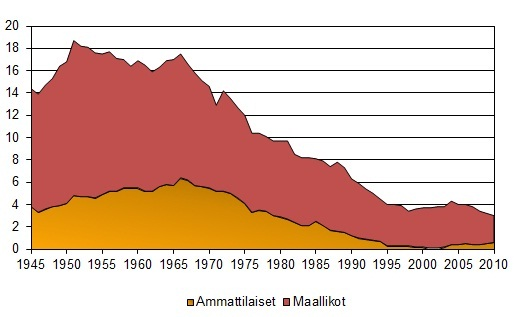
\includegraphics[width=10cm]{sahkoturvallisuus-perusteet_pics/Sahkokuolemat_2010.jpg}
\end{center}

\small \url{http://www.tukes.fi/fi/Rekisterit/sahko-ja-hissit-rekisterit/sahkotapaturmat/kuva-sahkotapaturmat/}
% TODO Mahduta alla olevat kolme riviä siististi kalvolle.
% Kuolemaan johtavien sähkötapaturmien kuvaukset julkistetaan:
% \url{http://www.tukes.fi/fi/Rekisterit/sahko-ja-hissit-rekisterit/sahkotapaturmat/}
% Itsemurhia ei lasketa tapaturmiksi.
\end{frame}

\begin{frame}
\frametitle{Kuolemaan johtaneet sähkötapaturmat 2010}

\begin{itemize}
\item Kytkinlaitosasentaja kuoli latausjännitteeseen valmistellessaan voimajohdon käyttöönottomittausta.
\item Maallikko sai kotipihassaan kuolemaan johtaneen sähköiskun koskettaessaan metallista jatkojohtokelaa. Kela oli tullut jännitteiseksi johtuen siihen tulevan jatkojohdon virheellisestä kytkennästä. 
\item Nuori mies kuoli hypättyään rautatieaseman kävelysillalta alla olevan junan katolle.  
\end{itemize}
\end{frame}

\begin{frame}
\frametitle{Kuolemaan johtaneet sähkötapaturmat 2009}
\begin{itemize}
\item Verkkoyhtiön kolmesta sähköasentajasta koostuva työryhmä oli asentamassa sähköliittymien etäluennan käyttöönottoon liittyvää laitetta 20 kV pylväsmuuntajan kanteen. Työkohde erotettiin muuntajaerottimella (kuormanerotin) ja erottimen avausväli tarkastettiin silmämääräisesti. Muuntajan jännitteettömyyttä ei kuitenkaan varmistettu eikä kohdetta työmaadoitettu ennen töiden aloittamista, minkä seurauksena yksi sähköasentajista sai muuntajaa syöttävästä johdosta tappavan sähköiskun. Johdin oli jännitteinen, koska muuntajan pylväserottimen kolmesta vaiheesta yksi ei ollut auennut.

\item  Nuori mieshenkilö oli jostain syystä kiivennyt aamuyöllä asemalla seisoneen tavarajunan katolle. Hän sai vaunun katolla kuolettavan sähköiskun ja putosi maahan.
\end{itemize}
\end{frame}

\begin{frame}
\frametitle{Kuolemaan johtaneet sähkötapaturmat 2007}
Vuonna 2008 ei sähkökuolemia!
\begin{itemize}
\item Mies menehtyi asunnossaan omatoimisen keittiöremontin yhteydessä. Hän sai sähköasennusten jännitteisestä johdosta sähköiskun, joka meni kädestä käteen. Mies kuoli sairaalassa.
\end{itemize}
\end{frame}


\begin{frame}
\frametitle{Sähköpätevyydet}
Sähkötöiden johtajalla ja käytön johtajalla on oltava riittävä kelpoisuus. Pätevyystodistuksen myöntää Seti Oy. Pätevyyteen vaaditaan
\begin{itemize}
\item Riittävä koulutus
\item Riittävä työkokemus
\item Hyväksytysti suoritettu sähköturvallisuustutkinto
\end{itemize}
\end{frame}

\begin{frame}
\frametitle{Sähköpätevyys 3}
Koulutus ja työkokemus
\begin{itemize}
\item Soveltuva korkeakoulututkinto + 6 kk sähkötyökokemusta.
\item Sähköalan insinööri- tai teknikkotutkinto + 6 kk.
\item Soveltuva (erikois)ammattitutkinto + 6 kk.
\item Soveltuva ammatillinen perustutkinto + 1 v.
\item {\em Riittävät alan perustiedot} + 6 vuotta sähkötyökokemusta.
\end{itemize}
\end{frame}

\begin{frame}
\frametitle{Vaatimukset opinnoille}
Kk-tutkinnossa 45 opintopistettä sähköalan opintoja (harjoittelua ja opinnäytetyötä ei lasketa). Opinnoissa on käsiteltävä mm. seuraavat aiheet
\begin{itemize}
\item Teoreettinen sähkötekniikka ja sähkömittaustekniikka
\item Sähköturvallisuussäädökset ja -standardit
\item Sähkötyöturvallisuus
\item Rakennuksen sähköverkko
\item Sähköturvallisuuteen liittyvät tarkastukset
\end{itemize}
Tarkempi lista vaadittavista opinnoista löytyy Henkilö- ja yritysarviointi Seti:n sivuilta \url{http://seti.fi}. Täydentäviä opintoja voi suorittaa myös valmistumisen jälkeen. Oppilaitos antaa pyydettäessä todistuksen, jossa kerrotaan, että opinnot on täydennetty vaatimuksia vastaavaksi.
\end{frame}



\begin{frame}
\frametitle{Lähteitä ja lisälukemista}
Jos sähköturvallisuus kiinnostaa lisää, kannattaa tutustua seuraaviin kirjoihin:

\begin{itemize}
\item {\bf SFS 6002 käytännössä. Sähköinfo Oy. 10. uusittu painos. 2010.} Lyhyt käytännön sähköturvallisuuteen keskittyvä kirja.
\item {\bf D1-2012 Käsikirja rakennusten sähköasennuksista. Sähköinfo Oy. 19. uusittu painos. 2012.} Paksu mutta helppolukuinen ja käytännönläheinen kirja sähköasennuksista ja sähköturvallisuudesta.
\item {\bf Sähkölaitekorjaajan opas. Sähköinfo Oy. 7. uusittu painos. 2010.} 19-sivuinen käytännönläheinen opas sähkölaitteiden korjaamiseen.
\end{itemize}
\end{frame}


\frame{
\frametitle{Diodi}
\begin{itemize}
\item Puolijohdediodi koostuu p- ja n-tyyppisen puolijohdepalasen rajapinnasta. n-tyyppisessä puolijohteessa on varauksenkuljettajina elektroneja ja p-tyyppisessä
aukkoja.
\item pn-liitoksessa virta voi kulkea vain toiseen suuntaan (pientä vuotovirtaa lukuunottamatta). Jos jännitteen kytkee toisin päin,
liitoksen ympärille muodostuu tyhjennysalue, ja varauksenkuljettajat eivät pääse liikkumaan.
\item Jos $U$ on positiivinen, sitä kutsutaan {\bf päästösuuntaiseksi} jännitteeksi, jos negatiivinen, {\bf estosuuntaiseksi}.
\end{itemize}

\begin{center}
\begin{picture}(100,40)(0,-10)
\rd{0,0}{}
\ri{10,0}{I}
\rcuu{0,10}{U}
\end{picture}
\end{center}
\[
I=I_{\rm S}\left(e^\frac{U}{nU_T}-1\right)\qquad U_T=\frac{{\rm k}T}{\rm q}
\]
\[
\rm q=1,602\cdot 10^{-19}\, {\rm As}\qquad {\rm k}=1,381
\cdot 10^{-23}\frac{J}{K}
\]

}

\frame{
\frametitle{Diodi}
\begin{itemize}
\item Puolijohdediodin yhtälöjen käyttö on hankalaa käsin laskiessa. Epälineaarista yhtälöryhmää
ei voi ratkaista analyyttisesti (=kaavaa pyörittämällä) vaan on käytettävä iteratiivisia menetelmiä.
\item Diodin jännite-virtakäyrä nousee jyrkästi n. 0,7-0,8 voltin kohdalla.
\item Käsinlaskiessa voidaan käyttää paloittain lineaarista sijaiskytkentää,
jossa diodin yli on esimerkiksi 0,7 voltin vakiojännite, jos sen läpi kulkee
virta päästösuuntaan.
\item Tässä materiaalissa käytämme diodille sellaista paloittain lineaarista sijaiskytkentää,
jossa diodin läpi kulkee virta ainoastaan päästösuuntaan ja jos virta
kulkee, diodin yli on 0,7 voltin jännite.

\end{itemize}

}

\frame{
\frametitle{Laskutekniikkaa}
Paloittain lineaarista sijaiskytkentää sovelletaan seuraavasti:
\begin{itemize}
\item Irroita diodi piiristä.
\item Laske jännite, joka muodostuu diodin elektrodien välille (siis siihen kohtaan, josta
diodi otettiin pois).
\item Jos tämä jännite on suurempi tai yhtä suuri kuin 0,7 volttia, diodi johtaa, ja
sen yli muodostuu 0,7 voltin jännite, kun se laitetaan takaisin piiriin.
\item Jos jännite on pienempi kuin 0,7 volttia, diodi ei johda eikä sen läpi kulje virtaa.
\end{itemize}
Jos piirissä on useita diodeja, menettely pitää toistaa jokaiselle diodille erikseen,
niin että tiedetään, mitkä diodeista johtavat.

}

\frame{
\frametitle{Esimerkki}
\begin{center}
\begin{picture}(180,100)(0,0)

\vst{0,0}{E=12\V}

\hz{0,50}{R}
%\txt{75,70}{C\ 1\,\mathrm{nF}}
%\hso{0,50}{K}
\hln{50,50}{50}
\dd{100,0}{}
\put(87,20){\vector(-1,-1){10}}
\put(87,27){\vector(-1,-1){10}}


\hln{0,0}{100}
\du{120,0}{U_{\rm LED}}


\end{picture}
\end{center}

Valmistajan datalehden mukaan kuvan ledin nimellisjännite 10 mA virralla on 2,0 volttia.
Kuinka suuri vastuksen R on oltava, jotta ledin läpi kulkisi 10 mA virta?

{\bf Ratkaisu:} $R=\frac{12\V-2,0\V}{10\mA}=1\kohm$.
}

\frame{
\frametitle{Toinen esimerkki}
\begin{center}
\begin{picture}(150,100)(0,0)

\vz{0,50}{\al{R_1}{5\kohm}}
\vz{0,0}{\al{R_2}{7\kohm}}
%\hz{25,50}{\al{R_5}{1,\!5 \kohm}\vspace{2.5cm}}
\rd{25,50}{}
\vz{100,50}{\al{R_3}{4\kohm}\hspace{-1.7cm}}
\vz{100,0}{\al{R_4}{8\kohm}}
\ri{25,50}{I}
%\di{100,50}{I_3}
\hln{0,50}{25}
\hln{75,50}{25}
\hln{0,0}{150}
\hln{0,100}{150}
\vst{150,25}{\al{E}{12\V}\hspace{-1.7cm}}
\vln{150,0}{25}
\vln{150,75}{25}

%\dcru{5,0}{U_{\mathrm{A0}}}
%\dcru{105,0}{U_{\mathrm{B0}}}

\end{picture}

\end{center}
a) Kuinka suuri on virta $I$?\\
b) Käännetään diodi toisin päin. Kuinka suuri on nyt virta diodin läpi?

\vfill


}


\frame{
\frametitle{Toinen esimerkki}
\begin{center}
\begin{picture}(150,100)(0,0)

\vz{0,50}{\al{R_1}{5\kohm}}
\vz{0,0}{\al{R_2}{7\kohm}}
%\rd{25,50}{}
\out{25,50}
\out{75,50}
\vz{100,50}{\al{R_3}{4\kohm}\hspace{-1.7cm}}
\vz{100,0}{\al{R_4}{8\kohm}}
%\ri{25,50}{I}
\ru{25,50}{E_{\rm T}}
\hln{0,50}{25}
\hln{75,50}{25}
\hln{0,0}{150}
\hln{0,100}{150}
\vst{150,25}{\al{E}{12\V}\hspace{-1.7cm}}
\vln{150,0}{25}
\vln{150,75}{25}

%\dcru{5,0}{U_{\mathrm{A0}}}
%\dcru{105,0}{U_{\mathrm{B0}}}

\end{picture}
\end{center}

Irrotetaan diodi piiristä ja muodostetaan loppupiiristä Théveninin lähde. Lähdejännite saadaan jännitteenjakosäännön avulla. Lasketaan $R_2$:n ja $R_4$:n yli olevat jännitteet, ja niiden erotuksena saadaan Théveninin lähdejännite $E_{\rm T}$:
\[
E_{\rm T}=E\frac{R_2}{R_1+R_2}-E\frac{R_4}{R_3+R_4}=-1\V.
\]
a) Koska jännite on estosuuntainen, diodi ei johda $\to$ $I=0A$.
}

\frame{
\frametitle{Toinen esimerkki}
\begin{center}
\begin{picture}(150,100)(0,0)

\vz{0,50}{\al{R_1}{5\kohm}}
\vz{0,0}{\al{R_2}{7\kohm}}
%\rd{25,50}{}
\out{25,50}
\out{75,50}
\vz{100,50}{\al{R_3}{4\kohm}\hspace{-1.7cm}}
\vz{100,0}{\al{R_4}{8\kohm}}
%\ri{25,50}{I}
%\ru{25,50}{E_{\rm T}}
\hln{0,50}{25}
\hln{75,50}{25}
\hln{0,0}{150}
\hln{0,100}{150}
%\vst{150,25}{\al{E}{12\V}\hspace{-1.7cm}}
\vln{150,0}{75} %25
\vln{150,75}{25}

%\dcru{5,0}{U_{\mathrm{A0}}}
%\dcru{105,0}{U_{\mathrm{B0}}}

\end{picture}
\end{center}

B-kohdassa diodi käännetään toisin päin, jolloin kynnysjännite 0,7 V ylittyy ja diodi johtaa. Virran selvittämiseksi lasketaan Théveninin resistanssi $R_{\rm T}$ sammuttamalla lähde $E$ ja laskemalla diodin kiinnityskohdan resistanssi:
\[
R_{\rm T}=R_1||R_2+R_3||R_4=\frac{1}{\frac{1}{R_1}+\frac{1}{R_2}}+\frac{1}{\frac{1}{R_3}+\frac{1}{R_4}}=\frac{67}{12}\kohm\approx 5,58\kohm
\]
jolloin virta $I=-\frac{1\V-0,7\V}{\frac{67}{12}\kohm}\approx -53,7\,{\mu \rm A}.$
}



\frame{
\frametitle{Erikoisdiodeja}
\begin{description}
\item[Zenerdiodi] johtaa myös estosuuntaan, jos zenerjännite ylittyy.
\item[Varaktori] eli kapasitanssidiodi. Voidaan käyttää jännitteellä
säädettävänä kondensaattorina.
\item [Led] eli hohtodiodi lähettää valoa, kun sen läpi kulkee päästösuuntainen virta.
\item[Fotodiodi] on diodi, jonka estosuuntainen virta riippuu diodiin osuvan valon voimakkuudesta.
\item[Schottky-diodi] on valmistettu metallin ja puolijohteen liitoksesta, ja sille on tyypillistä
matala päästösuuntainen jännite.
\end{description}

}


 \frame{
 \frametitle{Diodisovelluksia}
 \begin{itemize}
 \item Tasasuuntaus (ja demodulaatio)
 \item Ylijännitesuojaus
\item Tarkkuustasasuuntaaja ja näytteenotto- ja pitopiiri
\item Lämpötila-anturina toimiminen
\item Jännitereferenssinä toimiminen
 \end{itemize}
 }

 \frame{
 \frametitle{Puoliaaltotasasuuntaus}
\begin{center}
%\begin{picture}(180,100)(0,0)
%\vmlc{0,0}{}
%\rd{40,50}{}
%\hln{40,0}{50}
%\vz{90,0}{}
%\hln{-50,0}{50}
%\hln{-50,50}{50}
%\end{picture}
% Commonsissa paljon parempi kuva.
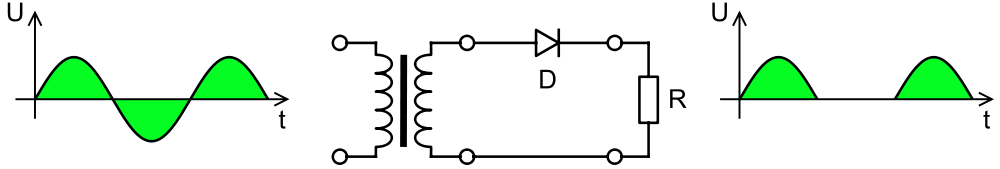
\includegraphics[width=\linewidth]{diodi_pics/1000px-Halfwave-rectifier-en-svg.png}
\end{center}

Käytännössä diodin kynnysjännite vaikuttaa tasasuunnattuun jännitteeseen. Kun muuntajalta saatavan jännitteen arvo laskee alle diodin kynnysjännitteen, tasasuuntaajan ulostulojännite on nolla volttia.

\let\thefootnote\relax\footnotetext{\tiny Kuva: \url{http://commons.wikimedia.org/wiki/File:Halfwave.rectifier.en.svg}}
 
 }

 \frame{
 \frametitle{Diodin käyttö ilmaisimena, "kidekone"}
\begin{center}
\begin{picture}(180,100)(0,0)


\vc{50,0}{}
\vl{100,0}{}
\rd{100,50}{}
\vc{150,0}{}
\vz{200,0}{}
\hln{50,0}{150}
\hln{50,50}{50}
\hln{150,50}{50}

\hgp{50,0}{}
\hln{0,50}{50}
\vln{0,50}{25}

\end{picture}
\end{center}
 }

 \frame{
 \frametitle{Kokoaaltotasasuuntaus}
\begin{center}
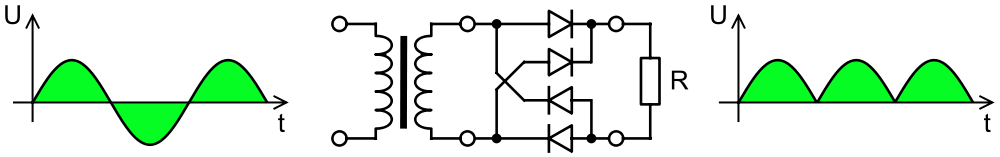
\includegraphics[width=\linewidth]{diodi_pics/1000px-Gratz-rectifier-en-svg.png}
\end{center}
\let\thefootnote\relax\footnotetext{\tiny Kuva: \url{http://commons.wikimedia.org/wiki/File:Gratz.rectifier.en.svg}}
 }

 \frame{
 \frametitle{Kokoaaltotasasuuntaus keskiulosotolla}
\begin{center}
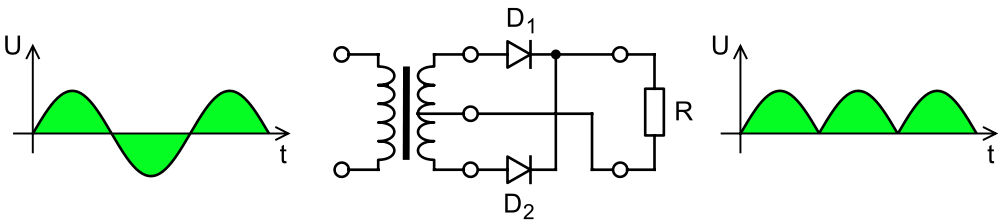
\includegraphics[width=\linewidth]{diodi_pics/1000px-Fullwave-rectifier-en-svg.png}
\end{center}
\let\thefootnote\relax\footnotetext{\tiny Kuva: \url{http://commons.wikimedia.org/wiki/File:Fullwave.rectifier.en.svg}}
 }

 \frame{
 \frametitle{Tarkkuustasasuuntaaja ja näytteenotto- ja pitopiiri}
 \begin{itemize}
 \item Operaatiovahvistimen ja diodi(e)n avulla voidaan toteuttaa myös {\em tarkkuustasasuuntaaja} sekä {\em näytteenotto- ja pitopiiri}.
 \end{itemize}
 }

 \frame{
 \frametitle{Tulon ylijännitesuojaus}
\begin{center}
\begin{picture}(200,100)(0,0)
\hln{0,0}{200}
\hln{0,50}{100}
\hln{50,100}{150}

\out{0,50}{}
\out{0,0}{}


\ud{50,50}{}
\ud{50,0}{}
\cn{50,50}

\vst{200,00}{\mbox{\tiny käyttöjännite}}

\put(100,0){\dashbox(75,75)}

\vln{200,50}{50}

\vln{137,75}{25}

\end{picture}
\end{center}



 }



 \frame{
 \frametitle{Lämpötilan mittaaminen}
 \begin{itemize}
 \item Lämpötila vaikuttaa diodin jännitteeseen, jos virta pidetään vakiona (ja päinvastoin).
 \end{itemize}
 }

 \frame{
 \frametitle{Jännitereferenssi zenerdiodilla}
\begin{center}
\begin{picture}(180,100)(0,0)
\zud{0,0}{}
\vz{0,50}{R}

\dcru{25,0}{U_{\rm Z}}

\vst{-50,25}{U}
\vln{-50,0}{25}
\vln{-50,75}{25}

\hln{-50,0}{50}
\hln{-50,100}{50}


\end{picture}
\end{center}
Jännite $U_{\rm Z}$ pysyy lähes vakiona, vaikka $U$ vaihtelee. Toiminta perustuu zenerdiodin jyrkkään ominaiskäyrään: zenerdiodin jännite ei juuri muutu, vaikka virta muuttuu.
 }


\frame{
\frametitle{Käytännön diodit}
Puolijohdediodin valintaan vaikuttavat muun muassa seuraavat ominaisuudet
\begin{itemize}
\item Virrankesto/tehonkesto
\item Jäähdytettävyys
\item Estosuuntaisen jännitteen kesto
\item Estosuuntainen kapasitanssi
\item Elpymisaika, "nopeus"
\end{itemize}
}

\frame{
\frametitle{Virrankesto, tehonkesto ja jäähdytettävyys}
\begin{itemize}
\item Liian korkea lämpötila tuhoaa komponentin.
\item Tavallinen pikkudiodi kestää suuruusluokkaa 1 W tehon.
\item Tällainen komponentti jäähtyy pääasiassa kytkentälankojen kautta.
\item Suurilla tehoilla tarvitaan jäähdytysripa ja vielä suuremmilla pakotettu ilmajäähdytys.
\item Datalehdessä yleensä arvot jatkuvalle ja hetkelliselle maksimiteholle.
\end{itemize}
}

\frame{
\frametitle{Jännitteenkesto}
\begin{itemize}
\item Liian voimakas sähkökenttä rajapinnassa aikaansaa läpilyönnin $\to$ suuri virta $\to$ komponentti palaa rikki.
\item Hallittua läpilyöntiä käytetään hyväksi zenerdiodeissa.
\end{itemize}
}

\frame{
\frametitle{Estosuuntainen kapasitanssi}
\begin{itemize}
\item Suurtaajuussovelluksissa on merkitystä rajapinnan kapasitanssilla.
\item Ilmiötä käytetään hyväksi kapasitanssidiodissa.
\end{itemize}
}


\frame{ % http://www.tokem.fi/teku/virt_amk/elko/Kurssin_sisalto/Aktiiviset/Diodit/diodit.html
\frametitle{Elpymisaika}
\begin{itemize}
\item Kun päästösuuntaan johtavassa diodissa jännite kytketään yhtäkkiä toisin päin, virta kulkee vielä hetken.
\item Schottky-diodeilla on lyhyt elpymisaika (ja matala päästösuuntainen jännite)
\end{itemize}
}

\frame{
\frametitle{Tutustu kahden  "klassikkodiodin"\ datalehtiin}
\begin{itemize}
\item Piensignaalidiodi 1N4148
\item Tasasuuntausdiodi 1N4007 
\end{itemize}
}

\frame{
\frametitle{Operaatiovahvistimen epäideaalisuudet}
Ideaalinen operaatiovahvistin
\begin{itemize}
\item on äärettömän nopea.
\item $A \to \infty$
\item Tulonapoihin ei mene virtaa
\item  Lähtövirta ja -jännite voi olla kuinka suuri tahansa
\end{itemize}
Negatiivisesti takaisinkytkettynä ideaalisen operaatiovahvistimen tulonavoissa on täsmälleen sama jännite.
}

\frame{
\frametitle{Käytännön operaatiovahvistin}
\begin{itemize}
\item On hidas
\item Vahvistuskerroin $A$ on suuri muttei ääretön.
\item Tulonapoihin menee pieni virta.
\item Lähtövirta on rajallinen, kuten myös lähtöjännite.
\item Tulonavat eivät ole samassa potentiaalissa, vaan niiden välillä on pieni jännite-ero.
\end{itemize}
}

\frame{
\frametitle{Tulonsiirrosjännite}
\begin{itemize}
\item Negatiivisesti takaisinkytketyn operaatiovahvistimen tulonapojen välillä on pieni jännite, jota kutsutaan
offset-jännitteeksi eli tulonsiirrosjännitteeksi.
\item Suuruusluokka on muutamasta millivoltista satoihin mikrovoltteihin.
\item Joissain operaatiovahvistimissa on liitännät potentiometrille, jolla voidaan nollata tulonsiirrosjännite.
\item Joissain malleissa on automaattinen offset-jännitteen nollaus.
\item $U_{\rm offset}=U_+-U_-$.
\end{itemize}
}

\frame{
\frametitle{Tuloesivirta ja tulonsiirrosvirta}
\begin{itemize}
\item Molempiin tulonapoihin menee pieni virta. Virrat eivät ole samansuuruisia ($I_+ \not = I_-$).
\item Tuloesivirta = $\frac{I_+ -  I_-}{2}$
\item Tulonsiirrosvirta = $I_+ -  I_-$
\item Virrat ovat yleensä nanoampeeriluokkaa.
\end{itemize}
}

\frame{
\frametitle{Toteutustavat}
\begin{itemize}
\item Bipolaaritransistorioperaatiovahvistimilla offset-jännite on yleensä pieni ja tulovirrat suurempia kuin kanavatransistorioperaatiovahvistimilla, joilla puolestaan offset-jännite voi olla suurehko.
\end{itemize}
}

\frame{
\frametitle{Äärellinen nopeus}
\begin{itemize}
\item Operaatiovahvistimen lähtöjännite ei voi muuttua äärettömän nopeasti.
\item Slew rate eli seurantanopeus kertoo, kuinka nopeasti operaatiovahvistimen lähtöjännite voi muuttua.
\item Suuruusluokka on voltteja tai kymmeniä voltteja per mikrosekunti.
\end{itemize}
}


\frame{
\frametitle{Äärellinen lähtövirta ja lähtöjännite}
\begin{itemize}
\item Lähtöjännite ei voi mennä ylitse (eikä alitse) käyttöjännitteiden.
\item Kaikilla operaatiovahvistimilla lähtöjännite ei yllä edes käyttöjännitteisiin.
\item Jos lähtöjännite yltää molempiin käyttöjännitteisiin, puhutaan rail-to-rail -operaatiovahvistimesta.
\item Lähtövirta on myös äärellinen.
\end{itemize}
}

\frame{
\frametitle{CMRR}
\begin{itemize}
\item Common Mode Rejection Ratio eli yhteismuodon vaimennussuhde.
\item Ideaalinen operaatiovahvistin vahvistaa vain jännite-eroa, ei yhteismuotoista tulojännitettä.
\item CMRR = $\frac{A_{\rm D}}{A_{\rm C}}$.
\item Ilmoitetaan yleensä desibeleinä, kuten myös käyttöjännitteen vaimennussuhde (PSRR), joka kertoo, kuinka
paljon käyttöjännitteen heilahtelu näkyy lähtöjännitteessä.
\end{itemize}
}

\frame{
\frametitle{Desibeli}
\begin{itemize}
\item Desibeli on dimensioton yksikkö, joka kuvaa tehosuureiden suhdetta logaritmisella asteikolla.
\item Desibeleistä puhuttaessa pitää aina tietää vertailuun käytetty teho.
\item Teho desibeleinä:
\[
10\log_{10} \frac{\rm teho}{\rm vertailuteho}=10\log_{10} \frac{P}{P_{\rm ref}}
\]
\item Radiotekniikassa yleinen yksikkö on dBm, mikä tarkoittaa tehoa verrattuna yhden milliwatin tehoon.
\item Esimerkiksi 1 watin teho on $10\log_{10} \frac{1\, \rm W}{1\, \rm mW}=30\, \rm dBm$
\end{itemize}
}

\frame{
\frametitle{Amplitudisuureet desibeleinä}
\begin{itemize}
\item Teho on verrannollinen amplitudin neliöön (esimerkiksi ääniteho on verrannollinen äänenpaineen neliöön ja vastuksen teho on verrannollinen virran tai jännitteen neliöön).
\item Amplitudeista puhuttaessa desibeliyksikössä on kertoimena 20, ei 10. Esimerkiksi sähköteholle ja virralle:
\[
10\log_{10} \frac{P}{P_{\rm ref}}=10\log_{10} \frac{RI^2}{RI_{\rm ref}^2}=10\log_{10} \Bigg(\frac{I}{I_{\rm ref}}\Bigg)^2=20\log_{10} \frac{I}{I_{\rm ref}}
\]
\item Radiotekniikassa käytetään jännitetasojen ilmaisemiseen mm. desibelimikrovoltteja. Esimerkiksi 1 voltti on
\[
20\log_{10} \frac{1\,\rm V}{1\, \rm \mu V}= 120\, \rm dB\mu V
\]

\end{itemize}
}

\frame{
\frametitle{Komponenttien jäähdytys}
\begin{itemize}
\item Lämmöntuotanto on ongelma monessa elektronisessa laitteessa (audiovahvistimet, tietokoneet, sähkömoottorin ohjauselektroniikka).
\item Nyrkkisääntö: TO-3-kotelo kestää jäähdyttämättömänä noin 3 W ja TO-220-kotelo noin 2 W tehon.
\item Suurtehosovelluksissa käytetään pakotettua ilmajäähdytystä (=tuuletinta) tai nestejäähdytystä.
\item Muutamien kymmenien wattien lämpöteho voidaan käsitellä passiivisella ilmajäähdytyksellä, mikäli laitteen kotelo pääsee tuulettumaan hyvin.
\item Lämmön johtumista pois komponentista ympäristön ilmaan mallinnetaan {\bf lämpöresistanssilla}.
\end{itemize}
}

\frame{
\frametitle{Lämpöresistanssi}
\begin{itemize}
\item Lämmön johtumista pois komponentista voidaan mallintaa melko hyvin lineaarisella mallilla, jossa komponentin ja jäähdytyselementin muodostaman lämmönsiirtopiirin lämmönjohtavuutta (tai oikeastaan sen käänteislukua) mallinnetaan lämpöresistanssilla.
\item Yhden watin tehonlisäys komponentissa kasvattaa komponentin ja ympäristön lämpötilaeroa koko lämmönsiirtopiirin lämpöresistanssin osoittamalla määrällä
\[
\Delta T=\theta \cdot P
\]
\item $\Delta T$=lämmönlähteen (=puolijohteen) ja ympäristön (=ilman) lämpötilaero.
\item $\theta$=Lämmönsiirtopiirin lämpöresistanssi, joka koostuu komponentin kotelon, kotelon ja jäähdytyselementin välisen liitoksen sekä jäähdytyselementin lämpöresistanssista.
\item $P=$ komponentin lämpenemisteho.
\end{itemize}
}

\frame{
\frametitle{Lämpöresistanssi: laskuesimerkki}
TO-3-kotelossa oleva puolijohdekomponentti kuumenee 15 watin teholla. Lämpöresistanssi puolijohteesta TO-3-koteloon on $\theta_{\rm JC}=2\ ^\circ \rm C /W$, komponentin ja jäähdytyslevyn liitoksen lämpöresistanssiksi oletetaan $\theta_{\rm CS}=1\ ^\circ \rm C /W$ ja jäähdytyselementin lämpöresistanssi on $\theta_{\rm SA}=5\ ^\circ \rm C /W$. Kuinka kuumaksi puolijohde lämpenee, jos ympäristön lämpötila pysyy 30 asteessa?
\[
\Delta T=\theta \cdot P = (\theta_{\rm JC}+\theta_{\rm CS}+\theta_{\rm SA}) \cdot P = 8\ ^\circ \rm C /W \cdot 15\,W=120\ ^\circ \rm C
\]
Puolijohteen lämpötila on täten
\[
T=T_{\rm A}+\Delta T=30 \ ^\circ \rm C + 120 \ ^\circ \rm C=150\ ^\circ \rm C
\]

\begin{alertblock}{Huomaa!}
Jos ympäristön lämpötila nousee (esimerkiksi elektroniikkalaitteen huonosti tuulettuvan kotelon takia) 40 asteella, nousee myös puolijohteen lämpötila 40 asteella!
\end{alertblock}
}

\frame{
\frametitle{Bipolaaritransistori}
\begin{itemize}
\item Transistoreja on useita eri tyyppisiä: bipolaaritransistori, MOSFET-transistori,
JFET-transistori, IGBT-transistori \ldots
\item Bipolaaritransistoreja on kahta päätyyppiä: NPN-transistori ja PNP-transistori.
\item MOSFET-transistorit ovat tärkeitä komponentteja, niitä käytetään kytkiminä
sekä mm. tietokoneen prosessoreissa.
\end{itemize}
}


\frame{
\frametitle{NPN-transistori}
\begin{itemize}
\item Perustoiminta: pieni kantavirta ohjaa suurta kollektorivirtaa: $i_{\rm C}=\beta i_{\rm B}$.
\item Kerrointa $\beta$ kutsutaan virtavahvistuskertoimeksi.
\item Kantavirta kulkee vain, jos {\bf kanta-emitteridiodi} johtaa. Kanta-emitteridiodin johtaminen selvitetään kuten tavallisen diodin johtaminen (kynnysjännite: 0,7 volttia).
\item Esimerkiksi, jos kannan ja emitterin välille on kytketty vain 0,4 voltin (joka on alle 0,7 volttia) jännite, diodi ei johda.

\end{itemize}

\begin{center}
\begin{picture}(100,50)(0,-10)
\npn{0,0}{}
\ri{10,0}{I_{\rm B}}
\vln{50,25}{10}
\vln{50,-35}{10}
\di{50,25}{I_{\rm C}}
\di{50,-35}{I_{\rm E}}

\end{picture}
\end{center}

}

\frame{
\frametitle{PNP-transistori}
\begin{itemize}
\item Kuten NPN-transistori, mutta virtojen suunnat ja kanta-emitteridiodin
suunta ovat päinvastaiset!

\end{itemize}

\begin{center}
\begin{picture}(100,50)(0,-10)
\pnp{0,0}{}
\li{0,0}{I_{\rm B}}
\vln{50,25}{10}
\vln{50,-35}{10}
\ui{50,33}{I_{\rm C}}
\ui{50,-24}{I_{\rm E}}

\end{picture}
\end{center}

}

\frame{
\frametitle{Saturaatiotila}
\begin{itemize}
\item Hieman yksinkertaistettuna transistori voidaan ajatella säätimeksi, joka säätelee
kollektorin ja emitterin välistä resistanssia niin, että $i_{\rm C}=\beta i_{\rm B}$.
\item Transistori ei kuitenkaan voi kumota fysiikan lakeja: jos kollektorille on kytketty piiri,
jonka läpi kollektorille voi tulla vain $10 \mA$, niin transistori ei pysty pakottamaan
kollektorivirtaa suuremmaksi kuin tuo $10 \mA$ --- ei, vaikka kannalle syötettäisiin $100 \mA$.
\item Transistorin kollektorin ja emitterin jännitteellä on tietty alaraja, johon se voi laskea.
Tätä alarajaa kutsutaan saturaatiojännitteeksi $U_{\rm CEsat}$.
\item Saturaatiojännite riippuu transistorityypistä: suuruusluokka on tyypillisesti kymmenistä
millivolteista muutamaan sataan millivolttiin.
\end{itemize}
}


\frame{
\frametitle{Laskutekniikkaa}
\begin{itemize}
\item Selvitä ensin, kuinka suuri voi kollektorivirta olla. Eli laske, kuinka suuri olisi kollektorivirta, jos transistori olisi saturaatiotilassa ja $U_{\rm CE}=U_{\rm CEsat}$.
\item Sitten selvitetään kantavirta ja sen perusteella kollektorivirta $i_{\rm C}=\beta i_{\rm B}$.
\item Jos kaavasta $i_{\rm C}=\beta i_{\rm B}$ saatu kollektorivirta on suurempi kuin saturaatiotilalle laskettu
kollektorivirta, transistori on saturaatiossa ja $i_{\rm C}<\beta i_{\rm B}$.
\item Jos kaavasta $i_{\rm C}=\beta i_{\rm B}$ saatu kollektorivirta on pienempi kuin saturaatiotilalle laskettu
kollektorivirta, transistori on aktiivitilassa ja $i_{\rm C}=\beta i_{\rm B}$.
\end{itemize}
Toinen tapa on laskea ensin kantavirta, siitä kollektorivirta ja siitä $U_{\rm CE}$. Jos kollektorin ja emitterin väliseksi jännitteeksi saadaan pienempi jännite kuin transistorin saturaatiojännite, tiedetään, että transistori on saturaatiossa ja kollektorin ja emitterin
välinen jännite on $U_{\rm CEsat}$.
}


\frame{
\frametitle{Esimerkki}
\begin{center}
\begin{picture}(180,100)(0,0)

\vst{0,0}{E_1=5\V}
\vst{200,0}{E_2=12\V}
\vln{200,50}{75}
\vz{100,75}{R_{\rm C}}
\hln{100,125}{100}

\hz{0,50}{R_{\rm B}}
%\txt{75,70}{C\ 1\,\mathrm{nF}}
%\hso{0,50}{K}
%\hln{50,50}{50}
\npn{50,50}{}
\hln{0,0}{200}
\vln{100,0}{25}
\di{100,118}{I_{\rm C}}
\end{picture}

\end{center}
Transistorin virtavahvistuskerroin $\beta=100$, $U_{\rm CEsat}=0,2\V$ ja $R_{\rm B}=5\kohm$.\\
a) Jos $R_{\rm C}=100\ohm$, kuinka suuri on virta $I_{\rm C}$?\\
b) Kuinka suuri saa $R_{\rm C}$:n enintään olla, jotta transistori ei joutuisi saturaatiotilaan?

}


\frame{
\frametitle{Esimerkki}
\begin{center}
\begin{picture}(180,100)(0,10)

\vst{0,0}{E_1=5\V}
\vst{200,0}{E_2=12\V}
\vln{200,50}{75}
\vz{100,75}{R_{\rm C}}
\hln{100,125}{100}

\hz{0,50}{R_{\rm B}}
%\txt{75,70}{C\ 1\,\mathrm{nF}}
%\hso{0,50}{K}
%\hln{50,50}{50}
\npn{50,50}{}
\hln{0,0}{200}
\vln{100,0}{25}
\di{100,118}{I_{\rm C}}
\end{picture}

\end{center}
\scriptsize
Transistorin virtavahvistuskerroin $\beta=100$, $U_{\rm CEsat}=0,2\V$ ja $R_{\rm B}=5\kohm$.\\
a) Jos $R_{\rm C}=100\ohm$, kuinka suuri on virta $I_{\rm C}$?\\
b) Kuinka suuri saa $R_{\rm C}$:n enintään olla, jotta transistori ei joutuisi saturaatiotilaan?\\
a) Kantavirta on $I_{\rm B}=\frac{5\V-0,7\V}{5\kohm}=0,86\mA$. $I_{\rm C}=\beta I_{\rm B}=100\cdot 0,86 \mA=86\mA$. Tarkistetaan vielä, että transistori ei ole saturaatiotilassa: $U_{\rm CE}=E_2-I_{\rm C}R_C=3,4\V$ mikä on suurempi kuin $U_{\rm CEsat}=0,2\V$, eli transistori {\bf ei} ole saturaatiotilassa.\\
b) Transistori on saturaatiotilan rajalla, kun äsken laskettu $I_{\rm C}$ aiheuttaa kollektorin
ja emitterin välille tasan $0,2 \V$ jännitteen. Tällöin $R_{\rm C}$:n yli on $12\V-0,2\V=11,8\V$.
$R_{\rm C}$ saadaan Ohmin laista $R_{\rm C}=\frac{11,8\V}{86\mA}\approx 137\ohm$.
}

\frame{
\frametitle{Toinen esimerkki}
\begin{center}
\begin{picture}(180,100)(0,0)

\vz{0,0}{R_2=10\kohm}
\vz{0,50}{R_1=10\kohm}

\vst{200,0}{E=12\V}
\vln{200,50}{75}
\vz{100,75}{R_{\rm C}}
\hln{100,125}{100}

\hln{0,125}{100}
\vln{0,100}{25}
\hln{0,50}{50}
\npn{50,50}{}
\hln{0,0}{200}
\vln{100,0}{25}
\di{100,118}{I_{\rm C}}
\end{picture}

\end{center}
Transistorin virtavahvistuskerroin $\beta=100$ ja $U_{\rm CEsat}=0,2\V$.\\
a) Jos $R_{\rm C}=100\ohm$, kuinka suuri on virta $I_{\rm C}$?\\
b) Kuinka suuri saa $R_{\rm C}$ enintään olla, jotta transistori ei joutuisi saturaatiotilaan?


}


\frame{
\frametitle{Toinen esimerkki}
Ratkaistaan kantavirta muodostamalla kantapiiristä Théveninin lähde:
\[
E_{\rm T}=E\frac{R_2}{R_1+R_2}=6\V \qquad R_{\rm T}=R_1||R_2=5\kohm
\]
\begin{center}
\begin{picture}(180,150)(0,0)

%\vz{0,0}{R_2=10\kohm}
%\vz{0,50}{R_1=10\kohm}
\vst{0,0}{E_{\rm T}}

\vst{200,0}{E=12\V}
\vln{200,50}{75}
\vz{100,75}{R_{\rm C}}
\hln{100,125}{100}

%\hln{0,125}{100}
%\vln{0,100}{25}
\hz{0,50}{R_{\rm T}}
\npn{50,50}{}
\hln{0,0}{200}
\vln{100,0}{25}
\di{100,118}{I_{\rm C}}
\end{picture}

\end{center}

}

\frame{
\frametitle{Toinen esimerkki}
Nyt kantavirta on
\[
I_{\rm B}=\frac{E_{\rm T}-U_{\rm BE}}{R_{\rm T}}=1,06\mA
\]
Ja kollektorivirta on
\[
I_{\rm C}=\beta I_{\rm B}=106\mA
\]
Kollektorivastuksen yli muodostuu nyt $R_{\rm C}\cdot I_{\rm C}=10,6\V$ jännite, joten $U_{\rm CE}=12\V-10,6\V=1,4\V$ eli suurempi kuin $U_{\rm CEsat}$, eli transistori ei ole saturaatiossa ja kollektorivirta todella on $106\mA$.

B-kohdan raja löytyy, kun selvitetään, millä $R_{\rm C}$:n arvolla $U_{\rm CE}=0,2$, kun kollektorivirta on $106\mA$:
\[
R_{\rm Cmax}=\frac{12\V-0,2\V}{106\mA}\approx 111\ohm.
\]

}

 \frame{
 \frametitle{Releen ohjaaminen transistorilla}
 \begin{itemize}
 \item Esimerkiksi mikrokontrollerin lähtövirta ei yleensä riitä releen ohjaamiseen.
\item Mikrokontrollerin antama 1 milliampeerin virta voidaan transistorilla vahvistaa kymmenien tai satojen milliampeerien suuruiseksi.
\item Kantavastus tulee mitoittaa niin, että rele saa tarpeeksi virtaa ja mikrokontrollerin antama virta ei kasva liian suureksi.
 \end{itemize}
 }

% TODO - piirrä esimerkki:
% Ehdimme käsitellä relettä käyttävän trankun (2 ma mikrokontrolleri, 12 v systeemi, rele vaatii 100 ma, beta)
% ja tulos oli muistaakseni että 1.6-2.6 kohm vastus (mikrokontrolleri 3,3 v)
% muista suojadiodi!
% Piirrä kuva puhtaaksi!

 \frame{
 \frametitle{Releen ohjaaminen transistorilla}
\begin{center}
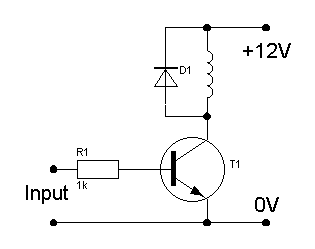
\includegraphics[width=6cm]{transistori_pics/rele.png} % http://www.electro-tech-online.com/electronic-projects-design-ideas-reviews/95934-comparator-not-working-transistor.html
\end{center}

Suojadiodin tarkoitus on mahdollistaa kelan (releen käämin) energian purkautuminen hallitusti, kun transistori katkaisee virran.
 }


 \frame{
 \frametitle{Darlington-kytkentä}
Jos virtavahvistusta tarvitaan paljon, transistorit voidaan kytkeä niin, että ensimmäisen transistorin emitterivirta syötetään toisen transistorin kannalle. Piiriä kutsutaan Darlington-kytkennäksi.
\begin{center}
\begin{picture}(100,100)(0,0)

\npn{0,50}{}
\npn{50,25}{}

\hln{50,75}{50}
\vln{100,50}{50}
%\vln{100,100}{25}

\out{0,50}
\out{100,-25}
\out{100,100}
\vln{100,-25}{25}

\di{100,90}{I_1}
\ri{10,50}{I_2}

\end{picture}

\end{center}
 }

% TODO: Kerro Darlingtonin ja Sziklain eroista ja miksi ko. kytkentöjä käytetään.
% Ks. myös http://www.inner-magazines.com/news/50/66/60-Years-of-Audio-Transistors/

\frame{
\frametitle{Esimerkki: Sziklai-kytkentä}
\begin{center}
\begin{picture}(100,100)(0,0)

\npn{0,50}{}
\pnpc{50,75}{}

\hln{50,25}{50}
\vln{100,0}{50}
\vln{100,100}{25}

\out{0,50}
\out{100,0}
\out{100,125}

\di{100,115}{I_1}
\ri{10,50}{I_2}

\end{picture}

\end{center}
Laske koko piirin virtavahvistus $\beta_{\rm kok}=\frac{I_1}{I_2}$. Molemmilla transistoreilla on sama virtavahvistus $\beta$ (ei lukuarvoa).

}


\frame{
\frametitle{Esimerkki: Sziklai-kytkentä}
\begin{center}
\begin{picture}(100,100)(0,0)

\npn{0,50}{}
\pnpc{50,75}{}

\hln{50,25}{50}
\vln{100,0}{50}
\vln{100,100}{25}

\out{0,50}
\out{100,0}
\out{100,125}

\di{100,115}{I_1=\beta^2I_2+\beta I_2}
\ri{10,50}{I_2}

\li{55,75}{\beta I_2}
\di{100,40}{\beta\beta I_2=\beta^2I_2}

\end{picture}

\end{center}
\[
\beta_{\rm kok}=\frac{I_1}{I_2}=\frac{\beta^2I_2+\beta I_2}{I_2}=\beta^2 + \beta
\]
}


\frame{
\frametitle{Käytännön bipolaaritransistorit}
Valintaan vaikuttavat muun muassa
\begin{itemize}
\item Virtavahvistus
\item Suurin sallittu kollektorivirta
\item Kollektori-emitteri -liitoksen jännitteenkesto
\item Yksikkövahvistuksen rajataajuus $f_{\rm T}$
\end{itemize}
}

\frame{
\frametitle{Virtavahvistus}
\begin{itemize}
\item Transistorin valmistaja takaa yleensä jonkin vähimmäisvirtavahvistuksen tietyllä kollektorivirralla.
\item Toleranssit ovat suuria.
\item (Muuten) samaa transistoria myydään usein eri virtavahvistuksilla, esim. BC547A, BC547B ja BC547C.
\end{itemize}
}

\frame{
\frametitle{Suurin sallittu kollektorivirta ja SOA}
\begin{itemize}
\item Kuumenemisteho rajoittaa transistorin virrankestoa.
\item SOA = Safe Operating Area on valmistajan ilmoittama alue sallituille kollektori-emitteri -jännitteille ja kollektorivirroille.
\end{itemize}
}

\frame{
\frametitle{Jännitteenkesto}
\begin{itemize}
\item Jos kollektorin ja emitterin välinen jännite on liian suuri, tapahtuu läpilyönti.
\end{itemize}
}

\frame{
\frametitle{Hajakapasitanssit ja yksikkövahvistuksen rajataajuus}
\begin{itemize}
\item Transistorin sisäiset kapasitanssit saavat aikaan sen, että taajuuden kasvaessa vahvistuskerroin pienenee.
\item Valmistaja ilmoittaa usein yksikkövahvistuksen rajataajuuden $f_{\rm T}$ eli taajuuden, jolla $\beta$ on laskenut
arvoon 1.
\end{itemize}
}

\frame{
\frametitle{Early-jännite}
\begin{itemize}
\item Perinteisessä transistorimallissa virtavahvistuskerroin oletetaan vakioksi. Todellisuudessa kollektorivirta kasvaa,
kun kollektorin ja emitterin välinen jännite kasvaa.
\item Ominaiskäyrille piirretyt jatkeet leikkaavat pisteessä $-U_{\rm A}$, missä $U_{\rm A}$ on Early-jännite.
\item Tätä voidaan mallintaa kollektorin ja emitterin välille piirrettävällä vastuksella
\[
r_0=\frac{|U_{\rm A}|+|U_{\rm CE}|}{I_{\rm C}}\approx \frac{|U_{\rm A}|}{I_{\rm C}}
\]
\end{itemize}
}

\frame{
\frametitle{Tasasuuntaajat ja regulaattorit}
\begin{itemize}
\item Käytännössä kaikki elektroniikkalaitteet vaativat syöttöjännitteeksi tasajännitteen.
\item Laitetta, joka muuttaa sähköverkosta saatavan vaihtosähkön elektroniikkalaitteelle sopivaksi
tasasähköksi, kutsutaan verkkolaitteeksi tai teholähteeksi. Arkikielessä käytetään myös termejä virtalähde, poweri,
adapteri tai muuntaja.
\item Teholähde voidaan toteuttaa kahdella päätavalla: lineaarisena teholähteenä tai hakkuriteholähteenä.
\end{itemize}
}

\frame{
\frametitle{Teholähteen ominaisuudet}
\begin{itemize}
\item Nimellisjännite
\item Maksimivirta/teho
\item Hurinajännite
\end{itemize}
}

\frame{
\frametitle{Lineaarinen teholähde}
Lineaarisessa teholähteessä
\begin{itemize}
\item verkkojännite alennetaan ensin verkkomuuntajalla. 
\item Seuraavaksi jännite tasasuunnataan (yleensä) diodisillalla.
\item Diodisillalta saatava sykkivä tasajännite suodatetaan tasaisemmaksi kondensaattorilla.
\item Jos tarvitaan erittäin stabiilia tasajännitettä, käytetään lisäksi regulaattoria, joka "leikkaa"\ jännitteen vaihtelut pois.
\end{itemize}
Verkkolaitteessa on tavallisesti myös sulake muuntajan ensiöpuolella.
}

\frame{
\frametitle{Muuntaja}
\begin{itemize}
\item Kaksi kelaa, joiden välillä keskinäisinduktanssia.
\item Toiseen kelaan syötetty muuttuva virta aikaansaa toiseen kelaan muuttuvan jännitteen.
\item Ensiö- ja toisiojännitteiden suhde eli muuntosuhde määräytyy suoraan käämien kierroslukujen perusteella.
\end{itemize}
}

\frame{
\frametitle{Tasasuuntaus}
\begin{itemize}
\item Muuntajalta saatava sinimuotoinen vaihtojännite tasasuunnataan sykkiväksi tasajännitteeksi.
\end{itemize}
}

\frame{
\frametitle{Suodatuskondensaattori}
\begin{itemize}
\item Sykkivä tasajännite ei kelpaa (harvinaisia poikkeuksia lukuunottamatta) sellaisenaan laitteen syöttöjännitteeksi.
\item Käyttämällä suodatuskondensaattoria voidaan sykkivää tasajännitettä tasoittaa vähemmän sykkiväksi.
\item Kondensaattori luovuttaa virtaa kuormalle, kun tasasuuntaajalta tuleva jännite laskee.
\item Suodatetun tasajännitteen vaihtelua kutsutaan hurinajännitteeksi (muita nimiä: ripple (engl.), rippeli, brummi).
\end{itemize}
}


\frame{
\frametitle{(Lineaarinen) regulaattori}
\begin{itemize}
\item Regulaattori leikkaa hurinajännitteen pois.
\item Esimerkiksi jos 5 voltin regulaattorille syötetään välillä 9--12 V vaihtelevaa tasajännitettä, regulaattori pitää lähtöjännitteen jatkuvasti viidessä voltissa.
\item Lineaarinen regulaattori koostuu säätöpiiristä ja tehotransistorista. Säätöpiiri vertaa lähtöjännitettä sisäiseen vertailujännitteeseen ja säätää transistorin johtavuutta niin, että lähtöjännite pysyy vakiona, vaikka kuorman virrankulutus ja tulojännite vaihtelisivat.
\item Tunnetuin regulaattorisarja on 78xx. Kaksi viimeistä numeroa kertovat jännitteen, esimerkiksi 7805 reguloi lähtöjännitteen viiteen volttiin.
\item Regulaattori vaatii tietyn minimijännitteen, jotta se toimii normaalisti. 78xx-sarjalla tämä on yleensä 2\ldots 2,5 volttia yli nimellisjännitteen. Lopullinen arvo kannattaa varmistaa valmistajan datalehdestä.
\item Regulaattoreita on saatavilla myös säädettävänä, esimerkiksi LM317.
\end{itemize}
}


\frame{
\frametitle{Esimerkki lineaarisesta teholähteestä}
\begin{center}
\begin{picture}(280,150)(0,-40)

\out{0,0}
\out{0,50}
\hln{0,0}{50}
\hln{0,50}{50}
\txt{0,25}{230\V\ 50\Hz}

\vl{50,0}{}
\vlr{75,-25}{}
\vlr{75,25}{}
\put(59,0){\line(0,1){50}}
\put(62,0){\line(0,1){50}}
\put(65,0){\line(0,1){50}}

\rd{75,-25}{D_2}
\rd{75,75}{D_1}

\vcj{125,25}
\vln{125,-25}{45}
\vln{125,30}{45}

\hln{75,25}{200}

\vc{150,25}{C_1}
\vc{235,25}{C_2}
\vz{275,25}{R_\mathrm{L}}

\put(175,60){\framebox(30,30){}}
\vln{190,25}{35}
\hgp{190,25}
\cn{190,25}
\stx{190,100}{Regulaattori}

\hln{125,75}{50}
\hln{205,75}{70}

\stx{169,80}{$\Uin$}
\stx{215,80}{$\Uout$}

\end{picture}
\end{center}
Koska muuntajassa on keskiulosotto, voidaan kokoaaltotasasuuntaus toteuttaa kahdella diodilla.
}

\frame{
\frametitle{Suodatuskondensaattorin mitoitus}
\begin{itemize}
\item Suodatuskondensaattori $C_1$ on valittava sellaiseksi, että regulaattorin tulojännite ei laske alle sallitun minimin.
\item Mitä suurempi kondensaattori, sitä pienempi on hurinajännite.
\item Jos kuorman ottama virta oletetaan vakioksi ja oletetaan, että purkautuminen kestää 10 millisekuntia, niin kondensaattorin vähimmäiskoko on
\[
C=\frac{I\cdot 10\, {\rm ms}}{\Delta U},
\]
missä $I$ on kuorman ja regulaattorin ottama virta ja $\Delta U$ on regulaattorille tulevan maksimijännitteen ja regulaattorin vaatiman minimijännitteen erotus.
\end{itemize}
}

\frame{
\frametitle{Kondensaattorin mitoittaminen: tarkempi tapa}
Kondensaattorin ei tarvitse antaa virtaa koko 10 millisekunnin jakson ajan. Voidaan helposti osoittaa, että seuraava nouseva jakso saavuttaa purkautuvan kondensaattorin jännitteen vaihekulman $\phi$ kuluttua, jolloin kondensaattorin minimikoko voidaan laskea:
\begin{itemize}
\item $C=\frac{I\Delta t}{\Delta U}$
\item $\Delta t=\frac{\phi}{360^\circ}\frac{1}{f_{\rm verkko}}$
\item $\phi=90^\circ+\arcsin \frac{U_{\rm min}+U_{\rm diodi(t)}}{U_{\rm max}+U_{\rm diodi(t)}}$.
\end{itemize}
Kaavassa $U_{\rm min}$ ja $U_{\rm max}$ ovat regulaattorille tuleva minimi- ja maksimijännite.
}




\frame{
\frametitle{Kanavatransistorit}
\begin{itemize}
\item Tyypit MOSFET ja JFET
\item Kalvoilla käsitellään N-kanava JFET ja N-kanavainen avaustyyppinen MOSFET
\end{itemize}
\begin{center}
\begin{picture}(150,50)(0,0)

\njfet{0,0}{\rm JFET}
\benmos{100,0}{\rm MOSFET}
\vln{150,-3}{8}
\end{picture}
\end{center}
}

\frame{
\frametitle{n-kanava-JFET}
\begin{itemize}
\item Hilalla estosuuntainen diodiliitos -- ei kulje virtaa.
\item Hilan ja lähteen välisellä jännitteellä säädellään nieluvirtaa
\item Jos $U_{\rm GS}=0\V$, niin $I_{\rm D}=I_{\rm DSS}$, missä $I_{\rm DSS}$ on komponenttikohtainen vakio
\item Jos $U_{\rm GS}=U_{\rm P}$, niin $I_{\rm D}=0$. $U_{\rm P}$ on komponenttikohtainen vakio, ja se on negatiivinen,
esimerkiksi $-3$ volttia.
\item Näiden ääripäiden välillä $I_{\rm D}=I_{\rm DSS}(1-\frac{U_{\rm GS}}{U_{\rm P}})^2$ kun $\ U_{\rm DS}\ge U_{\rm GS}-U_{P}$
\end{itemize}
\begin{picture}(50,50)(-100,-20)

\njfet{0,0}{\rm JFET}
\txt{-10,0}{\rm G}
\txt{55,25}{\rm D}
\txt{55,-15}{\rm S}

\end{picture}
}

\frame{
\frametitle{MOSFET}
\begin{itemize}
\item Kuten JFET: $I_{\rm D}=0$ ja $U_{\rm GS}$ säätelee nieluvirtaa
\item Hilajännitteen oltava $>U_{\rm T}$, jotta virta kulkisi
\item $I_{\rm D}=K(U_{\rm GS}-U_{T})^2, \mbox{kun}\ U_{\rm GS} \ge U_{T}\ \mbox{ja}\ U_{\rm DS}\ge U_{\rm GS}-U_{T}$
\item $U_{\rm T}$ ja $K$ ovat komponenttikohtaisia vakioita
\item Jos hilajännite hyvin suuri (luokkaa $>10 \V$), kanava aukeaa täysin ja näyttää pieneltä resistanssilta
$R_{\rm DS on}$
\end{itemize}

\begin{picture}(50,50)(-100,-20)

%\njfet{0,0}{\rm JFET}
\txt{-10,0}{\rm G}
\txt{55,25}{\rm D}
\txt{55,-15}{\rm S}

\benmos{0,0}{\rm MOSFET}
\vln{50,-3}{8}

\end{picture}
}


\frame{
\frametitle{Käytännön vastukset}

\begin{itemize}
\item Massavastukset
\item Hiilikalvovastukset
\item Metallikalvovastukset
\item Lankavastukset
\end{itemize}
Mikropiireissä vastukset vievät paljon tilaa $\to$ pyritään korvaamaan muilla komponenteilla.
}

\frame{
\frametitle{Ominaisuudet}
\begin{itemize}
\item Nimellisarvo
\item Tehonkesto
\item Toleranssi
\item Lämpötilariippuvuus
\end{itemize}
}

\frame{
\frametitle{E-sarjat}
\begin{itemize}
\item Komponentteja ei ole käytännössä järkevää (eikä mahdollistakaan) valmistaa jokaista mahdollista lukuarvoa.
\item Yleinen sarja on E12: 10, 12, 15, 18, 22, 27, 33, 39, 47, 56, 68, 82

\end{itemize}
}

\frame{
\frametitle{Värikoodit}
\begin{itemize}
\item Tehovastuksissa nimellisarvo ja tehonkesto on merkitty numeroin vastuksen kylkeen.
\item Pienillä vastuksilla arvo on värikoodattu.
\item Välillä on hankala tietää, kummasta päästä lukeminen aloitetaan ja mitkä arvot kuuluvat lukuarvoon.
\end{itemize}
}

\frame{
\frametitle{Loisilmiöt}
\begin{itemize}
\item Ideaalista vastusta ei ole olemassakaan.
\item Tarkka mallintaminen vaikeaa.
\item Rinnakkaiskapasitanssi (pikofaradeja tai vähemmän).
\item Sarjainduktanssi: kymmeniä nano- tai korkeintaan muutama mikrohenryjä.
\item Kohina (mikrovoltteja).
\end{itemize}
}

\frame{
\frametitle{Erikoisvastuksia}
\begin{itemize}
\item Säätövastus eli potentiometri.
\item VDR
\item NTC ja PTC
\end{itemize}
}

\frame{
\frametitle{Kela}
\begin{itemize}
\item Ideaalisen kelan toiminta noudattaa yhtälöä
\[
u=L\frac{{\rm d}i}{{\rm d}t}
\]
\item Kela eli käämi eli solenoidi valmistetaan kiertämällä kuparilankaa sydämen ympärille.
\item Sydän voi olla ilmaa, muovia tai magneettista materiaalia.
\item Sydän on yleensä lieriön muotoinen (lieriökäämi) tai toruksen muotoinen (toroidi- eli rengaskäämi).
\item Kelaa, jonka tarkoitus piirissä on virran rajoittaminen, kutsutaan kuristimeksi.  
\item Kelojen käyttöä pyritään yleensä välttämään elektroniikkasuunnittelussa.
\end{itemize}
}

\frame{
\frametitle{Miksi kelojen käyttöä pyritään välttämään}
\begin{itemize}
\item Keloja on kömpelö valmistaa.
\item Kelat vievät paljon tilaa.
\item Kelat aiheuttavat ympärilleen magneettikentän.
\end{itemize}
}

\frame{
\frametitle{Milloin kelojen käyttö on käytännössä pakollista}
\begin{itemize}
\item Hakkuriteholähteet
\item Releet
\item Suurtaajuuslaitteissa kelaa ei voi aina korvata muilla ratkaisuilla.
\end{itemize}
}

\frame{
\frametitle{Käytännön kelan ominaisuudet}
\begin{itemize}
\item Induktanssi toleransseineen
\item Maksimi virrankesto
\item Sarjaresistanssi
\end{itemize}
}

\frame{
\frametitle{Sydänmateriaalin vaikutus}
\begin{itemize}
\item Kelan induktanssi riippuu sydänmateriaalin permeabiliteetista $\mu=\mu_0\mu_{\rm r}$.
\item Diamagneettisilla aineilla (mm. jalometallit) $\mu_{\rm r}$ on aavistuksen verran ykköstä pienempi, paramagneettisilla aineilla kuten ilmalla tai alumiinilla aavistuksen verran ykköstä suurempi.
\item Ferromagneettisilla aineilla $\mu_{\rm r}$ on useita satoja tai jopa yli miljoona.
\end{itemize}
}

\frame{
\frametitle{Pyörrevirtahäviöt}
\begin{itemize}
\item Jos kelan sydän on sähköäjohtavaa materiaalia, sinne indusoituu pyörrevirtoja.
\item Pyörrevirrat aiheuttavat lämpöhäviöitä.
\item Ferriitit ($\rm XOFe_2O_3$) sopivat hyvin sydänmateriaaliksi: niillä on korkea $\mu_{\rm r}$
mutta matala sähkönjohtavuus, jolloin pyörrevirtahäviöt jäävät pieniksi.
\item Yksi tapa vähentää pyörrevirtahäviöitä on käyttää levypakkasydäntä, joka koostuu toisistaan eristetyistä rautalevyistä. Tätä ratkaisua käytetää muun muassa verkkomuuntajissa.
\end{itemize}
}

\frame{
\frametitle{Erilaisia keloja}
\begin{center}
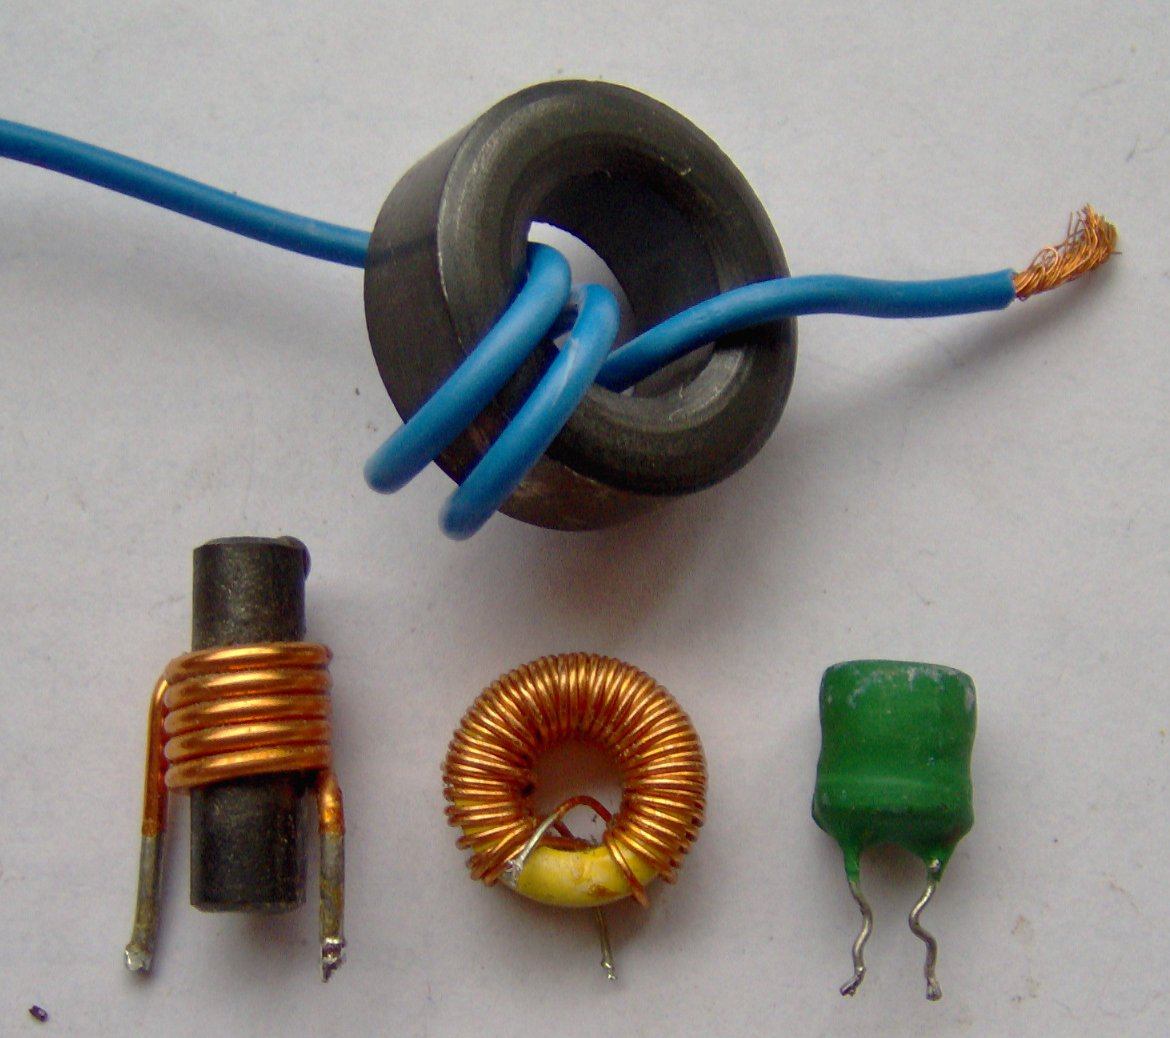
\includegraphics[height=70mm]{kelat_pics/Electronic_component_inductors.jpg}
\end{center}
\tiny \url{http://commons.wikimedia.org/wiki/File:Electronic_component_inductors.jpg} 
}


\frame{
\frametitle{Maxwellin yhtälöt}
Maxwellin yhtälöiden käsittely vaatii yliopistomatematiikkaa. Täällä käydään läpi
vain yhtälöiden merkitys. Maxwellin yhtälöitä on 4:
\begin{itemize}
\item $\nabla \times \vec E=-\frac{{\rm d}B}{{\rm d}t}$ {\bf Faradayn induktiolaki}. Muuttuva magneettikenttä saa aikaan sähkökentän.
\item $\nabla \cdot \vec D=\rho$ {\bf Gaussin laki}. Sähkövaraus $\rho$ saa aikaan sähkökentän.
\item $\nabla \times \vec H=\vec J + \frac{{\rm d}D}{{\rm d}t}$ {\bf Lävistyslaki}. Sähkövirta aikaansaa magneettikentän.
\item $\nabla \cdot \vec B=0$ {\bf Gaussin laki magneettikentille}. Magneettikenttäviivat ovat aina sulkeutuvia eli suljetun pinnan läpi
magneettivuo on nolla.
\end{itemize}
{Maxwellin yhtälöt ovat koko sähkötekniikan perusta.} Niitä ei voi "perustella", ne ovat kokeellisesti
havaittu luonnonlaki, kuten vaikkapa mekaniikasta tuttu $F=ma$.
}


\frame{
\frametitle{Johtimen magneettikenttä}
Maxwellin yhtälöistä voidaan laskea, että suorassa johtimessa kulkeva virta $I$ aikaansaa
magneettikentän, jonka voimakkuus etäisyydellä r johtimesta on $H=\frac{I}{2\pi r}$.
Magneettikenttäviivat kiertävät johdinta.
}

\frame{
\frametitle{Kelan toiminta}
Koska
\begin{itemize}
\item muuttuva magneettikenttä saa aikaan jännitteen johtimeen
\item johtimessa kulkeva virta saa aikaan magneettikentän ja johtimessa kulkeva
muuttuva virta, 
\end{itemize}
niin muuttuva virta johtimessa saa johtimeen aikaan jännitteen joka vastustaa virran muutosta.
Tähän perustuu komponentti nimeltä kela, johon olemme jo tutustuneetkin. Kiertämällä
johdin käämiksi (siis kelaksi) tämä pyrkimys vastustaa virran muutoksia (=induktanssi) kasvaa.
}

\frame{
\frametitle{Muuntajan toiminta}
Kytkemällä kaksi kelaa siten, että toisen magneettikenttä kulkee toisen kelan läpi, syntyy
muuntaja. Tämä voi olla myös ei-toivottu ilmiö. Piirilevyllä lähekkäin kulkevien johtimien
magneettikentät vaikuttavat toisiin johtimiin; tätä ilmiötä kutsutaan {\bf ylikuulumiseksi}.
}



%Seuraavat kaksi kalvoa pöllitty S2010 EMC-kalvoilta ja vähän muokattu

\frame{
\frametitle{Magneettivuo}
\begin{itemize}
\item Magneettivuon tiheys $B$ riippuu magneettikentän voimakkuudesta $H$ ja väliaineen permeabiliteetista $\mu$
\[
B=\mu H
\]
\item Vuontiheyden yksikkö on tesla (T). Puhekielessä magneettikentän voimakkuus ja magneettivuon tiheys menevät usein sekaisin (esim. mitataan vuontiheyttä ja puhutaan kentänvoimakkuudesta).
\item Pinta-alan $A$ läpi kulkeva magneettivuo $\phi$ on
\[
\phi = \int_A \vec{B}\cdot {\rm d} \vec{A}
\]
\end{itemize}
}


\frame{
\frametitle{Sähkömagneettinen induktio}
\begin{itemize}
\item Faradayn lain mukaan muuttuva magneettivuo $\phi$ indusoi käämiin jännitteen, jonka suuruus on
\[
e=-\frac{{\rm d}\phi }{{\rm d}t}
\]
\item Koska vuontiheys on sitä suurempi mitä suurempi on permeabiliteetti ja vuontiheyden muutosnopeus vaikuttaa induktiojännitteeseen, on kelan induktanssi suoraan verrannollinen sydämen
suhteelliseen permeabiliteettiin $\mu_{\rm r}$.
\end{itemize}
}


\frame{
\frametitle{Hystereesi}
\begin{itemize}
\item Ferromagneettisilla aineilla $\mu_{\rm r}$ on hyvin suuri, mutta myös voimakkaasti riippuvainen magneettikentän voimakkuudesta!
\item Suurilla kentänvoimakkuuksilla materiaali {\em kyllästyy} ja $\mu_{\rm r}$ pienenee mitä suuremmaksi magneettikentän voimakkuus kasvaa.
\end{itemize}
}

\frame{
\frametitle{Hystereesi}
\begin{center}
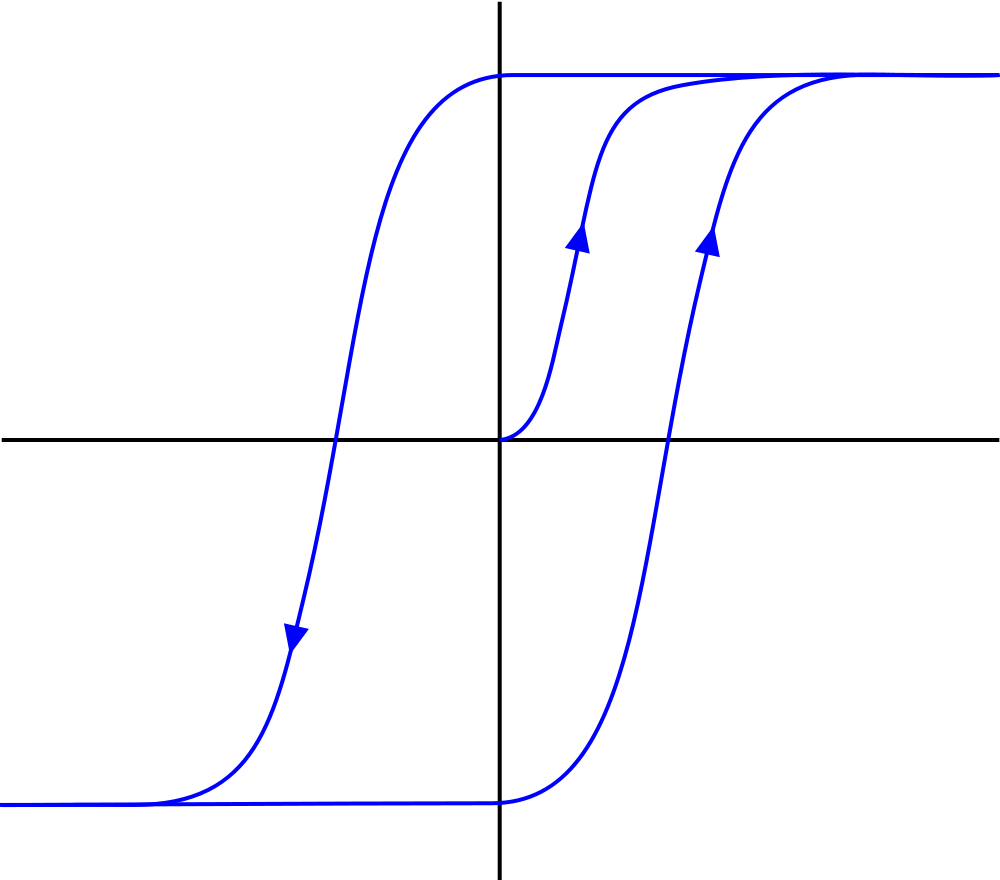
\includegraphics[height=70mm]{kelat_pics/1000px-Hysteresiscurve.png}
\end{center}
\tiny \url{http://commons.wikimedia.org/wiki/File:Hysteresiscurve.svg} 

}

\frame{
\frametitle{Kondensaattori}
\begin{itemize}
\item Ideaalisen kondensaattorin toiminta noudattaa yhtälöä
\[
i=C\frac{{\rm d}u}{{\rm d}t}
\]
\item Yksinkertaisen tasokondensaattorin kapasitanssi riippuu levyjen pinta-alasta, niiden välisestä etäisyydestä sekä eristeaineen permittiivisyydestä:
\[
C=\epsilon_0\epsilon_{\rm r}\frac{A}{d}
\]
\item Kondensaattori valmistetaan pinoamalla ohuita levyjä eristeineen päällekkäin, ja kiertämällä näin saatu levypino rullalle.
\item Eristettä ohentamalla kapasitanssi kasvaa, mutta jännitteenkesto pienenee.
\end{itemize}
}


\frame{
\frametitle{Käytännön kondensaattorien ominaisuudet}
\begin{itemize}
\item Kapasitanssi toleransseineen
\item Jännitteenkesto
\item Sarjaresistanssi
\end{itemize}
}

\frame{
\frametitle{Kondensaattorien merkinnät}
\begin{itemize}
\item Aikaisemmin käytettiin värikoodeja.
\item Suuriin kondensaattoreihin kapasitanssi merkitään yleensä selkokielellä.
\item Hyvin yleinen on merkintätapa, jossa on kolme numeroa ja yksi kirjain. Kaksi ensimmäistä numeroa
kertoo kapasitanssin pikofaradeina, kolmas nollien lukumäärän ja kirjain kertoo toleranssin (K = $\pm 10\%$, M = $\pm 20 \%$ ja Z = $-20\ldots +80 \%$).
\item Esimerkiksi 474M on 470000 pF eli 470 nF kondensaattori, jonka toleranssi on $\pm 20 \%$. 
\item Merkintä 100V tarkoittaa yksinkertaisesti, että kondensaattorin jännitteenkesto on 100 volttia. 
\end{itemize}
}

\frame{
\frametitle{Päätyypit}
\begin{itemize}
\item Keraamiset kondensaattorit
\item Muovikondensaattorit
\item Elektrolyyttikondensaattorit ("tavallinen" ja tantaalikondensaattori)
\end{itemize}
}

\frame{
\frametitle{Elektrolyyttikondensaattorien kytkeminen}
\begin{itemize}
\item Elektrolyyttikondensaattoreissa eristekerros muodostuu kemiallisen reaktion seurauksena
\item Jos elektrolyyttikondensaattori (= "elko") kytketään väärin päin piiriin, eristekerrosta ei muodostu ja kondensaattori käyttäytyy kuin matalaresistanssinen vastus ja yleensä tuhoutuu.
\item Huom! Virta saa kulkea välillä myös väärään suuntaan. Pääasia on, että kun laite kytketään päälle, kondensaattorissa kulkee ensin virta oikeaan suuntaan.
\end{itemize}
}

\frame{
\frametitle{Sovelluksia}
\begin{itemize}
\item Energiavarasto
\item Suodatus signaalinkäsittelyssä
\item Loistehon kompensointi ja tehosovitus
\item Läheisyysanturi
\item Kosketusnäytöt
\end{itemize}
}

\frame{
\frametitle{Tehoelektroniikan komponentit}
Tehoelektroniikka = käytetään sähköä suurtehosovelluksissa elektronisesti ohjaten. Tärkeitä komponentteja
\begin{itemize}
\item IGBT eli eristehilabipolaaritransistori
\item SCR-tyristori
\item GTO-tyristori
\item Triac ja diac
\end{itemize}
}

\frame{
\frametitle{IGBT eli eristehilabipolaaritransistori}
\begin{itemize}
\item Kytkinkäyttöön suunniteltu jänniteohjattu komponentti.
\item Uudehkoa tekniikkaa (kehitetty 1980-luvulla).
\item Suurilla taajuuksilla MOSFET on edelleen yleisesti käytetty.
\item Suurilla tehoilla käytetään perinteisiä tyristorikomponentteja.
\end{itemize}
}

\frame{
\frametitle{Tyristorikomponentit}
\begin{itemize}
\item SCR-tyristori
\item GTO-tyristori
\item Triac
\item Diac
\end{itemize}
}

\frame{
\frametitle{SCR-tyristori}
\begin{itemize}
\item Neljästä puolijohdekerroksesta valmistettu "perinteinen"\ tyristori.
\item Toiminta lyhyesti: hilalle annettu jännitepulssi saa tyristorin johtamaan.
\item Tyristori johtaa niin kauan, kun virta anodilta katodille on riittävän suuri.
\item SCR-tyristori lakkaa johtamasta eli {\em sammuu} vasta, kun pitovirta alitetaan.
\end{itemize}
}

\frame{
\frametitle{GTO-tyristori}
\begin{itemize}
\item Kuten SCR-tyristori, mutta se voidaan sammuttaa antamalla hilalle negatiivinen jännitepulssi.
\end{itemize}
}

\frame{
\frametitle{Triac}
\begin{itemize}
\item Toimii kuten kaksi rinnakkain mutta vastakkaisiin suuntiin kytkettyä tyristoria.
\item Käytetään vaihtosähkötehon säätöön.
\end{itemize}
}

\frame{
\frametitle{Diac}
\begin{itemize}
\item Diacissa
\item Diacia käytetään Triacin liipaisuun.
\end{itemize}
}

\frame{
\frametitle{Tehonsäätö}
\begin{itemize}
\item Tyristorikomponenteilla tehonsäätö perustuu vaihesäätöön.
\item Tyristori/Triac kytketään johtamaan, kun siniaallon puolijakso on saavuttanut tietyn vaihekulman.
\end{itemize}
}

\frame{
\frametitle{Komponenttiesimerkkejä}
\begin{itemize}
\item Teho-MOSFET BUZ11
\item Tyristori TIC106
\item Triac TIC226D
\item Diac DB3
\item IGBT IRG4BC30U
\end{itemize}
}


\frame{
\frametitle{Ei-portti}
\begin{center}
\begin{picture}(100,50)(0,0)
\hln{-10,15}{10}
\hnot{0,0}
\end{picture}
\end{center}
Jos tulo on 0, lähtö on 1. Jos tulo on 1, lähtö on 0.
}

\frame{
\frametitle{Ja-portti}
\begin{center}
\begin{picture}(100,50)(0,0)
\hand{0,0}
\hln{-10,0}{10}
\hln{-10,20}{10}

\end{picture}
\end{center}
Lähtö on 1 jos ja vain jos kaikki tulot ovat 1, muuten lähtö on 0.
}


\frame{
\frametitle{Tai-portti}
\begin{center}
\begin{picture}(100,50)(0,0)
\hor{0,0}
\hln{-10,0}{10}
\hln{-10,20}{10}

\end{picture}
\end{center}
Lähtö on 0 jos ja vain jos kaikki tulot ovat 0, muuten lähtö on 1.
}

\frame{
\frametitle{Yksinomainen tai -portti (XOR)}
\begin{center}
\begin{picture}(100,50)(0,0)
\hxor{0,0}
\hln{-10,0}{10}
\hln{-10,20}{10}

\end{picture}
\end{center}
Lähtö on 1 jos jompikumpi (mutta ei molemmat) tuloista on 1, muuten lähtö on 0.
}

\frame{
\frametitle{Esimerkki}
Suunnittele logiikkaporttipiiri, joka antaa lähtösignaalin 1 (antaa äänimerkin), jos auton avaimet eivät ole virtalukossa,
ovi on auki ja ajovalot ovat päällä. Tulosignaalit ovat:\\
$A$ = "Avaimet ovat virtalukossa"\\
$B$ = "Ovi on auki"\\
$C$ = "Ajovalot ovat päällä"\\

{\bf Yksi esimerkki toimivasta ratkaisusta}:
\begin{center}
\begin{picture}(100,100)(0,0)
\hnot{20,50}
\vln{50,20}{43}
\hln{50,20}{20}

\hand{70,0}
\txt{0,60}{A}
\txt{0,30}{B}
\txt{0,0}{C}
\hln{0,60}{20}

\hln{0,0}{70}
\hln{0,30}{30}
\vln{30,10}{20}
\hln{30,10}{40}


\end{picture}
\end{center}


}
 \frame{
 \frametitle{Lukujärjestelmät}
 \begin{itemize}
\item Kymmenjärjestelmä
 \item Binaarijärjestelmä
\item Heksadesimaalijärjestelmä
\item Muunnokset järjestelmästä toiseen
 \end{itemize}
 }

 \frame{
 \frametitle{Kymmenjärjestelmä}
 \begin{itemize}
\item Ihmisten käyttämä numerojärjestelmä on kymmenjärjestelmä eli lukujärjestelmän kantaluku on 10. 
\item Numeromerkkejä on käytössä 10 kappaletta (0--9).
\item Kymmenjärjestelmä on paikkapohjainen eli positiojärjestelmä. Eniten merkitsevä numero on vasemmalla, ja vähiten merkitsevä oikealla.
\item Oikeanpuolimmainen numeromerkki kertoo kantaluvun nollannen potenssin kertoimen, seuraava ensimmäisen potenssin kertoimen ja niin edelleen.
\item Kun halutaan korostaa, mistä lukujärjestelmästä on kysymys, kantaluku merkitään oikeaan alaindeksiin.
 \end{itemize}
\[
123_{10}=1\cdot 10^2 + 2 \cdot 10^1 + 3 \cdot 10^0
\]

 }

 \frame{
 \frametitle{Binaarijärjestelmä eli 2-järjestelmä}
 \begin{itemize}
\item Usein puhutaan binäärijärjestelmästä, koska se sopii suomalaiseen suuhun paremmin. Sanakirjat suosittelevat binaari-sanan käyttöä.
\item Binaarijärjestelmän kantaluku on 2.
\item 2-järjestelmää käytetään sen yksinkertaisuuden vuoksi digitaali- ja tietotekniikassa.
\item Numeromerkkejä on käytössä kaksi: 0 ja 1.
\[
1111011_2=123_{10}
\]
Muunnos binaarijärjestelmästä kymmenjärjestelmään on helppo: lasketaan vain kahden potenssit yhteen:
\[
1111011_2=1\cdot 2^6+1\cdot 2^5+1\cdot 2^4+1\cdot 2^3+0\cdot 2^2+1\cdot 2^1+1\cdot 2^0= 123_{10}
\] 
\end{itemize}
 }

 \frame{
 \frametitle{Muunnos kymmenjärjestelmästä binaarijärjestelmään}
Jaetaan toistuvasti luvulla 2, ja kirjataan jakojäännös ylös. Esimerkiksi 123 muunnetaan 2-järjestelmään näin:
\begin{eqnarray}
123 &=& 2\cdot 61 +\color{green}1\\
61 &=& 2\cdot 30 +\color{green}1\\
30 &=& 2\cdot 15 + \color{green}0\\
15 &=& 2\cdot 7 + \color{green}1\\
7 &=& 2\cdot 3 +\color{green}1\\
3 &=& 2\cdot 1 +\color{green}1\\
1 &=& 2\cdot 0 +\color{green}1
\end{eqnarray}
\[
123_{10}={\color{green}1111011}_2
\]
 }

 \frame{
 \frametitle{Heksadesimaalijärjestelmä}
 \begin{itemize}
\item Toinen tietokonetekniikassa käytössä oleva lukujärjestelmä on heksadesimaalijärjestelmä. Luvun kantaluku on 16.
\item Kymmenen pienintä numeromerkkiä ovat samat kuin kymmenjärjestelmässäkin. Sitten tulevat merkit A, B, C, D, E ja F.
\item Muunnokset tapahtuvat kuten kymmenjärjestelmästä binaarijärjestelmään (ja päin vastoin) muunnettaessa. Kantalukuna on 16, eli nyt jaetaan kuudellatoista.
 \end{itemize}
\begin{eqnarray}
123 &=& 16\cdot 7 +\color{green}11\\
7 &=& 16\cdot 0 +\color{green}7
\end{eqnarray}
\[
123_{10}={\color{green}7{\rm B}}_{16}
\]

 }

\frame{
 \frametitle{Muunnos binaarijärjestelmästä heksadesimaalijärjestelmään}
Kuusitoista on kahden potenssi, joten muunnos on helppo tehdä ryhmittelemällä. Muunnetaan $1111011_2$ heksadesimaalijärjestelmään:
\[
\underbrace{111}_{7_{10}=7_{16}}\qquad \underbrace{1011}_{11_{10}=\rm B}=7\rm B_{16}
\]

Periaate toimii helposti myös toiseen suuntaan muunnettaessa.
}

 \frame{
 \frametitle{Puolisummain}
\begin{center}
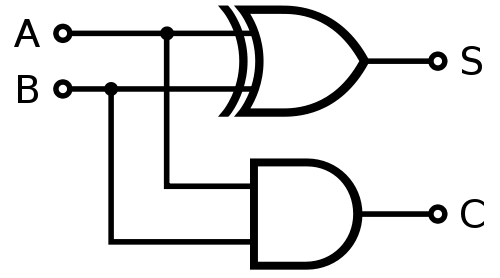
\includegraphics[width=5cm]{lukujarjestelmat_pics/500px-HalfAdder.png} % http://upload.wikimedia.org/wikipedia/commons/thumb/d/d9/Half_Adder.svg/500px-Half_Adder.svg.png
\end{center}


 \begin{itemize}
 \item Tuleva muistibitti (carry in) puuttuu. Soveltuu vain vähiten merkitsevän bitin yhteenlaskuun.
 \end{itemize}
 }

 \frame{
 \frametitle{Kokosummain} % http://upload.wikimedia.org/wikipedia/commons/thumb/a/aa/Full_Adder.svg/500px-Full_Adder.svg.png

\begin{center}
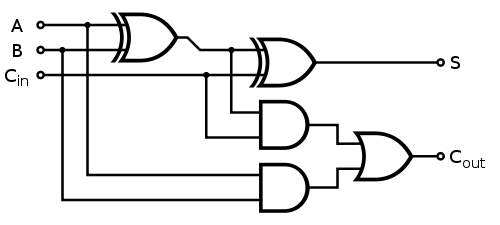
\includegraphics[width=10cm]{lukujarjestelmat_pics/500px-Full_Adder.png}
\end{center}
 \begin{itemize}
 \item Kokosummaimessa on tulo muistibitille, joten niitä voi ketjuttaa monta peräkkäin.
 \end{itemize}
 }


\frame{
 \frametitle{Termistöä}
\begin{description}
\item[bitti] Binaarijärjestelmän numeromerkki, lyhenne b.
\item[tavu] Kahdeksan bitin muodostama yksikkö, lyhenne B.
\item[kibitavu] $2^{10}$ bittiä eli 1024 tavua, lyhenne KiB.
\item[mebitavu] $2^{20}$ bittiä eli 1024 kibitavua eli 1 048 576 tavua, lyhenne MiB.
\end{description}
Bitti on englanniksi bit, tavu on englanniksi byte. Älä sotke niitä keskenään!
Ennen megatavu tarkoitti 1 048 576, mikä oli harhaanjohtavaa, koska kaikkialla muualla tekniikassa mega on $10^6$. Standardiuudistus vuonna 2010 selkiytti termistöä.
}

 \frame{
 \frametitle{Merkistöt}
 \begin{itemize}
 \item Vanhoissa tietokoneissa käytettiin 7-bittisiä merkistöjä, jolloin mahdollisia kirjanmerkkejä oli 128 (ASCII-standardi). 
\item 1990-luvulla siirryttiin 8-bittisiin merkistöihin (esim. ISO 8859-1), jolloin saatiin ääkköset mukaan (256 eri merkkiä). Haittapuolena oli, että eri kielissä on omat erikoismerkkinsä, jolloin tarvittiin useita eri merkistöjä. Jos merkistökoodaus oli valittu väärin, ääkköset näkyivät "pulunkakkoina".
\item 2000-luvulla on siirrytty UTF-8-merkistöön, jossa yhtä merkkiä koodataan neljällä tavulla. Tämä kattaa (käytännössä lähes) kaikki maailman kielten kirjoitusmerkit.
 \end{itemize}
 }

 \frame{
 \frametitle{Sekvenssipiirit}
 \begin{itemize}
 \item Logiikkaporttipiirit eli kombinaatiopiirit eivät ota huomioon aikaulottuvuutta: lähtöön vaikuttavat senhetkiset tulojen tilat.
\item Kombinaatiopiirien lisäksi tärkeitä digitaalipiirejä ovat {\bf sekvenssipiirit}. Sekvenssipiireissä lähdön tilaan vaikuttaa tulojen muuttumisen ajallinen järjestys sekä piirin senhetkinen tila.
 \end{itemize}
 }

 \frame{
 \frametitle{Dynaaminen tulo}
 \begin{itemize}
 \item Dynaaminen tulo vaikuttaa piirin toimintaan vain muutoshetkellä.
\item Eli "jotain tapahtuu"\ vain silloin, kun tulo muuttuu nollasta ykköseksi tai ykkösestä nollaksi.
\item Nollasta ykköseen -muutoksessa toimiva tulo on {\bf nousevalla reunalla toimiva} tulo. Sitä merkitään pienellä kolmiolla (alla vasemmalla).
\item Ykkösestä nollaan -muutoksessa toimiva tulo on {\bf laskevalla reunalla toimiva} tulo. Sitä merkitään pienellä kolmiolla, jonka edessä on pallo (alla oikealla).
 \end{itemize}
\begin{center}
\begin{picture}(50,50)(0,0)
\dff{0,0}
\jk{100,0}
\end{picture}
\end{center}

 }

 \frame{
 \frametitle{Kiikku vai veräjä?}
 \begin{itemize}
 \item Kiikku on sekvenssipiiri, jossa on kellotulo.
\item Veräjässä ei ole kellotuloa, vaan ohjaustuloissa tapahtuva muutos vaikuttaa piirin toimintaan välittömästi.
 \end{itemize}
 }

 \frame{
 \frametitle{SR-veräjä ja SR-kiikku}
 \begin{itemize}
\item Joskus kirjaimet ovat toisin päin (RS-kiikku/veräjä). Kyseessä on sama komponentti.
 \item Kun kellotuloon tuodaan positiivinen pulssi, lähdön $Q$ tila muuttuu ykköseksi jos $S$-tulon arvo on 1, ja nollaksi, jos $R$-tulon arvo on 1.
\item $S$=set, $R$=reset.
\item Jos molemmat tulot ovat nollia, tila ei muutu.
\item Tila, jossa $S$- että $R$-tuloihin syötetään ykkönen, on kielletty tila. Silloin piirin toimintaa ei ole määritelty (piiri voi toimia jotenkin arvaamattomasti).
\item SR-veräjä on kuten SR-kiikku, mutta erillinen kellotulo puuttuu, ja muutos tapahtuu välittömästi, kun tulojen tila muuttuu.
 \end{itemize}

\begin{center}
\begin{picture}(50,50)(0,0)
\sr{0,0}
\end{picture}
\end{center}
 }

 \frame{
 \frametitle{JK-kiikku}
 \begin{itemize}
 \item Melkein kuin SR-kiikku: J-tulo vastaa set-tuloa ja K-tulo reset-tuloa.
\item Parannus verrattuna SR-kiikkuun: JK-kiikussa ei ole "kiellettyä tilaa". Jos sekä $J$- että $K$-tulossa on arvo 1, niin lähtö vaihtaa tilaansa, kun kellopulssi tulee.
\item Monessa JK-kiikussa on lisäksi pakko-ohjaustulot $S$ ja $R$, joilla lähdön tilaa voidaan muuttaa kellosta riippumatta.
\item Kuvassa negatiivisella kellopulssin reunalla toimiva JK-kiikku.
 \end{itemize}
\begin{center}
\begin{picture}(50,50)(0,0)
\jk{0,0}
\txt{15,30}{J}
\txt{15,0}{K}

\txt{35,30}{Q}
\txt{35,0}{\bar{Q}}

\txt{25,52}{\bar{S}}
\txt{25,-25}{\bar{R}}

\end{picture}
\end{center}
 }

 \frame{
 \frametitle{D-kiikku}
 \begin{itemize}
 \item Toiminta hyvin yksinkertainen: lähtö $Q$ saa arvon $D$, kun kellopulssi tulee.
\item Kiikussa voi olla myös erilliset pakko-ohjaustulot ($S$ ja $R$).
 \end{itemize}
\begin{center}
\begin{picture}(50,50)(0,0)
\dff{0,0}
\txt{-10,30}{D}
\txt{-10,0}{clk}

\txt{35,30}{Q}
\txt{35,0}{\bar{Q}}

%\txt{25,52}{\bar{S}}
%\txt{25,-25}{\bar{R}}

\end{picture}
\end{center}
 }



\frame{
\frametitle{Suodattimet}
\begin{block}{Suodatin} % Määritelmä Silvonen sivu 405
= elektroninen piiri, jonka tehtävänä on vaikuttaa läpi menevän signaalin amplitudiin ja/tai vaiheeseen eri taajuuksilla eri tavoin.
\end{block}}

\frame{
\frametitle{Toteutustapoja}
\begin{itemize}
\item Suodatin voidaan toteuttaa joko analogisesti tai digitaalisesti
\item Analoginen suodatin on aktiivinen, jos toteutuksessa on käytetty vahvistimia. Pelkistä passiivikomponenteista (käytännössä vastus, kondensaattori ja kela) koottu suodatin on passiivinen suodatin.
\end{itemize}
}

\frame{
\frametitle{Suodatintyypit}
Tavallisimmat suodatintyypit ovat
\begin{itemize}
\item Alipäästösuodatin: vaimentaa korkeita taajuuksia, päästää läpi matalat taajuudet.
\item Ylipäästösuodatin: vaimentaa matalia taajuuksia, päästää läpi korkeat taajuudet.
\item Kaistanestosuodatin: päästää läpi korkeat ja matalat taajuudet, mutta vaimentaa tietyllä välillä olevia taajuuksia.
\item Kaistanpäästösuodatin: vaimentaa liian matalia ja liian korkeita taajuuksia, mutta päästää läpi tietyllä välillä olevat taajuudet.
\item Kokopäästösuodatin: vaimennus ei ole taajuusriippuvainen, ainoastaan vaihesiirto.
\end{itemize}
}

\frame{
\frametitle{Asteluku}
\begin{itemize}
\item Suodattimen asteluku = siirtofunktion $s$:n korkein potenssi.
\item Suodattimen asteluku analogisessa suodattimessa on yleensä sama kuin suodattimen kelojen ja kondensaattorien määrä.
\item Korkeampi asteluku merkitsee yleensä jyrkempää luiskaa päästökaistan ja estokaistan välillä.
\item Päästökaistan ja estokaistan välistä pistettä kutsutaan rajataajuudeksi (engl. cut-off frequency).
\end{itemize}
}


\frame{
\frametitle{1. asteen alipäästösuodatin}
\begin{itemize}
\item Yleinen muoto $F(s)=\frac{1}{s+1}$, tällöin ominaiskulmataajuus $\omega_0=1$.
\item Sijoittamalla $s\to \frac{s}{\omega_0}$ saadaan $F(s)=\frac{1}{\frac{s}{\omega_0}+1}$
\item Voidaan toteuttaa yksinkertaisella RC-piirillä, $F(s)=\frac{\Uout}{\Uin}=\frac{1}{RCs+1}$
\item Vertaamalla siirtofunktiota ja yleistä muotoa keskenään saadaan $\omega_0=\frac{1}{RC}$
\item Ominaistaajuudella $|F(s)|=\frac{1}{\sqrt{2}}$ ja vaihekulma $-45^\circ$
\end{itemize}

\begin{picture}(50,50)(-120,0)

\hz{0,50}{R}
\vc{50,0}{C}
\du{0,0}{\Uin}
\du{65,0}{\Uout}
\hln{0,0}{50}

\end{picture}



}

\frame{
\frametitle{2. asteen alipäästösuodatin}
\begin{itemize}
\item Yleinen muoto $\frac{1}{s^2+2Ds+1} \to \frac{1}{(\frac{s}{\omega_0})^2+2D\frac{s}{\omega_0}+1}$
\item Vaimennusvakio $D$ määrää vasteen muodon, $\omega_0$ paikan (kulma)taajuusakselilla
\item Voidaan toteuttaa esim. Sallen-Key -piirillä
\item {\bf Tärkeää!} Ominaiskulmataajuudella ei välttämättä $|F(s)|=\frac{1}{\sqrt{2}}$
\end{itemize}

}

\frame{
\frametitle{Butterworth-alipäästösuodattimen asteluvun vaikutus}
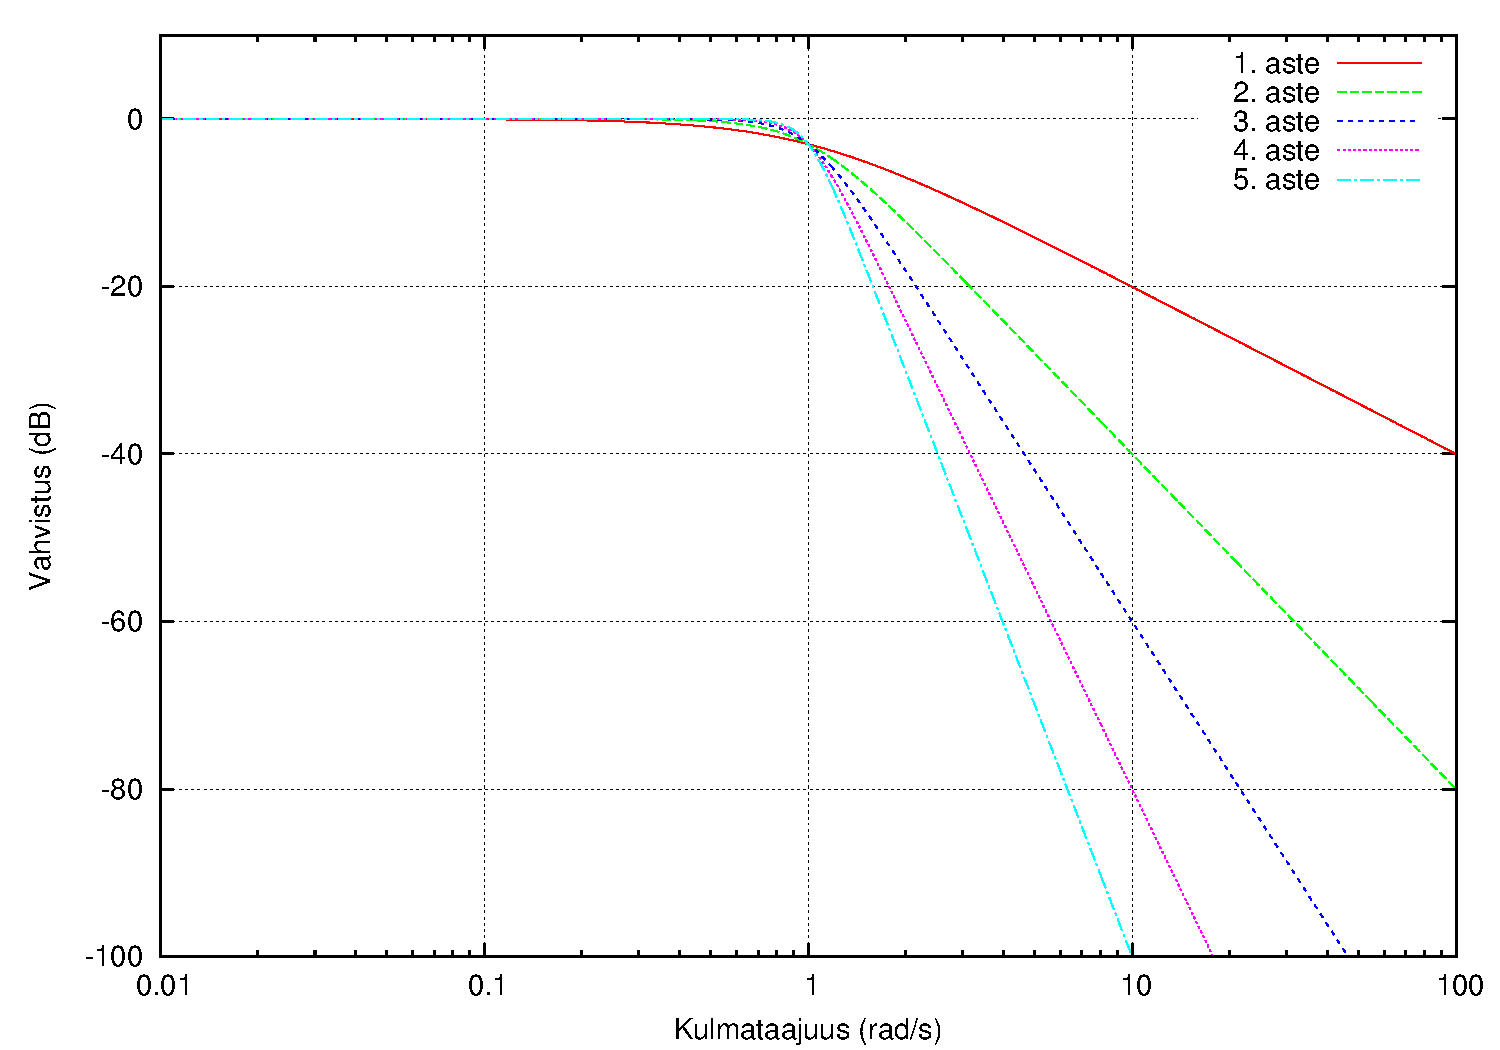
\includegraphics[height=8cm]{suodattimet_pics/bw.pdf}
}

\frame{
\frametitle{D-arvon vaikutus amplitudivasteeseen}
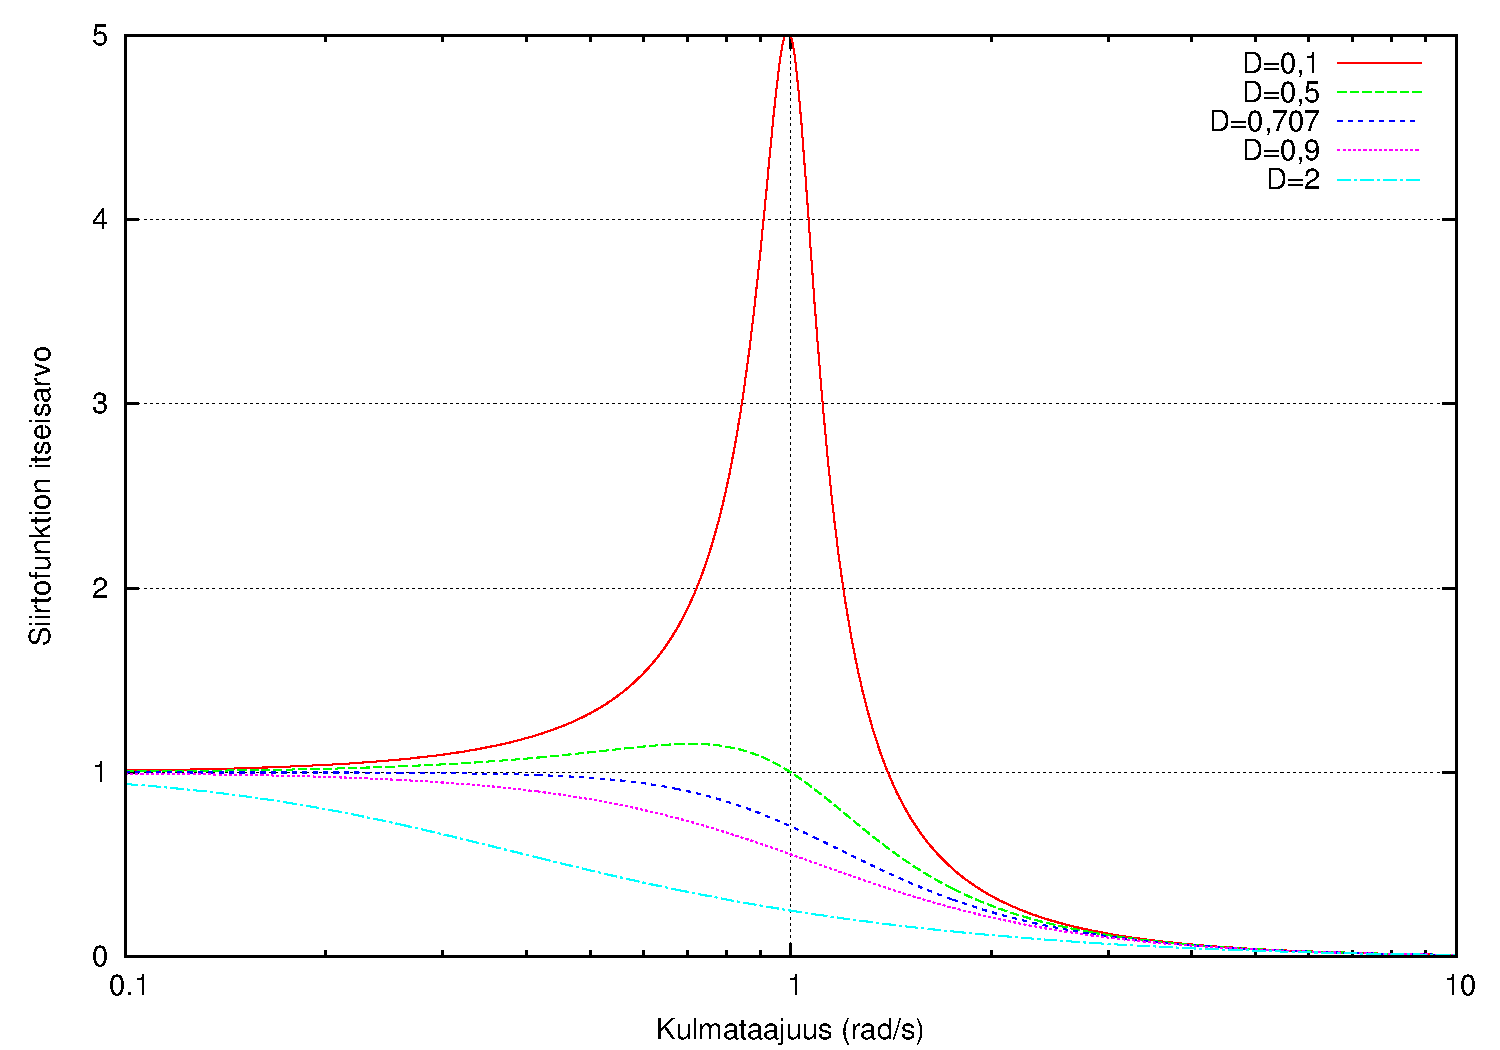
\includegraphics[height=8cm]{suodattimet_pics/d_arvo.pdf}
}

\frame{
\frametitle{Sallen-Key -alipäästösuodatin} \label{sallenkey}
\begin{center}

\begin{picture}(170,120)(0,0)

\du{0,0}{\Uin}
\hz{0,50}{R_2}
\hz{50,50}{R_1}
\vc{100,0}{C_1}
\hc{50,70}{}
\txt{75,90}{C_2}
\vo{100,50}{}{15}
\hg{100,0}
\hg{0,0}

\vln{50,50}{20}
\hln{100,100}{50}

\vln{100,70}{30}
\vln{150,60}{40}

\hln{150,60}{10}
\du{160,10}{\Uout}
\hg{160,10}

\end{picture}
\end{center}
\[
F(\jj\omega)=\frac{\Uout}{\Uin}=\frac{1}{(\jj\omega)^2C_1C_2R_1R_2+\jj\omega C_1(R_1+R_2)+1}
\]
}


\frame{
\frametitle{1. asteen ylipäästösuodatin}

\begin{itemize}
\item Siirtofunktio $\frac{s}{s+1} \to \frac{\frac{s}{\omega_0}}{\frac{s}{\omega_0}+1}$
\item Voidaan toteuttaa RC-piirillä
\end{itemize}

\begin{picture}(50,50)(-120,0)

\hc{0,50}{C}
\vz{50,0}{R}
\du{0,0}{\Uin}
\du{65,0}{\Uout}
\hln{0,0}{50}

\end{picture}

}

\frame{
\frametitle{2. asteen ylipäästösuodatin}
\begin{itemize}
\item Yleinen muoto $\frac{s^2}{s^2+2Ds+1} \to \frac{(\frac{s}{\omega_0})^2}{(\frac{s}{\omega_0})^2+2D\frac{s}{\omega_0}+1}$
\item Voidaan toteuttaa esim. Sallen-Key -piirillä
\item {\bf Tärkeää!} Ominaiskulmataajuudella ei välttämättä $|F(s)|=\frac{1}{\sqrt{2}}$
\end{itemize}
}


\frame{
\frametitle{Mitoitus ja taajuusmuunnokset}
\begin{itemize}
\item Haluttu piste ominaiskäyrällä voidaan siirtää muualle sijoittamalla $s\to s\frac{f_{\rm vanha}}{f_{\rm uusi}}$
\item Esimerkiksi jos siirtofunktion puolen tehon piste sijaitsee paikassa $\omega=42$ ja se halutaan taajuudelle
$f=500\Hz$, sijoitetaan siirtofunktioon jokaisen $s$:n paikalle $s\frac{42}{2\pi\cdot 500}$
\item Osoittajan kertominen vakiokertoimella ei vaikuta amplitudivasteen muotoon eikä vaiheeseen.
\item Mitoittamisen lähtökohtana on nimittäjäpolynomi, joka katsotaan taulukkokirjasta. Esim:
\begin{itemize}
\item Butterworth
\item Bessel
\item Legendre
\item \ldots
\end{itemize}
\end{itemize}
}




\frame{
\frametitle{Näin mitoitan suodattimen}
Esimerkki: Suunnittele toisen asteen Butterworth-alipäästösuodatin, jonka puolen tehon piste
on taajuudella 500 Hz. Toisen asteen Butterworth-polynomi on $(s^2+\sqrt{2}s+1)$.\\

Ratkaisun kulku:
\begin{enumerate}
\item Selvitetään, millä taajuudella sijaitsee puolen tehon piste alkuperäisellä siirtofunktiolla
\item Siirretään piste taajuudelle 500 Hz
\item Ratkaistaan $D$ ja $\omega_0$
\item (Rakennetaan piiri)
\end{enumerate}
}

\frame{
\frametitle{Selvitetään puolen tehon piste ja siirretään se}
Tasajännitteellä ($\omega=0$) vahvistus on 1, joten puolen tehon kulmataajuus on
\[
\Bigg|\frac{1}{s^2+\sqrt{2}s+1}\Bigg|=\frac{1}{\sqrt{2}}, s=\jj\omega_{1/2},
\]
josta ratkeaa $\omega_{1/2}=1$. Tämä piste saadaan siirrettyä taajuudelle 500 Hz tekemällä sijoitus
\[
s\to s\frac{1}{2\pi\cdot 500},
\]
jolloin siirtofunktioksi saadaan
\[
\frac{1}{(\frac{s}{2\pi\cdot 500})^2+\sqrt{2}\frac{s}{2\pi\cdot 500}+1}.
\]
}

\frame{
\frametitle{Ratkaistaan $\omega_0$ ja $D$}
Vertaamalla saatua siirtofunktiota yleiseen muotoon
\[
\frac{1}{(\frac{s}{2\pi\cdot 500})^2+\sqrt{2}\frac{s}{2\pi\cdot 500}+1}=\frac{1}{(\frac{s}{\omega_0})^2+2D\frac{s}{\omega_0}+1}
\]
nähdään, että $\omega_0=2\pi\cdot 500\approx 3140$ ja $D=\frac{1}{\sqrt{2}}$.
}

 \frame{
 \frametitle{Esimerkki}
\begin{center}
\begin{picture}(170,110)(0,0)

\du{0,0}{\Uin}
\hc{0,50}{C_2}
\hc{50,50}{C_1}
\vz{100,0}{R_1\hspace{-1mm}}
\hz{50,70}{}
\txt{75,90}{R_2}
\vo{100,50}{}{15}
\hg{100,0}
\hg{0,0}

\vln{50,50}{20}
\hln{100,100}{50}

\vln{100,70}{30}
\vln{150,60}{40}

\hln{150,60}{10}
\du{160,10}{\Uout}
\hg{160,10}

\end{picture}

\end{center}

Osoita, että kuvan piirin siirtofunktio on 2. asteen ylipäästöfunktio eli muotoa
\[
F(s)=\frac{\Uout}{\Uin}=\frac{(\frac{s}{\omega_0})^2}{(\frac{s}{\omega_0})^2+2D\frac{s}{\omega_0}+1}
\]
ja laske arvot $D$ ja $\omega_0$ (komponenttiarvojen funktiona). 


\tiny $\omega_0=\frac{1}{\sqrt{C_1C_2R_1R_2}}$ ja $D=\frac{1}{2}\frac{R_2(C_1+C_2)}{\sqrt{C_1C_2R_1R_2}}$} % TODO Kato missä määrin päällekkäinen resonanssi-suodattimet

\frame {
\frametitle{Yleismittari}
\begin{itemize}
\item Digitaalisen yleismittarin (DMM, digital multimeter) toiminta: jännite-, virta-, ja resistanssimittaus.
\item DMM perustuu jännitemittariin: virta mitataan mittaamalla vastuksen yli muodostuva jännite. Resistanssi mitataan mittaamalla vakiovirtalähteen resistanssiin syöttämän virran aiheuttama jännite
\item DMM on kelluva mittalaite, sen voi kytkeä "mihin tahansa".
\end{itemize}
 }


\frame {
\frametitle{Analoginen oskilloskooppi}
\begin{itemize}
\item Kuvan säädöt
\item Liipaisutoiminnot
\item Kahden jännitteen mittaaminen
\end{itemize}
\begin{alertblock}{Jos pitäisi valita yksi asia, mitä tältä kurssilta jokainen varmasti muistaisi, se olisi tämä!}
Oskilloskooppi {\bf ei ole} kelluva mittalaite: mittapään maadoitusklipsi on yhteydessä laitteen rungon kautta sähköverkon maahan. Mittapään maaklipsiä ei saa koskaan kytkeä mihinkään muualle kuin maahan!
\end{alertblock}
Joissain oskilloskoopeissa (esimerkiksi kannettavissa akkukäyttöisissä) tulot ovat kelluvia, mutta tämä on poikkeus ja siitä on maininta käyttöohjeessa.
 }


\frame {
\frametitle{Oskilloskoopin xy-asennon käyttö}
% TODO % Vois tehdä kalvon siitä XY-moden käytöstä, ks. TKK:n mittiksen labrapruju.

\begin{itemize}
\item Vaihe-eron mittaaminen xy-asennon avulla.

\end{itemize}
 }



\frame {
\frametitle{Mittaustekniikan terminologiaa}
\begin{itemize}
\item Mittaustekniikan termistö on standardoitu hyvin.
\end{itemize}
 }

\frame {
\frametitle{Mittausvirhe}
\begin{itemize}
\item Mittausvirhe = mittaustuloksen ja mitattavan arvon erotus. Mittausvirhe koostuu systemaattisesta ja satunnaisesta virheestä.
\item Systemaattinen virhe pysyy samana mittausta toistettaessa tai muuttuu jonkun säännön mukaan.
\item Systemaattista virhettä kutsutaan myös termillä {\em harha}.
\item Satunnainen virhe noudattaa usein normaalijakaumaa. 
\item Mittausepävarmuus sisältää sekä systemaattiset että satunnaiset virheet.
\end{itemize}
 }

\frame {
\frametitle{Tarkkuus}
\begin{itemize}
\item Usein puhekielessä sanotaan, että "mittalaitteen tarkkuus on 1 \%". Jos viilataan pilkkua, niin oikeampaa olisi puhua laitteen 1 \% epätarkkuudesta.
\item Tarkkuus on kvalitatiivinen termi.
\end{itemize}
 }

\frame {
\frametitle{Stabiilius}
\begin{itemize}
\item Mittalaitteen ominaisuudet muuttuvat, kun laite vanhenee.
\item Ominaisuudet muuttuvat myös, kun laite lämpenee. Juuri päälle kytketty mittalaite voi näyttää eri arvoa kuin kaksi tuntia päällä ollut.
\end{itemize}
 }

\frame {
\frametitle{Erottelukyky ja mittausalueen rajat}
\begin{itemize}
\item Erottelukyky tarkoittaa mittalaitteen kykyä reagoida mitattavan suureen pieniin muutoksiin. Esimerkiksi tavallisen yleismittarin erottelukyky herkimmällä
jännitemittausalueella on 0,1 millivolttia.
\item Valmistaja ilmoittaa myös mittausalueen ala- ja ylärajan. Esimerkiksi lämpömittarille: -50 --- +300$\, ^\circ \rm C$
\end{itemize}
 }

\frame {
\frametitle{Muita termejä}
\begin{description}
\item[Transparenssi] Mittalaitteen kyky olla muuttamatta mittaussuuretta.
\item [Vasteaika] Aikaväli siitä hetkestä, kun herätteessä esiintyy spesifioitu
äkillinen muutos, siihen hetkeen, kun vaste saavuttaa ja
jää spesifioitujen rajojen väliin, joiden sisällä on sen lopullinen
vakaa arvo.
\item [Kalibrointi] Toimenpiteet, joiden avulla spesifioiduissa olosuhteissa
saadaan mittauslaitteen tai mittausjärjestelmän näyttämien
tai kiintomitan tai vertailuaineen edustamien suureen
arvojen ja vastaavien mittanormaaleilla toteutettujen arvojen
välinen yhteys
\end{description}
 }

\frame {
\frametitle{Harjoitustehtävä}
\begin{itemize}
\item Kuinka suuri on oskilloskoopin tuloresistanssi?
\item Kuinka suuri on oskilloskoopin AC-tilan -3dB alarajataajuus?
\item Kuinka suuri on oskilloskoopin tulossa olevan AC-kytkentäkondensaattorin kapasitanssi?
\end{itemize}
Mitä mittauksia sinun on suoritettava? Tee mittaukset mahdollisimman tarkasti. Tee myös virhearvio!
 }




\frame {
\frametitle{Toistokoe}
\begin{itemize}
\item Mittaustuloksia käsitellään satunnaismuuttujina, joille voidaan laskea tunnuslukuja.
\item Tarkat tunnusluvut mittaustulosten jakaumalle saisi vain toistamalla mittausta äärettömän monta kertaa.
\item Kun havaintojen määrä on rajallinen, ovat otoksesta lasketut tunnusluvut todellisten tunnuslukujen estimaatteja.
\end{itemize}
 }

\frame {
\frametitle{Keskiarvo ja keskihajonta}
\begin{itemize}
\item Jakauman keskiarvon estimaatti on otoskeskiarvo
\[
\bar{x}=\frac{1}{N}\sum_{i=1}^N x_i,
\]
missä $N$ on havaintojen määrä.
\item Jakauman leveyttä kuvaa keskihajonta $\sigma$, jonka estimaatti on otoskeskihajonta
\[
s=\sqrt{\frac{\sum(x_i-\bar{x})^2}{N-1}}
\]

\item Otoskeskihajonta kuvaa hajontaa, jonka sisälle mahtuu 68 \% havainnoista. Kahden otoskeskihajonnan sisälle mahtuu 95 \% havainnoista. Tämä pätee, jos muuttuja oletetaan normaalijakautuneeksi!

\end{itemize}
 }

\frame {
\frametitle{Keskiarvon keskivirhe}
\begin{itemize}
\item Otoskeskihajonta kertoo alueen, jolle seuraavan mittaustuloksen pitäisi osua tietyllä todennäköisyydellä.
\item Laboratoriotutkimuksessa tehdään usein mittaussarja, josta lasketaan keskiarvo ja keskiarvolle jokin virheraja.
\item Virhearvio tälle keskiarvolle on keskiarvon keskivirhe
\[
\Delta \bar{x}=\frac{s}{\sqrt{N}}
\]
\item Keskiarvon keskivirhe kertoo, mille alueelle seuraavan mittaus{\bf sarjan} keskiarvo 68 \% todennäköisyydellä osuu, siinä missä otoskeskihajonta
kuvasi aluetta, jolle seuraava yksittäinen mittaus todennäköisesti osuu.
\end{itemize}
 }

\frame {
\frametitle{Virheen arviointi kokonaisdifferentiaalin avulla}
\begin{itemize}
\item Jos fysikaalista ilmiötä kuvaava matemaattinen malli tunnetaan, voidaan virheelle laskea yläraja-arvio derivoimalla funktio jokaisen muuttujan suhteen ja kertomalla osittaisderivaattojen itseisarvot muuttujien virhearvioilla:
\[
\Delta F=\left|\frac{\delta F}{\delta x_1}\right|\Delta x_1+\left|\frac{\delta F}{\delta x_2}\right|\Delta x_2+\ldots
\]
\item Itseisarvomerkkejä tarvitaan, koska virheelle haetaan yläraja-arviota, eikä haluta, että vastakkaismerkkiset virheet kumoavat toisiaan.
\end{itemize}
 }

\frame {
\frametitle{Lopputuloksen graafinen tarkastelu}
\begin{itemize}
\item Usein fysikaalista ilmiötä ei tutkita puhtaalla toistokokeella, vaan tehdään useita eri mittauksia ja tarkastellaan tuloksia graafisesti.
\item Graafisen tarkastelun avulla on helppo huomata lipsahdukset mittaustuloksissa sekä mallin pätemisen rajat. Lisäksi graafinen esitys on havainnollinen.

\end{itemize}
 }



\frame{
\frametitle{Mitä tässä on pielessä?}
\begin{columns}
\column{5cm}
Mitataan jännitteen ja virran arvot, lasketaan joka riviltä resistanssi Ohmin lailla

\begin{tabular}{ l  l | l}
$U$(V) & $I$(A) & $R$($\Omega$)\\
1,32 & 0,50 & 2,64\\
2,37 & 1,00 & 2,37\\
3,15 & 1,50 & 2,10\\
4,23 & 2,00 & 2,12\\
5,40 & 2,50 & 2,16\\
6,20 & 3,00 & 2,07\\
\end{tabular}

ja lasketaan resistanssien keskiarvo, joka on 2,24 ohmia ja keskiarvon keskivirhe 0,09, ja päätellään, että resistanssi on
\[
R=(2,24 \pm 0,09)\, \Omega.
\]

\column{40mm}
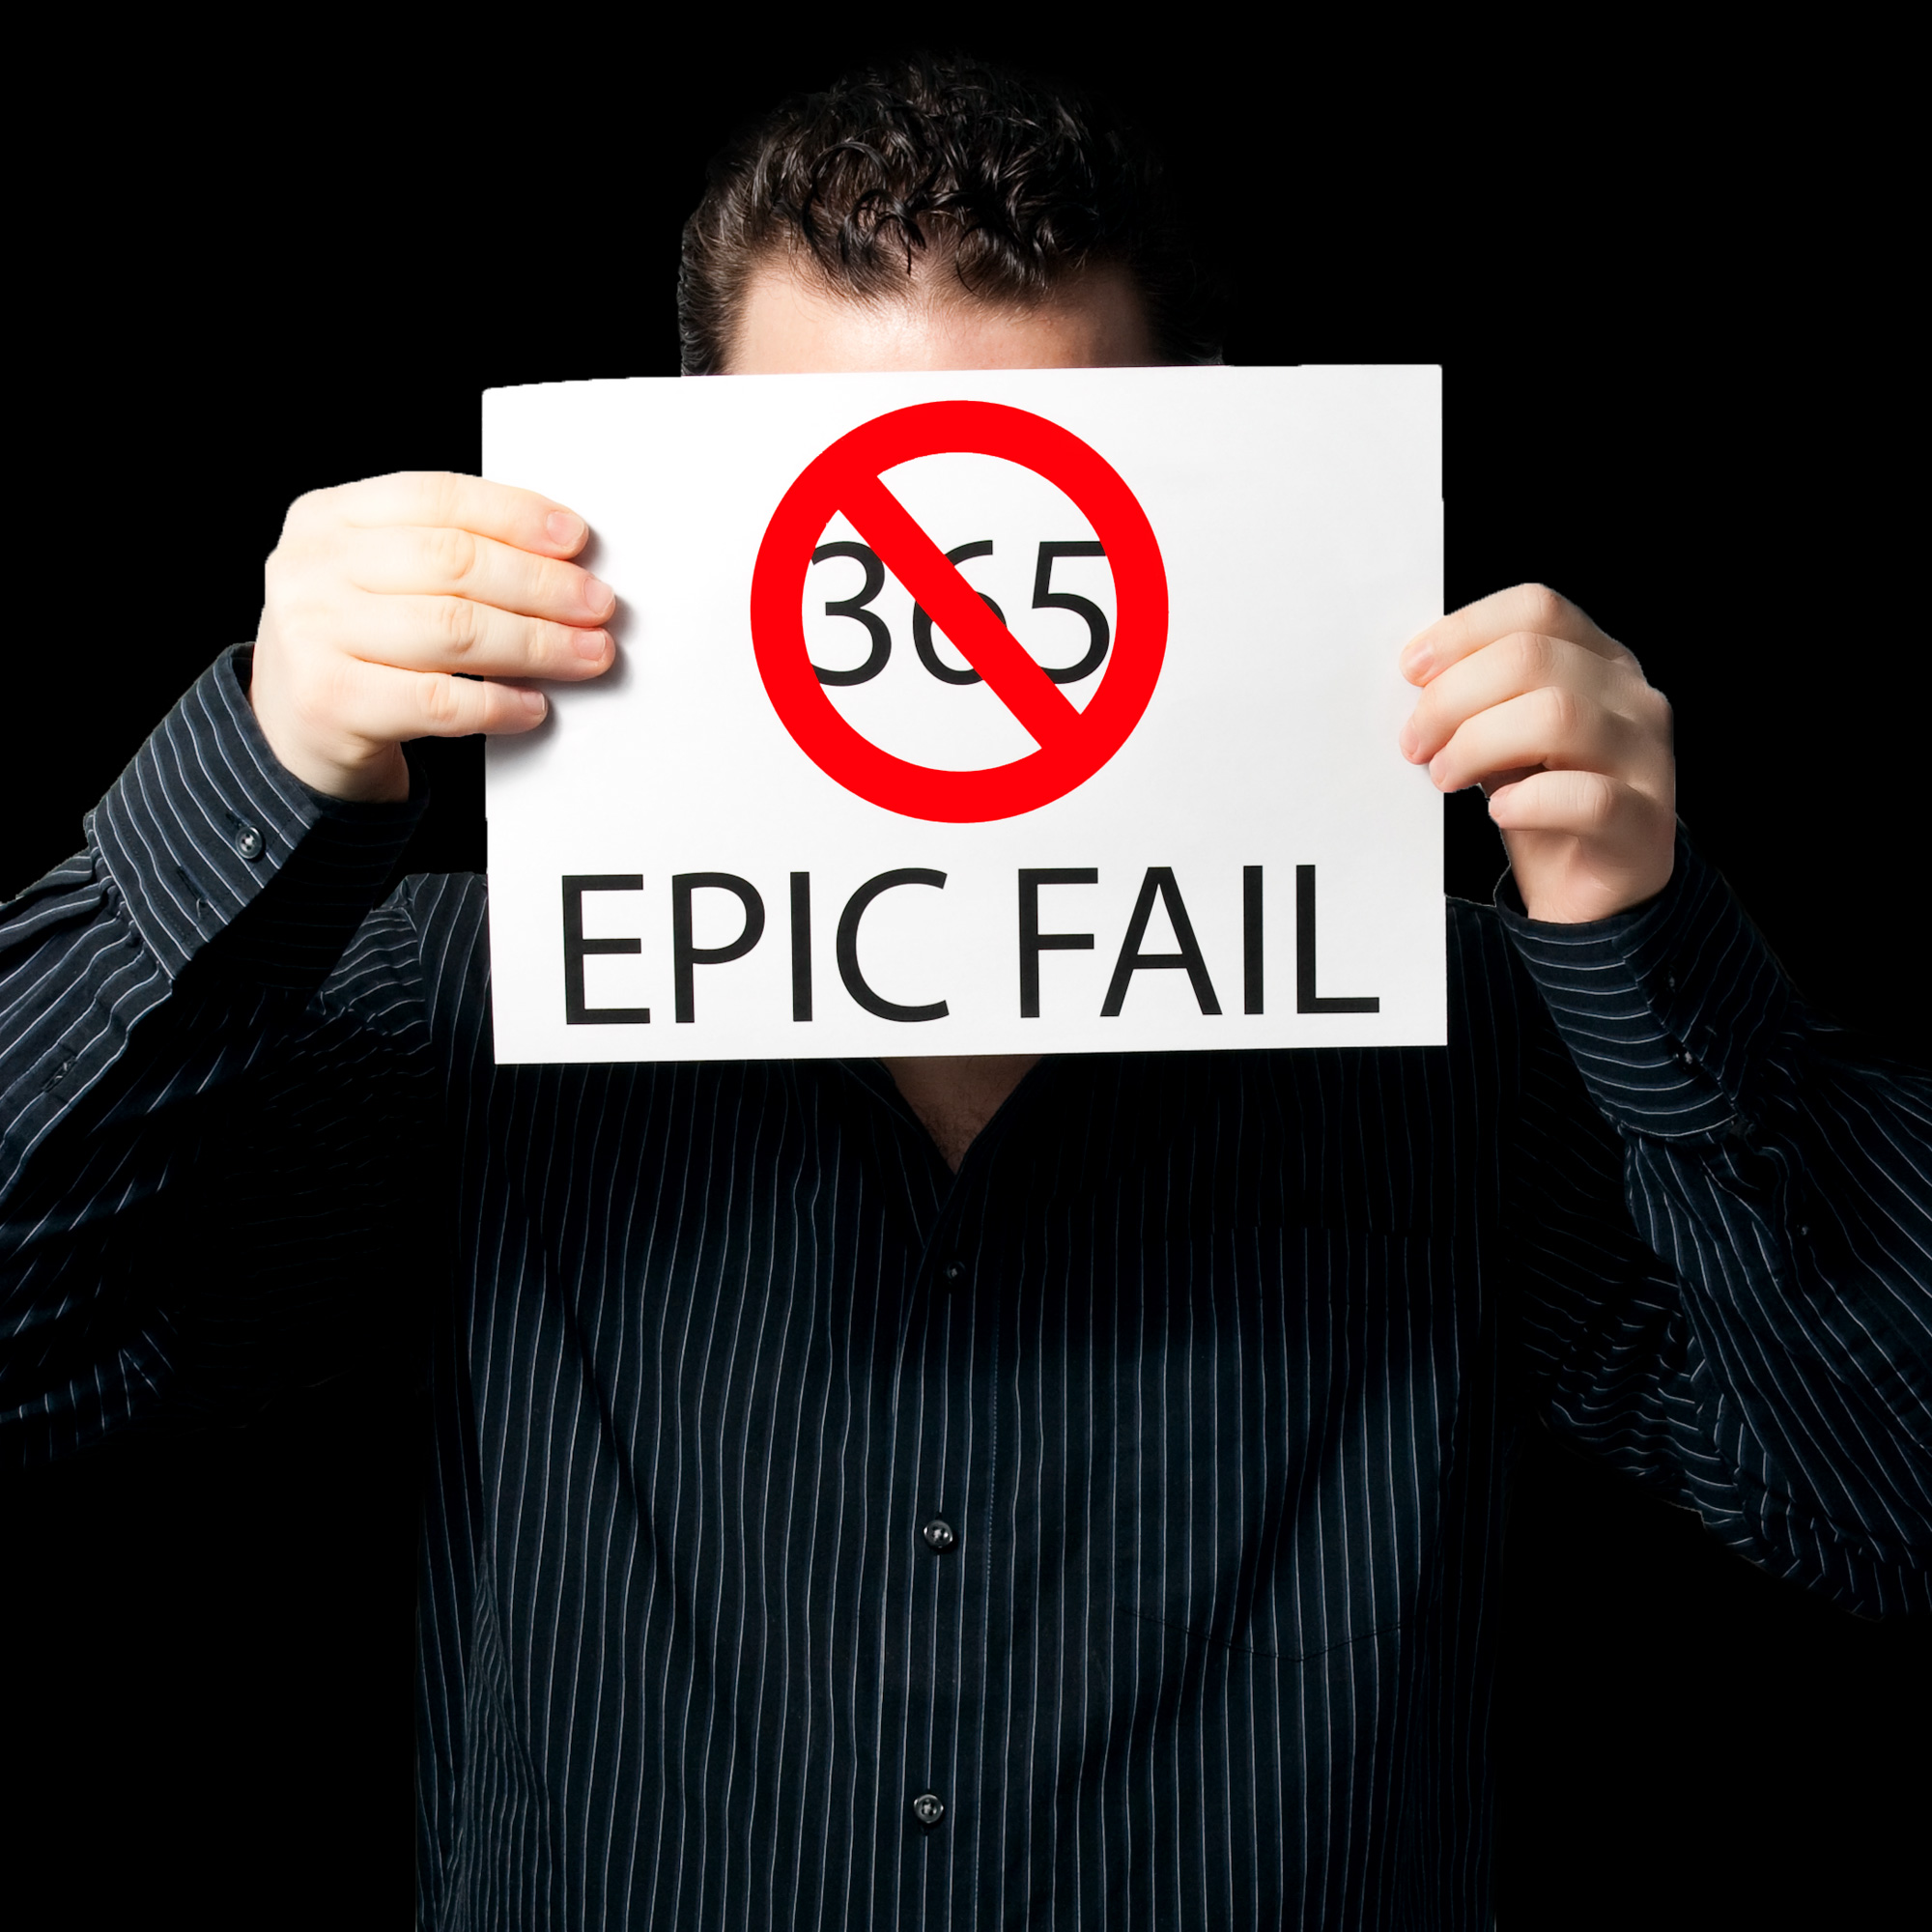
\includegraphics[width=40mm]{mittaustekniikka_pics/epicfail.jpg}

\tiny{\url{http://www.flickr.com/photos/28091490@N03/4277085203/}}

\vfill

\end{columns}

}

\frame {
\frametitle{Mitä on pielessä?}
\begin{itemize}
\item Mittaus {\bf ei ole toistokoe}. Mitattavat suureet muuttuvat.
\item Menetelmä on herkkä systemaattiselle virheelle (esimerkiksi jos mittari näyttää jatkuvasti liikaa).
\item Ohmin lain pätevyyttä ei testata, vaan se oletetaan päteväksi.
\item {Mittaustarkkuutta ei oteta huomioon ollenkaan!}
\end{itemize}
 }

\frame {
\frametitle{Oikea tapa}
\begin{itemize}
\item Selvitetään mittalaitteiden virheet (tässä esimerkissä olkoot 0,4 V ja 0,01 A).
\item Merkitään mittapisteet millimetripaperille\footnote{Esimerkiksi \url{http://www.csun.edu/science/ref/measurement/data/graphpaper/mm.pdf}}.
\item Pyri käyttämään koko millimetripaperi hyväksesi eli valitse asteikot järkevästi.
\item Piirretään mahdollisimman hyvin pisteiden kautta kulkeva suora.
\item Piirretään virhesuorat eli rajat sille, kuinka loiva tai jyrkkä suora voi pahimmillaan olla.
\item Lasketaan resistanssi suoran kulmakertoimesta.
\item Lasketaan virhearvio resistanssille virhesuorien kulmakertoimien keskiarvona.
\end{itemize}
 }

\frame {
\frametitle{Kirjallisuutta}
\begin{itemize}
\item Standardi SFS 3700\footnote{Standardi on kumottu ja korvattu käsikirjalla SFS-OPAS 99. Ei olennaisia muutoksia.}: Metrologia. Perus- ja yleistermien sanasto.
\item Pekka Wallin: Sähkömittaustekniikan perusteet. 6. painos. Helsinki 2001.
\item Pietiläinen, Merimaa: Mittaustekniikan perusteiden laboratoriotyöt. 7. korjattu painos. Helsinki 2000.
\item Kalle Ojanen: Virhelaskennan alkeita. \url{http://www.physics.utu.fi/opiskelu/opiskelijaksi/tyokurssi/index/Virhelaskkokonaan.pdf} Viitattu 31.3.2011.
\item TKK: Mittaustulosten käsittely: \url{http://tfy.tkk.fi/kurssit/Tfy-3.15x/Teoria/Tulostenkasittely.pdf} Viitattu 31.3.2011.
\end{itemize}
 }


\frame{
\frametitle{Sinimuotoinen vaihtojännite}
\begin{itemize}
\item Pistorasiasta saatava jännite on {\em sinimuotoista}.
\item Kaikki jaksolliset vaihtojännitteet voidaan esittää siniaaltojen summana
(Fourier'n teoreema).
\item Lineaarisessa piirissä sinimuotoinen heräte tuottaa sinimuotoisen vasteen.
\item Sinimuotoisilla signaaleilla laskeminen on helppoa.
\end{itemize}
}



\frame{
\frametitle{Sinimuotoinen jännite (tai virta)}
Sinimuotoinen jännite (tai virta) määritellään
\[
u(t)=\hat{u}\sin(2\pi f t+ \phi)
\]
Usein merkitään $\omega=2\pi f$, jolloin kaava lyhenee:
\[
u(t)=\hat{u}\sin(\omega t+ \phi)
\]
Suuretta $\omega$ kutsutaan {\em kulmataajuudeksi} ja sen yksikkö on $\frac{\rm rad}{\rm s}$. Kulma $\phi$ on {\em vaihekulma}.
Kerroin $\hat{u}$ (luetaan u-hattu) on jännitteen {\em amplitudi} eli huippuarvo. Huippuarvosta saadaan jännitteen {\em tehollisarvo} jakamalla
se luvulla $\sqrt{2}$.
}

\frame{
\frametitle{Kondensaattori ja sinimuotoinen jännite}
Yhtälöstä
\[
i=C\Du
\]

\begin{center}
\begin{picture}(50,50)(0,0)
\vst{-25,0}{u(t)=\hat{u}\sin(\omega t+ \phi)}
\vc{25,0}{C}
\di{25,40}{i}
%\du{40,0}{u}
\hln{-25,0}{50}
\hln{-25,50}{50}

\end{picture}
\end{center}
Virta on siis
\[
i=C\Du=C\omega\hat{u}\cos(\omega t+ \phi)=C\omega\hat{u}\sin(\omega t+ \phi+\frac{\pi}{2})
\]
Eli jännitteen ja virran suhde on $\frac{1}{C\omega}$, ja niiden välillä on 90 asteen ($\frac{\pi}{2}$
radiaanin) vaihe-ero. Virta on 90 astetta jännitettä edellä.
}

\frame{
\frametitle{Reaktanssin käsite}
Kondensaattorille
\[
i=C\Du
\]

\begin{center}
\begin{picture}(50,50)(0,0)
\vst{-25,0}{u(t)=\hat{u}\sin(\omega t+ \phi)}
\vc{25,0}{C}
\di{25,40}{i}
%\du{40,0}{u}
\hln{-25,0}{50}
\hln{-25,50}{50}

\end{picture}
\end{center}
\[
i(t)=C\Du=C\omega\hat{u}\cos(\omega t+ \phi)=C\omega\hat{u}\sin(\omega t+ \phi+\frac{\pi}{2})
\]
Jännitteen ja virran {\bf amplitudien} suhde on:
\[
X=\frac{\hat{u}}{C\omega \hat{u}}=\frac{1}{\omega C}
\]
Tätä jännitteen ja virran suhdetta $X$ kutsutaan {\bf reaktanssiksi}, aivan kuten jännitteen ja virran suhdetta
vastuksessa kutsutaan resistanssiksi.
}

\frame{
\frametitle{Kela ja sinimuotoinen jännite}
Yhtälöstä
\[
u=L\Di
\]

\begin{center}
\begin{picture}(50,50)(0,0)
\vj{-25,0}{i(t)=\hat{i}\sin(\omega t+ \phi)}
\vl{25,0}{L}
\di{25,40}{i}
\du{40,0}{u}
\hln{-25,0}{50}
\hln{-25,50}{50}

\end{picture}
\end{center}
Jännite on 
\[
u=L\Di=L\omega\hat{i}\cos(\omega t+ \phi)=L\omega\hat{i}\sin(\omega t+ \phi+\frac{\pi}{2})
\]
Eli jännitteen ja virran suhde on ${L\omega}$, ja niiden välillä on 90 asteen ($\frac{\pi}{2}$
radiaanin) vaihe-ero. Virta on 90 astetta jännitettä jäljessä.
}

\frame{
\frametitle{Kelan reaktanssi}
Yhtälöstä
\[
u=L\Di
\]

\begin{center}
\begin{picture}(50,50)(0,0)
\vj{-25,0}{i(t)=\hat{i}\sin(\omega t+ \phi)}
\vl{25,0}{L}
\di{25,40}{i}
\du{40,0}{u}
\hln{-25,0}{50}
\hln{-25,50}{50}

\end{picture}
\end{center}
Jännite on 
\[
u=L\Di=L\omega\hat{i}\cos(\omega t+ \phi)=L\omega\hat{i}\sin(\omega t+ \phi+\frac{\pi}{2})
\]
Jännitteen ja virran suhde eli kelan reaktanssi on:
\[
X=\frac{L\omega\hat{i}}{\hat{i}}=\omega L
\]
}

\frame{
\begin{block}{Esimerkki} % TODO: Ratkaisu puuttuu
Kuinka suuri on virran $I$ a) tehollisarvo b) huippuarvo ($\hat{i}$). Onko virta jännitettä edellä vai jäljessä,
ja kuinka paljon? Jännitelähteen taajuus on 50 Hz ja tehollisarvo 230 volttia.
\end{block}
\begin{center}
\begin{center}
\begin{picture}(50,50)(0,0)
\vst{-25,0}{E}
\vc{25,0}{C}
\di{25,40}{I}
%\du{40,0}{u}
\hln{-25,0}{50}
\hln{-25,50}{50}

\end{picture}
\end{center}
\[
C=1\uF
\]
\end{center}

}


\frame{
\frametitle{Esimerkki} % Arska 1 kotitehtävä 1 2009
\[
J=1\A\ (f=50\Hz)\quad L=1\,{\rm H} \quad C=100\uF
\]

\begin{center}
\begin{picture}(150,110)(0,0)
\vj{0,0}{J}
\vc{50,0}{C}
\vl{50,50}{L}
\hln{0,0}{50}
\hln{0,100}{50}
\vln{0,50}{50}
\du{70,0}{u_{\rm C}}
\du{70,50}{u_{\rm L}}

\end{picture}
\end{center}
Laske jännitteet $u_{\rm C}$ ja $u_{\rm L}$ ja ilmoita ne ajan funktiona muodossa $u=\hat{u}\sin(\omega t+\phi)$. Miksi näiden jännitteiden tehollisarvojen (tai huippuarvojen) summa
ei ole suoraan virtalähteen jännite?

\tiny $u_{\rm L}\approx 444\V\cdot\sin(2\pi 50\Hz\cdot t+90^\circ)$, $u_{\rm C}\approx 45\V\cdot\sin(2\pi 50\Hz\cdot t-90^\circ)$
}


% TODO Korosta, että vastaus (virta tai jännite) aina kulmamuodossa! RI-muoto ei kerro mitään.
% TODO Mieti asioiden esittelyjärjestystä (kompleksiluvut vs. niiden soveltaminen).

\frame{
\frametitle{Kompleksiluvut}
\begin{itemize}
\item Vaihtosähköpiirilaskuja on helppo laskea osoittimilla.
\item Osoittimia on puolestaan helppo käsitellä kompleksilukujen avulla.
\end{itemize}
}

\frame{
\frametitle{Kompleksiluvut}
Kompleksilukuaritmetiikka perustuu imaginaariyksikköön i, joka määritellään seuraavasti:
\[
{\rm i}^2=-1
\]
Perinteisessä reaalilukuaritmetiikassa mikään luku korotettuna toiseen ei ole -1, mutta
mikään ei estä määrittelemästä sellaista. Ettei pikku-i mene sekaisin virran kanssa, sähkötekniikassa
imaginaariyksikölle käytetään symbolia $\jj$:
\[
\jj^2=-1
\]
}

\frame{
\frametitle{Kompleksiluvut}
Kompleksiluku jakaantuu reaaliosaan ja imaginaariosaan. Esimerkiksi jos lasketaan yhteen reaaliluku 3 ja 
imaginaariyksikkö $\jj$, saadaan luku
\[
3+\jj
\]
 }

\frame{
\frametitle{Laskeminen kompleksiluvuilla}
Peruslaskutoimitusten  laskeminen kompleksiluvuilla ei käytännössä eroa reaaliluvuilla laskemisesta:
\[
3(\jj + 2)= 3\jj + 6
\]
\[
(1+2\jj)(1+\jj)=1+\jj+2\jj + 2\jj^2=1+3\jj -2=-1+3\jj
\]



}

\frame{
\frametitle{Eulerin kaava}
Kompleksiluvuille pätee Eulerin kaava. Sen todistaminen on mahdollista sarjakehitelmien avulla
ja kuuluu (yliopisto)matematiikan tunnille. Otamme kaavan käyttöön perustelematta:
\[
e^{\jj \phi}=\cos \phi + \jj \sin \phi
\]
Eulerin kaava on tärkeä, kun kompleksilukuja muunnetaan summamuodosta kulmamuotoon.
Kompleksitason piste $2+2\jj$ voidaan esittää joko summamuodossa:
\[
z=2+2\jj
\] 
tai kulmamuodossa (Eulerin kaavan avulla)
\[
2\sqrt{2}\cdot e^{\jj\frac{\pi}{4}}=2\sqrt{2}\left(\cos \frac{\pi}{4} +\jj\sin\frac{\pi}{4} \right)
\]
Kompleksiluvun $2+2\jj$ kulma eli argumentti on $\frac{\pi}{4}$ radiaania eli 45 astetta ja itseisarvo on $2\sqrt{2}$.
}

\frame{
\frametitle{Eulerin kaavan geometrinen tulkinta}
Kompleksiluvun itseisarvo tarkoittaa kompleksitason pisteen etäisyyttä origosta. Kompleksiluvun
kulma tarkoittaa pisteen suuntaa $x$-akselilta katsottuna.

Eulerin kaavan käyttö ei ole itsetarkoitus sähkötekniikassa. Sen takia kulmamuodossa olevaa kompleksilukua
ei kirjoiteta näkyviin muodossa $r e^{\phi \jj}$, vaan käytetään muotoa $r\angle \phi$. Kyseessä on vain
lyhennysmerkintä.
}


\frame{
\frametitle{Kompleksiluku}
Kompleksiluku $z$ voidaan esittää joko reaali-imaginaarimuodossa
\[
z=x+y\jj
\]
tai kulmamuodossa
\[
z=r\angle \phi
\]
Muunnoskaavat ovat
\[
r=\sqrt{x^2+y^2} \quad {\rm ja} \quad \phi=\arctan\frac{y}{x}
\]
ja toiseen suuntaan
\[
x=r\cos \phi \quad {\rm ja} \quad y=r\sin \phi
\]
Kyse ei ole sen monimutkaisemmasta asiasta, kuin että pisteen sijainti koordinaatistossa, jossa x-akseli
kuvaa reaaliosaa ja y-akseli imaginaariosaa.
}

\frame{
\frametitle{Älä tee näin!}
\begin{columns}
\column{5cm}
Joka vuosi kokeessa joku korottaa imaginaariyksikön vahingossa toiseen,
kun laskee kompleksiluvun itseisarvoa:
$z=3 + 4\jj \Rightarrow r=\sqrt{3^2 + (4{\color{red}\jj})^2}$
$\color{red}=\sqrt{9-16}=\sqrt{-7}$

Oikein on:
$z=3 + 4\jj \Rightarrow r=\sqrt{3^2 + 4^2}$
$=\sqrt{9+16}=\sqrt{25}=5$.

Kyse ei ole mistään monimutkaisemmasta kuin Pythagoraan lauseen soveltamisesta,
sinne ei imaginaariyksikköä sotketa!

\column{40mm}
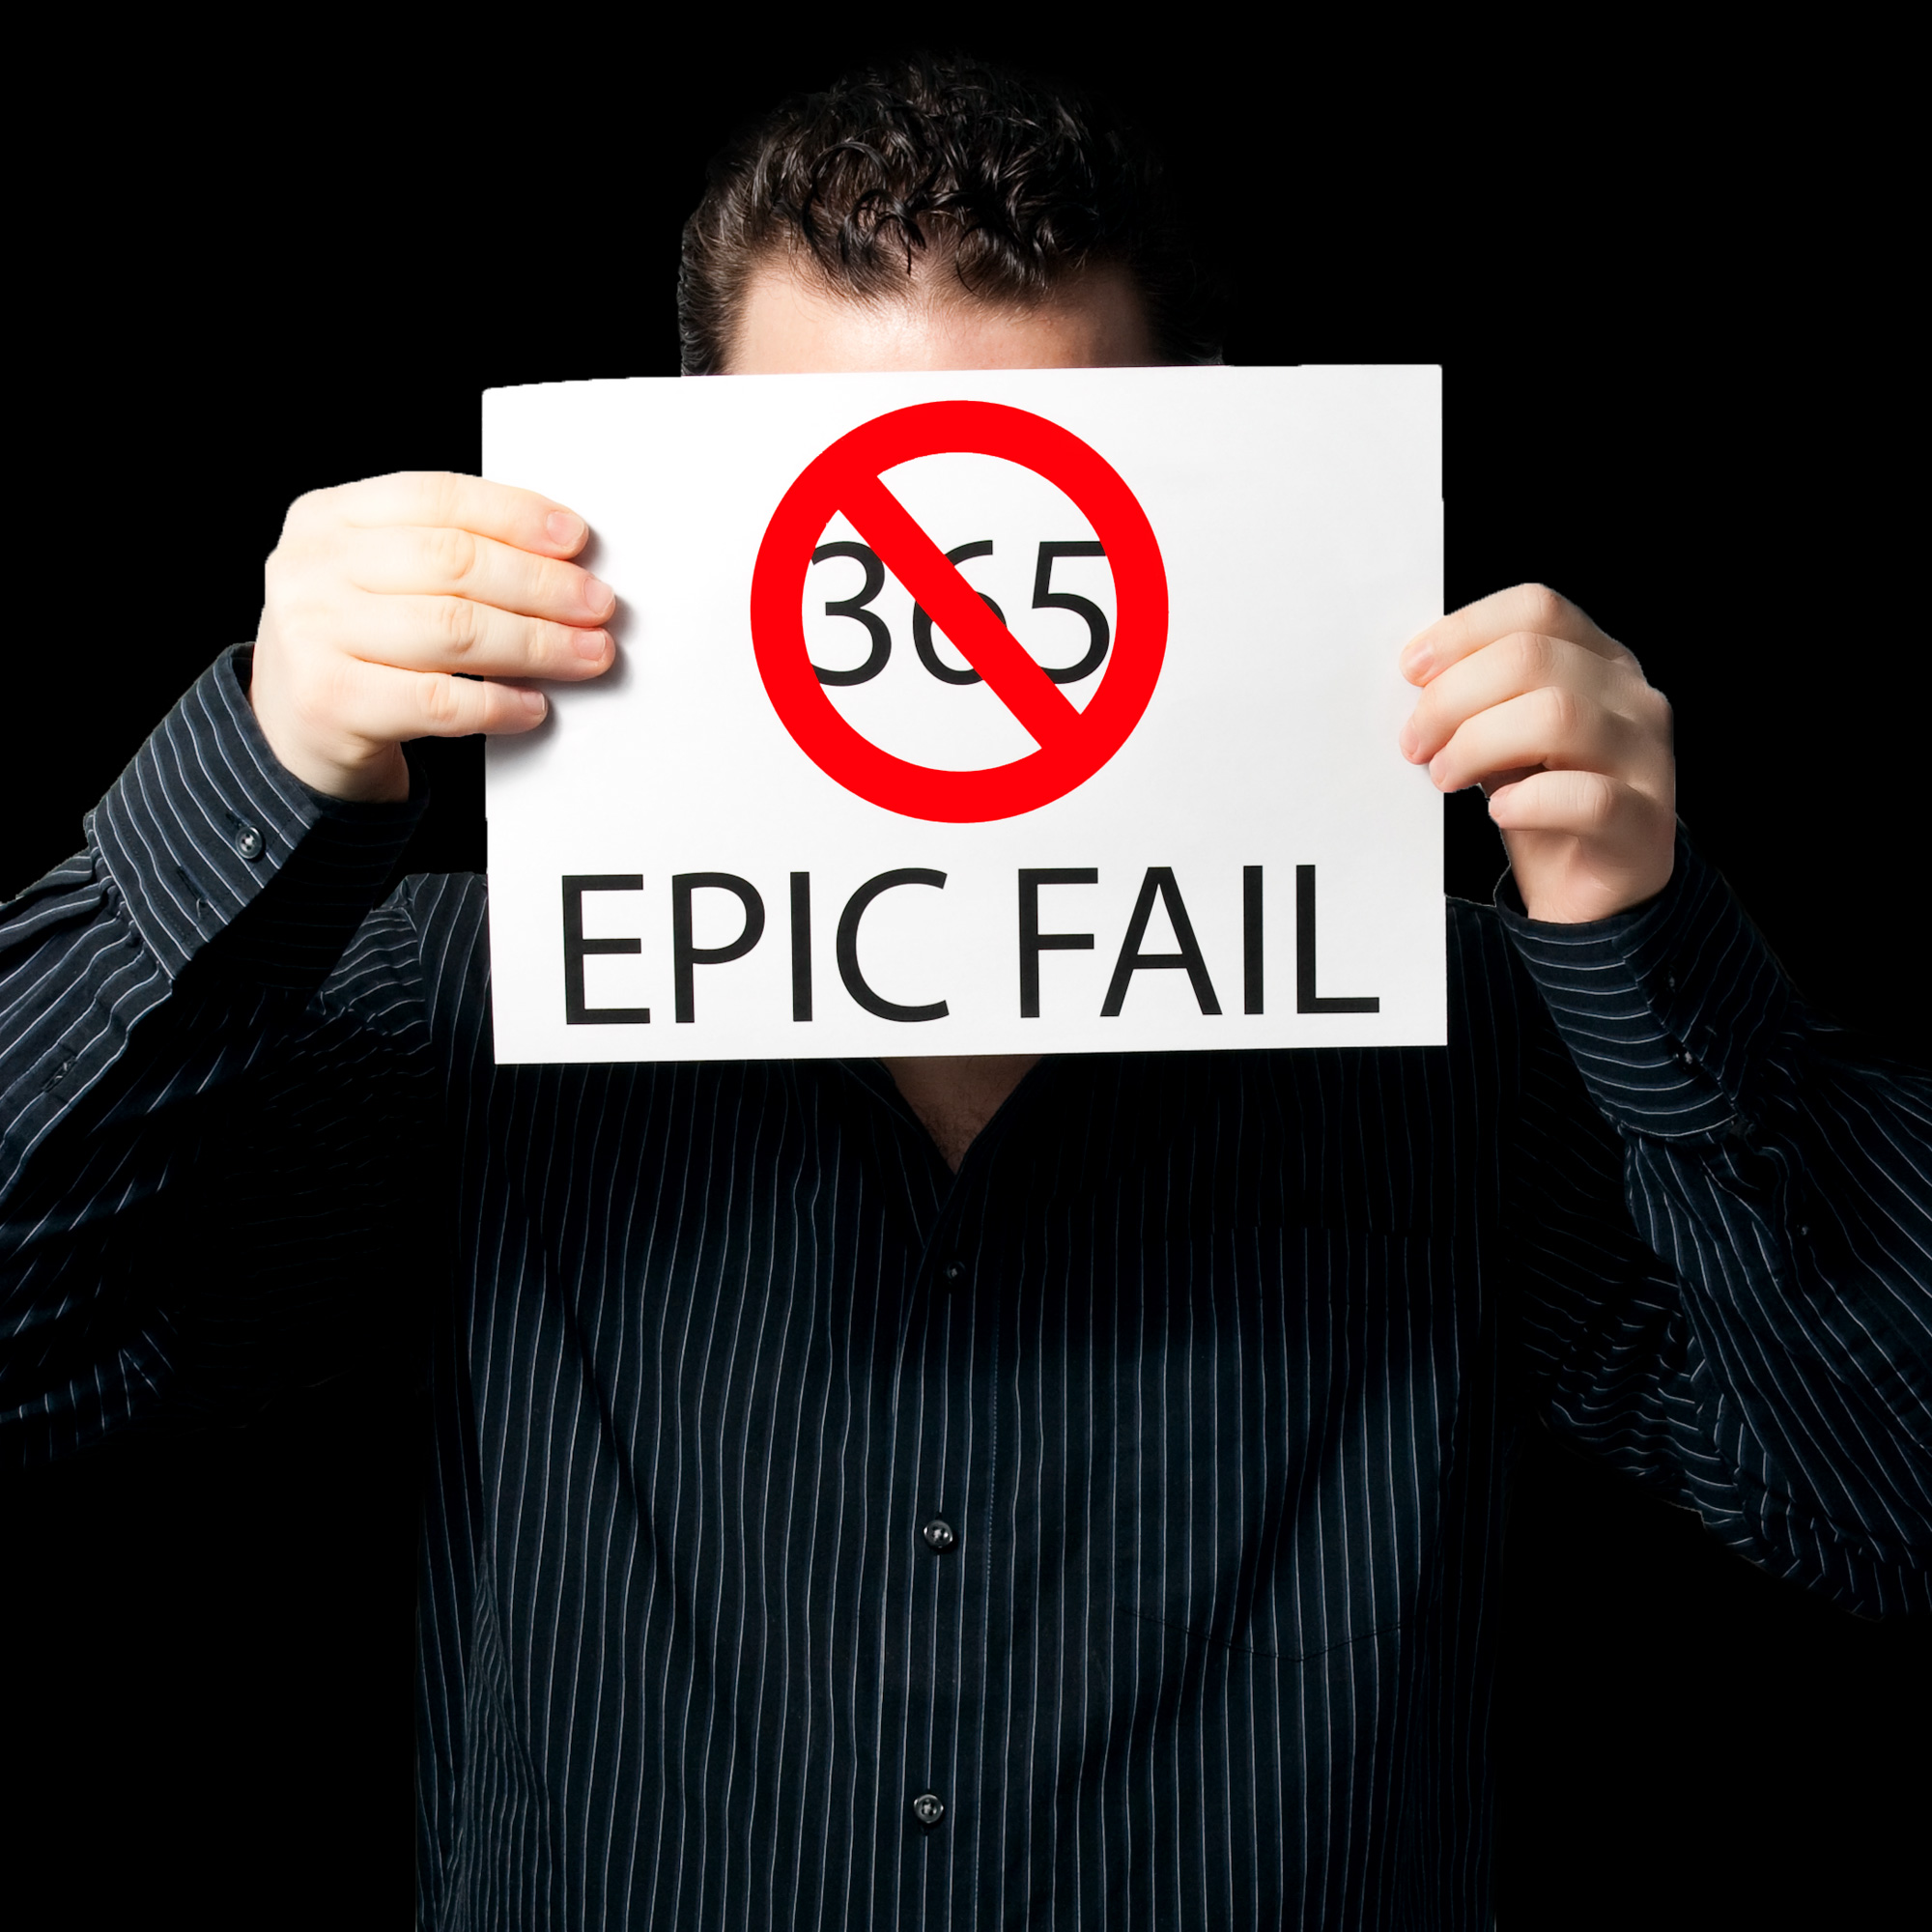
\includegraphics[width=40mm]{mittaustekniikka_pics/epicfail.jpg}
\end{columns}
}


\frame{
\frametitle{Kompleksilukujen laskusääntöjä}
Nyrkkisääntö: yhteen- ja vähennyslaskut ovat helppoja reaali-imaginaarimuodossa
($x+y\jj$), jako- ja kertolasku ovat helppoja kulmamuodossa.

Kertolasku kulmamuodossa:
\[
r_1\angle\phi_1 \cdot r_2\angle\phi_2=(r_1r_2)\angle \phi_1+\phi_2
\]
eli itseisarvot kerrotaan keskenään, ja kulmat lasketaan yhteen.

Jakolasku kulmamuodossa:
\[
\frac{r_1\angle\phi_1}{r_2\angle\phi_2}=\frac{r_1}{r_2}\angle \phi_1-\phi_2
\]
eli itseisarvoille suoritetaan jakolasku ja kulmat vähennetään toisistaan.
}





\frame{
\frametitle{Osoitinlaskenta kompleksiluvuilla (johdanto)}
\begin{itemize}
\item Jos piirissä on yksi lähde ja yksi kela tai kondensaattori, lasku on helppo.
\item Jos niitä on useampi, laskeminen on mielettömän työlästä.
\item Onneksi voidaan käyttää kompleksilukuihin perustuvaa {\bf osoitinlaskentaa}.
\item Osoitinlaskennassa jännitteet ja virrat ovat kompleksilukuja, jotka sisältävät
sekä jännitteen tehollisarvon että vaihekulman.
\end{itemize}

}

\frame{
\frametitle{Tehollisarvon käsite}
\begin{itemize}
\item Osoitinlaskennassa käytetään tehollisarvon osoittimia, koska tällöin 
tehon kaava on siistimmän muotoinen kuin huippuarvon osoittimia käytettäessä.
\item Vaihtosähköteho käsitellään seuraavalla tunnilla: nyt riittää, että tiedämme, että:
\item Sinimuotoisen vaihtovirran ja -jännitteen huippuarvon ja tehollisarvon suhde on $\sqrt{2}$.
\item Tehollisarvolla tarkoitetaan sitä, kuinka suurta tasajännitettä vaihtojännite vastaa
lämmitysteholtaan, jos siihen kytketään resistiivinen kuorma. Esimerkiksi hehkulamppu
loistaa yhtä kirkkaasti, kytkipä sen 230 voltin akustoon (tasajännite) tai 230 voltin verkkosähköön
(vaihtojännite). Verkkojännitteen huippuarvo on $230\cdot \sqrt{2}\approx325$ volttia.
\end{itemize}

}

\frame{
\frametitle{Osoitinlaskenta kompleksiluvuilla}
\begin{itemize}
\item Uusi käsite: impedanssi ($Z$). Vastuksen impedanssi on $R$. Kelan
impedanssi $Z_L=\jj \omega L$ ja kondensaattorin impedanssi $Z_C=\frac{1}{\jj \omega C}$. 
\item $\jj$ on matematiikan tunnilta tuttu imaginaariyksikkö: $\jj^2=-1$.
Sähkötekniikassa ei käytetä lyhennettä $i$, koska se tarkoittaa virtaa.
\item Jännite ja virta ilmaistaan kompleksilukuna siten, että kompleksiluvun
itseisarvona on jännitteen/virran tehollisarvo ja kulmana (argumenttina)
jännitteen/virran vaihekulma.
\item $u= \hat{u}\sin(\omega t+ \phi) \Leftrightarrow U=\frac{\hat{u}}{\sqrt{2}}\angle\phi$
\item Merkintä $r\angle \phi$ tarkoittaa kompleksilukua, jonka itseisarvo on $r$ ja argumentti
$\phi$.
\end{itemize}

}

\frame{
\frametitle{Kondensaattori ja sinimuotoinen jännite osoitinlaskennalla}
Aiempi esimerkki osoitinlaskennalla.

\begin{center}
\begin{picture}(50,50)(0,0)
\vst{-25,0}{u(t)=\hat{u}\sin(\omega t+ \phi)}
\vc{25,0}{C}
\di{25,40}{i}
%\du{40,0}{u}
\hln{-25,0}{50}
\hln{-25,50}{50}

\end{picture}
\end{center}
Muunnetaan jännitelähteen arvo kompleksiluvuksi:
$u(t)=\hat{u}\sin(\omega t+ \phi) \Rightarrow U=\frac{\hat{u}}{\sqrt{2}}\angle \phi$.
Virta on Ohmin lain mukaan
\[
I=\frac{U}{Z}=\frac{\frac{\hat{u}}{\sqrt{2}}\angle \phi}{\frac{1}{\jj\omega C}}=\jj\omega C\cdot \frac{\hat{u}}{\sqrt{2}}\angle \phi
=\omega C\angle90^\circ \cdot \frac{\hat{u}}{\sqrt{2}}\angle \phi=
\frac{\hat{u}\omega C}{\sqrt{2}}\angle \phi+90^\circ
\]
Muunnetaan takaisin ajan funktioksi:
\[
i=C\omega\hat{u}\sin(\omega t+ \phi+\frac{\pi}{2})
\]
Eli jännitteen ja virran suhde on $\frac{1}{C\omega}$ ja niiden välillä on 90 asteen ($\frac{\pi}{2}$
radiaanin) vaihe-ero. Virta on 90 astetta jännitettä edellä.
}

\frame{
\frametitle{Osoitinlaskennan teoreettinen perusta}
\scriptsize
\begin{itemize}
\item Jokainen sinimuotoinen jännite ja virta voidaan ajatella pyörivänä viisarina. Viisari pyörii
kulmanopeudella $\omega$ ja sen pituus on jännitteen/virran huippuarvo (jos lasketaan huippuarvoilla)
tai tehollisarvo (jos lasketaan tehollisarvoilla).
\item Vaihekulma $\phi$ kertoo kohdan, josta viisari lähtee pyörimään.
\item Jos kelaan syötetään virta $I$, kelan jännite on 90 astetta $I$:tä edellä ja jännitteen suuruus
on $\omega L$-kertainen.
\item Kelan jänniteviisari saadaan virtaviisarista siis kääntämällä viisaria 90 astetta eteenpäin ja
kasvattamalla sen pituus $\omega L$-kertaiseksi.
\item Jos kondensaattoriin syötetään virta $I$, kondensaattorin jännite on 90 astetta virtaa $I$ jäljessä
ja jännite on $\frac{1}{\omega C}$-kertainen.
\item Kondensaattorin jänniteviisari saadaan virtaviisarista siis kääntämällä viisaria 90 astetta taaksepäin ja
kasvattamalla sen pituus $\frac{1}{\omega C}$-kertaiseksi.
\item Kompleksilukujen laskusäännöt sopivat tähän kuin nyrkki silmään: kertomalla virta kompleksisella
impedanssilla, muuttuu sekä pituus että vaihe. $\jj$:llä kertominenhan kääntää kompleksiluvun kulmaa
eteenpäin ja $\jj$:llä jakaminen taaksepäin 90 astetta.
\item Kompleksilukulaskennan voi perustella myös Fourier-muunnoksen avulla.
\end{itemize}
}

\frame{
\frametitle{Yksinkertainen laskuesimerkki}
\[
R_1=1\ohm\quad C=1\,{\rm F}\quad E=10\angle 20^\circ \quad \omega=1
\]
\begin{center}
\begin{picture}(100,50)(0,0)
\vc{100,0}{C}
\vst{0,0}{E}
\hln{0,0}{100}
\hln{50,50}{50}
\hz{0,50}{R}
\du{115,0}{U}
\ri{75,50}{I}

\end{picture}
\end{center}
Lasketaan $I$ ja $U$. Vastuksen impedanssi on $R$ ja kondensaattorin impedanssi on
$\frac{1}{\jj \omega C}$ ja niiden sarjaankytkennän impedanssi on tietysti $Z=R+\frac{1}{\jj \omega C}$.
Nyt virta $I$ on
\[
I=\frac{E}{Z}=\frac{10\angle 20^\circ}{1+1\frac{1}{\jj}}=\frac{10\angle 20^\circ}{1-\jj}
=\frac{10\angle 20^\circ}{\sqrt{2}\angle -45^\circ}=\frac{10}{\sqrt{2}}\angle 20^\circ-(-45^\circ)
\]
\[
\approx 7 \angle 65^\circ {\rm ampeeria}.
\]
}



\frame{
\frametitle{Esimerkki}

a) Muunna summamuotoon (pyöristä tulos tarvittaessa):
\begin{itemize}
\item $3\angle 30^\circ$
\item $5\angle 90^\circ$
\end{itemize}
Muunna kulmamuotoon (pyöristä tulos tarvittaessa):
\begin{itemize}
\item $1-\jj$
\item $-3+4\jj$
\end{itemize}
b) Laske, ja ilmoita lopputulos sekä kulma- että summamuodossa:
\begin{itemize}
\item $(1+\jj)(2-\jj)$
\item $\frac{1}{1-\jj}$
\end{itemize}

}


\frame{
\frametitle{Esimerkki}

Muunna summamuotoon (pyöristä tulos tarvittaessa):
\begin{itemize}
\item $3\angle 30^\circ=3(\cos 30^\circ+\jj \sin 30^\circ)\approx 2,6 + 1,5\jj$
\item $5\angle 90^\circ=5\jj$ (90 asteen kulma = puhdas imaginaariluku)
\end{itemize}
Muunna kulmamuotoon (pyöristä tulos tarvittaessa):
\begin{itemize}
\item $1-\jj=\sqrt{1^2+(-1)^2}\angle \arctan{\frac{-1}{1}}=\sqrt{2}\angle -45^\circ$
\item $-3+4\jj=\sqrt{(-3)^2+4^2}\angle \arctan{\frac{-4}{3}}=5\angle 127^\circ$\footnote{Varo! Laskin 
sanoo $-53^\circ$ -- sinun pitää itse siirtää kulma oikeaan neljännekseen!}
\end{itemize}
Laske, ja ilmoita lopputulos sekä kulma- että summamuodossa:
\begin{itemize}
\item $(1+\jj)(2-\jj)=2-\jj+2\jj-\jj^2=3+\jj=\sqrt{3^2+1^2}\angle \arctan\frac{1}{3}\approx 3,16\angle 18,4^\circ$
\item $\frac{1}{1-\jj}=\frac{1\cdot(1+\jj)}{(1-\jj)(1+\jj)}=\frac{1+\jj}{2}=0,5+0,5\jj\approx 0,7\angle 45^\circ$
\end{itemize}


}

\frame{
\frametitle{Esimerkki 2}

\begin{center}
\begin{picture}(50,50)(0,0)
\vst{-25,0}{U=12\angle 0^\circ}
\vc{25,0}{C}
\ri{15,50}{I}
\vz{60,0}{R}
%\du{40,0}{u}
\hln{-25,0}{85}
\hln{-25,50}{85}

\end{picture}
\end{center}
Ratkaise virta $I$ (kompleksilukuna -- jännite on ilmoitettu tehollisarvona, ilmoita myös virta
tehollisarvona).
\[
C=1\uF\quad  R=10\kohm \quad \omega=1000\frac{\rm rad}{s}
\]
}


\frame{
\frametitle{Esimerkki 2}
\begin{center}
\begin{picture}(50,50)(0,0)
\vst{-25,0}{U=12\angle 0^\circ}
\vc{25,0}{C}
\ri{15,50}{I}
\vz{60,0}{R}
%\du{40,0}{u}
\hln{-25,0}{85}
\hln{-25,50}{85}

\end{picture}
\end{center}
Ratkaise virta $I$ (kompleksilukuna -- jännite on ilmoitettu tehollisarvona, ilmoita myös virta
tehollisarvona).
\[
C=1\uF\quad  R=10\kohm \quad \omega=1000\frac{\rm rad}{s}
\]
Lasketaan rinnankytkennän impedanssi
\[
Z=\frac{1}{\frac{1}{Z_C}+\frac{1}{R}}=\frac{Z_C R}{Z_C+R}=\frac{\frac{1}{\jj \omega C}R}{\frac{1}{\jj \omega C}+R}
=\frac{R}{1+\jj\omega RC}
\]
Virta $I$ saadaan yleistetystä Ohmin laista
\[
I=\frac{U}{Z}=U\frac{1+\jj\omega RC}{R}=\frac{12}{10000}(1+\jj 1000\cdot 10^{-6}\cdot10000) 
=0,0012(1+10\jj)
\]
}

\frame{
\[
0,0012(1+10\jj)\approx 0,012\angle 84,3^\circ
\]
Eli virta on 12 milliampeeria kulmassa 84,3$^\circ$.
} 

\frame{
\frametitle{Yleistetty Ohmin laki}
\begin{itemize}
\item Tasasähkölle meillä oli $U=RI$. Sama pätee myös vaihtosähkölle ja vastuksille.
\item Vaihtosähkölle voidaan kirjoittaa yleistetty Ohmin laki $U=ZI$.
\item Yleistetyssä Ohmin laissa vaihtojännitteet ovat osoittimia = kompleksilukuja.
\item Muunnoskaava $u(t)=\hat{u}\sin(\omega t+ \phi) \Rightarrow U=\frac{\hat{u}}{\sqrt{2}}\angle \phi$.
\item $Z$ on kompleksinen impedanssi. $Z$ koostuu resistanssista $R$ ja reaktanssista $X$.
\item $Z=R+X\jj$.
\item Aivan kuten resistanssin käänteisluku on konduktanssi ja $GU=I$, yleistetylle Ohmin laille
pätee $YU=I$, missä $Y$ on admittanssi. $Y$ koostuu konduktanssista $G$ ja suskeptanssista $B$.
\end{itemize}
}



\frame{
%\frametitle{Esimerkki 1}

\begin{block}{Esimerkki 1}
Ratkaise virta $I$ ja jännite $U$. 
\end{block}
\begin{center}
\begin{picture}(50,68)(0,0)
\vst{0,0}{E}
\hz{0,50}{R_1}
\vz{50,0}{R_2}
\vc{100,0}{C}
\hln{0,0}{100}
\hln{50,50}{50}
\di{100,2}{I}
\rcuu{0,53}{U}

\end{picture}
\[
E=10\angle0^\circ \V\qquad R_1=7,5\kohm \qquad R_2=5\kohm\qquad C=1\uF\qquad \omega=1000\frac{1}{\rm s}
\]
\end{center}

\tiny Vastaus: $U \approx 9,67\angle 7,13^\circ \V \qquad I \approx 1,26\angle 18^\circ \mA$
}


\frame{
%\frametitle{}
\begin{block}{Esimerkki 2}
Ratkaise {\bf kerrostamismenetelmällä} virta $I$ ja jännite $U$.
\end{block}
\begin{center}
\begin{picture}(50,80)(0,0)
\vz{0,0}{R}
\hln{0,50}{50}
\vj{50,0}{J}
\vst{100,0}{E}
\hln{0,0}{100}
\hc{50,50}{C}
\di{0,2}{I}
\rcuu{50,53}{U}
%\vst{0,0}{1,5 \V}
%\vst{0,50}{1,5 \V}
%\vz{50,25}{R=20\ohm\hspace{-2.5cm}}
%\vln{50,0}{25}
%\vln{50,75}{25}
%\hln{0,100}{50}
%\hln{0,0}{50}
%\di{50,25}{I}
\end{picture}
\[
E=3\angle 30^\circ \V\qquad R=1\ohm\qquad C=1\,{\rm F}\qquad J=1\angle0^\circ \A \qquad \omega=1\frac{1}{s}
\]
\end{center}

\tiny Vastaus: $U \approx 1,55\angle 178^\circ \V \qquad I \approx 1,87\angle 56^\circ \A$

}

\frame{
%\frametitle{Esimerkki 3}

\begin{block}{Esimerkki 3}
Ratkaise virrat $I_1$, $I_2$ ja $I_3$. 
\end{block}
\begin{center}
\begin{picture}(50,68)(0,0)
\vst{0,0}{E}
\hln{0,50}{50}
%\hz{0,50}{R}
\vl{50,0}{L}
\vc{100,0}{C}
\hln{0,0}{100}
\hln{50,50}{50}
\di{100,2}{I_3}
\di{50,2}{I_2}
\ri{25,50}{I_1}
%\rcuu{0,53}{U}

\end{picture}
\[
E=10\angle0^\circ \V \qquad L=1\,{\rm H}\qquad C=1\,{\rm F}\qquad \omega=1\frac{1}{\rm s}
\]
\end{center}
\tiny Vastaus: $I_1=0\A \qquad I_2=-10\jj\A \qquad I_3=10\jj\A$
}





\frame{
\frametitle{Esimerkki 4}

\begin{center}
\begin{picture}(50,50)(0,0)
\vst{-25,0}{E\angle 0^\circ}
%\vc{25,0}{C}
\hl{10,50}{L}
\hln{-25,50}{35}
\dcru{70,0}{U}
%\ri{15,50}{I}
\vz{60,0}{R}
%\du{40,0}{u}
\hln{-25,0}{85}
%\hln{0,50}{85}

\end{picture}
\end{center}
a) Millä kulmataajuudella $\omega$ tapahtuu niin, että $|U|=|E|\frac{1}{\sqrt{2}}$?\footnote{Eli jännitteen $U$ amplitudi
on noin 0,707-kertainen verrattuna jännitteen $E$ amplitudiin.} b) Paljonko silloin
on $U$:n vaihekulma? c) Entä paljonko on $U$, jos $\omega=0$? d) Paljonko on $U$ jos $\omega\to\infty$?
\[
L=1{\rm H} \quad  R=100\ohm
\]
}


\frame{
\frametitle{Esimerkki 4}
\begin{center}
\begin{picture}(50,50)(0,0)
\vst{-25,0}{E\angle 0^\circ}
%\vc{25,0}{C}
\hl{10,50}{L}
\hln{-25,50}{35}
\dcru{70,0}{U}
%\ri{15,50}{I}
\vz{60,0}{R}
%\du{40,0}{u}
\hln{-25,0}{85}
%\hln{0,50}{85}

\end{picture}
\end{center}
a) Millä kulmataajuudella $\omega$ tapahtuu niin, että $|U|=|E|\frac{1}{\sqrt{2}}$?\footnote{Eli jännitteen $U$ amplitudi
on noin 0,707-kertainen verrattuna jännitteen $E$ amplitudiin.} b) Paljonko silloin
on $U$:n vaihekulma? c) Entä paljonko on $U$ jos $\omega=0$? d) Paljonko on $U$ jos $\omega\to\infty$?
\[
L=1{\rm H} \quad  R=100\ohm
\]
Jännitteenjakosäännön mukaan:
\[
U=E\frac{R}{R+Z_{\rm L}}=E\frac{R}{R+\jj \omega L}=E\frac{1}{1+\jj \omega\frac{L}{R}}
\]
}

\frame{
Selvitetään, milloin $|U|=|E|\frac{1}{\sqrt{2}}$ eli $\frac{|U|}{|E|}=\frac{1}{\sqrt{2}}$. Koska
$U=E\frac{1}{1+\jj \omega\frac{L}{R}}$, niin
\[
\frac{|U|}{|E|}=\left| \frac{1}{1+\jj \omega\frac{L}{R}}\right|= \frac{|1|}{|1+\jj \omega\frac{L}{R}|}=\frac{1}{\sqrt{1^+(\omega\frac{L}{R})^2}}
\]
Milloin suhde on $\frac{1}{\sqrt{2}}$:
\[
\frac{1}{\sqrt{2}}=\frac{1}{\sqrt{1^+(\omega\frac{L}{R})^2}} \Longrightarrow 2 =  \left (\omega\frac{L}{R}\right)^2+1 \Rightarrow \omega=\frac{R}{L}
\]
Eli kuvan lukuarvoilla a)-kohdan vastaus on $\omega=\frac{R}{L}=\frac{100\ohm}{1 \rm H}=100 \frac{1}{\rm s}$.
}

\frame{
b) -kohtaa varten selvitetään vaihekulma:
\[
\frac{U}{E}=\frac{1}{1+\jj \omega\frac{L}{R}}
\]
Osoittajan vaihekulma on $0^\circ$, nimittäjän vaihekulma on $\arctan{\frac{\omega\frac{L}{R}}{1}}$. Koska
kompleksi(murto)luvun vaihekulma on osoittajan vaihekulma miinus nimittäjän vaihekulma, on kysytty
vaihekulma
\[
0^\circ-\arctan{\frac{\omega\frac{L}{R}}{1}}=-\arctan\omega\frac{L}{R}.
\]
Ja b)-kohdan lopullinen vastaus: kun $\omega = \frac{R}{L}$ (a-kohta), niin kulma on
\[
-\arctan\frac{R}{L}\frac{L}{R}=-\arctan 1 = -45^\circ.
\]

c) -kohta on helppo: jos omega on nolla, lausekkeen imaginaariosa häviää:
\[
U=E\frac{1}{1+\jj\cdot 0 \frac{L}{R}}=E
\]

}

\frame{
d) -kohdassa $\omega\to \infty$. Tarkastellaan lauseketta
\[
U=E\frac{1}{1+\jj \omega\frac{L}{R}}
\]
Jos nimittäjä lähestyy ääretöntä ja osoittajassa on vakio, murtolausekkeen arvo lähestyy nollaa. Eli kun 
$\omega\to \infty$, niin $U\to 0$. Jos ollaan tarkkoja, niin $U\to 0\angle-90^\circ$, koska $-\arctan\omega\frac{L}{R}$
lähestyy arvoa $-90^\circ$, kun $\omega\to \infty$.

}

\frame{
\frametitle{Esimerkki 5}
Ratkaise kondensaattorin jännite $U$ kompleksilukulaskennalla.
\[
R_1=R_2=1\ohm\quad C=1\,{\rm F}\quad E=10\angle 20^\circ \quad \omega=100\pi
\]
\begin{center}
\begin{picture}(100,50)(0,0)
\vc{100,0}{C}
\vst{0,0}{E}
\vz{50,0}{R_2}
\hln{0,0}{100}
\hln{50,50}{50}
\hz{0,50}{R_1}
\du{115,0}{U}
\ri{75,50}{I}

\end{picture}
\end{center}
$E$ on siis sinimuotoinen jännitelähde, jonka tehollisarvo on 10 volttia,
vaihekulma 20 astetta ja taajuus 50 Hz eli kulmataajuus on $100\pi$.
}

\frame{
\frametitle{Ratkaisu}
\[
R_1=R_2=1\ohm\quad C=1\,{\rm F}\quad E=10\angle 20^\circ \quad \omega=100\pi
\]
\begin{center}
\begin{picture}(100,50)(0,0)
\vc{100,0}{C}
\vst{0,0}{E}
\vz{50,0}{R_2}
\hln{0,0}{100}
\hln{50,50}{50}
\hz{0,50}{R_1}
\du{115,0}{U}
\ri{75,50}{I}

\end{picture}
\end{center}
$E$ on siis sinimuotoinen jännitelähde, jonka tehollisarvo on 10 volttia,
vaihekulma 20 astetta ja taajuus 50 Hz eli kulmataajuus on $100\pi$.

}
\frame{
\vspace{-0.5cm}
\[
R_1=R_2=1\ohm\quad C=1\,{\rm F}\quad E=10\angle 20^\circ \quad \omega=100\pi
\]
\begin{center}
\begin{picture}(100,50)(0,0)
\vc{100,0}{C}
\vst{0,0}{E}
\vz{50,0}{R_2}
\hln{0,0}{100}
\hln{50,50}{50}
\hz{0,50}{R_1}
\du{115,0}{U}
\ri{75,50}{I}

\end{picture}
\end{center}
Merkitään $R_2$:n ja $C$:n rinnankytkennän impedanssia $Z_{R_2C}$. Tällöin
jännite $U$ on jännitteenjakosäännön mukaan
\[
U=E\frac{Z_{R_2C}}{Z_{R_2C}+R_1}
\]
Lasketaan rinnankytkennän resistanssi
\[
Z_{R_2C}=\frac{1}{\frac{1}{R_2}+\frac{1}{\frac{1}{\jj\omega C}}}=\frac{R_2}{1+\jj \omega CR_2}
\]
ja sijoitetaan se ylempään kaavaan
\[
U=E\frac{\frac{R_2}{1+\jj \omega CR_2}}{\frac{R_2}{1+\jj \omega CR_2}+R_1}=
E\frac{R_2}{R_2+R_1(1+\jj \omega C R_2)}=
 \frac{10\angle 20^\circ}{2+\jj 100\pi}.
\]
}

\frame{
Lasketaan lopullinen arvo:
\[
U= \frac{10\angle 20^\circ}{2+\jj 100\pi}=\frac{10\angle 20^\circ}{\sqrt{2^2+(100\pi)^2}
\angle \arctan \frac{100\pi}{2}}
\approx \frac{10\angle 20^\circ}{314\angle 89,6^\circ}
\]
\[
\approx 0,032\angle -69,6^\circ.
\]
Eli kondensaattorin (ja vastuksen $R_2$) yli on 32 millivoltin jännite, jonka vaihekulma
on -69,6 eli se on 89,6 astetta jäljessä jännitelähdettä $E$.
Jos ei halua pyöritellä välivaiheita, voi käyttää sopivaa laskinta tai Wolfram
Alphaa\footnote{\url{http://www.wolframalpha.com/input/?i=\%2810e^\%28i*pi\%2F9\%29\%29\%2F\%282\%2B100*pi*i\%29}}.
}






% TODO Lisää tehokertoimen määritelmä (mikä on kosini fii)

\frame{
\frametitle{Vaihtovirtateho vastuksessa}
\begin{itemize}
\item Hetkelliselle teholle pätee $p=ui$. Vastuksessa $u=Ri$, joten $p=ui=Ri\cdot i=Ri^2$.
\item Sinimuotoinen vaihtovirta, jonka huippuarvo on esimerkiksi $10 \A$, lämmittää $2 \ohm$ vastusta
välillä $p=2\ohm \cdot (10\A)^2=200\,{\rm W}$ teholla, ja välillä $0 \,{\rm W}$ teholla.
\item Mikä sitten on keskimääräinen teho, jolla kyseinen vaihtovirta lämmittää vastusta? Jatkuva
keskiarvo saadaan laskettua integraalin avulla $P_{\rm av}=\frac{1}{T}\int_0^Tp(t){\rm d}t$.
\item Sijoitetaan sinimuotoinen virta, jonka huippuarvo on $\hat{i}$ ja kulmataajuus $\omega$,
tehon kaavaan, ja lasketaan integroimalla keskimääräinen teho.
\end{itemize}
\[
P_{\rm av}=\frac{1}{T}\int_0^Tp(t){\rm d}t=\frac{1}{T}\int_0^TR(\hat{i}\sin{\omega t})^2{\rm d}t
=\frac{R\hat{i}^2}{T}\int_0^T\frac{1}{2}(1-\cos2\omega t){\rm d}t
\]
}

\frame{
\frametitle{Integraali jatkuu}
\[
P_{\rm av}=\frac{1}{T}\int_0^Tp(t){\rm d}t=\frac{1}{T}\int_0^TR(\hat{i}\sin{\omega t})^2{\rm d}t
=\frac{R\hat{i}^2}{T}\int_0^T\frac{1}{2}(1-\cos2\omega t){\rm d}t
\]
Koska kulmataajuus $\omega = 2\pi f$ ja jaksonaika $T=\frac{1}{f}$, niin
\[
P_{\rm av}=\frac{R\hat{i}^2}{T}\int_0^T\frac{1}{2}(1-\cos2\frac{2\pi}{T} t){\rm d}t
=\frac{R\hat{i}^2}{T}\int_0^T\frac{1}{2}-\frac{1}{2}\cos\frac{4\pi}{T} t{\rm d}t
\]
\[
P_{\rm av}=\frac{R\hat{i}^2}{T}(\frac{1}{2}T-\frac{1}{2}\frac{T}{4\pi}(\sin\frac{4\pi}{T}T-\sin\frac{4\pi}{T}0))
=R\hat{i}^2(\frac{1}{2}-\frac{1}{8\pi}(0-0))=\frac{R\hat{i}^2}{2}
\]
Eli minkä suuruista tasavirtaa tällainen vaihtovirta vastaa tehon kaavassa?
\[
I_{\rm eff}=\frac{\hat{i}}{\sqrt{2}}
\]
}

\frame{
\frametitle{Kompleksinen teho}
Aivan kuten Ohmin laki voidaan yleistää vaihtosähkölle $U=RI \Rightarrow U=ZI$, voidaan
tehokin laskea kompleksilukujen avulla:
\[
S=UI^*, \mbox{missä}\ S=P+\jj Q
\]
Kompleksisen tehon reaaliosaa $P$ kutsutaan pätötehoksi (yksikkö: watti, W) ja imaginaariosaa $Q$ loistehoksi (yksikkö vari, var). Pätöteho
kuluu piirissä (esim. muuttuu vastuksessa lämmöksi), loisteholla tarkoitetaan tehoa,
joka heilahtelee edestakaisin piirissä, mutta ei varsinaisesti kulu mihinkään. $S$ on nimeltään näennäisteho. Sen yksikkö
on volttiampeeri (lyhenne: VA).

Huomaa kompleksisen tehon kaavassa merkintä $I^*$, joka tarkoittaa virran liittolukua
eli konjugaattia (= vaihda kulman etumerkki eli vaihda imaginaariosan etumerkki)!

}

\frame{
\frametitle{Perusteluja}
\[
S=UI^*, \mbox{missä}\ S=P+\jj Q
\]
Hetkelliselle teholle voidaan laskea kaava
\[
p(t)=u(t)i(t)=\hat{u}\hat{i}\sin(\omega t+\phi_u)\sin(\omega t+\phi_i)
\]
\[
=\hat{u}\hat{i}\frac{1}{2}[\cos(\phi_u-\phi_i)-\cos(2\omega t+\phi_u+\phi_i)].
\]
Ensimmäinen kosinitermi on vakio, toinen vaihtelee taajuudella, joka on kaksinkertainen
verrattuna piirin kulmataajuuteen. Kompleksisen tehon kaavassa on konjugaattimerkki,
jotta jännitteen ja virran tuloon saadaan kulmaksi $\phi_u-\phi_i$. (Jos konjugointia ei
tehtäisi, tehon kulmaksi tulisi $\phi_u+\phi_i$, joka ei merkitse yhtään mitään.)
}



\frame{
\frametitle{Esimerkki (jatkuu seuraavalla kalvolla)}
Tarkastellaan vaihtosähkögeneraattoria, jota saa kuormittaa enintään 10 ampeerin virralla eli jonka maksimikuormitus
on 2,3 kVA ($230 \V\cdot 10 A = 2,3\,{\rm kVA}$). Kytkemällä generaattoriin puhtaasti resistiivisen kuorman, esimerkiksi lämpöpatterin, saadaan kaikki teho käyttöön:
\begin{center}
\begin{picture}(50,50)(0,0)
\vst{0,0}{230 \V\ 50 \Hz}
\vz{50,0}{R=23\ohm\hspace{-2.5cm}}
\hln{0,0}{50}
\hln{0,50}{50}

\end{picture}
\end{center}
\[
I=\frac{230\V}{23\ohm}=10\A \qquad P=230\V\cdot 10 \A = 2,3\,{\rm kW}
\]
Koska vastus ei aiheuta vaihesiirtoa, tehon laskenta tapahtuu kuten tasasähköpiirissä.
}

\frame{
\frametitle{Esimerkki (jatkuu seuraavalla kalvolla)}
Nyt kytketään samaan generaattoriin induktiivinen kuorma, esimerkiksi sähkömoottori. Mallinnetaan kuormaa vastuksen ja kelan sarjaankytkennällä.
\begin{center}
\begin{picture}(50,50)(0,0)
\vst{0,0}{230 \V\ 50 \Hz}
\vz{100,0}{R=15\ohm\hspace{-2.5cm}}
\hl{50,50}{L=50\,{\rm mH}}
\hln{0,0}{100}
\hln{0,50}{50}

\end{picture}
\end{center}
Nyt virta ja teho ovat
\[
I=\frac{U}{Z}=\frac{U}{\jj\omega L + R}=\frac{230\V}{\jj\cdot 100\pi \cdot 50\cdot 10^{-3}+15}\approx 10,6\angle -46^\circ \A
\]
\[
S=UI^*=230\V \cdot 10,6\angle 46^\circ \A\approx 2440 \angle 46^\circ {\rm VA} \approx 1690+1750\jj
\]
\[
P=1690 \,{\rm W} \qquad Q=1750\, {\rm var}
\]
}

\frame{
\frametitle{Esimerkki: johtopäätökset}
\begin{itemize}
\item Kuorma (moottori) ottaa generaattorilta pätötehoa vain 1690 wattia, mutta sen ottama virta on jo hieman yli sallitun.
\item Käytännön haittana on se, että generaattoriin ei voida kytkeä muita kuormia ilman, että generaattori ylikuormittuu. Toisin sanoen käyttämättä jää 2300 W - 1690 W = 610 W.
\end{itemize}
}

\frame{
\frametitle{Loisteho sähkönjakelussa}
Loisteho on ei-toivottu ilmiö sähkönjakelussa, koska se kuormittaa verkkoa. Loistehon kulutus on pois verkon siirtokapasiteetista.

Esimerkiksi Fortum laskuttaa\footnote{Fortum Espoo Distribution Oy:n verkkopalveluhinnasto 1.1.2011, http://www.fortum.fi/} suurasiakkaita sähkön siirrosta seuraavasti (hinnat euroina, ei sis. alv.):

\begin{center}
\begin{tabular}{| l | l |  }
\hline
Perusmaksu €/kk & 31,50\\
Tehomaksu €/kW, kk & 1,55\\
\bf Loistehomaksu €/kVAr, kk & \bf 3,12\\
Päiväsiirto, talvi c/kWh & 2,30\\
Muun ajan siirto c/kWh & 1,12\\
\hline
\end{tabular}
\end{center}

Loistehomaksun perusteena on kuukausittainen loistehohuippu, josta on vähennetty 20 \% saman kuukauden pätötehohuipun määrästä.

}

\frame{
\frametitle{Esimerkki} % TODO: Lukuarvot mietintään - tämä on käsin kamala pyöriteltävä
\[
L=2\,{\rm H}\quad C=1\,{\rm F}\quad R=5 \ohm \quad E=10\angle 0^\circ \quad \omega=1
\]
\begin{center}
\begin{picture}(100,50)(0,0)
\vc{100,0}{C}
\vst{0,0}{E}
\hln{0,0}{100}
%\hln{50,50}{50}
\hz{50,50}{R}
\hl{0,50}{L}
%\du{115,0}{U}
%\ri{75,50}{I}

\end{picture}
\end{center}

Laske jokaisen neljän elementin ($E, L, R, C$) kompleksinen teho (jokainen erikseen!). Vihje: jos laskit oikein,
jännitelähteen teho on yhtä suuri mutta vastakkaismerkkinen kuin muiden komponenttien
tehojen summa.
}


\frame{
\frametitle{Esimerkki}
\[
L=2\,{\rm H}\quad C=1\,{\rm F}\quad R=5 \ohm \quad E=10\angle 0^\circ \quad \omega=1
\]
\begin{center}
\begin{picture}(100,50)(0,0)
\vc{100,0}{C}
\vst{0,0}{E}
\hln{0,0}{100}
%\hln{50,50}{50}
\hz{50,50}{R}
\hl{0,50}{L}
%\du{115,0}{U}
%\ri{75,50}{I}

\end{picture}
\end{center}

Laske jokaisen neljän elementin ($E, L, R, C$) kompleksinen teho (jokainen erikseen!). Vihje: jos laskit oikein,
jännitelähteen teho on yhtä suuri mutta vastakkaismerkkinen kuin muiden komponenttien
tehojen summa.
{\bf Ratkaisu:}
Lasketaan ensin kondensaattorin, kelan ja vastuksen impedanssit (yksikkö: $\ohm$):
\[
Z_C=\frac{1}{\jj \omega C}=\frac{1}{\jj}=-\jj \quad Z_L=\jj \omega L = 2\jj \quad Z_R=5
\]
}


\frame{
Komponentit ovat sarjassa, joten piirissä kiertävä virta on
\[
I=\frac{U}{Z}=\frac{E}{Z_C+Z_R+Z_L}=\frac{10}{-\jj + 5 +2\jj}=\frac{10}{5+\jj}
\]

Komponenttien jännitteet saadaan yleistetystä Ohmin laista $U=ZI$:
\[
U_C=IZ_C=\frac{10}{5\jj-1}\quad U_R=IZ_R=\frac{50}{5+\jj}\quad U_L=IZ_L=\frac{20\jj}{5+\jj}
\]
Tehon laskemista varten selvitetään virran konjugaatti (liittoluku):
\[
I^*=\left(\frac{10}{5+\jj}\right)^*=\frac{10}{5-\jj}
\]
Lasketaan tehot $S=U\cdot I^*$:
\[
S_C=U_CI^*=\frac{10}{5\jj-1}\frac{10}{5-\jj}=-\frac{100}{26}\jj\qquad S_R=U_Ri^*=\frac{50}{5+\jj}\frac{10}{5-\jj}=\frac{500}{26}
\]
\[
S_L=\frac{20\jj}{5+\jj}\frac{10}{5-\jj}=\frac{200}{26}\jj\qquad S_E=-10\frac{10}{5-\jj}=\frac{-100}{5-\jj}=\frac{-500-100\jj}{26}
\]
$S_E$:n kaavassa on jännitteen etumerkki vaihdettu, koska virta $I$ on erisuuntainen kuin 
jännite $E$.
}

\frame{
Jännitelähde {\bf luovuttaa} tehoa yhtä paljon kuin siihen kytketyt komponentit {\bf kuluttavat} tehoa,
eli summan $S_C+S_R+S_L$ tulee olla yhtä suuri mutta vastakkaismerkkinen kuin $S_E$.
Lasketaan
\[
S_C+S_R+S_L=-\frac{100}{26}\jj+\frac{500}{26}+\frac{200}{26}\jj=\frac{500+100\jj}{26}
\]
mikä on yhtä suuri mutta vastakkaismerkkinen kuin edellisellä kalvolla laskettu
\[
S_E=\frac{-500-100\jj}{26}.
\]

}


\frame{
\frametitle{Loistehokompensointi}
\begin{itemize}
\item Loisteho on  ei-toivottu ilmiö. Esimerkiksi sähkömoottori ottaa sähköverkosta loistehoa, koska
siinä on käämejä (=induktanssia).
\item Tehdas, jossa on satoja tai tuhansia sähkömoottoreita, kuormittaa sähköverkkoa tarpeettomasti.
\item Loisteho sykkii moottorien ja voimalaitoksen välillä kuormittaen johtimia turhaan.
\item Teollisuuslaitoksilta peritään loistehosta maksua, joka on usein suurempi kuin pätötehomaksu!
\item Tämän takia loisteho pyritään kompensoimaan pois.
\item Kompensointi tapahtuu yleensä rinnakkaiskondensaattorilla.
\item Perustapa: laitetaan induktiivisen kuorman rinnalle kondensaattori, joka kumoaa
loistehon niin, että kuorma näyttää sähköverkkoon päin (lähes) pelkältä vastukselta.
\item Kompensoinnin voisi tehdä myös sarjakondensaattorilla, mutta se ei ole käytännössä järkevää. Miksi?
\end{itemize}
}

\frame{
\frametitle{Induktiivisen loistehon kompensointi rinnakkaiskondensaattorilla}
\begin{itemize}
\item Sarjakompensoinnin haittana on, että koko kuorman ottama virta kulkee silloin kondensaattorin läpi (kuormittaa
kondensaattoria).
\item Rinnakkaiskondensaattorin läpi kulkee vain loistehon kompensointiin vaadittava virta.
\item Kondensaattorin koko valitaan siten, että kuorman (kela ja vastus) sekä kondensaattorin
muodostaman kokonaisuuden loisteho on nolla, eli impedanssin imaginaariosa on nolla!
\end{itemize}
\begin{center}
\begin{picture}(100,50)(0,0)
\vl{100,0}{L}
\vst{0,0}{E}
\hln{0,0}{100}
%\hln{50,50}{50}
\hz{50,50}{R}
%\hl{0,50}{L}
\hln{0,50}{50}
%\du{115,0}{U}
%\ri{75,50}{I}
\color{blue}
\vc{50,0}{C}

\end{picture}
\end{center}

}

\frame{
\frametitle{Esimerkki}
Loistehokompensointi rinnakkaiskondensaattorilla perustuu siihen, että kondensaattori ottaa
sähköverkosta (jännitelähteestä) yhtä suuren mutta vastakkaismerkkisen loistehon kuin
induktiivinen kuorma. Kondensaattorin mitoituksen voi laskea kahdella tavalla:
\begin{description}
\item[Tapa 1] Lasketaan kuorman (kuvassa vastus + kela) ottama loisteho. Sitten lasketaan, kuinka
suuri kondensaattorin täytyy olla, jotta se ottaa yhtä suuren mutta vastakkaismerkkisen loistehon.
\item[Tapa 2] Lasketaan kondensaattorin, kelan ja vastuksen muodostaman kokonaisuuden
impedanssi, ja sitten valitaan kondensaattori niin, että tämän impedanssin imaginaariosa on nolla.
\end{description}
Tapa 2 on usein helpompi.


% (C=14\uF)
}

\frame{
\frametitle{Esimerkki - Tapa 1}

\[
U=230 \V \quad L=0,5\ {\rm H} \quad \omega=100\pi \quad R=100\ohm
\]
\begin{center}
\begin{picture}(100,50)(0,0)
\vl{100,0}{L}
\vst{0,0}{U}
\hln{0,0}{100}
%\hln{50,50}{50}
\hz{50,50}{R}
%\hl{0,50}{L}
\hln{0,50}{50}
%\du{115,0}{U}
%\ri{75,50}{I}
\color{blue}
\vc{50,0}{C}

\end{picture}
\end{center}
% (C=14\uF)

Kela ja vastuksen sarjaankytkennän näennäisteho on {\small
\[
S=UI^*=U\left(\frac{U}{Z_{\rm R}+Z_{\rm L}}\right)^*=U\frac{U^*}{(R+\jj \omega L)^*}=\frac{|U|^2}{R-\jj \omega L}=\frac{|U|^2(R+\jj \omega L)}{R^2+(\omega L)^2}
\]
}
Näennäistehon reaaliosa on pätöteho ($P$, watteja) ja imaginaariosa on loisteho ($Q$, vareja). Loistehon suuruus on
\[
Q=\frac{|U|^2\omega L}{R^2+(\omega L)^2}\approx 239,647\ldots\quad (\rm var)
\]
}

\frame{
\frametitle{Esimerkki - Tapa 1 jatkuu}
Seuraavaksi mitoitetaan kondensaattori siten, että se kuluttaa yhtä suuren mutta vastakkaismerkkisen loistehon kuin äsken laskettu
loisteho. Kondensaattorin näennäisteho on
\[
S_{\rm C}=UI^*=U\left(\frac{U}{Z_{\rm C}}\right)^*=U\frac{U^*}{\left(\frac{1}{\jj \omega C}\right)^*}=\frac{|U|^2}{\left(-\jj\frac{1}{\omega C}\right)^*}=\frac{|U|^2}{\jj\frac{1}{\omega C}}=
-\jj|U|^2 \omega C 
\]
eli sen loisteho on $-|U|^2 \omega C$ (kondensaattori ei koskaan kuluta pätötehoa!). Tämän pitää olla yhtä suuri (mutta vastakkaismerkkinen) kuin edellisellä kalvolla
laskettu $Q$:
\[
|U|^2 \omega C=\frac{|U|^2\omega L}{R^2+(\omega L)^2} \quad \Rightarrow C=\frac{L}{R^2+(\omega L)^2}\approx 14,4\cdot 10^{-6}
\]
eli tarvitaan 14,4 mikrofaradin kondensaattori.
}


\frame{
\frametitle{Esimerkki - Tapa 2}

\[
U=230 \V \quad L=0,5\ {\rm H} \quad \omega=100\pi \quad R=100\ohm
\]
\begin{center}
\begin{picture}(100,50)(0,0)
\vl{100,0}{L}
\vst{0,0}{U}
\hln{0,0}{100}
%\hln{50,50}{50}
\hz{50,50}{R}
%\hl{0,50}{L}
\hln{0,50}{50}
%\du{115,0}{U}
%\ri{75,50}{I}
\color{blue}
\vc{50,0}{C}

\end{picture}
\end{center}
% (C=14\uF)

Kela ja vastus ovat keskenään sarjassa, ja niiden muodostama sarjaankytkentä on rinnan kondensaattorin kanssa:
\[
Z=\frac{1}{\frac{1}{Z_{\rm C}}+\frac{1}{R+Z_{\rm L}}}=\frac{1}{\jj\omega C+\frac{1}{R+\jj\omega L}}
\]
Jotta piiri ei kuluttaisi loistehoa, tulee impedanssin olla reaalinen (=reaaliluku). Osoittajassa
on reaaliluku (ykkönen), joten impedanssi on reaalinen, jos ja vain jos nimittäjä on reaalinen. 
}

\frame{
\frametitle{Esimerkki - Tapa 2 jatkuu}
Tutkitaan nimittäjää:{\small
\[
\jj\omega C+\frac{1}{R+\jj\omega L}=\jj\omega C + \frac{R-\jj\omega L}{R^2+(\omega L)^2}=\underbrace{\jj\omega C}_{\rm imaginaarinen} + \underbrace{\frac{R}{R^2+(\omega L)^2}}_{\rm reaalinen}+\underbrace{\frac{-\jj\omega L}{R^2+(\omega L)^2}}_{\rm imaginaarinen}
\]
}
Jotta luku olisi reaalinen, täytyy imaginaariosan olla nolla. Ratkaistaan, millä kapasitanssin arvolla imaginaariosa saadaan nollaksi:
\[
\jj\omega C + \frac{-\jj\omega L}{R^2+(\omega L)^2}=0 \quad \Rightarrow C = \frac{ L}{R^2+(\omega L)^2} \approx 14,4\cdot 10^{-6}
\]
Vastaus on sama kuin mitä saatiin edellisellä tavalla laskemalla.
}


\frame{
\frametitle{Tehosovitus} % TODO Painota, että tehosovituksessa jos kuorma tiedetään, niin lähderesistanssia ei tule säätää samaksi!
\begin{itemize}
\item Eri asia kuin loistehokompensointi!
\item Tehosovituksessa pyritään valitsemaan kuorman impedanssi siten, että kuormaan kulkeva
pätöteho on suurimmillaan.
\item Esimerkiksi jos vahvistimen lähtöimpedanssi tiedetään, valitaan kaiuttimen impedanssi siten, että
teho on mahdollisimman suuri. Toisin sanoen: jos $Z_{\rm S}$ tiedetään, kuinka $Z_{\rm L}$ tulee
valita, jotta $Z_{\rm L}$:ään siirtyvä teho maksimoituu.
\item Toinen esimerkki: radioantennin kytkeminen lähetinvahvistimeen.
\end{itemize}
\begin{center}
\begin{picture}(100,50)(0,0)
\vz{100,0}{Z_{\rm L}}
\vst{0,0}{E}
\hln{0,0}{100}
%\hln{50,50}{50}
\hln{50,50}{50}
%\hl{0,50}{L}
\hz{0,50}{Z_{\rm S}}
%\du{115,0}{U}
%\ri{75,50}{I}
%\color{blue}
%\vc{50,0}{C}

\end{picture}
\end{center}

}



\frame{
\frametitle{Tehosovitus vaihtosähköllä}
\begin{itemize}
\item Vaihtosähköpiirissä tulee $Z_{\rm L}$ valita siten, että $Z_{\rm L}$:n imaginaariosa
kumoaa $Z_{\rm S}$:n imaginaariosan. Tällöin virta on suurin ja pätöteho kuormassa on suurin.
\item Lähteestä, jonka $Z_{\rm S}$ tunnetaan, suurinta mahdollista ulos tulevaa tehoa kutsutaan {\bf yltötehoksi}.
\item Perustelu on samanlainen kuin seuraavassa esimerkissä suoritettava perustelu; lasketaan vain kompleksiluvuilla.
\item Voidaan perustella myös maalaisjärjellä: resistansseille suoritetun tehosovituksen lisäksi pitää hankkiutua
impedanssin imaginaariosasta eroon, jolloin kuormaan kulkee niin suuri virta kuin mahdollista.
\end{itemize}
\[
R_{\rm L}=R_{\rm S}\quad \mbox{ja vaihtosähköllä}\quad  Z_{\rm L}=Z_{\rm S}^*
\]

}








\frame{
\frametitle{Esimerkki}

\begin{center}
\begin{picture}(100,50)(0,0)
\vz{100,0}{R_{\rm L}}
\vst{0,0}{E}
\hln{0,0}{100}
%\hln{50,50}{50}
\hln{50,50}{50}
%\hl{0,50}{L}
\hz{0,50}{R_{\rm S}}
%\du{115,0}{U}
%\ri{75,50}{I}
%\color{blue}
%\vc{50,0}{C}

\end{picture}
\end{center}

Osoita, että\footnote{P.S. Tämä on ihan puhdas tasasähköpiiritehtävä, eli nyt et tarvitse kompleksilukuja.} kuormavastuksen $R_{\rm L}$ teho on suurimmillaan silloin, kun $R_{\rm L}$
on arvoltaan yhtä suuri kuin $R_{\rm S}$. {Ohje:} Muodosta lauseke $R_{\rm L}$ teholle. 
Arvot $E$ ja $R_{\rm S}$ ovat {\bf vakioita}. Sitten derivoi lauseke $R_{\rm L}$:n suhteen
ja etsi tehon maksimi derivaatan avulla. 
}


\frame{
\frametitle{Esimerkki}
\begin{center}
\begin{picture}(100,50)(0,0)
\vz{100,0}{R_{\rm L}}
\vst{0,0}{E}
\hln{0,0}{100}
%\hln{50,50}{50}
\hln{50,50}{50}
%\hl{0,50}{L}
\hz{0,50}{R_{\rm S}}
%\du{115,0}{U}
%\ri{75,50}{I}
%\color{blue}
%\vc{50,0}{C}

\end{picture}
\end{center}

Osoita, että\footnote{P.S. Tämä on ihan puhdas tasasähköpiiritehtävä, eli nyt et tarvitse kompleksilukuja.} kuormavastuksen $R_{\rm L}$ teho on suurimmillaan silloin, kun $R_{\rm L}$
on arvoltaan yhtä suuri kuin $R_{\rm S}$. {Ohje:} Muodosta lauseke $R_{\rm L}$ teholle. 
Arvot $E$ ja $R_{\rm S}$ ovat {\bf vakioita}. Sitten derivoi lauseke $R_{\rm L}$:n suhteen
ja etsi tehon maksimi derivaatan avulla.

Ratkaisu: teho vastuksessa $R_{\rm L}$ on
\[
P_{\rm L}=U_{\rm L}I=R_{\rm L}I^2=R_{\rm L}\left(\frac{E}{R_{\rm S}+R_{\rm L}}\right)^2= \frac{E^2R_{\rm L}}{R_{\rm S}^2+2R_{\rm S}R_{\rm L}+R_{\rm L}^2}.
\]

}


\frame{
Osamäärän derivaatta on
\[
\left(\frac{f}{g}\right)'=\frac{f'g-fg'}{g^2}
\]
Derivoidaan äsken saatu lauseke $R_{\rm L}$:n suhteen. Muut muuttujat ovat vakioita:
\[
P_{\rm L}=\frac{E^2R_{\rm L}}{R_{\rm S}^2+2R_{\rm S}R_{\rm L}+R_{\rm L}^2}
\]
\[
P_{\rm L}'=E^2\frac{R_{\rm S}^2+2R_{\rm S}R_{\rm L}+R_{\rm L}^2-R_{\rm L}(2R_{\rm S}+2R_{\rm L})}{(R_{\rm S}^2+2R_{\rm S}R_{\rm L}+R_{\rm L}^2)^2}
\]
Derivaatan nollakohta
\[
R_{\rm S}^2+2R_{\rm S}R_{\rm L}+R_{\rm L}^2-R_{\rm L}(2R_{\rm S}+2R_{\rm L})=0
\]
\[
R_{\rm L}=\pm R_{\rm S}
\]

}

\frame{
Hylätään negatiivinen vastaus, koska negatiivinen vastus ei kuluta vaan luovuttaa tehoa. Varmistetaan vielä, että löydetty derivaatan
nollakohta todella on maksimi. Jatkuvan ja derivoituvan funktion maksimi voi sijaita vain välin päätepisteissä ja derivaatan nollakohdissa.
Päätepisteissä (nolla, ääretön) tehon raja-arvo on nolla. Löydetty derivaatan nollakohta on maksimi, koska jos $R_{\rm L}$ on suurempi kuin 
$R_{\rm S}$, derivaatta on negatiivinen ja jos pienempi kuin $R_{\rm S}$, derivaatta on positiivinen. Siis kyseessä on maksimi.

Kuormavastuksen teho on siis suurimmillaan, kun se valitaan yhtä suureksi kuin $R_{\rm S}$.
}


\frame{
\frametitle{Useita taajuuksia samanaikaisesti ("monitaajuusanalyysi", "harmoninen analyysi")}
\begin{itemize}
\item Jos piirissä on useita eri taajuuksia, kukin taajuus pitää analysoida erikseen.
\item Periaate on sama kuin kerrostamismenetelmässä.
\item {\bf Eritaajuisia kompleksilukuna olevia jännitteitä ei voi laskea yhteen!}
\item Lasketaan yksi taajuus kerrallaan niin, että muuntaajuiset jännitteet ja virrat on asetettu nollaan.
\end{itemize}
}

\frame{
\frametitle{Esimerkki}
\begin{center}
\begin{picture}(100,50)(0,0)
\vst{0,0}{e_1}
\vst{100,0}{e_2}
\hln{0,0}{100}
%\hln{50,50}{50}
%\hln{50,50}{50}
\ri{50,50}{i(t)}
\hl{50,50}{L}
\hz{0,50}{R}
%\du{115,0}{U}
%\ri{75,50}{I}
%\color{blue}
%\vc{50,0}{C}

\end{picture}
\end{center}
\[
e_1(t)=10+\sqrt{2}\cdot 20\sin\omega_1t
\]
\[
e_2(t)=\sqrt{2}\cdot 10\sin \omega_1 t + \sqrt{2}\cdot 30\sin \omega_2 t 
\]
\[
\omega_1=10 \quad \omega_2=20 \quad R= 10\ohm \quad L=1{\rm H}
\]
}

\frame{
\frametitle{Useita taajuuksia samanaikaisesti - lopputulos}
Eritaajuisia osoittimia ei voi laskea suoraan yhteen. Laskun lopputulos (jännite tai virta) pitää ilmoittaa joko
\begin{itemize}
\item Ajan funktiona.
\item Hetkellisarvona. Tämä tapahtuu laskemalla ensin jännite ajan funktiona ja sitten sijoittamalla jokin ajan arvo lausekkeeseen. 
\item Tehollisarvona. Tehollisarvo saadaan korottamalla jokaisen eritaajuisen sinijännitteen tehollisarvo toiseen, laskemalla
ne yhteen ja ottamalla tästä summasta neliöjuuri.
\end{itemize}
}








\frame{
\frametitle{Esimerkki}

\begin{center}
\begin{picture}(100,50)(0,0)
\vz{100,0}{R_{\rm L}}
\vst{0,0}{e}
\hln{0,0}{150}
%\hln{50,50}{50}
\hln{50,50}{100}
%\hl{0,50}{L}
\hl{0,50}{L}
\vj{150,0}{j}
%\du{115,0}{U}
%\ri{75,50}{I}
%\color{blue}
%\vc{50,0}{C}
\dcru{105,00}{U}
\end{picture}
\end{center}
Jännitelähteen tehollisarvo on $10 \V$ kulmataajuudella  $\omega_1=10$ ja virtalähteen tehollisarvo on
$1 \A$ kulmataajuudella $\omega_2=20$. Laske jännitteen $U$ tehollisarvo.

\[
L=1\, {\rm H}\quad R=10\ohm
\]

}


\frame{
\frametitle{Esimerkki}
\begin{center}
\begin{picture}(100,50)(0,0)
\vz{100,0}{R_{\rm L}}
\vst{0,0}{e}
\hln{0,0}{150}
%\hln{50,50}{50}
\hln{50,50}{100}
%\hl{0,50}{L}
\hl{0,50}{L}
\vj{150,0}{j}
%\du{115,0}{U}
%\ri{75,50}{I}
%\color{blue}
%\vc{50,0}{C}
\dcru{105,00}{U}
\end{picture}
\end{center}
Jännitelähteen tehollisarvo on $10 \V$ kulmataajuudella  $\omega_1=10$ ja virtalähteen tehollisarvo on
$1 \A$ kulmataajuudella $\omega_2=20$. Laske jännitteen $U$ tehollisarvo.
\[
L=1\, {\rm H}\quad R=10\ohm
\]
Ratkaisu: lasketaan taajuus kerrallaan. Ensin $\omega_1$ ja sitten $\omega_2$. Lopuksi
lasketaan jännitteiden yhteinen tehollisarvo.
}


\frame{
\frametitle{Piiri taajuudella $\omega_1$}
Virtalähde ei sisällä ollenkaan $\omega_2$-taajuista siniaaltoa, joten päällä on ainoastaan $e$.
\begin{center}
\begin{picture}(100,50)(0,0)
\vz{100,0}{R_{\rm L}}
\vst{0,0}{e}
\hln{0,0}{150}
%\hln{50,50}{50}
\hln{50,50}{100}
%\hl{0,50}{L}
\hl{0,50}{L}
%\vj{150,0}{j}
%\du{115,0}{U}
%\ri{75,50}{I}
%\color{blue}
%\vc{50,0}{C}
\dcru{105,00}{U_1}
\end{picture}
\end{center}
Jännitteenjakosäännön mukaan:
\[
U_1=E\frac{R_{\rm L}}{R_{\rm L}+Z_{\rm L}}=10\frac{10}{10+\jj10\cdot 1}=10\frac{1}{1+\jj}=10\frac{1}{\sqrt{2}\angle 45^\circ}=\frac{10}{\sqrt{2}}\angle -45^\circ
\]
}

\frame{
\frametitle{Piiri taajuudella $\omega_2$}
Jännitelähde ei sisällä ollenkaan $\omega_2$-taajuista siniaaltoa, joten päällä on ainoastaan $j$.
\begin{center}
\begin{picture}(100,50)(0,0)
\vz{100,0}{R_{\rm L}}
%\vst{0,0}{e}
\vln{0,0}{50}
\hln{0,0}{150}
%\hln{50,50}{50}
\hln{50,50}{100}
%\hl{0,50}{L}
\hl{0,50}{L}
\vj{150,0}{j}
%\du{115,0}{U}
%\ri{75,50}{I}
%\color{blue}
%\vc{50,0}{C}
\dcru{105,00}{U_2}
\end{picture}
\end{center}
Vastus ja kela ovat rinnakkain\footnote{Merkintä $||$ tarkoittaa rinnankytkennän impedanssia.}. Jännite on siis
\[
U_2=ZI=(R||Z_{\rm L})j=\frac{R\jj\omega_2 L}{R+\jj\omega_2 L}j=\frac{200\jj}{10+20\jj}\cdot 1=20\frac{\jj}{1+2\jj}=20\frac{1\angle 90^\circ}{\sqrt{5}\angle 63^\circ}
\]
Koko jännitteen $U$ tehollisarvo on
\[
|U|=\sqrt{|U_1|^2+|U_2|^2}=\sqrt{\left|\frac{10}{\sqrt{2}}\right|^2+\left|\frac{20}{\sqrt{5}}\right|^2}=\sqrt{130}\approx 11,4\ ({\rm volttia})
\]

}


\frame{
\frametitle{Taajuusvaste ja siirtofunktiot}
\begin{itemize}
\item Siirtofunktiot ja erityisesti taajuusvaste ovat tärkeitä käsitteitä, kun tutkitaan, kuinka
jokin elementti (kaapeli, suodatin, vahvistin, \ldots) vaikuttaa signaalin kulkuun.
\end{itemize}
}

\frame{
\frametitle{Napa ja portti}
\begin{itemize}
\item Piirissä olevaa johdon liitäntäkohtaa nimitetään {\bf navaksi} tai nastaksi.
\item Kaksi napaa muodostavat {\bf portin} eli napaparin.
\item Helpoin esimerkki on auton akku, jolla sisäistä resistanssia.
\end{itemize}
\begin{center}
\begin{picture}(100,50)(0,0)
\vst{0,0}{E}
\hz{0,50}{R_{\rm S}}
\hln{0,0}{50}
\out{50,0}
\out{50,50}
\end{picture}
\end{center}

}


\frame{
\frametitle{Nelinapa eli kaksiportti}
\begin{itemize}
\item Todella moni elektroniikkapiiri toimii niin, että sinne syötetään jokin signaali, ja sieltä saadaan ulos jokin signaali.
\item Syötettyä signaalia kutsutaan herätteeksi ja ulos saatavaa signaalia vasteeksi.
\item Vasteen ja herätteen suhdetta kutsutaan syöttöpistefunktioksi (vaste ja heräte samassa portissa) tai siirtofunktioksi
(vaste ja heräte eri portissa).
\end{itemize}
\begin{center}
\begin{picture}(100,50)(0,0)
%\vst{0,0}{E}
\hstp{0,0}{}
%\hz{0,50}{R_{\rm S}}
%\hln{0,0}{50}
\out{50,0}
\out{50,50}
\out{0,0}
\out{0,50}
\du{0,0}{\Uin}
\du{50,0}{\Uout}
\ri{0,0}{{I_{\rm in}}}
\end{picture}
\end{center}
}

\frame{
\frametitle{Syöttöpiste- ja siirtofunktiot}
\begin{center}
\begin{picture}(100,50)(0,0)
%\vst{0,0}{E}
\hstp{0,0}{}
%\hz{0,50}{R_{\rm S}}
%\hln{0,0}{50}
\out{50,0}
\out{50,50}
\out{0,0}
\out{0,50}
\du{0,0}{\Uin}
\du{50,0}{\Uout}
\ri{10,50}{{I_{\rm in}}}
\li{40,50}{{I_{\rm out}}}
\end{picture}
\end{center}
\begin{itemize}
\item Syöttöpistefunktioita ovat muun muassa tuloimpedanssi $Z_{\rm in}=\frac{\Uin}{I_{\rm in}}$ ja lähtöimpedanssi $Z_{\rm out}=\frac{\Uout}{I_{\rm out}}$.
\item Siirtofunktioita ovat jännitevahvistus $A=\frac{\Uout}{\Uin}$ sekä virtavahvistus $B=\frac{I_{\rm out}}{I_{\rm in}}$
\end{itemize}
}

\frame{
\frametitle{Siirtofunktio, taajuusvaste, amplitudivaste ja vaihevaste}
\begin{itemize}
\item Amplitudivasteella tarkoitetaan sitä siirtofunktiota, josta käy ilmi, miten piiri vaikuttaa signaalin amplitudiin eli voimakkuuteen eri taajuuksilla.
\item Vaihevasteella tarkoitetaan siirtofunktiota, joka kertoo, miten piiri vaikutttaa signaalin vaiheeseen, eli käytännössä, kuinka paljon signaali viivästyy piirissä.
\item Amplitudi- ja vaihevasteesta käytetään yhteisnimitystä taajuusvaste. 
\item Yleinen tapa on käyttää siirtofunktioiden esityksessä ja matemaattisessa käsittelyssä kompleksilukuja.
\item Tällöin sekä amplitudi- että vaihevaste kulkevat mukana samassa kaavassa.
\item Kompleksiluvun itseisarvo kertoo amplitudin ja kulma eli argumentti kertoo vaihekulman.
\end{itemize}
}


\frame{
\frametitle{Sarja- ja rinnakkaisresonanssi}
\begin{itemize}
\item Sarjaresonanssissa kelan ja kondensaattorin sarjaankytkennän impedanssi on nolla.
\item Rinnakkaisresonanssissa kelan ja kondensaattorin rinnankytkennän impedanssi on ääretön.
\end{itemize}
Yleisemmin: resonanssitaajuudella piirin impedanssin imaginaariosa on nolla (sarjaresonanssi) tai
admittanssin imaginaariosa on nolla (rinnakkaisresonanssi).
Jos piirissä on kela ja kondensaattori sarjassa tai rinnan, resonanssikulmataajuus $\omega_0=\frac{1}{\sqrt{LC}}$.
}

\frame{
\frametitle{Suodatin}
Suodatin on elektroninen piiri, jonka avulla signaalia muokataan halutunlaiseksi.
\begin{itemize}
\item Alipäästösuodatin: vaimentaa korkeita taajuuksia, päästää läpi matalat taajuudet.
\item Ylipäästösuodatin: vaimentaa matalia taajuuksia, päästää läpi korkeat taajuudet.
\item Kaistanestosuodatin: päästää läpi korkeat ja matalat taajuudet, mutta vaimentaa tietyllä välillä olevia taajuuksia.
\item Kaistanpäästösuodatin: vaimentaa liian matalia ja liian korkeita taajuuksia, mutta päästää läpi tietyllä välillä olevat taajuudet.
\end{itemize}
Suodattimen asteluku kertoo suodattimen siirtofunktion (yleensä: jännitevahvistus) nimittäjäpolynomin asteluvun.
}

\frame{
\frametitle{Alipäästösuodatin}
Alipäästösuodatin voidaan toteuttaa yksinkertaisesti vastuksen ja kondensaattorin sarjaankytkennällä.
Ensimmäisen asteen siirtofunktion perusmuoto on alipäästösuodattimella
\[
\frac{\Uout}{\Uin}=\frac{1}{\frac{\jj \omega}{\omega_0}+1}
\]
ja ylipäästösuodattimella
\[
\frac{\Uout}{\Uin}=\frac{\frac{\jj \omega}{\omega_0}}{\frac{\jj \omega}{\omega_0}+1}
\]
Ensimmäisen asteen ali- tai ylipäästösuodattimen jännitevahvistus on ominaiskulmataajuudella $\frac{1}{\sqrt{2}}$ eli
tehovahvistus on 0,5.
}



\frame{
\frametitle{Esimerkki}

\begin{center}
\begin{picture}(100,50)(0,0)
\vl{100,0}{L}
\vst{0,0}{\Uin}
\hln{0,0}{150}
%\hln{50,50}{50}
\hln{50,50}{100}
%\hl{0,50}{L}
\hz{0,50}{R}
\vc{150,0}{C}
%\du{115,0}{U}
%\ri{75,50}{I}
%\color{blue}
%\vc{50,0}{C}
\dcru{155,00}{\Uout}
\end{picture}
\end{center}
Laske piirin jännitevahvistus $\frac{\Uout}{\Uin}$. Hahmottele jännitevahvistuksen amplitudivaste (vaaka-akselille $\omega$, pystyakselille $|\frac{\Uout}{\Uin}|$). Onko piiri alipäästö-, ylipäästö-, kaistanpäästö- vai kaistanestosuodatin?

\[
L=1\, {\rm H}\quad C = 1\, {\rm F}\quad R=1\ohm
\]

{\tiny Oikeita lopputuloksia: $\frac{\Uout}{\Uin}=\frac{1}{\jj(\omega-\frac{1}{\omega})+1}$ $\left| \frac{\Uout}{\Uin}\right|=\frac{1}{\sqrt{1+(\omega-\frac{1}{\omega})^2}}$}

}


\frame{
\frametitle{Esimerkki}

\begin{center}
\begin{picture}(100,50)(0,0)
\vl{100,0}{L}
\vst{0,0}{\Uin}
\hln{0,0}{150}
%\hln{50,50}{50}
\hln{50,50}{100}
%\hl{0,50}{L}
\hz{0,50}{R}
\vc{150,0}{C}
%\du{115,0}{U}
%\ri{75,50}{I}
%\color{blue}
%\vc{50,0}{C}
\dcru{155,00}{\Uout}
\end{picture}
\end{center}
Laske piirin jännitevahvistus $\frac{\Uout}{\Uin}$. Hahmottele jännitevahvistuksen amplitudivaste (vaaka-akselille $\omega$, pystyakselille $|\frac{\Uout}{\Uin}|$). Onko piiri alipäästö-, ylipäästö-, kaistanpäästö- vai kaistanestosuodatin?
\[
L=1\, {\rm H}\quad C = 1\, {\rm F}\quad R=1\ohm
\]
Lasketaan kelan ja kondensaattorin rinnankytkennän impedanssi ("tulo jaettuna summalla"\ -kaavalla) ja
sijoitetaan lukuarvot:
\[
Z_{\rm LC}=\frac{\jj\omega L \frac{1}{\jj\omega C}}{ \jj\omega L +\frac{1}{\jj\omega C} }=\frac{\frac{L}{C}}{ \jj\omega L -\jj\frac{1}{\omega C} }=\frac{1}{\jj \omega-\jj\frac{1}{\omega}}
\]
}

\frame{
Nyt $\Uout$ ratkeaa jännitteenjakosäännöllä:
\[
\Uout=\Uin\frac{Z_{\rm LC}}{R+Z_{\rm LC}}\Rightarrow \frac{\Uout}{\Uin}=\frac{1}{\frac{R}{Z_{\rm LC}}+1}
\]
Sijoitetaan $R=1$ sekä edellisellä kalvolla laskettu $Z_{\rm LC}$:
\[
\frac{\Uout}{\Uin}=\frac{1}{\jj(\omega-\frac{1}{\omega})+1}
\]
Lasketaan itseisarvo (amplitudivaste):
\[
\left| \frac{\Uout}{\Uin}\right|=\frac{1}{\sqrt{1+(\omega-\frac{1}{\omega})^2}}
\]
Amplitudivasteen kulkua voi tarkastella matemaattisesti, mutta sitä ei vaadita tehtävässä. Käyrällä on maksimi
kohdassa $\omega=1$. Raja-arvot nollassa sekä äärettömyydessä ovat nollia. Kyseessä on siis kaistanpäästösuodatin.

}


% TODO Kerro mikä on aikavakio.
\frame{
\frametitle{Muutosilmiöt}
\begin{itemize}
\item Tasajännitteen ja sinimuotoisen vaihtojännitteen lisäksi tärkeitä tarkasteltavia ovat muutosilmiöt.
\item Muutosilmiö tapahtuu esimerkiksi laitteita päälle kytkettäessä.
\item Esimerkiksi jos kondensaattorin ja vastuksen sarjaankytkentä kytketään jännitelähteeseen, kondensaattori varautuu.
\item Tällöin jännite muuttuu ajan funktiona. Miten se muuttuu? Edellyttää differentiaaliyhtälön ratkaisemista!
\item Monimutkaisemmat differentiaaliyhtälöt kannattaa ratkaista Laplace-muunnoksella.
\item Piirit, joissa on yksi kondensaattori tai kela, on helppo ratkaista {\rm yritteen} avulla.
\item Monimutkaisemmankin piirin voi ratkaista yritteen avulla, mutta yritteen keksiminen voi olla vaikeaa.
\end{itemize}
}

\frame{
\frametitle{Kondensaattori}
Kondensaattori on komponentti, jonka jännitteelle ja virralle pätee yhtälö:
\[
i=C\Du
\]


\begin{center}
\begin{picture}(50,50)(0,0)
\vc{25,0}{C}
\di{25,40}{i}
\du{40,0}{u}
\end{picture}
\end{center}
Aivan kuten aiemmin on opittu, että vastukselle pätee yhtälö $u=Ri$.

}

\frame{
\frametitle{Kondensaattori}
Yhtälö
\[
i=C\Du
\]
tarkoittaa, että mitä suurempi virta kondensaattorin läpi kulkee, sitä nopeammin sen jännite muuttuu.
Tai sama toisinpäin: mitä nopeammin kondensaattorin jännite muuttuu, sitä suurempi virta sen läpi
kulkee.

\begin{center}
\begin{picture}(50,50)(0,0)
\vc{25,0}{C}
\di{25,40}{i}
\du{40,0}{u}
\end{picture}
\end{center}
Symboli $C$ tarkoittaa kondensaattorin kapasitanssia, jonka yksikkö on faradi (F).
}

\frame{
\frametitle{Kondensaattori}
Integroimalla yhtälö
\[
i=C\Du
\]
puolittain saadaan:
\[
u=\frac{1}{C}\int i{\rm d}t + {\rm integrointivakio}
\]
tai määrättynä integraalina (valitsemalla alkuhetkeksi $t=0$ ja loppuhetkeksi joku
ajanhetki $t$)
\[
u=\frac{1}{C}\int_0^t i {\rm d}t + u(0).
\]
Termi $u(0)$ tarkoittaa kondensaattorin jännitettä ajanhetkellä nolla, ja sitä merkitään
usein myös $U_{\rm C0}$ tai $U_{0}$:
\[
u=\frac{1}{C}\int_0^t i {\rm d}t + U_{0}.
\]
}

\frame{
\frametitle{Yksinkertainen esimerkki}
Ladataan virtalähteellä kondensaattoria. Lukuarvot ovat:
\[
J=6\A  \qquad C=2\,{\rm F}\qquad U_0=0\V
\]
\begin{center}
\begin{picture}(100,50)(0,0)
\vc{100,0}{C}
\vj{0,0}{J}
\hln{0,0}{100}
\hln{0,50}{100}
\du{115,0}{u}
\ri{50,50}{i}

\end{picture}
\end{center}
\[
u=\frac{1}{C}\int_0^t i {\rm d}t + U_0=\frac{1}{2}\int_0^t 6 {\rm d}t+0=\frac{1}{2}\int_0^t 6 {\rm d}t=\frac{1}{2} 6t=3t
\]
Kondensaattorin jännite on alussa 0 volttia, sekunnin kuluttua 3 volttia, kahden sekunnin kuluttua 6 volttia\ldots

}

\frame{
\frametitle{Kondensaattori ja differentiaaliyhtälö}
Muutetaan hieman piiriä. Kytkin suljetaan ajanhetkellä $t=0$:
\[
E=12\V  \qquad C=2\,{\rm F}\qquad R=3\ohm \qquad U_0=5\V
\]
\begin{center}
\begin{picture}(100,50)(0,0)
\vc{100,0}{C}
\vst{0,0}{E}
\hso{0,50}{t=0}
\hln{0,0}{100}
%\hln{0,50}{50}
\hz{50,50}{R}
\du{115,0}{u}
\ri{50,50}{i}

\end{picture}
\end{center}
Kirchhoffin lakien ja kondensaattorin yhtälön mukaan
\[
i=\frac{E-u}{R}\ \mbox{ja}\ i=C\Du \Longrightarrow \frac{E-u}{R}=C\Du \Longrightarrow RC\Du + u = E
\]
Ratkeaa yritteellä
\[
u=B+Ae^{-\frac{t}{\tau}}.
\]

}

\frame{
\frametitle{Differentiaaliyhtälön ratkaiseminen}
Lasketaan yritteen derivaatta
\[
u=B+Ae^{-\frac{t}{\tau}} \Longrightarrow \Du=-\frac{A}{\tau}e^{-\frac{t}{\tau}}
\]
Ja sijoitetaan yrite derivaattoineen yhtälöön:
\[
RC\Du + u = E \Longrightarrow -\frac{RCA}{\tau}e^{-\frac{t}{\tau}}+B+Ae^{-\frac{t}{\tau}}=E
\]
Jotta yhtälö olisi tosi kaikilla $t$:n arvoilla, tulee päteä $\tau=RC$ ja $B=E$. Tällöin:
\[
-Ae^{-\frac{t}{\tau}}+Ae^{-\frac{t}{\tau}}=0
\]
Mistä saadaan $A$? Kondensaattorin alkujännitteestä. Ajanhetkellä $t=0$ tulee kaavan antaa
jännitteeksi 5 volttia:
\[
u=B+Ae^{-\frac{t}{\tau}} \Longrightarrow u=E+Ae^{-\frac{t}{RC}} \Longrightarrow 5=12+Ae^{-\frac{0}{2\cdot 3}}
\Rightarrow A=-7.
\]
Lopullinen vastaus jännitteelle:
\[
u=12-7e^{-\frac{t}{6}}.
\]

}

\frame{
\frametitle{Kela}
Tavallaan "kondensaattorin vastakohta"\  {--} yhtälöissä on jännitteet ja virrat vaihtaneet
paikkaa verrattuna kondensaattorin yhtälöihin:
\[
u=L\Di
\]


\begin{center}
\begin{picture}(50,50)(0,0)
\vl{25,0}{L}
\di{25,43}{i}
\du{40,0}{u}
\end{picture}
\end{center}
Sama integraalimuodossa
\[
i=\frac{1}{L}\int_0^t u {\rm d}t + I_{0}.
\]
}



% TODO Lisää konkan purkuesimerkki 85 uf ja 325 volttia ja 10 kohm


\frame{
\frametitle{Esimerkki}
Ratkaise kondensaattorin jännite $u$ ajan funktiona. Kytkin suljetaan ajanhetkellä $t=0$.
\[
R_1=R_2=1\ohm\quad C=1\,{\rm F}\quad E=10\V\quad U_0=0\V
\]
\begin{center}
\begin{picture}(100,50)(0,0)
\vc{100,0}{C}
\vst{-50,0}{E}
\hso{-50,50}{t=0}
\vz{50,0}{R_2}
\hln{-50,0}{150}
\hln{50,50}{50}
\hz{0,50}{R_1}
\du{115,0}{u}
\ri{75,50}{i}

\end{picture}
\end{center}
{\tiny Lopputulos: $u=5-5e^{-2\cdot t}=5(1-e^{-2\cdot t})\ (\rm volttia)$}

}


\frame{
\frametitle{Esimerkki}

Ratkaise kondensaattorin jännite $u$ ajan funktiona. Kytkin suljetaan ajanhetkellä $t=0$.
\[
R_1=R_2=1\ohm\quad C=1\,{\rm F}\quad E=10\V\quad U_0=0\V
\]
\begin{center}
\begin{picture}(100,50)(0,0)
\vc{100,0}{C}
\vst{-50,0}{E}
\hso{-50,50}{t=0}
\vz{50,0}{R_2}
\hln{-50,0}{150}
\hln{50,50}{50}
\hz{0,50}{R_1}
\du{115,0}{u}
\ri{75,50}{i}

\end{picture}
\end{center}

\begin{eqnarray*}
i=C\Du \qquad i&=&\frac{E-u}{R_1}-\frac{u}{R_2}\qquad \Rightarrow\\
\frac{R_1R_2C}{R_1+R_2}\Du+u&=&\frac{R_2}{R_1+R_2}E
\end{eqnarray*}

}

\frame{
\[
\frac{R_1R_2C}{R_1+R_2}\Du+u=\frac{R_2}{R_1+R_2}E
\]
Sijoitetaan yhtälöön tunnilta tuttu yrite derivaattoineen:
\[
u=B+Ae^{-\frac{t}{\tau}} \Rightarrow \Du=-\frac{A}{\tau}e^{-\frac{t}{\tau}}
\]
jolloin saadaan
\[
\frac{R_1R_2C}{R_1+R_2}(-\frac{A}{\tau}e^{-\frac{t}{\tau}})+B+Ae^{-\frac{t}{\tau}}=\frac{R_2}{R_1+R_2}E
\]
Jotta vakiotermit olisivat samat, täytyy päteä: $B=\frac{R_2}{R_1+R_2}E$. Eksponenttitermissä
täytyy olla $\tau=\frac{R_1R_2C}{R_1+R_2}$. Nyt yhtälö on ratkaistu:
\[
-Ae^{-\frac{t}{\tau}}+Ae^{-\frac{t}{\tau}}=0\qquad u=\frac{R_2}{R_1+R_2}E+Ae^{-\frac{t}{\frac{R_1R_2C}{R_1+R_2}}} 
\]
}

\frame{
Sijoitetaan vastaukseen lukuarvot:
\[
u=5+Ae^{-2t} 
\]
Vakio $A$ ratkeaa alkuehdosta. Ajanhetkellä $t=0$ kondensaattorin jännitteen tulee olla
nolla:
\[
0=5+Ae^{-2\cdot 0}\quad \Rightarrow \quad A=-5
\]
Lopullinen vastaus on siis:
\[
u=5-5e^{-2\cdot t}=5(1-e^{-2\cdot t})\ (\rm volttia).
\]

}





\frame{
\frametitle{Muutosilmiöt}
\begin{itemize}
\item Muutosilmiöiden käsittely on helppoa, jos piirissä on vain yksi kela tai kondensaattori.
\item Jos niitä on useampi, muodostuva differentiaaliyhtälö on erittäin hankala ratkaista (ilman syvällisempää
differentiaaliyhtälöiden osaamista).
\item Monimutkaisempi differentiaaliyhtälö on helppo ratkaista Laplace-muunnoksen avulla.
\item Laplace-muunnoksen avulla voidaan differentiaaliyhtälö muuntaa tavalliseksi yhtälöksi, josta selviää
tavallisella kaavanpyörittelyllä. Avuksi tarvitaan {\bf Laplace-muunnostaulukko} (löytyy Tuubissa olevasta kaavakokoelmasta).
\end{itemize}
}

\frame{
\frametitle{Laplace-muunnoksen idea}
Laplace-muunnos on niin kutsuttu integraalimuunnos. Se määritellään seuraavasti:
\[
\lap (f(t))=\int_0^\infty f(t)e^{-st}{\rm d}t
\]
Laplace-muunnosten laskeminen on työlästä. Siksi käytännön sovelluksissa käytetään valmista Laplace-muunnostaulukkoa.

Muuttuja $s$ on nimeltään Laplace-muuttuja. Laplace-muunnettua ajan funktiota $f(t)$ merkitään usein isolla kirjaimella $F(s)$.

}

\frame{
\frametitle{Mitä hyötyä Laplace-muunnoksesta on?}
\begin{itemize}
\item Laplace-muunnoksen avulla voidaan differentiaaliyhtälö muuntaa tavalliseksi (=algebralliseksi) yhtälöksi.
\item Sitten algebrallinen yhtälö ratkaistaan.
\item Ja lopuksi se Laplace-käänteismuunnetaan takaisin ajan funktioksi.
\item VERTAUS: Aivan kuten osoitinlaskennassa ensin sinimuotoinen jännitelähde muutetaan kompleksiluvuksi,
sitten lasketaan kompleksiluvuilla ja lopuksi tulos muunnetaan sinimuotoiseksi.
\end{itemize}
}

\frame{
\frametitle{Askelfunktio ja impulssifunktio}
Määritellään pari uutta funktiota:
\begin{itemize}
\item Askelfunktiolla tarkoitetaan sellaista (ajan $t$) funktiota $\epsilon(t)$, joka saa arvon 1, jos $t\ge 0$
ja 0, jos $t<0$. Tällä funktiolla voidaan esimerkiksi mallintaa kytkintä, joka suljetaan ajanhetkellä $t=0$.
\item Impulssifunktiolla tarkoitetaan funktiota\footnote{Pilkunviilaus: impulssifunktio ei tarkalleen ottaen ole funktio, koska
siltä puuttuu joitain funktiolle tyypillisiä ominaisuuksia.} $\delta(t)$, jonka arvo on $\infty$, kun $t=0$, ja 0, kun $t\neq 0$. Impulssifunktiolla
voidaan mallintaa äkillistä virta- tai jännitepiikkiä. Esimerkiksi jos kelan virta katkaistaan yhtäkkiä, niin kelan jännite hyppää (teoriassa)
äärettömäksi.
\end{itemize}
}

\frame{
\frametitle{Muutama tavallinen Laplace-muunnos}
Laplace-muunnos on lineaarinen, joten vakiokerroin voidaan siirtää Laplace-muunnoksen "läpi"\ (aivan kuten derivoinnissakin),
ja summalausekkeessa termit voidaan Laplace-muuntaa yksi kerrallaan (aivan kuten summalauseke voidaan derivoida termi kerrallaan).
Alla pari tärkeää muunnosta:
\begin{itemize}
\item $\lap \{A\epsilon(t)\}=\frac{A}{s}$
\item $\lap \{\delta(t)\}=1$
\item $\lap \{t\}=\frac{1}{s^2}$
\item $\lap \{{\rm e}^{-at}\}=\frac{1}{s+a}$

\end{itemize}
Laplace-muunnos on määritelty vain ajanhetkillä $t\ge 0$. Tämä tarkoittaa, että jokainen muunnettava funktio voidaan ajatella kerrotuksi
askelfunktiolla. Siis: $\lap \{\epsilon(t)\}=\lap \{1\}=\frac{1}{s}$ ja vakiolle $\lap \{A\}=\lap \{A\epsilon(t)\}=\frac{A}{s}$.
}

\frame{
\frametitle{Komponenttien Laplace-muunnokset}
Virtapiirejä laskettaessa ei tarvitse ensin kirjoittaa differentiaaliyhtälöä ja sitten muuntaa sitä, vaan komponentit
voidaan muuntaa suoraan. Kela ja kondensaattori Laplace-muunnettuna ovat:
\begin{center}
\begin{picture}(100,70)(0,0)
\hl{0,0}{sL}
\hc{0,50}{\frac{1}{sC}}

\end{picture}
\end{center}
Kaavat on helppo muistaa, ne muistuttavat impedanssin kaavoja, nyt vain $\jj \omega$:n tilalla on Laplace-muuttuja $s$.
Tämä ei ole sattumaa --- aiheesta lisää ensi tunnilla! 

}

\frame{
\frametitle{Komponenttien Laplace-muunnokset}
Mikäli kelassa kulkee alkuvirta (virta hetkellä $t=0$) tai kondensaattorissa on alkujännite (jännite hetkellä $t=0$), muunnos
tapahtuu seuraavasti:
\begin{center}
\begin{picture}(100,70)(0,0)
\hl{0,0}{L}
\ri{50,0}{I_{\rm L0}}

\hc{0,50}{C}
\ru{0,65}{U_{\rm C0}}

\hl{100,0}{sL}
\hst{150,0}{LI_{\rm L 0}}

\hc{100,50}{\frac{1}{sC}}
\hlst{150,50}{\frac{U_{\rm C 0}}{s}}


\end{picture}
\end{center}

}

\frame{
\frametitle{Lähteiden Laplace-muunnokset}
Tasajännitelähde ja tasavirtalähde muunnetaan yksinkertaisesti jakamalla tasavirta tai tasajännite Laplace-muuttujalla $s$.
\begin{center}
\begin{picture}(100,70)(0,-10)
\hst{0,0}{E}

\hj{0,50}{J}

\hst{100,0}{\frac{E}{s}}

\hj{100,50}{\frac{J}{s}}

\end{picture}
\end{center}
Mikäli lähde on ajasta riippuva, esimerkiksi sinimuotoinen, niin lähteen ajan funktio vain muunnetaan
Laplace-muunnostaulukon avulla.
  \begin{alertblock}{Tärkeää (ja kätevää)}
Laplace-muunnetulle piirille pätevät kaikki tutut laskusäännöt (Kirchhoff, Ohm, jännitteenjako \ldots)!
  \end{alertblock}


}

\frame{
\frametitle{Yksinkertainen esimerkki}
Ratkaistaan kelan jännite $u$ Laplace-muunnoksen avulla.
\[
E=12\V  \qquad L=2\,{\rm H}\qquad R=6\ohm %\qquad U_0=5\V
\]
\begin{center}
\begin{picture}(100,50)(0,0)
\vl{100,0}{L}
\vst{0,0}{E}
\hso{0,50}{t=0}
\hln{0,0}{100}
%\hln{0,50}{50}
\hz{50,50}{R}
\du{115,0}{u}
\ri{50,50}{i}

\end{picture}
\end{center}
Laplace-muunnetaan piiri (ks. seuraava kalvo).

}

\frame{
\frametitle{Yksinkertainen esimerkki - jatkuu}
Ratkaistaan kelan jännite $u$ Laplace-muunnoksen avulla.
\[
E=12\V  \qquad L=2\,{\rm H}\qquad R=6\ohm %\qquad U_0=5\V
\]
\begin{center}
\begin{picture}(100,50)(0,0)
\vl{100,0}{sL}
\vst{0,0}{\frac{E}{s}}
%\hso{0,50}{t=0}
\hln{0,0}{100}
\hln{0,50}{50}
\hz{50,50}{R}
\du{115,0}{U}
\ri{50,50}{I}

\end{picture}
\end{center}
Nyt kelan jännite ratkeaa jännitteenjakosäännöllä:
\[
U=\frac{E}{s}\frac{sL}{R+sL}={E}\frac{1}{\frac{R}{L}+s}
\]
Muunnetaan vastaus takaisin ajan funktioksi:
\[
\lap^{-1}\left\{{E}\frac{1}{\frac{R}{L}+s}\right\}=E{\rm e}^{-\frac{R}{L}t}
\]

}
\frame{
\frametitle{Osamurtokehitelmä}
\begin{itemize}
\item Edellinen esimerkki oli helppo, koska Laplace-muodossa oleva ratkaisu oli helppo pyöräyttää muotoon, johon löytyi suora
muunnoskaava Laplace-taulukosta.
\item Jos lauseke on hankalampi, se tulee pilkkoa murtolausekkeiden summaksi (=osamurtokehitelmä).
\item Osamurtokehitelmän laskeminen on helppoa, mutta siinä on myös helppo tehdä virheitä (monta välivaihetta).
\item Osamurtokehitelmän idea on, että siinä ikään kuin tehdään takaperin kahden tai useamman murtolausekkeen yhteenlasku.
\end{itemize}
}

\frame{
\frametitle{Osamurtokehitelmä}
Esimerkiksi lauseke $\frac{1}{s^2+sa}$ eli $\frac{1}{s(s+a)}$ voidaan lausua muodossa
\[
\frac{A}{s}+\frac{B}{s+a},
\]
missä $A$ ja $B$ ovat vakioita, joita emme vielä tiedä. Ne selvitetään seuraavasti:
\begin{eqnarray*}
\frac{A}{s}+\frac{B}{s+a}&=&\frac{1}{s(s+a)}\\
\frac{A(s+a)}{s(s+a)}+\frac{Bs}{s(s+a)}&=&\frac{1}{s(s+a)}\\
\frac{As+Aa+Bs}{s(s+a)}&=&\frac{1}{s(s+a)}\\
\end{eqnarray*}
Jatkuu seuraavalla kalvolla\ldots
}

\frame{
\frametitle{Osamurtokehitelmä}

Jotta osoittajat olisivat samat, tulee olla $A=-B$ (jotta $s$-termi häviää) ja  $A=\frac{1}{a}$ (jotta osoittajaan jää ykkönen).
Eli:
\[
\frac{\frac{1}{a}}{s}+\frac{-\frac{1}{a}}{s+a}=\frac{1}{s(s+a)}
\]
Nyt vasemmanpuoleiset termit voidaan muuntaa taulukkoa käyttämällä.

Lisää esimerkkejä löytyy googlaamalla "Partial Fraction Decomposition"\ tai vaikkapa Wikipediasta
\url{http://en.wikipedia.org/wiki/Partial_fraction}.

Vinkki: jotkut laskimet (esim. TI-89) osaavat laskea osamurtokehitelmän.

}

\frame{
\frametitle{Esimerkki: muutosilmiökalvojen esimerkki Laplace-muunnoksella}
Ratkaise kondensaattorin jännite $u$ ajan funktiona. Kytkin suljetaan ajanhetkellä $t=0$.
\[
R_1=R_2=1\ohm\quad C=1\,{\rm F}\quad E=10\V\quad U_0=0\V
\]
\begin{center}
\begin{picture}(100,50)(0,0)
\vc{100,0}{C}
\vst{-50,0}{E}
\hso{-50,50}{t=0}
%\hln{-50,50}{50}
\vz{50,0}{R_2}
\hln{-50,0}{150}
\hln{50,50}{50}
\hz{0,50}{R_1}
\du{115,0}{u}
\ri{75,50}{i}

\end{picture}
\end{center}


}

\frame{
\frametitle{Esimerkki}
Laplace-muunnetaan piiri
\[
R_1=R_2=1\ohm\quad C=1\,{\rm F}\quad E=10\V\quad U_0=0\V
\]
\begin{center}
\begin{picture}(100,50)(0,0)
\vc{100,0}{\frac{1}{sC}}
\vst{-50,0}{\frac{E}{s}}
%\hso{-50,50}{t=0}
\hln{-50,50}{50}
\vz{50,0}{R_2}
\hln{-50,0}{150}
\hln{50,50}{50}
\hz{0,50}{R_1}
\du{115,0}{U}
%\ri{75,50}{}

\end{picture}
\end{center}
$R_2$ ja $C$ ovat rinnakkain, ja niiden rinnankytkennän impedanssi on $Z_{R_2C}=\frac{\frac{R_2}{sC}}{R_2+\frac{1}{sC}}=\frac{R_2}{R_2sC+1}$.
Jännitteenjakosäännön mukaan jännite U on
\[
U=\frac{E}{s}\frac{Z_{R_2C}}{R_1+Z_{R_2C}}=\frac{E}{s}\frac{1}{\frac{R_1}{Z_{R_2C}}+1}= \frac{E}{s}\frac{1}{R_1\frac{R_2sC+1}{R_2}+1}
\] 


}

\frame{
\frametitle{Esimerkki}
\[
U= \frac{E}{s}\frac{1}{R_1\frac{R_2sC+1}{R_2}+1}=\frac{E}{R_1C}\frac{1}{s(s+\frac{R_1+R_2}{R_1R_2C})}
\] 
Tehdään lyhennysmerkintä (tilan säästämiseksi): $a=\frac{R_1+R_2}{R_1R_2C}$. Nyt:
\[
U=\frac{E}{R_1C}\frac{1}{s(s+a)}
\]
Nyt pitää tehdä osamurtokehitelmä, mutta onneksi se on tehty tällaiselle kaavalle jo kolme kalvoa sitten:
\[
U=\frac{E}{R_1C}\frac{1}{s(s+a)}=\frac{E}{R_1C}\left (\frac{\frac{1}{a}}{s}+\frac{-\frac{1}{a}}{s+a}\right )
\]
}

\frame{
\frametitle{Esimerkki}
Suoritetaan Laplace-käänteismuunnos:
\[
u(t)=\lap^{-1}\{U(s)\}=\lap^{-1}\left\{\frac{E}{R_1C}\left(\frac{\frac{1}{a}}{s}+\frac{-\frac{1}{a}}{s+a}\right)\right\}
\]
\[
=\frac{E}{R_1C}\frac{1}{a}\lap^{-1}\left\{\left(\frac{1}{s}-\frac{1}{s+a}\right)\right\}=\frac{E}{R_1C}\frac{1}{a}(1-{\rm e}^{-at})
\]
\[
=\frac{E}{R_1C}\frac{1}{\frac{R_1+R_2}{R_1R_2C}}(1-{\rm e}^{-\frac{R_1+R_2}{R_1R_2C}t})={E}\frac{R_2}{R_1+R_2}(1-{\rm e}^{-\frac{R_1+R_2}{R_1R_2C}t})
\]
Huomautus! Tässä kyseisessä tapauksessa Laplace-muunnos oli työläämpi kuin yritteen käyttö. Jos piirissä on useampi kuin yksi kela tai kondensaattori,
Laplace-muunnoksen käyttö on käytännössä välttämätöntä.
}

\frame{
\frametitle{Esimerkki: kela ja kondensaattori}
Kondensaattorin alkujännite $U_{\rm C0}$ on 5 volttia. Millainen virta piirissä lähtee kulkemaan, kun kytkin suljetaan
ajanhetkellä $t=0$. 
\begin{center}
\begin{picture}(100,50)(0,0)
\vc{0,0}{C=1\,{\rm F}}
\vl{100,0}{L=1\,{\rm H}\hspace{-1.7cm}}
\ri{95,50}{i}
\hln{0,0}{100}
\hln{0,50}{50}
\hso{50,50}{t=0}
%\di{50,0}{I_{\rm L 0}}
\dcru{5,0}{U_{\rm C0}=5\V}

\end{picture}
\end{center}
Laplace-muunnetaan piiri. Koska kondensaattorilla on alkujännite, muunnokseen tulee mukaan
jännitelähde (ks. seuraava kalvo).
}

\frame{
\frametitle{Esimerkki: kela ja kondensaattori}
Kondensaattorin alkujännite $U_{\rm C0}$ on 5 volttia. Millainen virta piirissä lähtee kulkemaan, kun kytkin suljetaan
ajanhetkellä $t=0$. 
\begin{center}
\begin{picture}(100,60)(0,-10)
\vc{0,0}{\frac{1}{sC}}
\vl{100,0}{sL}
\ri{95,50}{I}
\hln{0,0}{100}
\hln{0,50}{100}
\hlst{0,0}{\frac{U_{\rm C0}}{s}}
%\hso{50,50}{t=0}
%\di{50,0}{I_{\rm L 0}}
%\dcru{5,0}{U_{\rm C0}=5\V}

\end{picture}
\end{center}
Seuraavaksi ratkaistaan Ohmin lain avulla munnetusta piiristä virta $I$:
\[
I=\frac{\frac{U_{\rm C0}}{s}}{\frac{1}{sC}+sL}=\frac{U_{\rm C0}}{\frac{1}{C}+s^2L}=\frac{U_{\rm C0}}{\frac{1}{C}+s^2L}
\]
Jatkuu\ldots

}

\frame{
\frametitle{Esimerkki: kela ja kondensaattori}
\scriptsize
Nyt lauseke pitää vääntää sellaiseen muotoon, että siihen voidaan soveltaa jotain kaavakokoelman
muunnoskaavaa. Virran lausekkeen nimittäjässä on toinen $s$:n potenssi plus vakio. Sopivalta
kaavalta näyttää
\[
\lap\{\sin \omega t\} = \displaystyle \frac{\omega}{s^2 + \omega^2}
\]
Järjestetään virran lauseke niin, että se näyttää samalta
\[
I=\frac{U_{\rm C0}}{\frac{1}{C}+s^2L}=U_{\rm C0}\frac{1}{\frac{1}{C}+s^2L}=\frac{U_{\rm C0}}{L}\frac{1}{\frac{1}{LC}+s^2}=
\frac{U_{\rm C0}}{L}\sqrt{LC}\frac{\frac{1}{\sqrt{LC}}}{\frac{1}{LC}+s^2}
\]
Ja käänteismuunnetaan ja sijoitetaan lukuarvot
\[
i(t)=\lap^{-1}\left\{ \frac{U_{\rm C0}}{L}\sqrt{LC}\frac{\frac{1}{\sqrt{LC}}}{\frac{1}{LC}+s^2} \right\}=\frac{U_{\rm C0}}{L}\sqrt{LC}\lap^{-1}\left\{\frac{\frac{1}{\sqrt{LC}}}{\frac{1}{LC}+s^2} \right\}
\]
\[
=\frac{U_{\rm C0}}{L}\sqrt{LC}\sin\frac{1}{\sqrt{LC}}t=5\sin(t)
\]
Eli piirissä jää kiertämään 5 ampeerin sinimuotoinen virta, kulmataajuudella $\omega=\frac{1}{\sqrt{LC}}=1$.

}



\frame{
\frametitle{Esimerkki}
Ajanhetkellä $t=0$ kondensaattorin jännite on 0 V ja kelan virta on 1 A. Miten
piirin virta $i$ käyttäytyy ajanhetken $t=0$ jälkeen? Selvitä se Laplace-muunnoksen avulla.
\[
C=1\,{\rm F}\quad L=1\,{\rm H} \quad U_{\rm C0}=0\V \quad I_{\rm L 0}=1\A
\]
\begin{center}
\begin{picture}(100,50)(0,0)
\vc{0,0}{C}
\vl{50,0}{L}
\ri{25,50}{i}
\hln{0,0}{50}
\hln{0,50}{50}
\di{50,0}{I_{\rm L 0}}
\dcru{5,0}{U_{\rm C0}}

\end{picture}
\end{center}

%{\tiny Oikea lopputulos: $i(t)=\sin(t+\frac{\pi}{2})$}

Ratkaisu: muunnetaan piiri (seuraava kalvo).

}

\frame{
\frametitle{Esimerkki}

\[
C=1\,{\rm F}\quad L=1\,{\rm H} \quad U_{\rm C0}=0\V \quad I_{\rm L 0}=1\A
\]
\begin{center}
\begin{picture}(100,50)(0,0)
\vc{0,0}{\frac{1}{sC}}
\vl{50,0}{sL}
\ri{25,50}{I}
\hln{0,0}{50}
\hln{0,50}{50}
%\di{50,0}{I_{\rm L 0}}
%\dcru{5,0}{U_{\rm C0}}
\hlst{0,0}{LI_{\rm L0}}
\end{picture}
\end{center}
Virta Laplace-tasossa on
\[
I=\frac{LI_{\rm L0}}{\frac{1}{sC}+sL}=\frac{1}{\frac{1}{s}+s}=\frac{s}{s^2+1}
\]
Käänteismuunnetaan:
\[
i(t)=\lap^{-1}\left\{ \frac{s}{s^2+1} \right\}=\cos(1\cdot t)=\cos(t)=\sin(t+\frac{\pi}{2})
\]
}



\frame{
\frametitle{Laplace-muunnos ja Fourier-muunnos}
Laplace-muunnos:
\[
\lap (f(t))=\int_0^\infty f(t)e^{-st}{\rm d}t
\]
Fourier-muunnos:
\[
{\cal F} (f(t))=\int_{-\infty}^\infty f(t)e^{-j\omega t}{\rm d}t
\]
Kaavoissa ainoa ero on alempi integrointiraja, sekä muuttuja $s=\jj \omega$. Osoitinlaskenta perustuu teoreettisesti
differentiaaliyhtälöiden ratkaisuun Fourier-muunnoksen avulla. Tämän takia Laplace-muunnettujen ja Fourier-muunnettujen
komponenttien ainoa ero impedanssin kaavoissa on $s=\jj \omega$.
}

\frame{
\frametitle{Fourier-sarja jaksolliselle funktiolle}
Jos halutaan laskea, miten piiri käyttäytyy esimerkiksi jos sinne syötetään kolmioaaltoa, voidaan käyttää
Fourier-sarjaa. Fourierin teoreeman mukaan mikä tahansa jaksollinen signaali voidaan hajottaa siniaaltojen
summaksi. Tällöin muodostuvan jokaisen siniaallon taajuus on alkuperäisen signaalin monikerta.

Fourier-sarjan laskeminen ei ole varsinaisesti vaikeaa, mutta jätämme sen rajoitetun ajan vuoksi pois kurssilta. Laskeminen vaatii
hieman integrointia. Kiinnostuneet voivat tutustua aiheeseen kirjan kappaleesta 3.3.1 {\em Fourier-sarjan laskeminen}.
}



\frame {
\frametitle{Kuinka suunnitella tuote, jolla tehdään rahaa?}
\begin{itemize}
\item Moni tuote voi "olla kiva", mutta kuinka saada asiakas maksamaan siitä niin, että sen valmistaminen on kannattavaa?
\item Miksi asiakas valitsee juuri tämän tuotteen?
\end{itemize}
}

\frame {
\frametitle{Esimerkkejä tuotteista}
\begin{itemize}
\item iPhone
\item Ruuvimeisseli
\item Kirjanpitopalvelu
\item Baby Safe Feeder
\item Matkakortinlukulaite
\item Vedenkeitin
\item Videopuhelin
\item Siivouspalvelu
\item Lastenhoito
\item Koulutuspalvelu
\item Power Balance -ranneke
\item Katsastuspalvelu
\end{itemize}
}



\frame {
\frametitle{Onnistunut tuotekehityksen tulos}
\begin{itemize}
\item Tuotteen laatu
\item Tuotteen valmistuskustannukset
\item Kehitysaika
\item Tuotekehityskulut
\item Tuotekehityskyvykkyys
\end{itemize}
}


\frame {
\frametitle{Ketkä osallistuvat?}
\begin{itemize}
\item Markkinointi
\item Suunnittelu
\item Valmistus
\end{itemize}
}


\frame {
\frametitle{Mikä {\em prosessi}?}
\begin{quote}
“Meillä on tässä yrityksessä vain yksi prosessi. Se on myyntiprosessi.

Jos tästä talosta sattuu löytymään joitain muita prosesseja, ne ovat sitten myynnin tukiprosesseja.”
\end{quote}
-- Cisco Systemsin toimitusjohtaja John Chambers

\begin{quote}
Accounting is a department. Marketing isn't.
\end{quote}
-- Kirjasta Rework


}


\frame {
\frametitle{Paljonko kuluu aikaa ideasta valmiiksi tuotteeksi?}
\begin{itemize}
\item Stanley Jobmaster -ruuvimeisseli
\item Rollerblade-rullaluistimet
\item HP DeskJet -tulostin
\item VW New Beetle -auto
\item Boeing 777 -lentokone
\end{itemize}
}


\frame {
\frametitle{Tuotekehitysprosessin pääkulku}
\begin{itemize}
\item Suunnittelu
\item Konseptisuunnittelu
\item Järjestelmätason suunnittelu
\item Yksityiskohtien suunnittelu
\item Testaus ja parantelu
\item Tuotannon aloittaminen
\end{itemize}
}


\frame {
\frametitle{Suunnittelu}
\begin{itemize}
\item Markkinatavoitteet
\item Reunaehdot
\item Rooli koko yrityksen strategiassa
\end{itemize}
}


\frame {
\frametitle{Konseptisuunnittelu}
\begin{itemize}
\item Markkinatarpeiden kartoittaminen
\item Eri tuotevaihtoehtojen ideointi ja vertailu
\item Tuotteen muoto, ominaisuudet ja toiminta.
\item Vertailu kilpaileviin tuotteisiin.
\end{itemize}
}

\frame {
\frametitle{Järjestelmätason suunnittelu}
\begin{itemize}
\item Tuotearkkitehtuuri
\item Alijärjestelmät ja komponentit
\item Kokoonpanojärjestelmän vaatimukset
\end{itemize}
}

\frame {
\frametitle{Yksityiskohtien suunnittelu}
\begin{itemize}
\item Yksityiskohtainen muotoilu
\item Käytettävät materiaalit
\item Valmistustoleranssit
\item Yksityiskohtainen dokumentointi
\item Ostettavien osien tekniset tiedot
\item Tuotantokustannukset
\item Luotettavuusanalyysi
\end{itemize}
}

\frame {
\frametitle{Testaus ja parantelu}
\begin{itemize}
\item Alfa-prototyypit (yleensä lähimpiä vastaavia valmisosia käyttäen)
\item Beta-prototyypit (sama valmistusprosessi kuin lopullisessa tuotteessa)
\item Tavoitteena luotettavuuden ja käytettävyyden arviointi
\end{itemize}
}

\frame {
\frametitle{Tuotannon aloittaminen}
\begin{itemize}
\item Valmistusprosessi käynnistetään varovasti
\item Korjataan valmistusprosessin viat ja koulutetaan työntekijöitä
\item Lopulta tuote päästetään markkinoille ({\em launch})
\end{itemize}
}


\frame {
\frametitle{Tuotesuunnittelu}
Neljä eri päätyyppiä:
\begin{itemize}
\item Uudet tuotealustat
\item Olemassaolevien tuotealustojen johdannaiset
\item Olemassaolevan tuotteen jatkuva parantaminen
\item Kokonaan uudet tuotteet
\end{itemize}
}

\frame {
\frametitle{Tuotesuunnitteluprosessi}
\begin{itemize}
\item Tunnista mahdollisuudet
\item Arvioi ja priorisoi
\item Resurssien allokointi ja aikataulutus
\item Vedä tulokset yhteen
\item Arvioi tuotoksia ja prosessia
\end{itemize}
}

\frame {
\frametitle{Tunnista mahdollisuudet}
\begin{itemize}
\item Henkilökunta, nykyiset ja potentiaaliset asiakkaat, asiakaspalaute \ldots
\end{itemize}
}

\frame {
\frametitle{Arvioi ja priorisoi}
\begin{itemize}
\item Kilpailustrategia (hinnalla, laadulla, palvelulla)
\item Markkinasegmentointi
\item S-käyrä ja tekniikan kehittyminen
\end{itemize}
}

\frame {
\frametitle{Resurssien allokointi ja aikataulutus}
\begin{itemize}
\item Paljonko tarvitaan henkilöstöä?
\item Milloin tuote on valmis markkinoille?
\end{itemize}
}

\frame {
\frametitle{Vedä tulokset yhteen}
\begin{itemize}
\item Yhden rivin kuvaus tuotteesta
\item Liiketavoitteet (markkinaosuus ym.)
\item Kohdemarkkinat
\item Reunaehdot
\end{itemize}
}

%\frame {
%\frametitle{Arvioi tuotoksia ja prosessia}
%\begin{itemize}
%\item 
%\end{itemize}
%}

\frame {
\frametitle{Mielenkiintoista luettavaa}
\url{http://gurumarkkinointi.fi/}
}



\frame {
\frametitle{Asiakastarpeiden tunnistaminen}
Esimerkkejä asiakastarpeista
\begin{itemize}
\item Taulun kiinnittäminen seinälle
\item Paikasta toiseen siirtyminen
\item Yhteydenpito kavereihin
\item Sosiaalisen statuksen kohottaminen
\item Vieraskielisen tekstin lukeminen
\item \ldots
\end{itemize}
}

\frame {
\frametitle{Asiakastarpeiden kartoitusprosessi}
\begin{itemize}
\item Raakadatan kerääminen
\item Raakadatan tulkinta asiakastarpeiksi
\item Tarpeiden järjesteleminen ensisijaisiin ja toissijaisiin
\item Tarpeiden suhteellisen tärkeyden todentaminen
\item Tulosten yhteenveto
\end{itemize}
}

\frame {
\frametitle{Raakadatan kerääminen}
\begin{itemize}
\item Haastattelut
\item Kohderyhmähaastattelut
\item Tuotteen käytön havainnointi
\end{itemize}
}

\frame {
\frametitle{Lead users}
\begin{itemize}
\item Lead users, {\em edelläkävijät}: henkilöt, jotka kokevat asiakastarpeen ennen suurta yleisöä.
\end{itemize}
}

\frame {
\frametitle{Haastattelu}
\begin{itemize}
\item Käytä virikkeitä (kuvat, laitteet)
\item Anna haastateltavan demonstroida 
\item Tarkkaile sanatonta viestintää
\item Käytä apuvälineitä (nauhoitus, videokuvaus, muistiinpanot)
\end{itemize}
}

\frame {
\frametitle{Raakadatan tulkinta asiakastarpeiksi}
\begin{itemize}
\item Keskity siihen, mitä tuotteen pitää tehdä, ei siihen, miten se tehdään.
\end{itemize}
}

\frame {
\frametitle{Tarpeiden järjesteleminen ensisijaisiin ja toissijaisiin}
\begin{itemize}
\item Laaja haastatteluprosessi tuottaa kymmeniä tai satoja tarpeita.
\item Poista päällekkäiset tarpeet.
\item Ryhmittele tarpeet.
\end{itemize}
}

\frame {
\frametitle{Tarpeiden suhteellisen tärkeyden todentaminen}
\begin{itemize}
\item Kun tarpeet on ryhmitelty, voidaan tärkeyttä selvittää esimerkiksi kyselytutkimuksella.
\end{itemize}
}

\frame {
\frametitle{Tulosten yhteenveto}
\begin{itemize}
\item Mitä uutta selvisi priosessin aikana?
\item Ketkä haastatelluista voivat olla avuksi myöhemmissä vaiheissa?
\item Haastattelimmeko riittävän monenlaisia asiakkaita?
\end{itemize}
}



\frame {
\frametitle{Tuotemäärittelyt}
\begin{itemize}
\item Määrittelyt = spesifikaatiot = "speksit".
\end{itemize}
}

\frame {
\frametitle{Mihin speksejä tarvitaan}
\begin{itemize}
\item Asiakastarpeet ilmaistaan yleensä asiakkaan kielellä.
\item Määrittelyt ovat {\em tarkkoja kuvauksia} siitä, mitä tuotteen tulee toimia. 
\item Vrt. {leikkimökki on helppo koota} ja {\em leikkimökin kokoaminen kestää keskimäärin 1,5 tuntia}.
\item Myös termiä {\em tuotevaatimukset} käytetään.
\item Spesifikaatioiden täytyy olla mitattavissa. Spesifikaatiolla on aina yksikkö ja arvo.
\item Tuotteen suunnittelu ja toteuttaminen ei ole käytännössä mahdollista ilman speksejä. Sama koskee laadunvalvontaa.
\end{itemize}
}

\frame {
\frametitle{Pohdittavaa}
Mieti spesifikaatioita seuraaville tuoteideoille.
\begin{itemize}
\item Kuulakärkikynä, jolla kirjoittaminen on sulavaa ja miellyttävää.
\item Kattomateriaali, joka on kestävää (mittayksikkö ja testi).
\end{itemize}
Jos kannettavan tietokoneen yksi asiakastarve on, että "se näyttää tyylikkäältä", miten mittaisit sitä?
}

\frame {
\frametitle{Tavoitespesifikaatiot vs. lopulliset spesifikaatiot}
\begin{itemize}
\item Asiakastarpeiden kartoituksen jälkeen asetetaan tavoitespesifikaatiot.
\item Kun tuotekonsepteja kehitetään, vertaillaan ja karsitaan, esiin nousee aina uusia reunaehtoja, jotka voivat olla teknisiä tai taloudellisia.
\item Konseptin valinnan ja testauksen jälkeen asetetaan lopulliset spesifikaatiot.
\end{itemize}
}

\frame {
\frametitle{Tavoitespesifikaatiot}
\begin{itemize}
\item Valitse mittarit.
\item Kerää informaatiota kilpailevista tuotteista.
\item Aseta ideaaliset vaatimukset ja minimivaatimukset.
\end{itemize}
}


\frame {
\frametitle{Lopulliset spesifikaatiot}
\begin{itemize}
\item Kehitä tekninen malli tuotteelle.
\item Selvitä mallin kustannusrakenne.
\item Jalosta speksejä, tee tarvittaessa kompromisseja.
\item Madalla vaatimuksia, jos on pakko.
\end{itemize}
}


\frame {
\frametitle{Konseptin valinta}
Valintaan käytetään aina jotain menetelmää, vaikkei näin olisi erikseen päätetykään.
\begin{itemize}
\item Ulkoinen päätös (asiakas valitsee).
\item Tuotemestari valitsee (tiimin vaikutusvaltaisin henkilö tekee valinnan omiin mieltymyksiinsä perustuen).
\item Intuitio (valitaan se, joka tuntuu parhaalta).
\item Äänestäminen
\item Hyvien ja huonojen puolien listaaminen
\item Prototyypin rakentaminen ja testaaminen
\item Päätösmatriisi
\end{itemize}
}

\frame {
\frametitle{Jäsennelty tapa tehdä valinta}
\begin{itemize}
\item Tee valintamatriisi (konseptit sarakkaisiin, ominaisuudet riveille).
\item Pisteytä eri konseptien ominaisuudet (0, + tai -).
\item Laita konseptit paremmuusjärjestykseen kokonaispisteiden perusteella.
\item Parantele ja yhdistele konsepteja.
\item Valitse yksi tai useampi konsepti jatkoon.
\end{itemize}
}

\frame {
\frametitle{Seuraava vaihe}
Uusitaan edellisen kalvon prosessi, mutta käytetään hienompaa asteikkoa (esimerkiksi viisiportaista). Lisäksi eri ominaisuuksien tärkeyttä painotetaan.

}

\frame {
\frametitle{Huomioitavaa}
\begin{itemize}
\item Ominaisuudet vaikuttavat usein toisiinsa.
\item Ulkonäköön ja käyttömukavuuteen vaikuttavat kriteerit ovat subjektiivisia.
\end{itemize}
}

\frame {
\frametitle{Arkinen sovellus}
Jäsenneltyä valintatapaa voi soveltaa myös arkielämässä valmiiden tuotteiden valintaan.
}

\frame {
\frametitle{Esimerkki: akkutekniikan valinta kannettavaan tietokoneeseen}
\begin{itemize}
\item Mitä eri valintakriteerejä?
\end{itemize}
}


\frame {
\frametitle{Immateriaalioikeudet}
\begin{itemize}
\item Patentti
\item Hyödyllisyysmalli
\item Mallisuoja
\item Tavaramerkki
\item Liikesalaisuus
\item Tekijänoikeus

\end{itemize}
}


\frame {
\frametitle{Patentti}
\begin{itemize}
\item = yhteiskunnan keksijälle myöntämä yksinoikeus keksinnön ammattimaiseen hyödyntämiseen.
\item Kesto enintään 20 vuotta (lääke- ja kasvinsuojeluaineet voivat saada 5 vuoden lisäsuojan).
\item Patentit ovat julkisia. Kantava idea on, että julkistamalla keksinnön, keksijä palkitaan määräaikaisilla yksinoikeuksilla.
\item Suomessa patentteja hallinnoi Patentti- ja rekisterihallitus (PRH).
\end{itemize}
}

\frame {
\frametitle{Mitä saa patentoida?}
\begin{itemize}
\item Keksinnön on oltava uusi ja aiemmin julkistamaton.
\item Jotta keksintö olisi patentoitavissa, sen pitää ylittää keksinnöllisyyskynnys. Mikäli keksintö olisi ilmeinen kenelle tahansa keskinkertaiselle ammattilaiselle, patenttia ei voida myöntää.
\end{itemize}
Patenttilaki: \url{http://www.finlex.fi/fi/laki/ajantasa/1967/19670550}
}

\frame {
\frametitle{Patentti on aluekohtainen}
\begin{itemize}
\item Patentit ovat aluekohtaisia. Esimerkiksi yhdysvaltalainen patentti ei estä hyödyntämästä tuotetta Suomessa ja päinvastoin.
\item Todella "mullistava"\ keksintö kannattaakin patentoida useissa maissa.
\end{itemize}
}

\frame {
\frametitle{Mitä patentointi maksaa?}
\begin{itemize}
\item Patenttihakemuksen käsittely maksaa useita satoja euroja (käytännössä vähintään 450+450=900 euroa).
\item Hakemuksen tekeminen ei ole yhtä helppoa kuin yrityksen perustaminen tai opintotuen hakeminen: usein on mielekästä käyttää patenttiasiamiestä. Tällöin kulut voivat olla tuhansia tai kymmeniä tuhansia euroja.
\item Kalliiksi tulee myös ulkomaisten patenttien hakeminen. Maailmanlaajuista patenttia ei ole olemassa.
\item EPC ja PCT. \url{http://www.prh.fi/fi/patentit/hakuulkom.html}
\end{itemize}
}

\frame {
\frametitle{Patentin voimassaolo}
\begin{itemize}
\item Patentti pysyy voimassa maksamalla vuosittaiset ylläpitomaksut.
\item Vuosimaksu on sitä suurempi, mitä kauemmin patentti on ollut voimassa.
\item \url{http://www.prh.fi/fi/patentit/hinnastot/vuosmaks.html}
\item Taustalla on tarkoitus, että jos patentti ei tuota haltijalleen rahaa, hakemusta ei kannata uudistaa ja muut pääsevät hyödyntämään keksintöä.
\end{itemize}
}

\frame {
\frametitle{Patentin mitätöiminen}
\begin{itemize}
\item Jos voidaan osoittaa, että patentoitu keksintö ei olekaan ollut uusi, voidaan patentti mitätöidä.
\item Esimerkki: Molok-jäteastia. \url{http://www.taloussanomat.fi/arkisto/2004/03/19/jatelaitevalmistaja-molok-menetti-patenttinsa/200432898/12}
\end{itemize}
}

\frame {
\frametitle{Hyödyllisyysmalli}
\begin{itemize}
\item Ikään kuin patentin light-versio :-).
\item Keksinnöltä ei vaadita yhtä suurta keksinnöllisyyttä kuin patentilta, ja yksinoikeuden voi saada 10 vuodeksi.
\end{itemize}
Laki hyödyllisyysmallioikeudesta: \url{http://www.finlex.fi/fi/laki/ajantasa/1991/19910800}
}

\frame {
\frametitle{Mallisuoja}
\begin{itemize}
\item Mallisuoja koskee tuotteen muotoilua, ei teknisiä ratkaisuja.
\item Mallin pitää olla uusi ja yksilöllinen.

\end{itemize}
Mallioikeuslaki: \url{http://www.finlex.fi/fi/laki/ajantasa/1971/19710221}
}

\frame {
\frametitle{Tavaramerkki}
\begin{itemize}
\item Tunnusmerkki, joka erottaa yrityksen valmistamat tai tuottamat tavarat ja palvelut muiden yritysten vastaavista.
\item Eskimo, Lännen, Saarioisten, Hugo Boss, Lexus, \ldots
\item Oikeuden tavaramerkkiin voi saada joko rekisteröimällä tai vakiinnuttamalla.
\item Tavaramerkin tulee olla erottuva: esimerkiksi omenoille ei voi rekisteröidä Apple-tavaramerkkiä, tietokoneille voi.
\end{itemize}
Tavaramerkkilaki: \url{http://www.finlex.fi/fi/laki/ajantasa/1964/19640007}
}

\frame {
\frametitle{Tekijänoikeus}
{\em Sillä, joka on luonut kirjallisen tai taiteellisen teoksen, on tekijänoikeus teokseen, olkoonpa se kaunokirjallinen tahi selittävä kirjallinen tai suullinen esitys, sävellys- tai näyttämöteos, elokuvateos, valokuvateos tai muu kuvataiteen teos, rakennustaiteen, taidekäsityön tai taideteollisuuden tuote taikka ilmetköönpä se muulla tavalla.}

Tekijänoikeuslaki: \url{http://www.finlex.fi/fi/laki/ajantasa/1961/19610404}
}

\frame {
\frametitle{Mikä on teos?}
\begin{itemize}
\item Jotta teos saisi tekijänoikeussuojan, pitää teoskynnyksen ylittyä. Teokselta edellytetään riittävää omaperäisyyttä.
\item Teoskynnys vaihtelee aloittain. Esimerkiksi mustavalkopiirrokset yleisesti tunnetuista teknisistä laitteista eivät yleensä ylitä teoskynnystä. Sen sijaan laulun säe tai lyhyt runo saa yleensä suojaa teoksena.
\item Tekijänoikeus on voimassa automaattisesti, teosta ei siis tarvitse rekisteröidä mihinkään.
\item Tekijänoikeussuoja on voimassa hyvin pitkään. Esimerkiksi kirjallisen teoksen suoja-aika päättyy vasta, kun on kulunut 70 vuotta tekijän kuolemasta.
\end{itemize}
}

\frame {
\frametitle{Esimerkkejä}
Poimintoja Tekijänoikeusneuvoston (TN) lausunnoista. 
\begin{itemize}
\item Sana "sauvakävely"\ ei ole teos. (TN 2010:1)
\item Sen sijaan ilmaisut "heikun keikun"\ ja "vinksin vonksin"\  nauttivat tekijänoikeussuojaa (TN 2010:2)
\item Yksi kirjan lause ei saanut tekijänoikeussuojaa (TN 2003:14).
\end{itemize}
}

\frame {
\frametitle{Iskulauserekisteri}
\begin{itemize}
\item Ei viranomaisten ylläpitämä. Rekisteriä ylläpitää Suomen markkinointiliitto.
\item \url{http://www.iskulauserekisteri.fi/}
\end{itemize}
}


\frame {
\frametitle{Tuotearkkitehtuuri}
\begin{itemize}
\item Tuotteen rakenne on yleensä organisoitu niin, että tuote koostuu muutamista suurista lohkoista.
\item Jokainen lohko koostuu pienemmistä komponenteista.
\item Tapaa, jolla tuote on jaettu lohkoihin ja jolla lohkot vuorovaikuttavat toistensa kanssa, kutsutaan {\em tuotearkkitehtuuriksi}.
\end{itemize}
}

\frame {
\frametitle{Intergroitu vai modulaarinen?}
\begin{itemize}
\item Integroitu arkkitehtuuri = yksi lohko tekee paljon asioita.
\item Modulaarinen arkkitehtuuri = lohko tekee vain yhden tai muutaman asian ja lohkojen välinen vuorovaikutus on tarkkaan määritelty.
\end{itemize}
}

\frame {
\frametitle{Modulaarisen arkkitehtuurin pääedut}
\begin{itemize}
\item Yhden osan muokkaaminen ei vaadi koko tuotteen toiminnan uudelleenmiettimistä.
\item Suunnittelutyö on helppo jakaa ja tarvittaessa ulkoistaa.
\end{itemize}
}

\frame {
\frametitle{Modulaarisen arkkitehtuurin tyyppejä}
\begin{itemize}
\item Slot-modular (kolomodulaarinen\footnote{Suomennokset Vesan omia.})
\item Bus-modular (väylämodulaarinen)
\item Section-modular (palamodulaarinen)
\end{itemize}
}

\frame {
\frametitle{Lisää modulaarisen arkkitehtuurin etuja}
\begin{itemize}
\item Päivitettävyys
\item Lisäosat
\item Mukauttaminen
\item Kuluminen (wear \& consumption)
\item Joustavuus
\item Uudelleenkäyttö
\end{itemize}
Tuotteen muunneltavuus markkinatilanteen mukaan on tärkeää.
}

\frame {
\frametitle{Tuotearkkitehtuurin laatiminen}
\begin{itemize}
\item Laadi lohkokaavio.
\item Kokoa lohkokaavion osat sopiviksi ryppäiksi.
\item Laadi karkea piirroskuva lohkojen fyysisestä sijainnista.
\item Tunnista lohkojen vuorovaikutussuhteet.
\end{itemize}
}


\frame {
\frametitle{Teollinen muotoilu}
\begin{itemize}
\item Muotoilulla on tärkeä rooli tuotteen valmistettavuudessa ja markkinoitavuudessa.
\end{itemize}
}

\frame {
\frametitle{Onnistuneen muotoilun ominaisuuksia}
\begin{itemize}
\item Hyödyllisyys: tuote on turvallinen ja helppo käyttää. Tuotteen ulkonäkö kertoo, mitä sillä on tarkoitus tehdä.
\item Ulkonäkö: tuotteen muoto ja väri muodostavat miellyttävän kokonaisuuden.
\item Huollon helppous: tuotteesta näkee, kuinka sitä on tarkoitus huoltaa.
\item Matalat valmistuskustannukset: muotoilulla on suuri vaikutus valmistuskustannuksiin.
\item Viestintä: tuote viestii yrityksen suunnittelufilosofiasta.
\end{itemize}
}

\frame {
\frametitle{Tavoitteet}
\begin{itemize}
\item Ergonomia
\item Estetiikka
\end{itemize}
}

\frame {
\frametitle{Ergonomiset tarpeet}
\begin{itemize}
\item Helppokäyttöisyys
\item Helppohuoltoisuus
\item Montako käyttäjäinteraktiota tarvitaan tuotteen käyttämiseen
\item Joutuuko käyttäjä opettelemaan uudenlaisia vuorovaikutustapoja
\item Turvallisuusnäkökohdat
\end{itemize}
}

\frame {
\frametitle{Esteettiset tarpeet}
\begin{itemize}
\item Tuleeko visuaalisen ilmeen erottaa tämä tuote muista vastaavista?
\item Kuinka tärkeitä ovat muotoilun luoma imago, omistusylpeys, muoti?
\item Motivoiko tuotteen ulkonäkö kehitystiimiä?
\end{itemize}
}

\frame {
\frametitle{Muotoiluprosessi}
\begin{itemize}
\item Asiakastarpeiden tutkinta
\item Tarpeiden tulkinta konsepteiksi
\item Konseptien jalostaminen
\item Jatkojalostaminen ja lopullinen konseptinvalinta
\item Mallipiirustusten tekeminen
\item Prosessin koordinoiminen tuotevalmistuksen, teknisen suunnittelun ja alihankkijoiden kanssa.
\end{itemize}
}

\frame {
\frametitle{Muotoilun laadun arviointi}
\begin{itemize}
\item Käyttäjärajapinnan laatu
\item Tuotteen vetovoima
\item Huollettavuus ja korjattavuus
\item Järkevä resurssien käyttö
\item Erottuuko tuote muista tuotteista?
\end{itemize}
}

\frame {
\frametitle{Kirjallisuutta}
Jos tuotekehitys kiinnostaa enemmän, tutustu esimerkiksi seuraaviin kirjoihin:
\begin{itemize}
\item Ulrich, Eppinger: Product design and development. 3rd edition. 2004. (Alan perusteos.)
\item Henry Petroski (suom. K. Pietiläinen): Ideasta tuotteeksi -- miten insinöörit keksivät suunnitelmallisesti. 1997.
\item Dariush Rafinejad: Innovation, product development and commercialization. 2007.
\end{itemize}
Kirjat ovat saatavilla esimerkiksi Metropolian kirjastosta.
}


\frame{
\frametitle{Kytkentäkaavio}
Kytkentäkaaviot ovat asiana tuttu jo yläkoulun fysiikan tunneilta.
\begin{center}
\begin{picture}(50,50)(0,0)
\vba{0,0}{12 \V}
\vlamp{50,0}{}
\hln{0,0}{50}
\hln{0,50}{50}
\end{picture}
\end{center}
Jos sähkölaitteen rakenneosat piirrettäisiin samannäköiseksi kuin miltä ne näyttävät luonnossa, kaaviosta tulisi sekava.
}

\frame{
\frametitle{Kytkentäkaavio}
\begin{itemize}
\item Sähkökaaviossa komponenttien piirrosmerkit on yhdistetty toisiinsa johtimilla.
\item Alalla on useita eri standardeja komponenttien piirrosmerkeille. Varsinkin amerikkalaiset ja
eurooppalaiset piirrosmerkit eroavat toisistaan.
\item Oppikirjassa käytetään (pääosin) saksalaista DIN-normien mukaista piirtämistapaa.
\end{itemize}
}

\frame{
\frametitle{Erilaisia sähkökaavioita}
Määritelmiä\footnote{Nieminen: Auton sähkötekniikka, 5-7. painos, 2005, sivu 421--}
\begin{description}
\item[Kytkentäkaavio] kuvaa laitteiden keskinäisiä kytkentöjä. {\bf Käytännössä sanaa kytkentäkaavio käytetään sähkökaavion synonyyminä.}
\item[Virtapiirikaavio] kuvaa laitteen tai laiteryhmän ulkoisia sekä myös sisäisiä kytkentöjä.
\item[Yhdistelmäkaaviossa] kuvataan kaikki auton sähkövirtapiirit sekä sisäisin että ulkoisin kytkennöin.
\end{description}
\small
Nykyautoissa on niin paljon elektroniikkaa, että kaikkien sähkökaavioiden, alkaen moottorinohjausyksikön virtapiirikaaviosta päättyen koko auton yhdistelmäkaavioon, esittäminen voi viedä satoja sivuja tilaa. Esimerkiksi korjausoppaissa on usein vain päätason kytkentäkaaviot, joista käy ilmi, miten eri yksiköt on 
kytketty johdoilla toisiinsa. % Ks. esim. Peugeot 206 1998--2007 korjausopas, Alfame, löytyy kirjastosta

}

\frame{
\frametitle{Piirtämistavat}
Sähkökaavio voidaan piirtää
\begin{itemize}
\item laitteiden sijoituksen mukaan. Tämä on perinteinen tapa.
\item virtapiirien mukaan. Virtapiirit piirretään yhteisen syöttöjohdon ja maan väliin.
\item ns. hajotettuna sähkökaaviona. Hajotetussa sähkökaaviossa eri laitteet esitetään tunnuskuvien avulla
niin, että johtimia ei ole piirretty näkyviin. Johtimien päätepisteet ilmaistaan numero- ja kirjainkoodeilla.
\end{itemize}

}

\frame{
\frametitle{Standardit}
\begin{description}
\item[DIN 72552] Laajalti käytetty standardi liitinmerkinnöille. % Tammi ja Nieminen
\item[DIN 40719] Autotekniikassa laajalti käytetty standardi sähkökaavioiden piirrosmerkeille.% Nieminen
\item[IEC 60617 / BS 3939] Elektroniikassa laajalti käytetty standardi sähkökaavioiden piirrosmerkeille. % http://en.wikipedia.org/wiki/Circuit_diagram
\item[ANSI Y32 / IEEE Std 315] Yhdysvaltalainen standardi piirrosmerkeille.
\item[AS 1102] Australialainen standardi piirrosmerkeille.
\end{description}
Näiden lisäksi monella maalla on omat kansalliset standardinsa. Standardien kirjavuus aiheuttaa päänvaivaa. Alkuperäiset standardit eivät ole (joitain poikkeuksia lukuunottamatta) julkisesti saatavilla verkossa, mikä sekin osaltaan häiritsee niiden noudattamista.
% Kato myös http://www.sesko.fi/portal/fi/standardeja_ja_direktiiveja/valikoituja_standardisarjoja/piirrosmerkit_iec_60617/
}

\frame{
\frametitle{Johtimet}
Autosähkötekniikassa olennaisin ominaisuus johdolla on poikkipinta-ala. Johtimen konduktanssi
on suoraan verrannollinen poikkipinta-alaan ja kääntäen verrannollinen pituuteen. Mitä suurempi
virta johtimessa kulkee, sitä paksumpi johdin tarvitaan.
}

\frame{
\frametitle{Johtimet}
Kirjassa {\em Moottorialan sähköoppi} (8. p. 2005, s. 256) esitetään suuruusluokat johtimien virrankestolle:
\begin{table}
\begin{tabular}{ l l l l l l l l }
Poikkipinta-ala (mm$^2)$ & 0,75 & 1,0 & 1,5 & 2,5 & 4,0 & 6,0 \\
Suurin virta (A) & 8 & 10 & 15 & 20 & 25 & 30 \\
\end{tabular}
\caption{Jatkuvassa käytössä olevien johtimien virransietokyky.}
\end{table}

\begin{table}
\begin{tabular}{ l l l l l l l l }
Poikkipinta-ala (mm$^2)$ & 16 & 25 & 35 & 50 & 70 & 100 \\
Suurin virta (A) & 250 & 370 & 500 & 740 & 1000 & 1350 \\
\end{tabular}
\caption{Käynnistysjohtimien hetkellinen virransietokyky.}
\end{table}
Johtimissa käytetään kuparia, joka on taipuisaa ja hintaansa nähden erittäin hyvä sähkönjohde
($\rho = 16,78\,{\rm n}\ohm \cdot {\rm m}$)\footnote{Hopea on kaikkein paras sähkönjohde($\rho = 15,87\,{\rm n}\ohm \cdot {\rm m}$), mutta se on huomattavasti kalliimpaa}.
% Johtavuusarvot enkkuwikistä, viitattu 27.8.2010.
}

\frame{
\frametitle{Johtimet}
Johtimen resistanssi voidaan laskea kaavasta
\[
R=\rho \frac{l}{A}
\]
missä $\rho$ on johdinmateriaalin ominaisresistanssi eli resistiivisyys (yksikkö: $\ohm$m), $l$ on johtimen
pituus metreinä ja $A$ johtimen poikkipinta-ala neliömetreinä. Metalleilla resistiivisyys kasvaa lämpötilan noustessa.

}

\frame{
\frametitle{Akku}
\begin{itemize}
\item Akun päätehtävä on tarjota riittävästi energiaa käynnistykseen sekä varmistaa sähkön saanti silloin, kun moottori ei käy.
Akku myös tasaa ajoneuvon sähköjärjestelmän jännitettä.

\item Yleisin akkutyyppi ajoneuvokäytössä on lyijyakku.

\item Jos huoltoväli halutaan saada mahdollisimman pitkäksi ja akun hinta on pieni verrattuna ajoneuvon hintaan, saatetaan käyttää myös nikkelikadmium- eli lipeäakkuja. Vaativimmissa käyttökohteissa, kuten lentokoneissa, käytetään hopeasinkkiakkuja.
\end{itemize}

}

\frame{
\frametitle{Triviatietoa lyijyakuista}
\begin{itemize}
\item Lyijyakku on vanha keksintö. Lyijyakun kehitti ranskalainen fyysikko Gaston Planté (1834–1889) vuonna 1859.
\item Lyijyakku oli ensimmäinen kaupalliseen käyttöön soveltunut ladattava akku.
\item Lyijyakku on suosittu edullisen hinnan ja hyvän pakkaskestävyyden takia.
\item Täyteen varatun akun jännite kuormittamattomana on noin 12.6 V. Kun
jännite on laskenut noin 10,5 volttiin, akku on käytännössä tyhjä. Välittömästi latauksen jälkeen
akun jännite voi olla jopa 15 volttia.
\item Täyden akun pluslevy on lyijyoksidia ja miinuslevy lyijyä. Tyhjän akun molemmat levyt ovat lyijysulfaattia.
\end{itemize}
}

\frame{
\frametitle{Sähköiset ominaisuudet}
Tärkein vaatimus akulle on se, että akun tulee tarjota riittävä käynnistysvirta käynnistimelle ilman, että akun napajännite
laskee alle sytytysjärjestelmän tarvitseman jännitteen.\\[1cm]

Suomen olosuhteissa tämä vaatimus korostuu, koska lämpötilan laskiessa sekä akun käynnistysteho heikkenee että
tarvittava käynnistysteho kasvaa. 
}

\frame{
\frametitle{Sähköiset ominaisuudet}
Akun olennaisimmat sähköiset ominaisuudet ovat
\begin{itemize}
\item Nimellisjännite (voltteina, V)
\item Varauskyky (ampeeritunteina, Ah)
\item Käynnistysvirta (ampeereina, A)
\end{itemize}
}

\frame{
\frametitle{Ominaisuuksien ilmoittaminen}
Käytössä kaksi normia, DIN ja SAE.
\begin{block}{DIN}
Akusta ilmoitetaan nimellisjännite, 20 tunnin purkausaikaa vastaava varauskyky sekä
kylmäkäynnistysvirta.
\end{block}
\begin{block}{SAE}
Akusta ilmoitetaan nimellisjännite, varakapasiteetti minuutteina sekä
kylmäkäynnistysvirta.
\end{block}
Varakapasiteetti kertoo, kuinka kauan akkua voidaan kuormittaa 25 ampeerin virralla, ennen kuin jännite alenee 10,5 volttiin.


}

\frame{
\frametitle{Kylmäkäynnistysvirran määrittäminen}
\begin{itemize}
\item DIN-kylmäkäynnistysvirta määritellään seuraavasti: akku ladataan täyteen, jäähdytetään -18, $^\circ$C lämpötilaan, varastoidaan vähintään 24 tuntia, minkä
jälkeen akkua kuormitetaan merkityllä kylmäkäynnistysvirralla. 30 sekunnin kuormituksen jälkeen jännitteen tulee ollut vähintään 8,4 V ja 3 minuutin jälkeen vähintään
6 V.
\item SAE-kylmäkäynnistysvirta mitataan muuten kuten DIN, mutta jännitteestä mitataan ainoastaan, että 30 sekunnin kuluttua sen tulee olla vähintään 7,2 V. 
\end{itemize}
}

\frame{
\frametitle{Esimerkkejä merkinnöistä}
\begin{itemize}
\item 12 V 60 Ah/20h 220A/-18\,$^\circ$C DIN
\item 12 V 72 min 420A/-18\,$^\circ$C SAE
\end{itemize}
}

\frame{
\frametitle{Turvallisuus}
\begin{itemize}
\item Akkuun saa lisätä vain tislattua tai ionivaihdettua vettä.
\item Täyteen varatun akun nesteestä noin 39 \% on rikkihappoa.
\item Akusta vapautuu vetyä, etenkin jos se varataan nopeasti. Kipinöinti voi sytyttää vetykaasun.
\item Akkua ajoneuvosta irrotettaessa irrotetaan ensin maajohto.
\pause
\item Tällöin mikään työkalu ei vahingossa oikosulje akkua runkoon.
\item Myös kaikki sähkölaitteet tulee kytkeä pois päältä (kipinöinnin välttämiseksi).
\end{itemize}
}

\frame{
\frametitle{Lyijyhyytelöakut}
\begin{itemize}
\item Lyijyhyytelöakkuja käytetään kevyissä laitteissa (sähköpolkupyörät) sekä laitteissa, joissa akku ei aina pysy vaakasuorassa (veneet). Ne eivät vaadi erityistä huoltoa.
\item Lyijyhyytelöakut ovat umpinaisia, joten liian voimakkaan varausvirran vapauttama vety ei pääse poistumaan akusta.
Lyijyhyytelöakkua on varattava erityisellä suljettujen akkujen varaukseen kehitetyllä varaajalla, ei koskaan tavallisella
perinteisellä akkuvaraajalla.
\end{itemize}
}

\frame{
\frametitle{Akun huolto}
Perinteinen lyijyakku huolletaan seuraavasti:
\begin{itemize}
\item Lisätään tislattua tai ionivaihdettua vettä akun kyljessä olevien merkkien korkeudelle. Ellei merkkejä ole, lisätään
vettä niin, että kennolevyt jäävät noin 5--10 mm veden alle.
\item Puhdistetaan akku tarvittaessa.
\item Tarkastetaan liitäntäjohtojen kunto.
\item Tarkastetaan akun varaus (optisella) tiheysmittarilla.
\end{itemize}
Heikko varaustaso kertoo akun tai latausjärjestelmän viasta. Tyhjähkö akku voi myös jäätyä (täyteen varattu akku kestää -50 asteen
ja pahempiakin pakkasia).
}

\frame{
\frametitle{Huoltovapaat ja vähähuoltoiset akut}
\begin{itemize}
\item Madaltamalla lyijyn antimoniseostusta tai käyttämällä lisäaineena antimonin sijasta kalsiumia, varausvirta pienenee ja veden hajoaminen kaasuiksi vähenee.
\item Tällöin kennotulppia ei tarvita.
\item Akun varaustila tutkitaan napajännitteen mittauksella
\end{itemize}
\begin{table}
\begin{tabular}{ l l}
Jännite & Varaus\\
12,6 V & 100 \%\\
12,4 V & 75 \%\\
12,2 V & 50 \%\\
12,0 V & 25 \%\\

\end{tabular}
\caption{Akun napajännitteen riippuvuus varaustilasta.}
\end{table}
}


\frame{
\frametitle{Akun varaaminen}
\begin{itemize}
\item Perinteinen akkuvaraaja koostuu muuntajasta, tasasuuntaajasta ja virtamittarista.
\item Akun kennotulpat avataan löysälle ja kytketään varaaja akkuun. Sopiva latausvirta on 5--10 ampeeria.
\item Tyhjän akun varaaminen kestää tyypillisesti 5--15 tuntia. Akun nestemäärää on tarkkailtava varauksen aikana.
\end{itemize}
}

\frame{
\frametitle{Pikavaraus}
\begin{itemize}
\item Pikavarausta käytetään vain, kun on pakko, ja se voidaan tehdä vain hyväkuntoiselle akulle.
\item Noudata pikavaraajan käyttöohjeita.
\item Pikavarausta varten akku tulee irroittaa ajoneuvosta, ellei auton ja varaajan ohjeissa toisin sanota.
\item Muuten auton latausjärjestelmä voi vaurioitua.
\end{itemize}
}

\frame{
\frametitle{Kuormitustestit}
\begin{itemize}
\item Yksinkertainen tapa selvittää akun kunto on kuormituskoe.
\item Kuormituskoe on helpointa tehdä erillisellä testerillä, joka kertoo suoraan akun kunnon.
\item Manuaalinen kuormitustesti suoritetaan säädettävän tehovastuksen ja virta- ja jännitemittarin avulla.
\item DIN-testissä akkua kuormitetaan virralla, joka on kolminkertainen verrattuna sen ampeerituntikapasiteettiin. Esimerkiksi
60 Ah akkua kuormitetaan 180 ampeerin virralla.
\item Kuorma kytketään akkuun, säädetään virta kohdalleen ja jatketaan kuormitusta reilu 10 sekuntia. Tämän jälkeen
mitataan napajännite ja poistetaan kuorma.
\item Jos 12 voltin akun jännite on kuormitustestissä yli 9,9 volttia, on akku hyväkuntoinen. Alle 9 voltin jännite kertoo heikkokuntoisesta akusta.
\end{itemize}
}

\frame{
\frametitle{Kuormitustestit}
\begin{itemize}
\item SAE-testissä kuormitusvirta on puolet akun ilmoitetusta kylmäkäynnistysvirrasta. 15 sekunnin kuluttua jännitteen
on oltava vähintään 9,6 volttia (jos testi tehdään huoneenlämpötilassa).
\end{itemize}
}

\frame{
\frametitle{Esimerkki}
Autossa on 60 Ah akku ja 12 voltin sähköjärjestelmä. Kuljettaja unohtaa päälle radion, joka kuluttaa 50 wattia. Kuinka pitkän ajan kuluttua 
akun varauksesta on kulutettu puolet? Vastaus: 7,2 tunnissa.
}

% Lähteenä käytetty mm. Autoteknillistä taskukirjaa (6. painos suomeksi)
\frame{
\frametitle{Säätötekniikan perusteita}
Mitä teille tulee mieleen termeistä
\begin{itemize}
\item Säädin / Säätöjärjestelmä
\item Takaisinkytkentä
\item Säätötekniikka
\end{itemize}
Arkipäivän esimerkkejä säätöjärjestelmistä?
}

\frame{
\frametitle{Säätötekniikka}
= ne keinot ja menetelmät, joilla jokin suure pidetään halutussa arvossa. 
}


 % Näiden perusteella väsätty:
 % % http://www.texample.net/tikz/examples/simple-flow-chart/
 % http://www.texample.net/tikz/examples/control-system-principles/ on myös hyvä
  \frame{
  \tikzstyle{decision} = [diamond, draw, fill=blue!20, text width=4.5em, text badly centered, node distance=3cm, inner sep=0pt]
\tikzstyle{block} = [rectangle, draw, fill=blue!20, text width=5em, text centered, rounded corners, minimum height=4em]
\tikzstyle{line} = [draw, -latex]
\tikzstyle{cloud} = [draw,circle ,fill=red!20, node distance=3cm,  minimum height=2em]

 \begin{center}
\begin{tikzpicture}[node distance = 3cm, auto,] % auto -> - ja säätösuure oikein, >=latex nuolet siistiksi
  \node [block] (säädin) {Säädin};
  \node [block, right of = säädin] (toimilaite) {Toimilaite};
  \node [block, right of = toimilaite] (järjestelmä) {Järjestelmä};
  \node[block, below of = toimilaite] (anturi) {Anturi};
  \node[cloud, left of = säädin, node distance=2cm] (summa) {$\sum$};
\node [coordinate, name=input, left of = summa, node distance=1cm] {};
\node [above of = järjestelmä, node distance=2cm] (häiriöt) {Häiriöt};

  \path  [line] (säädin) -- (toimilaite);
  \draw [line] (toimilaite) -- node {$y$} (järjestelmä);
  \path (järjestelmä) |- (anturi);
\path [line] (järjestelmä) |- (anturi);
%\path [line] (anturi) -| (summa);
\draw [line] (anturi) -| node[pos=0.99] {$-$} node [near end] {$x$} (summa);
\draw [line] (input) -- node {$w$} (summa) ;
\draw [line] (summa) -- node {$u$} (säädin);
\draw [line] (häiriöt) -- node {$z$} (järjestelmä) ;

\end{tikzpicture}
$u=w-x$
\end{center}

\begin{tabular}{l l  l l}
Ohjesuure & $w$ & Säätösuure & $x$\\
Toimisuure & $y$ & Häiriösuure & $z$\\
\end{tabular}



 } 

\frame{
\frametitle{Perusvaatimuksia säätimelle}
\begin{itemize}
\item Säätimen pitää tietää jotain säädettävästä prosessista.
\item Jos säätö on liian voimakasta, järjestelmä rupeaa värähtelemään.
\item Jos säätö on liian heikkoa, häiriötä ei saada hallintaan.
\end{itemize}
}

\frame{
\frametitle{Erilaisia säätimiä}
\begin{itemize}
\item Vakioarvosäätö
\item Seurantasäätö
\end{itemize}
}

\frame{
\frametitle{Säätöpiirin toiminnan hyvyys}
\begin{itemize}
\item Kuinka suuri on säätöpoikkeama?
\item Kauanko kestää, ennen kuin mitattu arvo on asettunut toivotulla tarkkuudella samaksi kuin ohjearvo?
\item Missä määrin häiriöitä pystytään korjaamaan?
\item Paljonko kuluu energiaa?
\end{itemize}
}

\frame{
\frametitle{Huonosti toimiva säätöpiiri}
\begin{itemize}
\item Pysyvä säätöpoikkeama
\item Värähtely
\item Liian suuri säätöpoikkeama
\item Liiallinen energiankulutus
\end{itemize}
}

% http://en.wikipedia.org/wiki/Control_system
\frame{
\frametitle{On-off -säädin}
\begin{itemize}
\item On-off -säädin kytkee nimensä mukaisesti järjestelmää pois ja päälle.
\end{itemize}
}

\frame{
\frametitle{Lineaariset säätimet}
\begin{itemize}
\item Säätimiä, joissa säätösuureelle suoritetaan lineaarisia laskutoimituksia, kutsutaan lineaarisiksi säätimiksi. Esimerkiksi
kertolasku, derivointi ja integrointi ovat lineaarisia laskutoimituksia.
\end{itemize}
\[
f(x + y) = f(x) + f(y)
\]
\[
f(ax) = af(x)
\]

}


\frame{
\frametitle{P-säädin}
\begin{itemize}
\item P-säädin (P = proportional, verrannollinen) korjaa ohjaussuuretta suoraan verrannollisesti virheen suuruuteen.
\end{itemize}
\[
y=Ku
\]
}

\frame{
\frametitle{I-säädin}
\begin{itemize}
\item I-säädin eli integroiva säädin lisää ohjaussuuretta jatkuvasti, jos virhettä esiintyy.
\end{itemize}
\[
y=K\int_0^t u {\rm d}t
\]
}

\frame{
\frametitle{D-säädin}
\begin{itemize}
\item D-säädin eli derivoiva säädin reagoi säätösuureen nopeisiin muutoksiin.
\end{itemize}
\[
y=K\frac{{\rm d}u}{{\rm d}t}
\]
}

\frame{
\frametitle{PID-säädin}
\begin{itemize}
\item PID-säätimessä on yhdistetty P, I ja D-säätimet. Kunkin säätimen lähtöarvot lasketaan yhteen ja näin muodostetaan koko säätimen lähtösignaali.
\end{itemize}
\[
y=K_{\rm p}u+K_{\rm i}\int_0^t u {\rm d}t+K_{\rm d}\frac{{\rm d}u}{{\rm d}t}
\]
}

\frame{
\frametitle{Muita säätimiä}
\begin{itemize}
\item Logiikkasäätö. Käyttämällä binaarilogiikkaportteja voidaan toteuttaa varsin monimutkaisiakin säätöprosesseja. Hyvä esimerkki logiikkasäädöstä
on hissin ohjaus.
\item PID-säätäjäkin voidaan toteuttaa -- ja yleensä nykyään toteutetaankin -- digitaalisesti. Säätösuure luetaan mikrokontrolleriin, tehdään
tarvittavat laskutoimitukset ja muodostetaan toimisuure.
\item Sumean logiikan käyttö, "sumea säätö". Sumeaa logiikka käytetään muun muassa liikennevalojen ohjauksessa. Sumean logiikan kantava ajatus on,
että perinteisen binaarilogiikan tilat 0 ja 1 korvataan totuusarvolla, joka voi vaihdella vapaasti välillä 0\ldots 1.
\end{itemize}
}

\frame{
\frametitle{Pulssinleveysmodulaatio (PWM)}
\begin{itemize}
\item Toimisuuretta voidaan muuttaa joko lineaarisesti tai pulssinleveyttä säätämällä
\item Erityisesti sähkötehon säätämiseen pulssinleveysmodulaatio sopii erinomaisesti.
\end{itemize}
\url{http://commons.wikimedia.org/wiki/File:PWM_duty_cycle_with_label.gif}
}
% Oppikirja sivu 411-447
\frame{
\frametitle{Latausjärjestelmä ja energianhallinta}
\begin{itemize}
\item Auton sähköenergian kulutus riippuu varustetasosta ja säätilasta.
\item Sähköenergian kulutus voi olla 1,5 kW tai enemmänkin.
\item Nykyaikaisia autoja ladataan vaihtosähkögeneraattorilla (= "laturilla"), jonka tuottama
sähkö tasasuunnataan diodeilla.
\item Vanhoissa (1970-luku ja vanhemmat) autoissa voi olla tasasähkölaturi. Puolijohdetekniikan kehittyminen
johti tasasähkögeneraattorien korvaamiseen vaihtosähkögeneraattorilla \& tasasuuntaajalla.
\end{itemize}
}

\frame{
\frametitle{Vaihtosähkögeneraattori}
\begin{itemize}
\item Tehokkaimmat generaattorit tuottavat noin 200 ampeerin latausvirran.
\item Tämä vastaa noin 2,8 kilowatin sähkötehoa (14 V x 200 A = 2800 W).
\item Generaattorin toimintajännite on 12 voltin järjestelmässä 14 volttia tai hieman enemmän.
\item Pikkuautoissa pärjätään yleensä 60-80 ampeerin laturilla. Varustemäärän kasvaessa vaaditaan tehokkaampi laturi.
\end{itemize}
}

\frame{
\frametitle{Energian tarve} % Nieminen: auton sähkölaitteet, s.128
\begin{itemize}
\item Pakolliset kuluttajat (sytytys, moottorinohjaus, polttoainepumppu, instrumentit\ldots) kuluttavat noin 200 wattia tehoa.
\item Valot kuluttavat myös 200-300 wattia.
\item Lämmittimet ja puhaltimet kuluttavat yleensä yli 100 wattia kukin.
\item Jos ilmastointijärjestelmän kompressori on sähkökäyttöinen, se kuluttaa tyypillisesti 500-1000 wattia tehoa. Tehokkaammat
kompressorit ovat  hihnavetoisia.
\end{itemize}
}

\frame{
\frametitle{Generaattorin rakenne}
\begin{itemize}
\item Generaattorin rungossa sijaitsee staattorikäämitys, ja pyörivässä roottorissa on roottorikäämitys.
\item Sähköteho otetaan ulos staattorikäämitykseltä. Jännitettä säädetään säätämällä roottori- eli magnetointi- eli kenttävirtaa.
\item Kenttävirta syötetään roottorille liukurenkaiden kautta hiiliharjojen avulla.
\item Kenttävirta (muutama ampeeri) on huomattavasti pienempi kuin staattorilta otettava latausvirta (kymmeniä tai jopa muutama sata ampeeria). 
\end{itemize}
}

\frame{
\frametitle{Generaattorin rakenne}
\begin{itemize}
\item Generaattorista saadaan sitä suurempi taajuus, mitä suurempi on generaattorin {\em napaluku}.
\item Esimerkiksi tuotettaessa 50 Hz sähköä, 2-napainen generaattori tuottaa sitä 3000 rpm pyörintänopeudella,
4-napainen 1500 rpm pyörintänopeudella, 6-napainen 1000 rpm jne..
\item Tyypillisen vaihtovirtalaturin staattorikäämitys koostuu kuudesta käämivyyhdistä, jolloin napaluku on 12.
\item Generaattori on hihnakäyttöinen, ja se pyörii yleensä 2-3 kertaisella nopeudella verrattuna kampiakseliin. Tällainen
välityssuhde varmistaa riittävän pyörimisnopeuden myös tyhjäkäynnillä.
\end{itemize}
}

\frame{
\begin{center}
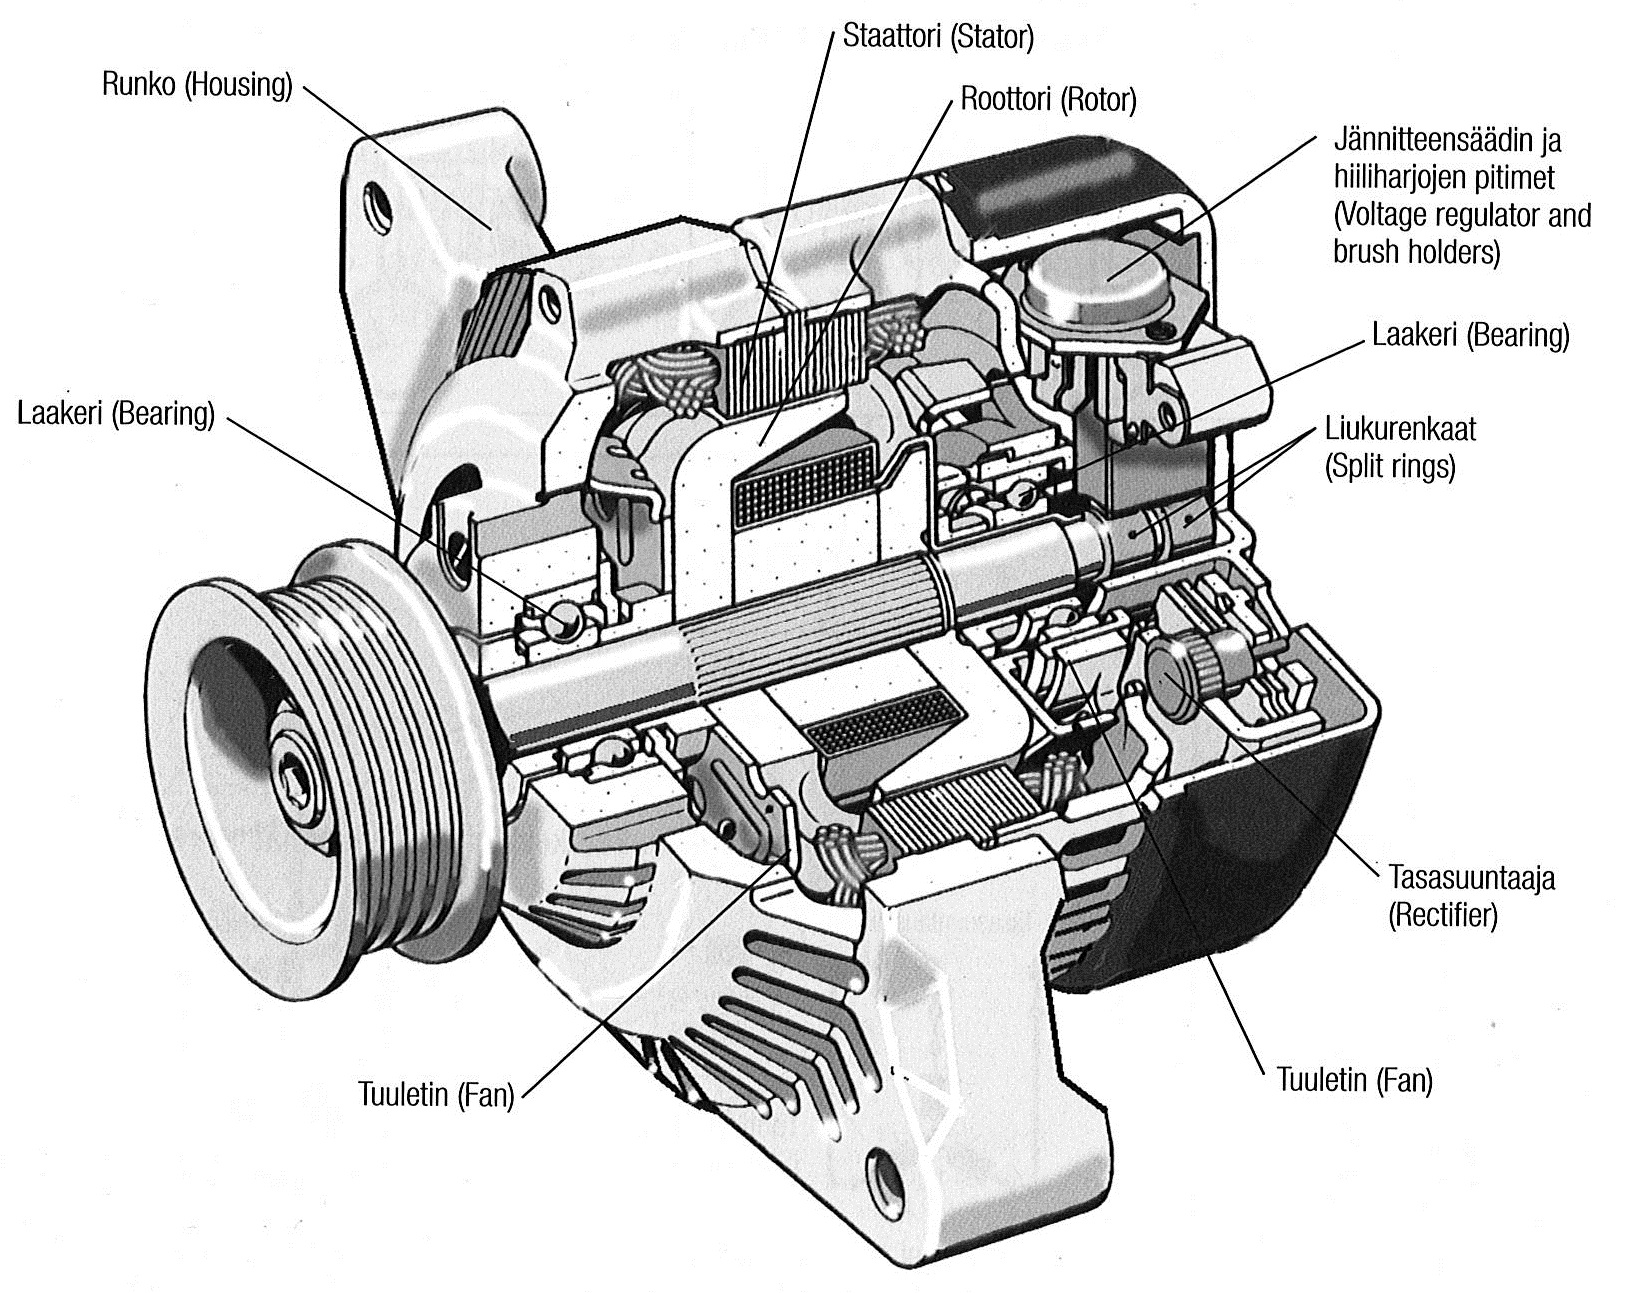
\includegraphics[height=80mm]{latausjarjestelma_pics/laturi.jpg}
\end{center}
\tiny Kuvan lähde: Simo Nieminen: {\em Auton sähkölaitteet}, 1. painos (2008), WSOY, sivu 131.
}

\frame{
\begin{center}
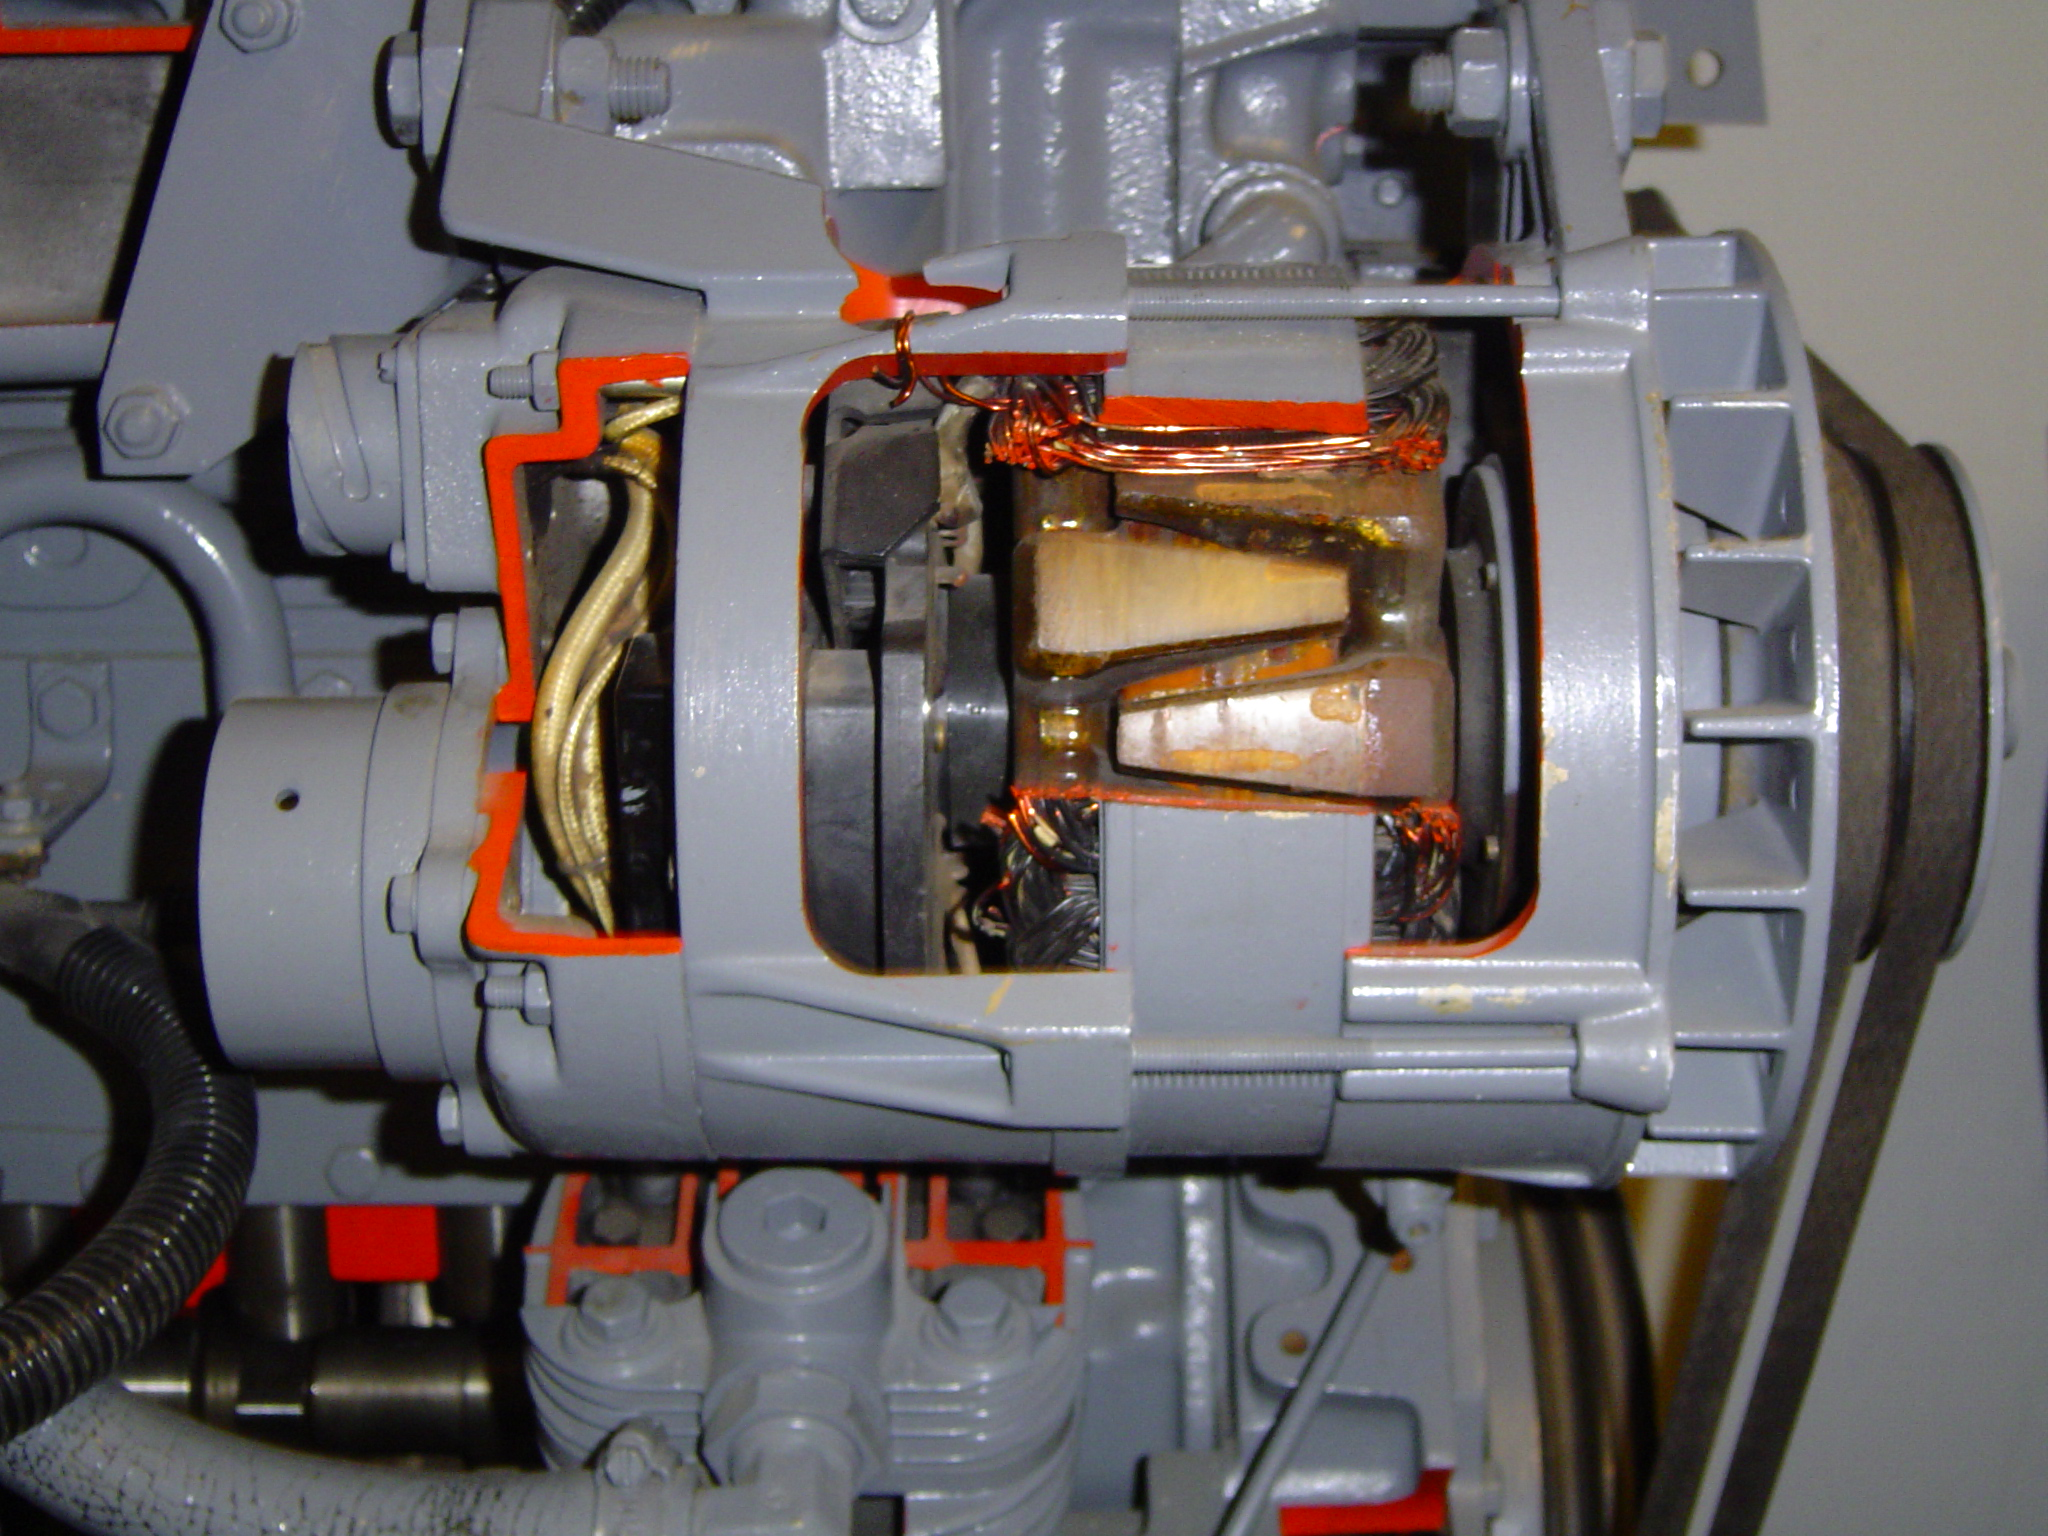
\includegraphics[height=80mm]{latausjarjestelma_pics/dynamo.jpg} % http://en.wikipedia.org/wiki/File:Dynamo.JPG
\end{center}
\tiny \url{http://en.wikipedia.org/wiki/File:Dynamo.JPG}
}

\frame{
\begin{center}
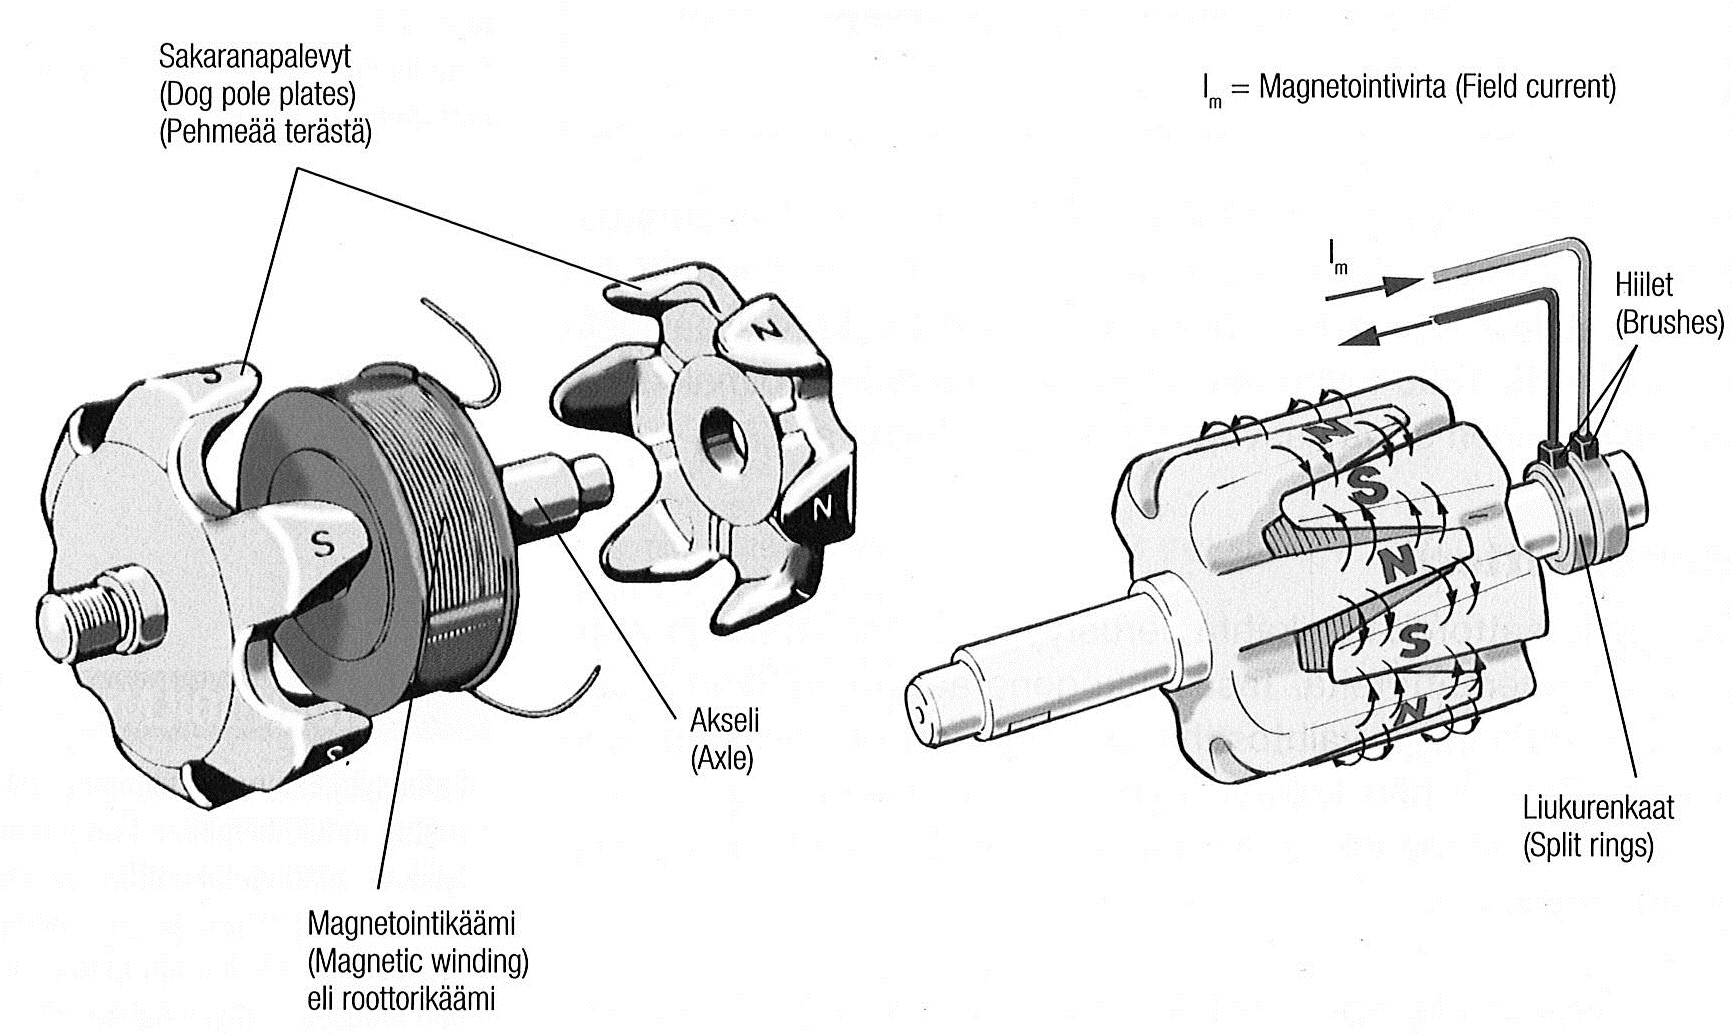
\includegraphics[height=70mm]{latausjarjestelma_pics/roottori.jpg}
\end{center}
\tiny Kuvan lähde: Simo Nieminen: {\em Auton sähkölaitteet}, 1. painos (2008), WSOY, sivu 130.
}

\frame{
\frametitle{Generaattorin rakenne}
\begin{itemize}
\item Roottorin rakenne on erittäin yksinkertainen, joten se ei rikkoudu suurista kierrosnopeuksista.
\item Latausvirta otetaan ulos staattorikäämeiltä. Käämit kytketään joko tähteen tai kolmioon.
\item Käämit on kytketty diodisiltaan, joka tasasuuntaa jännitteen tasajännitteeksi.
\end{itemize}
}

\frame{
\frametitle{Hyötysuhde}
\begin{itemize}
\item Vaihtovirtalaturin (+jännitteensäätimen) hyötysuhde on hieman yli 50 prosenttia.
\item Häviöitä aiheutuu esimerkiksi pyörrevirroista, johtimien resistansseista, kitkasta ja jäähdytyspuhaltimesta. 
\item Suurilla vakionopeudelle optimoiduilla generaattoreilla päästään lähes 100 prosentin hyötysuhteeseen.
\end{itemize}
}

\frame{
\frametitle{Esimerkki nelinapaisesta generaattorista}
\url{http://www.electricalknowledge.com/images/2Phase4poleGeneratorAnimatedDiagramSlow.gif}

}



\frame{
\frametitle{Jännitteensäädin}
\begin{itemize}
\item Periaate sama kuin missä tahansa säätöpiirissä.
\item Jos jännite meinaa nousta yli ohjearvon, kenttävirtaa pienennetään.
\item Jos jännite meinaa laskea alle ohjearvon, kenttävirtaa kasvatetaan.
\end{itemize}
}

\frame{
\frametitle{Jännitteensäädin}
\begin{itemize}
\item Oppikirjan sivulla 419 on esimerkki jännitteensäätimen kytkentäkaaviosta.
\item Uusia jännitteensäätimiä ohjataan usein digitaalisesti. Tämä mahdollistaa useita vikadiagnoositoimintoja, generaattorin
virrantuoton viivyttämisen moottoria käynnistettäessä sekä hidastetun latausvirran muutoksen (ei äkillisiä kuormituspiikkejä hihnalle).
\end{itemize}
}

\frame{
\begin{center}
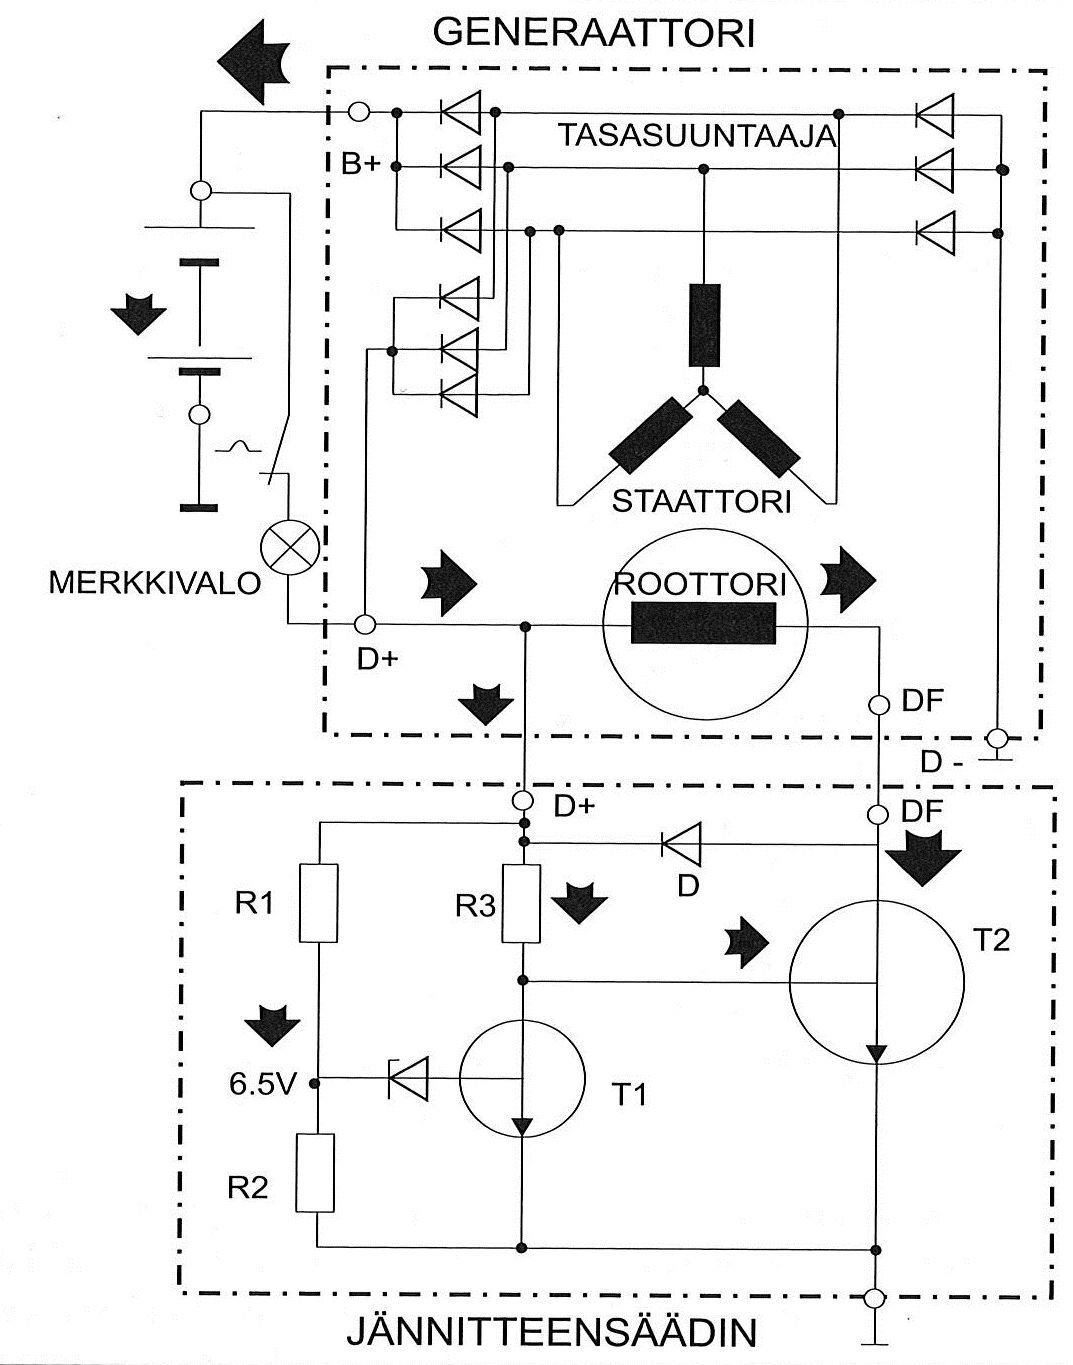
\includegraphics[height=80mm]{latausjarjestelma_pics/saadin.jpg}
\end{center}
\tiny Kuvan lähde: Juhala--Lehtinen--Suominen--Tammi: {\em Moottorialan sähköoppi}, 8. painos (2005), Autoalan koulutuskeskus, sivu 419.
}

\frame{
\frametitle{Mekaaninen jännitteensäädin}
\begin{itemize}
\item Vanhoissa generaattoreissa jännitteensäädin oli mekaaninen säädin, joka katkoi kenttävirtaa sopivasti.
\item Mekaaniset osat kuluvat nopeasti, siksi niistä pyritään eroon suunnittelussa.
\end{itemize}
}

\frame{
\frametitle{Liukurenkaaton generaattori}
\begin{itemize}
\item Generaattorin kuluvin osa on liukurenkaat hiiliharjoineen.
\item Liukurenkaattomassa generaattorissa magnetointikäämi on kytketty staattoriin, ja roottori toimii
ainoastaan magneettivuon ohjaimena.
\item Pienissä työkoneissa ja moottoripyörissä käytetään kestomagneettigeneraattoreita.
\item Kestomagneettigeneraattorin lähtöjännitettä säädetään pulssinleveysmodulaatiolla.
\end{itemize}
}

\frame{
\frametitle{Virranrajoitus}
\begin{itemize}
\item Sähkömagnetismiin perustuvan generaattorin virta rajoittuu luonnostaan johonkin maksimiarvoon, joten
erillistä suojapiiriä ei välttämättä tarvita.
\item Esimerkiksi pyörimisnopeuden kasvu kasvattaa jännitteen taajuutta, jolloin käämien induktanssi rajoittaa virtaa.
\end{itemize}
}

\frame{
\frametitle{Latausjärjestelmän huoltotoimenpiteet}
\begin{itemize}
\item Hihnan kireyden tarkastus.
\item Johtimien kunnon tarkastus.
\item Generaattorin puhdistus.
\item Hiilten vaihto.
\end{itemize}
}

\frame{
\frametitle{Akun varautumisen valvontajärjestelmä}
\begin{itemize}
\item Uusissa autoissa on jännitteensäätimen lisäksi akun varautumisen valvontajärjestelmä, joka seuraa muun muassa akun latausvirtaa. Virtatunnistin sijoitetaan esimerkiksi akkukenkään.
\item Valvontajärjestelmä muun muassa ottaa huomioon akun lämpötilan. Latausjännitettä voidaan nostaa kylmällä säällä reilusti yli 14
voltin, jos auton valot toimivat PWM-säädöllä. Tällöin polttimot eivät rikkoonnu.
\item Järjestelmä seuraa kokonaisvaltaisesti varaustilannetta ja kytkee lisälaitteita tarvittaessa pois päältä, tai nostaa tyhjäkäyntinopeutta.
\end{itemize}
}


\frame{
\frametitle{Vianhaku}
\begin{itemize}
\item Korjausoppaassa on kerrottu ohjearvot latausjärjestelmälle.
\item Latausjännite on tyypillisesti 13,8--14,4 volttia, kun kierrosluku on 2500 rpm.
\end{itemize}
}

\frame{
\frametitle{Vianhaku}
\begin{itemize}
\item Diodien ja käämien kunto on helppo testata yleismittarilla.
\item Yleismittarissa on erityinen dioditestaustoiminto, jolla voi mitata diodin kynnysjännitteen.
\item Kynnysjännite on yleensä 0,6...1 V päästösuuntaan. Estosuuntaan ehjä diodi ei johda.
\item Roottorikäämin resistanssi on yleensä muutamia ohmeja, staattorikäämeillä huomattavasti alle ohmin.
\end{itemize}
}

\frame{
\frametitle{Generaattorin merkinnät}
Bosch-generaattoreissa käytetään merkintöjä
\begin{itemize}
\item Vanha tapa: 14 V 35 A 24: nimellisjännite 14 V, maksimituotto 35 ampeeria ja se pyörintänopeus (2400 rpm), jolla
generaattori tuottaa 3/4 maksimivirrastaan.
\item Uusi tapa: 14 V 23/55 A: nimellisjännite sekä virrantuotot nopeudella 1500 rpm ja 6000 rpm.
\end{itemize}
}

\frame{
\frametitle{Käynnistysjärjestelmä}
Polttomoottori ei käynnisty "itsestään" kuten höyrykone tai sähkömoottori.
\begin{itemize}
\item Tarvittava vääntömomentti määräytyy moottorin koon, rakenteen ja lämpötilan mukaan.
\item Nelitahtiottomoottorit vaativat 60--120 rpm käynnistysnopeuden, kaksitahtiset noin 200 rpm.
\item Dieselmoottoreilla noin 100 rpm, kammiomoottoreilla 120--200 rpm.
\item Ajoneuvokäytössä olevat moottorit käytännössä aina sähkömoottorikäynnisteisiä.
\item Käynnistimien nimellistehot vaihtelevat 0,3 kW -- 6 kW.
\end{itemize}
}

\frame{
\frametitle{Perusrakenne}
Käynnistysjärjestelmän pääosat ovat
\begin{itemize}
\item akku
\item virtalukko
\item käynnistin.
\end{itemize}
}

\frame{
\frametitle{Käynnistimen rakenne}
\begin{itemize}
\item Käynnistin koostuu moottorista, magneettikytkimestä ja hammaspyörästä kytkentälaitteineen.
\item Moottori on yleensä sarjamoottori tai kestomagneettimoottori.
\item Sarjamoottorin rakenne on yksinkertainen ja se tuottaa suuren momentin päällekytkentätilanteessa.
\item Moottori on yleensä 4- tai 6-napainen.
\end{itemize}
}

\frame{
\begin{center}
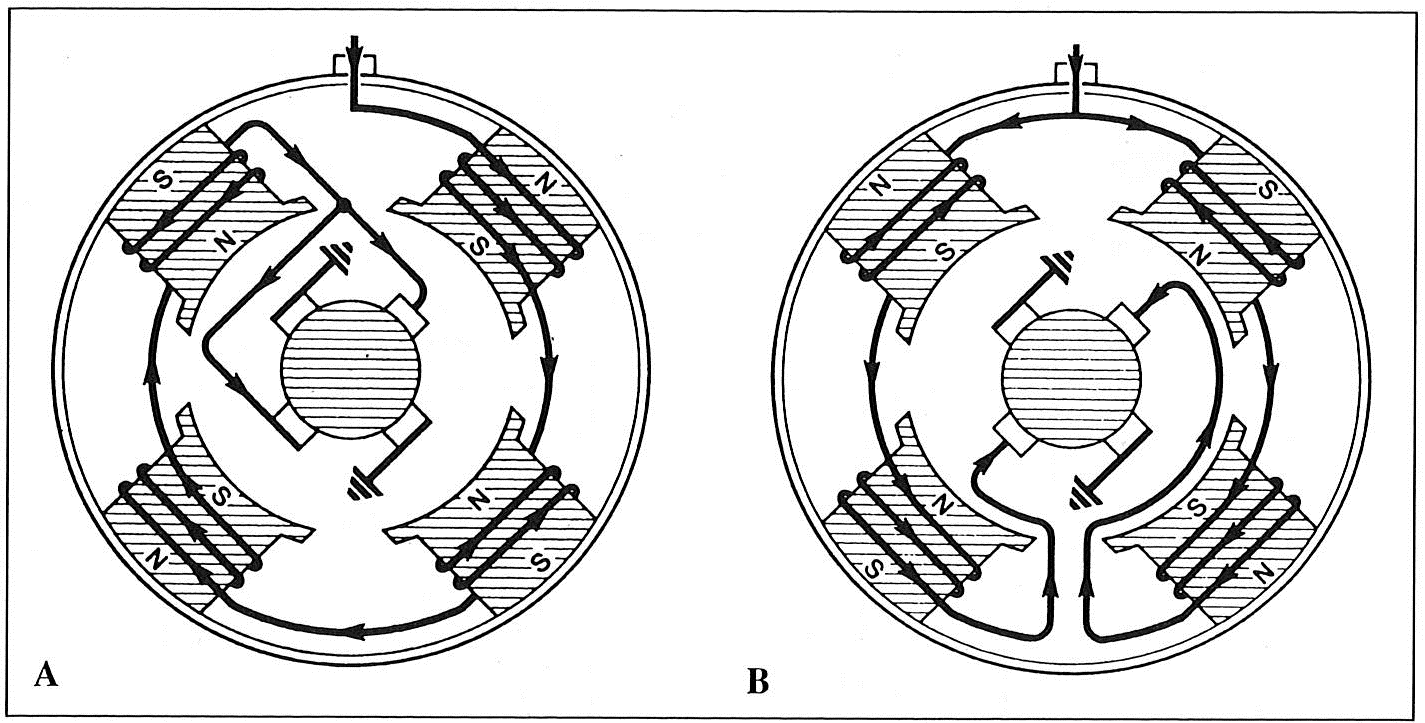
\includegraphics[height=60mm]{kaynnistysjarjestelma_pics/sarjamoottori.png}
\end{center}
\tiny Kuvan lähde: Juhala--Lehtinen--Suominen--Tammi: {\em Moottorialan sähköoppi}, 8. painos (2005), Autoalan koulutuskeskus, sivu 451.
}

\frame{
\frametitle{Hammaspyörien kytkentälaitteet}
\begin{itemize}
\item Käynnistinmoottorin akselilla oleva hammaspyörä pyörittää moottorin vauhtipyörällä olevaa hammaskehää.
\item Välityssuhde on tavallisesti 1:10--1:15.
\item Käynnistinmoottori kestää vain hyvin pieniä kierrosnopeuksia, joten se on pakko kytkeä irti moottorista käynnistyksen jälkeen.
\end{itemize}
}

\frame{
\frametitle{Hammaspyörien kytkentälaitteet}
Kolme päätyyppiä
\begin{itemize}
\item Magneettikytkimellä toimivat.
\item Käynnistimen hammaspyörän hitauteen perustuvat.
\item Siirtyvän ankkurin avulla toimivat.
\end{itemize}
}

\frame{
\frametitle{Kiertokäynnistin (vapaasiirtoinen kytkentähammaspyörä)}
\begin{itemize}
\item Perustuu hammaspyörän omaan hitauteen.
\item Käytetty vanhemmissa autoissa ja pienissä moottoreissa.
\item Kytkentähammaspyörä on kiinnitetty käynnistinmoottorin uritettuun akseliin.
\item Kun moottorin akseli pyörähtää, uritus työntää hammaspyörän akselin päähän ja kytkeytyy vauhtipyörään.
\item Kun moottori on käynnistynyt (=pyörii nopeammin kuin käynnistinmoottori), vauhtipyörän hammaskehä heittää 
hammaspyörän takaisin lähtöpaikkaansa.
\end{itemize}
}

\frame{
\frametitle{Työntökiertokäynnistin  (pakkosiirtoinen kytkentähammaspyörä)}
\begin{itemize}
\item Käytössä kevyessä ja keskiraskaassa kalustossa.
\item Magneettikytkin eli solenoidi työntää hammaspyörän vauhtipyörän hammaskehälle ja kytkee samalla käynnistinmoottoriin virran.
\item Hammasrattaan sisällä on vapaakytkin, joka suojaa käynnistysmoottoria rikkoontumasta välittömästi käynnistyksen jälkeen.
\end{itemize}
}

\frame{
\begin{center}
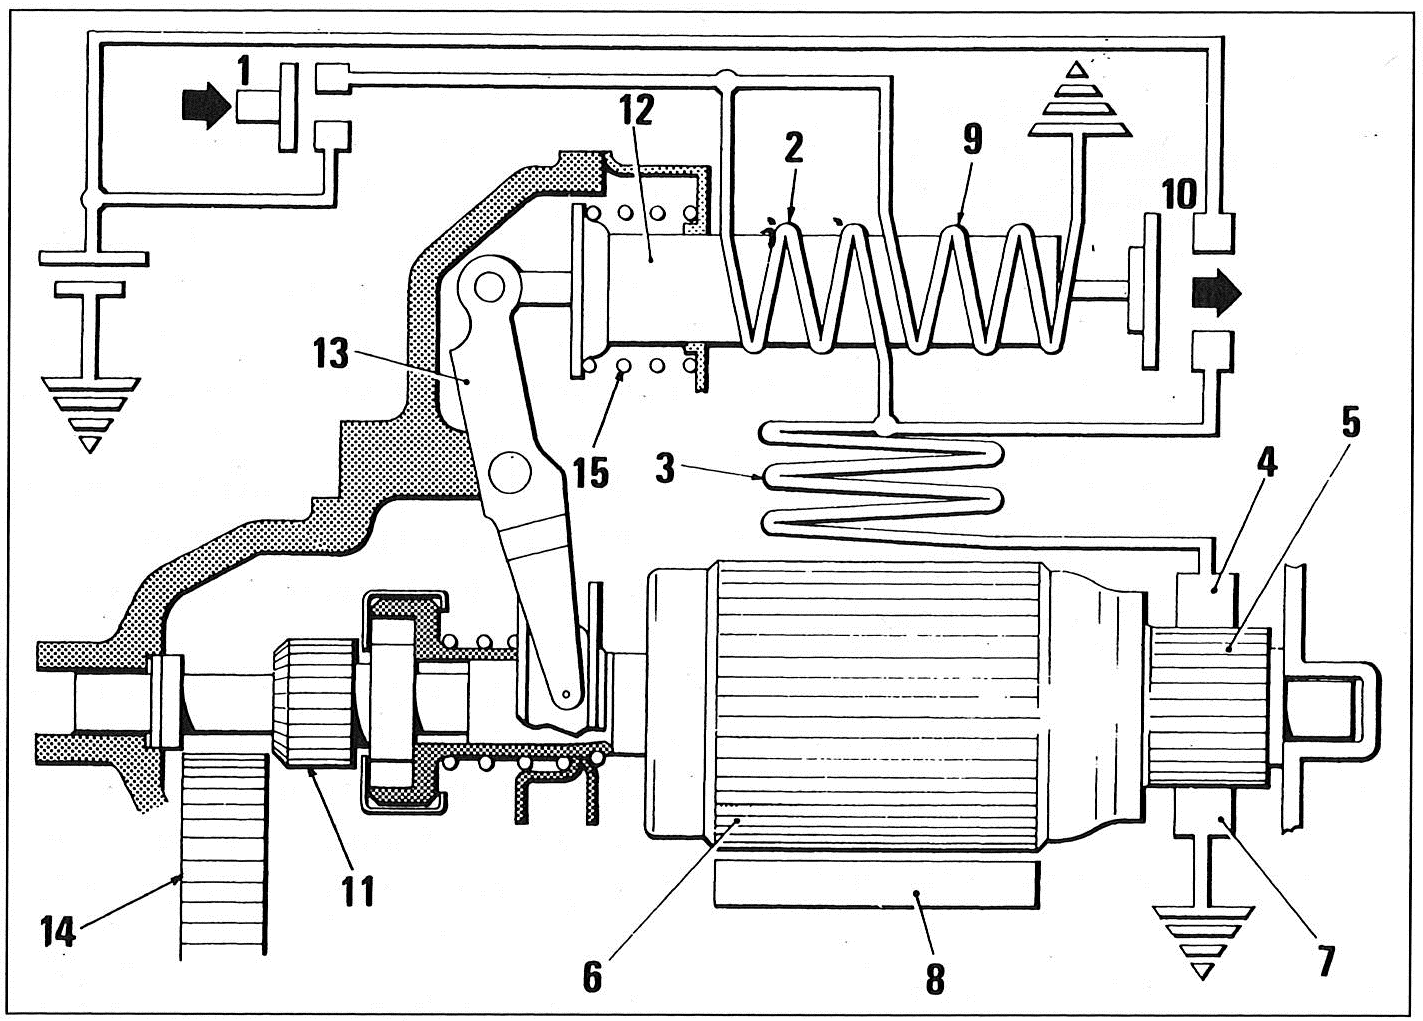
\includegraphics[height=80mm]{kaynnistysjarjestelma_pics/tyontokierto.png}
\end{center}
\tiny Kuvan lähde: Juhala--Lehtinen--Suominen--Tammi: {\em Moottorialan sähköoppi}, 8. painos (2005), Autoalan koulutuskeskus, sivu 453.
}

\frame{
\begin{center}
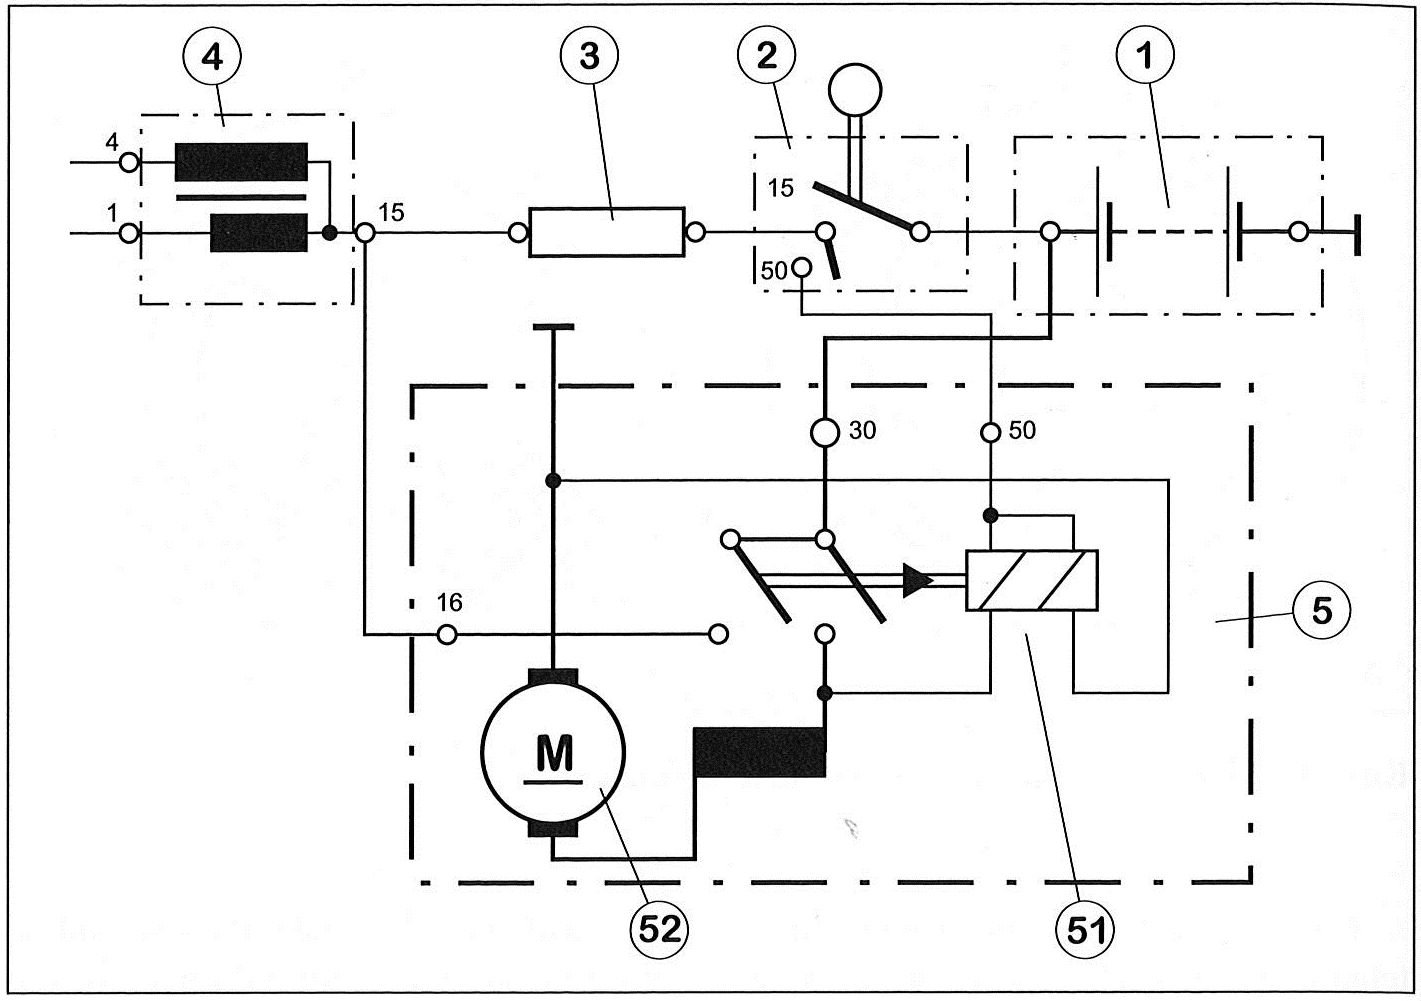
\includegraphics[height=80mm]{kaynnistysjarjestelma_pics/kytkis.png}
\end{center}
\tiny Kuvan lähde: Juhala--Lehtinen--Suominen--Tammi: {\em Moottorialan sähköoppi}, 8. painos (2005), Autoalan koulutuskeskus, sivu 452.
}

\frame{
\begin{center}
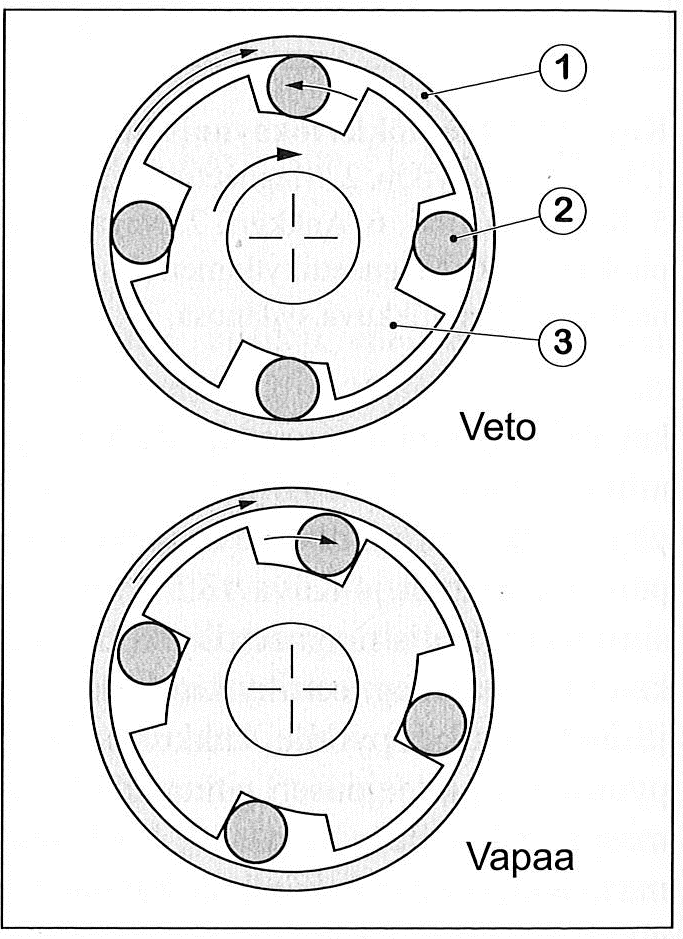
\includegraphics[height=80mm]{kaynnistysjarjestelma_pics/vapaak.png}
\end{center}
\tiny Kuvan lähde: Juhala--Lehtinen--Suominen--Tammi: {\em Moottorialan sähköoppi}, 8. painos (2005), Autoalan koulutuskeskus, sivu 454.
}

\frame{
\frametitle{Raskaan kaluston käynnistimet}
\begin{itemize}
\item Raskaissa dieselmoottoreissa vääntömomentin tarve on erittäin suuri.
\item Nykyään raskaassa kalustossa käytetään usein samaa tekniikkaa kuin pienemmissäkin moottoreissa.
\item Vanhemmissa kuorma-autoissa käynnistiminä käytettiin {\em työntöankkurikäynnistintä} ja {\em työntökäynnistintä}.
\item Keskiraskaissa moottoreissa käytetään {\em työntöankkurikäynnistintä}, joka toimii kuten työntökiertokäynnistin,
mutta siirtyvänä osana on koko moottorin ankkuri.
\item Hyvin suurilla käynnistystehoilla käytetään {\em työntökäynnistintä}, jossa solenoidi työntää onton akselin sisällä kulkevaan
tankoon kiinnitetyn hammaspyörän hammaskehäkosketukseen. Järjestelmässä on myös oma lamellikytkin, joka suojelee ankkuria
liian suurelta pyörimisnopeudelta ja momentilta.
\end{itemize}
Raskaat dieselmoottorit voidaan käynnistää myös paineilmalla, pienellä polttomoottorilla tai räjähdyspanoksella.
}

\frame{
\frametitle{Kestomagnetoitu käynnistin}
\begin{itemize}
\item Uusien voimakkaiden magneettien valmistustekniikan kehittyminen mahdollistaa kenttäkäämien
korvaamisen kestomagneeteilla. Etu: pienempi koko ja keveys.
\item Vääntömomentti on heikompi; tämä voidaan kompensoida pienellä vaihteistolla.
\end{itemize}
}

\frame{
\frametitle{Käynnistin-generaattori}
\begin{itemize}
\item Sama laite toimii sekä käynnistimenä että generaattorina.
\item Käytössä 50-70 -luvun pikkuautoissa, skoottereissa ja veneissä nimellä Dynastart.
\item Nykyään sama periaate hybridiautoissa: moottorin ja vaihteiston väliin on asennettu kestomagneettimoottori,
joka toimii myös vauhtipyöränä.
\item Ohjaus täysin elektroninen. Käyttöjännitteet vaihtelevat muutamista kymmenistä volteista aina 500 volttiin asti.
\end{itemize}
}


\frame{
\frametitle{Käynnistimen koestaminen}
Irrotettu käynnistin voidaan koestaa koestuslaitteessa.
\begin{itemize}
\item Joutokäyntikoe: käynnistimelle syötetään virtaa kuormittamattomana. Kuunnellaan sivuääniä ja luetaan virta ja jännite.
\item Kuormituskoe käynnistysnopeudella: käynnistintä jarrutetaan niin, että se pyörii käynnistysnopeudella. Tarkistetaan, että
jännite ja virta pysyvät ohjearvoissa.
\item Kuormituskoe lukittuna: käynnistin jarrutetaan pysähdyksiin ja luetaan jännite ja virta.
\end{itemize}
Kestomagneettimoottori voi tuhoutua jos se jarrutetaan lukkoon. Noudata aina valmistajan koestusohjeita.
}

\frame{
\frametitle{Käynnistimen kunnostus}
\begin{itemize}
\item Käynnistimen perusrakenne on yksinkertainen. Kunnostus ei eroa generaattorin kunnostamisesta: hiiliharjat, harjajouset ja käämitykset voidaan uusia.
\item Usein pääsee vähimmällä uusimalla koko käynnistimen.
\item Vauhtipyörän hammaskehä on tavallisesti kiinnitetty kutisteliitoksella ja se on vaihdettavissa.
\end{itemize}
}

\frame{
\frametitle{Dieselmoottorin hehkutuslaitteet}
\begin{itemize}
\item Vanhoissa autoissa hehkutus tapahtui erillisellä hehkutuskytkimellä.
\item 1970-luvulla käyttöön mekaanisella tai elektronisella lämpötilatunnistimella varustetut releet.
\item Nykyiset järjestelmät täysin elektronisesti ohjattuja.
\item Hehkutus voi alkaa jo, kun ovi avataan tai avain työnnetään virtalukkoon.
\item 2000-luvulla hehkutusrele korvattu tehotransistoreilla $\to$ pwm-säätö. Lisäksi tulppia ohjataan yksitellen.
\end{itemize}
}


\frame{
\frametitle{Hehkutusjärjestelmän vianhaku}
\begin{itemize}
\item Viallinen hehkutulppa on helppo löytää pihtivirtamittarin avulla.
\item Tulpan riittävä jännitteensaanti voidaan varmistaa mittaamalla akun plusnavan ja tulpan välinen jännite. Toimivassa järjestelmässä se on alle 1 V.
\end{itemize}
}

\frame{
\frametitle{Jäähdytysnesteen lämmittäminen hehkutulpilla}
\begin{itemize}
\item Uusissa etenkin pienikokoisissa dieselmoottoreissa terminen hyötysuhde voi olla niin hyvä, että jäähdytysnesteen lämpötila voi sopivissa olosuhteissa  jäädä niin alhaiseksi, että auton lämmityslaite ei toimi kunnolla.
\item Ongelma voidaan ratkaista lämmittämällä jäähdytysnestettä hehkutulppien avulla. Käytössä on myös polttoainekäyttöisiä lisälämmittimiä.
\item Lisälämmitys auttaa moottoria saavuttamaan toimintalämpötilansa nopeammin kylmäkäynnistyksen jälkeen.
\end{itemize}
}

% Kirjasta Nieminen: Auton sähkölaitteet sivu 154...
\frame{
\frametitle{Start-Stop -automatiikka}
\begin{itemize}
\item Kaupunkiajossa liikennevaloissa seisominen saastuttaa turhaan ilmaa ja kuluttaa polttoainetta.
\item Ratkaisu: pysäytetään moottori liikennevaloissa. Automatiikan tulee olla erittäin toimintavarma.
\item Start-Stop -järjestelmä pysäyttää moottorin, kun auto seisoo paikallaan, vaihde on vapaalla ja kytkinpoljin ylhäällä.
\item Kytkinpolkimen painaminen käynnistää moottorin välittömästi, jolloin autolla pääsee sujuvasti liikkelle.
\item Käynnistykseen voidaan käyttää myös generaattoria (lämmin moottori vaatii pienemmän momentin).
\item Start-Stop -järjestelmä voi vähentää polttoaineenkulutusta kaupunkiajossa yli 10 \%.
\end{itemize}
}

\frame{
\frametitle{Suorakäynnistys}
\begin{itemize}
\item Nykyaikainen suorasuihkutusmoottori on mahdollista käynnistää ilman käynnistintä.
\item Moottorinohjausjärjestelmä valitsee sylinterin, jossa mäntä on pysähtynyt sopivaan asentoon (työtahdin alkuosa).
\item Sylinteriin suihkutetaan polttoainetta ja annetaan kipinä => moottori pyörähtää käyntiin.
\item Esim. Mazda SISS (Smart Idle Stop System).
\end{itemize}
}
% OSA KALVOISTA LAINATTU MOOTTORINOHJAUSKURSSILTA, K2010 LUENTO 4

\frame{
\frametitle{Sytytysjärjestelmä}
Ottomoottorissa polttoaine-ilmaseos sytytetään suurjännitekipinällä. Sytytysjärjestelmän tehtävä on sytyttää ilma-polttonesteseos
\begin{itemize}
\item oikealla hetkellä (optimaalinen suorituskyky ja päästöt)
\item luotettavasti (HC-päästöt, käyntihäiriöt).
\end{itemize}
}

\frame {
\frametitle{Sytytysjärjestelmä}
Sytytysjärjestelmän perusperiaate pysynyt samana 1800-luvun lopulta asti: ilman ja polttoaineen seos
sytytetään sähkökipinällä. Moottorinohjauksella vaikutetaan {\bf sytytyshetkeen}.
Sytytyshetken valinta vaikuttaa seuraaviin asioihin
\begin{itemize}
\item moottorista ulos saatava teho
\item polttonesteen kulutus
\item nakuttaako moottori vai ei
\item kuinka puhtaita ovat pakokaasut
\end{itemize}
Kaikkia asioita ei saada parhaaseen mahdolliseen arvoon samanaikaisesti, vaan on tehtävä kompromissi.
Esimerkiksi sytytyksen aikaistaminen lisää moottorin tehoa ja vähentää kulutusta, mutta lisää hiilivety- (HC) ja
typenoksidipäästöjä (NO$\rm _x$).
}

\frame{
\frametitle{Nykyaikainen sytytyksenohjausjärjestelmä}
\begin{itemize}
\item 2000-luvun autoissa sytytyksenohjausyksikkö on integroitu samaan pakettiin polttoaineensuihkutuksen
ohjausyksikön kanssa.
\item ECU = engine control unit.
\item "Kaikki vaikuttaa kaikkeen"
\item Vanhanaikaisiin sytytysjärjestelmiin tutustuminen on kuitenkin havainnollista.
\end{itemize}
}




\frame{
\frametitle{Sytytystulpat}
\begin{itemize}
\item Tulpan elektrodien väliin syttyvä valokaari sytyttää polttoaineilmaseoksen.
\item Tulpan on kestettävä kemiallista rasitusta, korkeita lämpötiloja (jopa 1000 $^\circ$C), korkeita jännitteitä (30 kV)
ja korkeaa painetta (80 bar).
\item Sytytystulppien käyttölämpötilan on oltava suurin piirtein välillä 500 $^\circ$C - 900 $^\circ$C. Liian kylmässä tulppa
ei pala puhtaaksi (oikosulkuvaara), ja liian kuuma lämpötila johtaa voimakkaaseen korroosioon ja hehkusyttymisen vaaraan.
\item Tulpan {\bf lämpöarvo} kertoo, kuinka paljon tulppa lämpenee. Pienen (2...5) lämpöarvoluvun tulppiin johtuu vähän
lämpöä palotilasta. Suuren (7...10) lämpöarvoluvun tulppiin johtuu paljon lämpöä.
\item Väärien tulppien käyttö johtaa esimerkiksi karstoittumiseen (liian kylmät tulpat) tai korroosioon (liian kuumat tulpat).
\end{itemize}
}

\frame{
\frametitle{Sytytysjärjestelmien perusrakenteet}
\begin{itemize}
\item Induktiivinen ja kapasitiivinen akkusytytys.
\item Induktiivinen ja kapasitiivinen magneettosytytys.
\end{itemize}
}

\frame{
\frametitle{Induktiivisten sytytysjärjestemien päätyypit}
\begin{tabular}{ l l p{6cm} }
 & Nimi & Ominaisuudet\\
SZ & Puolasytytys & Sytytysimpulssi, säätö ja kipinänjako mekaanisesti.\\
TZ & Transistorisytytys& Impulssi tuotetaan elektronisesti.\\
EZ & Elektroninen sytytys& Impulssi ja säätö elektronisesti.\\
VZ & Täyselektroninen sytytys& Sytytysimpulssi, säätö ja kipinänjako elektronisesti.\\
\end{tabular}

}

\frame{
\begin{center}
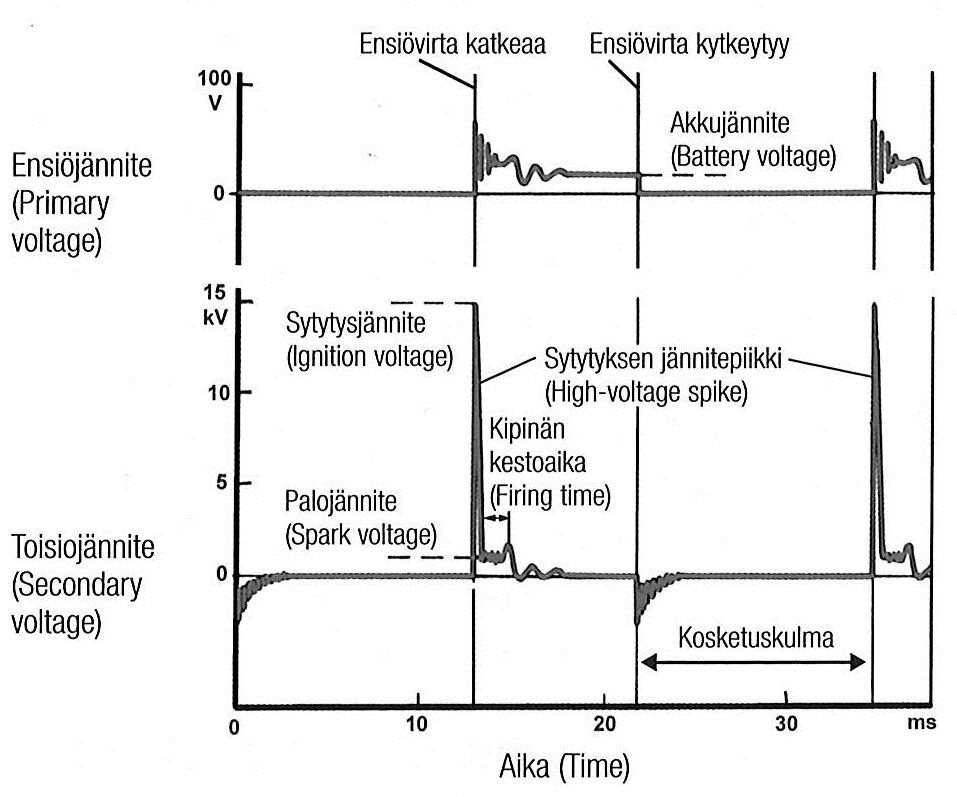
\includegraphics[height=80mm]{sytytysjarjestelma_pics/kayra.png}
\end{center}
\tiny Kuvan lähde: Simo Nieminen: {\em Auton sähkölaitteet}, 1. painos (2008), WSOY, sivu 195.
}

\frame{
\frametitle{Wanhanaikainen puolasytytys (SZ)}
\begin{itemize}
\item Sytytysimpulssi tuotetaan katkaisemalla sytytyspuolan virta katkojan kärjillä.
\item Kun kärjet ovat kiinni, puolan ensiökäämin virta kasvaa (energiaa varastoituu magneettikenttään).
\item Kun virta katkaistaan äkillisesti, toisiokäämiin indusoituu korkeajännite, joka aikaansaa kipinän tulpan kärkien välillä.
\item Suurilla kierrosluvuilla ensiövirta ehtii olla kytkettynä vain vähän aikaa. Magneettikenttään varastoituu vähemmän
energiaa kuin pienillä kierrosluvuilla.
\item Ensiökäämin induktanssin on oltava riittävän pieni, jotta myös suurilla kierrosluvuilla syntyy riittävän suuri jännite.
\item Virtaa rajoitetaan usein etuvastuksella, joka ohitetaan kylmäkäynnistyksessä.
\end{itemize}
}

\frame{
\begin{center}
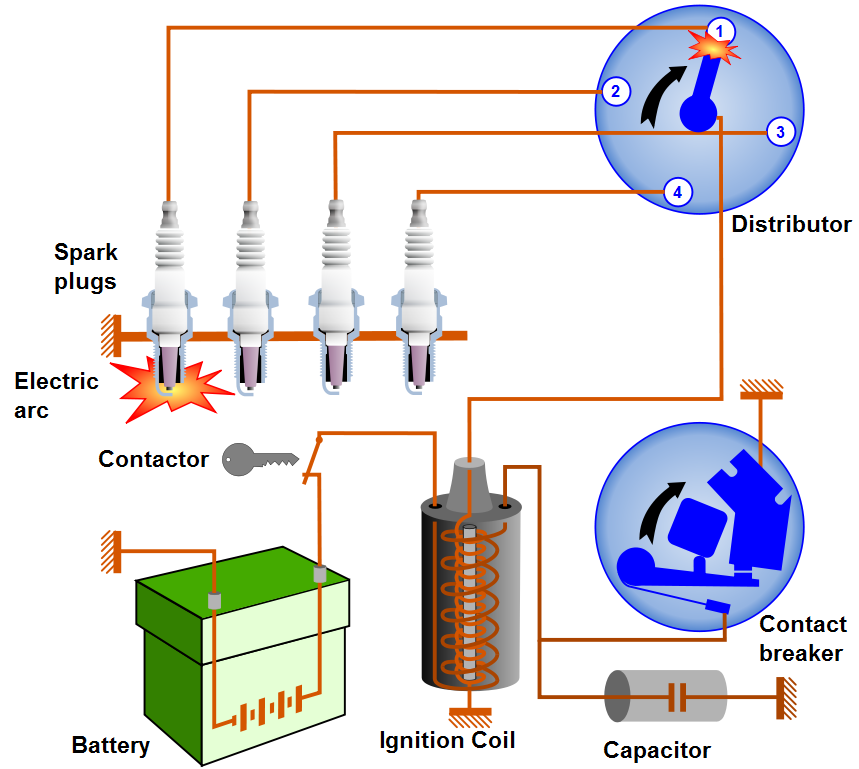
\includegraphics[height=60mm]{sytytysjarjestelma_pics/perus.png}
\end{center}
\tiny Kuvan lähde: \url{http://commons.wikimedia.org/wiki/File:Car_ignition_system.svg}
}


\frame{
\frametitle{Virranjakaja}
\begin{itemize}
\item Virranjakajan tehtävä on jakaa jännitepulssi oikealle tulpalle.
\item Katkojan tehtävä on katkaista ensiövirta oikealla hetkellä (SZ).
\item Nykyaikaisissa sytytys- ja moottorinohjausjärjestelmissä virranjakaja huolehtii ainoastaan
kipinän jakamisesta tulpille.
\item Täyselektronisissa järjestelmissä mekaanista virranjakajaa ei tarvita.
\end{itemize}
}

\frame{
\frametitle{Katkoja}
\begin{itemize}
\item Katkojassa on nokan käyttämä kosketinkärki, joka katkaisee ensiövirran.
\item Kuluva osa, sekä mekaanisesti että kipinöinnin takia (virran katkaiseminen aikaansaa kipinän
myös ensiöpuolella).
\item Sytytyskondensaattori vähentää kipinöintiä ja radiotaajuisia häiriöitä.
\end{itemize}
}

\frame{
\frametitle{Keskipako- ja alipainesäädin}
\begin{itemize}
\item SZ- ja TZ-järjestelmissä virranjakajaan on integroitu säätimet, jotka säätävät sytytysennakkoa
moottorin kuorman ja kierrosluvun mukaan.
\item Keskipakosäädin säätää sytytystä sitä aikaisemmaksi, mitä suurempi on moottorin kierrosluku.
\item Alipainesäädin säätää sytytysennakkoa moottorin kuormituksen mukaan. Pienellä kuormituksella
ennakkoa kasvatetaan, koska seos palaa silloin hitaammin. 
\end{itemize}
}

\frame{
\frametitle{Transistorisytytysjärjestelmä (TZ)}
\begin{itemize}
\item Ero SZ-järjestelmään: ensiövirtaa ei katkota kärkiä läpsyttämällä, vaan elektronisesti.
\item On olemassa myös kärkiohjattuja transistorisytytysjärjestelmiä (TSZ-k), missä kärjet toimivat
anturina mutta varsinainen katkominen tapahtuu transistorin avulla.
\item Käytetyimmät anturityypit ovat induktiivinen impulssianturi (TZ-I) sekä Hall-anturi (TZ-H).
\item Etuja:
\begin{itemize}
\item Ensiövirran rajoitus voidaan tehdä elektronisesti (ei etuvastuksia ym.).
\item Kosketuskulman (kauanko ensiövirta on kytkettynä ennen kipinää) elektroninen säätö.
\item Lepovirran katkaisu (puola ei kuumene, jos moottori on sammutettu mutta sytytysvirta päällä).
\item Ei kuluvia kärkiä.
\end{itemize}

\end{itemize}
}


\frame{
\frametitle{Anturit}
\begin{itemize}
\item Moottorin asentoa mittaavasta sytytysjärjestelmän anturista käytetään myös termiä tahdistin.
\item Anturi voi sijaita virranjakajassa, vauhtipyörän yhteydessä tai kampiakselin etupäässä.
\item Induktiotahdistin: toimii kuten pieni sähkömoottori. Sijoitus virranjakajaan tai vauhtipyörälle.
\item Voidaan käyttää myös Hall-anturiin perustuvaa tahdistinta tai optista tahdistinta.
\end{itemize}
}

\frame{
\begin{center}
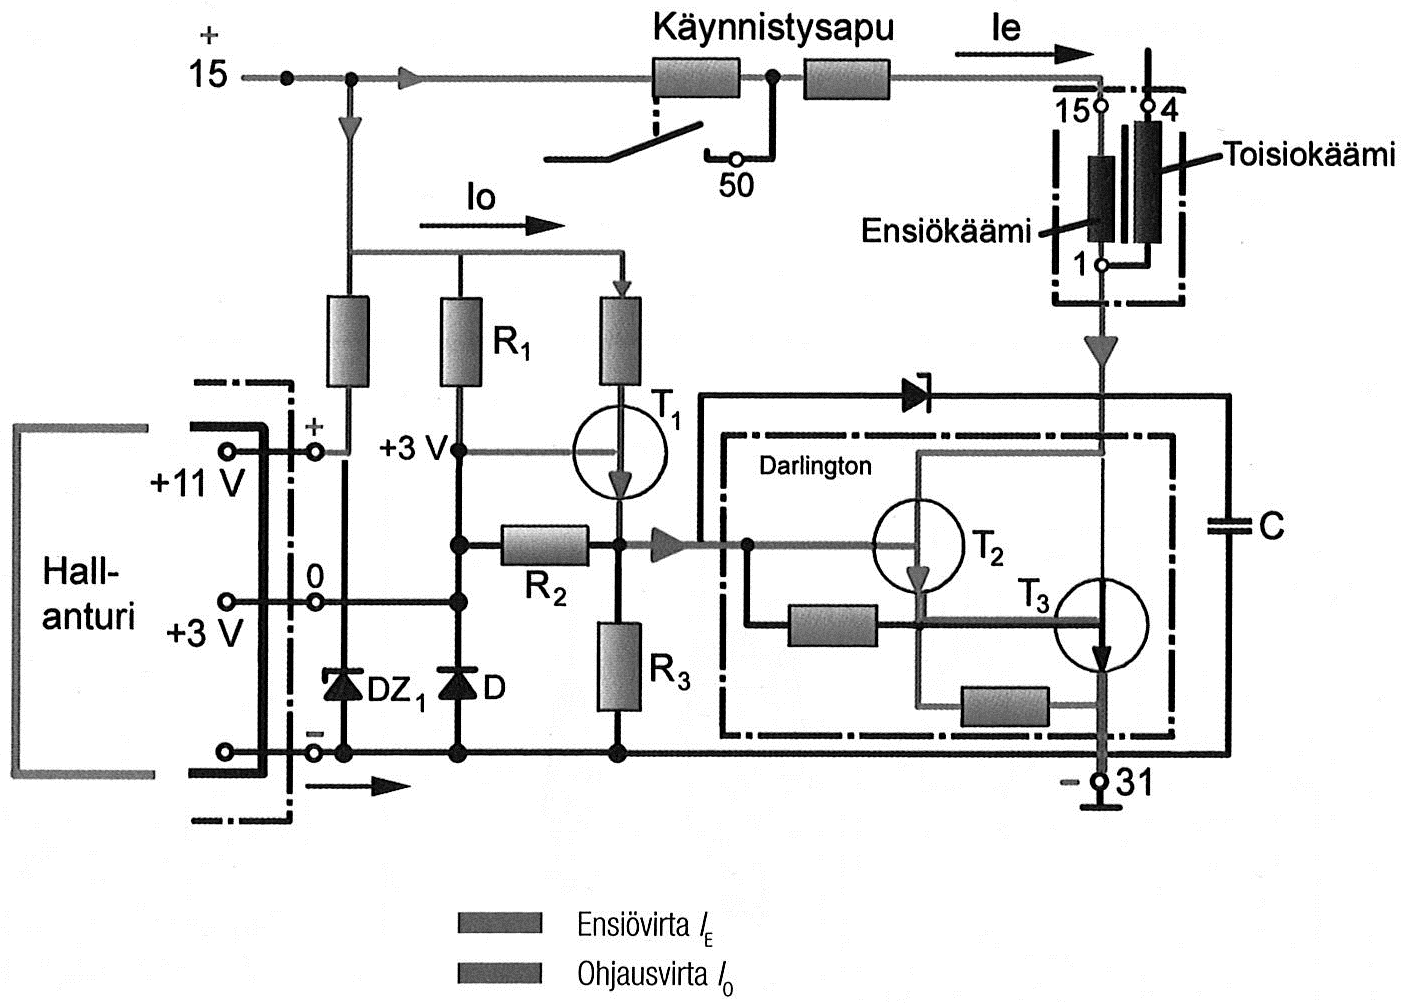
\includegraphics[height=80mm]{sytytysjarjestelma_pics/elektroninen.png}
\end{center}
\tiny Kuvan lähde: Simo Nieminen: {\em Auton sähkölaitteet}, 1. painos (2008), WSOY, sivu 200.
}


\frame{
\frametitle{Elektroninen sytytys (EZ)}
\begin{itemize}
\item Ero TZ-järjestelmään: alipaine- ja keskipakosäädin on korvattu elektronisella säätöyksiköllä.
\item Elektroniikan käyttö mahdollistaa mielivaltaiset säätökäyrästöt.
\item Tietokone laskee oikean sytytyshetken pyörintänopeuden, imusarjan paineen, moottorin ja imuilman lämpötilan ja
akkujännitteen perusteella.
\end{itemize}
}

\frame{
\frametitle{Täyselektroninen sytytys (VZ)}
\begin{itemize}
\item Ero EZ-järjestelmään: virranjakaja korvattu elektronisella kipinänjaolla.
\item Käyttö joko kaksoiskipinäsytytyspuolilla (kipinä sekä puristustahdissa että poistotahdissa olevalle sylinterille) tai
yksittäiskipinäsytytyspuolilla.
\end{itemize}
}

\frame{
\frametitle{Nakutuksen esto}
\begin{itemize}
\item Nakutus = polttoaine syttyy sekä itsestään että kipinästä. Kaksi palamisrintamaa kohtaavat $\to$ paineisku.
\item Nakutus voi tuhota moottorin muutamassa minuutissa.
\item Sytytysennakkoa säädettäessä on jätettävä turvaväli moottorin nakutusrajaan (=ennakko, jolla moottori todennäköisesti nakuttaa).
\item Käyttämällä elektronista nakutuksen tunnistinta, voidaan turvaväliä kaventaa huomattavasti. Nakutukseen voidaan reagoida
välittömästi ($\to$ sytytystä myöhäisemmälle).

\end{itemize}
}



\frame{
\frametitle{Kapasitiivinen sytytys (HKZ)}
\begin{itemize}
\item Kapasitiivisessa sytytysjärjestelmässä sytytysenergiaa ei varata sytytyspuolan käämiin, vaan
kondensaattoriin.
\item Sytytysmuuntajaa tarvitaan edelleen jännitteen nostoa varten.
\item Muuntajan ensiökäämin induktanssi on pieni, jotta energia purkautuu ensiökäämiin nopeasti.
\end{itemize}
}

\frame{
\frametitle{Kapasitiivisen sytytyksen ominaisuuksia}
\begin{itemize}
\item Kondensaattorin varaaminen kestää vain satoja mikrosekunteja $\to$ vahva kipinä myös suurilla käyntinopeuksilla.
\item Lyhyempi kipinän kestoaika; voidaan kompensoida jännitettä ja kärkiväliä kasvattamalla.
\item Tulpan kestoikä pitenee.
\item Suuri jännite lisää läpilyöntiherkkyyttä (kosteus, lika, kuluminen).
\item Monimutkaisempi ja kalliimpi kuin induktiivinen sytytysjärjestelmä.
\end{itemize}
}

\frame{
\frametitle{Toimintaidea}
\begin{itemize}
\item Kondensaattori ladataan 300--500 V jännitteeseen vaihtosuuntaaja--muuntaja--tasasuuntaaja -rakenteen avulla.
\item Kipinän antaminen tapahtuu purkamalla kondensaattori muuntajan ensiökäämin läpi käyttämällä kytkimenä esimerkiksi tyristoria
(tämän takia järjestelmää kutsutaan joskus tyristorisytytysjärjestelmäksi).
\end{itemize}
}

\frame{
\frametitle{Sytytysenergia}
Kondensaattorin kapasitanssi on noin 1 $\uF$. Jos se varataan 300 voltin jännitteeksi, on sytytykseen käytettävissä energiaa
\[
E=\frac{1}{2}CU^2=45\,{\rm mJ}.
\]
}

\frame{
\frametitle{Jakajaton kapasitiivinen sytytys}
\begin{itemize}
\item Jokaisella tulpalla oma pienoissytytysjärjestelmä muuntajineen ja kondensaattoreineen.
\end{itemize}
}

\frame{
\frametitle{Kapasitiivinen magneettosytytys}
\begin{itemize}
\item Perusperiaate sama kuin kapasitiivisessa akkusytytyksessä, mutta kondensaattorin varausenergia otetaan vauhtipyörämagneeton käämistä.
\end{itemize}
}

\frame{
\frametitle{Turvallisuus}
\begin{itemize}
\item Sytytysjärjestelmästä on mahdollista saada sähköisku.
\item Vaaralliset sähkötapaturmat harvinaisia; yksittäinen korkeajännitepulssi ei ole yhtä vaarallinen kuin valtakunnanverkon 50 Hz vaihtojännite.
\item Puolan toisiopuolta ei silti kannata sorkkia, jos sytytysvirta on kytketty (varsinkin vanhoissa järjestelmissä).
\item Uusissa järjestelmissä sytytysmuuntaja on kiinni suoraan tulpan kannassa. Tämä vähentää rf-häiriöitä ja siinä ohessa
lisää turvallisuutta (pitää olla todella sählä, että saa sähköiskun).
\end{itemize}
}

% HUOM! ANTURIKALVOISTA SUURI OSA LAINATTU MOOTTORINOHJAUKSEN K2010 LUENTO6 JA
% VÄYLÄKALVOT LUENTO8.



\frame{
\frametitle{Anturin määritelmä}
\begin{itemize}
\item Anturi on laite, joka muuttaa jonkin suureen (esimerkiksi kemiallisen tai fysikaalisen)  käsiteltävään muotoon
(jännitteeksi, virraksi, digitaaliseksi signaaliksi\ldots).
%\item
\end{itemize}
}


\frame{
\frametitle{Moottorinohjausjärjestelmän anturit}
\begin{description}
\item[1950-luku] $\lambda$-happianturi 
\item[1960] sähkömekaaninen paineanturi, pietsosähköinen nakutusanturi
\item[1970] hall-anturi, turvatyynyn venymäliuska-anturi, silikonipaineanturi
\item[1980] kuumalanka- ja ohutkalvoilmamassamittarit, integroitu paineanturi
\item[1990] mems-kiihtyvyysanturit, pietsosähköinen kiertonopeusanturi, mikromekaaninen
ilmamassa-anturi, mikromekaaninen kiertonopeusanturi

\end{description}
}



\frame{
\frametitle{Älykkäät anturit}
\begin{itemize}
\item Anturilta tulevan signaalin käsitteleminen tapahtuu itse anturiyksikössä.
\item Älykäs anturi voidaan kalibroida automaattisesti, käyttämällä useita antureita yhtäaikaa.
\item Suorittamalla signaalinkäsittely paikan päällä anturissa, moottorinohjausyksiköltä
vaaditaan vähemmän laskentatehoa.
\item Anturiliitäntä voidaan standardoida.
\end{itemize}
}

\frame{
\frametitle{Merkitys autotekniikassa}
\begin{itemize}
\item Sähkö- ja elektroniikkajärjestelmän osuus ajoneuvon arvosta on noin 26 \%.
\item Maailmassa valmistettavista antureista noin joka toinen sijoitetaan ajoneuvoon.
\end{itemize}
}

\frame{
\frametitle{Luotettavuus}
\begin{itemize}
\item Vikataajuus ilmoitetaan todennäköisyytenä, yksikkönä yleensä ppm/aikayksikkö.
\item Eli monenko miljoonasosan todennäköisyydellä anturi hajoaa aikayksikön aikana.
\item Ajoneuvoanturin vikataajuudeksi halutaan yleensä alle 10 ppm/10 vuotta.
\item Vrt. matkapuhelin (koko laite) 5000 ppm\footnote{Lähde: Autojen anturit (2009). Suhtaudun skeptisesti tuohon lukuun: ettäkö
vain viisi tuhannesta matkapuhelimesta hajoaa 10 vuoden aikana, huh?}.
\end{itemize}
}

\frame{
\frametitle{Kustannukset}
\begin{itemize}
\item Uudet ajoneuvot sisältävät helposti $>>150$ anturia...
\item Anturien oltava halpoja, tyypillisesti 1-30 euroa.
\item Luotettavuus- ja käyttöolosuhdevaatimukset kovia
\item Tärinä, iskut, lämpötila, kosteus, kemikaalit, sähköiset häiriöt\ldots
\item Toisissa sovelluksissa vaaditaan enemmän luotettavuutta kuin toisissa:
ohjaus, jarrutus, turvalaitteet, moottori/voimansiirto, alusta/renkaat, mukavuus,
diagnoosi, informaatio, varkaudenesto.
\end{itemize}
}

\frame{
\frametitle{Mittausperiaatteet}
\begin{itemize}
\item Asema-anturi
\item Nopeus- ja pyörintänopeusanturi
\item Kiihtyvyysanturi
\item Paineanturi
\item Voima- ja momenttianturi
\item Virtausmittari
\item Kaasu- ja pitoisuusanturi
\item Lämpötila-anturi
\item Optiset anturit
\end{itemize}
}

\frame{
\frametitle{Anturityypit}
\begin{itemize}
\item Moottorin pyörintänopeusanturit
\item Hall-vaiheanturit
\item Vaihteiston ohjauksen nopeusanturit
\item Pyörän nopeusanturit
\item Mikromekaaniset kiertonopeusanturit
\item Pietsosähköinen äänirauta-kiertonopeusanturi
\item Mikromekaaniset paineanturit
\item Korkeapaineanturit
\item Lämpötila-anturit
\item Kaasupoljinanturit
\item Ohjauskulman anturit
\item Vaihteiston ohjauksen asema-anturit
\item Akselianturit
\item Kuumakalvoilmamassamittarit
\item Pietsosähköinen nakutusanturi
\end{itemize}
}

\frame{
\frametitle{Lisää antureita}
\begin{itemize}
\item SMM-kiihtyvyysanturi
\item Tilavuusmikromekaaniset piikiihtyvyysanturit
\item Pietsosähköiset kiihtyvyysanturit
\item iBolt-voima-anturi
\item Momenttianturi
\item Ultraäänianturi
\item Sade- ja valoanturi
\item Lika-anturi
\item Kaksitasoinen $\lambda$-anturi
\item Laajakaistainen $\lambda$-anturi
\item Ilmastoinnin hiilidioksidianturi
\end{itemize}
}

\frame{
\frametitle{Potentiometri asema-anturina}
\begin{itemize}
\item Potentiometri = säätövastus.
\item Halpa, yksinkertainen, helppo varmentaa.
\item Kuluminen, iskut ja kiihdytykset vaikuttavat mittaustulokseen.
\item Käytetään esimerkiksi kaasupolkimen asennon, polttoainesäiliön pinnankorkeuden sekä
mittalevyn (KE- ja L-Jetronic) asennon tunnistamiseen.
\end{itemize}
}

\frame{
\frametitle{Lämpötila-anturit}
\begin{itemize}
\item Perustuvat tavallisesti NTC-vastukseen (PTC-vastusta käytetään harvoin).
\item Moottorin, imuilman, öljyn ja polttoaineen lämpötila (Diesel).
\end{itemize}
}

\frame{
\frametitle{Moottorin pyörintänopeus}
\begin{itemize}
\item Induktiivinen anturi
\item Hall-anturi
\item AMR-anturi
\end{itemize}
}

\frame{
\frametitle{Vaiheanturit (kampikulma)}
\begin{itemize}
\item Nokka-akselianturi tarvitaan kertomaan, mitkä sylintereistä ovat puristus- ja mitkä poistotahdissa.
\end{itemize}
}

\frame{
\frametitle{Ilmamäärä}
\begin{itemize}
\item Voidaan mitata joko massaa, virtausta tai painetta.
\item Kuumakalvomittari mittaa suoraan ilmamassan. 
\end{itemize}
}

\frame{
\frametitle{Nakutus}
\begin{itemize}
\item Pietsosähköinen anturi havaitsee nakutuksen.
\item Pietsokiteen puristaminen/taivuttaminen aikaansaa jännitteen (sama 
tekniikka on käytössä mm. savukkeensytyttimissä ja grilleissä).
\end{itemize}
}

\frame{
\frametitle{Paine}
\begin{itemize}
\item Imusarjan paine
\item Öljynpaine
\item Polttoaineen paine
\end{itemize}
}

\frame{
\frametitle{Jäännöshappipitoisuus ($\lambda$)}
\begin{itemize}
\item Kaksitasoinen ja laajakaistainen anturi.
\item Laajakaista-anturi mittaa tarkasti myös silloin, kun $\lambda$ ei ole noin 1.

\end{itemize}
}

% ECU Gasoline-kirjasta, sivut 262--267
\frame{
\frametitle{Moottorinohjausyksikkö (ECU)}
\begin{itemize}
\item ECU = Engine Control Unit = moottorinohjausyksikkö
\item Huom! Toinen merkitys lyhenteelle: ECU voi tarkoittaa myös
elektronista ohjainyksikköä (Electronic Control Unit) yleensä. Esimerkiksi
ilmatyynyn ohjainyksikkö (ACU) ja vaihteiston ohjausyksikkö (TCU) ovat
ECUja sanan jälkimmäisessä merkityksessä.
\item Moottorinohjausyksikkö lukee tietoa antureilta ja säätää (pääasiassa)
sytytyksen ajoitusta ja polttoaineensyöttöä ennalta ohjelmoitujen karttojen mukaan.
\item Nykyiset moottorinohjausyksiköt ovat älykkäitä ja ottavat huomioon
moottorin parametrien muuttumisen.
\end{itemize}

}

\frame{
\frametitle{Moottorinohjausyksikön vaatimukset}
Moottorinohjausyksikkö joutuu kovien ympäristörasitusten armoille.
\begin{itemize}
\item Korkeat ($> 100 ^\circ {\rm C}$) ja matalat ($-40 ^\circ {\rm C}$) lämpötilat.
\item Nopeat lämpötilan muutokset.
\item Altistuminen kemikaaleille (polttoneste, öljy).
\item Tärinä ja iskut.
\item Käyttöjännitteen vaihtelu.
\item EMC (Electromagnetic compatibility).
\end{itemize}
}

\frame{
\frametitle{Moottorinohjausyksikön toteutus}
\begin{itemize}
\item Piirilevyllä käytetään pintaliitoskomponentteja (kuten nykyaikaisessa elektroniikassa ylipäätään).
\item Kokonaisuus on sijoitettu metalli- tai muovikoteloon, jonka kyljessä on riviliittimet.
\end{itemize}
}

\frame{
\frametitle{Signaalinkäsittely - tulosignaalit}
ECU voi käsitellä kolmenlaisia tulosignaaleja.
\begin{itemize}
\item Analoginen tulosignaali. Jännitesignaali, joka voi määritellyllä välillä saada mitä tahansa arvoja ja 
voi muuttua jatkuva-aikaisesti.
\item Digitaalinen tulosignaali. Signaalilla on kaksi sallittua arvoa, 1 ja 0. Monet anturit lähettävät nykyään suoraan
digitaalista signaalia. Digitaalisignaalilla on tarkkaan määritellyt rajat nousu- ja laskuajoille sekä minimi- ja maksimijännitteille.
\item Pulssimuotoiset signaalit. Analogisen ja digitaalisen "välimaastossa". Signaali ei ole yhtä tarkkaan määriteltyjen rajojen
sisällä kuin digitaalisignaali. Esimerkiksi kierroslukuanturilta
tuleva signaali voi olla tällainen (lasketaan pulssien määrää per aikayksikkö).
\end{itemize}
}

\frame{
\frametitle{Signaalinkäsittely - signaalien esiprosessointi}
\begin{itemize}
\item Analoginen signaali muunnetaan digitaaliseksi (A/D-muunnos) käsittelemistä varten. Tyypillinen
A/D-muuntimen erottelukyky on 5 mV. Tällöin esimerkiksi nollan ja viiden voltin välisellä signaalilla on noin
1000 erilaista digitaalista arvoa.
\item Digitaalinen signaali ei vaadi mitään esikäsittelyä, vaan ohjausyksikkö voi käsitellä sitä suoraan.
\item Pulssimuotoisesta signaalista on karsittava häiriöt ja ylilyönnit pois. Sen jälkeen sitä voidaan käsitellä
digitaalisignaalina.
\end{itemize}
Signaaleille tehdään aluksi yksinkertainen tasonrajoitus ja alipäästösuodatus.
}

\frame{
\frametitle{Signaalinkäsittely}
\begin{itemize}
\item Moottorin ohjaaminen ei teoriassa poikkea mistään muusta tietokoneella toteutetusta säädöstä.
\item Mikrokontrolleri valvoo tulosignaaleja ja muuttaa lähtösignaaleja ennalta määrätyn ohjelman mukaisesti.
\item Tulosignaalit muodostavat moniulotteisia karttoja, joista lähtösignaalit lasketaan.
\end{itemize}
}

\frame{
\frametitle{Muisti}
\begin{itemize}
\item Mikrokontrollerin ohjelma on tallennettu ROM-muistille (Read Only Memory).
\item ROM-muisteja on erilaisia: Flash-EPROM voidaan ohjelmoida uudelleen elektronisesti,
EPROM voidaan tyhjentää UV-valolla ja sitten ohjelmoida uudestaan.
\item EPROM on yleensä oma erillinen piirinsä, Flash-muisti voidaan integroida samalle
sirulle mikrokontrollerin kanssa.
\item Mikrokontrollerin oma muisti on usein rajoitettu, siksi voidaan tarvita ulkoista muistipiiriä.
\item Moni valmistaja käyttää samaa ohjainyksikköä eri automalleissa; tuotatolinjan lopussa
vain ajetaan oikea ohjelma sisään (EoL = End-of-Line -ohjelmointi).
\end{itemize}
}

\frame{
\frametitle{Muisti}
\begin{itemize}
\item Kesken ajon muuttuvat tiedot tallennetaan kontrollerin RAM-muistiin (Random Access Memory). RAM-muistista
tiedot häviävät, jos ohjausyksiköltä katkaistaan virta (esimerkiksi akku irroitetaan).
\item Tärkeät, mutta auton käytön aikana muuttuvat tiedot (ajonestolaitteen salausavaimet, tärkeät moottorin kulumiseen liittyvät
tiedot) tallennetaan EEPROM-muistiin.
\item EEPROM-muisti eroaa Flash-muistista siten, että jokainen muistipaikka voidaan tyhjentää ja uudelleenkirjoittaa erikseen.
Flash-EPROMiin pitää tyhjentää \& kirjoittaa kerralla koko sisältö.
\end{itemize}
}

\frame{
\frametitle{ASIC-piirit}
\begin{itemize}
\item Aina ei pärjätä suoraan "kaupan hyllyltä" saatavilla mikrokontrollereilla. Esimerkiksi joku nopeutta
vaativa laskutoimitus voidaan hoitaa ASIC-piirillä (application specific integrated circuit).
\end{itemize}
}

\frame{
\frametitle{"Vahtikoira"}
\begin{itemize}
\item Mikrokontrollerin ohjelma voi mennä jumiin, kuten mikä tahansa tietokone (muttei yhtä todennäköisesti, onneksi).
\item Vikatilanteisiin varaudutaan ns. vahtikoirapiiriä käyttämällä.
\item Prosessi yksinkertaistettuna: kontrolleri ja vahtikoira kysyvät vuorotellen toisiltaan "oletko kunnossa?"
\item Jos vastausta ei tule määrätyn ajan kuluessa, käynnistetään elpymistoimenpiteet (esimerkiksi mikrokontrollerin uudelleenkäynnistys).
\end{itemize}
}



\frame{
\frametitle{Pääteaste}
\begin{itemize}
\item Mikrokontrolleripiiri itsessään jaksaa ohjata vain muutaman milliampeerin kuormia.
\item Ohjausyksikössä on pääteaste, joka vahvistaa mikrokontrollerilta saadut signaalit toimilaitteille sopiviksi.
\item Ohjauslähdöt on suunniteltu niin, että ne kestävät mahdollisen oikosulun maahan tai akun plusnapaan.
\item Lähdön oikosulkutilanteet tunnistetaan ja niistä annetaan virheilmoitus.
\end{itemize}
}

\frame{
\frametitle{Pääteaste}
Lähtösignaalit voidaan jakaa kahteen luokkaan.
\begin{itemize}
\item Kytkinsignaalit. Näillä on kaksi tilaa: päällä ja pois.
\item PWM-signaalit. Pulssinleveysmodulaatiolla (PWM) voidaan säätää monenlaisia toimilaitteita.
\end{itemize}
}


\frame{
\frametitle{Tiedonsiirto elektronisten järjestelmien sisällä ja välillä}
\begin{itemize}
\item CAN (Controlled area network, 1991)
\item LIN (Local interconnect network, 2001)
\item MOST (Media Oriented Systems Transport, 2001)
\item Bluetooth (1990-luvun loppu)
\item FlexRay (2006)
\end{itemize}
}

\frame{
\frametitle{Ajoneuvoväylätekniikan vaatimukset}
\begin{itemize}
\item Tiedonsiirtonopeus
\item Häiriönsietokyky
\item Reaaliaikaisuus
\item Verkkoon kytkettyjen laitteiden määrä
\end{itemize}
}

\frame{
\frametitle{Väylien luokittelu}
\begin{itemize}
\item A-luokka: hidas (alle 10 kbit/s). Ei-kriittiset anturit ja toimilaitteet. Esimerkki: LIN.
\item B-luokka: keskinopea (alle 125 kbit/s). Mukavuuslaitteet. Esimerkki: Low Speed CAN (CAN-B).
\item C-luokka: nopea (alle 1 Mbit/s). Moottorin- ja vaihteistonohjaus. Esimerkki: High Speed CAN (CAN-C).
\item C+-luokka: erittäin nopea (alle 10 Mbit/s). Moottorin- ja vaihteistonohjaus. Esimerkki: FlexRay.
\item D-luokka: erittäin nopea (yli 10 Mbit/s). Telematiikka ja multimedia.
\end{itemize}
}

\frame{
\frametitle{CAN-väylä}
\begin{itemize}
\item 1991 (500E-Mersu)
\item Mahdollistaa reaaliaikaisen ohjauksen. Esimerkki: automaattivaihteisto pyytää moottoria alentamaan momenttia.
\item 5 voltin logiikka, 120 $\ \Omega$ terminointi.
\item Voidaan käyttää yksi- tai kaksijohtimisena.
\item Väylälle mahdollista kytkeä ainakin 30 laitetta. 
\end{itemize}
}

\frame{
\frametitle{LIN-väylä}
\begin{itemize}
\item Yksijohtiminen, halpa. Vaihtoehto Low Speed CANille.
\item Yhteen väylään voidaan kytkeä enintään 16 laitetta.
\end{itemize}
}

\frame{
\frametitle{MOST}
\begin{itemize}
\item Nopea. Suunniteltu multimedialaitteile (DVD, TV, CD, navigointi).
\item Johdin- tai valokuitukäyttö.
\item Valokuidun etuja: ei häiriöitä (sisään eikä ulos), kevyt, voi vetää "mistä tahansa".
\end{itemize}
}

\frame{
\frametitle{Bluetooth}
\begin{itemize}
\item Käytetään matkapuhelimen ym. liittämiseksi auton äänentoistojärjestelmään.
\end{itemize}
}

\frame{
\frametitle{FlexRay}
\begin{itemize}
\item Suunniteltiin erityisesti turvalaitteita ajatellen.
\item Reaaliaikainen, nopea ja erittäin vikasietoinen tiedonsiirto.
\end{itemize}
}
% Tammen kirjasta Turvalaitteet 556 ja alustan sähköjärjestelmät luku 16

\frame{
\frametitle{Turvatekniikka}
\begin{itemize}
\item Turvallisuus on hyvä myyntiargumentti, olipa kyseessä sanomalehtiotsikko tai kulkuväline.
\item Turvatekniikka on kehittynyt reilusti eteenpäin viimeisen 20 vuoden aikana.
\item Moni asia on keksintönä vanha: esimerkiksi turvatyyny on 1950-luvun keksintö. Joihinkin autoihin se tuli 1970-luvulla. Vakiovarusteena se
yleistyi vasta 1990-luvulla.
\item Aktiiviset turvalaitteet pyrkivät estämään onnettomuuden. Passiiviset turvalaitteet pyrkivät minimoimaan onnettomuuden vaikutukset.
\end{itemize}
}

\frame{
\frametitle{Turvatyyny}
\begin{itemize}
\item Idea on yksinkertainen: kaasulla täyttyvä tyyny ottaa vastaan kuljettajan liike-energian.
\item Useita eri nimiä: Airbag, SRS (Supplement Restraint System), SIR (Supplemental Inflatable Restraint). 1970-luvulla GM:n autoissa
kauppanimellä Air Cushion Restraint System (ACRS).
\end{itemize}
}

\frame{
\frametitle{Turvatyyny}
\begin{itemize}
\item Laukaisu voidaan tehdä mekaanisesti tai elektronisesti tai molempien yhdistelmänä.
\item Täyttö tapahtuu räjähdyspanoksen avulla. Räjähdyksessä vapautuva kaasu (yleensä typpeä) täyttää tyynyn.
\item Joissain järjestelmissä räjähdyspanos ainoastaan rikkoo korkeapainesäiliön, josta vapautuva kaasu täyttää turvatyynyn.
\item Tyynyssä olevat reiät huolehtivat siitä, että tyyny tyhjenee välittömästi onnettomuuden jälkeen.
\end{itemize}
}

\frame{
\frametitle{Turvatyynyn turvallisuus}
\begin{itemize}
\item Turvatyynyn laukeaminen turhaan voi aiheuttaa vakavan vaaratilanteen.
\item Nykyjärjestelmissä usean kiihtyvyysanturin tietoja analysoidaan ja turvatyynyt laukaistaan vain, jos on pakko.
\item Vaiheittainen täyttö (2 eri räjähdyspanosta), kuljettajan istuimen sijainti ja tieto turvavyön käytöstä vaikuttavat laukaisuun.
\item Etumatkustajan turvatyynyn tulee olla poiskytkettävissä lastenistuimen asentamista varten.
\item Vanhoissa järjestelmissä turvatyynyn laukaisulaite sijaitsi itse tyynyssä. Nykyjärjestelmissä erillinen ohjain laukaisee tyynyn/tyynyt.
\end{itemize}
% http://en.wikipedia.org/w/index.php?title=Airbag&oldid=386324286
Vuosina 1990--2008, Yhdysvalloissa tapahtui 175 turvatyynyn {\em aiheuttamaa} kuolemaa. Suuri osa (104) oli lapsia. Kyseisenä ajanjaksona
turvatyynylaukeamisia tapahtui 3,3 miljoonaa ja turvatyynyt pelastivat arviolta 6400 ihmisen hengen ja estivät lukuisia loukkaantumisia.
}

\frame{
\frametitle{Anturit}
\begin{itemize}
\item Perinteinen laukaisuanturi perustuu massajousiviritelmään.
\item Nykyisin käytetään useisiin paikkoihin sijoitettuja mikromekaanisia kiihtyvyysantureita.
\end{itemize}
}

\frame{
\frametitle{Turvavyön esikiristimet}
\begin{itemize}
\item Vammautumisriskiä pienentää, jos turvavöistä otetaan "löysät pois"\ törmäystilanteessa.
\item Esikiristyslaitteet toimivat räjähdyspanoksen avulla. Toteutustavat vaihtelevat valmistajittain.
\item Pienissä törmäyksissä laukaistaan pelkät esikiristimet, ei turvatyynyjä.
\end{itemize}
}

\frame{
\frametitle{Rengaspaineen valvonta}
\begin{itemize}
\item Renkaan tyhjeneminen kesken ajon voi aiheuttaa vakavan vaaratilanteen.
\item Kokematon kuljettaja ei välttämättä huomaa renkaan tyhjenemistä. Osa renkaista on suunniteltu sellaisiksi, että niillä pystyy ajamaan myös
niiden tyhjennyttyä. Tällaisesta renkaasta on paineen alenemista vaikea havaita.
\item Elektroninen rengaspaineen valvonta perustuu rengasventtiiliin integroituun anturiin, joka lähettää radioimpulssina painetiedon muutaman sekunnin välein.
\item Kuljettajaa varoitetaan merkkivalolla tai teksti-ilmoituksella tyhjentyneestä renkaasta.
\end{itemize}
}

\frame{
\frametitle{Ajonvakautusjärjestelmä (ESP)}
\begin{itemize}
\item ESP = Electronic Stability Program
\item Perusajatus: tietokone seuraa anturitietoja ja vertaa niitä kuljettajan syötteeseen.
\item Jos auton käyttäytyminen aikoo poiketa kuljettajan ohjaustoimenpiteistä, aloitetaan korjaustoimenpiteet:
\begin{itemize}
\item Jarrutetaan yksittäisiä pyöriä.
\item Kiihdytetään vetäviä pyöriä.
\end{itemize}
ESP tunnistaa ongelmatilanteen yleensä ennen kuljettajaa.
\end{itemize}
}

\frame{
\frametitle{Ajonvakautusjärjestelmä (ESP)}
ESP koostuu useista alijärjestelmistä (joista moni on ja on ollut käytössä yksinäänkin)
\begin{itemize}
\item ASR = Vetoluiston esto (Anti-Slip Regulation, myös: TCS eli Traction Control System)
\item \begin{itemize}
\item ABD = luiston tasaus jarrulla (Automatic Brake Differential) % Lisää wikipediaan
\item MSR = moottorijarrutusmomentin säätö (Motor Slip Regulation) % Lisää wikipediaan
\end{itemize}
\item ABS = lukkiutumattomat jarrut (Anti-lock Braking System)
\begin{itemize}
\item EBV = Elektroninen jarruvoiman jako (Elektronischer Bremskraftverteiler) % Lisää wikipediaan
\end{itemize}
\item BAS = Jarruassistentti (Brake Assist System)
\end{itemize}
}

\frame{
\frametitle{ESP}
Tulodata
\begin{itemize}
\item Ohjauspyörän kääntökulma
\item Momenttipyyntö (kaasupolkimen asento)
\item Esipaine (jarrutustoivomus)
\item Ajoneuvon nopeus
\item Kiihtyvyysanturitiedot
\item Kitkakerroin (lasketaan kiihtyvyys-, nopeus- ja jarrupainetiedoista)
\end{itemize}
Toimenpiteet:
\begin{itemize}
\item Jarrutetaan yksittäisiä pyöriä.
\item Kiihdytetään vetäviä pyöriä.
\end{itemize}
Auton käyttäytymistä mallinnetaan differentiaaliyhtälöillä ja auton kulkutila pyritään säätämään kuljettajan ohjaustoiveen mukaiseksi.
}

\frame{
\frametitle{Lukkiutumattomat jarrut (ABS)}
\begin{itemize}
\item Pitämällä pyörien luisto erittäin pienenä, saadaan minimoitua jarrutusmatka sekä ennen kaikkea säilytettyä ohjattavuus.
\item Tietokone laskee 1000 kertaa sekunnissa pyörien pyörimisnopeuden ja säätää jarruvoimaa magneettiventtiilin ja pumpun avulla.
\end{itemize}
}


\frame{
\frametitle{Elektroninen jarruvoiman jako (EBV)}
\begin{itemize}
\item Elektroninen järjestelmä korvaa 2000-luvun autoissa mekaanisen taka-akselin jarrutusvoiman säätimen.
\item Jarruvoima jaetaan pyörimisnopeustunnistimien tietojen perusteella. Kaarrejarrutuksessa säätö optimoidaan mahdollisimman suuren
sivuttaispidon aikaansaamiseksi.
\end{itemize}
}

\frame{
\frametitle{Luistonesto (ASR)}
\begin{itemize}
\item ASR-luistonesto pyrkii estämään pyörien sutimisen kiihdytettäessä.
\item Auton nopeus tunnistetaan ei-vetävien pyörien nopeudesta.
\item Moottorin momenttia alennetaan, kunnes pito palaa.
\item Momentin nopea säätö on mahdollista nykyaikaisissa suorasuihkutusjärjestelmissä.
\item ASR on yleensä kytkettävissä pois päältä.
\end{itemize}
}

\frame{
\frametitle{Jarruassistentti (BAS)}
\begin{itemize}
\item Usein hätäjarrutuksessa poljinta painetaan riittävän nopeasti, mutta ei riittävän kovaa.
\item BAS-järjestelmässä on erillinen painevaraaja. Jarrupolkimen nopea liike tunnistetaan ja magneettiventtiili aukeaa tuoden
painevaraajasta välittömästi riittävän paineen jarrupiiriin.
\end{itemize}
}

\frame{
\frametitle{Luistontasaus jarrulla (ABD)}
\begin{itemize}
\item Jarruttamalla luistamaan pyrkivää pyörää, siirtyy tasauspyörästön ansiosta suurempi momentti pitävälle pyörälle.
\item Säätöä ei voida tehdä jatkuvasti, etteivät jarrut kuumene.
\end{itemize}
}

\frame{
\frametitle{Moottorijarrutusmomentin säätö (MSR)}
\begin{itemize}
\item Liukkaalla kelillä äkillinen moottorijarrutus voi johtaa auton epästabiiliin käyttäytymiseen.
\item MSR-järjestelmä viestittää luisutiedon moottorinohjausjärjestelmälle, joka lisää hieman moottorin vääntömomenttia.
\end{itemize}
}


\frame{
\frametitle{Lainsäädäntö patistaa turvatekniikan käyttöön}
\begin{itemize}
\item Marraskuun 2011 jälkeen kaikki uudet tyyppihyväksytyt henkilöautot ja pikkupakettiautot varustettava ESP:lla.
\item Marraskuun 2014 jälkeen kaikki uudet ajoneuvot varustettava ESP:lla.
\end{itemize}
}

\frame{
\frametitle{Moottoriajoneuvojen valot}
Moottoriajoneuvon valojen päätehtävä on 
\begin{itemize}
\item varmistaa, että ajoneuvo havaitaan ja
\item varmistaa, että kuljettaja näkee ajoradan.
\end{itemize}
Valoja käytetään myös valaisemaan sisätilaa, rekisterikilpiä ym. sekä tietenkin merkkivaloina kojelaudassa. Valoja käytetään myös viestintään (suuntavalot).
}

\frame{
\frametitle{Valaistusteknistä sanastoa}
Termistö on hieman erilaista fysiikassa, lakitekstissä ja arkikielessä.
\begin{itemize}
\item Lampulla tarkoitetaan valoa tuottavaa laitetta. 
\item Valo tarkoittaa fysiikassa sähkömagneettista säteilyä, jonka silmä aistii. Valaisimella tarkoitetaan lampun ja apulaitteiden (varjostimet, heijastimet ym.) muodostamaa kokonaisuutta. Auton valaisimia kutsutaan sekä lakitekstissä, arkikielessä että autotekniikassa valoiksi (etuvalot, ajovalot jne.). 

\end{itemize}
}

\frame{
\frametitle{Valaistustekniikan suureita}
\begin{itemize}
\item Valovirta $\Phi$, yksikkö lumen (lm) = valonlähteen kokonaissäteilyteho.
\item Valon voimakkuus $L$, yksikkö kandela (cd), tiettyyn suuntaan säteilevä valovirta.
\item Valaistusvoimakkuus $E$, yksikkö luksi (lx), tietylle pinnalle säteilevä valovirta. 1 lx = kun 1 lumenin valovirta osuu
tasaisesti 1 m$^2$ pinnalle.
\item Värilämpötila $T$, yksikkö Kelvin. Kuuma kappale säteilee sinertävää valoa, kylmä kappale punertavaa. Hehkulampun
värilämpötila on noin 2700 K. Päivänvalon ja kaasupurkausvalon värilämpötila on noin 5600 K.
\end{itemize}
}

\frame{
\frametitle{Valaistustekniikan suureita}
 \begin{itemize}
\item 1 lx riittää juuri ja juuri kirjan lukemiseen.
\item 120 lx = auton valojen kirkkain valaisema alue.
\item 3000 lx = pilvinen talvipäivä.
\item 1000000 lx = aurinkoinen kesäpäivä.
\end{itemize}
}

\frame{
\frametitle{Hehkulamput}
\begin{itemize}
\item 1900-luvun alun autoissa käytettiin öljy- ja kaasulamppuja.
\item Hehkulamput yleistyivät 1920-luvulla.
\item 1960-luvulla halogeenilamput.

\end{itemize}
}

\frame{
\frametitle{Hehkulamput}
\begin{itemize}
\item Wolframlanka kuumennetaan sähkövirralla yli 2000-asteiseksi.
\item Lampun suojakuvusta on pumpattu ilma pois, ja lisätty hieman suojakaasua.
\item Wolfram höyrystyy ja ajan myötä tummentaa lampun kuvun.
\end{itemize}
}

\frame{
\frametitle{Halogeenilamput}
\begin{itemize}
\item Suojakaasuun lisätty halogeeni (yleensä jodi, bromi tai fluori) aikaansaa kiertoreaktion, jossa wolframatomit palaavat takaisin hehkulankaan.
\item Langan lämpötila voidaan nostaa 3000-asteeseen $\to$ parempi valontuotto ja hyötysuhde.
\item Lasi ei juurikaan tummene käytön aikana, koska wolframatomit palaavat hehkulangalle.
\end{itemize}
}

\frame{
\frametitle{Kaasupurkauslamput ("ksenonlamput")}
\begin{itemize}
\item Valon synnyttää ksenon-jalokaasussa tapahtuva sähköpurkaus, "valokaari".
\item Pelkkä akkujännitteen kytkeminen lampun napoihin ei riitä. Ksenonlamppu vaatii liitäntälaitteen kuten loistelamppu.
\item Ksenonlamppu antaa samalla sähköteholla noin 2,5-kertaisen valontuoton verrattuna halogeenilamppuun.
\end{itemize}
}

\frame{
\frametitle{Ksenonlampun toiminta}
\begin{itemize}
\item Sytytys: ohjainlaite antaa noin 20 kV:n suuruisen jännitepulssin, joka sytyttää valokaaren.
\item Lamppuun syötetään suuri virta, joka aikaansaa ksenonkaasun lämpenemisen ja siihen seostettujen metallien höyrystymisen.
\item Lamppu vaatii palaessaan noin 85 voltin jännitteen.
\end{itemize}
}

\frame{
\frametitle{Käsittelyohjeita}
\begin{itemize}
\item Älä koske lamppuihin paljain sormin. Sormista tarttuva rasva palaa kiinni lamppuun tummentaen sitä.
\item Irrota kaasupurkausvalaisimen virransyöttökaapeli ennen lampun käsittelyä (suurjännitevaara).
\item Hehku- ja halogeenilamput ovat sekajätettä. Ksenonlamput ovat ongelmajätettä. Jos rikot ksenonlamput, älä hengitä siitä vapautuvia höyryjä ja tuuleta tila.
\end{itemize}
}

\frame{
\frametitle{Led-lamput}
\begin{itemize}
\item Ledit ovat tällä hetkellä voimakkaasti kehittyvää teknologiaa.
\item Hyvää: Iskunkestävyys, pitkä käyttöikä, hyvä hyötysuhde ($\to$ matala lämmöntuotto), nopea syttyminen.
\item Huonoa: hinta. Todellla tehokkaita ledivalaisimia ei vielä osata valmistaa.
\item Sisävalaistuskäyttöa ajatellen huonoa on myös ledien kalsea valo.
\end{itemize}
}

\frame{
\frametitle{Led-lamput}
\begin{itemize}
\item Ledejä käytetty 1980-luvulta lähtien merkkivaloina.
\item 2000-luvulla ledijarruvalot ja -huomiovalot (suuntavalot, hälytysajoneuvojen valot\ldots).
\item Ledejä on helppo ohjata pulssisuhdemodulaatiolla.
\end{itemize}
}

\frame{
\frametitle{Tehojen suuruusluokkia}
\begin{itemize}
\item Halogeeniajovalopolttimo: 60 wattia.
\item Ksenonajovalopolttimo: 35 wattia.
\item Suuntavalot, jarruvalot ym. 20 wattia. 
\item Rekisterikilven valot: 10 wattia.
\item Merkkilamput: muutama watti.
\end{itemize}
}

\frame{
\frametitle{Auton valojen rakenteet}
\begin{itemize}
\item Paraboliset ja elliptiset heijastinvalot.
\item Projektorivalot.
\item Monimuotoheijastimet.
\item Säädettävällä lampun tai varjostimen sijainnilla varustetut järjestelmät.
\end{itemize}
}

\frame{
\frametitle{Paraboliset ja elliptiset heijastinvalot}
\begin{itemize}
\item Paraabelin tai ellipsin osan muotoinen heijastin ohjaa polttimon valonsäteet suoraan eteenpäin.
\item Jotta lähivalo ei häikäisisi vastaantulijoita, ohjataan säteet alaviistoon joko asettamalla polttimo muualle kuin paraabelin polttopisteeseen tai käyttämällä
polttimossa pientä metallikauhaa, joka suuntaa säteet yläviistoon (jolloin ne heijastuvat alaviistoon).
\item Heijastimen edessä oleva hajotinlasi suuntaa valokuvion tien reunoille.
\item Muotoilemalla polttimon kauha sopivaksi, saadaan valokuvio epäsymmetriseksi niin, että tien oikea reuna valaistaan pitkältä matkalta.
\end{itemize}
}

\frame{
\frametitle{Projektorivalot}
\begin{itemize}
\item Projektorivaloissa ei käytetä hajotinlasia, vaan valokuvio muotoillaan linssien avulla.
\end{itemize}
}

\frame{
\frametitle{Monimuotoheijastimeen perustuvat valot}
\begin{itemize}
\item Monimuotoheijastimessa valokuvio muotoillaan tarkkaan lasketun heijastimen avulla. Linssejä ei tarvita.
\end{itemize}
}

\frame{
\frametitle{Säädettävällä lampun (tai varjostimen) sijainnilla varustetut valot}
\begin{itemize}
\item Samaa valonlähdettä voidaan käyttää sekä lähi- että kaukovaloille, jos valokuvio muotoillaan liikuttamalla polttimoa
tai varjostinta sopivasti.
\end{itemize}
}

\frame{
\frametitle{Pesulaitteet}
\begin{itemize}
\item Likainen lasi sekä heikentää valotehoa että hajottaa valokuviota.
\item Kaasupurkauslamppuja käytettäessä pesulaitteet ovat pakolliset (1996).
\item Vanhemmissa autoissa on perinteiset pyyhkimeen ja vesisuihkuun perustuvat laitteet (jos niitäkään).
\item Uusissa autoissa valojen pesu perustuu tehokkaaseen vesisuihkuun.
\end{itemize}
}

\frame{
\frametitle{Kaarrevalot ja kulmavalot}
\begin{itemize}
\item Elektroninen ohjausjärjestelmä kääntää valoja korkeintaan 15 astetta niin, että valot eivät osoita metsään vaan tielle.
\item Joissain autoissa on kulmavalot, jotka osoittavat jyrkästi sivulle. Ne aktivoituvat matalissa nopeuksissa suuntavaloja käytettäessä ja/tai ohjauspyörää käännettäessä.
\end{itemize}
}

\frame{
\frametitle{Valojen suuntaus}
\begin{itemize}
\item Valot suunnataan erityisen suuntauslaitteen avulla.
\item Perussäätö suoritetaan mekaanisesti.
\end{itemize}
}

\frame{
\frametitle{Automaattiset säätöjärjestelmät}
\begin{itemize}
\item Staattinen säätöjärjestelmä säätää valojen pystysuuntauksen auton akselikuormien mukaan.
\item Dynaaminen säätöjärjestelmä valvoo jatkuvasti auton asentoa, ja pitää valot oikein suunnattuna
myös tilapäisten kallistumien (kaarreajo, jarrutukset ja kiihdytykset) aikana.
\end{itemize}
}

\frame{
\frametitle{Tulevaisuuden näkymiä}
\begin{itemize}
\item Ledivalaistuksen kehittyminen.
\item Keskusvalojärjestelmä: yksi valonlähde, josta valo siirretään kuituja pitkin kohteisiin.
\end{itemize}
}



\frame{
\frametitle{Signaalityypit ja signaalinkäsittely}
\begin{block}{Määritelmä}
\begin{itemize}
\item Signaali = tietoa välittävä merkki.\footnote{Kielitoimiston sanakirja 2.0}
\item Signaali = ajan tai paikan mukaan muuttuva mitattava suure, jonka muutoksia voidaan käsitellä datana.\footnote{Tietotekniikan liiton ATK-sanakirja 5.0}
\end{itemize}
\end{block}
\begin{block}{Määritelmä}
Signaalinkäsittely = lukujonon muotoon saatetun signaalin käsittely, yleensä tietokoneella, signaalin kantaman informaation esille saamikseksi
Signaalinkäsittelyn menetelmiä ovat mm. signaalin suodattaminen, erottelu muista signaaleista, virheiden korjaaminen tai havainnollisuuden parantaminen. Yleisimmin käsitellään kuva-, ääni-, puhelin-, radio- ja mittaussignaaleja.\footnote{Tietotekniikan liiton ATK-sanakirja 5.0}
\end{block}
}


\frame{
\begin{center}
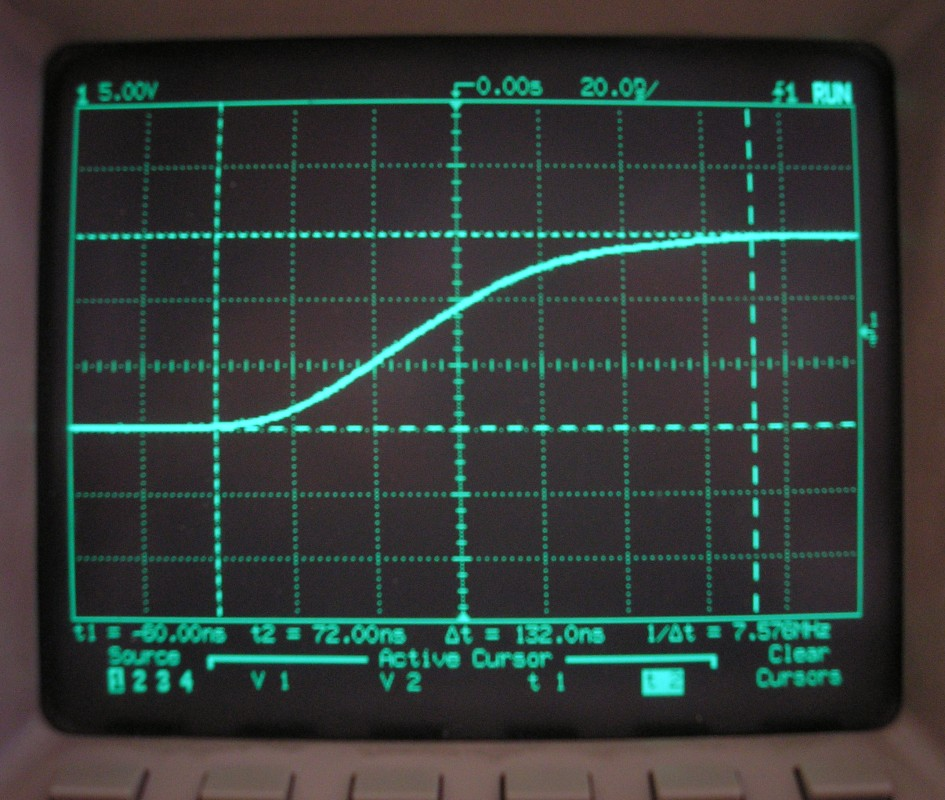
\includegraphics[height=8.4cm]{signaalit_pics/Digital_oscilloscope.jpg}\\
\tiny \url{http://commons.wikimedia.org/wiki/File:Digital\_oscilloscope.jpg}
\end{center}
}

\frame{
\begin{center}
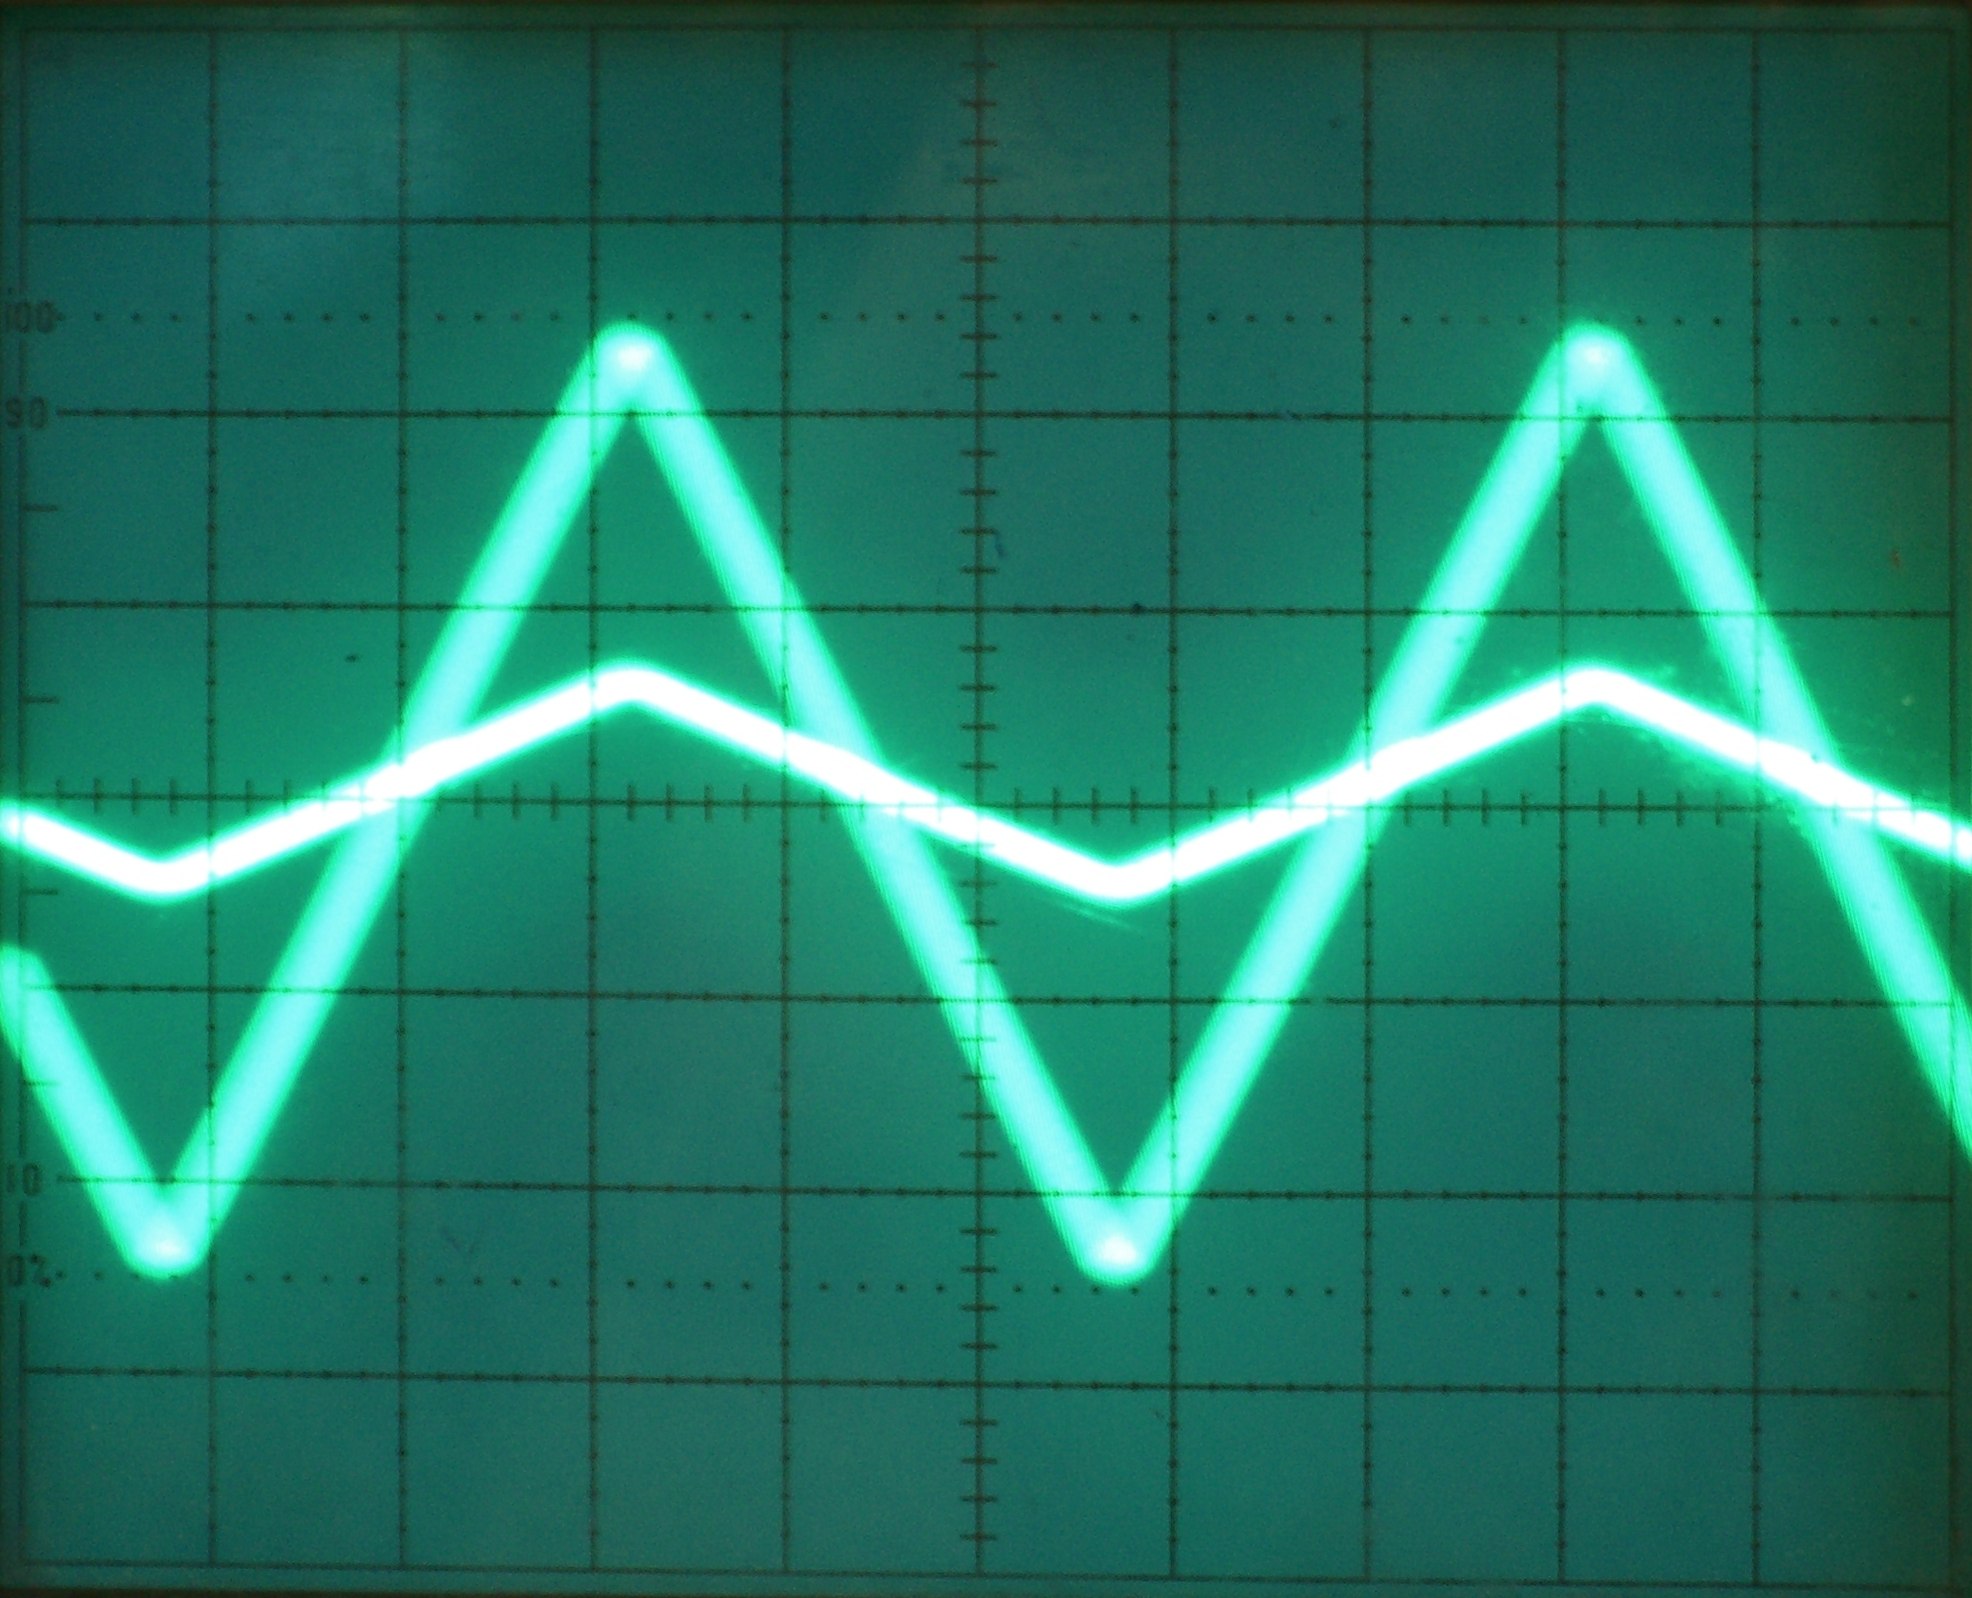
\includegraphics[height=8.4cm]{signaalit_pics/Oscilloscope_Triangle_Wave.jpg}\\
\tiny \url{http://commons.wikimedia.org/wiki/File:Oscilloscope\_Triangle\_Wave.jpg}
\end{center}
}

\frame{
\begin{center}
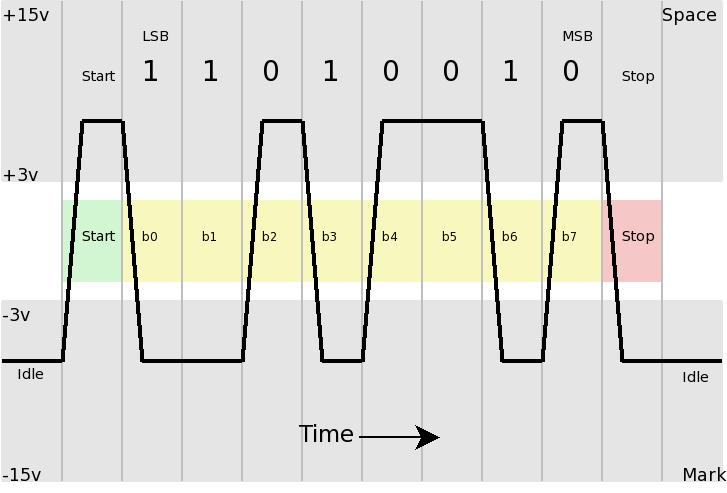
\includegraphics[height=8.1cm]{signaalit_pics/Rs232_oscilloscope_trace.jpg}\\
\tiny \url{http://commons.wikimedia.org/wiki/File:Rs232\_oscilloscope\_trace.jpg}
\end{center}
}

\frame{
\frametitle{Fourier'n teoreema}
Mikä tahansa jaksollinen signaali voidaan hajottaa siniaaltojen summaksi, valitsemalla
siniaalloille sopivat amplitudit, taajuudet ja vaihe-erot. Tätä summaa kutsutaan Fourier-sarjaksi.
Sähköisen signaalin Fourier-sarja muodostuu tasajännitekomponentista, perustaajuudesta ja perustaajuuden
monikerroista.

Hyvä esimerkki:\\
\url{http://commons.wikimedia.org/wiki/File:Fourier\_synthesis\_square\_wave\_animated.gif}

}


\frame{
\begin{center}
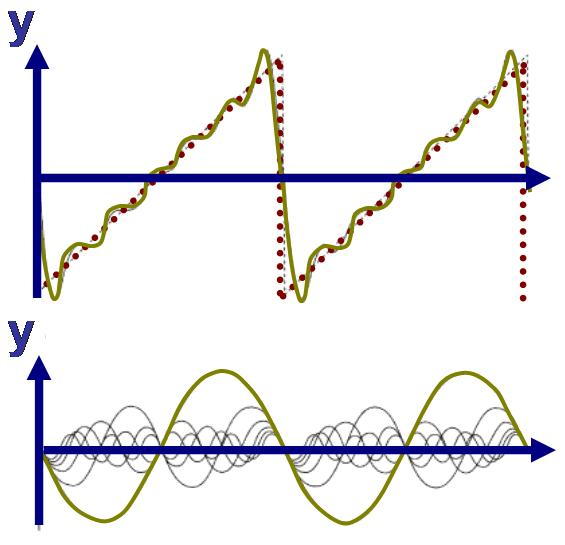
\includegraphics[height=8.4cm]{signaalit_pics/Sawtooth_Fourier_Analysis.JPG}\\
\tiny \url{http://commons.wikimedia.org/wiki/File:Sawtooth\_Fourier\_Analysis.JPG}
\end{center}
}

\frame{
\frametitle{Digitaalinen vs. analoginen}
\begin{itemize}
\item Analoginen signaali: signaali voi saada mitä tahansa arvoja, ja muuttua miten tahansa
ajan funktiona.
\item Digitaalinen signaali: signaalilla on määrätyt vakioarvot, ja se muuttuu ennalta sovitulla
tavalla (esim. 1000 000 kertaa sekunnissa).
\item Yleisesti käytössä oleva digitaalitekniikka käyttää binäärilogiikkaa, eli signaalilla on
kaksi sallittua tilaa, 0 ja 1.
\end{itemize}
}

\frame{
\frametitle{Digitaalinen vs. analoginen} % http://en.wikipedia.org/wiki/Analog_recording_vs._digital_recording
\begin{itemize}
\item Kun vertaat digitaalisia ja analogisia järjestelmiä, mitä eroja sinulle tulee mieleen?
\item Vinyyli vs. cd-levy? Analoginen televisio vs. digitelevisio?
\end{itemize}
}


\frame{
\frametitle{Signaalityypit}
Signaalit voidaan jakaa karkeasti analogisiin ja digitaalisiin signaaleihin. Tarkempi jako voidaan suorittaa jatkuva- ja diskreettiamplitudisiin sekä jatkuva- ja diskreettiaikaisiin signaaleihin. Esimerkkejä:
\begin{itemize}
\item Audiosignaali (vaikkapa mikrofonin tai kaiuttimen kaapelista mitattuna) on sekä jatkuva-aikainen että jatkuva-amplitudinen.

\item Ikkunannostimen rajakytkimeltä saatava signaali on diskreettiamplitudinen: sillä on kaksi tilaa, auki ja kiinni. Sen sijaan signaali on jatkuva-aikainen.

\item CD-levylle tallennettu musiikki on signaalina sekä diskreettiamplitudinen että diskreettiaikainen. Se on muodostettu audiosignaalista kvantisoimalla ja näytteistämällä.

\item Diskreettiaikaisesta mutta jatkuvasta signaalista on hankalampi keksiä jokapäiväistä esimerkkiä.
\end{itemize}
}



\frame{
\frametitle{Kvantisointi ja näytteistys}
\begin{block}{Kvantisointi}
Jatkuva-amplitudinen signaali muutetaan diskreettiamplitudiseksi kvantisoimalla. Mitä tarkemmin signaali halutaan tallentaa, sitä enemmän näytteistystasoja tarvitaan. Esimerkiksi cd-levyllä yksi ääninäyte tallennetaan 16 bitillä, eli mahdollisia tasoja on $2^{16}=65 536$.
\end{block}
\begin{block}{Näytteistys}
Jatkuva-aikainen signaali muutetaan diskreettiaikaiseksi näytteistämällä. Mitä suurempi taajuusalue halutaan tallentaa, sitä suurempi pitää näytteenottotaajuuden olla. Esimerkiksi cd-levyllä näytteenottotaajuus on 44,1 kHz, eli äänisignaalista tallennetaan näyte 44100 kertaa sekunnissa.
\end{block}
}

\frame{
\frametitle{Nyquistin näytteenottoteoreema}
Nyquistin näytteenottoteoreeman mukaan näytteenottotaajuuden on oltava vähintään kaksinkertainen verrattuna suurimpaan signaalitaajuuteen.

Esimerkiksi jos haluamme tallentaa ääntä taajuusalueella 0 Hz -- 20\,000 Hz, näytteenottotaajuuden on oltava
vähintään 40\,000 kHz.
}

\frame{
\frametitle{Laskostuminen}
Jos näytteenottotaajuus on $f_{\rm s}$, niin voimme tallentaa signaalit aina taajuuteen $f_{\rm s}/2$ asti. Taajuudet, jotka ovat suurempia kuin $f_{\rm s}/2$, on
suodatettava pois ennen näytteistystä, muuten ne siirtyvät haittasignaaliksi varsinaiselle taajuusalueelle eli {\em laskostuvat}. Esimerkiksi taajuudella $2f_{\rm s}+10\ Hz$ esiintyvä haittasignaali siirtyy hyötykaistalle taajuudelle 10 Hz.
\begin{center}
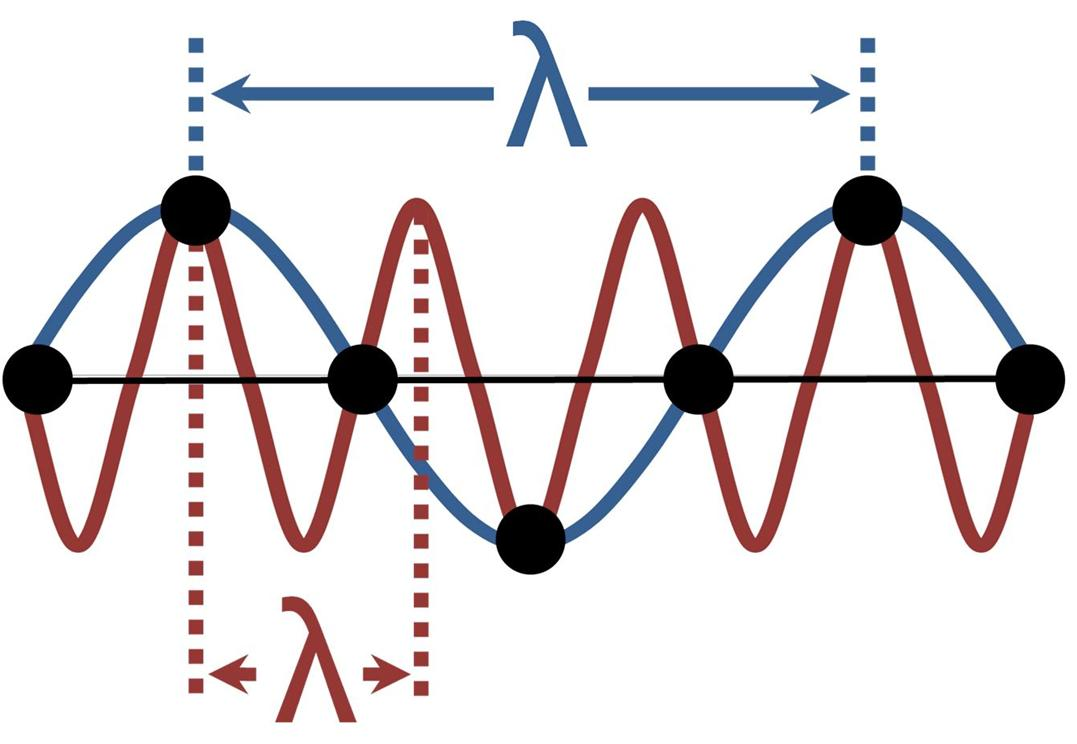
\includegraphics[height=4cm]{signaalit_pics/Wavelength_indeterminacy.JPG}\\
\tiny \url{http://commons.wikimedia.org/wiki/File:Wavelength\_indeterminacy.JPG}
\end{center}
}




\frame{
\frametitle{Kohina}
Kohina = hyötysignaalia häiritsevä satunnaisesti vaihteleva häiriö. Sähkölaitteissa kohinan lähteitä ovat
muun muassa
\begin{description}
\item[Taustakohina] Avaruudesta säteilynä välittyvä taustakohina.
\item[Lämpökohina] Varauksenkuljettajien lämpöliikkeestä aiheutuva kohina.
\item[$1/f$-kohina] Aiheutuu mm. puolijohteiden rajapintailmiöistä.
\item[Kvantisointikohina] eli kvantisointivirhe aiheutuu muunnettaessa analoginen signaali
digitaaliseksi.

\end{description}

}

\begin{frame}[fragile]

\frametitle{MATLAB-demo}
\small
\begin{verbatim}
x=linspace(0,1,20000); % 0..1 sekuntia, 20000 näytettä
y=sin(2*pi*1000*x);soundsc(y,20000); % 1000 Hz sinipiippaus
% molli:
y=sin(2*pi*440*x)+sin(2*pi*1.2*440*x)+sin(2*pi*1.5*440*x); 
% duuri:
y=sin(2*pi*440*x)+sin(2*pi*1.25*440*x)+sin(2*pi*1.5*440*x);
% Laskostuminen:
y=sin(2*pi*21000*x);soundsc(y,20000); 
% Kohina:
y=sin(2*pi*1000*x)+0.01*randn(size(x));soundsc(y,20000);
\end{verbatim}
\end{frame}

\frame{
\frametitle{Vahvistimet}
\begin{block}{Vahvistin} % Määritelmä Silvonen sivu 395
= elektroninen piiri, jolla signaalilähteestä tuleva signaali vahvistetaan, ja kytketään kuormaan tai ketjun seuraavalle laitteelle.
\end{block}
}

\frame{
\frametitle{Lineaarinen vahvistin}
\begin{center}
\begin{picture}(150,50)(0,0)
\cn{0,0}
\cn{0,50}
\hln{0,0}{50}
\hln{0,50}{50}
\vz{50,0}{R_{\rm in}}

\du{65,0}{u_{\rm in}}
\vst{150,0}{Au_{\rm in}}
\hln{150,0}{50}
\hz{150,50}{R_{\rm out}}
\cn{200,0}
\cn{200,50}
\end{picture}
\end{center}
}

\frame{
\frametitle{Vahvistimen toteuttaminen}
Halutunlainen vahvistin voidaan rakentaa esimerkiksi
\begin{itemize}
\item Operaatiovahvistimen avulla
\item Käyttämällä erilliskomponentteja, kuten bipolaaritransistoria tai MOSFET-transistoria
\end{itemize}
}
% TODO: siivoa vähän ja mieti järkevä paikka demotiedostolle

\frame{
\frametitle{MATLAB-harjoitukset}
MATLAB = MATrix LABoratory. Laajasti käytössä oleva numeerisen laskennan työkaluohjelmisto.
\begin{itemize}
\item Ohjelmalla suoritetaan laskutoimituksia skalaareille, vektoreille ja matriiseille.
\item Erittäin laaja valikoima valmiita funktioita.
\end{itemize}
Harjoitukset suoritetaan vapaamuotoisesti. Kokeile annettuja komentoja, kokeile omia komentoja. Pyri ymmärtämään, mitä kukin komento tekee!\\[1cm]
\scriptsize
Linux-käyttäjien on helppo kokeilla komentoja kotona vapaan Octave-ohjelmiston kanssa. Esim. Ubuntu 10.04:ssa: asenna paketit octave3.2, octave-audio ja octave-signal. Lisäksi pitää luoda kotihakemistoon tiedosto .octaverc ja luoda sinne rivi\\
global sound\_play\_utility = 'aplay';\\
jotta soundsc-funktio toistaa äänet.
}




\begin{frame}[fragile]
Tutki, mitä tapahtuu seuraavilla komennoilla:
\frametitle{MATLAB-harjoitukset}
\small
\begin{verbatim}
1+1
x=3
y=9
x+y
\end{verbatim}
Mitä eroa on seuraavilla kahdella komennolla
\begin{verbatim}
z=x+y
z=x+y;
\end{verbatim}
\end{frame}


\begin{frame}[fragile]
Vektorilaskutoimitukset
\frametitle{MATLAB-harjoitukset}
\small
\begin{verbatim}
x=[1,2,3]
2*x
x.^2
y=[3 4 5]
x.*y
\end{verbatim}
\end{frame}


\begin{frame}[fragile]
Käyrien piirtely
\frametitle{MATLAB-harjoitukset}
\small
\begin{verbatim}
x=linspace(0,100);
y=2*x
help plot
plot(x,y)
f=4
x=linspace(0,1,101);
y=2*sin(2*pi*f*sin(x));
plot(x,y)
\end{verbatim}
\end{frame}

\begin{frame}[fragile]
\frametitle{MATLAB-harjoitukset}
\small Lataa tiedosto \url{http://users.metropolia.fi/~vesali/aani.dat} ja tallenna se esim. työpöydälle.
Valitse MATLABin työhakemistoksi (vasemmasta ylänurkasta "Current folder") sama kansio, johon
tallensit tiedoston.
\begin{verbatim}
[y,Fs]=wavread('aani.dat'');
%typistetään vähän äänitiedostoa
z=y(1:308700);
soundsc(z)
%Mitä kyseinen äänitiedosto sisältää?
Kokeillaanpa uudestaan:
soundsc(z,Fs)
clear playsnd % Keskeyttää äänentoiston, jos tarvis
%ja pelleillään
soundsc(z,3*Fs)
soundsc(fliplr(z),Fs)
\end{verbatim}
\end{frame}




\begin{frame}[fragile]
\frametitle{MATLAB-harjoitukset}
Häiriön lisääminen
\small
\begin{verbatim}
N=length(z) % Tallennetaan näytemäärä
x=linspace(0,7,N);
h=0.1*sin(2*pi*1000*x);
e=h+z;
soundsc(e,Fs)
%wavwrite(e,Fs,'output.wav'); % Tällä voisi tallentaa tiedoston.
\end{verbatim}
\end{frame}

\begin{frame}[fragile]
\frametitle{MATLAB-harjoitukset}
\small
\begin{verbatim}
E=fft(e)/N; % Fourier-muunnos täytyy skaalata jakamalla näytemäärällä
plot(abs(E))
% Häiriöpiikin korkeus on puolet häiriön amplitudista. Syynä on se, että
% Matlabin Fourier-muunnosfunktio tekee muunnoksen kaksipuoleiseen
% taajuusalueeseen. Oikean korkuisena häiriö (ja muu signaali) näkyy
% komennolla
plot(2*abs(E))
% Piirroksessa on vaaka-akselina näytteiden määrä N. Kuinka saada näkymään
% häiriöpiikki oikealla taajuudella?
% Fourier-muunnoksessa taajuuden askellusväli (=kuinka suurta taajuutta
% vastaa yksi pykälä vaaka-akselilla):
f_step = Fs/N;
f = [0:f_step:(N-1)*f_step];
plot(f,2*abs(E))
\end{verbatim}
\end{frame}

\begin{frame}[fragile]
\frametitle{MATLAB-harjoitukset}
Fourier-käänteismuunnoksen voi kuunnella:
\small
\begin{verbatim}
soundsc(ifft(E),Fs)
\end{verbatim}
Tehtävä: poista häiriösignaali taajuustason esityksestä (Fourier-muunnetusta signaalista E). Vihje: komennosta \verb+find+
saattaa olla apua. Häiriö näkyy (kahtena) korkeana piikkinä taajuusspektrissä. Poista piikit.
\end{frame}


\begin{frame}[fragile]
\frametitle{MATLAB-harjoitukset}
Signaalin suodattaminen. Kokeile erilaisia suodattimia!
\small
\begin{verbatim}
[b,a]=butter(5,[600/22050,1000/22050]);
suod=filtfilt(b,a,z);
soundsc(suod,Fs)
help butter
\end{verbatim}
\end{frame}


% TODO?: Täällä on pari duplikaattikalvoa, desibelit ja johtimen magneettikenttä...
% TODO?: ... jääköön, ettei riko eheää kokonaisuutta.
\frame{
\frametitle{EMC = Electromagnetic compatibility}
\begin{itemize}
\item EMC = Sähkömagneettinen yhteensopivuus.
\item Sähkö- ja elektroniikkalaitteet on suunniteltava niin, että ne eivät {\bf häiritse} ympäristöä eivätkä {\bf häiriinny} ympäristön tavanomaisista häiriöistä.
\end{itemize}

}

\frame{
\frametitle{Käytännön esimerkkejä}
\begin{itemize}
\item Oletteko kohdanneet käytännön elämässä tilanteita sähkömagneettisesta yhteensopimattomuudesta?
\end{itemize}
}

\frame{
\frametitle{Käytännön esimerkkejä}
\begin{itemize}
\item GSM-puhelimen "laulu".
\item Radion rätinä kun naapuri poraa taulun seinään.
\item Radio napsuu kun loistelamput syttyvät.
\item Autonkeskuslukitus ja sähkökatto reagoivat kännykkään.
\item Sähköpyörätuoli koukkasi laiturilta veteen kun poliisiveneessä painettiin radiopuhelimen tangenttia.
\item Pietsosytkäri avaa pysäköintialueen puomin.
\item Hitsausmuuntajan päällekytkentä naapurirakennuksessa kaatoi telakan keskustietokoneen.
\end{itemize}
}

\frame{
\frametitle{Häiriölähteet} % EMC ja rakennusten sähkötekniikka s. 33
Häiriölähteet voidaan jakaa
\begin{itemize}
\item Luonnollisiin häiriöihin: salamointi ja kosminen taustasäteily.
\item Teknisiin häiriöihin: staattinen sähkö, digitaalipiirit, sähköverkon muutokset ja langaton viestintä.
\end{itemize}
}

\frame{
\frametitle{Häiriöiden kytkeytymistavat}
\begin{itemize}
\item Kytkeytyminen johtumalla
\item Kapasitiivinen kytkeytyminen (sähkökentän kautta)
\item Induktiivinen kytkeytyminen (magneettikentän kautta)
\item Sähkömagneettinen säteily
\end{itemize}
}



\frame{
\frametitle{Säännökset}
Jokaisen markkinoilla olevan sähkölaitteen on täytettävä sähköturvallisuus- ja EMC-määräykset.
\begin{itemize}
\item EMC-direktiivi 2004/108/EY
\item Radio- ja telepäätelaitteilla oma direktiivinsä 1999/5/EC
\item Ajoneuvoja koskee EMC-direktiivi 2004/104/EC.
\item Sähköturvallisuuslaki
\item Laki radiotaajuuksista ja telelaitteista
\item Standardit
\end{itemize}
}

\frame{
\frametitle{EMC-direktiivi}
\ldots lähestymistavan mukaan laitteiston suunnittelussa ja valmistuksessa on noudatettava sähkömagneettista yhteensopivuutta koskevia olennaisia vaatimuksia. Nämä vaatimukset ilmaistaan yhdenmukaistettuina eurooppalaisina standardeina, jotka useat eurooppalaiset standardointielimet, Euroopan standardointikomitea (CEN), Euroopan sähkötekniikan standardointikomitea (CENELEC) ja Euroopan telealan standardointilaitos (ETSI) hyväksyvät. CEN, CENELEC ja ETSI ovat toimivaltaisia hyväksymään tämän direktiivin soveltamisalaan kuuluvat yhdenmukaistetut standardit, jotka ne laativat niiden ja komission välisestä yhteistyöstä annettujen yleisten suuntaviivojen sekä teknisiä standardeja ja määräyksiä\ldots
}

\frame{
\frametitle{Sähköturvallisuuslaki}
Sähkölaitteet ja -laitteistot on suunniteltava, rakennettava, valmistettava ja korjattava niin sekä niitä on huollettava ja käytettävä niin, että:

1) niistä ei aiheudu kenenkään hengelle, terveydelle tai omaisuudelle vaaraa;

2) niistä ei sähköisesti tai sähkömagneettisesti aiheudu kohtuutonta häiriötä; sekä

3) niiden toiminta ei häiriinny helposti sähköisesti tai sähkömagneettisesti.
}

\frame{
\frametitle{Standardit}
\begin{itemize}
\item Monelle laitetyypille on oma standardinsa. Yleisstandardia sovelletaan, mikäli laitekohtaista ei ole olemassa.
\end{itemize}

\url{http://www.tukes.fi/fi/Toimialat/Sahko-ja-hissit/EMC/}

}

\frame{
\frametitle{Häiriötestit}
\begin{itemize}
\item Häiriöpäästöt: Radiotaajuiset päästöt ja pientaajuuspäästöt.
\item Häiriönsieto: ESD, Radiotaajuinen sm-kenttä, nopeat kytkentätransientit ("jännitepiikit"), syöksyaalto, radiotaajuinen jännite, harmoniset taajuudet,
magneettikenttä, pulssimuotoinen magneettikenttä, jännitekatkokset, \ldots
\end{itemize}
}

\frame{
\frametitle{Viranomaisvalvonta}
Laitteita ei tarkasteta erikseen viranomaisten toimesta, vaan testaus on valmistajan vastuulla.
Turvatekniikan keskus (Tukes) voi määrätä myyntikieltoon EMC-säännöksiä rikkovan laitteen.

\url{http://marek.tukes.fi/}

}

\frame{
\frametitle{Häiriöiden torjunta}
\begin{itemize}
\item Häiriön synnyn estäminen
\item Etenemisen katkaiseminen
\item Sietokyvyn parantaminen
\end{itemize}
}

\frame{
\frametitle{Häiriöiden torjunta}
\begin{itemize}
\item Johtimien järjestely
\item Symmetrointi
\item Suodatus
\item Digitaalitekniikan käyttö
\item Valokaapelin käyttö
\end{itemize}
}


\frame{
\frametitle{Fysikaalista taustaa}
\begin{itemize}
\item Sähkövirta ja/tai muuttuva sähkökenttä saa aikaan magneettikentän.
\item Muuttuva magneettikenttä indusoi johtimeen jännitteen.
\item Sähkövaraus aikaansaa sähkökentän.
\end{itemize}
}




\frame{
\frametitle{Coulombin laki ja sähkökenttä}
Samanmerkkiset sähkövaraukset hylkivät toisiaan ja erimerkkiset vetävät toisiaan puoleensa voimalla
\[
F=k\frac{|q_1q_2|}{r^2}\qquad k=\frac{1}{4\pi \epsilon_0}
\]
Sähkökenttä määritellään testivarauksen avulla. Mitä suurempi voima testivaraukseen vaikuttaa, sitä voimakkaampi
on sähkökenttä.
\[
\vec{E}=\frac{\vec{F}}{q}
\]
Kentänvoimakkuuden $E$ yksikkö on $\rm \frac{N}{C}$ tai tavallisemmin $\rm \frac{V}{m}$.
}

\frame{
\frametitle{Magneettikentän voimakkuus}
\begin{itemize}
\item Suorassa johtimessa kulkeva sähkövirta $I$ aiheuttaa johtimen ympärille magneettikentän.
\item Magneettikentän voimakkuus etäisyydellä $r$ on $H=\frac{I}{2\pi r}$. Yksikkö on $\rm \frac{A}{m}$.
\item Yleisemmin: nopeudella $v$ liikkuva varaus aikaansaa magneettikentän
\[
\vec{B}=\frac{\mu_0}{4\pi}\int \frac{q\vec{v}\times \hat{r}}{r^2}
\]
\end{itemize}
}

\frame{
\frametitle{Magneettivuo}
\begin{itemize}
\item Magneettivuon tiheys $B$ riippuu magneettikentän voimakkuudesta $H$ ja väliaineen permeabiliteetista $\mu$
\[
B=\mu H
\]
\item Vuontiheyden yksikkö on tesla (T). Puhekielessä magneettikentän voimakkuus ja magneettivuon tiheys menevät usein sekaisin (esim. mitataan vuontiheyttä ja puhutaan kentänvoimakkuudesta).
\item Pinta-alan $A$ läpi kulkeva magneettivuo $\phi$ on
\[
\phi = \int_A \vec{B}\cdot {\rm d} \vec{A}
\]
\end{itemize}
}


\frame{
\frametitle{Sähkömagneettinen induktio}
\begin{itemize}
\item Faradayn lain mukaan muuttuva magneettivuo $\phi$ indusoi käämiin jännitteen, jonka suuruus on
\[
e=-\frac{{\rm d}\phi }{{\rm d}t}
\]
\end{itemize}
}


\frame{
\frametitle{Kapasitiivisten häiriöiden torjunta}
\begin{itemize}
\item Metallikotelointi
\item Johtimien välisen etäisyyden ja suunnan muuttaminen
\item Johtimien sijoittelu lähelle maatasoa
\item Impedanssitason pienentäminen
\end{itemize}
}

\frame{
\frametitle{Induktiivisten häiriöiden torjunta}
\begin{itemize}
\item Johtimien sijoittelu
\item Impedanssitason pienentäminen
\end{itemize}
}

\frame{
\frametitle{Impedanssitason pienentäminen}
\begin{itemize}
\item Impedanssitason pienentämisellä on välitön vaikutus vastaanotettujen häiriöiden voimakkuuteen.
\end{itemize}
}


\frame{
\frametitle{Sähkömagneettinen yhteensopivuus ei ole erillinen asia}
Laitetta ei voi suunnitella niin, että ensin suunnitellaan laite je sitten lopuksi ihmetellään, miten se saadaan sähkömagneettisesti yhteensopivaksi.
{\bf EMC pitää ottaa huomioon koko suunnitteluprosessin ajan.}
}


\frame{
\frametitle{Häiröiden lähteet ja niiden kytkeytyminen}
\begin{itemize}
\item Häiriölähteiden mallintaminen on yleensä monimutkaista käsiteltäväksi matemaattisesti.
\item Edellyttää Maxwellin yhtälöiden ratkaisemista.
\item Usein pärjätään likimääräisillä kaavoilla tai pelkästään kvalitatiivisella käsittelyllä.
\end{itemize}
}

\frame{
\frametitle{Kapasitiivisesti kytkeytyvän häiriön mallitaminen}
\begin{itemize}
\item Kapasitiivinen kytkeytyminen eli sähkökentän kautta kytkeytyminen voidaan mallintaa kondensaattorilla.
\item $\epsilon = \epsilon_o\epsilon_r$
\item Levykondensaattorin kapasitanssi
\[
C=\epsilon \frac{A}{d}
\]
\item Kahden yhdensuuntaisen johtimen välinen kapasitanssi
\[
C\approx \frac{\pi \epsilon l}{\ln \frac{d}{\sqrt{r_1r_2}}}
\]
missä $l$ on johtimen pituus, $r$ johtimen säde ja $d$ johtimien välinen etäisyys. Kaava on likimääräinen ja toimii
vain, kun $d>> r_1r_2$.

\end{itemize}
}

\frame{
\frametitle{Kapasitiivisesti kytkeytyvän häiriön mallitaminen}
\begin{itemize}
\item Johtimen ja sen kanssa yhdensuuntaisen tason välinen kapasitanssi on
\[
C=\frac{2\pi\epsilon l}{\ln \frac{d+\sqrt{d^2-r^2}}{r}}
\]
missä $d$ on johtimen keskiakselin etäisyys tasosta.
\end{itemize}
}

\frame{
\frametitle{Esimerkkejä}
\begin{itemize}
\item Hakkuriteholähteen toimintataajuus on 100 kHz ja virtajohtimesta noin 10 cm pätkä kulkee aivan laitteen kotelon pintaa pitkin. Johtimen säde on 2 mm ja eristeen
paksuus on 1 mm. Kuinka suuri on kyseinen hajakapasitanssi ja kuinka suuri virta sen läpi kulkee, jos johtimessa oleva 100 kHz:n hurinajännite on amplitudiltaan
50 millivolttia?
\item Kuinka suuren magneettivuon tiheyden johdin aiheuttaa 10 cm etäisyydelle (oletetaan, että johdin on pitkä ts. käytetään yksinkertaista kaavaa)?
\item Jos johtimessa kulkee 50 ampeerin virta ja se katkaistaan yhtäkkiä (5 millisekunnissa), kuinka suuren jännitteen se indusoi 10 senttimetrin etäisyydellä olevaan
silmukkaan, joka on kohtisuorassa vuota vastaan ja jonka pinta-ala on 10 cm$^2$.
\item Oletetaan molemmissa tapauksissa väliaineen materiaaliksi tyhjiö ($\epsilon_0\approx 8,854\cdot 10^{-12} \rm \frac{F}{m}$ ja $\mu_0\approx 1,26\cdot 10^{-6}\rm \frac{H}{m}$ ).
\end{itemize}
}

\frame{
\frametitle{Verkkosuodatin ja vuotovirta maahan}
\begin{itemize}
\item Jos tietokoneen liittää maadoittamattomaan pistorasiaan, sen rungosta voi saada vaimean sähköiskun.
\item Tämä johtuu verkkosuodattimen kondensaattoreista.
\item Verkkosuodattimen tarkoitus on estää hakkuriteholähteen ja digitaalipiirien häiriöjännitteiden karkaaminen sähköverkkoon.
\item Suodatin rakentuu differentiaalisesta kelasta sekä kondensaattoreista. Joskus käytetään myös VDR-vastuksia.
\item Vuotovirta saa olla enintään 0,5 milliampeeria (EN 60601-1-1).
\end{itemize}
}

\frame{
\frametitle{Yhteismuotoinen häiriö ja eromuotoinen häiriö} % EMC-kirja s. 323
Ajatellaan kahta piiriä, jotka on kytketty toisiinsa kaksinapaisella kaapelilla.
\begin{itemize}
\item Eromuotoinen jännite tarkoittaa johtimien välistä jännitettä ja eromuotoinen virta tarkoittaa johtimissa eri suuntiin kulkevia mutta yhtä suuria virtoja.
\item Yhteismuotoinen jännite tarkoittaa johtimien ja maatason välistä jännitettä ja yhteismuotoinen virta johtimissa yhteen suuntaan kulkevaa virtaa.
\end{itemize}
Yhteismuotoinen kytkentä aikaansaa yhden suuren silmukan piirien välille yhdessä maatason kanssa.
}

\frame{
\frametitle{Komponenttien jännitteenkesto}
Verkkosuodattimen komponenttien tulee täyttää standardin EN132400 mukaiset jännitteenkesto- ja paloturvallisuusvaatimukset.
\begin{itemize}
\item Kondensaattorien tulee kestää 2,5 kilovoltin 50 $\mu$s pulsseja. 
\item Kondensaattorien tulee suoriutua 1000 tunnin kestotestistä 1,25-kertaisella nimellisjännitteellä siten, että tunnin välein niitä häiritään 1 kV vaihtosähköpiikillä.
\end{itemize}
}

% Layout and grounding, kappale 11 EMC for product designers

\frame{
\frametitle{EMC ja tuotesuunnittelu}
\begin{itemize}
\item Häiriöiden lähetys ja vastaanotto tulee pitää mielessä koko suunnitteluprosessin ajan.
\item Komponenttien asettelu on tärkeä osa EMC-suunnittelua.
\end{itemize}
}

\frame{
\frametitle{Kolmitasoinen suojaus}
\begin{itemize}
\item Piirilevyn asettelu
\item Rajapintojen suodattimet
\item Suojakotelo
\end{itemize}
}

\frame{
\frametitle{Suojauksen tarve}
\begin{itemize}
\item Ei-kriittisissä sovelluksissa pärjätään usein pelkällä piirilevyn asettelun huomioon ottamisella.
\item Näin on varsinkin, jos laitetta ei liitetä muualla kaapeleilla. Esimerkki: television kauko-ohjain.
\item Laitteen suojaaminen metallivaipalla on valmistusteknisesti kallista.
\end{itemize}
}

\frame{
\frametitle{Komponenttien asettelu piirilevylle}
\begin{itemize}
\item 90 prosenttia suunnittelun jälkeisistä EMC-ongelmista johtuu huonosta piirilevysuunnittelusta.
\end{itemize}
}

\frame{
\frametitle{Tärkeimmät suunnitteluperiaatteet}
\begin{itemize}
\item Jaa järjestelmä osiin.
\item Ajattele maata virran kulkualueena.
\item Maadoituksella voi estää häiriövirtojen pääsyn signaalipiireihin. Valitse maadoituspisteet huolella ja minimoi maadoitusimpedanssi.
\item Muista mekaniikkasuunnittelua tehdessäsi, että jokainen johtava osa voi kuljettaa häiriövirtoja.
\end{itemize}
}

\frame{
\frametitle{Järjestelmän osiointi}
\begin{itemize}
\item Jaa piirit kriittisiin ja ei-kriittisiin osiin.
\item Piirit, jotka eivät häiriinny eivätkä häiritse helposti, sijoitetaan omiin piirilevyn osiin tai kokonaan eri piirilevyille.
\item Häiriöherkkyyteen vaikuttavat mm. signaalitasot, kaistanleveydet ja tietenkin piirin tarkoitus ja toiminta.
\item Esimerkiksi lineaariset teholähteet, ilman kellopulssia toimivat logiikkapiirit ja tehovahvistimet eivät juuri häiriinny eivätkä häiritse.
\end{itemize}
}

\frame{
\frametitle{Maadoittaminen}
\begin{block}{Helsingin Sanomat 22.8.2005: Georgiasta löydetty 1,8 miljoonaa vanha pääkallo }
Arkeologit uskovat löytäneensä Georgiasta maadoittamattoman pääkallon, jota epäillään 1,8 miljoonaa vuotta vanhaksi. \ldots
\end{block}
\begin{itemize}
\item Earthing, suojamaadoitus. Laitteen rungon kytkeminen sähköverkon maapotentiaaliin.
\item Grounding, maadoitus. Kytketään piirielementtejä samaan yhteiseen referenssipotentiaaliin.
\end{itemize}
Koska maataso ei ole ideaalinen, potentiaali vaihtelee maatason sisällä. Ks. esimerkki (Williams, s. 262).
}

\frame{
\frametitle{Toinen kevennys}
\begin{block}{Helsingin Sanomat 11.4.1990}
"Tuoreen norjalaistutkimuksen mukaan matkapuhelimen antennista säteilee lähetysvaiheessa sähkömagneettisia aaltoja."
\end{block}
No shit, Sherlock!
}

\frame{
\frametitle{Maadoitustapoja}
\begin{itemize}
\item Yksipistemaadoitus. Ehkäisee häiriöjännitteitä, jotka syntyvät yhteisten impedanssien läpi kulkevista virroista. Suurilla taajuuksilla maadoitusjohtimet käyttäytyvät kuin siirtojohdot, jolloin komponentit eivät ole enää samassa potentiaalissa.
\item Monipistemaadoitus. Toimii hyvin suurilla taajuuksilla. Jokaisella piirillä on oma maa, ja nämä maat yhdistetään toisiinsa lyhyillä johtimilla.
\end{itemize}
Yksipistemaadoitus on yleinen esimerkiksi hakkuriteholähteissä. Nyrkkisääntö: alle 1 MHz taajuuksilla yksipistemaadoitus, ja yli 10 MHz:n taajuuksilla monipistemaadoitus.
}

\frame{
\frametitle{Asettelu yksipuoleiselle piirilevylle}
\begin{itemize}
\item Piirilevyn johtimen sarjainduktanssi riippuu johtimen dimensioista. Esimerkiksi 0,5 mm levyisen 10 cm pituisen kupariliuskan
induktanssi on noin 60 nH. Kymmenien megahertsien taajuuksilla impedanssi on jo merkittävä.
\item Maadoitus tulee tapahtua ristikkomaisella liuskarakenteella. Kampamainen on huonoin mahdollinen (Williams s. 270).
\item Maatasoon ei saa jäädä isoja koloja (Williams s. 275).
\end{itemize}
}


\frame{
\frametitle{Maatason käyttö}
\begin{itemize}
\item Monikerrospiirilevyllä maadoitus on helppo toteuttaa käyttämällä laajaa maatasoa.
\item Nopeilla digitaalipiireillä ja radiotaajuuksilla maatason käyttö on käytännössä pakollista.
\item Maatason päätarkoitus on tarjota matala maadoitusimpedanssi. Toissijainen tarkoitus on suojata sähkökentiltä.
\end{itemize}
}

\frame{
\frametitle{Monikerrospiirilevyt}
\begin{itemize}
\item Massavalmistetussa elektroniikassa käytetään yleensä nelikerrospiirilevyä.
\item Yksi taso on maataso, toinen on käyttöjännitteen syöttötaso, johtimet ovat kahdella muulla tasolla.
\end{itemize}
}

\frame{
\frametitle{Ylikuuluminen}
\begin{itemize}
\item Kaksi vierekkäistä johdinta piirilevyllä on (valitettavasti) kytketty toisiinsa induktiivisesti ja kapasitiivisesti.
\item Toisen johtimen signaali voi "ylikuulua"\ (crosstalk) toiseen.
\item Käytännössä ylikuulumista ei esiinny, jos johtimet ovat yli 1 cm päässä toisistaan.
\item Maatason käyttö ja impedanssitason pudottaminen ehkäisevät ylikuulumista.
\end{itemize}
}

\frame{
\frametitle{Tehonsiirto ja jäähdytys}
\begin{itemize}
\item Suurtaajuuspiireissä käyttöjännitteiden syöttötasot tulee pilkkoa pieniin osiin, jotka kytketään toisiinsa RF-kuristimien välityksellä. Tarkoituksena on estää ilmiö, jossa maatason ja käyttöjännitetason muodostama voileipämäinen rakenne käyttäytyy antennina.
\item Mahdolliset jäähdytyselementit tulee maadoittaa useasta kohdasta. Eristetty jäähdytyselementti aiheuttaa ongelmia (s. 282).
\end{itemize}
}

\frame{
\frametitle{Tarkistuslista}
\begin{itemize}
\item Vältä pitkiä johtimia piirilevyllä.
\item Herkkiä ja häiritseviä komponentteja ei vierekkäin.
\item Herkkiä piirin osia ei sijoitella maatason reunoille.
\item Osioi piiri huolellisesti.
\end{itemize}
}


\frame{
\frametitle{Rajapinnat ja suodatus}
\begin{itemize}
\item Piirilevytason EMC-suunnittelun lisäksi on tärkeää ottaa huomioon kytkentärajapintojen käyttö.
\item Vain harva laite on sellainen, jota ei kytketä johtimilla mihinkään (kaukosäädin, taskulaskin).
\end{itemize}
}

\frame{
\frametitle{Ferriittikuristimet} % O'hara s. 31
\begin{itemize}
\item Yleisiä esimerkiksi datakaapeleissa.
\item Lisää sarjainduktanssin kaapeliin.
\item Vaimentaa taajuuksia suurin piirtein välillä 1--1000 MHz.
\item Haittapuolena on suhteellisen pieni vaimennus (enimmillään 10--20 dB). Hyvänä puolena on jälkiliitettävyys (komponentilla voidaan
paikata jälkikäteen suunnittelukömmähdyksiä).
\item Ferriittikuristin vaimentaa tehokkaasti myös ESD-purkausten aiheuttamia nopeita transienttipulsseja.
\end{itemize}
}

\frame{
\frametitle{Staattiselta sähköltä suojautuminen}
\begin{itemize}
\item Oletteko koskaan rikkoneet laitteita staattisella sähköllä?
\item Mitä varotoimia tarvitaan esimerkiksi tietokoneen näytönohjainta asennettaessa (tai muuta tietotekniikkahuoltoa tehtäessä).
\end{itemize}
}

\frame{
\frametitle{Staattiselta sähköltä suojautuminen} % O'hara s. 55
\begin{itemize}
\item JFET- ja erityisesti MOSFET-komponentit ovat herkkiä staattiselle sähkölle.
\item Hilakapasitanssi on pieni. Jos siihen tulee suuri sähkövaraus, jännite kipuaa satoihin voltteihin ja tapahtuu läpilyönti.
\item Suojaus diodeilla tai hilavastuksella.
\end{itemize}
}

\frame{
\frametitle{Jännitepiikeiltä suojautuminen}
\begin{itemize}
\item VDR-vastus.
\item Ylijännitesuoja (GDT, Gas Discharge Tube).
\item Kaasupurkausputket pystyvät käsitteleämään huomattavan suuria virtoja (kymmeniä kiloampeereja).
\end{itemize}
}

\frame{
\frametitle{Kaapelien suojaus} % O'hara s. 95- ja Williams s. 344
\begin{itemize}
\item Kaapeli voidaan suojata suojavaipalla.
\item Molemmista päistä maadoitettu vaippa suojaa hyvin magneettisilta häiriöiltä.
\item Toisesta päästä maadoitettu vaippa suojaa hyvin sähköisiltä häiriöiltä.
\end{itemize}
}

\frame{
\frametitle{Kierretty pari}
\begin{itemize}
\item Edullinen suojausratkaisu, toimii muutamaan megahertsiin asti.
\item Suojaamalla kaapeli suojavaipalla voidaan taajuuskaistaa laajentaa entisestään.
\item Suojavaippa tulee kiinnittää joka puolelta. "Porsaanhäntäkytkentä", jossa vaippa kiinnitetään runkoon yhdellä johtimella,
aiheuttaa sarjainduktanssin, joka käytännössä katkaisee maadoituksen suurilla taajuuksilla.
\end{itemize}
}

\frame{
\frametitle{Kytkinten suojaaminen} % O'hara s. 105
\begin{itemize}
\item Mekaaniset kytkimet aiheuttavat häiriöitä kahdella tavalla.
\item Toisiaan lähellä olevien kytkinliuskojen välille voi syttyä valokaari.
\item Kytkinliuskat koskevat toisiinsa monta kertaa ennen kuin sulkeutuvat ("bouncing").
\item Vaimennus kytkimen rinnalle asennettavalla RC-sarjapiirillä.
\end{itemize}
}

\frame{
\frametitle{Releet}
\begin{itemize}
\item Rele tuottaa häiriöitä sekä kosketinpuolella että solenoidissa.
\item Häiriöitä voidaan vaimentaa RC-vaimentimella tai suojadiodilla.
\item Suojadiodin käyttö on usein välttämätöntä relettä ohjaavan transistorin suojelemiseksi jännitepiikiltä.
\end{itemize}
}

\frame{
\frametitle{Moottorit}
\begin{itemize}
\item Sähkömoottorit ovat voimakkaita sähkömagneettisten häiriöiden lähteitä.
\item Moottori itsessään luo ympärilleen magneettikentän, ja virran katkeaminen ja kytkeminen sekä kipinöinti kommutaattorissa
aiheuttavat laajakaistaisia radiotaajuisia häiriöitä.
\item Moottorin metallirunko estää häiriöiden etenemistä, mutta usein on järkevää sijoittaa suojakondensaattorit moottorin napojen väliin
sekä kummankin navan ja maan väliin.
\end{itemize}
}


\frame{
\frametitle{Lainsäädäntö ja standardit}
\begin{itemize}
\item Sivuttu jo: kalvot 11-14.
\item Standardien ulkoa opetteleminen ei ole tarkoituksenmukaista. Esimerkiksi SFS-käsikirja 660, johon on koottu olennaisimmat standardit, sisältää yli 400 sivua.
\end{itemize}
}

\frame{
\frametitle{Standardien suhde lainsäädäntöön}
\begin{itemize}
\item EU:n EMC-direktiivin mukaisuus voidaan (ei ole pakko) osoittaa EN-standardeja käyttämällä.
\item Käytännössä vaatimustenmukaisuuden osoittaminen käyttämättä standardeja on niin monimutkaista, että standardien käyttö on käytännössä pakollista.
\end{itemize}
}

\frame{
\frametitle{Standardit}
\begin{itemize}
\item Perusstandardeissa määritellään EMC-testausmenetelmät ja testiympäristöjen vaatimukset.
\item Yleisstandardeissa määritellään tiettyihin toimintaympäristöihin tarkoitettujen laitteiden vaatimukset.
\item Tuote- ja tuoteperhestandardeissa määritellään nimensä mukaisesti jonkun tuotteen tai tuoteperheen tarkemmat EMC-vaatimukset. Jos tuotteella ei ole omaa standardia, käytetään yleisstandardeja.
\end{itemize}
}

\frame{
\frametitle{Standardien synty}
\begin{itemize}
\item IEC (International Electrotechnical Commission) on maailman suurin sähköalan standardointiorganisaatio.
\item Sen komiteoissa IEC/CISPR ja IEC/TC 77 laaditaan EMC-standardeja.
\item Kun eurooppalainen sähköalan standardointiorganisaatio CENELEC hyväksyy standardin, siitä tulee EN-standardi.
\item Suomessa standardit hyväksyy SESKO ja ne vahvistetaan edelleen SFS-EN-standardeiksi.
\end{itemize}
}

\frame{
\frametitle{Lähteitä}
\begin{itemize}
\item Standardien hankkiminen on yleensä kallista.
\item Suomessa neuvoa antava viranomainen on Tukes (Turvatekniikan keskus).
\item Kun aloittaa laitteen suunnittelun, voi Tukesilta kysyä tietoa ajantasaisista standardeista.
\item \url{http://www.edilex.fi/tukes/fi/}
\item \url{http://www.tukes.fi/fi/Toimialat/Sahko-ja-hissit/EMC/}
\item \url{http://www.ake.fi/AKE/Katsastus_ja_ajoneuvotekniikka/Tutkimuslaitokset+ja+hyväksytyt+asiantuntijat/}
\item Hyvä tiivistelmä: \url{http://www.sahkoautot.fi/wiki:saehkoeautojen-emc-hyvaeksynnaet}
\end{itemize}
}

\frame{
\frametitle{Ajoneuvot} % http://www.fi.sgs.com/sgssites/fimko/fi/ajoneuvoelektroniikan-testaukset.htm
\begin{itemize}
\item Ajoneuvojen EMC-direktiivi 2004/104/EC
\item EN 55012:2002 Ajoneuvot, veneet ja polttomoottorikäyttöiset laitteet — Radiohäiriöt — Raja-arvot
ja mittausmenetelmät radiovastaanoton suojaamiseksi lukuun ottamatta ajoneuvoon/
veneeseen/laitteeseen itseensä tai viereiseen ajoneuvoon/veneeseen/laitteeseen asennettuja
vastaanottimia
\item EN 14010:2003 Mm. moottoriajoneuvojen konekäyttöiset pysäköintilaitteistot.
\item Ajoneuvoon asennettava elektroniikka on testattava puolueettomassa laboratoriossa (esim. Nemko, SGS Fimko jne.).
\end{itemize}
}



\frame{
\frametitle{Tärkeitä standardeja}
\begin{itemize}
\item EN 61000-4-[3-4] Perusstandardit häiriöpäästöjen testaukselle.
\item EN 61000-6-[1-6] Perusstandardit häiriönsiedon testaukselle.
\item EN 55022 Tietoteknisten laitteiden tuoteperhestandardi häiriöpäästöille.
\item EN 55024  Tietoteknisten laitteiden tuoteperhestandardi häiriönsiedolle.
\item Ajoneuvoille on omat standardit (2004/104/EY).
\item Sotilas-, ilmailu-, ja rautatielaitteille omat standardit.
\end{itemize}
}

\frame{
\frametitle{Ajoneuvoelektroniikan standardit}
\begin{itemize}
\item Päästöille CISPR\footnote{Comité International Spécial des Perturbations Radioélectriques} 12 ja 25.
\item Siedolle ISO 7637, 11451 ja 11452.
\item Ks. Williams s. 102--103.
\end{itemize}
}

%\frame{
%\frametitle{Ajoneuvon testit}
%\begin{itemize}
%\item Ajoneuvoa ei liitetä johdoilla mihinkään, joten käytännössä sille suoritetaan ainoastaan sähkö- ja magneettikentänsietotesti joka suunnasta sekä mitataan sähkö- ja magneettikenttäpäästöt.
%\end{itemize}
%}


\frame{
\frametitle{EMC-päästömittaukset}
\begin{itemize}
\item Yksinkertaisia mittauksia voi tehdä spektrianalysaattorin avulla (hinnat useista tuhansista kymmeniin tuhansiin euroihin).
\item Erityisesti EMC-testeihin suunnitellut mittavastaanottimet maksavat kymmeniä tuhansia euroja.
\end{itemize}
}

\frame{
\frametitle{Miksi käyttää varta vasten suunniteltua EMC-mittavastaanotinta}
\begin{itemize}
\item Parempi herkkyys
\item Paremmat sisääntuloliitäntöjen suojaukset
\item Laitteen ominaisuudet on valmiiksi suunniteltu täyttämään standardien vaatimukset.
\end{itemize}
}

\frame{
\frametitle{Mitta-antennit}
\begin{itemize}
\item Suuri osa kaukokenttäpäästömittauksista tehdään 30MHz-1GHz alueella.
\item Mittaus onnistuu esimerkiksi kaksoiskartio- ja logperiodiantennien yhdistelmällä (BiLog).
\item Lähikentän mittaukseen (sähkö- ja magneettikenttä) käytetään sauva- ja silmukka-antennia.
\end{itemize}
}

\frame{
\frametitle{Magneettikentän mittaus silmukalla}
\begin{itemize}
\item Magneettikentän voimakkuus on helppo mitata silmukka-antennilla
\[
U=\mu_0 N A 2\pi f H
\]
\end{itemize}
}

\frame{
\frametitle{Sähkökentän mittaus sauva-antennilla}
\begin{itemize}
\item 1 metrin mittainen sauva-antenni mittaa pystysuoran sähkökentän voimakkuuden, käytetään mm. standardien CISPR 12 ja 25 mukaisissa testeissä. 
\end{itemize}
}

\frame{
\frametitle{Päästöjen paikallistaminen}
\begin{itemize}
\item Koaksiaalikaapelista on helppo askarrella lähikenttäantenni, jonka avulla voi etsiä piirin osan, josta jokin tietty häiriö on peräisin.
\item Ks. Williams s. 139
\end{itemize}
}

\frame{
\frametitle{Virhelähteet}
\begin{itemize}
\item Mittalaitteiden epätarkkuus.
\item Kaapelihäviöt.
\item Väärä impedanssisovitus.
\item Heijastukset seinistä.
\item Ulkopuoliset kentät.
\item Inhimilliset virheet.
\end{itemize}
}

\frame{
\frametitle{EMC-sietomittaukset}
\begin{itemize}
\item Moduloitava signaaligeneraattori
\item Tehovahvistin
\item Välineet kentänvoimakkuuden valvontaan
\item Radioaalloilta eristetty kaiuton huone
\item ESD-pulssigeneraattori
\end{itemize}
}

\frame{
\frametitle{Johtuvien häiriöiden sieto}
\begin{itemize}
\item Häiriöt syötetään kytkentäjohtoihin erityisen kytkentäverkon, virtamuuntajan tai ferriittipihdin avulla (EN 6100-4-6).
\item Sähköverkon häiriöiden mallintamiseen on omat mittageneraattorinsa (jännitekatkokset, jännitepiikit, harmoniset yliaallot).
\end{itemize}
}


\frame{
\frametitle{Desibelien kertausta}
\begin{itemize}
\item Desibeli on dimensioton yksikkö, joka kuvaa tehosuureiden suhdetta logaritmisella asteikolla.
\item Desibeleistä puhuttaessa pitää aina tietää vertailuun käytetty teho.
\item Teho desibeleinä:
\[
10\log_{10} \frac{\rm teho}{\rm vertailuteho}=10\log_{10} \frac{P}{P_{\rm ref}}
\]
\item Radiotekniikassa yleinen yksikkö on dBm, mikä tarkoittaa tehoa verrattuna yhden milliwatin tehoon.
\item Esimerkiksi 1 watin teho on $10\log_{10} \frac{1\, \rm W}{1\, \rm mW}=30\, \rm dBm$
\end{itemize}
}

\frame{
\frametitle{Amplitudisuureet desibeleinä}
\begin{itemize}
\item Teho on verrannollinen amplitudin neliöön (esimerkiksi ääniteho on verrannollinen äänenpaineen neliöön ja vastuksen teho on verrannollinen virran tai jännitteen neliöön).
\item Amplitudeista puhuttaessa desibeliyksikössä on kertoimena 20, ei 10. Esimerkiksi sähköteholle ja virralle:
\[
10\log_{10} \frac{P}{P_{\rm ref}}=10\log_{10} \frac{RI^2}{RI_{\rm ref}^2}=10\log_{10} \Bigg(\frac{I}{I_{\rm ref}}\Bigg)^2=20\log_{10} \frac{I}{I_{\rm ref}}
\]
\item Radiotekniikassa käytetään jännitetasojen ilmaisemiseen mm. desibelimikrovoltteja. Esimerkiksi 1 voltti on
\[
20\log_{10} \frac{1\,\rm V}{1\, \rm \mu V}= 120\, \rm dB\mu V
\]

\end{itemize}
}




\frame{
\frametitle{Käytännön EMC-esimerkkejä}
\url{http://www.ofcom.org.uk/static/archive/ra/topics/research/RAwebPages/Radiocomms/pages/interfer.htm}
}

\frame{
\frametitle{Kirjallisuutta}
\begin{itemize}
\item Tim Williams: EMC for Product Designers, 4th edition, 2007.
\item Martin O'Hara: EMC at Component and PCB Level, 1998.
\item Sähkötieto ry: EMC ja rakennusten sähkötekniikka, 2008.
\item SFS ry: SFS-käsikirja 660 EMC, 1. painos, 2008. 
\end{itemize}
}


\frame {
\frametitle{Mitä moottorin ohjauksella tarkoitetaan?}
Moottorin ohjauksella tarkoitetaan moottorin tuottaman vääntömomentin säätämistä.

}

\frame {
\frametitle{Ottomoottorin ohjauksen menetelmät}
Ottomoottorin tuottamaa vääntömomenttia säädetään vaikuttamalla
\begin{itemize}
\item sylinterin täytökseen (vaikutetaan sylinterin ilmamäärään)
\item seoksen muodostukseen (kuinka paljon polttoainetta ja millä hetkellä)
\item sytytykseen (sytytyshetken säätö)
\end{itemize}
}

\frame {
\frametitle{Dieselmoottorin ohjauksen menetelmät}
Dieselmoottorin tuottamaa vääntömomenttia säädetään vaikuttamalla
\begin{itemize}
\item polttoaineen ruiskutukseen (millä hetkellä ja kuinka paljon)
\item dieselmoottorin imuilmaa ei kuristeta
\end{itemize}
}


\frame {
\frametitle{Sytytys}
Sytytysjärjestelmän perusperiaate pysynyt samana 1800-luvun lopulta asti: ilman ja polttoaineen seos
sytytetään sähkökipinällä. Moottorinohjauksella vaikutetaan {\bf sytytyshetkeen}.
Sytytyshetken valinta vaikuttaa seuraaviin asioihin
\begin{itemize}
\item moottorista ulos saatava teho
\item polttonesteen kulutus
\item nakuttaako moottori vai ei
\item kuinka puhtaita ovat pakokaasut
\end{itemize}
Kaikkia asioita ei saada parhaaseen mahdolliseen arvoon samanaikaisesti, vaan on tehtävä kompromissi.
Esimerkiksi sytytyksen aikaistaminen lisää moottorin tehoa ja vähentää kulutusta, mutta lisää hiilivety- (HC) ja
typenoksidipäästöjä (NO$\rm _x$).

}

\frame {
\frametitle{Dieselmoottorin polttoaineenruiskutus}
Nykyisin käytössä olevat ruiskutusjärjestelmät ovat
\begin{description}
\item[rivipumppu] Jokaisella sylinterillä on oma nokka-akselin käyttämä pumppuelementti.
\item[jakajapumppu] Yksi pumppumäntä, joka sekä kehittää paineen että jakaa sen sylintereille.
\item[pumppusuutin] Pumppu ja suutin on integroitu
\item[yhteispaineruiskutus] Erillinen korkeapainepumppu, jonka toiminta ei ole sidottu ruiskutushetkiin. Ruiskutusventtiilejä
ohjataan sähköisesti.
\end{description}
}

\frame {
\frametitle{Moottorinohjausjärjestelmän anturit}
Moottorinohjausjärjestelmä tarvitsee säätöä varten tietoa eri suureista, kuten 
\begin{itemize}
\item Lämpötila
\item Kierrosluku
\item Vaihe (nokka-akselin asento)
\item Ilmamäärä (tilavuus tai massa)
\item Nakutus
\item Paine
\item Happipitoisuus (Lambda)
\item Asento (esimerkiksi kaasupolkimen asento)
\end{itemize}
}


\frame {
\frametitle{Palaminen ottomoottorissa}

\begin{itemize}
\item Ilmakertoimella $\lambda$ (lambda) tarkoitetaan ilma-polttonestemassasuhteen poikkeamaa ideaalisesta
polttonestemassasuhteesta.
\item 1 kilogramma polttonestettä vaatii palaakseen noin 14,7 kilogrammaa ilmaa ($\lambda=1$). Tätä kutsutaan stökiometriseksi
seossuhteeksi.
\item Tilavuuksina ilmaistuna: 1 litra polttonestettä vaatii 9500 litraa ilmaa.
\item Imusarjasuihkutteisesta moottorista saadaan suurin teho kun $\lambda\approx 0,85\ldots 0,95$ (rikas seos). Pienin polttoaineenkulutus
taas saavutetaan arvolla $\lambda\approx 1,1\ldots 1,2$ (laiha seos).
\item Kolmitoimikatalysaattorin käyttö edellyttää erittäin tarkkaa seossuhteen säätöä ($\lambda=1 \pm 0,005$).

\end{itemize}
}


\frame {
\frametitle{Bensiinimoottorin seoksenmuodostusjärjestelmät}
Kaksi päätapaa
\begin{itemize}
\item kaasutin
\item suihkutusjärjestelmät
\end{itemize}
Kaasutin oli pitkään suosittu yksinkertaisuutensa vuoksi (=halpa, toimintavarma).
\begin{itemize}
\item Kiristyvät pakokaasupäästönormit vaativat yhä monimutkaisempia kaasutinrakenteita.
\item 1980-luvun lopussa suihkutusjärjetelmät syrjäyttivät kaasuttimen lähes kokonaan. 
\item Pakokaasujen puhdistaminen kolmitoimikatalysaattorilla vaatii erittäin tarkan seossuhteen
säädön.
\end{itemize}
}


\frame {
\frametitle{Suihkutusjärjestelmät}
Polttoaineensuihkutus ei ole uusi keksintö
\begin{itemize}
\item Käytössä mm. lentokoneissa toisen maailmansodan aikana (BMW 801). Kaasuttimet olivat
arkoja jäätymiselle ja g-voimille.
\item Henkilöautoihin 1952.
\item Kehitystä 1970-luvulla.
\item Vuonna 1987 julkaistu Mono-Jetronic oli riittävän edullinen korvaamaan kaasuttimen
myös edullisissa pikkuautoisssa.
\end{itemize}

}

\frame {
\frametitle{Suihkutusjärjestelmien päätyypit}
\begin{description}
\item[Yksipistesuihkutus] Polttoaine suihkutetaan kaasuläpälle.
\item[Yksittäissuihkutus] (tai monipistesuihkutus) Jokaisella sylinterillä oma suihkutusventtiili.
\item[Suorasuihkutus] Polttoaine suihkutetaan suoraan palotilaan.
\end{description}

}

\frame{
\frametitle{Boschin suihkutusjärjestelmien historia}
\begin{tabular}{ l l p{7cm} }
Nimi & Vuosi & Ominaisuudet\\
  D-Jetronic & -67 & Imusarjaohjattu ei-jatkuva monipistesuihkutus. Ohjattu analogiaelektroniikalla.\\
  K-Jetronic & -73 & Mekaanis-hydraulisesti ohjattu jatkuva monipistesuihkutus.\\
  L-Jetronic & -73 & Ilmanvirtausohjattu, elektroninen ei-jatkuva monipistesuihkutus. \\
  LH-Jetronic & -81 & Ilmamassaohjattu, elektroninen ei-jatkuva monipistesuihkutus. \\
  KE-Jetronic & -82 & Elektronisesilla lisäohjauksilla täydennetty K-Jetronic.  \\
  Mono-Jetronic & -87 & Ei-jatkuva yksipistesuihkutus. Ohjattu moottorin nopeuden ja kaasuläpän asennon avulla.\\

\end{tabular}
}

\frame {
\frametitle{D-Jetronic}
\begin{itemize}
\item Vuodelta 1967, imusarjaohjattu ei-jatkuva monipistesuihkutus. Ohjattu analogiaelektroniikalla.
\item D = drücksensorsteuert = paineanturiohjattu
\item Ohjausyksikkö seuraa imusarjan painetta, imuilman lämpötilaa, moottorin lämpötilaa ja 
moottorin kierroslukua.
\item Imusarjan paine = pääohjaussuure. % http://www.scribd.com/doc/7303245/D-Jetronic
\item Käytössä  mm. Saab (99E), Volvo (1800E, 1800ES, ), Porsche (914), MB, BMW \ldots % http://www.pyhimyskerho.com/v2/index.php/huolto/51-d-jetronic
\end{itemize}
}

\frame {
\frametitle{K-Jetronic} % http://www.autotieto.net/polttonestelaitteet/kjetronic_periaate.htm
\begin{itemize}
\item Vuodelta 1973, mekaanis-hydraulisesti ohjattu jatkuva monipistesuihkutus. Käytössä 1995 asti.
\item K = kontinueirlich = jatkuva. Polttoainetta suihkutetaan jatkuvasti; kun imuventtiili aukeaa, se imaisee 
venttiilin etupuolella olevan polttoainepilven sisään.
\item Ilmamäärää mitataan mekaanisen levyanturin avulla. Levy ohjaa polttoaineen määränjakajaa. Vastakkaiseen suuntaan
määränjakajan mäntää painaa {\bf ohjauspaine}, jonka avulla säädetään seosta rikkaammaksi lämpiämisvaiheessa.
\item Voidaan käyttää myös Lambda-säädön kanssa.
\item Edullisempi ja luotettavampi kuin D-Jetronic
\begin{itemize}
\item Vielä 1970-luvulla elektroniikka oli kallista ja mekaniikka halpaa (nykyään tilanne on päinvastoin). Myös elektroniikan
luotettavuus on kehittynyt huomattavasti. 
\end{itemize} 
\end{itemize}
}

\frame {
\frametitle{L-Jetronic}
\begin{itemize}
\item Vuodelta 1973, ilmanvirtausohjattu, elektroninen ei-jatkuva monipistesuihkutus.
\item Järjestelmässä on kehitetty D-Jetronicista saatujen kokemusten perusteella. Suora ilmanvirtausmittaus
mahdollistaa moottorin muutoksiin reagoimisen (toisin kuin D-Jetronicin paineeseen perustuva säätö), kuten
palotilan karstoittuminen, kuluminen, venttiilivälysten muutokset.
\item L3-Jetronic = kuten L-Jetronic mutta toteutettu digitaalielektroniikalla.
\item L = Luft = ilma.
\item Lambdalla tai ilman.
\end{itemize}
}

\frame {
\frametitle{LH-Jetronic}
\begin{itemize}
\item Vuodelta 1981, ilmamassaohjattu, elektroninen ei-jatkuva monipistesuihkutus.
\item Erona L-Jetroniciin on se, että ilmanvirtauksen (l/h) sijasta mitataan ilmamassaa (kg/h).
\item Anturina on kuumakalvo- tai kuumalankavastus. Lankaan syötetään vakiovirta, jolloin
langan jännitettä mittaamalla voidaan päätellä sisään virtaava ilmamassa.
\item LH-Jetronicin digitaaliseen ohjainlaitteeseen on tallennettu säätökäyrästö
(seoksen säätö kuormituksen ja pyörintänopeuden perusteella).
\item Joissain malleissa on ilman pyörteilyyn perustuva Kauman-Vortex -tilavuusvirtausmittari.

\end{itemize}
}

\frame {
\frametitle{KE-Jetronic}
\begin{itemize}
\item Vuodelta 1982, elektronisesilla lisäohjauksilla täydennetty K-Jetronic. Ohjauspainetta
säädetään elektronisesti.
\end{itemize}
}

\frame {
\frametitle{Mono-Jetronic}
\begin{itemize}
\item Vuodelta 1987, ei-jatkuva yksipistesuihkutus. Ohjattu mikroprosessorilla.
\item Ohjaussuureina voidaan käyttää kaasuläpän asentoa, kierroslukua, tuloilman
lämpötilaa, pakokaasun jäännöshappipitoisuutta ($\lambda$-säätö), ilmastointikompressorin
käyntitietoa ym.
\item Mikroprosessoriohjaus mahdollistaa "oppivan"\ järjestelmän. Pakokaasupäästöt ja optimaalinen
suorituskyky kohtuullisina koko auton käyttöiän ajan.
\end{itemize}
}

\frame{
\frametitle{Jetronicit nykyään}
\begin{itemize}
\item K-Jetronic oli tuotannossa vuoteen 1995 asti, LH vielä vuoteen 1998 asti.
\item Uudet Boschin ohjausjärjestelmät kulkevat Motronic-nimen alla.
\end{itemize}

}


\frame{
\frametitle{Motronic}
\begin{itemize}
\item Tuotantoon vuonna 1979, kehitetty jatkuvasti.
\item Yhdistetty sytytyksen ja suihkutuksen ohjausjärjestelmä.
\item M-Motronic, mekaaninen kaasupoljin.
\item ME-Motronic, elektroninen kaasupoljin.
\item ME7-Motronic, ohjausjärjestelmä yhdelle mikrosirulle (1998).
\item MED-Motronic, suorasuihkutusjärjestelmä (2000).
\item Bifuel-Motronic (maakaasu \& bensiini).
\end{itemize}

}

\frame{
\frametitle{Nykyaikainen MED-Motronic}
\begin{itemize}
\item Suorasuihkutuksen avulla voidaan polttoaineen kulutusta vähentää noin 20 \%.
\item Perusajatus: syöttämällä polttoaine suoraan palotilaan (eikä imukanavaan) voidaan
kontrolloida, muodostuuko palotilaan homogeeninen (tasainen) seos vai ei.
\item Täyskuormalla käytetään homogeenista seosta.
\item Osakuormalla käytetään {\bf kerrossyöttöä}. Kerrossyötössä riittää, että sytytystulpan tienoilla on
syttymiskelpoinen seos. Muualla sylinterissä on jäännöskaasuja ja ilmaa (sylinterissä ilmaylimäärä). Tämä saavutetaan suihkuttamalla
polttoaine juuri ennen sytytyshetkeä.
\end{itemize}

}

\frame{
\frametitle{Kerrossyöttö}
\begin{itemize}
\item Kerrossyötössä moottori käy ilmaylimäärällä ($\lambda>1$), mikä vähentää polttoaineenkulutusta mutta 
lisää NO$_{\rm X}$-päästöjä. Kerrossyöttötilassa kaasuläppä on täysin auki, moottoria ei kuristeta.
\item Tämä edellyttää tehokkaampaa pakokaasujen puhdistusta.
\item Pakokaasujen takaisinkierrätyksen (EGR) avulla NO$_{\rm X}$-päästöjä saadaan vähennettyä
jopa 70 \%.
\item Nykyiset pakokaasumääräykset ovat niin tiukkoja, että tämäkään ei riitä, vaan on käytettävä
NO$_{\rm X}$-varaajakatalysaattoria.
\end{itemize}

}


\frame{
\frametitle{Polttoaineensyöttöjärjestelmä}
Polttoaineensyöttöjärjestelmän tehtävä on kuljettaa polttoainetta suihkusuuttimille
\begin{itemize}
\item riittävällä virtaamalla
\item oikeansuuruisella paineella.
\end{itemize}
}

\frame{
\frametitle{Imusarjasuihkutuksen ja suorasuihkutuksen vaatimukset}
\begin{itemize}
\item Imusarjasuihkutuksessa ei tarvita korkeaa painetta. Riittää, että yksi pumppu pumppaa
polttoaineen polttoainesäiliöltä suihkusuuttimille.
\item Suorasuihkutuksessa suoraan palotilaan vaaditaan korkea paine. Tällöin käytetään
kahta pumppua. Pienpainepumppu tuo polttoaineen polttoainesäiliöltä moottoritilaan, jossa
korkeapainepumpun avulla kehitetään suorasuihkutuksen vaatima paine.

\end{itemize}
}

\frame{
\frametitle{Imusarjasuihkutus}
\begin{itemize}
\item Paine tyypillisesti $<$ 5 baaria.
\item Riittävä paine estää höyrykuplien muodostumisen polttoainelinjaan.
\item Pumppuun integroitu takaiskuventtiili pitää paineen polttoainelinjassa vielä moottorin
sammuttamisen jälkeen, jolloin linjaan ei muodostu höyrykuplia.
\end{itemize}
}

\frame{
\frametitle{Paluukierrolla varustettu järjestelmä}
\begin{itemize}
\item Pumppu pumppaa polttoainetta jakoputkelle.
\item Jakoputkella on paineentasaaja (regulaattori), joka pitää suihkusuuttimien ja imusarjan välisen paineen vakiona.
\item Säätö tapahtuu paluuvirtausta kontrolloimalla.
\item Mitä huonoja puolia tässä järjestelmässä on?
\end{itemize}
}

\frame{
\frametitle{Paluukierroton järjestelmä}
\begin{itemize}
\item Jatkuva polttoaineen kierrättäminen moottoritilan läpi takaisin polttoainesäiliöön
nostaa säiliössä olevan polttoaineen lämpötilaa. Tämä taas johtaa suurempiin polttoainehöyrypäästöihin.
\item Ratkaisu: paluukierroton järjestelmä.
\item Paluukierrottomassa järjestelmässä paineentasaaja sijaitsee polttoainesäiliöllä. Paluukiertoa ei tarvita.
\item Koska paineentasaaja ei ole jakoputkella vaan polttoainesäiliöllä eikä pidä suhteellista suihkutuspainetta (=imusarjan ja jakoputken paine-eroa) vakiona,
 tulee moottorinohjausyksikön huolehtia imusarjan paineen huomioon ottamisesta ja muuttaa suihkutuksen kestoa tarpeen mukaan.
\end{itemize}
}

\frame{
\frametitle{Tarveohjattu järjestelmä}
\begin{itemize}
\item Mekaanisen paineentasaajan sijasta järjestelmässä on polttoainepaineanturi.
\item Moottorinohjausyksikkö säätää pumpun käyntiä 
\end{itemize}
Järjestelmän edut:
\begin{itemize}
\item Ei pumpun hukkakäyntiä $\to$ vielä vähemmän säiliön lämpenemistä.
\item Suihkutuspaineen vapaampi säätö (esim. ahdetuissa moottoreissa).
\item Tarkempi säätö ylipäätään (kun tiedetään polttoainelinjan ja imusarjan paine tarkasti).
\end{itemize}

}

\frame{
\frametitle{Polttoaineensyöttö suorasuihkutuksessa}
\begin{itemize}
\item Suorasuihkutus suoraan palotilaan vaatii korkean paineen.
\item Miksi?
\end{itemize}
}

\frame{
\frametitle{Polttoaineensyöttö suorasuihkutuksessa}
\begin{itemize}
\item Suorasuihkutus suoraan palotilaan vaatii korkean paineen, koska
aikaikkuna polttoaineen suihkuttamiselle on erittäin lyhyt.
\item Korkea paine mahdollistaa riittävän polttoainemäärän suihkuttamisen
nopeasti.
\item Polttoainejärjestelmä jakautuu {\bf matalapainepiiriin} ja {\bf korkeapainepiiriin}.
\item Miksi tarvitaan erillinen matalapainepiiri?
\end{itemize}
}

\frame{
\frametitle{Polttoaineensyöttö suorasuihkutuksessa}
\begin{itemize}
\item Korkeapainepumppu tarvitsee riittävän korkean syöttöpaineen, ettei
tuloletkuun synny höyrykuplia.
\item Matalapainepiirin syöttöjärjestelmä ei juurikaan eroa imusarjasuihkutteisten järjestelmien
polttoainejärjestelmästä. Tarveohjattuja pienpainepumppuja käytetään yleisesti.
\end{itemize}
}

\frame{
\frametitle{Polttoaineensyöttö suorasuihkutuksessa}
\begin{itemize}
\item Uusissa järjestelmissä suihkutuspaine voi olla jopa 200 baaria, vanhemmissa 50-12 baaria.
\end{itemize}
}

\frame{
\frametitle{Jatkuvasyöttöinen järjestelmä (vanhempi tekniikka)}
\begin{itemize}
\item Korkeapainepumppu syöttää vakiovirtauksella polttoainetta jakoputkeeen.
\item Jakoputken päässä on paineenalennusventtiili, joka syöttää ylimääräisen polttoaineen takaisin
pienpainepiiriin.
\item Turha pumppaaminen kuluttaa energiaa ja polttoaineen kierrättäminen nostaa polttoainepiirin lämpötilaa.
\end{itemize}
}

\frame{
\frametitle{Tarveohjattu järjestelmä}
\begin{itemize}
\item Moottorinohjausyksikkö ohjaa pumpun säätöventtiiliä niin, että jakoputkessa pysyy moottorin
toimintatilaan nähden oikea paine.
\end{itemize}
}

\frame{
\frametitle{Polttoainepumput}
\begin{itemize}
\item Korkeapainepumppu on tyypillisesti nokka-akselilta tehonsa saava mäntäpumppu.
\item Pienpainepiirissä käytetään sähkömoottoripumppua, joka on toimintaperiaatteeltaan joko
tilavuuspumppu (positive-displacement pump) tai virtauspumppu.
\item Tilavuuspumppu eli syrjäytyspumppu siirtää nestemääriä suljetuissa kammioissa eteenpäin. Tilavuuspumppuja
ovat esimerkiksi keskipakorullapumppu ja sisähammasrataspumppu.
\item Virtauspumppu on toinen pumpputyyppi. Polttonestepumppuina käytetään mm. ulkokehä- ja sivukanavapumppuja, jotka
ovat virtauspumppuja.  
\end{itemize}
}

\frame{
\frametitle{Polttoaineensuodattimet}
\begin{itemize}
\item Polttoaineensuodattimen tehtävä on poistaa polttoaineen seasta hiukkasia, jotka voivat a) tukkia järjestelmän b) aiheuttavat
eroosiota.
\item Uusin suuntaus on, että polttoainesuodatin suunnitellaan koko auton eliniän kestäväksi ja se integroidaan säiliöasennusyksikköön.
\item Edelleen käytetään myös polttoainelinjaan kiinnitettäviä suodattimia.
\item Miksi polttoaineensuihkutusjärjestelmän käyttö asettaa tiukemmat vaatimukset polttoaineensuodattimille kuin kaasuttimen käyttö?
\end{itemize}
}

\frame{
\frametitle{Polttoaineensuodattimet}
\begin{itemize}
\item Materiaalina käytetään mikrokuitupaperia ja keinokuitukudoksia.
\item Polttoaineensuodattimen huokoskoko tulee olla luokkaa 10 $\mu$m (imusarjasuihkutus) tai 5 $\mu$m
(suorasuihkutus).
\item Polttoaineensuodattimien vaihtoväli on tyypillisesti luokkaa 30 000 km - 90 000 km. Polttoainesäiliöön asennettavissa
suodattimissa vaihtoväli on 160 000 km tai pidempi (jopa 250 000 km). 
\end{itemize}
}

\frame{
\frametitle{Boschin korkeapainepumput}
Korkeapainepumppu = Hochdruckpumpe = HDP
\begin{itemize}
\item HDP1 (kolme mäntää)
\item HDP2 (yksi mäntä)
\item HDP5 (yksi mäntä; uusinta tekniikkaa)
\end{itemize}
}

\frame{
\frametitle{Jakoputki}
\begin{itemize}
\item (Korkeapaine)pumppu syöttää polttoaineen jakoputkeen ({\em fuel rail}). Suihkutussuuttimet ovat kiinni suoraan
jakoputkessa.
\item Jakoputken tehtävä on taata jokaiselle suuttimelle yhtäläinen polttoaineen jakelu (jokaisella suuttimella sama paine).
\item Lisäksi jakoputkeen on kiinnitetty paineanturi, 
\item Putken koko on mitoitettava käytettävän moottorin mukaan. Suuttimien toiminta ei saa aiheuttaa
(merkittäviä) paineen vaihteluja putkeen.
\item Boschin KSZ-HD -jakoputki on valmistettu alumiinista (HDP1 ja HDP2) tai ruostumattomasta teräksestä HDP5.
\end{itemize}
}

% Sytytys käsitellään omassa filessään, sytytysjarjestelma.tex



\frame{
\frametitle{Suorasuihkutus bensiinimoottorissa (GDI)}
\begin{itemize}
\item Määritelmä: polttoaine suihkutetaan suoraan palotilaan, eikä esim. imusarjaan.
\item Toisin sanoen seoksenmuodostus tapahtuu sylinterin sisällä (nk. sisäinen seoksenmuodostus).
\end{itemize}
}

\frame{
\frametitle{Historia}
\begin{itemize}
\item Tekniikka ei ole mitenkään uusi.
\begin{itemize}
\item Hesselman-moottori vuonna 1925.
\item Toimi bensiinillä ja petrolilla, matala puristussuhde.
\item Käytössä vuoteen 1947 asti.
\end{itemize}
\item Lentokonemoottorissa vuonna 1937.
\item Gutbrod -henkilöauto vuonna 1951.
\item Mercedes 300 SL vuonna 1954.
\item "Tavallisiin"\ autoihin vasta edellisten 15 vuoden aikana.
\item Mitsubishi GDI (1996).
\end{itemize}
}

\frame{
\frametitle{Haasteet}
\begin{itemize}
\item Moottorinohjauksen haasteet (ohjaus vaikeaa toteuttaa mekaanisesti).
\item Materiaali- ja valmistustekniikka.
\item Liittyen edellisiin: huollontarve.
\item Elektroniikan ja materiaalitekniikan kehitys johtanut suorasuihkutuksen yleistymiseen. 
\end{itemize}
}

\frame{
\frametitle{Sisäisen seoksenmuodostuksen edut}
\begin{itemize}
\item Kun polttoaine voidaan suihkuttaa puristustahdin aikana, voidaan suihkutushetken valinnalla vaikuttaa erittäin
paljon siihen, millainen seos palotilaan muodostuu.
\item Edellyttää palotilan ja imukanavien tarkkaa muotoilua.
\item Pienempi polttoaineenkulutus, koska moottoria ei tarvitse kuristaa.
\item Polttoaineen suihkutus suoraan palotilaan aikaansaa sisäisen jäähdytyksen $\to$ puristussuhdetta
voidaan nostaa.
\end{itemize}
}

\frame{
\frametitle{Toimintatilat}
\begin{itemize}
\item Suorasuihkutusmoottorin toiminta voidaan jakaa kahteen päätoimintatilaan.
\item Homogeenikäyttö. Suihkutus tapahtuu aikaisessa vaiheessa, jolloin palotilaan muodostuu tasainen seos.
\item Kerrossyöttö. Suihkutus tapahtuu puristustahdin lopussa niin, että polttoainepilvi saavuttaa sytytystulpan, mutta
ympärille jää puhdasta ilmaa.
\item Perustiloja voidaan yhdistellä ja muuttaa eri käyttötiloihin sopiviksi.
\end{itemize}
}

\frame{
\frametitle{Homogeenikäyttö}
\begin{itemize}
\item Polttoaine suihkutetaan imutahdin aikana.
\item Seossuhde yleensä $\lambda=1$, täyskuormalla myös hieman alle 1.
\item Koko sylinteri saadaan käyttöön, maksimiteho ulos moottorista.
\item Käytännössä samanlainen toiminta kuin imusarjasuihkutuksessa.
\end{itemize}
}

\frame{
\frametitle{Kerrossyöttö}
\begin{itemize}
\item Polttoaine suihkutetaan puristustahdin lopussa juuri ennen sytytystä. 
\item Suuttimesta tuleva polttoaine(ilmaseos)pilvi ohjataan tulpalle.
\item Muualla sylinterissä on (teoriassa) pelkkää ilmaa.
\item Koko palotilassa on ilmaylimäärä. Tämä nostaa NO$_{\rm x}$-päästöjä.
\item Hyöty: moottoria ei tarvitse kuristaa (kaasuläppä auki), lämpö ei karkaa seinämien kautta, pienempi polttoaineen kulutus. 
\item Ei toimi suurilla ($>3000$ rpm) moottorin nopeuksilla (polttoainepilvi ei ehdi homogenisoitua sisäisesti).
\item Pieni kierrosluku suurella kuormalla ei toimi myöskään tässä tilassa (nokeaminen).
\end{itemize}
}

\frame{
\frametitle{Homogeeninen laihaseoskäyttö}
\begin{itemize}
\item Käytetään kerrossyötön ja homogeenikäytön "välitilassa".
\item Kaasuläppä täysin auki, pienempi polttoaineenkulutus.
\item Haittana NO$_{\rm x}$-päästöt.
\end{itemize}
}

\frame{
\frametitle{Homogeeninen kerrossyöttö}
\begin{itemize}
\item Ensin suihkutetaan 75 \% polttoaineesta imutahdissa, ja juuri ennen sytytystä loput 25 \%.
\item Käytetään siirryttäessä kerrossyötön ja homogeenikäytön välillä. Syy: tasaisempi muutos väännössä.
\item Voidaan käyttää myös pienillä kierrosnopeuksilla nokemisen estoon.
\end{itemize}
}

\frame{
\frametitle{Homogeeninen split-mode}
\begin{itemize}
\item Suihkutuksen ajoitus kuten homogeenisessa kerrossyötössä, mutta sytytys annetaan myöhässä (YKK:n jälkeen).
\item Tällöin vääntö ei kasva, mutta pakokaasujen lämpötila nousee.
\item Käytetään katalysaattorin nopeaan lämmitykseen käynnistyksen jälkeen.
\end{itemize}
}

\frame{
\frametitle{Homogeeninen nakutuksenestotila}
\begin{itemize}
\item Käytetään matalilla kierroksilla täyskuormalla ehkäisemään nakutusta.
\item Seoksen kerrostuminen ehkäisee nakutusta.
\item Suihkutus kuten homogeenisessa kerrossyötössä.
\item Kun nakutus ehkäistään syöttöä muuttamalla eikä sytytystä myöhentämällä, väännössä ei menetetä.
\end{itemize}
}


\frame{
\frametitle{Katalysaattorin lämmitys kerrossyötöllä}
\begin{itemize}
\item Normaalin kerrossyötön lisäksi polttoainetta suikutetaan myös työtahdin aikana.
\item Nostaa pakokaasujen lämpötilaa.
\item Ei toimi kylmällä moottorilla yhtä hyvin kuin split-tila.
\item Käytetään myös varaajakatalysaattorin puhdistukseen (rikinpoisto), koska tällä menetelmällä on helppo
saavuttaa erittäin korkea pakokaasujen lämpötila (yli 650 astetta) laajalla kuormitusalueella.
\end{itemize}
}

\frame{
\frametitle{Käynnistys kerrossyötöllä}
\begin{itemize}
\item Polttoaine suihkutetaan puristustahdin aikana, jolloin ilma on kuumempaa kuin imutahdin aikana. Tällöin
polttoaine höyrystyy paremmin.
\item Vähentää polttoainekalvon muodostumista sylinterin reunoille.
\item Vähentää hiilivetypäästöjä käynnistyksen aikana.
\end{itemize}
}

\frame{
\frametitle{Seoksenmuodostusjärjestelmät}
\begin{itemize}
\item Kerrossyötön seoksenmuodostus voidaan toteuttaa kolmella eri tavalla: suihkuohjattu, seinämäohjattu ja ilmaohjattu seoksenmuodostus.
\item Tavoitteena on saada syttymiskelpoinen seospilvi sytytystulpalle oikealla hetkellä.
\item Suihkuohjatussa seoksenmuodostuksessa suihkusuutin on sijoitettu keskelle sylinterin kattoa. Polttoaine suihkutetaan suoraan tulppaan.
Huono puoli: erittäin lyhyt aika seoksenmuodostumiselle, vaatii korkean suihkutuspaineen. Myös tulpan kemiallinen rasitus on suuri. Hyvä puoli:
tällä tekniikalla saavutetaan pienin polttoaineenkulutus.
\item Seinämäohjatussa seoksenmuodostuksessa polttoaine suihkutetaan männässä olevaan koloon, josta suihku ohjautuu tulpalle.
\item Ilmaohjatussa seoksenmuodostuksessa palotilan ilmavirtaukset ohjaavat seospilven tulpalle.
\end{itemize}
}

\frame{
\frametitle{Sytytys}
\begin{itemize}
\item Homogeenikäytössä sytytys ei käytännössä eroa mitenkään imusarjasuihkutteisesta moottorista.
\item Kerrossyötöllä seinämä- ja ilmaohjatussa seoksenmuodostuksessa sytytyshetken valinnassa ei ole juurikaan
vapautta: seos sytytetään silloin, kun polttoainepilvi on tulpan kohdalla.
\item Suihkuohjatussa seoksenmuodostuksessa polttoaineen suihkuttaminen suoraan tulpalle takaa sen, että myös myöhäisellä suihkutushetkellä
tulpalla on riittävästi seosta, vaikka suihkutettu määrä olisi pienikin.
\end{itemize}
}

\frame{
\frametitle{Suihkusuuttimen toiminta suorasuihkutusmoottorissa}
\begin{itemize}
\item Suihkusuuttimen tehtävä on suihkuttaa palotilaan oikea määrä polttoainetta oikealla hetkellä. 
\item Suorasuihkutus vaatii korkean suihkutuspaineen, koska suihkutuksen on tapahduttava nopeasti ja 
polttoaineen on höyrystyttävä nopeasti.
\item Rakenteeltaan suihkusuutin on magneettiventtiili.
\end{itemize}
}

\frame{
\frametitle{Suihkusuutin imusarjasuihkutuksessa}
\begin{itemize}
\item Perustekniikka sama kuin suorasuihkutuksessa.
\item Suuttimen suihkun muoto riippuu moottorin rakenteesta. Esimerkiksi kahdella imuventtiilillä
varustettuihin sylintereihin voidaan käyttää kaksoissuihkun tuottavaa suutinta.
\end{itemize}
}

\frame{
\frametitle{Pakokaasujen takaisinkierrätys (EGR)}
\begin{itemize}
\item NO$_{\rm x}$-päästöjen määrä kasvaa eksponentiaalisesti palamislämpötilan noustessa.
\item Kierrättämällä pakokaasuja imuilman sekaan, voidaan palamislämpötilaa laskea ja näin vähentää NO$_{\rm x}$-päästöjä jopa 70 \%.
\item Voidaan toteuttaa sisäisesti ja/tai ulkoisesti.
\item Sisäinen pakokaasujen takaisinkierrätys tapahtuu avaamalla imuventtiili poistotahdin loppupuolella.
\item Ulkoinen kierrätys tapahtuu pako- ja imusarjan välisen kierrätyslinjan kautta.
\item Pakokaasujen takaisinkierrätys vähentää myös polttoaineenkulutusta, koska se vähentää moottorin kuristamistarvetta.
\end{itemize}
}


\frame{
\frametitle{Diagnoositekniikka}
\begin{itemize}
\item Nykyaikainen moottorinohjausjärjestelmä tallentaa tiedot vioista ja poikkeavuuksista moottorinohjausyksikön
muistiin.
\item Tiedot voidaan lukea sopivalla työkalulla diagnoosiliitännästä.
\item Liitäntä on standardoitu (ISO 15031-1).
\item 1990-luvulla eri automerkeillä oli omat diagnoosiliitäntänsä.
\end{itemize}
}

\frame{
\frametitle{Mitä diagnostiikkajärjestelmä valvoo?}
\begin{itemize}
\item Loogisuustarkastukset (esimerkiksi: kampiakselin pyörintänopeustunnistimen ja nokka-akselin asemantunnistimen kesken).
\item Reagointitarkastus (esimerkiksi: tapahtuuko mitään, kun EGR-venttiilin asemaa muutetaan).
\item Signaalialueen tarkastus (esimerkiksi: antaako lämpötila-anturi mielekkään lämpötilan).
\item Moottorin sammuttamisen jälkeen tehdään aikaavievät testit (esimerkiksi EPROM-muistin tarkastus).
\end{itemize}
}

\frame{
\frametitle{Vikaan reagoiminen}
\begin{itemize}
\item Vikaan reagoidaan tapauskohtaisesti.
\item Signaalipiiri luokitellaan vialliseksi, kun vika säilyy päällä tietyn ajanjakson.
\item Järjestelmä käyttää viimeiseksi saatua loogista arvoa, kunnes vika on todettu pysyväksi.
\item Kun vika on todettu pysyväksi, käytetään jotain sopivaa oletusarvoa (esimerkiksi
oletetaan, että moottorin lämpötila on 90 $^\circ$C).
\item Jos signaali palautuu itsestään, se hyväksytään, kun se on pysynyt loogisena tietyn ajanjakson.
Signaalin puuttuminen tallennetaan vikamuistiin.
\item Vikamuistiin tallennetaan myös olosuhteet, joilla vika on ilmentynyt (kierrosluku, lämpötila ym.).
\item Kuljettajalle sytytetään vikamerkkivalo (MIL = malfunction indicator light).
\end{itemize}
}

\frame{
\frametitle{Vikatietojen lukeminen}
\begin{itemize}
\item Vikatiedot luetaan erillisellä diagnoosilaitteella.
\item Kommunikointi tapahtuu K-linjan tai CAN-protokollan avulla.
\item Testilaitteita on erilaisia. Anturitietojen lukemiseen sekä vikakoodien lukemiseen ja nollaamiseen kykeneviä laitteita saa
alle sadalla eurolla. Merkkikohtaiset ja/tai monipuoliset korjaamotesterit, joilla voidaan ajaa eri testejä (esimerkiksi puristuspainetesti)
maksavat muutamia tuhansia euroja.
\end{itemize}
}

\frame{
\frametitle{OBD = On-Board Diagnosis}
\begin{itemize}
\item Vuodesta 1988 alkaen CARB (California Air Resources Board) vaati kaikkiin Kaliforniassa rekisteröityihin autoihin pakollisen OBD-järjestelmän (OBD I).
\item OBD I:ssä riitti, että pakokaasujenpuhdistusjärjestelmää valvottiin oikosulkujen ja katkosten varalta.
\item Viasta ilmoitettiin kuljettajalle vikamerkkivalolla. Vian sijainti piti pystyä lukemaan ilman ulkoisia
apuvälineitä esimerkiksi diagnoosivalon vilkkukoodina.
\end{itemize}
}

\frame{
\frametitle{OBD II}
\begin{itemize}
\item Vuonna 1994 Kaliforniassa voimaan tiukempi OBD II.
\item Voimaan myös muissa osavaltioissa, hieman lievemmillä rajoituksilla.
\item OBD II vaatii, että kaikkia sellaisia järjestelmiä valvotaan, joiden rikkoutumisella on merkitystä pakokaasupäästöjen takia.
\item Ei valvota pelkästään anturien toimintaa, vaan puututaan järjestelmän epäloogiseen toimintaan. Esimerkiksi, jos moottorin
käyntilämpötila on kauan alle 10 $^\circ C$, annetaan vikahälytys.
\item Vikakoodien lukeminen tapahtuu standardoidun diagnoosiliitännän kautta. Avoin standardi mahdollistaa koodien lukemisen
vapaasti ostettavan testerin avulla.
\end{itemize}
}

\frame{
\frametitle{EOBD}
\begin{itemize}
\item EOBD = eurooppalaisiin olosuhteisiin sovitettu OBD II. Pakollinen bensiinimoottorilla varustetuissa henkilöautoissa
vuodesta 2001 ja dieselmoottorilla varustetuissa henkilöautoissa vuodesta 2004.
\item EOBD poikkeaa OBD II:sta mm. siten, että päästöraja-arvot ovat absoluuttisia. OBD II:ssa raja-arvot ovat 1,5-kertaiset
kyseisen päästökategorian raja-arvoihin verrattuna. 
\end{itemize}
}

\frame{
\frametitle{Järjestelmätestit}
\begin{itemize}
\item Varsinaisen vikatunnistuksen lisäksi diagnostiikka tekee useita eri kuntotestejä
ajoneuvon järjestelmille.
\item EOBD vaatii mm. katalysaattorin kuntotestin, palamiskatkosten ja lambda-anturien kuntotestit.
\item CARB-OBD (Kalifornia) on huomattavasti tiukempi, sisältäen vaatimukset mm. polttonestesäiliön
vuotodiagnoosille ja kampikammion tuuletuksen diagnoosille.  
\end{itemize}
}

\frame{
\frametitle{Protokollat}
\begin{itemize}
\item Testeri voi kommunikoida diagnoosiliitännän kautta K-linjan tai CAN-väylän välityksellä.
\item Koska ajoneuvon sisällä käytetään CAN-väylää viestintään, tämä on yleistyvä tapa.
\item Liittimessä on nastat eri protokollille.
\item Nastat 2 ja 10: SAE J1850 (PWM ja VPWM)
\item Nastat 7 (K-linja) ja 15 (L-linja): ISO 14230-(1-4) (KWP 2000), KWP 71 ja ISO 9141-2
\item Nastat 6 ja 14: ISO 15765-4 (CAN) 
\end{itemize}
Sovelluskerroksen protokollana käytetään McMess-protokollaa (K-linja) ja CCP-protokollaa (CAN).
}

%http://www.kbmsystems.net/obd_tech.htm
\frame{
\frametitle{Protokollat}
Protokollien käyttö (karkeasti) eri valmistajilla:
\begin{itemize}
\item CAN-väylä käytössä mm. uusissa: Ford, Mazda, Volvo.
\item VPWM: GM, Chrysler
\item PWM: ennen vuotta 2004 valmistetut Fordit ja Mazdat.
\item KWP2000: Useimmat eurooppalaiset ja aasialaiset autot.
\item Bittien käsitteleminen on helppoa: halpakin koodinlukija tukee usein kaikkia protokollia.
\end{itemize}
}


\frame{
\frametitle{Motronic}
\begin{itemize}
\item Tuotantoon vuonna 1979, kehitetty jatkuvasti.
\item Yhdistetty sytytyksen ja suihkutuksen ohjausjärjestelmä.
\item M-Motronic, mekaaninen kaasupoljin.
\item ME-Motronic, elektroninen kaasupoljin.
\item ME7-Motronic, ohjausjärjestelmä yhdelle 16-bittiselle mikrosirulle (1998).
\item ME9-Motronic, 32-bittinen suoritin.
\item MED-Motronic, suorasuihkutusjärjestelmä (2000).
\item Bifuel-Motronic (maakaasu \& bensiini).
\item MEG-Motronic (integroitu vaihteistonohjaukseen), MP-Motronic (integroitu MAP-anturi) \ldots
\end{itemize}
Laajasti käytössä eurooppalaisissa autoissa.
}

\frame{
\frametitle{Nimeäminen}
\begin{itemize}
\item Kirjainkoodi kertoo päätyypin (ME, MED jne.)
\item Numero kertoo version ("sukupolven"), esim. M1, M3, M7, ME7.
\item Ajoneuvovalmistajien vaatimusten perusteella kehitetyt variaatiot
nimetään versionumeron jälkeisellä pisteellä (esim. M4.3 (Volvo), MED9.1 (VAG: VW, Seat, Audi\ldots)).
\item Huom! Pisteen jälkeinen numero vaihtelee eri sarjoissa: esim. Motronic 4.1 käytettiin Opelissa ja Peugeotissa,
ja MED9.1 on käytössä VAG:n autoissa.
\end{itemize}
}

\frame{
\frametitle{Motronic}
Ohjausjärjestelmä säätää
\begin{itemize}
\item Kaasuläppää
\item Sytytysennakkoa
\item Suihkutuksen ajankohtaa
\item Hukkaporttia (ahdetut moottorit)
\item Venttiileitä (muuttuva venttiilien ajoitus, Valvetronic)
\end{itemize}
}

\frame{
\frametitle{M-Motronic}
\begin{itemize}
\item Vanhat M-motronicit käsittelivät vääntömomenttitoiveen erikseen joka järjestelmässä:
säätämällä sytytystä, muuttamalla suihkutusaikaa.
\item Uusissa (7-versiosta alkaen) järjestelmissä vääntömomenttitoive käsitellään keskitetysti.
\end{itemize}
}

\frame{
\frametitle{ME-Motronic}
\begin{itemize}
\item Erona M-Motroniciin: elektroninen kaasuläpän ohjaus, vääntömomenttiohjaukseen perustuva ohjelmisto.
\end{itemize}
}

\frame{
\frametitle{MED-Motronic}
\begin{itemize}
\item Keskeinen ero ME-Motroniciin verrattuna on varaajakatalysaattorin ohjausmahdollisuus sekä suorasuihkutuksen ohjaus.
\end{itemize}
}

\frame{
\frametitle{Alijärjestelmät päätoimintoineen}
\begin{itemize}
\item Järjestelmädokumentointi ja -ohjaus (SD, SC)
\item Vääntömomenttitoive (TD)
\item Vääntömomenttiohjaus (TS)
\item Täytöksen säätö (AS)
\item Polttoainejärjestelmä (FS)
\item Sytytysjärjestelmä (IS)
\item Pakokaasujärjestelmä (ES)
\item Toimintotiedot (OD) ja  Tiedonsiirto (CO)
\item Oheislaiteohjaus (AC)
\item Valvonta (MO) ja Diagnostiikka (DS)
\end{itemize}
}

\frame{
\frametitle{Järjestelmädokumentointi ja -ohjaus (SD, SC)}
\begin{itemize}
\item Järjestelmädokumentointiin on tallennettu ajoneuvon ja moottorin tiedot.
\item Järjestelmäohjaus sisältää ohjausyksikön "käyttöjärjestelmän": mitä tehdään
järjestelmän käynnistyksessä, mitä normaalitilassa ja mitä sytytysvirran katkaisun
jälkeen (esim. puhaltimen jälkikäyttö, laitteistotestit).
\end{itemize}
}

\frame{
\frametitle{Vääntömomenttitoive (TD)}
Järjestelmä käsittelee kaasupolkimelta tulevan momenttipyynnön.
\begin{itemize}
\item Molempien potentiometrien asennot luetaan ja esikäsitellään.
\item Polkimen asennosta lasketaan ohjearvo vääntömomentille.
\item Vääntömomenttipyynnölle lasketaan toimintatilan mukaiset rajoitteet (pyörintänopeuden rajoitus, värähtelynvaimennus).
\item Tyhjäkäynnille lasketaan sopiva vääntömomentti mm. moottorin lämpötilan, akkujännitteen ja ilmastoinnin toimintatilan mukaan.
\item Vakionopeudensäädin voi myös pyytää vääntömomenttia.
\end{itemize}
}

\frame{
\frametitle{Vääntömomenttiohjaus (TS)}
\begin{itemize}
\item Yksikkö laskee sopivan sylinterintäytöksen (ilmamäärän) ja sytytyshetken.
\item Vääntömomenttimallinnusyksikkö laskee täytöksen, lambdan, sytytyshetken, suihkutuksen ja
kierrosluvun perusteella optimaalisen vääntömomentin.
\item Viestit välitetään eteenpäin sytytys-, täytöksen säätö- ja polttonestejärjestelmälle.
\end{itemize}
}

\frame{
\frametitle{Täytöksen säätöjärjestelmä (AS)}
\begin{itemize}
\item Järjestelmä laskee kaasuläpän kulman ja mahdollisen pyörteytysläpän asennon. Jos moottorissa on
säädettävä venttiilinajoitus, lasketaan ohjearvot myös niille.
\item Järjestelmä säätää myös pakokaasujen takaisinkierrätysventtiiliä ja ahtopainetta.
\end{itemize}
}

\frame{
\frametitle{FS, IS ja ES}
\begin{itemize}
\item Polttonestejärjestelmä laskee suihkutushetken/hetket ja määrän vääntömomenttiohjaukselta tulevan tiedon perusteella.
\item Järjestelmä reagoi vikoihin ja kulumisiin. Esimerkiksi imusarjan vuoto otetaan huomioon. FS huolehtii myös polttonestehöyryjen
 talteenottojärjestelmän aktiivihiilisäiliön tuuletuksesta.
\item Sytytysjärjestelmä laskee sytytyshetken toimintatilan perusteella, ottaen huomioon mahdollisen muuttuvan venttiilienajoituksen sekä 
nakutustunnistimilta saatavan tiedon.
\item Pakokaasujärjestelmä huolehtii lambda-säädöstä ja varaajakatalysaattorin ohjauksesta. 
\end{itemize}
}

\frame{
\frametitle{Toimintotiedot (OD)}
\begin{itemize}
\item OD-järjestelmä valvoo kaikkien antureilta saatavien parametrien loogisuutta, ja antaa tarvittaessa korvaavan arvon väärän arvon tilalle.
\end{itemize}
}

\frame{
\frametitle{Tiedonsiirto (CO)}
\begin{itemize}
\item Tiedonsiirtoyksikkö huolehtii kommunikaatiosta muiden järjestelmien kanssa.
\item Esimerkiksi ajonestolaitteen, vaihteiston ohjausyksikön ja testerin kanssa kommunikoidaan keskitetysti CO-yksikön kautta.
\end{itemize}
}

\frame{
\frametitle{Oheislaiteohjaus (AC)}
\begin{itemize}
\item Oheislaiteohjaus ohjaa nimensä mukaisesti oheislaitteita: ilmastointi, puhallin, vesipumppu, laturi\ldots
\end{itemize}
}

\frame{
\frametitle{Valvonta (MO) ja Diagnostiikka (DS)}
\begin{itemize}
\item Valvontapiiri valvoo moottorinohjausyksikön sisäisten järjestelmien toimintaa. Esimerkiksi jumiin
mennyt mikrokontrolleri käynnistetään välittömästi uudelleen.
\item Diagnostiikkajärjestelmä tallentaa viat ja esiintymisolosuhteet ja ohjaa vikamerkkivaloa.
\end{itemize}
}



\frame {
\frametitle{Dieselmoottorin ohjauksen menetelmät}
Dieselmoottorin tuottamaa vääntömomenttia säädetään vaikuttamalla
\begin{itemize}
\item polttoaineen ruiskutukseen (millä hetkellä ja kuinka paljon)
\item dieselmoottorin imuilmaa ei kuristeta
\end{itemize}
}

\frame{
\frametitle{Dieselmoottorin historia}
\begin{itemize}
\item Rudolf Diesel $\to$ patentti vuonna 1892
\item Dieselin tavoitteena oli kehittää kilpailija höyrykoneelle.
\item Alkuperäinen tarkoitus oli käyttää polttoaineena hiilipölyä.
\item Toimiva prototyyppi vuonna 1897
\begin{itemize}
\item Paino 4500 kg
\item Korkeus 3 m
\item Käytti raskasta polttoöljyä
\item Hyötysuhde 26 \%.
\item Polttoaine ruiskutettiin paineilman avulla.
\item Samaa ruiskutustekniikkaa käytettiin myöhemmin Daimlerin kuorma-autoissa.
\end{itemize}


\end{itemize}
}

\frame{
\frametitle{Historia: esikammio}
\begin{itemize}
\item Seuraava edistysaskel oli esikammio, johon polttoaine ruiskutettiin suurella paineella.
\item Osa polttoaineesta palaa esikammiossa. Lämpötila ja paine nousevat ja seos syöksyy palotilaan.
\item Esikammion tehtävä on seoksenmuodostus. Ruiskutuspaineet aluksi 100-300 baaria.
\item Vasta moderni korkeapaineruiskutustekniikka teki esikammion tarpeettomaksi.
\item Suoraruiskutustekniikka rupesi vähitellen yleistymään 1960-luvulta alkaen.
\item Henkilöautoissa esikammiotekniikka oli käytössä vielä 1990-luvun alkuun asti. 
\end{itemize}
}

\frame{
\frametitle{Historia: yleistyminen}
\begin{itemize}
\item Dieselmoottorit kuorma-autoihin 1920-luvulla.
\item Aluksi polttoaineena ruskohiilestä tislattu öljy (oli halvempaa kuin kovasti verotettu bensiini :).
\item Daimler käytti paineilmaruiskutusta, Benz esikammiota ja MAN suoraruiskutusta.
\item Henkilöautoon 1936 (Mercedes 260D, 45 hv).
\item Suosio henkilöautoissa kasvoi vasta turboahtamisen ja korkeapaineruiskutuksen myötä 1990-luvulla.
\item Nykyään Euroopassa (noin) joka toinen rekisteröity henkilöauto on diesel.
\end{itemize}
}

\frame{
\frametitle{Käyttö muualla}
\begin{itemize}
\item Dieselmoottorilaiva (1903).
\item Dieselveturi (1913).
\item Käytettiin ilmalaivoissa, kokeiltiin lentokoneissa.
\item \ldots
\end{itemize}
}



\frame {
\frametitle{Dieselmoottorin polttoaineenruiskutus}
Nykyisin käytössä olevat ruiskutusjärjestelmät ovat
\begin{description}
\item[rivipumppu] Jokaisella sylinterillä on oma nokka-akselin käyttämä pumppuelementti.
\item[jakajapumppu] Yksi pumppumäntä, joka sekä kehittää paineen että jakaa sen sylintereille.
\item[pumppusuutin] Pumppu ja suutin on integroitu
\item[yhteispaineruiskutus] Erillinen korkeapainepumppu, jonka toiminta ei ole sidottu ruiskutushetkiin. Ruiskutusventtiilejä
ohjataan sähköisesti.
\end{description}
}

\frame{
\frametitle{Eroja bensiinimoottoriin verrattuna}
\begin{itemize}
\item Ei kuristusläppää.
\item Dieselmoottoria käytetään ilmaylimäärällä ($\lambda>1$) nokeamisen estämiseksi.
\item Syttyminen tapahtuu itsestään (ei sytytystulppia).
\item Ahtaminen käytännössä "pakollista"\ (parantaa hyötysuhdetta, tekee ylipäätään mielekkääksi).
\item Vedentunnistin.
\item Usein monimutkaisempi pakokaasujen puhdistus.
\item Käynnistysapulaitteet
\end{itemize}
}

\frame{
\frametitle{Samankaltaisuuksia}
\begin{itemize}
\item Perustoimintaidea.
\item Pakokaasujen takaisinkierrätys (alempi palamislämpötila, vähemmän NO$_{\rm X}$).
\end{itemize}
}


\frame{
\frametitle{Nykyaikainen henkilöauton dieselmoottori}
\begin{itemize}
\item Yhteispaineruiskutus (common rail) mahdollistaa tarkan säädön. Suurempi teho, pienemmät päästöt ja polttoaineenkulutus.
\item Pietsosuuttimet.
\item Ruiskutuspaineet melkein tai yli 2000 baaria.
\item Suoraruiskutus, ei käytetän esi- tai swirl-kammiota.
\end{itemize}
}

\frame{
\frametitle{Common rail: etuja}
\begin{itemize}
\item Ruiskutuspaineen säätö pyörimisnopeudesta riippumatta. Mahdollistaa tarkan säädön ja riittävän ruiskutuspaineen
kaikille kierrosluvuilla.
\item Vapaa ruiskutushetken valinta. Useat ruiskutukset työtahtia kohden helppo toteuttaa.
\end{itemize}
}


\frame{
\frametitle{Pakokaasujen puhdistus}
\begin{itemize}
\item Tavallinen hapetuskatalysaattori + DPF
\item Denoxtronic (urearuiskutus hapetuskatalysaattorin jälkeen + SCR-katalysaattori)
\item Varaava katalysaattori.
\end{itemize}
}


\frame{
\frametitle{DPF (Diesel Particulate Filter)}
\begin{itemize}
\item Kerää nokihiukkasia pakokaasuista.
\item Suodatin tulee regeneroida (puhdistaa) noin 500 kilometrin välein. Puhdistus kestää noin 10 minuuttia.
\item Noen pois polttaminen vaatisi 600 asteen lämpötilan. 
\item Käyttämällä hapetuskatalysaattoria ennen suodatinta, voidaan typpimonoksidi hapettaa typpidioksidiksi. 
Typpidioksidi puolestaan reagoi noen kanssa (muodostaen hiilidioksidia ja typpimonoksidia) jo noin 300 asteen lämpötilassa.
\item Regenerointi voidaan myös toteuttaa ruiskuttamalla polttoaineeseen lisäainetta, joka nostaa pakokaasujen
lämpötilaa.
\end{itemize}
}

\frame{
\frametitle{SCR-katalysaattori}
\begin{itemize}
\item Ruiskuttamalla ammoniakkia tai ureaa pakokaasujen joukkoon, voidaan typenoksidit pelkistää
typeksi. 
\end{itemize}
}


\frame{
\frametitle{Dieselmoottorin polttoaineensyöttö}
\begin{itemize}
\item Perusperiaate sama kuin bensiinimoottorissa.
\item Syöttöjärjestelmän rakenne riippuu erittäin paljon käytettävästä ruiskutusjärjestelmästä.
\end{itemize}
}

\frame{
\frametitle{Dieselmoottorin polttoaineensuodatin}
\begin{itemize}
\item Polttoaineensuodattimen tehtävänä on erottaa hiukkasepäpuhtaudet ja vesi pois polttoaineesta.
\item Dieselpolttoaineessa on tyypillisesti enemmän epäpuhtauksia kuin bensiinissä.
\item Korkeat ruiskutuspaineet (2000 baaria) vaativat erittäin tarkan polttoaineen puhdistuksen.
\item Usein käytetään esisuodatinta polttoainesäiliössä; etenkin maissa, joissa polttoaineen laatu on huono.
\item Joissain suodattimissa on erillinen vedenpoistoventtiili.
\item On mahdollista myös käyttää polttoaineen esilämmitystä; tämä estää muodostuvia parafiinikiteitä
tukkimasta suodatinta talvella.
\end{itemize}
}

\frame{
\frametitle{Siirtopumppu}
\begin{itemize}
\item Kuten (suora)suihkutusbensiinimoottoreissa, nykyaikaisessa dieselmoottorissa on kaksi pumppua:
siirtopumppu (matalapainepumppu) ja ruiskutuspumppu (korkeapainepumppu).
\item Useissa jakajapumppujärjestelmissä siirtopumppu on integroitu korkeapainepumppuun.
\item Dieselmoottorin siirtopumppu on perinteisesti ollut keskipakorullapumppu.
\item Polttoaine virtaa pumpun sähkömoottorin läpi jäähdyttäen ja voidellen sitä.
\end{itemize}
}

\frame{
\frametitle{Hammaspyöräpumppu ja siipilevypumppu}
\begin{itemize}
\item Uusissa yhteispaineruiskutusjärjestelmissä käytetään usein hammaspyöräpumppua.
\item Pumppu voi olla erillinen imupumppu moottoritilassa, tai se on integroitu korkeapainepumppuun.
\item Pumppusuuttimien kanssa käytetään myös siipilevypumppua.
\end{itemize}
}

\frame{
\frametitle{Tandempumppu}
\begin{itemize}
\item Tandempumppuun on yhdistetty samaan yksikköön pumppusuuttimien matalapainepumppu sekä
jarrutehostimen alipainepumppu.
\item Itse polttoainepumppuosana on joko hammaspyöräpumppu tai siipilevypumppu.
\item Pumpun polttonestekanavat on suunniteltu niin, että jos tankin ajaa tyhjäksi, pumppu ei
tyhjene.
\end{itemize}
}

\frame{
\frametitle{Muita osia}
\begin{itemize}
\item Paineensäätöventtiili. Käytetään pumppu(putki)suuttimien paluupiirissä vakioimaan syöttöpainetta.
\item Moottorinohjausyksikön jäähdytin. Ohjausyksikön jäähdytys tapahtuu tavallisesti polttoaineen avulla.
\item Palaavan polttoaineen jäähdytin. Palaava polttoaine on usein niin kuumaa, että sitä on pakko jäähdyttää
ennen palautusta polttoainetankkiin. Tämä tehdään erillisen jäähdytinpiirin avulla.
\end{itemize}
}


\frame{
\frametitle{Rivipumppu}
\begin{itemize}
\item "Perinteinen"\ dieselmoottorin polttoaineenruiskutusjärjestelmä.
\item Yksinkertainen rakenne $\to$ kestävä $\to$ tarvitsee vähän huoltoa.
\item Käytössä nykyäänkin suurissa dieselmoottoreissa. Ei asenneta enää uusiin henkilöautoihin.
\item Pumppuyksikön voitelu tapahtuu moottoriöljyllä, ei dieselöljyllä.
\item Ruiskutuspaine noin 500-1300 baaria.
\end{itemize}
}

\frame{
\frametitle{Rivipumpun säätäminen}
\begin{itemize}
\item Rivipumpussa pyörintänopeutta säädetään mekaanisella tai elektronisella säätimellä.
\item Usein käytetään myös erillistä ennankonsäädintä (engl. timing device).
\item Luistiohjatussa rivipumpussa voidaan määrän lisäksi säätää myös syötön alkuhetkeä, jolloin
erillistä ennakonsäädintä ei tarvita.
\item Vääntömomentti on suurin piirtein suoraan verrannollinen ruiskutusmäärään.
\end{itemize}
}

\frame{
\frametitle{Mekaaninen pyörintänopeussäädin}
\begin{itemize}
\item Mekaaninen säädin on toiminnaltaan keskipakosäädin.
\item Idea on vanha: käytetty Wattin höyrykoneessa ja sitä ennen tuulimyllyissä.
\item Kaksi painoa siirtyvät sitä kauemmas toisistaan, mitä suurempi on pyörimisnopeus.
\end{itemize}
}

\frame{
\frametitle{Mekaaninen säädin}
\begin{itemize}
\item Yksinkertaisimmillaan mekaaninen säädin rajoittaa vain maksimipyörintänopeuden
kaasuvivun asennon mukaan. (RQ)
\item RQU-säädin säätää vakioi myös tyhjäkäyntinopeuden.
\item Nykyaikaiset säätimet säätävät ruiskutusmäärää koko pyörimisnopeusalueella.
\end{itemize}
}

\frame{
\frametitle{Ennakonsäädin}
\begin{itemize}
\item Ennakonsäädin aikaistaa ruiskutushetkeä pyörimisnopeuden kasvaessa.
\end{itemize}
}

\frame{
\frametitle{Elektroninen säätöjärjestelmä}
\begin{itemize}
\item Keskipakosäädin ja ennakonsäädin voidaan helposti korvata elektronisella säädöllä.
\end{itemize}
}

\frame{
\frametitle{Rivipumpun polttoaineensyöttö}
\begin{itemize}
\item Rivipumpun siirtopumppu on yleensä moottoritilaan asennettu, nokan käyttämä mäntäimupumppu.
\item Joissain tapauksissa siirtopumppua ei tarvita (esimerkiksi traktoreissa, joissa polttoainesäiliö
on moottorin yläpuolella).
\item Siirtopumpun yhteydessä on käsipumppu, jolla polttoainelinja ja siirtopumppu saadaan täytettyä
huollon tai säiliön kuivaksiajamisen jälkeen. 
\end{itemize}
}

\frame{
\frametitle{Bosch PE-rivipumpun toiminta}
\begin{itemize}
\item PE-rivipumpun ruiskutusmäärää säädetään muuttamalla männän tehollisen iskun pituutta.
\item Männässä on viisto ohjausreuna, joka mahdollistaa tehollisen iskun pituuden säätämisen
mäntää kiertämällä.
\item Maksimiruiskutuspaine tällä pumpputyypillä on tavallisesti yli 400-1350 baaria.
\item Sylinterin yläpäässä on paineventtiili, joka aukeaa syötön alkaessa.
\end{itemize}
}

\frame{
\frametitle{Paineventtiilityypit}
Pumpun paineventtiili sulkeutuu nopeasti, kun syöttö loppuu. Tämä nopea paineen aleneminen aikaansaa
ruiskusuuttimen nopean sulkeutumisen, jolloin palotilaan ei tihku ylimääräistä polttoainetta.
\begin{itemize}
\item Vakiotilavuusventtiili sallii paineenvaihtelut korkeapainelinjassa, ja päästää läpi vakiotilavuuden polttoainetta.
\item Vakiopaineventtiili pitää linjan paineen vakiona. Tätä venttiilityyppiä käytetään nopeissa dieselmoottoreissa,
joissa on korkea ruiskutuspaine.
\end{itemize}
}

\frame{
\frametitle{Ennakonsäädin}
\begin{itemize}
\item Mekaaninen ennakonsäädin perustuu keskipakosäätöön (kuten pyörimisnopeudensäädin).
\item Kierrosluvun kasvaessa säädin kääntää rivipumpun nokka-akselia niin, että ruiskutus alkaa aikaisemmin.
\end{itemize}
}

\frame{
\frametitle{Luistiohjattu rivipumppu}
\begin{itemize}
\item Luistiohjatussa rivipumpussa ennakonsäätö tapahtuu pumpun sisäisellä ohjausluistilla, ei nokka-akselia kääntämällä
\item Luistiohjauttua rivipumppua säädetään elektronisesti.
\end{itemize}
}


\frame{
\frametitle{Jakajapumppu}
\begin{itemize}
\item Pienikokoinen, soveltuu pieniin 3-6-sylinterisiin nopeakäyntisiin dieselmoottoreihin.
\item Käyttöön vuonna 1962.
\item Voitelu tapahtuu polttoaineella, ei moottoriöljyllä.
\item Käytössä vielä 2000-luvun alussa; 2000-luvulla pumppusuuttimet ja yhteispaineruiskutus korvasivat nopeasti.
\end{itemize}
}

\frame{
\frametitle{Pumpputyypit}
Männän toteutuksen perusteella:
\begin{itemize}
\item Aksiaalimäntäjakajapumppu
\item Säteismäntäjakajapumppu
\end{itemize}
Ruiskutusmäärän annostelun perusteella:
\begin{itemize}
\item Porttiohjaus
\item Solenoidiventtiiliohjaus
\end{itemize}
Säädön perusteella
\begin{itemize}
\item Mekaaninen säätö
\item Elektroninen säätö
\end{itemize}

}

\frame{
\frametitle{Siirtopumppu}
\begin{itemize}
\item Jakajapumppujärjestelmä voi käyttää joko pumppuun integroitua siirtopumppua tai polttoainesäiliössä olevaa sähköistä pumppua.
\end{itemize}
}
\frame{
\frametitle{Jakajapumpun toiminta}
\begin{itemize}
\item Jakajapumpussa yksi mäntä kehittää ruiskutuspaineen ja jakaa sen sylintereille.
\item Tavallaan sama toiminta-ajatus kuin bensiinimoottorin virranjakajassa.
\item Mäntä kehittää paineen edestakaisella liikkeellä ja kohdesylinterin valinta tapahtuu männän
pyörivällä liikkeellä.
\end{itemize}
}


\frame{
\frametitle{Magneettiventtiiliohjattu jakajapumppu}
\begin{itemize}
\item Magneettiventtiiliohjatussa jakajapumpussa magneettiventtiilillä valitaan ruiskutuksen aloitushetki.
\item Mahdollistaa tarkan säädön
\end{itemize}
}

\frame{
\frametitle{Säteismäntäjakajapumppu}
\begin{itemize}
\item Säteismäntäjakajapumpulla on mahdollista saavuttaa korkeampi (1950 baaria) ruiskutuspaine kuin aksiaalimäntäjakajapumpulla (n. 1500 baaria).
\item Korkea paine saavutetaan käyttämällä useampaa mäntää.
\item Jakaminen tapahtuu pyörivällä männällä kuten aksiaalipumpussakin.
\item Säteismäntäpumput ovat aina elektronisesti ohjattuja.
\end{itemize}
}

\frame{
\frametitle{Jakajapumpun ohjaus}
\begin{itemize}
\item Kuten rivipumpussa (tai missä tahansa laitteessa), ohjaus voidaan toteuttaa joko mekaanisesti tai elektronisesti.
\end{itemize}
}

\frame{
\frametitle{Jakajapumpun mekaaninen säätö}
\begin{itemize}
\item Ruiskutusennakkoa säädetään kääntämällä pumpun rullarengasta.
\item Ruiskutusmäärää säädetään säätöluistin avulla.
\end{itemize}
}

\frame{
\frametitle{Jakajapumpun elektroninen säätö}
\begin{itemize}
\item Jakajapumppua voidaan säätää elektronisesti yksinkertaisesti ohjaamalla solenoidin
avulla ennakonsäätölaitetta ja säätöluistia.
\item Magneettiventtiiliohjatussa jakajapumpussa ruiskutuksen alkuhetki ja kesto säädetään
magneettiventtiilin avulla.
\item Erillistä säätöluistia ei tarvita, ei myöskään rullarenkaan kääntämiseen perustuvaa ennakon säätöä.
\end{itemize}
}

\frame{
\frametitle{Elektronisen säädön edut}
Pääetu: tarkempi säätö.
\begin{itemize}
\item matalampi polttoaineen kulutus
\item pienemmät päästöt
\item suurempi teho
\item tasaisempi tyhjäkäynti
\item mahdollisuus sovittaa tyhjäkäynti apulaitteisiin (esim. ilmastointi)
\item diagnostiikkatoiminnot
\item tietojenvaihto muiden ajoneuvon järjestelmien (esimerkiksi automaattivaihteisto) kanssa
\end{itemize}
}





\frame{
\frametitle{Ruiskusuuttimet}
Suuttimen perustehtävinä on taata 
\begin{itemize}
\item optimaalinen polttoaineen purkautuminen sylinteriin (tasainen paineen nousu)
\item optimaalinen polttoaineen sumuuntuminen
\item sekä eristää palotila polttoainejärjestelmästä.
\end{itemize}
}

\frame{
\frametitle{Vaatimukset}
\begin{itemize}
\item Ruiskusuutin altistuu tärinälle ja nopeille paineiskuille, sekä korkealle lämpötilalle. 
\end{itemize}
}

\frame{
\frametitle{Suutintyypit}
\begin{itemize}
\item Suutin voi olla joko itsenäinen yksikkö, tai kiinni suutinpitimessä. Yhteispaineruiskutusjärjestelmissä ja pumppusuuttimissa
ei erillistä pidintä käytetä.
\item Jaetulla palotilalla (= esi- tai pyörrekammio) varustetussa moottorissa käytetään (kuristin)tappisuuttimia,
suoraruiskutteisissa moottoreissa taas reikäsuuttimia.
\end{itemize}
}

\frame{
\frametitle{Kuristintappisuutin}
\begin{itemize}
\item Kuristintappisuutin muodostaa kapean, suuttimen akselin suuntaisen suihkun.
\item Suutinneulan nousun määrä vaikuttaa ruiskutusmäärään.
\item Suuttimen painekammion alaosa on muotoiltu siten, että kun neula nousee, polttonesteen määrä kasvaa jyrkästi.
\item Alussa virtaa polttonestettä vähän, lopussa paljon $\to$ positiivinen vaikutus käyntiääneen. 
\end{itemize}
}

\frame{
\frametitle{Reikäsuutin}
\begin{itemize}
\item Reikäsuuttimessa on suutinneula, joka toimii venttiilinä polttoaineelle. Polttoaine suihkuaa useista rei'istä.
\end{itemize}
}

\frame{
\frametitle{Suutinpidin}
\begin{itemize}
\item Suutinpitimen tarkoituksena on tarjota jousivoima suuttimen neulalle, joka avautuu paineen vaikutuksesta.
\item Esiruiskutuksella voidaan vaikuttaa suotuisasti moottorin käyntimeluun. Esiruiskutus voidaan aikaansaada
käyttämällä kaksijousisuutinpidintä: paineen noustessa ensin toinen jousi päästää suuttimen avautumaan
vähän, ja hetkeä myöhemmin toinen jousi avaa suutinta lisää, jolloin tapahtuu pääruiskutus.
\end{itemize}
}

\frame{
\frametitle{Pumppusuutin ja yhteispaineruiskutus}
\begin{itemize}
\item Edellä kuvatut suuttimet avautuvat paineen vaikutuksesta.
\item Pumppusuutin- ja yhteispaineruiskutuksessa suuttimen avautumista ohjataan elektronisesti (sähkömagneetilla tai pietsosähköisesti).
\end{itemize}
}



\frame{
\frametitle{Yksikköpumput}
\begin{itemize}
\item pumppusuutin
\item pumppuputkisuutin.
\end{itemize}
Yksikköpumppujen ruiskutuspaineiden suuruusluokka on noin 2000 baaria.
}

\frame{
\frametitle{Pumppusuutin}
\begin{itemize}
\item Pumppusuuttimessa on nokka-akselin keinuvivun välityksellä käyttämä pumppu ja elektronisesti
ohjattu suutin integroitu samaan pakettiin.
\item Mahdollistaa erittäin vapaan säädön. 
\end{itemize}
}

\frame{
\frametitle{Pumppuputkisuutin}
\begin{itemize}
\item Kuten pumppusuutin, mutta suuttimen ja pumpun välillä on lyhyt korkeapaineputki.
\item Pumppu voidaan sijoittaa suoraan nokka-akselille, joten keinuvipuja ei tarvita. 
\item Pumppuputkisuuttimia käytetään myös raskaalla polttoöljyllä käyvissä dieselmoottoreissa.
\end{itemize}
}

\frame{
\frametitle{Käyttökohteet}
\begin{itemize}
\item Pumppusuuttimia käytetään henkilöautoissa ja hyötyajoneuvoissa.
\item Pumppuputkisuuttimia käytetään raskaissa kuorma-autoissa, työkoneissa,
vetureissa ja laivoissa.
\end{itemize}
}

\frame{
\frametitle{Magneettiventtiilin toiminta}
\begin{itemize}
\item Kun magneettiventtiili suljetaan, ruiskutus alkaa.
\end{itemize}
}

\frame{
\frametitle{Yksikköpumpun historia}
\begin{itemize}
\item Ajatus yksikköpumpusta jo Rudolf Dieselin patenttidokumentissa vuonna 1905.
\item 1994 pumppusuutin hyötyajoneuvoihin.
\item 1995 pumppuputkisuutin kuorma-autoihin.
\item 1998 pumppusuutin henkilöautoihin.
\end{itemize}
}

\frame{
\frametitle{Yhteispaineruiskutus (common rail)}
\begin{itemize}
\item Paineentuotto on riippumaton kierrosnopeudesta.
\item Kaikki suuttimet on kytketty samaan korkeapainelinjaan.
\item Ruiskutushetki ja määrä ovat täysin vapaasti valittavissa.
\item Ohjausjärjestelmä samantyyppinen kuin yksikköpumpuissa.
\item Ruiskutuspaineet 2000 baaria tai enemmän.
\end{itemize}
}

\frame{
\frametitle{Korkeapainepumppu}
\begin{itemize}
\item Henkilöautoissa käytetään säteismäntäpumppua, ja hyötyajoneuvoissa rivityyppistä pumppua.
\end{itemize}
}

\frame{
\frametitle{Esi- ja jälkiruiskutus}
\begin{itemize}
\item Esi- ja jälkiruiskutuksen avulla voidaan tasata moottorin käyntiääntä (vähentää terävää "nakutusta").
\item Common rail -järjestelmä mahdollistaa myös myöhäisen jälkiruiskutuksen. Esiruiskutus on mahdollista
myös muissa elektronisesti ohjatuissa järjestelmissä.
\end{itemize}
}



\frame{
\frametitle{Korkeapainejärjestelmä}
\begin{itemize}
\item Paineensäätö tapahtuu ohjaamalla korkeapainepumppua ja paluulinjan venttiiliä.
\end{itemize}
}

\frame{
\frametitle{Solenoidisuutin}
\begin{itemize}
\item Yhteispaineruiskutuksessa käytetään nopeita reikäsuuttimia.
\item Nopea avautuminen tarvitsee erittäin suuren virtapiikin.
\item Virtapiikki kehitetään hakkuriteholähteellä.
\end{itemize}
}

\frame{
\frametitle{Pietsosuuttimet}
\begin{itemize}
\item Perustuu pietsosähköiseen ilmiöön.
\item Kun pietsokidettä puristetaan, siihen muodostuu jännite (hyödynnetään esimerkiksi tupakansytyttimissä).
\item Toimii myös kääntäen: kun pietsokiteeseen kytketään jännite, se vetäytyy kasaan.
\end{itemize}
}

\frame{
\frametitle{Korkeapainepumppu}
\begin{itemize}
\item Dieselmoottorin korkeapainepumpun perusperiaate on sama kuin bensiinimoottoreissakin.
\item Kehitettävä paine on luonnollisesti korkeampi.
\item Henkilöautoissa käytetään tyypillisesti kolmesylinteristä säteismäntäpumppua.
\item Hyötyajoneuvoissa käytetään myös rivityyppisiä mäntäpumppuja.
\end{itemize}
}

\frame{
\frametitle{Jakoputki}
\begin{itemize}
\item Jakoputken suunnittelussa on olennaista suunnitella putken rakenne sellaiseksi, että 
yksittäiset ruiskutukset eivät aiheuta merkittäviä paineaaltoja putkeen.
\end{itemize}
}

\frame{
\frametitle{Käynnistysapulaitteet}
\begin{itemize}
\item Dieselpolttoaine vaatii (itse)syttyäkseen noin 250 asteen lämpötilan.
\item Tämä lämpötila saavutetaan suoraruiskutusmoottoreissa vielä noin
nollan asteen lämpötiloissa.
\item Jaetulla palotilalla varustettu moottori vaatii apulaitteiden käyttöä
lämpimämmässäkin.
\item Esikammiomoottori vaatii apulaitteiden käyttöä jo alle +40 asteen lämpötiloissa ja
pyörrekammiolla varustettu jo alle +20 asteen lämpötiloissa.
\end{itemize}
}

\frame{
\frametitle{Hehkutus}
\begin{itemize}
\item Sylinterissä oleva hehkutulppa lämmittää sylinterissä olevaa imuilmaa niin, että polttoaineen ja ilman seos syttyy.
\item Hehkutulppa on käytännössä metallitupen sisällä oleva lämmitysvastus.
\item Nykyaikaisissa moottoreissa käynnistyminen matalilla akkujännitteillä on varmistettu siten, että hehkutulpat on mitoitettu
akkujännitettä matalammalle jännitteelle, ja niitä ohjataan elektronisesti.
\end{itemize}
}

\frame{
\frametitle{Liekkihehkutus}
\begin{itemize}
\item Suurissa moottoreissa imuilma lämmitetään liekkihehkutulpan avulla.
\item Imusarjassa olevaan hehkutulppaan suihkutetaan polttoainetta niin, että imusarjassa palaa liekki,
joka lämmittää imusarjassa olevan ilman.
\end{itemize}
}

\frame{
\frametitle{Elektroninen dieselsäätö (EDC)}
\begin{itemize}
\item Käytännössä kaikki nykyaikaiset dieselmoottorit ovat elektronisesti ohjattuja.
\item Säätösuureita ovat ainakin
\begin{itemize}
\item Kampiakselin kulma ja kierrosluku.
\item Jakoputken paine.
\item Imusarjan paine.
\item Polttonesteen, jäähdytysnesteen ja imuilman lämpötila.
\item Mitattu ilmamassavirtaus.
\item Auton nopeus.
\end{itemize}
\end{itemize}

}

\frame{
\frametitle{Elektronisen dieselsäädön edut}
\begin{itemize}
\item Tarkempi säätö $\to$ pienemmät päästöt, suurempi teho\ldots
\item Samat hyödyt siis kuin bensiinimoottorilla.
\item Elektronisella dieselsäädöllä voidaan toteuttaa lisäsäätöjä, jotka olisivat vaikeita tai mahdottomia toteuttaa mekaanisilla säätimillä.
\end{itemize}
}

\frame{
\frametitle{Tärinänvaimennus ja kulumisen kompensointi}
\begin{itemize}
\item Nopeat vääntömomentin vaihtelut rasittavat voimansiirtolinjaa ja aiheuttavat epämiellyttäviä
värähtelyjä.
\item Esimerkiksi jos nostaa kuorma-autossa kytkimen liian nopeasti, tai henkilöautossa painaa matalilla
kierroksilla kaasun pohjaan.
\item Elektronisella ohjauksella voidaan lieventää tällaisia värähtelyjä aktiivisesti.
\item Dieselmoottori kuluu epätasaisesti. Tällöin joku sylintereistä saattaa tarvita hieman enemmän tai
vähemmän ruiskutusta kuin muut.
\item Säätämällä ruiskutusmäärät kulumisen mukaan, saadaan moottori käymään tasaisemmin, etenkin tyhjäkäynnillä.
\end{itemize}
}

\frame{
\frametitle{Sylinterien poiskytkentä}
\begin{itemize}
\item Hyötyajoneuvoissa (ja joissain henkilöautoissa) kytketään usein puolet sylintereistä pois
päältä, jos kuormitus on erittäin pieni.
\end{itemize}
}

\frame{
\frametitle{Moottorinohjausyksikkö ja anturit}
\begin{itemize}
\item Käytännössä sama mikä pätee bensiinimoottorin ohjausyksikköön ja antureihin, pätee myös dieselmoottoreihin.
\end{itemize}
}




%\end{comment}


%\input{}

\end{document}
